\documentclass[output=book, 
  modfonts,
 nonflat,
% 		draft,draftmode
          ]{langsci/langscibook}     
  
%%%%%%%%%%%%%%%%%%%%%%%%%%%%%%%%%%%%%%%%%%%%%%%%%%%%
%%%          additional packages                 %%%
%%%%%%%%%%%%%%%%%%%%%%%%%%%%%%%%%%%%%%%%%%%%%%%%%%%%

\title{Methods in prosody:\, \newlineCover A Romance language perspective}  
\author{Ingo Feldhausen\and Jan Fliessbach\lastand Maria del Mar Vanrell} 
\renewcommand{\lsSeriesNumber}{6}  
% \renewcommand{\lsCoverTitleFont}[1]{\sffamily\addfontfeatures{Scale=MatchUppercase}\fontsize{38pt}{12.75mm}\selectfont #1}

\renewcommand{\lsISBNdigital}{978-3-96110-104-7}
\renewcommand{\lsISBNhardcover}{978-3-96110-105-4}

\renewcommand{\lsSeries}{silp}          
\renewcommand{\lsSeriesNumber}{6}
\renewcommand{\lsURL}{http://langsci-press.org/catalog/book/183}
\renewcommand{\lsID}{183}
\renewcommand{\lsBookDOI}{10.5281/zenodo.1471564}

\typesetter{Jan Fliessbach\lastand Felix Kopecky}
\proofreader{Adrien Barbaresi, Amir Ghorbanpour, Aysel Saricaoglu, Brett Reynolds, Conor Pyle, Daniela Kolbe-Hanna, Jeroen van de Weijer, Sebastian Nordhoff\lastand Varun deCastro-Arrazola}

\BackBody{This book presents a collection of pioneering papers reflecting current methods in prosody research with a focus on Romance languages. The rapid expansion of the field of prosody research in the last decades has given rise to a proliferation of methods that has left little room for the critical assessment of these methods. The aim of this volume is to bridge this gap by embracing original contributions, in which experts in the field assess, reflect, and discuss different methods of data gathering and analysis. The book might thus be of interest to scholars and established researchers as well as to students and young academics who wish to explore the topic of prosody, an expanding and promising area of study.}

\usepackage{langsci-optional}
\usepackage{langsci-gb4e}
\usepackage{langsci-lgr}

\usepackage{listings}
\lstset{basicstyle=\ttfamily,tabsize=2,breaklines=true}

%added by author
% \usepackage{tipa}
\usepackage{multirow}
\graphicspath{{figures/}}
\usepackage{langsci-branding}

%% hyphenation points for line breaks
%% Normally, automatic hyphenation in LaTeX is very good
%% If a word is mis-hyphenated, add it to this file
%%
%% add information to TeX file before \begin{document} with:
%% %% hyphenation points for line breaks
%% Normally, automatic hyphenation in LaTeX is very good
%% If a word is mis-hyphenated, add it to this file
%%
%% add information to TeX file before \begin{document} with:
%% %% hyphenation points for line breaks
%% Normally, automatic hyphenation in LaTeX is very good
%% If a word is mis-hyphenated, add it to this file
%%
%% add information to TeX file before \begin{document} with:
%% \include{localhyphenation}
\hyphenation{
affri-ca-te
affri-ca-tes
an-no-tated
com-ple-ments
com-po-si-tio-na-li-ty
non-com-po-si-tio-na-li-ty
Gon-zá-lez
out-side
Ri-chárd
se-man-tics
STREU-SLE
Tie-de-mann
}
\hyphenation{
affri-ca-te
affri-ca-tes
an-no-tated
com-ple-ments
com-po-si-tio-na-li-ty
non-com-po-si-tio-na-li-ty
Gon-zá-lez
out-side
Ri-chárd
se-man-tics
STREU-SLE
Tie-de-mann
}
\hyphenation{
affri-ca-te
affri-ca-tes
an-no-tated
com-ple-ments
com-po-si-tio-na-li-ty
non-com-po-si-tio-na-li-ty
Gon-zá-lez
out-side
Ri-chárd
se-man-tics
STREU-SLE
Tie-de-mann
}
\bibliography{localbibliography} 
% \bibliography{sorted} 
%\bibliography{doppelklammer} 

%%%%%%%%%%%%%%%%%%%%%%%%%%%%%%%%%%%%%%%%%%%%%%%%%%%% 
%%%             Frontmatter                      %%% 
%%%%%%%%%%%%%%%%%%%%%%%%%%%%%%%%%%%%%%%%%%%%%%%%%%%% 

\makeatletter
\def\blx@maxline{77}
\makeatother
\usepackage{morewrites}


\ifxetex
\addtokomafont{footnote}{\addfontfeatures{Numbers=Lining}}       
\fi

\raggedbottom
\deffootnote[1.5em]{1.5em}{\normalparindent}{\textsuperscript{\thefootnotemark}\ }
\newlength{\normalparindent}
\AtBeginDocument{\setlength{\normalparindent}{\parindent}}

\KOMAoptions{footnotes=multiple}
 
\let\oldFootnote\footnote
\newcommand\nextToken\relax

\renewcommand\footnote[1]{%
\oldFootnote{#1}\futurelet\nextToken\isFootnote}

\newcommand\isFootnote{%
\ifx\footnote\nextToken\textsuperscript{,}\fi}

\begin{document}     

\newcommand{\sent}{\enumsentence}
\newcommand{\sents}{\eenumsentence}
\let\citeasnoun\citet

\renewcommand{\lsCoverTitleFont}[1]{\sffamily\addfontfeatures{Scale=MatchUppercase}\fontsize{44pt}{16mm}\selectfont #1}
   
 

\maketitle                
\frontmatter 
\currentpdfbookmark{Contents}{name} % adds a PDF bookmark
 
{\sloppy
\tableofcontents  
}

\newcommand{\chapterpath}{indexed} %(chapters|indexed)

\addchap{Preface}
\begin{refsection}

%content goes here
 
% \printbibliography[heading=subbibliography]
\end{refsection}


\addchap{Acknowledgments} 
%content goes here
The help and support of Martin Haspelmath and Sebastian Nordhoff in the preparation of this volume is gratefully acknowledged. 

We would also like to thank the authors of the chapters in this volume for their cooperation during the editing process and especially for their input to the reviewing of chapters by their peers. 

We especially thank the following additional external reviewers, %individuals, 
who contributed their time and expertise to provide independent peer review for the papers in this collection: Lisa Bonnici, Jason Brown, Elisabet Engdahl, Marieke Hoetjes, Beth Hume, Anne O'Keefe, Adam Schembri, Thomas Stolz, Andy Wedel and Shuly Wintner.
 

\addchap{Abbreviations}
\begin{tabular}{ll}
CR & Common Room     \\
NCR & non-Common Room        \\
SGH & Selwyn Girls' High     \\
The & BBs: The Blazer Brigade \\
\isi{The PCs} & The Palms Crew  \\
\end{tabular} 
\mainmatter         
   
%%%%%%%%%%%%%%%%%%%%%%%%%%%%%%%%%%%%%%%%%%%%%%%%%%%  
%%             Chapters                         %%%  
%%%%%%%%%%%%%%%%%%%%%%%%%%%%%%%%%%%%%%%%%%%%%%%%%%%
\part{Theoretische Grundlagen und Stand der Forschung}
\chapter{Introduction} \label{ch:1}
\section{Aims and scope} \label{sec:1aims}
The core problem to be dealt with in this book is the syntax of functional left peripheries in West Germanic. In particular, I will concentrate on how sentence types are marked at the leftmost edge of the clause and how the presence of multiple visible markers can be accounted for. Regarding syntactic structure, I adopt a minimalist framework (as proposed by \citealt{chomsky2001, chomsky2004, chomsky2008}, among others), according to which syntactic structures are derived by merge (external or internal). Further, in line with the principles of mainstream generative grammar, I assume that the derivation of structures is constrained by economy, and hence the number of projections, as well as of syntactic processes, is as minimal as possible.

The study of various issues associated with the left periphery of the clause has always been central in generative grammar and it continues to be one of the most well-researched areas of syntax. Among other functions, left peripheries are associated with defining the type of the clause, and they are also responsible for establishing connections between clauses that make them into complex sentences. Apart from purely syntactic concerns, left peripheries raise a number of questions that make this domain extremely relevant for the interfaces of syntax, referred to as PF (Perceptible Form or, more traditionally, Phonological Form\footnote{Since generative theory was initially limited to the study of oral languages, the term ``Phonological Form'' was established, and many properties of this interface reflect the properties of oral languages, even though sign languages also evidently have an interface connected to their perceptible form. In this sense, as proposed by \citet{sigurdsson2004}, the term ``Perceptible Form'' is more appropriate as it does not treat sign languages as secondary. See also \citet{vanderhulst2015} for the distinction of the two. In this book, I will restrict myself to examining selected oral languages, mostly from Germanic.}) and LF (Logical Form, indicating the semantic component) in standard generative grammar. The interaction with the interfaces becomes evident when considering issues related to the left periphery beyond clause typing proper: certain phrases appear to be located in the left periphery due to their specific information structural status. Apart from that, clausal ellipsis is also related to various functional heads (see \citealt{merchant2001}).

It is most probably this diversity of problems that led to a significant interest in the left periphery of the clause in generative grammar already in the 1970s, most notably in \citet{chomskylasnik1977}, followed by the well-known cartographic enterprise from the 1990s onwards, especially by \citet{rizzi1997, rizzi2004} and various analyses with more or less shared concerns: for example, \citet{sobin2002}, \citet{poletto2006}, \citet{bayerbrandner2008}, \citet{brandnerbraeuning2013}. I will both rely on these previous findings and critically evaluate them. In addition, while many questions have indeed been answered by previous accounts, there are several others that have remained unresolved and have not received an adequate explanation which would hold both cross-linguistically and specifically for West Germanic as well. In addition, I assume that any proposal should follow from general principles of the grammar rather than by applying construction-specific mechanisms. In other words, the specific configuration of the left periphery of one construction should be comparable to the left periphery of other clause types within a single model by applying predictable properties of the grammar. The aim of this work is to provide such an analysis and to enable a better understanding of functional left peripheries.

In the following, I will briefly provide an overview of the most important issues concerning functional left peripheries and clause typing in West Germanic, and then I will provide a concise outline of the problems to be dealt with in this book.

\section{Functional left peripheries} \label{sec:1functional}
Clauses can fulfil various functions in discourse; in canonical cases, the form of the clause is indicative of its discourse function. Consider the following examples:

\ea \label{clauses}
\ea Ralph is interested in poetry. \label{declarative}
\ex Is Ralph interested in poetry? \label{interrogative}
\z
\z

In (\ref{declarative}), we have a statement and the type of the clause is declarative. By contrast, (\ref{interrogative}) is a question and the type of the clause is interrogative. In the first case, a proposition (\textit{p}) is true; in the second case, the truth of the proposition is asked (\textit{p} or $\neg$\textit{p}). The two utterances differ in their form. The declarative sentence represents the neutral, unmarked word order in English, which is SVO: crucially, the subject (\textit{Ralph}) precedes the aspectual auxiliary (\textit{is}). In the interrogative clause, these two elements have exactly the opposite order: the aspectual auxiliary has been moved to the front of the clause.

In many cases, the form of an utterance is not indicative of its discourse function in a straightforward way. Consider the example in (\ref{window}):

\ea Could you open the window? \label{window}
\z

In this case, the speaker does not ask the addressee about the truth of the proposition but expresses a request: a simple \textit{yes} answer, which is satisfactory in (\ref{interrogative}), would not be pragmatically appropriate in (\ref{window}) if it is not accompanied by the speaker also opening the window. The pragmatic function of sentences is thus not in a one-to-one correspondence with the observed grammatical form; these issues are examined extensively in speech act theory, going back to the work of \citet{austin1962}. As the present book is concerned with the formal properties, especially the syntax of functional left peripheries and clause typing, these issues will not be addressed here.  

The two clauses in (\ref{clauses}) differ not only in their word order but also regarding their intonation: declarative clauses have falling intonation, while interrogative clauses have rising intonation. However, there are discrepancies in this respect as well; consider:

\ea Ralph is interested in poetry? \label{declquest}
\z

The example in (\ref{declquest}) is a declarative question: formally the clause is declarative but it has a rising (interrogative) intonation; regarding its function, it constitutes a special type of question which does not ask about the truth of a proposition but rather asks for confirmation or expresses surprise. Again, these cases will not be discussed in the present thesis as they are not immediately relevant to the specific syntactic issues to be examined.

The clauses in (\ref{clauses}) are main clauses. Clause types are identified in slightly different ways in embedded clauses such as (\ref{embedded}):

\ea \label{embedded}
\ea I think [\textbf{that} Ralph is interested in poetry]. \label{that}
\ex I wonder [\textbf{if} Ralph is interested in poetry]. \label{if}
\ex It is important [\textbf{for} Ralph to study Byron]. \label{for}
\z
\z

The highlighted complementisers determine the type of the embedded clause: (\ref{that}) and (\ref{for}) are declarative, while (\ref{if}) is interrogative. Apart from clause type, complementisers can also determine whether the clause is finite, as in (\ref{that}) and (\ref{if}), or non-finite, as in (\ref{for}). Finiteness, as determined by the C head, has an effect on whether the clause contains a tensed element (e.g. \textit{is} in (\ref{that}) and (\ref{if}) above) above or not (in which case, as in (\ref{for}), English uses the element \textit{to} and the infinitival form of the verb). The incompatibility of finite complementisers with a non-finite clause, and vice versa, is illustrated in (\ref{finnonfin}) below:

\ea \label{finnonfin}
\ea[*]{I think [for Ralph is interested in poetry].}
\ex[*]{It is important [that Ralph to study Byron].}
\z
\z

Likewise, the type of a complement clause must also be compatible with the lexical properties of the matrix verb: verbs like \textit{think} select for declarative complements, while verbs like \textit{wonder} select for interrogative complements. If these sectional restrictions are violated, the result is ungrammatical:

\ea
\ea[*]{I think [if Ralph is interested in poetry].}
\ex[*]{I wonder [that Ralph is interested in poetry].} 
\z
\z

In other words, it is evident that the left periphery of the clause has a dual function. On the one hand, it connects the clause to the matrix clause (in the case of embedded clauses) or to the discourse (in the case of root clauses). On the other hand, it has an impact on the internal properties of the clause itself.

Besides complementisers, the CP is known to host other elements as well, such as \textit{wh}-phrases in interrogative clauses:

\ea \label{wh}
\ea I wonder [\textbf{who} Mary will invite]. \label{who}
\ex I asked Louisa [\textbf{which city} she was travelling to]. \label{whichcity}
\z
\z

In (\ref{who}), the \textit{wh}-element consists of a single operator (\textit{who}), while in (\ref{whichcity}) the \textit{wh}-phrase is visibly phrase-sized, containing not only the operator \textit{which} but also a lexical element, the NP \textit{city}. This indicates that \textit{wh}-phrases can occupy only a phrase position, namely [Spec,CP], and not C. Further, since they also fulfil a role in the TP, that is, they are arguments, it is assumed in generative grammar that they undergo movement from a clause-internal position to the CP-domain. This is illustrated in (\ref{wonderasked}) below:

\ea \label{wonderasked}
\ea I wonder [\textbf{who} Mary will invite \sout{\textbf{who}}].
\ex I asked Louisa [\textbf{which city} she was travelling to \sout{\textbf{which city}}].
\z
\z

In line with current minimalist theory, I assume that movement involves the copying of the moved constituent: by default, the higher copy is realised phonologically at the PF interface, while PF eliminates lower copies of a movement chain. In English, \textit{wh}-elements move to the left periphery in interrogatives, leaving the higher copy in the CP overt. Operators moving to the left periphery thus differ from complementisers not only with respect to their relative position in the CP but also in that they land there via movement, while complementisers are base-generated in the left periphery.

Relative clauses also contain operator movement:

\ea
\ea This is the linguist [\textbf{who} Mary will invite].
\ex The candidate [\textbf{who} we voted for] has already left the city.
\z
\z

Relative clauses differ from interrogative clauses in that they modify a nominal head, referred to as the head noun, while embedded interrogatives are complements of a matrix predicate (and interrogative clauses can also be root clauses). Again, relative operators undergo leftward movement:

\ea
\ea This is the linguist [\textbf{who} Mary will invite \sout{\textbf{who}}].
\ex The candidate [\textbf{who} we voted for \sout{\textbf{who}}] has already left the city.
\z
\z

Such operators (both in interrogative and relative clauses, and beyond) move to the left periphery because they have a function regarding clause typing: cases like (\ref{wh}) are identifiable as interrogative clauses precisely because there are overt interrogative elements in the left periphery, there being no distinctive interrogative intonation or word order changes (such as subject--auxiliary inversion) in embedded clauses.

\section{The problems to be discussed} \label{sec:1problems}
\subsection{The model} \label{sec:1model}
In current minimalist theory, the Complementiser Phrase (CP) is responsible for typing clauses and for encoding finiteness in finite clauses. Apart from complementisers, as pointed out in \sectref{sec:1functional} above, various operators can appear in this domain. Consider:

\ea
\ea I wonder \textbf{if} Ralph has arrived. \label{englishifch1}
\ex I wonder \textbf{whether} Ralph has arrived. \label{englishwhetherch1}
\z
\z

In (\ref{englishifch1}), \textit{if} is a complementiser and it types the subordinate clause as interrogative. In (\ref{englishwhetherch1}), there is no overt complementiser but the operator \textit{whether} is present. In such cases, it is assumed that a zero complementiser types the clause (since the CP can be projected only by a C head, which in this case is not visible, though; see \citealt[137--138]{bacskaiatkari2020jcgl} for discussion), yet a sound model of the CP-periphery must also clarify the role of the overt operator  in (\ref{englishwhetherch1}).

On the other hand, the CP is not restricted to hosting a single overt element: depending on the particular construction and the dialect, multiple elements may appear in the CP-domain. This is illustrated by (\ref{englishdfcch1}) for non-standard English and by (\ref{norwegiandfcch1}) for Norwegian (\citealt[175]{bacskaiatkaribaudisch2018}):

\ea \label{dfcch1}
\ea[\%]{I wonder \textbf{which book that} Ralph is reading. \label{englishdfcch1}}
\ex[]{\gll Peter spurte \textbf{hvem} \textbf{som} likte bøker. \label{norwegiandfcch1}\\
           Peter asked.\textsc{3sg} who that liked books\\
\glt `Peter asked who liked books.'}
\z
\z

A proper formal account of the CP-domain must be able to condition when multiple overt elements are allowed and when not. Further, it must be clarified whether the appearance of several overt elements requires multiple CP projections, and in cases where it does, how word order restrictions can be modelled. The generation of multiple functional layers is in principle possible, yet it should be appropriately restricted to exclude the generation of superfluous layers that are empirically not motivated. This question is likewise relevant in cases involving a single overt C-element, since then the question arises whether and to what extent covert elements and phonologically not visible projections are present. 

Apart from the exact position of various elements in the CP, their function(s) must also be addressed. For instance, interrogative complementisers regularly mark finiteness as well. Consider:

\ea \label{ifwhetherch1}
\ea[]{I don't know \textbf{if} I should call Ralph. \label{iffinitech1}}
\ex[]{I don't know \textbf{whether} I should call Ralph. \label{whetherfinitech1}}
\ex[*]{I don't know \textbf{if} to call Ralph. \label{ifnonfinitech1}}
\ex[]{I don't know \textbf{whether} to call Ralph.  \label{whethernonfinitech1}}
\z
\z

In (\ref{iffinitech1}), the complementiser \textit{if} introduces a finite embedded interrogative clause, and as the ungrammaticality of (\ref{ifnonfinitech1}) shows, it is incompatible with a non-finite clause, suggesting that it encodes finiteness apart from the interrogative property, too. By contrast, the operator \textit{whether} is compatible with both a finite clause, see (\ref{whetherfinitech1}), and with a non-finite clause, see (\ref{whethernonfinitech1}), indicating that the overt marking of the interrogative property is not incompatible with a non-finite clause in English. Since \textit{whether} is not specified for finiteness, it should be clear that finiteness is specified by some other element in (\ref{whetherfinitech1}); the question is whether there is a separate element encoding finiteness in (\ref{iffinitech1}) as well and, if so, how the restriction of \textit{if} to finite clauses can be explained.

Finally, the function(s) of various left-peripheral elements must be clarified also because there are some non-trivial combinations in which elements seem to be largely similar, as in the non-standard German example in (\ref{alswiech1}) below:

\ea
\ea[\%]{\gll Ralf ist größer \textbf{als} \textbf{wie} Maria. \label{alswiech1}\\
Ralph is taller than as Mary\\
\glt `Ralph is taller than Mary.'}
\ex[]{\gll Ralf ist größer \textbf{als} Maria. \label{alsch1}\\
Ralph is taller than Mary\\
\glt `Ralph is taller than Mary.'}
\ex[\%]{\gll Ralf ist größer \textbf{wie} Maria. \label{wiech1}\\
Ralph is taller as Mary\\
\glt `Ralph is taller than Mary.'}
\ex[]{\gll Ralf ist so groß \textbf{wie} Maria. \label{wieequatch1}\\
Ralph is so tall as Mary\\
\glt `Ralph is as tall as Mary.'}
\z
\z

In (\ref{alswiech1}), the elements \textit{als} and \textit{wie} both seem to mark the comparative nature of the clause, whereby single \textit{als} is the comparative particle in Standard German comparatives, as shown in (\ref{alsch1}), and single \textit{wie} is the comparative particle in equatives, see (\ref{wiech1}), and in certain dialects also in comparatives, see (\ref{wieequatch1}). In such cases, the question is to what extent there is genuine doubling at hand and how it can be modelled.

A central issue for the theory regarding the above-mentioned constructions is how the various properties associated with clause typing are encoded in the syntax. The occurrence of multiple overt elements in the left periphery indicates some complexity and raises the question whether a single CP projection is sufficient or whether multiple projections are necessary. In this respect, cartographic approaches (starting from \citealt{rizzi1997}) have a relatively clear answer, inasmuch as they assume a designated projection (generated in narrow syntax) for each feature, which necessarily leads to multiple projections in the above cases. In turn, this kind of approach is prone to reducing analysis to description, as the observed surface patterns are restated as syntactic projections; the question in this regard is whether such models are tenable or at least favourable to more minimalist approaches. These questions will be addressed in \chapref{ch:2}.

\subsection{Embedded interrogative clauses} \label{sec:1interrogative}
In Standard English, Standard German and Standard Dutch, there is no overt complementiser with an overt interrogative operator. This is illustrated in (\ref{whothatch1}) for English embedded interrogatives:

\ea	I don't know \textbf{who (*that)} has arrived. \label{whothatch1}
\z

As can be seen, the complementiser \textit{that} is not permitted in Standard English in embedded constituent questions. This phenomenon is traditionally termed as the ``Doubly Filled COMP Filter'' (going back to the work of \citealt{chomskylasnik1977}). By contrast, there are languages and also many West Germanic varieties that allow such patterns, as in (\ref{dfcch1}) above. Further examples are given in (\ref{dfcintch1}) below from non-standard English (\citealt[331, ex. 1]{baltin2010}) and from non-standard Dutch (\citealt[32]{bacskaiatkaribaudisch2018}):

\ea \label{dfcintch1}
\ea[\%]{They discussed a certain model, but they didn't know \textbf{which model that} they discussed.}
\ex[\%]{\gll Peter vroeg \textbf{wie} \textbf{dat} er boeken leuk vindt. \label{dutchdfcch1}\\
Peter asked.\textsc{3sg} who that of.them books likeable finds\\
\glt `Peter asked who liked books.'}
\z
\z

Such patterns are often referred to as doubling patterns, indicating that there are two overt elements in a single CP: the \textit{wh}-phrase in the specifier and the complementiser in C. Note that this is not exceptional: the specifier of the CP and the C head can be both lexicalised overtly in main clauses, as in T-to-C movement in English interrogatives, and in V2 clauses in German and Dutch main clauses. Consider the examples for main clause interrogatives in Standard English:

\ea \label{ttocch1}
\ea	\textbf{Who saw} Ralph? \label{whosawch1}
\ex	\textbf{Who did} Ralph see? \label{whodidch1}
\z
\z

In this case, doubling in the CP involves a \textit{wh}-operator in [Spec,CP] and a verb in C. T-to-C movement is visible by way of \textit{do}-insertion in (\ref{whodidch1}), though not in (\ref{whosawch1}): in principle, one might analyse (\ref{whosawch1}) as not involving the movement of the verb to C, but the CP is clearly doubly filled in (\ref{whodidch1}).

Similarly, in German (and Dutch) V2 declarative clauses a verb moves to C, while another constituent moves to [Spec,CP] due to an [edge] feature (see \citealt{thiersch1978diss}, \citealt{fanselow2002, fanselow2004isis, fanselow2004}, \citealt{frey2005}, \citealt{denbesten1989}). Consider:

\ea \label{v2ch1}
\ea \gll \textbf{Ralf} \textbf{hat} morgen Geburtstag.\\
Ralph has tomorrow birthday\\
\glt `Ralph has his birthday tomorrow.'
\ex \gll \textbf{Morgen} \textbf{hat} Ralf Geburtstag.\\
tomorrow has Ralph birthday\\
\glt `Ralph has his birthday tomorrow.'
\z
\z

As can be seen, the fronted finite verb is preceded by a single constituent in each case, and since the first constituent is not a clause-typing operator in either case, it is evident that doubling in the CP in V2 clauses is independent of the interrogative property.

It is therefore clear that the ``Doubly Filled COMP Filter'' should be more restricted in its application domain. In principle, one could say that an operator and a complementiser with largely overlapping functions are not permitted to co-occur in standard West Germanic languages, or that the Doubly Filled COMP Filter should be seen as some kind of an economy principle. Still, the problem remains that the notion of the Doubly Filled COMP Filter implies that the C head and [Spec,CP] position would be filled without the Filter, and the Filter is responsible for ``deleting'' the content of C. 

Regarding this, at least two major questions arise. First, it should be clarified what requirement is responsible for filling C even in the presence of an overt operator in [Spec,CP], as in (\ref{dfcintch1}). Second, the question is what kinds of elements may appear in C: in particular, if elements other than complementisers can satisfy the requirement of filling C, then the deletion approach is probably mistaken.

In addition, there is a theoretical problem with the notion of the Filter, which arises from a merge-based, minimalist perspective, while it is less problematic in X-bar theoretic terms. X-bar theoretic notions can at best taken to be descriptive designators that are derived from more elementary principles, in the vein of \citet{kayne1994} and \citet{chomsky1995}.\footnote{Note that I will also use X-bar structures for representational purposes in this book.} Under this view, the position of an element (specifier, head, complement) is a result of its relative position when it is merged with another element, and which element is chosen to be the label. By contrast, the notion of the Doubly Filled COMP Filter, as applied to a CP (as in \citealt{baltin2010}), implies that a phrase is generated with designated, pre-given head and specifier positions, and that there are additional rules on whether and to what extent they can be actually ``filled'' by overt elements. In a merge-based account, there are no literally empty positions, as no positions are created independent of merge: zero heads and specifiers reflect elements that are either lexically zero or have been eliminated by some deletion process (e.g. as lower copies of a movement chain or via ellipsis). In other words, Doubly Filled COMP effects should be accounted for in a way other than referring to a pre-given XP. These questions will be addressed in \chapref{ch:3}.

\subsection{Relative clauses} \label{sec:1relative}
West Germanic languages show considerable variation in terms of elements introducing relative clauses. There are two major strategies: the relative pronoun strategy and the relative complementiser strategy. In present-day Standard English, both of these strategies are attested. Relative pronouns are illustrated in (\ref{whrelativebasic}) below:

\ea \label{whrelativebasic}
\ea I saw the woman \textbf{who} lives next door in the park. \label{whosubjectch1}
\ex The woman \textbf{who/whom} I saw in the park lives next door. \label{whoobjectch1}
\ex I saw the cat \textbf{which} lives next door in the park. \label{whichsubjectch1}
\ex The cat \textbf{which} I saw in the park lives next door. \label{whichobjectch1}
\z
\z

As can be seen, relative pronouns show partial case distinction and distinction with respect to whether the referent is human or non-human. In particular, \textit{who}/\textit{whom} is used with human antecedents, as with \textit{the woman} in (\ref{whosubjectch1}) and (\ref{whoobjectch1}); the form \textit{who} can appear both as nominative and as accusative, while the form \textit{whom} used for the accusative is restricted in its actual appearance (formal/marked). With non-human antecedents, such as \textit{the cat} in (\ref{whichsubjectch1}) and (\ref{whichobjectch1}), the pronoun \textit{which} is used, which shows no case distinction. Note that apart from human referents, \textit{who(m)} is possible with certain animals: these are the ``sanctioned borderline cases'' (see \citealt[41]{herrmann2005}, quoting \citealt{quirkgreenbaumleechsvartvik1985}). On the other hand, non-standard dialects allow \textit{which} with human referents, as illustrated in (\ref{boywhichch1}) below (\citealt[42, ex. 4a]{herrmann2005}):

\ea {[}\ldots] And the boy \textbf{which} I was at school with [\ldots] \label{boywhichch1}\\
(\textit{Freiburg English Dialect Corpus} Wes\_019)
\z

At any rate, English relative pronouns are formed on the \textit{wh}-base and no longer on the demonstrative base: note that this is historically not so, and the present-day complementiser \textit{that} was reanalysed from a pronoun, while the \textit{wh}-based relative operators appeared only in Middle English (\citealt{vangelderen2009}).

Accordingly, the complementiser \textit{that} constitutes the second major strategy:

\ea
\ea I saw the woman \textbf{that} lives next door in the park.
\ex The woman \textbf{that} I saw in the park lives next door.
\ex I saw the cat \textbf{that} lives next door in the park.
\ex The cat \textbf{that} I saw in the park lives next door.
\z
\z

The complementiser \textit{that} is not sensitive to case and to the human/non-human distinction, which follows from its status as a C head. 

Given the availability of two strategies, a number of questions arise regarding their distribution. First, while it seems logical that the two strategies can be combined, doubling, as mentioned above, is less likely to appear in relative clauses than in embedded interrogatives, which raises the question what restrictions apply here. Second, as also mentioned above, there seems to be a preference for the complementiser strategy in West Germanic varieties that have a choice in the first place: it should be investigated why this should be so and why relative operators still exist even in dialects that have the complementiser strategy. Third, apart from their syntagmatic distribution (combinability), the paradigmatic distribution of the two strategies must likewise be examined, that is, whether the individual strategies can relativise all functions and how potential differences correlate with the featural properties of the respective items. These questions will be addressed in \chapref{ch:4}.

\subsection{Embedded degree clauses} \label{sec:1degree}
Embedded degree clauses fall into two major types: degree equatives, also called comparatives expressing equality, as given in (\ref{astallch1}), and comparatives expressing inequality, as given in (\ref{tallerthanch1}):

\ea \label{comparisonch1}
\ea Ralph is as tall \textbf{as} Mary is.\label{astallch1}
\ex Ralph is taller \textbf{than} Mary is.\label{tallerthanch1}
\z
\z

In (\ref{astallch1}), the subclause introduced by \textit{as} expresses that the degree to which Mary is tall is the same as to which Ralph is tall, while in (\ref{tallerthanch1}) the subclause introduced by \textit{than} expresses that the degree to which Mary is tall is lower than the degree to which Ralph is tall.

The comparison constructions presented in (\ref{comparisonch1}) above are instances of degree comparison: there is one degree expressed in the matrix clause and another one expressed in the subclause. The matrix degree morpheme is \textit{as} in degree equatives and it selects an \textit{as}-clause, while the matrix degree morpheme in degree comparatives is -\textit{er} (or \textit{more}, which is actually a composite of -\textit{er} and \textit{much}, see \citealt{bresnan1973}, \citealt{bacskaiatkari2014diss, bacskaiatkari2018langsci}). However, it is possible to have comparison without degree; consider:

\ea \label{nondegreecomparisonch1}
\ea[]{Mary is tall, \textbf{as} is her mother. \label{tallasch1}}
\ex[]{Mary is glamorous \textbf{like} a film-star. \label{glamorouslikech1}}
\ex[]{Farmers have other concerns \textbf{than} the farm bill. \label{otherthanch1}}
\ex[\%]{Life in Italy is different \textbf{than} I expected. \label{differentthanch1}}
\z
\z

In these cases, there is obviously no matrix degree element. The sentences in (\ref{tallasch1}) and (\ref{glamorouslikech1}) express merely similarity with respect to the property denoted by the adjective; in (\ref{glamorouslikech1}), the subclause is introduced by \textit{like} and not by \textit{as}, a further difference from degree equatives. Given the availability of non-degree equatives, \citet[35]{jaeger2018} suggests that comparison constructions can be grouped into three major categories: non-degree equatives, degree equatives, and comparatives; these constitute a markedness hierarchy in this order (non-degree equatives being the least marked). However, constructions like (\ref{otherthanch1}) and (\ref{differentthanch1}) indicate that there is in fact a fourth category as well: these are non-degree comparatives expressing difference. This category seems not to be productive as the availability of the \textit{than}-clause is dependent on the presence of a particular element expressing difference in the matrix clause: the word \textit{other} or, at least in American English, the adjective \textit{different} are potential candidates.

While the patterns in (\ref{comparisonch1}) suggest a relatively simple left periphery consisting of a single CP at first sight, further data indicate that comparatives regularly demonstrate doubling, similarly to the German pattern given in (\ref{alswiech1}) above, which seems to be present at least underlyingly in comparatives proper in all cases, while equatives may indeed have a single CP in the subclause. Further, the left periphery of degree clauses is also relevant in terms of polarity marking. In English, both degree equatives and comparatives are negative polarity environments, as illustrated by the following examples containing the negative polarity items \textit{any} and \textit{ever}:

\ea \label{englishch1}
\ea Sophia is as nice as \textbf{any} other teacher in the school. \label{asanych1}
\ex Sophia is nicer than \textbf{any} other teacher in the school. \label{thananych1}
\ex Museums are as popular as \textbf{ever} before. \label{aseverch1}
\ex Museums are more popular than \textbf{ever} before. \label{thaneverch1}
\z
\z

Negative polarity items are licensed in other negative polarity contexts (cf. \citealt{klima1964}) such as interrogatives, clausal negation and conditionals, but not in affirmative clauses (\citealt[531, ex. 11]{seuren1973}):

\ea
\ea[*]{\textbf{Any} of my friends could \textbf{ever} solve those problems.}
\ex[]{Could \textbf{any} of my friends \textbf{ever} solve those problems?}
\ex[]{At no time could \textbf{any} of my friends \textbf{ever} solve those problems.}
\ex[]{If \textbf{any} of my friends \textbf{ever} solve those problems, I'll buy you a drink.}
\z
\z

While the data in (\ref{englishch1}) suggest that English is symmetrical regarding negative polarity across the two major types of comparison clauses, German shows an asymmetric pattern: comparatives but not equatives have negative polarity:

\ea \label{germanch1}
\ea[*]{\gll Museen sind so beliebt wie \textbf{jemals} zuvor. \label{wiejemalsch1}\\
museums are so popular how ever before\\
\glt `Museums are as popular as ever before.'}
\ex[]{\gll Museen sind beliebter als \textbf{jemals} zuvor. \label{alsjemalsch1}\\
museums are more.popular as ever before\\
\glt `Museums are more popular than ever before.'}
\z
\z

The data point to the conclusion that the role of the left periphery in comparatives extends to marking polarity, not in terms of designated projections but as part of the featural makeup of the individual projections that are present in the derivation anyway due to independent clause-typing and semantic properties. These issues will be investigated in \chapref{ch:5}.

\subsection{Information structure and ellipsis} \label{sec:1information}
Certain constituents may undergo topicalisation or focalisation involving movement to the left periphery of the clause. Consider the following examples taken from \citet[285, ex. 1 and 2]{rizzi1997}:

\ea \label{englishrizzich1}
\ea {[}Your book]\textsubscript{i}, you should give \textit{t}\textsubscript{i} to Paul (not to Bill). \label{topiccommentch1}
\ex {[}YOUR BOOK]\textsubscript{i} you should give \textit{t}\textsubscript{i} to Paul (not mine). \label{focuspresuppch1}
\z
\z

The construction in (\ref{topiccommentch1}) illustrates topicalisation, and the one in (\ref{focuspresuppch1}) focalisation. Apart from interpretive differences, they crucially differ in their intonation patterns: a topic is separated by a so-called ``comma intonation'' from the remaining part of the clause (the comment), while a focus bears focal stress and is thus prominent with respect to presupposed information (see \citealt[258]{rizzi1997}).

Such movement operations are clearly instances of A-bar movement, and since they are apparently not driven by clause-typing features either, they raise the question what triggers movement in the first place. The cartographic model proposed by \citet{rizzi1997}, adopted by others such as \citet{poletto2006}, proposes that leftward movement in these cases targets designated left-peripheral positions: TopP and FocP. Movement is driven by specific features making reference to information-structural properties: this operator-like feature agrees with the functional head (Top or Foc). In essence, this kind of movement is supposed to be similar to ordinary operator movement involving \textit{wh}-operators or relative operators. Such an assumption is problematic, though: while [wh] and [rel] features are lexically determined, [topic] and [focus] features are obviously not. Taking the examples in (\ref{englishrizzich1}) above, in both cases the entire phrase \textit{your book} is topicalised or focussed, and the phrase as such, being compositional, is not part of the lexicon. This indicates that features like [topic] and [focus] would have to be added during the derivation. In addition, even if one were to assume that a lexical element like \textit{Mary} can be equipped with information-structural features in the lexicon (contrary to generally accepted views about the lexicon and lexical features, cf. \citealt{neelemanszendroei2004} and \citealt{dendikken2006}), this would leave us with various lexical entries for \textit{Mary}: a neutral entry (not specified for any information-structural category), a focussed one, a topicalised one, not to mention possible fine-grained categories such as contrastive topic or aboutness topic. 

Moreover, foci (and topics) can occur in non-fronted positions. This is illustrated by the following examples taken from \citet[172, ex. 6c and 6d]{fanselowlenertova2011}, both answering the question \textit{What happened?}:

\ea
\ea \gll \textbf{Eine} \textbf{LAWINE} haben wir gesehen!\\
a.\textsc{f.acc} avalanche have.\textsc{1pl} we seen\\
\glt `We saw an AVALANCHE!'
\ex \gll Wir haben \textbf{eine} \textbf{LAWINE} gesehen!\\
we have.\textsc{1pl} a.\textsc{f.acc} avalanche seen\\
\glt `We saw an AVALANCHE!'
\z
\z

This kind of optionality obviously contrasts with the behaviour of ordinary \textit{wh}-movement (and relative operator movement) in German, which always targets the CP-domain. Note also that there are certain fronted elements in the German CP (occupying the ``first position'') that clearly do not correspond to information structural categories such as topic and focus. Consider the following examples from \citet[173, ex. 7a]{fanselowlenertova2011}:

\ea \gll \textbf{Wahrscheinlich} hat ein Kind einen Hasen gefangen.\\
probably has a.\textsc{n.nom} child a.\textsc{m.acc} rabbit caught.\textsc{ptcp}\\
\glt `A child has probably caught a rabbit.'
\z

In this case, the adverb \textit{wahrscheinlich} `probably' is a sentential adverb that evidently lacks a discourse function such as topic or focus.

These considerations indicate that movement is not always driven by lexical features; if so, this has consequences regarding the way functional left peripheries are organised.

As mentioned above, clausal ellipsis is also closely connected to the issue of functional left peripheries. The prototypical case for this is sluicing, demonstrated in (\ref{sluicech1}) below:

\ea\label{sluicech1} Someone phoned grandma but I don't remember \textbf{WHO} \sout{phoned grandma}.\z

The elliptical clause is embedded in a clause conjoined with another main clause: this clause (\textit{someone phoned grandma}) contains the antecedents for the elided elements in the elliptical clause. The elliptical clause contains a single remnant, the subject \textit{who}, which bears main stress: it contains non-given information. Ellipsis is licensed as all elided information is recoverable. The assumption regarding the implementation of ellipsis in grammar (\citealt[55--61]{merchant2001} and \citealt[670--673]{merchant2004}) is that there is an ellipsis feature, [E]. This is merged with a functional head (such as C) and the complement of this head is elided. The [E] feature is specified as having either an uninterpretable [wh] or an uninterpretable [Q] feature, ensuring that it occurs only in (embedded) questions. As shown by \citet{vancraenenbroeckliptak2006} and \citet{hoytteodorescu2012}, this particular syntactic condition is highly unsatisfactory as many languages allow canonical ellipsis processes such as sluicing also from non-interrogative projections, including relative clauses and projections hosting foci. Rather, it seems that the [E] feature is not tied to a specific projection or features; indeed, \citet{merchant2004} also proposes that a functional projection, FP, can be headed by [E] in fragment answers, illustrated in (\ref{phonegrandma}) below:

\begin{exe}
\ex \label{phonegrandma}
\begin{xlist} 
\exi{A:} Who phoned grandma?
\exi{B:} \textbf{Liz} \sout{phoned grandma}.
\end{xlist}
\end{exe}

In this case, the remnant (\textit{Liz}) is the subject and the rest of the clause is elided. Since in English the subject DP in declarative clauses is located in [Spec,TP] and not in [Spec,CP], the ellipsis mechanism assumed for sluicing (the [E] feature located in C) does not automatically carry over. As \citet{merchant2004} assumes, there is an unspecified FP projection hosting the remnant in its specifier, landing there by movement. In this vein, it seems that leftward movement can target functional projections due to reasons other than clause-typing. This raises the question whether such functional projections may not ultimately have a more substantial role in the architecture of a clause than merely enabling ellipsis.

Questions related to information structure and ellipsis, particularly regarding their relevance for the proposed model, will be addressed in \chapref{ch:6}.

\section{Methodology}
This book aims at examining the syntax of functional left peripheries in West Germanic from a generative perspective, applying the minimalist framework in the analysis of syntactic structure. The main focus lies on the analysis of English and German, and to a lesser extent on Dutch. As language variation is a central issue, other Germanic languages will also occasionally be considered, as well as other European languages (mostly Romance and Slavic, and to some extent also Greek and Uralic). Language comparison can help to understand the cross-linguistic status of the West Germanic patterns: beyond that, however, the present investigation cannot carry out a more detailed analysis of these languages. 

Since the clausal left periphery is a well-studied area of linguistics (see \sectref{sec:1aims}), part of the investigation is dedicated to the analysis of already known patterns, also taken to be a basis for further inquiries. In addition, however, the book presents novel empirical data gained via corpus studies, questionnaires, and grammaticality judgement experiments. Regarding this, it must be kept in mind that the individual West Germanic languages (and their varieties) under scrutiny differ considerably in terms of how accessible the relevant data are and to what extent they have been discussed in the literature. 

As far as historical data are concerned, the present investigation relies on parsed corpora to identify which patterns were used in the given periods and what their frequency is. Regarding English, the Michigan Corpus of Middle English Prose and Verse was used; in addition, I compiled a database on relative clauses in the King James Bible and its modernised version. Regarding German, the DDD Referenzkorpus Altdeutsch was used. For present-day dialect data, the SyHD atlas on Hessian dialects and the SynAlm database on Alemannic dialects have been used.

As part of my project (BA 5201/1) on functional left peripheries, I obtained data from various Germanic languages (Dutch, Swedish, Danish, Norwegian, Icelandic) via an online questionnaire; this allows for a direct comparison of the languages involved. For each language, two informants were gathered who translated sentences from English as well as answered specific questions about the combinability of certain elements. The questionnaire contains 147 questions altogether. The results have been published in an open access database under \citet{bacskaiatkaribaudisch2018} and will be referenced throughout this work.

Finally, the book also presents the results of a grammaticality judgement experiment (see \citealt{schuetze2016} on the methodology) on elliptical comparative clauses in German. This allows for a more fine-grained analysis than the mere grammaticality judgements available thus far in the literature.

\section{Previous work}
The present book builds on results gained in my research projects and partly published in earlier papers; these works will be referenced in the relevant chapters as well. In this section, I would like to point out how the present investigation relates to and differs from these articles, to provide better orientation for the reader in this respect.

\chapref{ch:2} summarises the most important principles regarding the proposed non-cartographic model. The basic ideas were spelt out in \citet{bacskaiatkari2018sardis} regarding data from South German dialects and some major concerns regarding the cartographic model were also expressed in terms of the proposal made by \citet{baltin2010}. In the present book, the scope of the investigation is naturally larger; in addition, this chapter contains a detailed critical review of the literature, pointing out additional problems that were not discussed before, in particular regarding the original cartographic proposal by \citet{rizzi1997, rizzi2004}.

\chapref{ch:3} discusses embedded interrogative clauses. The core part of this chapter was published in \citet{bacskaiatkari2020jcgl}, with a particular emphasis on the relation between Doubly Filled COMP patterns in German and V2 syntax. The present investigation has a wider empirical and theoretical scope. In the original study, results from a corpus study on Middle English \textit{whether} were discussed: this was based on a smaller sample from the two versions of the Wycliffe Bible. The present study includes the results from the entire text (for both versions). Regarding the theoretical scope, the present study includes a detailed critical study of alternative analyses of Doubly Filled COMP effects, in particular that of the original proposal made by \citet{chomskylasnik1977}, which was not discussed before. In addition, the present book contains a section on long movement.

\chapref{ch:4} examines relative clauses. A core part of the discussion is centred on a corpus study carried out on the King James Bible. Some implications regarding the subject/object asymmetries observed in the choice of relativisation strategies were discussed in \citet{bacskaiatkari2020nordlyd}. This previous study was based on a smaller data set: for the present study, the entire King James Bible was taken into account, using the parallel loci to relative clause introduced by \textit{who(m)}, \textit{which} and \textit{that} in the modernised version. The present book also discusses some statistical findings that were not included in the previous investigations at all. In addition, the present study connects the findings to the general non-cartographic approach, as well as to the dialectal German data and it also presents a detailed account of equative relative clauses, also connecting the findings to the proposal made by \citet{brandnerbraeuning2013}.

\chapref{ch:5} is dedicated to embedded degree clauses. Some of the findings regarding German historical data and their diachronic development were discussed in \citet{bacskaiatkari2021oup}. The present study is more extensive in this respect and it also places the discussion of these data into a cross-linguistic setting, showing that the polarity differences between equative and comparative clauses hold across languages. The analysis is also connected to the model proposed in this book, showing the importance of analysing multiple left-peripheral projections in a non-cartographic model. The proposed account relies on many insights of \citet{jaeger2018}, yet there are some important differences in the syntactic structure between the two models: this issue is also discussed in detail.

\chapref{ch:6} analyses ellipsis processes in embedded clauses, concentrating on elliptical comparatives in German. The key idea behind the proposed analysis for German was expressed in \citet{bacskaiatkari2017atoh}; however, that study was entirely based on classical, introspective grammaticality judgements in very specific context, explicitly targeted at measuring ambiguity. The present study includes the results of a grammaticality judgement experiment and it also relates the findings to the general theory of ellipsis and information structure.

\section{Roadmap}
This book is structured as follows. In \chapref{ch:2}, I will introduce the basic assumptions regarding the proposed model. Following this, the book offers in-depth analyses of the three major constructions that will be examined here: \chapref{ch:3} addresses embedded interrogatives, \chapref{ch:4} addresses relative clauses, and \chapref{ch:5} addresses embedded degree clauses. In \chapref{ch:6}, I show that the analysis can be extended beyond the scope of clause typing proper, connecting it to issues related to information structure and ellipsis.
  
\part{Datengrundlage und Methodik}\label{datengrundlage} 
\chapter{An evolving landscape}\label{chap2}

Around a decade ago, an important review article entitled ``Language evolution in the laboratory'' \citep{scott2010language} was published in \textit{Trends in Cognitive Sciences}. Its central message, in my opinion, was that it was becoming possible, at last, to approach at least certain aspects of language evolution in a scientific manner. This was a sharp departure from over a century of statements declaring that language evolution was a mystery.

Remnants of this old attitude still exist \citep{hauser2014mystery}; they typically invoke in a tedious fashion the 1866 ban on all discussion of the evolution of language imposed by the Linguistic Society of Paris; they also frequently cite Lewontin's pronouncement that we will never know why cognition evolved the way it did \citep{lewontin1998evolution}. But things have changed quite dramatically over the past two decades, so much so that it has become possible to contemplate ``controlled hypothesis-testing through experimentation'' \citep{motamedi2019evolving} in the domain of language evolution.

I still recall being told as a graduate student that the topic of language evolution was more a matter of science fiction than science, and that this was best left as a domain of study for after retirement. Today, some of the brightest students I know are actively engaged in this field, illustrating the massive progress made over the past 20 years, well attested in the Proceedings of the Evolang conference series, as well as in the creation of centers for the study of language evolution in Edinburgh and more recently Z\''{u}rich. The main change (still ongoing), to my mind, is the resistance to exploring hypotheses until they can be formulated in a way that can be put to the test. A change from `I think \textit{x}' to `I think \textit{x} and I can test \textit{x} doing \textit{y}.'

The efforts of members of the Centre for Language Evolution at the University of Edinburgh, led by Simon Kirby, have shown how combining the development of artificial languages (mini-grammars) in a laboratory setting \citep{kirby2008cumulative,kirby2015compression}, as well as agent-based modelling approaches controlling for biases that language users in the lab bring to the task in an unconscious manner \citep{thompson2016culture}, reveals how learnability and expressivity pressures shape grammars. Subsequent work from other centers (e.g. \cite{raviv2019larger,raviv2020language,raviv2021makes}) also experimentally demonstrates how communicative contexts impact grammar formation and the emergence of new languages. While it is often said that such work only addresses language change (`glossogeny'), and not language evolution proper (language phylogeny, the emergence of the modern language capacity),\footnote{Terminology introduced in \cite{hurford1990nativist}.} I do not find this dichotomy particularly useful, and believe that a continuum of cognitive biases that interact with changing communicative conditions from which language-readiness emerges, shaping the range of grammars acquired, is a more adequate stance (more on this in chapter \ref{chap4}).

The same year the review article by \cite{scott2010language} appeared, the first draft of the Neanderthal genome was published \citep{green2010draft}, starting a revolution that continues unabated to this day \citep{reich2018we}. As we will see later on, the successful retrieval of ancient DNA, from a few skeletal remains and now even cave sediments, and of ancient proteins, allows us to ask questions at an unprecedented level of resolution and dramatically changes what we mean by ``fossil record''. The debt we owe to Svante Pääbo and his collaborators is hard to overstate \citep{paabo2014neanderthal,meyer2012high,prufer2014complete,prufer2017high,mafessoni2020high,slon2017neandertal,vernot2021unearthing,zavala2021pleistocene,welker2016palaeoproteomic,welker2020dental}.

Yet this massive amount of data that is now accessible would be ``empty'' if it were not for the progress made in linking the genotype and the phenotype. In the domain of language, the work pioneered by Simon Fisher on \textit{FOXP2} is the gold standard \citep{lai2001forkhead}, and arguably one of the most significant achievements in the language sciences in the past twenty five years \citep{fisher2009foxp2,fisher2015genetics,fisher2019human,den2021molecular}. It has taught us that for all the intricacies and levels of analyses separating genes and behavior, careful work can illuminate central issues that Lenneberg could only dream of when he wrote his classic book, \textit{Biological Foundations of Language}, over fifty years ago \citep{Lenneberg1967biological}.

Equally important for the success of what is sometimes called ``evolinguistics'' is the dramatic shift of perspective that took place in the domain of comparative psychology. This is well-captured in the following passage from \cite{de2010towards}:

\largerpage
\begin{quote}	
Over the last few decades, comparative cognitive research has focused on the pinnacles of mental evolution, asking all-or-nothing questions such as which animals (if any) possess a theory of mind, culture, linguistic abilities, future planning, and so on. Research programs adopting this top-down perspective have often pitted one taxon against another, resulting in sharp dividing lines. Insight into the underlying mechanisms has lagged behind \ldots \clearpage


A dramatic change in focus now seems to be under way, however, with increased appreciation that the basic building blocks of cognition might be shared across a wide range of species. We argue that this bottom-up perspective, which focuses on the constituent capacities underlying larger cognitive phenomena, is more in line with both neuroscience and evolutionary biology.
\end{quote}

In the domain of language, calls for recognizing an ever broader ``community of descent'', to borrow a phrase from \cite{darwindescent}, are more and more frequent \citep{lattenkamp2018vocal}. Far from being rhetorical, these calls demonstrate how much one can learn about our kind by studying behavior in numerous species in accordance with Tinbergen's multi-level approach.

As Ernst Mayr was fond of saying, ``evolutionary biology [unlike physics] is a historical science, [where] one constructs a historical narrative, consisting of a tentative reconstruction of the particular scenario that led to the events one is trying to explain'' \citep{mayr2000darwin}. Narratives will continue to dominate evolutionary investigations into language, but crucially, thanks to the progress made in key areas that I singled out above, these narratives are enriched with, and constrained by, ``numbers''. Hypotheses can now be put to the test.

It becomes very apparent in this context that simple narratives, appealing as they may appear, are hopelessly misguided. Recalling the words of H. L. Mencken, ``For every complex problem there is an answer that is clear, simple, and wrong''. What more complex problem is there than the problem of language evolution?

Accordingly, the simple, clear, ``minimalist'', and influential evolutionary scenario advocated by Berwick and Chomsky in their book \textit{Why Only Us} \citep{berwick2016only} must be wrong.\footnote{If I am right, this has non-trivial ramifications for the minimalist program. Over the years, talk of optimization, efficiency, etc., which occupied center stage in the early days of the program, has been replaced by a focus on evolutionary considerations. If such considerations lead to an impasse, the program as a whole may indeed have been (at best) premature.} I have tried to say so on several occasions \citep{boeckx2017not,martins2019language,de2020evolutionary}. Very briefly: it is wrong because it disregards the comparative evidence (`only us'), it fails to appreciate the multi-level approach required to link genotype and phenotype (claiming that a single mutation yields the simple, atomic operation ``merge''), it keeps the discussion at the logical level, without attempting to even sketch a plausible path to testing it, and does not engage with the many lessons coming from the great discoveries in paleo-sciences over the past decade.

The reason I have spent time arguing against Berwick and Chomsky's narrative is not only because it was proposed by influential linguists, but because it is representative of a family of approaches that linguists remain attracted to: it presupposes that other animals don't have much to teach us about the core of our language faculty, because essentially they are non-linguistic creatures. The gap between them and us is a chasm. It also takes for granted that our language capacity is very recent in evolutionary terms, going back maybe 150 000 years. As such, so the claim goes, there was very little time to evolve a ``kludgy'' language organ (cf. \cite{marcus2009kluge}). Accordingly, a narrative must be developed that keeps the core language faculty essentially free of evolutionary tinkering.

Such a narrative (in many ways, the culmination of the minimalist program envisaged by Chomsky) clashes with recent attempts to attribute a significant portion of our ``modern'' language faculty to the last common ancestor shared with our closest extinct relatives \citep{dediu2013antiquity,dediu2018neanderthal}. It also clashes with mounting evidence for a complex, temporally very extended, mosaic-like evolution of our lineage \citep{scerri2018did,Bergstrom}. Also, it makes certain assumptions about how many changes can be favored by natural selection within a relatively short window of time which are not obviously true---indeed, very implausible \citep{de2020evolutionary}. Last, but not least, it grants too much power to linguistic theorizing. As argued in \cite{martins2019language}, it is fallacious to draw a direct correspondence between the formal structure of a computational operation and the biological changes that would lead to it.\footnote{In their reply to \cite{martins2019language}, \cite{berwick2019all} completely---and surprisingly---miss this point; see \cite{martinsboeckx_clar} for illustration.} It is what theoretical linguists would love to be able to do: it would make their theoretical work immediately relevant for evolutionary claims. But it is logically incorrect. This is precisely why, in my opinion, evolutionary considerations impact how we do theoretical linguistics, or how we see the import of that work. If there is no such direct correspondence, if the link between genotype and phenotype is very complex indeed, I do not see any alternative to painstakingly developing linking hypotheses that, we hope, progressively spell out what it means to say that our linguistic condition is part of our human (biological) condition.

I want to insist once more on the importance of debunking simple accounts like Berwick and Chomsky's. It may well be that there will be certain behaviors or artifacts or anatomical traits that we can confidently ascribe exclusively to members of our species that ``emerged'' recently. Right now this is being questioned, but I would not be surprised if we are left with a small set of recent ``\textit{sapiens}-exclusive'' properties (brain changes giving rise to our globular skull, use of complex symbiotic tools like the bow and arrow, and some aspects of figurative art are fairly good bets in my current opinion), but crucially, even if the evidence settles along these lines, it should not be used to argue for a recent cognitive revolution that matches a minimalist vision of the language faculty. Rather, such evidence will have to be integrated into the complex mosaic of language that evolution has constructed over an extended period of time.

This is certainly a major lesson I learned from thinking about Darwin's problem: Evolutionary considerations invalidate certain theoretical frameworks that fail to come to grips with the ``complex dynamical system'' nature of language. The next two chapters deal with other lessons that pertain to a broader range of approaches, and implicate a larger number of researchers: even those linguists that readily accept that the evolutionary trajectory of our language capacity was long and complex still subscribe to certain views that I think we would do well to abandon. I'll focus on three such views here. One is that somehow, there is at least one aspect of language (typically, some aspect of syntax) that makes our language capacity special, and that as a result forms some sort of barrier in a comparative setting. Another is the belief that linguistic theory matters and that one's theory of language evolution depends on one's theory of language. And third, the claim that because languages don’t leave fossils, the evidence for studying the evolution of language is too sparse. These three claims are incorrect.

\part{Analysen} \label{analysen}  
\chapter{Lexikalische Markierungen}\label{lexikliji1}
 %\noindent
 Die folgende Analyse lexikalischer Markierungen strebt keine vollständige Beschreibung aller zu findenden Phänomene an, sondern will lediglich einzelne, besonders interessante und relevante Strategien sprachlicher Imitationen vorstellen, mit denen literaturjiddische Texte auf lexikalischer Ebene arbeiten.
 
 Eine Auswertung der Daten kann 
% nur
lediglich
 unter qualitativen Gesichtspunkten erfolgen. Komplexe quantitativ-statistische Analysen 
erlaubt das \isi{Korpus} kaum.
%  ist mit dem Korpus kaum möglich. %\todo{paraphrasiert}
 Dennoch wird versucht über die Tokenfrequenz bestimmter Phänomene quantitative Ergebnisse zu liefern. In Fällen lexikalischer Fragestellungen kann mit Hilfe von Frequenzklassen (\hai{{\FK}}),\footnote{Oft auch als \qu{logarithmic bins} oder \qu{Häufigkeitsklassen} bezeichnet.} basierend auf den Daten des \qu{Häufigkeitswörterbuch[s] gesprochener Sprache} (\citealt{Ruoff1981}), geprüft werden, ob ein frequenzbedingter Einfluss vorliegt. \citeauthor{Ruoff1981}s (\citeyear{Ruoff1981}) Daten zur deutschen Umgangssprache im Südwesten Deutschlands basieren auf dem Zwirnerkorpus.\footnote{Das unter der Leitung Eberhard Zwirnes zwischen 1955 und 1970 aufgebaute \isi{Korpus} von \qu{Schallaufnahmen aller deutschen Mundarten} ist über das Institut für Deutsche Sprache (\hai{IDS}) digital dokumentiert und zugänglich: \url{http://agd.ids-mannheim.de/download/korpus/Korpus_ZW_extern.pdf} [Stand: September 2014].} Ruoff berücksichtigt die Trennung nach Wortarten, die für die Berechnung der Tokenfrequenzen aufgehoben wurde. Dies ermöglicht zum einen den Vergleich mit \hai{{\FK}}n anderer Korpora, wie etwa denen des Deutschen Referenzkorpus (\hai{DeReKo}, 2012). Die Berechnung von Frequenzklassen erfolgt nach der Formel:\footnote{Die hier verwendete Formel folgt den Richtlinien des Institut für Deutsche Sprache (IDS) (\citealt[13]{DeReKo}). Die Gaußklammer bewirkt, dass das Ergebnis auf ganze Zahlen gerundet wird. Die Höhe des Ergebnisses bestimmt die Frequenzklasse.} 



\begin{center}\begin{math}
\hai{{\FK}} = \lfloor	log_2~ (\frac{Tokenfrequenz~des~untersuchten~Wortes}{Tokenfrequenz~des~häufigsten~Wortes}) + 0.5\rfloor 
\end{math}
\end{center} 
 

\largerpage
In Klasse 0 steht das häufigste Wort. Von 0 aufsteigend 
ist die \isi{Frequenz} pro Klasse abnehmend; d.\,h. Wörter der \hai{FK3} haben eine geringere Häufigkeit als Wörter der \hai{FK2}. Im Nenner der Formel zur Berechnung der \citeauthor{Ruoff1981}schen \hai{{\FK}}n steht der Wert 37536 für die Tokenfrequenz des häufigsten Lemma \sem{der/dieser} (vgl. \citealt[514–516]{Ruoff1981}). Die maximal erreichbare \hai{{\FK}} im \isi{Korpus} von \citealt{Ruoff1981} ist die \hai{FK15}. Das deutlich umfangreichere \hai{DeReKo} (2012) geht immerhin bis zur \hai{FK29} (vgl. Tabelle \ref{tblFKliji1} S.\, \pageref{tblFKliji1}). 

Zusätzlich werden an entsprechenden Stellen die \hai{{\FK}}n des Deutschen Referenzkorpus (\hai{DeReKo}) von 2012 herangezogen.\footnote{Die Berechnung der \hai{{\FK}}n erfolgt hier nach derselben Formel wie für \citealt{Ruoff1981}.} Das Diagramm in Abbildung \ref{ruoffderekofk} zeigt die Verteilung der in den Korpora vorhandenen Lemmata auf die einzelnen \hai{{\FK}}n.\footnote{Die diesem Diagramm zugrundeliegenden Einzeldaten sind in Tabelle \ref{tblFKliji1} S.\, \pageref{tblFKliji1} angeführt.} Man erkennt deutlich an der Kurve der Verteilung der \hai{{\FK}}n im \hai{DeReKo} (2012), die sich der Form einer Glockenkurve der Grundverteilung von \hai{{\FK}}n \,%rs keine Kommata
annähert. Lemmata mit einer hohen \isi{Frequenz} treten nur in geringer Menge auf. 
Beide Korpora zeigen eine Zunahme an Lemmata pro \hai{{\FK}}. Im umfangreicheren \hai{DeReKo} (2012) erkennt man eine steile Abnahme an Lemmata pro \hai{{\FK}} ab \hai{FK21}. Das \isi{Korpus} von \citealt{Ruoff1981} umfasst ein zu kleines Sample und reicht damit nur bis zu \hai{FK15}\,Lemmata mit niedrigeren Frequenzen sind also nicht belegt, was den Abbruch in der Graphik erklärt. Bis zu \hai{FK15} verhalten sich beide Korpora jedoch gleich. Ein Unterschied zwischen gesprochener (\citealt{Ruoff1981}) und geschriebener (\hai{DeReKo} 2012) Sprache zeigt sich betreffs der Menge an Lemmata pro \hai{{\FK}} nicht. \citealt{Ruoff1981} hat jedoch gegenüber dem \hai{DeReKo} (2012) den Vorteil einen älteren und dialektaleren Sprachstand zu repräsentieren. Aus diesem Grund wird letzteres nur zur Analyse allgemeiner Frequenzstrukturen angeführt, \citealt{Ruoff1981} jedoch als generelles Referenzkorpus verwendet. 

\begin{figure}
\begin{tikzpicture}
		\begin{axis}[width=0.95\textwidth,height=0.3\textheight,
		legend style={at={(1,1)},xshift=-9.25cm, yshift=-0.4cm,anchor=north west,nodes=left},
			%title={Textsorten des sp\"aten Westjiddisch},
			xtick={0, 5, 10,15,20,25},
			x tick label style={ /pgf/number format/1000 sep=}, 
			y tick label style={/pgf/number format/1000 sep=},
			%extra y ticks={456.1, 1022.4},
			extra y tick labels={1000,2000, 3000, 4000, 5000, 6000},
			extra y tick style={grid=major,
				tick label style={xshift=-1cm}},
				ymin=0.9,
			ylabel={Menge Lemmata pro \hai{{\FK}}},
			xlabel={\hai{{\FK}}},
			enlarge x limits=0.01]			
		
				
\addplot [dotted, very thick] table [x=FK, y=ruoff] {figures/FK_rouff.txt};
				
\addplot [color=black, thin] table [x=FK, y=dereko] {figures/FK_dereko.txt};
						
			\legend{Ruoff (1981), \hai{DeReKo} (2012)} %macht Legende
				
		\end{axis}
	\end{tikzpicture}
	\caption{Verteilung \hai{{\FK}}n bei Ruoff (1981) und \hai{DeReKo} (2012)}
	\label{ruoffderekofk}
	\end{figure}
	

 \section{Namen}\label{namenliji1}
 %\noindent

\largerpage
 Mit Blick auf die Namen der jüdischen Figuren der Korpustexte fällt auf, dass für männliche jüdische Figuren bestimmte Namen kennzeichnend sind (s. Tabelle \ref{tblnamenliji1}). Besonders populär sind Formen der Vornamen \textit{Moses}, \textit{Salomo}, \textit{Levy} und \textit{Isaak}. Aber auch die Stereotypenbezeichnung \qu{Jude} tritt wiederholt auf. 
  
\begin{table}[t]
	\begin{tabularx}{\linewidth}{lX}
	 \lsptoprule
	\textbf{Name} & \textbf{Beleg} \\ \midrule
\textit{Moses} & \textit{Moses} (\hai{FS}), \textit{Moses Herz} (\hai{EJ}), \textit{Schlaum Mosis} (\hai{DP}), \textit{Moses Posner} (\hai{PA}), \textit{Mauschel} (\hai{FL}) \\  \tablevspace

\textit{Salomo} & \textit{Salomon} (\hai{VE}), \textit{Schlaum Mosis} (\hai{DP}), \textit{Salomon Kraus} (\hai{JD}), \textit{Salomon Itzinger} (\hai{AB}) \\ \tablevspace

\textit{Levy} & \textit{Levi} (\hai{BS}, \hai{AH}), \textit{Lewy} (\hai{BP}), \textit{Herr Levin} (\hai{EV}), \textit{Meir Levi} (\hai{AD}) \\ \tablevspace

\textit{Isaak} & \textit{Isak} (\hai{AT}), \textit{Itzig} (\hai{DK}), \textit{Salomon Itzinger} (\hai{AB}), \textit{Itzick} (\hai{FL}) \\ \tablevspace%\textit{Veitel Itzig} \hai{SH} %sollundhaben	 
Namenlos & \textit{Jude} (\hai{LB}, \hai{PM}, \hai{PS},\hai{WA}, \hai{PF}) \\\tablevspace

einzeln auftretende \isi{Eigennamen} & \textit{Borig} (\hai{PL}), \textit{Lazarus} (\hai{FE}), \textit{Pinkus} (\hai{AO}), \textit{Ahasverus} (\hai{HJ}), \textit{Aaron Marcus Schleswicher} (\hai{TH}), \textit{Israel} (\hai{AJ}\,\hai{EJ}), \textit{Chailo} (\hai{AJ}), \textit{Moritz Kraus} (\hai{JD}), \textit{Bocham Mauksohn} (\hai{FM}), \textit{Ethan Lewenthaler} (\hai{FM}), u.\,a.\, \\ \lspbottomrule

	
	 		 \end{tabularx}
			\caption{Namen männlicher jüdischer Figuren im \hai{chrLiJi1}} \label{tblnamenliji1}
\end{table}

%\noindent Dieses Bild entspricht den populären Namen jüdischer Figuren in der deutschsprachigen Erzählliteratur zwischen 1918 und 1945, wie sie Frank \citeyear{Frank1987} herausarbeitet. Es zeigt damit, dass die Tradition typischer Namen für jüdische Charaktere bereits im 18. und 19. Jahrhundert zu den etablierten Mitteln der Figurenbildung zu rechnen ist.  

Die Belegdichte von Frauennamen ist sehr gering. Im Sample treten  keine vergleichbaren Erkennungsnamen, wie es bei den männlichen Figuren der Fall ist, auf. Es finden sich die Namen \textit{Rachel} (\hai{AJ} Berlin, 1825), \textit{Rebecke} (\hai{PF} Augsburg, 1816), \textit{Rosalie} (\hai{PF} Augsburg, 1816), \textit{Reichwerda Mauksohn} (\hai{FM} Leipzig, 1852), \textit{Sarah} (\hai{JD} Wien, 1866) oder auch nur das westjiddische Kennwort für \sem{Mutter} \textit{Memme} (\hai{DK} Osterwieck, 1872) (vgl. Abschnitt \ref{kennliji1}).


  \section{Kennwörter}\label{kennliji1}
%  %\noindent
Ein Hauptunterscheidungskriterium zwischen West- und \ili{Ostjiddisch} sind einige wenige Lexeme, bezüglich derer sich die beiden Varietäten unterscheiden. \textcite[1025]{Katz1983} zählt insgesamt elf dieser Lexeme, die \qu{entscheidende Isoglossen} zwischen Ost- und \ili{Westjiddisch} bilden.  \textcite[51]{AptrootGruschka2010} nennen noch drei weitere Lexeme. Tabelle \ref{tblkenn} führt die einzelnen Lexeme auf. Sie  können als \qu{Erkennungswörter} oder \qu{Schibboleths} der zwei Hauptvarietäten des Jiddischen verstanden werden. Die Wörter entstammen vorwiegend, aber nicht ausschließlich,\footnote{Zu nennen sind hier besonders Verwandtschaftsbezeichnungen wie jene für \sem{Großmutter}, \sem{Großvater}, \sem{Mutter} und \sem{Vater}, die auf germanische bzw. slawische Wurzeln zurück gehen; in einem Fall liegt aber auch ein Lexem romanischer Etymologie \,%rs ohne "h"
vor: \textit{oren} \sem{beten} < lat. \textit{orare}.} der hebräischen Komponente. 

\begin{table}[t]
\centering
	\begin{tabularx}{\linewidth}{XXX}
	\lsptoprule
\textbf{{\wj} Kennwort} & \textbf{{\oj} Kennwort} & \textbf{Bedeutung}\\ \midrule
\textit{éte} & \textit{táte} & \sem{Vater} \\
\textit{méme} & \textit{máme} & \sem{Mutter} \\
\textit{frále} & \textit{bóbe} & \sem{Großmutter} \\
\textit{hárle} & \textit{séyde} & \sem{Großvater} \\
\textit{mínich} & \textit{párve} & \sem{neutral gem. den jüd. Speisegesetzen} \\ 
\textit{ōrn} & \textit{dávenen} & \sem{beten} \\
\textit{óumern} & \textit{sfíre tseyln} & \sem{die 49 Tage von Pessach bis Schawout zählen} \\
\textit{pórschn} & \textit{tréjbern} & \sem{Fleisch von Sehnen reinigen} \\
\textit{sárgenes} & \textit{tachríkhim} & \sem{Totengewand} \\
\textit{schnōdern} & \textit{menáder sayn} & \sem{sich zu einer Spende verpflichten} \\
\textit{tretschn} & \textit{blosn shóyfer} & \sem{den Schofar blasen} \\
\textit{tfíle} & \textit{síder} & \sem{Gebetbuch} \\
\textit{trendl} & \textit{dreydl} & \sem{Kreisel} \\ \lspbottomrule

 \end{tabularx}
			\caption{Kennwörter des Ost- und Westjiddischen nach  \citealt[51]{AptrootGruschka2010}} \label{tblkenn}
\end{table}

Insgesamt zeigt sich im \isi{Korpus} eine gleichmäßige Verteilung an west- und ostjiddischen Kennwörtern. Es finden sich 13 Texte mit westjiddischen  und 14 Texte mit ostjiddischen Kennwörtern (s. Tabellen \ref{tblwjkennliji1} u. \ref{tblojkennliji1}). Allen voran stehen die Lexeme für \sem{Mutter} und \sem{Vater}. Dies mag damit zu erklären sein, dass dies hochfrequente Lexeme sind. Nach den Daten \citeauthor{Ruoff1981}s (\citeyear{Ruoff1981}) gehört \sem{Vater} zur \hai{FK6} und \sem{Mutter} zur \hai{FK7}.  
Demgegenüber ist \sem{beten} ein eher niedrigfrequentes Verb (\hai{FK11}), was den Wert der dieses Lexem verwendenden Quelle (\hai{OF} Frankfurt, 1711) erhöht. Das Ausbleiben von Belegen der Kennwörter für \sem{Großmutter} (\hai{FK11}) und \sem{Großvater} (\hai{FK10}) ist hingegen mit der geringen \isi{Frequenz} dieser Lexeme zu erklären. 
Andere Kennwörter wie {\oj} \textit{shoyferblosn}, {\wj} \textit{tretshn} \sem{den Shofar blasen} oder {\oj} \textit{sider}, {\wj} \textit{tfile} \sem{Gebetbuch}, sind Lexeme des jüdischen Kulturwortschatzes und  kaum von einem nicht-jüdischen Autor in höherer \isi{Frequenz} gebräuchlich.\footnote{Frequenzdaten zu diesen Lexemen existieren dementsprechend keine.} Der Umstand, dass keine weiteren Kennwörter belegt sind, mag also frequenzbegründet sein.
% für die bessere Lesbarkeit könnte man evtl. Leerzeichen bei den Aufzählungen einfügen

\begin{table}[t]
	\begin{tabularx}{\textwidth}{lX}
	\lsptoprule
\textbf{Kennwort} & \textbf{Beleg}\\ \midrule
\textit{Memme} \sem{Mutter} & \hai{BW} (112,116), \hai{LM} (24,28), \hai{AT} (90), \hai{GP} (7,8), \hai{PG} (13,15,53,61,63), \hai{JK} (25,26,28,29,34), \hai{NW} (33), \hai{DK} (44,45,46,47,48), \hai{PA} (62,64), \hai{UT} (Kap. 45), \hai{JP} (22R, 27, 52), \hai{FL} (39)\\ \tablevspace

\textit{Ette} \sem{Vater} & \hai{LM} (19,23,29), \hai{AT} (90), \hai{GP} (17), \hai{PG} (15,40,44,50,51), \hai{JK} (5,13,25, 26,28), \hai{JP} (5,18,21,22,23)\\ \tablevspace
\textit{oren} \sem{beten} &  \hai{OF} (3)\\ \lspbottomrule
 \end{tabularx}
    \caption{Westjiddische Kennwörter im \hai{chrLiJi1}} \label{tblwjkennliji1}
\end{table}

%\pagebreak 

\begin{table}[t]
	\begin{tabularx}{\linewidth}{lX}
	\lsptoprule
\textbf{Kennwort} & \textbf{Beleg} \\ \midrule
\textit{Tate} \sem{Vater} & \hai{BW} (112,\,116), \hai{NW} (28,\,30,\,125), \hai{PA} (63,\,64), \hai{DW} (67), \hai{SS} (9), \hai{LP} (38,\,39), \hai{GW} (3,\,9,\,15,\,17,\,18) \\ \tablevspace

\textit{Mamme} \sem{Mutter} & \hai{SS} (9), \hai{GW} (17,\,18,\,19,\,23)\\ \lspbottomrule


\end{tabularx}
			\caption{Ostjiddische Kennwörter im \hai{chrLiJi1}} \label{tblojkennliji1}
\end{table}


 
Es finden sich drei Texte, in denen westjiddische neben ostjiddischen Kennwörtern auftreten. In all diesen Fällen steht die westjiddische Form \textit{Memme} (\hai{BW} Leipzig, 1826:\,112,\, 116; \hai{NW} Berlin, 1804:\, 33; \hai{PA} Frankfurt, 1834:\, 62,\,64) neben der ostjiddischen Form \textit{Tate} (\hai{BW} Leipzig, 1826:\, 112,\,116; \hai{NW} Berlin, 1804:\, 28,30,125; \hai{PA} Frankfurt, 1834:\, 63,\,64). Zwei dieser Texte (\hai{BW} Leipzig, 1826 u. \hai{NW} Berlin, 1804) zeigen Reflexe des literarischen Diskurses: Solbrig (\hai{BW} Leipzig, 1826) hat den Autor Voß ( \hai{NW} Berlin, 1804) zum Vorbild, was sich auch bezüglich der verwendeten Manipulationsstrategien zeigt.

\newpage 
Das Histogramm in Abbildung \ref{kenn} verdeutlicht, dass das \isi{Korpus} bis in die 1870er Jahre keine Präferenzen für oder gegen westjiddische Kennwörter zeigt. Immerhin findet sich nach 1872 kein Beleg für westjiddische Speziallexik. Auch wenn die Datenmenge äußerst gering ausfällt, kann man dies als Hinweis auf den fortgeschrittenen \isi{Sprachtod} des Westjiddischen zum Ende des 19. Jahrhunderts deuten bzw. auf ein stärkeres Einfließen des Ostjiddischen. 

%%%Kennwörter
%\begin{flushleft}	
\begin{figure}[t]
	\begin{tikzpicture}
		\begin{axis}[only marks, width=0.82\textwidth,height=0.2\textheight,
		legend style={at={(1,1)},xshift=0.2cm, yshift=-0.5cm,anchor=north west,nodes=left},
			%title={Funktionstypen des sp\"aten Westjiddisch},
			xtick={1700, 1725, 1750, 1775, 1800, 1825, 1850, 1875, 1900, 1925, 1950}, ytick=\empty,
			x tick label style={/pgf/number format/1000 sep=}, 
			y tick label style={/pgf/number format/1000 sep=},
			%extra y ticks={456.1, 1022.4},
			%extra y tick labels={{456,1},{1022,4}},
			extra y tick style={grid=major,
				tick label style={, ,}},
				ymin=0.7,
				ymax=1.7,
			ylabel={Phänomenbelege},
			enlarge x limits=0.03]	
	
			
  			\addplot [mark=*, black] table [x=jahr, y=WJ] {figures/kennwoerterwj.txt};
 			\addplot [mark=o,black] table [x=jahr, y=OJ] {figures/kennwoerteroj.txt};

			% Andere Formen a={mark=square*,blue},% b={mark=triangle*,red},% c={mark=o,draw=black}}
						\legend{{\wj} Kennwörter, {\oj} Kennwörter} %macht Legende
		\end{axis}
	\end{tikzpicture}
	\caption{Kennwörter im \hai{chrLiJi1}}
	\label{kenn}	
\end{figure}
 




\begin{figure}[b]

 
	\begin{tikzpicture}
		\begin{axis}[only marks, width=0.66\textwidth,height=0.2\textheight,
		legend style={at={(1,1)},xshift=0.2cm, yshift=-0.03cm,anchor=north west,nodes=left},
			%title={Funktionstypen des sp\"aten Westjiddisch},
			xtick={1700, 1725, 1750, 1775, 1800, 1825, 1850, 1875, 1900, 1925, 1950}, ytick=\empty,
			x tick label style={/pgf/number format/1000 sep=}, 
			y tick label style={/pgf/number format/1000 sep=},
			%extra y ticks={456.1, 1022.4},
			%extra y tick labels={{456,1},{1022,4}},
			extra y tick style={grid=major,
				tick label style={, ,}},
				ymin=0.7,
				ymax=2.7,
			ylabel={Phänomenbelege},
			enlarge x limits=0.03]	
	
			 	\addplot [mark=o, black] table [x=jahr, y=kennostost] {figures/kennostregionOST.txt};%2.4
			 \addplot [mark=square] table [x=jahr, y=ojkenn] {figures/kennostregionWEST.txt};%2
			 \addplot [mark=*, black] table [x=jahr, y=Wjwesten] {figures/kennwjREGION_WEST.txt};%1.4
			 \addplot [mark=square*, draw=black] table [x=jahr, y=Wjosten] {figures/kennwjREGION_OST.txt};%1

			% Andere Formen a={mark=square*,blue},% b={mark=triangle*,red},% c={mark=o,draw=black}}
		      \legend{{\oj} Kennwörter im Osten, {\oj} Kennwörter im Westen, {\wj} Kennwörter im Osten, {\wj} Kennwörter im Westen} %macht Legende
		\end{axis}
	\end{tikzpicture}
 
	\caption{Regionale Verteilung von Kennwörtern im \hai{chrLiJi1}}
	\label{kennREGIONWJ}	

\end{figure} 


Um zu prüfen, ob ostjiddische Lexeme erst zu einem späteren Zeitpunkt ins westjiddische Gebiet eingedrungen oder dort schon länger präsent sind, wurde das Untersuchungsgebiet 
entlang des 9. Längengrads 
(Hamburg – Bregenz{;}\, vgl. S.\, \pageref{BregenzHH})  
in Ost und West unterteilt und jede Quelle einer dieser Regionen zugewiesen. 
Abbildung \ref{kennREGIONWJ} zeigt so zum einen, dass ostjiddische Kennwörter in nur zwei westlichen Quellen (aus Frankfurt) auftauchen. Diese Quellen zählen an sich nicht zu den ältesten aber auch nicht zu den jüngsten des Samples. Es ist prinzipiell nicht auszuschließen, dass in Frankfurt durch eine stärkere ostjiddische Migration Ost- und \ili{Westjiddisch} im 19. Jahrhundert parallel existierten (vgl. \citealt{Bertram1924}\,\citealt{AdlerRudel1959}\,\citealt{Maurer1986}\,\citealt[229–239]{Gay1994}). Ein sukzessives Einwirken ostjiddischer Formen auf den Westen ist tatsächlich nicht festzustellen. Das Histogramm in Abbildung \,%rs "Abbildung" ergänzen
\ref{kennREGIONWJ} zeigt uns, dass ein Gros der Belege westjiddischer Kennlexik aus dem östlichen Bereich unseres Untersuchungsgebiets stammt. Doch hier muss berücksichtigt werden, dass das Quellsample nur diachron, nicht diatopisch normalisiert wurde und so alle (!) räumlichen Strukturen, die sich daraus ablesen lassen, dem Zufall geschuldet sind. 


Die geographische Verteilung zeigt in den Dialektarealen des Westjiddischen überwiegend die Verbreitung westjiddischer Kennwörter (Abbildung \ref{kennkarte}). Ostjiddische Kennwörter treten  hingegen in der Nähe zum Ostjiddischen auf. Zwei Quellen entsprechen nicht diesem Bild: \hai{JK} (Breslau, 1810)  und \hai{PA} (Frankfurt, 1834). In \hai{JK} (Breslau, 1810) finden wir westjiddische Lexeme sehr weit im Osten des Untersuchungsgebietes, wo wir sie nicht erwarten würden. Im Fall von \hai{PA} (Frankfurt, 1834) ist Gegenteiliges der Fall, wo wir {\oj} \textit{Tate} (neben {\wj} \textit{Memme}) finden.  \,%rs "Memme" kursiv

\begin{figure}[]
\includegraphics[width=\textwidth]{figures/kenn_diss.png}
\caption{\label{kennkarte} Kennwörter im \isi{Korpus} \hai{chrLiJi1}}
\end{figure} 
		


Eine der nur wenig bekannten innerwestjiddischen lexikalischen Variationen betrifft die Vokalisierung des \isi{Hebraismus}\il{hebräisch} \RL{שעה} \sem{Stunde}. Für das westliche \hai{{\SWJ}} ist die Form \textit{sche} belegt (\citealt[35]{GuggenheimGruenberg1976}\,\citealt[74]{Zivy1966}). Im \hai{{\NWJ}} hingegen findet sich die auch für das \hai{\OJ} übliche Form \textit{scho}. Wie genau diese binnenwestjiddische Isoglosse verläuft, ist leider nicht klar auszumachen, weil dieses Lexem für die relevanten Sprachräume des \hai{{\ZWJ}} und östl. \hai{{\SWJ}} nicht belegt ist. Im \hai{chrLiJi1} ist dieses Lexem in drei Fällen gegeben. In einer Quelle aus dem mitteldeutschen Raum findet sich sogar die aus dem Elsass und der Schweiz bekannte Form \textit{Scheh} \sem{Stunde} (\hai{OF} Frankfurt, 1711:\,1){;}\, als \textit{Scheih} findet sie sich in \hai{PG} (Speyer, 1835) (S.\,55) und die dem Ostjiddischen entsprechende Vokalisierung \textit{Schoh} ist in \hai{DG} (Wien, 1858) (S.\,14) belegt. In der Quelle \hai{PBreslau} des \hai{jüdLiJi1} findet sich ebenso die hier zu erwartende Form \textit{Schoh} (S.\,342).


Kennwörter, die lexikalische Unterschiede zwischen Ost- und \ili{Westjiddisch} markieren, sind im \hai{jüdLiJi1} nur wenige belegt. Westjiddische Lexeme treten keine auf, was auch mit Blick auf die geographische Lage der Quellen überraschend gewesen wäre. Statt dessen finden sich einige wenige ostjiddische Kennlexeme (Abbildung \ref{tblojkennjueliji1}).
 

\begin{table}
 
	\begin{tabular}{ll}
	\lsptoprule
\textbf{Kennwort} & \textbf{Beleg} \\ \midrule
 \textit{Tate} \sem{Vater} & \hai{GuS1} (3), \hai{GuS10} (9), \hai{PDebrecen} (7,\,14)\\
\textit{Mamme} \sem{Mutter} & \hai{GuS1} (3)\\ 
\lspbottomrule
\end{tabular}
			\caption{Ostjiddische Kennwörter im \hai{jüdLiJi1}} \label{tblojkennjueliji1}
\end{table}



      \section{Hebraismen}\label{hebrliji1}
%\noindent
Lexeme der \ili{hebräisch}-aramäischen\il{hebräisch} Komponente machen im (Surbtaler) Westjiddischen nach \citealt[45–49]
{GuggenheimGruenberg1976} einen Anteil von 2 bis 8\% aus. Im modernen Jiddisch sind es durchschnittlich 5\% des Wortschatzes \parencite[5f]{Timm2005}. Die tatsächliche Verwendung von Hebraismen ist jedoch stark von der Sprechsituation und Textsorte abhängig \parencite{Mark1954}. In beiden Varietäten machen Hebraismen jedoch im Allgemeinen nur einen äußerst geringen Anteil des Gesamtwortschatzes aus. 
 
Von 53 Quellen des \hai{chrLiJi1}-\isi{Korpus} setzen 44 Texte (83\%) Hebraismen zur Figurenmarkierung ein. Die Tokens variieren stark, was hauptsächlich der uneinheitlichen Textlänge geschuldet ist. Eine Frequenzuntersuchung gibt das \isi{Korpus} somit nicht her. Ich erlaube mir dennoch die sich rein auf den Leseeindruck stützende allgemeine Beobachtung, dass überwiegend Lexeme auftreten, welche Eingang in die deutsche Sprache gefunden haben (vgl. \citealt{Althaus2002,Althaus2004}). In sieben Quellen, in denen besonders viele und scheinbar der deutschsprachigen Mehrheit unbekannte (weil übersetzungbedürftige) Hebraismen eingesetzt werden, sind diese in Fußnoten oder einem Appendix übersetzt. Im überwiegenden Teil des \isi{Korpus} ist dies aber nicht der Fall und Hebraismen werden unübersetzt verwendet. Daraus lässt sich schließen, dass sie für Autor- wie Leserschaft als bekannt vorausgesetzt werden können.‏

  
Die rein qualitative Auswertung der Daten zeigt, dass bestimmte Types im intertextuellen Vergleich besonders häufig auftreten. Allen voran steht die Verwendung des Adjektivs \textit{meschugge} \sem{verrückt}, welches wir in 21 Quellen finden. Das entspricht 48\% der 44 Texte, in denen Hebraismen vorliegen. Ebenfalls relativ oft findet man die Lexeme \textit{Goi} \sem{Nichtjude} (in 12 Texten) und \textit{Schickse} \sem{Nichtjüdin} (in 10 Texten). Weitere 9\%–16\% der Quellen mit Hebraismen machen die in Tabelle \ref{tblhebrliji1} aufgeführten Types aus. 

\begin{table}
\centering
		\begin{tabularx}{\columnwidth}{lX}
	\lsptoprule
\textbf{Texte (\% von 44 Texten)} & \textbf{Type} \\ \midrule
 21 (48\%) & \textit{meschugge} \sem{verrückt}\\ %\midrule
12 (27\%) & \textit{Goi} \sem{Nichtjude} \\ %\midrule
 10 (23 \%) & \textit{Schickse} \sem{Nichtjüdin} \\ %\midrule
7 (16\%) &\textit{Dalles} \sem{Armut}, \textit{schmusen} \sem{sprechen} \\ %\midrule
6 (14\%) & \textit{dibbern} \sem{sprechen}, \textit{Reiwach}/\textit{Rewach} \sem{Gewinn}, \textit{koscher}/\textit{kauscher} \sem{(rituell) rein}\\ %\midrule
5 (11\%) & \textit{Massel} \sem{Glück}, \textit{Bonem}/\textit{Ponum} \sem{Gesicht}, \textit{acheln} \sem{essen}, \textit{Schaute}/\textit{Schoute} \sem{Narr}, \textit{Kapore} \sem{Verderben}, \sem{sterben}, \textit{Schama}/\textit{Schumme}/\textit{Schomme}  \sem{Seele}  \\ %\midrule
4 (9\%) &  \textit{Moos} \sem{Geld}, \textit{Schlamassel \sem{Unglück}}\\ \lspbottomrule

\end{tabularx}
			\caption{Häufige Hebraismen im \hai{chrLiJi1}} \label{tblhebrliji1}
\end{table}



Ein Großteil dieser Hebraismen sind Types, die in der deutschen Sprache eine hohe Tokenfrequenz haben. \textit{Verrückt} ist nach den Daten  \citeauthor{Ruoff1981}s (\citeyear[180]{Ruoff1981}) immerhin ein \isi{Adjektiv} der \hai{FK12} (\hai{FK7} innerhalb der Wortart). \textit{Sprechen} fällt in die \hai{FK9} der Verben, \textit{Glück} zählt zur \hai{FK10} (\hai{FK5} innerhalb der Wortart) und \textit{Gesicht} zur \hai{FK11} (\hai{FK6} innerhalb der Wortart) der Substantive \parencite[56, 55, 146]{Ruoff1981}. Die Grundfrequenz eines Lexems spielt also auch bei den Hebraismen eine Rolle.

Im \hai{jüdLiJi1} verwenden alle Texte der aufgenommenen \qu{Gedichte und Scherze in jüdischer Mundart} (\hai{GuS}) und alle Pamphlete, bis auf eine Ausnahme,\footnote{Die Ausnahme bildet \hai{PAlsleben}\,hier sind keine Hebraismen zu finden.} Hebraismen. Einige der im \hai{chrLiJi1} häufig auftretenden Types finden sich auch hier relativ oft (s. Tabelle \ref{tblhebrjuedliji1}), jedoch ist ein Vergleich der Korpora aufgrund des uneinheitlichen Textumfangs mit äußerster Vorsicht zu genießen. 

\begin{table}
\centering
	\begin{tabularx}{\textwidth}{lXX}\lsptoprule
\textbf{ Texte (\% von 10 Texten) } & \textbf{Type (Belegzahl \hai{GuS}:Pamphlete)} \\ \midrule
5 (50\%) & \textit{Goi} \sem{Nichtjude} (3:2)\\%\midrule
4 (40\%) & \textit{meschugge} \sem{verrückt} (2:2)\\%\midrule
3 (30\%) & \textit{koscher}/ \textit{kauscher} \sem{(rituell) rein} (2:1)\\%\midrule
2 (20 \%) & \textit{Schickse} \sem{Nichtjüdin} (2:0),  \textit{Kapore} \sem{Verderben}/ \textit{kapores} \sem{verderben}/ \sem{sterben} (1:1)\\%\midrule
1 (10\%) & \textit{schmusen} \sem{sprechen} (0:1), \textit{Ponim} \sem{Gesicht} (0:1), \textit{acheln} \sem{essen} (1:0)  \\
\lspbottomrule
\end{tabularx}
			\caption{Hebraismen im \hai{jüdLiJi1}} \label{tblhebrjuedliji1}
\end{table}




  \section{Interjektionen und psycho-ostensive Ausdrücke}\label{psycholiji1}
 %  %\noindent
Ein auffällig hoher Anteil der Texte arbeitet in der sprachlichen Markierung jüdischer Figuren mit Interjektionen und Phrasen des psycho-ostensiven Audrucks. 89\% (= 47 Texte) der Texte des \hai{chrLiJi1} \isi{Korpus} weisen diese Strategie auf. 

\subsection{Interjektionen}\label{interjektionen}
%  %\noindent
\largerpage
Ein interessantes Ergebnis ist, dass nicht viel Variation bei der Wahl der Interjektionen und Ausdrücke zu finden ist. Von orthographischen Alternativschreibungen abgesehen finden sich in den Texten die in Tabelle \ref{tblinterjektion} und exemplarisch in den Beispielen \ref{BSPinterjektion} aufgeführten Interjektionen. Allen voran steht die \isi{Interjektion} \textit{waih} \sem{wehe}, von der es mehrere Spielarten gibt (s. Tabelle \ref{tblwaih}). Gefolgt von der auch im Schriftdeutschen üblichen \isi{Interjektion} \sem{nun}. Die charakteristisch jiddischen Interjektionen \textit{oi} und \textit{nebbich} treten relativ selten auf (in insgesamt acht Texten vertreten). In einem Fall findet sich mit der eher aus dem oberdeutschen Raum bekannten \isi{Interjektion} \textit{mei} ein Einfluss der koterritorialen deutschen Dialekte (\ref{interjektmei}). Und auch die insgesamt sechs Belege für die \isi{Interjektion} \textit{ei} (\ref{interjektei}) kann Formen der Matrixsprache repräsentieren.

\begin{table}[t]
 
		\begin{tabular}{lccccccc}
	\lsptoprule
	\textbf{Interjektion} & \textit{waih} 	&   \textit{nu}, \textit{nü}  & \textit{ei}	&	\textit{oi} & \textit{nebbich}	& \textit{mei}	 \\ 
	& \sem{weh} & \sem{nun} & \sem{ei} & \sem{oh} & [unübersetzbar]\footnotemark & \sem{ja} \\ \midrule % horizontale Trennlinie
\textbf{Anzahl Texte} &	 36 & 25 & 6 & 3 & 3 & 1\\ \lspbottomrule
		 \end{tabular}
		 \caption{Interjektionen im \hai{chrLiJi1}}
		 \label{tblinterjektion}
		 \end{table}
		 
\footnotetext{Zu den verschiedenen Bedeutungen von \textit{nebbich} s. \citealt{Althaus1999}.}

\begin{table}[t]
 
		\begin{tabular}{lcccc}
			\lsptoprule
	\textbf{Interjektion} & \textit{au waih} & \textit{waih} 	&    \textit{waih geschrien}  & \textit{waih mer}	 \\ 
	& \sem{oh weh} & \sem{weh} & \sem{wehe geschrien} & \sem{wehe mir} \\ \midrule % horizontale Trennlinie
\textbf{Anzahl Texte} &	23 &  13 & 13 & 2 \\ \lspbottomrule
		 \end{tabular}
		 \caption{Varianten von \textit{waih} im \hai{chrLiJi1}}
		 \label{tblwaih}
		 \end{table}

 \eenumsentence{\label{BSPinterjektion}
\item \textit{O, waih mer, hot sich die ganze Welt} // \\
\textit{Auf einmol auf'n Kopf gestellt?!} (\hai{JP} Altona, 1867:\,15)\\\,%rs Absatz einfügen
	\sem{Oh weh mir, hat sich die ganze Welt auf einmal auf den Kopf gestellt?!}\label{interjektwai}

	\item \textit{Nü?! Worüm host Du mir gestaußen von Dir mit Antipäthie} (\hai{MV} Berlin, 1862:\,170)\\
	\sem{Na?! Warum hast du mich von dir mit Antipathie gestoßen}\label{interjektnu}


\item \textit{Ei hol dich der Teufel!} (\hai{AJ} Berlin, 1825:\,16)\label{interjektei}


\item \textit{Oi, a Broch!} (\hai{AK} Zürich, 1948:\,224)\\
	\sem{Oh, ein Fluch!}\label{interjektoi}
	
	\item \textit{Se wissen nichs, was is Nebbich? – Nebbich!} (\hai{GW} (n.a.,1900):\,4)\\
	\sem{Sie wissen nicht, was \textit{nebbich} ist? –\textit{Nebbich}!}\label{interjektnebbich}

	\item \textit{Mei, hab' ich doch oft die kleine Rosi auf meinen Armen getragen} (\hai{LP} Brünn, 1849:\,18)\\
	\sem{Ja, habe ich doch oft die kleine Rosi auf meinen Arm getragen}\label{interjektmei}

	
	}






 
In den Texten des \hai{jüdLiJi1} finden sich dieselben Interjektionen wie im \hai{chrLiJi1} (s. Tabelle \ref{tblwaihjüdliji}). In vier Quellen der \hai{GuS} findet sich \textit{nu}, in jeweils einer \textit{au mir},  \textit{ei weih} und  \textit{weih}. Die Pamphlete verwenden in jeweils zwei Texten \textit{weih geschriehn} und \textit{nu}. Es liegt damit, abgesehen von der \isi{Orthographie} des Diphthongs in \textit{waih} vs. \textit{weih}, kein Unterschied bei der Wahl der Interjektionen im Vergleich zu den Quellen des \hai{chrLiJi1} vor. 


\begin{table}
	
		\begin{tabular}{lccccc}
		\lsptoprule
	\textbf{Interjektion} & \textit{nu} & \textit{weih geschriehn}  & \textit{au mir} 	&    \textit{ei weih}  & \textit{weih}	 \\ 
	& \sem{nun} & \sem{wehe geschrien}& \sem{oh mir} & \sem{oh weh} & \sem{weh} \\ \midrule % horizontale Trennlinie
\textbf{Anzahl Texte} &	6 &  2 & 1 & 1 & 1 \\ \lspbottomrule
		 \end{tabular}
		 \caption{Interjektionen im \hai{jüdLiJi1}}
		 \label{tblwaihjüdliji}
		 \end{table}



   \subsection{Psycho-ostensive Ausdrücke}\label{psych}
  %  %\noindent
  Die in Unterabschnitt \ref{interjektionen} vorgestellten Interjektionen dienen vorrangig dem Ausdruck eines seelischen Zustandes des Sprechers. Darüber hinaus finden sich in den Korpora Phrasen des psycho-ostensiven Ausdrucks.  \textcite{Matisoff2000} fasst am Beispiel des modernen Ostjiddischen zwölf mögliche Subtypen dieser Ausdrücke zusammen, an denen sich die Analyse der Korpusdaten orientiert. Inwiefern das Jiddische einen besonderen Reichtum solcher Ausdrücke hat, wurde bislang noch nicht auf empirischer Grundlage bestätigt, es scheint aber im Allgemeinen als \textit{Mythos} dem Jiddischen anzuhängen (vgl. \citealt[4]{Matisoff2000}). 
  
In den Texten des \hai{chrLiJi1} finden \,%rs Pluralbezug
sich die in Tabelle \ref{tblpsych}  aufgeführten Typen, die hier mit allen erhobenen Belegen versehen sind. Es überwiegen senderbezogene Äußerungen gegenüber empfängerbezogenen, was sicherlich auf die literarische Rolle der jeweiligen Judenfiguren als weitestgehend isolierte Gegenspieler zurückzuführen ist. 

  \begin{table}[t]
%\centering
		\begin{tabularx}{\columnwidth}{lX}
		\lsptoprule
	Typ & Beleg	 \\ \midrule % horizontale Trennlinie
	

allo-bono-petitive & \textit{daß sie sollen hundert Johr leben!} (\hai{DW}:\,69){;}\,  \textit{Gott behüt se} (\hai{FE}:\,16){;}\, \isi{Eigennamen} \& Verwandtschaftsbezeichnungen mit \textit{-leben}:  \textit{Bohlmannleben} (\hai{DP}:\,5), \textit{Mosisleben} (\hai{DP}:\,15), \textit{Kinderleben} (\hai{JP}:\,5, 19),  \textit{Sorcheleben}  (\hai{JP}:\,17R),  \textit{Memmeleben} (\hai{JP}:\,22R),  \textit{Etteleben} (\hai{JP}:\,52),  \textit{Doktorleben} (\hai{SS}:\,12),  \textit{Inspektorleben} (\hai{SS}:\,13),  \textit{Herrgottleben} (\hai{SS}:\,25),  \textit{Rebbeleben} (\hai{SS}:\,26{;}\, \hai{GW}:\,19), \textit{Rüfkeleben} (\hai{GW}:\,10), \textit{Mutterleben} (\hai{GW}:\,10), \textit{Meierleben} (\hai{GW}:\,12), \textit{Narreleben} (\hai{GW}:\,12), \textit{Direktorleb'm} (\hai{GW}:\,12), \textit{Schmulleben} (\hai{GW}:\,14), \textit{Tateleben} (\hai{GW}:\,15), \textit{Jankefleben} (\hai{GW}:\,32). \\
% \tablevspace
auto-bono-petitive & \textit{soll ich leben} (\hai{JP}:\,24). \\
% \tablevspace
auto-malo-fugitive & \textit{Gott soll hüten} (\hai{SS}:\,19), \textit{Gott behit} (\hai{AT}:\,88, 89, 90, 109){;}\, \textit{Gott soll mich bewohre} (FE:\,\hai{14}), \textit{Gott soll me schamer seyn} (\hai{FE}:\,56), \textit{Soll mir Gott helfen} (\hai{FS}:\,40, 42), \textit{Gott soll schützen!} (\hai{AJ}:\,1, 2, 6, 10), \textit{Gott soll mir helfen!} (\hai{AJ}:\,1), \textit{Gott soll mer helfen} (\hai{PF}:\,9, 21), \textit{Soll mir Gott helfen} (\hai{PM}:\,212, 218).\\ 
% \tablevspace
auto-malo-recognitive & \textit{waih mir} (\hai{JP}:\,15, 42), \textit{Wey mir!} (\hai{AO}:\,85){;}\, \textit{nebbisch} (\hai{SS}:\,13), \textit{nebech} (\hai{DG}:\,6), \textit{nebbich} (\hai{GW}:\,4,5,10){;}\, \textit{was thu ich damit!} (\hai{NW}:\,11), \textit{was thu’ ich damit!} (\hai{EV}:\,279), \textit{Was duh ich domit?} (\hai{TH}:\,98), \textit{was thut mer damit?} (\hai{EJ}:\,38){;}\, \textit{mahn Seel} (\hai{SV}:\,4), \textit{meine Schama} (\hai{LP}:\,41), \textit{meine Schumme} (\hai{OF}:\,2), \textit{man'neschommæ} (\hai{LR}:\,6). \\
% \tablevspace
auto-bono-recognitive & \textit{Gotts Wunder} (\hai{PF}:\,12, 17, 19), \textit{Gottes Wunder} (\hai{LP}:\,14), \textit{Gotteswunder} (\hai{LP}:\,15).
 \\\lspbottomrule

		 \end{tabularx} 
		 \caption{Psycho-ostensive Ausdrücke im \hai{chrLiJi1}}
		 \label{tblpsych}
		 \end{table}   
  % \clearpage
   
   
   
 Das \hai{jüdLiJi1} zeigt deutlich weniger solcher Ausdrücke. Lediglich in drei Belegen liegen auto-malo-fugitive (\ref{fugitivjuedliji1}) und auto-bono-petitive Ausdrücke (\ref{petitivejuedliji1}) aus der Quelle \hai{PBerlin1} vor:
 \eenumsentence{
	\item \textit{soll mer Gott helfen} \\
	\sem{soll mir Gott helfen} (\hai{PBerlin1}:\,2, 6)\label{fugitivjuedliji1}

	\item \textit{soll ich leben} (\hai{PBerlin1}:\,4)\label{petitivejuedliji1}

	
	}
     
 Die geringe Belegzahl an psycho-ostensiven Ausdrücken im \isi{Korpus} des \hai{jüdLiJi1} ist jedoch kein Indiz dafür, dass solche Ausdrücke im gesprochenen Westjiddischen kaum verbreitet waren. Zumindest das westjiddische Theaterstück \quji{\RL{דיע ה{א\makebox(-1.25,-1.25)[r]{\libertineGlyph{uni05B8}}}כצייט צו גר{א\makebox(-1.25,-1.25)[r]{\libertineGlyph{uni05B8}}}בסד{א\makebox(-1.25,-1.25)[r]{\libertineGlyph{uni05B8}}}רף}} [\qu{Die Hochzeit zu Grobsdorf}] (1822) gebraucht solche Ausdrücke besonders häufig, wie die Beispiele in (\ref{psychgrob}) zeigen.
 \eenumsentence{\label{psychgrob} \,%rs Absätze zwischen Zitierform und Übersetzung 
 	\item  \RL{איבער הונדערט י{א\makebox(-1.25,-1.25)[r]{\libertineGlyph{uni05B8}}}הר} \\
    \sem{über hundert Jahre (soll er alt werden)} allo-bono-petitive\\
    (\qu{Die Hochzeit zu Grobsdorf} 1822:\,13)\footnote{Die Seitenangaben folgen der Seitennummerierung der Handschrift aus der Max Weinreich Collection (Sig.: RG 584), auf welchem die Jahresangabe \qu{1822} zu finden ist.} 
    
	\item \RL{נ{א\makebox(-1.25,-1.25)[r]{\libertineGlyph{uni05B8}}}ך הונדערט קינדער}\\
    \sem{noch hundert Kinder (soll ich bekommen)} auto-bono-petitive\\
    (\qu{Die Hochzeit zu Grobsdorf} 1822:\,14) 
 
 	\item \RL{מיינע שמה}\\ 
    \sem{meine Seele} auto-malo-recognitive\\
    (\qu{Die Hochzeit zu Grobsdorf} 1822:\,u.\,a.\, 6,16,20,21,22) 
 }

Allgemein lässt sich festhalten, dass jüdische Figuren in allen Stadien des \hai{{\LiJi}} über besondere Ausdrücke entwickelt werden, die den psychischen Zustand des Sprechers ausdrücken.
Tatsächlich sind solche Ausdrücke für die (west-)jiddische Sprachrealität dokumentiert vgl. Bsp. in (\ref{psychgrob}). Ob sie jedoch mit der \isi{Frequenz}, wie wir es im \hai{chrLiJi1} finden, auch in der gesprochenen Sprache verwendet wurden, muss offen bleiben. Der hohe Gebrauch von Interjektionen im \hai{chrLiJi1} spricht dafür, dass diese, allen voran Variationen mit \textit{waih}, auch im literarischen Diskurs als besondere Kennzeichen jüdischer Figuren dienen.

\section{Gallizismen}\label{galliliji1}
%\noindent
Im Bereich der Lexik sei noch ein letztes Phänomen näher beleuchtet. Stark verbunden mit dem \qu{Juden-Französisch-Deutsch} \parencite[175]{Gelber1986} (s. Unterabschnitt \ref{assimiliert}) ist die Verwendung von Gallizismen im \hai{chrLiJi1}.
Die in (\ref{bspgall}) aufgeführten Belege zeigen, dass keine bestimmten Lexeme besonders häufig auftreten, wie es im Fall der Interjektionen und psycho-ostensiven Ausdrücken gegeben ist (Abschnitt \ref{psycholiji1}). Unter den Gallizismen sind einige, die bereits in das System der Matrixsprache integriert sind z.\,B.\, (\ref{mammsellchen}), (\ref{arretueren}) und damit nicht zwangsläufig als Produkte der sprachlichen Manipulation gewertet werden müssen. 

\eenumsentence{

	\item\textit{l’age} \sem{Alter} (\hai{BW} Leipzig, 1826:\,101)
\item\textit{par tout} \sem{um jeden Preis}  (\hai{PL} Mannheim, 1780:\,41)
\item \textit{Cavaliers} \sem{Kavalliere} (\hai{DW} Wien, 1773:\,71)
\item \textit{Dames} \sem{Frauen} (\hai{DW} Wien, 1773:\,71{;}\, \hai{PA} Frankfurt, 1834:\,5)   
\item\textit{Trän} \sem{Zug} (\hai{PM} Magdeburg, 1792:\,219)
\item\textit{Plaisir} \sem{Freuden} (\hai{FS} Schwerin, 1805:\,41)
\item \textit{wollt ich gern seyn content} \sem{ich möchte zufrieden sein} (\hai{FS} Schwerin, 1805:\,42)
\item\textit{Malleur} \sem{Unglück} (\hai{TH} Merseburg, 1820:\,115){;}\, \textit{malheur} \sem{Unglück} (\hai{AD} Leipzig, 1846:\,135)
\item \textit{Mamsellchen} \sem{Fräulein} (\hai{TH} Merseburg, 1820:\,122)\label{mammsellchen}
\item \textit{foi de parol} \sem{Wort des Glaubens} (\hai{AJ} Berlin, 1825:\,2)   
\item\textit{arretüren} \sem{festnehmen} (\hai{AB} Hamburg, 1850:\,47)\label{arretueren}
\item\textit{fête} \sem{Fest} (\hai{AD} Leipzig, 1846:\,136)
  }\label{bspgall}

Die Markierung funktioniert nicht über die Lexeme selbst, sondern allein über die Wahl der Sprache. Dabei treten in den meisten Fällen nur einzelne Lexeme innerhalb des \hai{{\LiJi}} auf, keine Sätze oder Phrasen. Einzige Ausnahme ist dabei Sessas Stück \hai{JK} (Breslau, 1810), in dem die jüdische Hauptfigur mit einem französischen Soldat \ili{französisch}, bzw. \qu{Juden-Französisch-Deutsch} \parencite[175]{Gelber1986}, spricht: \\

\eenumsentence{

	\item\textit{Qui, qui, nous sommez des pauvres Juifs, amix von där graußen Nation.}\\
	 (\hai{JK} Breslau, 1810:\,37–38)\\
	\sem{Wer, wer{;}\, wir sind arme Juden, Freunde von der großen Nation.}
}\label{galljk}
   
Die elf\, Texte, in denen wir Gallizismen finden, streuen diachron interessant. Nach 1850 bricht diese Strategie der Figurencharakterisierung ab (s. Abbildung \ref{gall}). 

%%%Gallizismen%\begin{flushleft}	
\begin{figure}
	\begin{tikzpicture}
		\begin{axis}[only marks, width=0.82\textwidth,height=0.2\textheight,
		legend style={at={(1,1)},xshift=+0.2cm, yshift=-0.25cm,anchor=north west,nodes=left},
			%title={Funktionstypen des sp\"aten Westjiddisch},
			xtick={1700, 1725, 1750, 1775, 1800, 1825, 1850, 1875, 1900, 1925, 1950, 1975}, ytick=\empty,
			x tick label style={/pgf/number format/1000 sep=}, 
			y tick label style={/pgf/number format/1000 sep=},
			%extra y ticks={456.1, 1022.4},
			%extra y tick labels={{456,1},{1022,4}},
			extra y tick style={grid=major,
				tick label style={, ,}},
				ymin=0.7,
				ymax=2.5,
			ylabel={Phänomenbelege},
			enlarge x limits=0.03]	
	%TT problem?
			
		\addplot [mark=*, black] table [x=jahr, y=gall] {figures/gall.txt};
	\addplot [mark=o, black] table [x=jahr, y=no] {figures/gall_no.txt};

			% Andere Formen a={mark=square*,blue},% b={mark=triangle*,red},% c={mark=o,draw=black}}
						\legend{Gallizismen, übrige Quellen} %macht Legende
		\end{axis}
	\end{tikzpicture}
	\caption{Gallizismen im \hai{chrLiJi1}}
	\label{gall}	
\end{figure}
 %TT no-Belege aufführen!

   
Dieses Phänomen ist auf das \hai{chrLiJi1} beschränkt. Im \hai{jüdLiJi1} spielen Gallizismen keine Rolle. Es ist eindeutig ein pejoratives Element des \hai{chrLiJi1} und hat keine Entsprechung in autochthonen Quellen des Westjiddischen. Gallizismen tragen zum einen die Funktion, den Multilingualismus und damit unter pejorativer Verwendung den Mythos eines \textit{globalen jüdischen Verschwörungsnetzwerks} zu vermitteln. Zum anderen aber verbindet die gezielte Verwendung des Französischen das Feindbild \textit{Franzose} mit dem Feindbild \textit{Jude} (vgl. Abschnitt \ref{assimiliert}, S.\, \pageref{judenfranzoesischdeutscherstmals}).  
\chapter{Phonologische Markierungen}\label{phonologie}
 %\noindent
Graphem und \isi{Phonem} sind nicht \isi{ikonisch} aufeinander bezogen,\footnote{Abgesehen vom koreanischen Hangul, wo zumindest ansatzweise Artikulationsort und Zungenposition eines Lautes im Graphem dargestellt sind \parencite[32]{Sampson1985}.} aber Grapheme haben eine Verweisfunktion auf Phoneme. Die Autoren des \hai{{\LiJi}} arbeiten gezielt mit der Erwartungshaltung des Lesers an ein standarddeutsches Schriftsystem, deren phonematische Äquivalenzen jeder Alphabetisierte kennt. Im \hai{{\LiJi}} werden Abweichungen vom Standardsystem eingesetzt, um eine sich vom Deutschen unterscheidende phonetische Realisierung zu evozieren. Die Analyse der sich hinter den abweichenden Graphemen verbergenden Phoneme wird dabei dem Leser selbst überlassen, der ohne weiteres von erlernten Orthographieregeln abweichen kann. Die nachfolgenden Analysen müssen, da es sich um ein schriftsprachliches \isi{Korpus} handelt, ebenso von der Graphemebene auf die Phonemebene abstrahieren. Rückschlüsse auf phonetische Einheiten sind dabei jedoch mit Vorsicht zu ziehen. Es scheint im \isi{Vokalismus} ergiebiger, sich auf historische Vokale des Mittelhochdeutschen und Protojiddischen zu beziehen;\, im \isi{Konsonantismus} hingegen, wo schriftliche Daten besonders problematisch sind, muss vorsichtshalber rein graphematisch im Vergleich zum Standarddeutschen gearbeitet werden.
 
 Es wird im Folgenden eine Auswahl der im \hai{{\LiJi}} am häufigsten auftretenden phonologischen Phänomene einzeln und unabhängig von der Lexemebene betreffs ihrer Verteilung in den verschiedenen Korpora, im geographischen Raum und über die gegebene Zeitspanne hinweg analysiert. Da Dramen deutlich überrepräsentiert sind, ergibt eine Analyse der Verteilung eines Phänomens in Abhängigkeit von der Textsorte wenig Sinn. Bevor jedoch die Analysen der Einzelphänomene dargestellt werden, soll zunächst geklärt werden, wie lexemgebunden die phonologischen Manipulationen sind und ob vorwiegend Lexeme mit generell hoher \isi{Frequenz} (nach \citealt{Ruoff1981}) phonologisch markiert werden oder ob Lexeme im \isi{Korpus} hochfrequent sind, die in der gesprochenen Sprache eher niedrigfrequent sind, und so in der Funktion von Kennwörtern für jüdische Sprache fungieren. Denn nur ein Ergebnis zugunsten der lexematischen Ungebundenheit phonologischer Phänomene erlaubt es, bei den Einzelanalysen von der Lexemebene auf die Phonemebene zu abstrahieren.
 %\clearpage

 
Um offen zu legen, nach welchen Kriterien bestimmte Phänomene in die Einzelanalysen aufgenommen wurden und andere nicht, wird in Abschnitt \ref{phonalles} eine Übersicht zu den häufigsten im \hai{{\LiJi}} anzutreffenden phonologischen Manipulationen gegeben. Dies ermöglicht auch schon eine erste allgemeine Auswertung der Manipulationsstrategien. Lediglich vereinzelt auftretende Phänomene, zumeist \quein{Fehler} oder Hyperkorrekturen werden nicht näher analysiert, sondern als \quein{Störgeräusch} herausgefiltert, da es in dieser Untersuchung darum geht, erkannte und angewandte Regeln und deren diachrone Entwicklungen aufzudecken und darzustellen.   
 
 Die ersten Überlegungen zu einem protojiddischen Vokalsystem stammen von \cite[251–254]{WeinreichU1958}; aber erst \cite{Weinreich1960} stellt von den Überlegungen seines Sohnes ausgehend ein System vor, welches er später nur leicht korrigiert \parencite[658–718]{Weinreich1973}. Marvin Herzogs Ansatz (\citeyear{Herzog1965}) wiederum erweitert \citeauthor{Weinreich1960}s Modell von \citeyear{Weinreich1960};der grundlegende Unterschied zwischen \citeauthor{Weinreich1960}s und \citeauthor{Herzog1965}s Modell besteht in einem anderen Siglen-System, welches eine größere Distanz zu den {\urj} Rekonstruktionen aufbaut und damit die Abstraktion, die ein rekonstruiertes Protosystem mit sich bringt, unterstreicht. Allein aus diesem Grund folgen die phonologischen Analysen dieser Arbeit dem Modell von  \cite[161–205]{Herzog1965}. Die einzelnen Abschnitte nennen neben den Herzogschen Siglen immer auch die jeweilige mittelhochdeutsche Entsprechung und die Sigle \citeauthor{Weinreich1973}s  (\citealt[658–718]{Weinreich1973} = \hai{LCAAJ}).\footnote{Eine phonetische Annäherung an ein protojiddisches Vokalsystem, auf die die vorliegende Arbeit keinen Bezug nimmt, findet sich in \cite{Jacobs1990}. Eine Zusammenschau der verschiedenen Modelle findet sich in \cite[insbes. S.\, 86 Tabelle 18]{Beider2010}.} Das protojiddische Vokalsystem, wie es diese Arbeit verwendet, ist in Tabelle \ref{vokalsystem} dargestellt. Alle protojiddischen Vokalsysteme setzen für die germanische Komponente des Jiddischen das mittelhochdeutsche System voraus. Doch wie die Zusammenschau in Tabelle \ref{vokalsystem} gut verdeutlicht, gehen die meisten Protovokale bereits von Zusammenfällen aus mittelhochdeutschen Vokalen aus. Das Protojiddische setzt so überwiegend Formen voraus, die sich zwar aus dem modernen \hai{{\OJ}}  ableiten lassen, jedoch historisch eher jüngere Sprachstadien des Mitteljiddischen repräsentieren, kaum aber die Situation im Altjiddischen bzw. einem älteren protojiddischen System entsprechen können.\footnote{So sind in etwa die Resultate der sog. \quein{neuhochdeutschen Diphthongierung} von {\mhd} \textit{î}, \textit{iu}, \textit{û} oder auch der \quein{neuhochdeutschen Monophthongierung}
 von {\mhd} \textit{ie}, \textit{ue}, \textit{uo} fester Bestandteil der jiddischen Protovokale (vgl.\, \citealt[§L17]{Paul2007}).} Damit ist es m.\,E. anzuzweifeln, dass das protojiddische System einen jiddischen \textit{Urzustand} beschreibt. So ist es sinnvoll, das (normalisierte) mittelhochdeutsche Vokalsystem als Referenzsystem mit anzuführen.
 
 Die nachfolgende Analyse wird den \isi{Vokalismus} von Hebraismen nicht näher analysieren, da diese für die emulierende \isi{Imitation} kaum eine Rolle spielen. So gesehen könnte zu Gunsten des Mittelhochdeutschen als Ausgangssystem auf das protojiddische System verzichtet werden. Aus dem Wunsch, die Distanz zwischen historischem und rekonstruiertem Laut zu wahren und aus Respekt vor der jiddistischen Tradition wurde das mittelhochdeutsche System als primäre terminologische Ausgangsbasis jedoch ausgeschlossen;\, das heißt nicht, dass auf dieses gänzlich verzichtet wurde. Insbesondere, da wir es hier mit der Manipulation germanischer Lexeme zu tun haben, werden das Mittelhochdeutsche und auch die deutschen Dialekte eine besondere Rolle spielen.

 \begin{table}
 \begin{tabularx}{\textwidth}{p{1cm}p{2cm}p{1.7cm}p{1.7cm}Q}
				\lsptoprule
	\textbf{Proto-vokal} & \textbf{Herzog} \textbf{(1965)} & \textbf{Weinreich} \textbf{(1960)} & \textbf{{\mhd}} \textbf{Entsprechung} & \textbf{Beispiel} \textbf{mod.} \textbf{\hai{{\OJ}} (\textbf{Weinreich 2008})} \\ \midrule 

*\textit{a} &\hai{V11} & \hai{A\textsubscript{1}} & \textit{a} & \RL{גא\makebox(-1.5,-7.5)[r]{\libertineGlyph{uni207B}}סט} \textit{gast} \sem{Gast} \\

*\textit{\textopeno\textlengthmark} &\hai{V12}, \hai{V13}\textsuperscript{\dag}
& \hai{A\textsubscript{2}}, \hai{A\textsubscript{3}} & \textit{â}, \textit{a} & \RL{י{א\makebox(-1.25,-1.25)[r]{\libertineGlyph{uni05B8}}}ר} \textit{jor} \sem{Jahr}, \RL{ז{א\makebox(-1.25,-1.25)[r]{\libertineGlyph{uni05B8}}}גן} \textit{zogn} \sem{sagen} \\


*\textit{\textepsilon\textlengthmark} &\hai{V21} & \hai{E\textsubscript{1}} & \textit{ë} & \RL{געלט} \textit{gelt} \sem{Geld} \\	

*\textit{\textepsilon} & \hai{V25}\textsuperscript{{\dag}}  & \hai{E\textsubscript{5}} & \textit{ê}, \textit{ë} & \RL{שעמען} \textit{shemen} \sem{schämen}, \RL{מעל} \textit{mel} \sem{Mehl}, \RL{לעבן} \textit{lebn} \sem{leben} \\	

*\textit{e\textlengthmark} &\hai{V22}, \hai{V23}\textsuperscript{{\dag}}  & \hai{E\textsubscript{2}}, \hai{E\textsubscript{3}} & \textit{ê}, \textit{ë}, \textit{œ}, \textit{öu} &  \RL{שניי} \textit{shney} \sem{Schnee}, \RL{גיין} \textit{geyn} \sem{gehen}, \RL{נייטיק} \textit{neytik} \sem{nötig}, \RL{הע{פ\makebox(-0.8,9)[r]{\libertineGlyph{uni207B}}}לעך} \textit{heflekh} \sem{höflich}, \RL{{פ\makebox(-0.8,9)[r]{\libertineGlyph{uni207B}}}רייד} \textit{freyd} \sem{Freude}  \\ 

*\textit{\textschwa i\textlengthmark} & \hai{V24} & \hai{E\textsubscript{4}} & \textit{ei} & \RL{{פ\makebox(-0.8,9)[r]{\libertineGlyph{uni207B}}}לייש} \textit{fleysh} \sem{Fleisch} \\	
	

 *\textit{i} &\hai{V31} & \hai{I\textsubscript{1}} & \textit{i}, \textit{ü}  & \RL{שיף} \textit{shif} \sem{Schiff}, \RL{דין} \textit{din} \sem{dünn} \\

 *\textit{i\textlengthmark} &\hai{V32}, \hai{V33}\textsuperscript{{\dag}}  & \hai{I\textsubscript{2}}, \hai{I\textsubscript{3}} & \textit{i}, \textit{üe} & \RL{בריוו} \textit{briv} \sem{Brief}, \RL{גרין} \textit{grin} \sem{grün} \\	

*\textit{\textschwa i\textlengthmark} &\hai{V34} & \hai{I\textsubscript{4}} & \textit{î}, \textit{iu} & \RL{צ{יי}\makebox(-1.5,-3.5)[r]{\libertineGlyph{uni207B}}ט} \textit{tsayt } \sem{Zeit}, \RL{ה{יי}\makebox(-1.5,-3.5)[r]{\libertineGlyph{uni207B}}נט} \textit{haynt} \sem{heute}\\

*\textit{\textopeno} &\hai{V41} & \hai{O\textsubscript{1}} & \textit{o} & \RL{װ{א\makebox(-1.25,-1.25)[r]{\libertineGlyph{uni05B8}}}ך} \textit{vokh} \sem{Woche} \\

*\textit{o\textlengthmark} &\hai{V42}, \hai{V43}\textsuperscript{{\dag}} & \hai{O\textsubscript{2}}, \hai{O\textsubscript{3}} & \textit{ô} & \RL{ברויט} \textit{broyt} \sem{Brot} \\

*\textit{\textopeno u\textlengthmark} &\hai{V44} & \hai{O\textsubscript{4}} & \textit{ou} & \RL{אויג} \textit{oyg} \sem{Auge} \\


*\textit{u} &\hai{V51} & \hai{U\textsubscript{1}} & \textit{u} & \RL{זון} \textit{zun} \sem{Sonne} \\

*\textit{\=u\textlengthmark} &\hai{V52}, \hai{V53}\textsuperscript{{\dag}}  & \hai{U\textsubscript{2}}, \hai{U\textsubscript{3}} & \textit{uo} & \RL{ברודער} \textit{bruder} \sem{Bruder}, \RL{בוך} \textit{bukh} \sem{Buch} \\  


*\textit{\textschwa u\textlengthmark} &\hai{V54} & \hai{U\textsubscript{4}} & \textit{û} & \RL{הויז} \textit{hoyz} \sem{Haus} \\  
\lspbottomrule
	  \end{tabularx}  
 \caption{Das protojiddische Vokalsystem nach dem Modell \citeauthor{Herzog1965}s (\citeyear[161–205]{Herzog1965}) ergänzt um die mittelhochdeutschen und Weinreich'schen Entsprechungen}
\label{vokalsystem}	  
%%% \rule{0.3\textwidth}{0.4pt} \\

\parbox{.9\textwidth}{{\textsuperscript{\dag}\footnotesize Alle Vokale mit dem Zahlenwert \quein{3} und \quein{5} sind ursprünglich kurz, wurden aber später inbesondere durch die Dehnung in offener Tonsilbe oder allomorphische Alternanzen gedehnt (vgl.\, \citealt[1024]{Katz1983}).} 
}
%tblformatOK  Anmerkung verrutscht hier;\, Lösung?! Soll unter  Tabelle stehen
\end{table} 

\section{Frequenzen phonologisch manipulierter Lemmata}

%\noindent 
Die Tabelle \qu{\isi{Frequenz} phonologisch markierter Types im \hai{{\LiJieins}}} im Appendix (ab S.\, \pageref{tblFKphon}) führt die häufigsten verwendeten Lemmata auf, die im \isi{Korpus} phonologisch modifiziert wurden, und stellt sie den aus den Daten \citeauthor{Ruoff1981}s (\citeyear{Ruoff1981}) gewonnenen \hai{FK}n und den \hai{FK}n des \hai{DeReKo} (2012) gegenüber.\footnote{Es wurden Types nach einer maximalen Häufigkeit von \( \geq4 \)  Texten aufgenommen.} Wir sehen, dass hochfrequente Types auch besonders häufig in mehreren Texten manipuliert werden. Allen voran stehen die Lemmata \sem{haben} (52 Texte), \sem{ein} (51 Texte), \sem{kein} (50 Texte), \sem{groß} (46 Texte), \sem{auch} (45 Texte), \sem{da} (42 Texte), \sem{weh} (36 Texte), \sem{auf} (32 Texte), \sem{gehen} (31 Texte), \sem{schön} (30 Texte). Gegenseitig bedingt sich diese Verteilung mit den in den nachfolgenden Einzelanalysen behandelten phonologischen Phänomenen: Besonders frequente Lemmata weisen z.\,B.\, gehäuft als Manipulationsbasis die mittelhochdeutschen Diphthonge \textit{ei} und \textit{ou} auf. Um jedoch bestimmen zu können, inwiefern Lexeme mit diesen Diphthongen unverhältnismäßig frequenter sind, als Lexeme, die im \hai{chrLiJi1} nicht phonologisch manipuliert werden, müsste man zunächst eine Korpusuntersuchung des \hai{DeReKo} durchführen, anhand derer Frequenzlisten aller Lemmata, die {\mhd} \textit{ei} und \textit{ou} beinhalten, zu erstellen wären. Diese könnte dann mit zu erstellenden Frequenzlisten von Lexemen eines weniger frequenten Phänomens (z.\,B.\, der \isi{Entrundung} von /y/ > /i/ wie in \textit{zurück} > \textit{zurick}) verglichen werden. So ließe sich feststellen, ob eine Manipulation ausschließlich frequenzgebunden ist oder, im Falle einer starken Abweichung von den Frequenzen der einzelnen Phänomene \citeauthor{Ruoff1981}s (\citeyear{Ruoff1981}) und/oder des \hai{DeReKo} im Vergleich zu den Korpusfrequenzen, ob die Verteilung, die Tabelle im Anhang (ab S.\, \pageref{tblFKphon}) zeigt, phänomengebunden ist. Idealerweise müssten dann in einer erneuten Korpusanalyse des \hai{{\LiJi}} alle \quein{negativen Evidenzen} gesammelt werden, in denen keine Manipulation eines dieser Diphthonge bzw. die \isi{Entrundung} aufweisenden Lemmata  vorläge,  denn nur so könnte die Verteilung eines Phonems im \isi{Korpus} mit dessen Manipulationen und mit seinen lexikalischen Frequenzen in anderen, umfangreicheren Korpora in Beziehung gestellt werden. 
 Da es in dieser Arbeit aber vorrangig darum geht, die Manipulationen d.\,h. die Abweichungen vom Schriftdeutschen zu untersuchen, steht nicht die Unterlassung, sondern die Durchführung der \isi{Imitation} im Zentrum.\footnote{Die Kosten-Nutzen-Rechnung kam darüber hinaus zu dem Ergebnis, eine solche Untersuchung als potenzielle Fortführung der vorliegenden Arbeit zu verfolgen, da sie über das hier zu behandelnde Thema weit hinaus in allgemeinere korpus- und frequenzlinguistische Fragestellungen führt.} 


 Tabelle \ref{tblFKliji1} fasst zusammen, wie viele Lemmata pro \hai{FK} phonologisch manipuliert wurden.\footnote{Die in dieser Tabelle zu \cite{Ruoff1981} angegebenen \hai{FK}n beruhen hier nicht auf die von ihm vorgenommenen Wortarteneinteilung, sondern sind nach dem Gesamtsample sortiert;\, in diesem Fall ist das häufigste Lexem \sem{der/dieser} (Häufigkeit = 37536) (vgl.\, \citealt[514]{Ruoff1981}). Eine graphische Darstellung der Verteilung des \isi{Korpus} von \cite{Ruoff1981} und des \hai{DeReKo} (2012) findet sich im Diagramm in Abbildung \ref{ruoffderekofk} S.\, \pageref{ruoffderekofk}.} Bei dieser Verteilung fällt auf, dass erstaunlich viele hochfrequente Lemmata und kaum niedrigfrequente Wörter im \hai{chrLiJi1} manipuliert werden. Schwachfrequente Lemmata sind, von einer Ausnahme abgesehen, nicht belegt. Diese Ausnahme ist besonders interessant, da sich hinter dem Type von \hai{FK26} aus dem \hai{DeReKo} \,%rs um streichen
 das Lemma \sem{wehe} in seiner Manipulation als \textit{waih} verbirgt. Dieses ist in 36 von 53 Texten des \hai{chrLiJi1} belegt und damit korpusintern eines der höchstfrequenten morphologisch manipulierten Lemmata. Wie die lexikalische Analyse bereits zeigte (S.\, \pageref{interjektionen}), ist dieses Lemma eine der häufigsten Interjektionen und fungiert als \quein{Kennwort} des \hai{{\LiJieins}}. Damit lässt sich die Vermutung äußern, dass dieses Lemma im \hai{chrLiJi1} anders funktioniert \,%rs Komma streichen
 als die übrigen morphologisch manipulierten Lemmata, nämlich nicht auf phonologischer, sondern auf rein lexikalischer Ebene. Damit verbunden ist die Überlegung, dass emulierende \isi{Imitation} die natürliche Sprache als Grundlage hat und damit auch der Frequenzklassenverteilung natürlicher Sprache folgt. Würde \hai{chrLiJi1} nur niedrigfrequente Lexeme – wie in etwa \sem{wehe} – manipulieren, so würde die \isi{Imitation} rein auf dem Effekt einzelner stigmatisierender Lexeme beruhen, was mehr einer simulierenden \isi{Imitation} gleich käme. Eine natürliche Frequenzverteilung der manipulierten Lemmata spricht für eine Orientierung an der natürlichen Sprache. Die natürliche Sprache, auf die das \hai{{\LiJi}} referiert, ist das Jiddische. %Damit ist m.\,E. ein grundlegender Beweis erbracht, dass Autoren des \hai{{\LiJi}} keine \quein{Kunstsprache} oder \quein{unnatürliches, falsches Deutsch} abbilden wollen, sondern das tatsächliche \ili{Westjiddisch}.\footnote{Um dies besser belegen zu können, wäre ein Frequenzkorpus des (West-)Jiddischen oder zumindest eines vom Deutschen des 18. u. 19. Jahrhundert selbstverständlich besser geeignet \,%rs kein , als die Daten \citeauthor{Ruoff1981}s (\citeyear{Ruoff1981}) u. des \hai{DeReKo} (2012). Doch ein solches geben die derzeit bekannten Quellen des Westjiddischen nicht her.}

\newpage 
Darüber hinaus wissen wir aus der Sprachkontaktforschung, dass hochfrequente Lexeme besonders stark (kontaktbedingten) Sprachwandelprozessen ausgesetzt sind (vgl.\, am Bsp. morphologischer Merkmale \citealt{Werner1989,FenkOczlon1991}). Es liegt in der Natur kognitiver Lernstrategien, dass Wiederholung Strukturen verfestigt. So kann der Umstand, dass besonders hochfrequente Lemmata von phonologischen Markierungen betroffen sind, auch als Indiz genommen werden, im \hai{chrLiJi1} Reflexe des direkten Sprachkontakts zum Jiddischen anzunehmen.

\begin{table}
%\begin{longtable}{ccc|ccc}
\centering
		\begin{tabular}{lrrrr}

	\lsptoprule
		
% \multicolumn{3}{c}{\textbf{Ruoff (1981)}}&\multicolumn{3}{c}{\textbf{\hai{DeReKo} (2012)}}  \\

\textbf{Frequenzklasse} &\multicolumn{4}{c}{\textbf{Lemmata pro Frequenzklasse}} \\

%\textbf{Frequenzklasse} 
{} & \textbf{\cite{Ruoff1981}} & \textbf{\hai{chrLiJi1}} &  \textbf{\hai{DeReKo} (2012) }&\textbf{\hai{chrLiJi1}}\\ \midrule
			
\hai{FK0} & 2 & – & 1 & 1\\ 

\hai{FK1} & 2&  2 & – & –\\

\hai{FK2} & 9 &  3 &  2 &1\\

\hai{FK3} & 10 &  2 &  7 & 4\\

\hai{FK4} & 38 &  15 &  14 & 6\\

\hai{FK5} & 30 &  6 & 18 & 5\\

\hai{FK6} & 63 &  11& 41 & 13 \\

\hai{FK7} & 109 &  13 & 63 & 11\\

\hai{FK8} & 114 & 7 & 163 &13\\

\hai{FK9} &  245& 3 & 311 &13\\

\hai{FK10} &  412 & 2 &596 &5\\

\hai{FK11} & 687 &  5&1048 & 2\\ 
\hai{FK12} & 1073 & 3 &1726 &5\\ 
\hai{FK13}& 1601 &  1 &2661 &1\\ 
\hai{FK14} & 3867&  –&4318 &2\\ 
\hai{FK15} & 8435 & –&6674 &2\\ 
\hai{FK16} & – & –& 10439 &1\\ 
\hai{FK17} & – & – & 15547 & – \\
\hai{FK18} & – & – & 22323& – \\
\hai{FK19} & – & –  & 31652& – \\
\hai{FK20}&  –& – &  43717& – \\
\hai{FK21} &  –& – & 59177& – \\
\hai{FK22} & –&  – & 47033& – \\
\hai{FK23}&  –& – & 36675& – \\
\hai{FK24} & – & – & 23065& – \\
\hai{FK25} & – & – & 10542& – \\

\hai{FK26}& – & – &  4800& 1 \\

\hai{FK27} & – & – & 2589& – \\
\hai{FK28} &  – & – & 882& – \\
\hai{FK29}& – & – & 862& – \\\lspbottomrule
%\hdashline 
%Lemma gesamt:& 16697 & 73 & 326946 & 86 \\  \midrule
%Lemma gesamt:& 16706 & 68 & 344059 & 68 \\  \midrule 
 \end{tabular}
		 \caption{Verteilung von \hai{FK}n phonologisch manipulierter Types im \hai{chrLiJi1}}
		 \label{tblFKliji1}
		 \end{table}
		% \end{longtable}

\section{Phonologische Manipulationen im Überblick}\label{phonalles} 
\largerpage
%\noindent
Die Tabelle \ref{tblphonallhaeuf} führt die häufigsten\footnote{Auf die Aufführung singulär auftretender Markierungen wurde (von zwei relevanten Ausnahmen abgesehen) verzichtet.} phonologischen Manipulationen auf, die sich auf Grundlage der Graphie im \hai{chrLiJi1} finden lassen. Augenscheinlich sind vokalische Manipulationen im \isi{Korpus} deutlich populärer als konsonantische. Allen voran stehen Manipulationen an der Position von {\mhd} \textit{ei} (\hai{V24}). Ebenfalls deutlich frequent sind Manipulationen an den Positionen von {\mhd} \textit{ou}, \textit{ê}/\textit{œ}, \textit{iu}, \textit{ô} und \textit{â}. Auch eine vom Deutschen abweichende Graphematisierung des Diphthongs  /\textipa{a\textsubarch{I}}/ <ei> als <ai> herrscht in immerhin 62\% (33 Texte) der Quellen vor. Weniger manipuliert wurden Entrundungen, Palatalisierungen und Sprossvokale. Darüber hinaus spielen Kürzungen bzw. Ausfälle eine wichtige Rolle, um Gesprochensprachlichkeit zu evozieren. So sind \isi{Apokope} und \textit{n}-Ausfall in allen Quellen beider Korpora belegt, werden aber nicht gesondert analysiert.

Im \isi{Konsonantismus} fällt auf, dass ausschließlich \isi{Plosive} und Frikative manipuliert werden. Besonders häufig tritt die Verschriftlichung von [ʃt] als <scht> auf. Ob diese besondere Graphie besonders im niederdeutschen Raum, wo /s/ im \isi{Anlaut} vor [p] und [t] als alveolarer \isi{Frikativ} [s]  realisiert wird, oder selbst im mittel- und oberdeutschen Sprachraum auftritt, wird die Einzelanalyse (Abschnitt \ref{scht}) prüfen müssen. Dasselbe gilt für die Verwendung der Grapheme für stimmlose \isi{Plosive} an der Position von stimmhaften Plosiven. Auch hier könnte die  Gebundenheit eines Textes an eine regionale Varietät des Deutschen das \hai{{\LiJi}} beeinflusst haben (vgl.\, Abschnitt \ref{plosivekap}, S.\, \pageref{plosivekap}). 
 
 Im Vergleich zum \hai{chrLiJi1} verhält sich das \hai{jüdLiJi1} nicht sonderlich anders. Im \isi{Vokalismus} werden verhältnismäßig häufig dieselben Manipulationen vorgenommen wie im \hai{chrLiJi1}. Erst im \isi{Konsonantismus} fällt auf, dass jüdische Autoren hier Strategien christlicher Autoren nicht einsetzten. 


 \begin{table}  
		\begin{tabularx}{\textwidth}{Xrr}
\lsptoprule
\textbf{Phänomen} & \textbf{Quellen \hai{chrLiJi1}} & \textbf{Quellen \hai{jüdLiJi1} } \\
				  &	 (max. 53 Quellen)              & (max. 10 Quellen)\\
		\midrule

\hai{V24} & 41 & 10 \\

\hai{V22} & 36 & 8 \\

\textit{a}-Verdumpfung & 34  & 9 \\

\hai{V44} & 33 & 8 \\

\hai{V42} & 33 & 6 \\

\hai{V34} ({\mhd} \textit{iu}) & 23 & 8 \\

ü > i & 14 & 6 \\

ü > e & 10 & 5 \\

ö > e & 10 & 4 \\

ö > i & 1& 2 \\

 /u/ > /y/ & 13 & 5\\ 
 o > u & 17 & 7 \\ 
u > o & 14 & 7 \\

<ai> statt <ei>\textsuperscript{{\dag}}& 33 & 9\\

<ey> statt <ei>\textsuperscript{{\dag}} & 13 & – \\
<ay> statt <ei>\textsuperscript{{\dag}} & 1 & – \\%\hdashline %format!   ich habe hier Schwierigkeiten, die gepunktete Linie einzusetzen, weil Overleaf Probleme mit der Verwendung der Pakete tabularx, lontable und arydshln hat;\, mit dem Paket arydshln habe ich Schwierigkeiten mit lontable, vor allem in part 2 am Ende;\, zur Not kann ich auf die Linie verzichten…
<scht> statt <st> & 13 & 5 \\
ç > ʃ & 11 & 7 \\
<ß> für <z> & 6  & 3 \\
<s> für <z> & 5 & 4 \\
<ß> für <s> & 2 & 3 \\
<z> für <s> & 1& 1 \\

<z> für <ts> & – & – \\
<s> für <ß> & – & – \\

<t> für <d> (im \isi{Anlaut}) & 6 & –\\
<t> für <d> (im Inlaut) & 5 & – \\
<p> für <b> (im \isi{Anlaut}) & 7 & 2 \\
<k> für <g> (im \isi{Anlaut}) & 7 & 1 \\
<k> für <g> (im Inlaut) & 4 & – \\
<k> für <g> (im \isi{Auslaut}) & 2 & – \\
Erhalt von {\germ} *-\textit{pp}- & 3 & 7 \\
<b> für <w> & 2  & 1 \\\lspbottomrule
  \end{tabularx}
		 \caption{Häufigkeiten phonologischer Manipulationen im \hai{{\LiJi}}}
		 \label{tblphonallhaeuf}
		 %tblformatOK wie bekomme ich es hin hier die  Notiz zu setzen ohne Fußnote zu verwenden?
%		 \begin{footnotesize}{*Betrifft nur Abweichungen vom texteigenen System. Wenn ein Text im Deutschen z.\,B.\, <ey> setzt, wo im Gegenwartsdeutschen <ei> steht und dieses System auch im \hai{{\LiJi}} aufrecht erhält, wurde das in der Analyse nicht berücksichtigt, sondern nur, wenn etwa neben <ey> im \hai{{\LiJi}} <ay> gesetzt wurde.}\end{footnotesize}

\parbox{\textwidth}{\footnotesize 
\textsuperscript{\dag}{Betrifft nur Abweichungen vom texteigenen System. Wenn ein Text im Deutschen z.\,B.\, <ey> setzt, wo im Gegenwartsdeutschen <ei> steht und dieses System auch im \hai{{\LiJi}} aufrecht erhält, wurde das in der Analyse nicht berücksichtigt, sondern nur, wenn etwa neben <ey> im \hai{{\LiJi}} <ay> gesetzt wurde.}} 
	 \end{table}

\section{\hai{V24} und \hai{V44}}\label{langA}		 
%\noindent
Im \hai{{\WJ}} bis hinein ins \hai{{\NÜJ}} und \hai{{\SÜJ}} ist einheitlich \hai{V24} ({\mhd} \textit{ou}) und \hai{V44} ({\mhd} \textit{ei}) zu /a\textlengthmark/ zusammengefallen oder zumindest ist die Monophthongierung von \hai{V24} zu /a\textlengthmark/ gegeben (u.\,a.\, \citealt[79]{Prilutski1920}; \citealt{Weinreich1953};\citealt[94]{Garvin1965};\citealt[1024–1025]{Katz1983};\citealt[186–193]{Timm1987};\citealt[50–67]{Herzog1992}), wie \,%rs , wie
z.\,B.\, in (\ref{bspv2244_1})--(\ref{bspv2244_4}):\\

 \eenumsentence{ 
 
\item \RL{בא\makebox(-1.5,-7.5)[r]{\libertineGlyph{uni207B}}ה} \textit{bah} \sem{Beine} \\
(\qu{Die Hochzeit zu Grobsdorf} 1822:\,12)  < {\mhd} \textit{bein};{\oj} \RL{ביין} \textit{beyn} \sem{Knochen}\label{bspv2244_1}\footnote{\label{fuss}Das Ostjiddische kennt keine Differenzierung zwischen \sem{Fuß} und \sem{Bein}, was typologisch nicht unüblich ist (vgl.\, \citealt{Brown2011}) und auch für oberdeutsche Dialekte bekannt ist (vgl.\, z.\,B.\, \hai{ElsWB} \citealt[Bd. 2, Sp. 51a]{WBderelsaessischenMA}). Die fehlende Unterscheidung im Jiddischen scheint auf das Ostjiddische beschränkt zu sein, jedenfalls findet sich diese im Westjiddischen sogar in Gebieten, wo der Einfluss des koterritorialen deutschen Dialekts \textit{Fuß} für \sem{Bein} hätte wirken können, was jedoch nicht geschah, wie z.\,B.\, im Elsässischen \hai{{\SWJ}} \textit{Ban} (\qu{Chateïsim sinn aach Laït} Mulhouse 1929:\,11).}

\item \textit{derham} \sem{daheim} \\
(\qu{S'frömeläs Etziglä} Colmar 1902:\,5)  < {\mhd} \textit{heim};{\oj} \RL{א\makebox(-1.5,-7.5)[r]{\libertineGlyph{uni207B}}היים} \textit{aheym} \label{bspv2244_2}

\item \RL{פרא\makebox(-1.5,-7.5)[r]{\libertineGlyph{uni207B}}ה} \textit{frah} \sem{Frau} \\ 
(\qu{Die Hochzeit zu Grobsdorf} 1822:\,12) < {\mhd} \textit{frouwe};{\oj} \RL{רוי}{פ\makebox(-4.5,16)[r]{\libertineGlyph{uni05B7}}}  \textit{froy} \label{bspv2244_3}%{פ\makebox(-4.5,16)[r]{\libertineGlyph{uni05B7}}} 

\item {\wj} \textit{aach} \sem{auch} \\
(\qu{Das verfrühte Schulenrufen Aurich 1902:\,1.\, Auftritt; zitiert nach \citealt[125]{Reershemius2007}}) \label{bspv2244_4}

 
 }

Dieser \isi{Zusammenfall} ist eines der charakteristischsten Kennzeichen des \hai{{\WJ}} und dient vielen Dialekteinteilungen als wichtigstes Kriterium (\citealt[50–67]{Herzog1992}). Im Ostjiddischen sind die beiden Vokale distinkt. \hai{V24} (E\textsubscript{4}) wurde im \hai{{\ZOJ}} > \textit{aj}, im \hai{{\SOJ}} und \hai{{\NOJ}} hingegen abhängig vom Lexem > \textit{e\textlengthmark}, \textit{ej} (\hai{LCAAJ}  \citealt[73]{Herzog1992}). \hai{V44} (O\textsubscript{4}) wurde im \hai{{\ZOJ}} und Teilen des \hai{{\SOJ}} > \textit{eu} (/\textipa{\textopeno\textsubarch{I}}/) und im \hai{{\NOJ}} > \textit{ej} (\citealt[81]{Herzog1992}). Da der westjiddische \isi{Zusammenfall} nach \cite[186–193]{Timm1987} bereits in mitteljiddischer Zeit stattgefunden hat, ist es eines der Indizien, die dafür sprechen, dass die Trennung der jiddischen Varietäten in \hai{{\OJ}} und \hai{{\WJ}} vor bzw. zum Zeitpunkt des Zusammenfalls stattgefunden haben muss. Anders ist es nicht zu erklären, dass im \hai{{\OJ}} \hai{V24} und \hai{V44} distinkt blieben.

Die Monophthongierung von {\mhd} \textit{ou} und/oder \textit{ei} fand auch in einigen  deutschen Dialekten statt. Wie die Karte in Abbildung \ref{dteiou}  \,%rs die Karte in Abbildung
zeigt, hat der \isi{Zusammenfall} auch im Zentralhessischen, Rhein- und Ostfränkischen bis hinein ins Obersächsische stattgefunden.\footnote{Grundlage dieser Karte sind die Areale für die Monophthongierung > \textit{a} in den Karten Nr. 291 \sem{Fleisch} und Nr. 125 \sem{Frau} des \hai{WA}. Die Situation in der deutschsprachigen Schweiz und in Österreich, die in den hier relevanten Karten des \hai{WA} nicht abgebildet wurden, gestaltet sich nach den vergleichbaren Karten des \hai{KDSA}, welcher ein kleineres Sample des Wenkermaterials kartiert, so, dass dort nirgends der \isi{Zusammenfall} von \textit{ei} und \textit{ou} stattgefunden hat (\hai{KDSA} Karten Nr. 417 \sem{Fleisch} u. Nr. 425 \,%rs Nr. ergänzen
\sem{Frau}).} Nach \cite[66]{Weinreich1953} nahm die Monophthongierung im Jiddischen ihren Ausgang im sog. \quein{Maingürtel}, also einer Region, in der diese Entwicklung auch in den deutschen Mundarten anzutreffen ist. Im Unterschied zu den gesamten deutschen Dialekten war die Monophthongierung in den jiddischen Mundarten weitaus produktiver und dehnte sich auf den gesamten westjiddischen Raum (einschl. Übergangsgebiet) aus.\footnote{Die Karte Weinreichs (\citeyear[66]{Weinreich1953}) zeigt erstaunlicherweise genau das Areal, in dem der \isi{Zusammenfall} in den deutschen Dialekten stattfand, als Ausgangspunkt der westjiddischen Entwicklung. Weinreich waren die Karten des \hai{WA} bekannt, da er am Marburger \qu{Sprachatlas des deutschen Reiches} bei Ferdinand Wrede promovierte \parencite{Weinreich1923}. So ist es möglich, dass Weinreich hier einen synchronen Zustand der deutschen Dialekte als Ausgangspunkt für eine diachrone Entwicklung im Jiddischen ansetzt.} 

\begin{figure}
\centering
\includegraphics[width=\textwidth]{figures/dteiou.png}
		\caption{\label{dteiou} {\MHD} \textit{ou} u. \textit{ei} > /aː/ in den dt. Dialekten}
		\end{figure} 

 
\subsection{\hai{V24} (\hai{E\textsubscript{4}}, mhd. \textit{ei})}\label{phonV24}
%  %\noindent
Zunächst zur Situation des historischen Diphthongs \hai{V24} (E\textsubscript{4}) < {\urj} *\textit{ej} im \hai{{\LiJi}}. Eine Manipulation dieses Vokals findet sich im \hai{chrLiJi1}-Kernkorpus in 42 Texten. Damit weisen elf Texte keinerlei Markierung in dieser Position auf, d.\,h. hier findet sich ausschließlich ein als <ei> oder z.\,T. auch als <ey>, <ai>, <ay> wiedergegebener Diphthong, der dem Standarddeutschen gleicht. Von den 42 relevanten Texten tritt \hai{V24} als <a>, in 31 Texten längenmarkiert als <aa>  auf. Vier Texte zeigen außerdem eine Diphthongierung zu <oi>, <eu>;\, auch dieses Phänomen steht zum Teil parallel zu den gegebenen Monophthongen.  

Die geographische Streuung der Belege für eine Manipulation von {\mhd} \textit{ei} zeigt, dass wir den westjiddischen Monophthong in beinahe allen Regionen finden (vgl.\, Abbildung \ref{karteV24DSA}). Eine Ausnahme bildet der äußerste Nordosten, wo keine bzw. nur eine diphthongische Manipulation vorliegt. Besonders viele Quellen mit dem westjiddischen Langvokal finden sich in Berlin, Leipzig, Bonn, Mannheim, Frankfurt und Wien.\footnote{Der Durchmesser der Diagramme in Abbildung \ref{karteV24DSA} ist abhängig von der Anzahl der an diesem Ort relevanten Quellen.} Die Überblendung der Korpusdaten mit dem Areal von /\textit{a\textlengthmark}/ für {\mhd} \textit{ei} im Lexem \sem{Fleisch} in den deutschen Dialekten zeigt, dass zumindest an den Orten Frankfurt, Mannheim, Erlangen, Nürnberg und Wien ein Einwirken der deutschen Dialekte auf das \hai{chrLiJi1} nicht auszuschließen ist. 
		
		\begin{figure}
		\centering
\includegraphics[width=\textwidth]{figures/V24_neuDSA.png}
		\caption{\label{karteV24DSA}  \hai{V24} im \hai{chrLiJi1} mit WA Karte Nr. 291}
		\end{figure}
 


Die in der \hai{WA}-Karte nicht abgedeckten Dialekte der Schweiz und Österreichs zeigen gemäß der entsprechenden Karte des \hai{KDSA} Nr. 417, dass hier der {\mhd} Diphthong unverändert blieb. Die Monophthongierung zu /a\textlengthmark/ ist darin lediglich in einem burgenländischen Ort aufgeführt.\footnote{Hinter diesem Ortspunkt könnte sich der westjiddische Wenkerbogen aus Frauenkirchen (\hai{WB} Nr. 42663) verbergen;\, der  \hai{KDSA} ist leider nicht transparent, welche Bögen in sein Sample einflossen.}
Tatsächlich ist die Monophthongierung von {\mhd} /ei/ > /a\textlengthmark/ aber in vielen modernen süd- und mittelbairischen Dialekten Österreichs belegt (vgl.\, \citealt{Wiesinger2001}). \cite[233]{Schirmunski1962} wie auch \cite{Wiesinger2001} geben an, dass die Monophthongierung zu /a\textlengthmark/ < {\mhd} \textit{ei} besonders in \qu{Wien und andere[n] österreichische[n] Stadtmundarten} stattgefunden hat, also kein basisdialektales Phänomen darstellt. Für die hier relevante Wiener Stadtmundart zeigt Wiesinger (\citeyear[92f]{Wiesinger2001}), dass bereits Ende des 19. Jahrhunderts der \qu{prestigeträchtige Wiener städtische
 Monophthong} stark auf die Dialekte der niederösterreichischen Landbevölkerung gewirkt hat. In Wien selbst ist ein Monophthong an der Position von {\mhd} \textit{ei} seit dem späten 12. Jh. belegt (vgl.\, \citealt[113]{Wiesinger2001}). Die Wiener Quellen könnten demnach bei der Manipulation auf eine entsprechende Form im örtlichen deutschen Dialekt zurückgegriffen haben.
 
 Besonders interessant ist die Verteilung der Belege für <eu>, <oi> < {\mhd} \textit{ei}. Diese lassen sich mit keinem Einfluss der deutschen Mundarten erklären.\footnote{Ein entsprechender Diphthong /\textipa{\textopeno\textsubarch{I}}/ < {\mhd} \textit{ei} ist in den deutschen Dialekten nur im \ili{bairisch}-alemannischen Übergangsgebiet zu finden (vgl.\, \hai{WA} Karte Nr. 219).} Bei diesen Belegen ist zu vermuten, dass dieser Diphthong als Kennlaut für (Ost)jid\-disch verwendet wurde, obwohl er in dieser Position keinerlei Entsprechung im Jiddischen hat.\footnote{Im \hai{{\OJ}} unterscheidet sich \hai{V24} ({\mhd} \textit{ei}) als Diphthong [ej] nur wenig vom Schriftdeutschen.} Erstaunlich ist aber dennoch die durchaus gegebene Arealbildung von Quellen mit \hai{V24} als <eu>, <oi> im Nordosten. Da es keinen Grund dafür gibt, anzunehmen, dass diese Formen in irgendeiner Weise auf tatsächliche Sprachgegebenheiten referieren, ist zu vermuten, dass es sich hierbei um Hyperkorrekturen handelt, die den ostjiddischen Diphthong von \hai{V44} ({\mhd} \textit{ou}) und \hai{V42}/\,\hai{V43} ({\mhd} \textit{ô}) auf \hai{V24} übertragen. Dies ließe zwei weitere Schlüsse zu, die das Areal im Nordosten erklären: Zum \,%rs groß
 einen mag der Einfluss des Ostjiddischen in dieser Region stärker gewesen sein als andernorts,  zum anderen könnte die Unsicherheit bzw. Fehlerhaftigkeit bei der \isi{Imitation} des Jiddischen darauf schließen, dass im Nordosten \ili{Westjiddisch} weniger vital war als im übrigen Untersuchungsgebiet. Für letztere Erklärung sprechen auch die Daten der diachronen Verteilung dieser Belege (Abbildung \ref{V24}). Das Histogramm zeigt deutlich, dass der Diphthong <oi>, <eu> (/\textipa{\textopeno\textsubarch{I}}/) erst ab der zweiten Jahrhunderthälfte des 19. Jahrhunderts auftaucht, also zu einem Zeitpunkt, an dem der \isi{Sprachtod} des Westjiddischen bereits fortgeschritten ist. Zwar finden sich noch authentische \hai{A1}-Quellen aus dem Nordosten für die erste Hälfte des 19. Jahrhunderts, wie etwa die Kindheitserfahrungen der Autobiographie A.\,H. Heymanns (1803–1880) aus Strausberg (Berlin) (vgl.\, \citealt{Schaefer2013}), doch ab der zweiten Jahrhunderthälfte liegt kein authentisches Datum des \hai{A1}-Typs aus dieser Region vor.\footnote{Aus dem Nordwesten sind immerhin die recht jungen Quellen aus Aurich überliefert (Reershemius \citeyear{Reershemius2007}, \citeyear{Reershemius2014}).}
 
 Diachron streuen die Belege für den westjiddischen Monophthong von {\mhd} \textit{ei} sehr weit (s. Histogramm in Abbildung \ref{V24}). Den westjiddischen Langvokal finden wir überwiegend zwischen 1775 und 1870. Nach dieser Periode tritt dieses Phänomen nur noch vereinzelt auf.  Auch fällt im diachronen Bild auf, dass Texte, welche auf eine Manipulation von {\mhd} \textit{ei} verzichten, leicht mit der Zeit abnehmen. Ab 1872 lässt sich  ein kurzzeitiger Einbruch von Belegen für den westjiddischen Monophthong erkennen. Insgesamt lässt sich dennoch festhalten, dass \hai{chrLiJi1} zwar nicht konsequent, aber überwiegend (in 31 von 53 Texten) den westjiddischen Langvokal einsetzt und damit die tatsächliche Sprachrealität wiedergibt.
 
 
 \begin{figure}
	\begin{tikzpicture}
		\begin{axis}[only marks, width=0.82\textwidth,height=0.2\textheight,
		legend style={at={(1,1)},xshift=+0.2cm, yshift=-0.25cm,anchor=north west,nodes=left},
			%title={Funktionstypen des sp\"aten Westjiddisch},
			xtick={1700, 1725, 1750, 1775, 1800, 1825, 1850, 1875, 1900, 1925, 1950, 1975}, ytick=\empty,
			x tick label style={/pgf/number format/1000 sep=}, 
			y tick label style={/pgf/number format/1000 sep=},
			%extra y ticks={456.1, 1022.4},
			%extra y tick labels={{456,1},{1022,4}},
			extra y tick style={grid=major,
				tick label style={, ,}},
				ymin=0.7,
				ymax=2,
			ylabel={Phänomenbelege},
			enlarge x limits=0.03]	
	
			
\addplot [mark=*, black] table [x=jahr, y=V24] {figures/V24a.txt};%1.7
%\addplot [mark=*, gray] table [x=jahr, y=V24ae] {V24ae.txt};%2
%\addplot [mark=square*, draw=black] table [x=jahr, y=V24e] {V24e.txt};%1.7
\addplot [mark=*, gray] table [x=jahr, y=V24euoi] {figures/V24oi.txt};%1.4
\addplot [mark=o, black] table [x=jahr, y=no] {figures/V24no_neu.txt};%1.1

			% Andere Formen a={mark=square*,blue},% b={mark=triangle*,red},% c={mark=o,draw=black}}
						\legend{\hai{V24} als <a> , \hai{V24} als <oi>, unmanipuliert} %macht Legende
		\end{axis}
	\end{tikzpicture}
	\caption{\hai{V24} im \hai{chrLiJi1}}
	\label{V24}	
\end{figure}


 \subsection{Der unbestimmte Artikel als Sonderfall}\label{artikelkapitel}
%  %\noindent
 Eine Ausnahme bildet das Lexem des unbestimmten Artikels \sem{ein}, weil es sich aufgrund seiner hohen \isi{Frequenz} diachron wie diatopisch anders verhält als andere Lexeme, die einen aus {\mhd} \textit{ei} hervorgegangenen Vokal beinhalten.\footnote{Dem entsprechenden Eintrag im \cite[Bd. 1, Sp. 520]{Lexer1992} zur Folge ist im Mittelhochdeutschen noch keine diatopische Variation zu erkennen.}   So wird dieses Lexem in 14 Quellen neben der Form \textit{a(n)} auch als \textit{ä(n)} oder \textit{e(n)} wiedergegeben.\footnote{Dies betrifft die Quellen \hai{AJ} (Berlin, 1825), \hai{DG} (Wien, 1858), \hai{FL} (Mannheim, 1778), \hai{GW} (n.a., ca.\, 1900), \hai{JK} (Breslau, 1810), \hai{LM} (Würzburg, 1844), \hai{MS} (Bonn, 1822), \hai{MV} (Berlin, 1862), \hai{NW} (Berlin, 1804), \hai{PF} (Augsburg, 1816), \hai{SS} (Berlin, 1907), \hai{SV} (München, 1890), \hai{TH} (Merseburg, 1820), \hai{VD} (Frankfurt, 1916).} \,%rs "." zu viel
 Doch gerade in diesem Lexem ist der Reduktionsvokal und selbst der \textit{n}-Ausfall auch in den deutschen Dialekten der Regelfall. So findet sich im Oberdeutschen verbreitet \textit{a}, im Mitteldeutschen \textit{e} und im Niederdeutschen \textit{e(n)} (vgl.\, \hai{WA} Karte Nr. 432). Hier kann demnach mehr die regionale Form auf das \hai{{\LiJi}} gewirkt haben, als eine Orientierung am \hai{{\WJ}}. Nach dem \hai{WjSA} (Karte Nr. 4) ist \textit{e} der unbestimmte \isi{Artikel} im gesamten Westjiddischen, während \textit{a} im Ostjiddischen und z.\,T. im niederländischen \hai{{\NWJ}} verbreitet ist. Dieses Bild bestätigen die \hai{{\LiJieins}}-Daten jedoch nicht. Auch der Blick auf authentische Quellen des \hai{{\WJ}}, wo der unbestimmte \isi{Artikel} sehr wohl als \textit{a} belegt ist (\ref{bspgrobein}–\ref{bsplevysein}), sprechen nicht für die Glaubwürdigkeit von Beraneks Kartenbild.

 \eenumsentence{
 \item \RL{א\makebox(-1.5,-7.5)[r]{\libertineGlyph{uni207B}}ה} \textit{ah} \sem{ein, einem, einen, eine, eines}\\
  (\qu{Die Hochzeit zu Grobsdorf} 1822:\,u.\,a.\, 1, 2, 6, 7, 10, 11) \label{bspgrobein}

 \item \RL{א\makebox(-1.5,-7.5)[r]{\libertineGlyph{uni207B}}} \textit{a} \sem{ein, einem, einen, eine, eines}\\
  (\qu{Esther. Oder die belohnte Tugend} Fürth, 1854:\,u.\,a.\, 1, 3, 4, 5, 7, 10) \label{bspestherein} 


 \item \textit{a} \sem{ein, einem, einen, eine, eines} \\
 (\qu{Grad wie bi's Lévy's} Mulhouse, 1928:\,u.\,a.\, 3, 4, 5, 6, 7, 10) \label{bsplevysein}  
 }
 
Die intertextuelle Unsicherheit und Variation lässt sich annähernd gut mit der geographischen Verteilung der Belege erklären. Die Karte in Abbildung \ref{karteV24e} zeigt, dass wir \textit{e(n)} \sem{ein} in nördlich verorteten Texten finden (mit einem Ausreißer in Wien), wo es auch die im Deutschen verbreitete Form darstellt. Im süddeutschen Gebiet, wo \textit{a(n)} \sem{ein} gebräuchlich ist, findet sich (von der bereits erwähnten Wiener Quelle abgesehen) kein Beleg für \textit{e(n)} im \hai{chrLiJi1}. Die Form des unbestimmten Artikels muss also durch die Situation im Deutschen beeinflusst worden sein. Viel interessanter als die Belege für \textit{e(n)} sind hingegen die Belege für \textit{a(n)} im Nordosten, wo diese Form in den deutschen Varietäten nicht gebräuchlich ist. Entweder sollten damit die oberdeutschen Eigenschaften des Jiddischen herausgestellt werden oder aber dies verweist tatsächlich auf eine weitere Verbreitung dieser Form als von Beraneck angenommen (vgl.\, \hai{WjSA} Karte Nr. 4).\footnote{vgl.\, insbes. (\ref{bspgrobein}), wo sich \textit{a} \sem{ein} findet, obwohl dies im örtlichen zentralhessischen Dialekt nicht gegeben ist.}\\
 

	\begin{figure}
		\centering
\includegraphics[width=\textwidth]{figures/V24_ein_NEU.png}
		\caption{\label{karteV24e} Der unbestimmte \isi{Artikel} im \hai{chrLiJi1} mit WA Karte Nr. 432}
		\end{figure}
 
 
 
 % \subsection{\hai{V24} im \hai{jüdLiJi1}}\label{liji2v24}
 %  %\noindent
In den Quellen des \hai{jüdLiJi1} findet sich die westjiddische Monophthongierung von \hai{V24} in neun von zehn Texten (s. Tabelle \ref{tblV24uedliji}). Auch hier gibt es eine gewisse Variation beim Vokal des unbestimmten Artikels: Nur zwei Texte (\hai{PBreslau} u. \hai{PDebrecen}) zeigen ausschließlich \textit{a(n)}, alle übrigen Quellen verwenden parallel \textit{e(n)} mit \textit{ä(n)}. 


 \begin{table}
\centering
		\begin{tabular}{lcc}
		\lsptoprule
	\textbf{Quelle} & \textbf{\hai{V24}  > /a\textlengthmark/ }& \textbf{unbest.} \textbf{{\Art}} \textbf{\textit{e(n)}}, \textbf{\textit{ä(n)}} \\ \midrule % horizontale Trennlinie
\hai{GuS1}	&  \checkmark&	\checkmark	\\
\hai{GuS5}	&	\checkmark &	\checkmark	\\
\hai{GuS10}	&\checkmark&	\checkmark \\
 \hai{GuS15} &	–	&\checkmark\\	
\hai{GuS23}	&\checkmark&	\checkmark	\\
\hai{PAlsleben}	&	\checkmark&		\checkmark \\
\hai{PBerlin1}	&\checkmark&	\checkmark \\
\hai{PBerlin2}	&	\checkmark	&\checkmark \\
\hai{PBreslau}	&\checkmark&–\\	
\hai{PDebrecen}&	\checkmark&–\\	\lspbottomrule
  \end{tabular} 
		 \caption{Modifikationen von \hai{V24} im \hai{JüdLiJi1}}
		 \label{tblV24uedliji}
		 \end{table}   
   

 
   
   
   \subsection{Hyperkorrekturen von nhd. /aɪ̯/ < mhd.  (\textit{î} \hai{V34}, \hai{I\textsubscript{4}})}\label{hyperV24}
   %  %\noindent
\largerpage
   Jiddisch hat die sogenannte \qu{neuhochdeutsche Diphthongierung} von {\mhd} \textit{î}, \textit{iu}, \textit{û} und Monophthongierung von {\mhd} \textit{ie}, \textit{uo}, \textit{üe} vollständig mitgemacht  \parencite[14–18]{Timm1987}. {\MHD} \textit{î} ist in weiten Teilen des Ostjiddischen und vollständig im Westjiddischen als Diphthong /aɪ̯/ belegt, nur im \hai{{\ZOJ}} und \hai{{\SOJ}} wurde der Diphthong wieder zu einem Monophthong /a\textlengthmark/, /a/ (vgl.\, \hai{LCAAJ} Karte Nr. 28;\, s.\,a. Karte in Abbildung \ref{karteV34hyper};\ref{bspV34_1}–\ref{bspV34_4}).\footnote{An dieser Stelle sei darauf hingewiesen, dass das protojiddische Vokalsystem nach \cite[161–205]{Herzog1965} die mittelhochdeutschen Langvokale \textit{î} und \textit{iu} zu ein- und demselben \qu{historischen Diphthong} {\urj} *\textit{əj:} zusammenfasst \parencite[1024]{Katz1983}. Da dieser Diphthong erst durch den \isi{Zusammenfall} von /\textit{i\textlengthmark}/ und /\textit{y\textlengthmark}/ im Zuge der \quein{neuhochdeutschen Diphthongierung} zwischen dem 12. und 16. Jahrhundert \parencite[146–149]{Koenig1978} zustande gekommen ist, kann das zusammengefallene Ergebnis kaum einen urjiddischen Zustand repräsentiert.} In den deutschen Dialekten ist {\mhd} \textit{î} lediglich in einem äußerst kleinen Gebiet des südwestlichen Moselfränkischen in wenigen Lexemen zu /a\textlengthmark/ geworden (vgl.\, \hai{WA} Karten Nr. 180, 176, 15). Dies ist damit eine sehr untypische Entwicklung im Deutschen.
   
\largerpage

    \eenumsentence{
    
    \item \hai{{\NWJ}}:  \textit{gleich} \sem{gleich}  \\
    (\qu{Das verfrühte Schulenrufen} Aurich 1902:\,4. Auftritt [\citealt[137]{Reershemius2007}]) \label{bspV34_1}
            
    \item \hai{ZWJ}: \RL{גלייך} \textit{gleykh} \sem{gleich}  \\
    (\qu{Die Hochzeit zu Grobsdorf} 1822:\,9) \label{bspV34_2}
    
    \item \hai{{\SWJ}}: \textit{gleich} \sem{gleich} \\
    (\qu{Chateïsim sinn aach Laït} Mulhouse 1929:\,5) \label{bspV34_3}
    
    \item {\oj}: \RL{גל{יי}\makebox(-1.5,-3.5)[r]{\libertineGlyph{uni207B}}ך} \textit{glaykh}    \label{bspV34_4} 

    
    \item  {\mhd}: \textit{gelîch} (Lexer Bd. 1, Sp. 812) \label{bspV34} \label{bspV34_5}
    

    
    }
   
   
   
   In elf Quellen des \hai{chrLiJi1} findet sich neben der Monophthongierung von {\mhd} \textit{ei} (\hai{V24}) in einzelnen Lexemen die Monophthongierung von nhd. /aɪ̯/ in der Position von {\mhd} \textit{î} (\hai{V34}, \hai{I\textsubscript{4}}), wie z.\,B.\, in (\ref{bsphyper1})–(\ref{bsphyper3}). Bei diesen Belegen könnte es sich um Hyperkorrekturen handeln, da den Autoren die historischen Vokale kaum bewusst sein konnten und so die Monophthongierung von \hai{V24} ({\mhd} \textit{ei})  zu /a\textlengthmark/ als Regel für nhd. /aɪ̯/ angewandt wurde. Möglich wäre aber auch, dass diese Daten Ausdruck eines Reflexes aus dem \hai{{\ZOJ}}/\hai{{\SOJ}} durch Zuwanderung von Ostjiddischsprechern ins deutsche Sprachgebiet sind. 
   
   
    \eenumsentence{
    
   \item \textit{blahb} \sem{bleibe} (\hai{DW} Wien, 1773:\,18) < {\mhd} \textit{blîben} \parencite[Bd. 1, Sp. 172]{Lexer1992} \label{bsphyper1}
   \item \textit{mahn} \sem{mein} (\hai{PA} Frankfurt, 1834:\,14, 51) < {\mhd} \textit{mîn} \parencite[Bd. 1, Sp. 2142]{Lexer1992} \label{bsphyper2}
   \item \textit{glach} \sem{gleich} (\hai{VE} Mannheim, 1784:\,62) < {\mhd} \textit{gelîch} \parencite[Bd. 1, Sp. 812]{Lexer1992}\label{bsphyper3}
    
    }
    
 
 Gegen einen ostjiddischen Einfluss spricht die historische Streuung der Daten (s. Abbildung \ref{V34i}). <a>, <aa> findet sich besonders in den einhundert Jahren zwischen 1775 und 1875, tritt später aber nur mehr in einer Quelle (\hai{AK} Zürich, 1948) auf. Die Belege dieser Quelle, die generell relativ viele ostjiddische Merkmale aufweist, können zwar auf die zentralostjiddischen Formen zurückgeführt werden. Dadurch, dass aber kein Anstieg der ostjiddischen Formen im Verlauf des 19. Jahrhunderts zu verzeichnen ist, ist die Annahme nicht bestätigt, diese Belege seien durch ostjiddische Einwanderung und den \isi{Sprachtod} des Westjiddischen begünstigt.

\begin{figure}
\fittable{
	\begin{tikzpicture}
		\begin{axis}[only marks, width=0.82\textwidth,height=0.2\textheight,
		legend style={at={(1,1)},xshift=+0.2cm, yshift=-0.5cm,anchor=north west,nodes=left},
			%title={Funktionstypen des sp\"aten Westjiddisch},
			xtick={1700, 1725, 1750, 1775, 1800, 1825, 1850, 1875, 1900, 1925, 1950, 1975}, ytick=\empty,
			x tick label style={/pgf/number format/1000 sep=}, 
			y tick label style={/pgf/number format/1000 sep=},
			%extra y ticks={456.1, 1022.4},
			%extra y tick labels={{456,1},{1022,4}},
			extra y tick style={grid=major,
				tick label style={, ,}},
				ymin=0.7,
				ymax=2.7,
			ylabel={Phänomenbelege},
			enlarge x limits=0.03]	
	
			

\addplot [mark=*, black] table [x=jahr, y=hyperV24] {figures/hyperv24dia.txt};%2
\addplot [mark=o, black] table [x=jahr, y=no] {figures/hyperv24dia_no.txt};%1

			% Andere Formen a={mark=square*,blue},% b={mark=triangle*,red},% c={mark=o,draw=black}}
						\legend{\hai{V34} ({\mhd} \textit{î}) als <a>, unmanipuliert} %macht Legende
		\end{axis}
	\end{tikzpicture}
}
	\caption{\hai{V34} ({\mhd} \textit{î}) im \hai{chrLiJi1}}
	\label{V34i}	
\end{figure}

Die areale Verbreitung in Abbildung \ref{karteV34hyper} spricht nicht eindeutig für einen Einfluss des Zentral- bzw. Südostjiddischen auf die Verwendung des Monophthongs an der Position von {\mhd} \textit{î}. Eine gewisse Affinität östlich verorteter Quellen (Wien, München, Leipzig, Berlin) zur ostjiddischen Form ist jedoch zu erkennen. Da es sich bei allen Quellorten, die diese Formen zeigen, um Großstädte handelt, und damit um Orte, an denen die ostjiddische Zuwanderung im 19. Jahrhundert besonders stark war (vgl.\, \citealt{Lestschinsky1960}), spricht jedoch wiederum einiges dafür, dass hier tatsächlich das Ostjiddische der Migranten seine Spuren im \hai{{\LiJieins}} hinterlassen hat. 
    


 	\begin{figure}
		\centering
\includegraphics[width=\textwidth]{figures/hyperV34_lcaaj.png}
		\caption{\label{karteV34hyper}  \hai{V34} als /a\textlengthmark/ im \hai{chrLiJi1} mit \hai{LCAAJ} Karte Nr. 28}
		\end{figure}

 
Für einen Einfluss der ostjiddischen Dialekte sprechen besonders die Daten des \hai{jüdLiJi1}, in denen ein paar wenige solcher Formen in vier Quellen auftreten (\ref{bspV34juedliji1})–(\ref{bspV34juedliji4}).  Darunter finden sich zwei Quellen, die aus der näheren Kontaktzone zum Zentral- bzw. Südostjiddischen stammen. Der einfache Lösungsansatz bei den Belegen für {\mhd} \textit{î} als <a>, <aa> von einer Hyperkorrektur auszugehen, ist also nicht ohne weiteres zu bestätigen. Ein sich auf das Westjiddische auswirkender Einfluss des ostjiddischen Monophthongs ist jedoch in den authentischen Quellen des Westjiddischen nicht zu erkennen, s. Bsp. \,%rs Spatium fehlt
\ref{bspV34juedliji5}. Möglicherweise müssen wir bei unseren Belegen für /a\textlengthmark/ < {\mhd} \textit{î} eine Kombination aus ostjiddischem Dialekteinfluss und Hyperkorrektur annehmen. 


    \eenumsentence{
    \item \textit{saane} \sem{seine} (\hai{PAlsleben}:\,Titel, 4) \label{bspV34juedliji1}
    \item \textit{maan} \sem{meine} (\hai{PBreslau}:\,344) \label{bspV34juedliji2}
    \item \textit{was} \sem{weiß} (\hai{PDebrecen}:\,14) \label{bspV34juedliji3}
    \item \textit{maane}/\textit{mahne} \sem{meine} (\hai{GuS23}:\,10, 12) \label{bspV34juedliji4}
     \item \RL{גלייך}/\RL{גל{יי}\makebox(-1.5,-3.5)[r]{\libertineGlyph{uni207B}}ך} \textit{gleykh}/\textit{glaykh} \sem{gleich} (\qu{Die Hochzeit zu Grobsdorf} 1822:\, u.\,a.\, 9, 14, 18) 
    \label{bspV34juedliji5}
    } 
    

 
    \subsection{\hai{V44} (\hai{O\textsubscript{4}}, mhd.  \textit{ou})}\label{phonV44}
 %  %\noindent
30 von 53 Texten des \hai{chrLiJi1} weisen eine Manipulation von \hai{V44} (O\textsubscript{4}) < {\urj} *\textit{\textopeno j\textlengthmark} auf. 29 Texte zeigen dabei die Monophthongierung zu /a\textlengthmark/. Drei Texte zeigen, parallel zum Monophthong <a>, <aa> auch <o> in wenigen Lexemen auf.\footnote{Dies sind die Quellen \hai{DG} (Wien, 1858), \hai{JP} (Altona, 1867) u. \hai{WA} (Magdeburg, 1802) in \textit{lofen} \sem{laufen} (\hai{DG} Wien, 1858: 8), \textit{geglobt} \sem{geglaubt} (\hai{JP} Altona, 1867: 6R) u. \textit{globe} \sem{glaube} (\hai{WA} Magdeburg, 1802: 164).} Eine Quelle zeigt den Diphthong <äu>\footnote{Neben Belegen für den Monophthong /a\textlengthmark/ findet sich der Diphthong in \textit{gläuben} \sem{glauben} (\hai{AD} Leipzig, 1846: 137).} und eine weitere zeigt <oi>.\footnote{So belegt in der ostjiddischen Form \textit{oich} \sem{auch} (\hai{AK} Zürich, 1948: 219, 256).} 

Die diachrone Verteilung zeigt, dass der westjiddische Monophthong ab 1774 bis 1875 als Manipulationsstrategie weit verbreitet ist und zum Ende des 19. Jahrhunderts hin deutlich abnimmt (s. Histogramm in Abbildung \ref{V44}).



\begin{figure}
	\begin{tikzpicture}
		\begin{axis}[only marks, width=0.82\textwidth,height=0.2\textheight,
		legend style={at={(1,1)},xshift=+0.2cm, yshift=0cm,anchor=north west,nodes=left},
			%title={Funktionstypen des sp\"aten Westjiddisch},
			xtick={1700, 1725, 1750, 1775, 1800, 1825, 1850, 1875, 1900, 1925, 1950, 1975}, ytick=\empty,
			x tick label style={/pgf/number format/1000 sep=}, 
			y tick label style={/pgf/number format/1000 sep=},
			%extra y ticks={456.1, 1022.4},
			%extra y tick labels={{456,1},{1022,4}},
			extra y tick style={grid=major,
				tick label style={, ,}},
				ymin=0.7,
				ymax=2.7,
			ylabel={Phänomenbelege},
			enlarge x limits=0.03]	
	
			
\addplot [mark=*, black] table [x=jahr, y=a] {figures/V44a.txt};%2.3
\addplot [mark=*, gray] table [x=jahr, y=o] {figures/V44o.txt};%2
\addplot [mark=square*, draw=black] table [x=jahr, y=aeu] {figures/V44aeu.txt};%1.7
\addplot [mark=triangle*, draw=black] table [x=jahr, y=oi] {figures/V44oi.txt};%1.4
\addplot [mark=o, black] table [x=jahr, y=no] {figures/V44no.txt};%1.1

			% Andere Formen a={mark=square*,blue},% b={mark=triangle*,red},% c={mark=o,draw=black}}
						\legend{\hai{V44} als <a>/ , \hai{V44} als <o>, \hai{V44}  als <äu>, \hai{V44} als <oi>, unmanipuliert} %macht Legende
		\end{axis}
	\end{tikzpicture}
	\caption{\hai{V44} im \hai{chrLiJi1}}
	\label{V44}	
\end{figure}

 
 
 Im Vergleich zu den Manipulationsstrategien von \hai{V24} (s. Unterabschnitt \ref{phonV24}) treten im \hai{V44}-Kontext deutlich weniger Alternativen zu /a\textlengthmark/ auf. 
 Dies könnte damit erklärt werden, dass dieser Monophthong in der Entwicklung aus {\mhd} \textit{ou} auch in den deutschen Mundarten deutlich weiter verbreitet ist als der aus {\mhd} \textit{ei} (vgl.\, Karte \ref{dteiou}). 

 Mit Blick auf die areale Verbreitung der Manipulationen von \hai{V44} und der Situation von {\mhd} \textit{ou} in den deutschen Dialekten (s. Karte in Abbildung \ref{karteV44DSA})\footnote{Die Situation im Schweizer und österreichischen Alemannisch sowie im österreichischen Bairisch gestaltet sich nach der entsprechenden Karte des \hai{KDSA} Nr. 425 \,%rs Komma streichen
 so, dass hier überwiegend der standarddeutsche Diphthong /a\textsubarch{u}/ auftritt bzw. im Bodensee- und Höchstalemannischen der {\mhd} Diphthong unverändert blieb. Eine Monophthongierung zu  /a\textlengthmark/ ist in den Karten des \hai{KDSA} nicht verzeichnet. Nach \cite[235]{Schirmunski1962} findet sich im \qu{Bairisch-österreichischen […] langes ā vor -m, bisweilen vor Lippenlauten überhaupt, z. B.: Inn. bām \sem{Baum}, lāb \sem{Laub}, aber āu \sem{Auge}}. Besonders für den Wiener Stadtdialekt, 
   der für unser \isi{Korpus} eine Rolle spielt, gilt dies (vgl.\, \citealt[60–63]{SchusterSchikola1956};\citealt[33]{Bacciocco1890}). Damit sind die \hai{chrLiJi1}-Belege für /a\textlengthmark/ der Wiener Quellen auch auf eine regional verbreitete Form zurückzuführen.} \,%rs Komma streichen
   fällt auf, dass überwiegend im /a\textlengthmark/-Areal der deutschen Dialekte und in dessen unmittelbarer Nachbarschaft auch im \hai{chrLiJi1} der westjiddische Vokal auftritt. Ausnahmen bilden die Quellen im Brandenburgischen und in Hamburg, wo keine Nähe zu einem deutschen Dialekt gegeben ist, der einen entsprechenden Wandel zeigt.
 
 

 	
		\begin{figure}
		\centering
\includegraphics[width=\textwidth]{figures/V44allDSA.png}
		\caption{\label{karteV44DSA}  \hai{V44} im \hai{chrLiJi1} mit WA Karte Nr. 125}
		\end{figure}

 
 Die Situation im \hai{jüdLiJi1} zeigt ein ähnliches Bild. In allen Quellen überwiegt  die Monophthongierung von {\mhd} \textit{ou} >  /a\textlengthmark/: vier der fünf Pamphlete weisen den westjiddischen Langvokal auf. Jedoch nur zwei der fünf \hai{GuS} zeigen den Monoph\-thong. \hai{PBreslau} zeigt neben <a> eine Verdumpfung des Monophthongs zu <o> in \textit{weggelofen} \sem{weggelaufen} (\hai{PBreslau}:\, 340) und \textit{loof} \sem{lauf} (\hai{PBreslau}:\,342). In demselben Lemma findet sich diese Manipulation zu <o> auch in \hai{PBerlin1} \textit{geloffen} \sem{gelaufen} (\hai{PBerlin1}:\,3, 5, 6) und \hai{GuS5} \textit{geloffen} \sem{gelaufen} (\hai{GuS5}:\,4), hier jedoch ohne weitere Belege der westjiddischen Form. Auch \hai{PBerlin2} weist ausschließlich Belege für <o> auf, z.\,B.\,  \textit{Ogen} \sem{Augen} (\hai{PBerlin2}:\,1.Sp.), \textit{geglobt} \sem{geglaubt} (\hai{PBerlin2}:\,1.Sp.).


 \subsection{Zusammenfall von \hai{V24} und \hai{V44} > /a\textlengthmark/}\label{V24V44}
 %  %\noindent
Ein idiosynkratisches Phänomen des \hai{{\WJ}} ist nicht allein die Monophthongierung der Vokale \hai{V24} und \hai{V44}, sondern der \isi{Zusammenfall} zweier historischer Diph\-thonge zu einem Langvokal. Lediglich 16 der 53 Quellen im \hai{chrLiJi1}-\isi{Korpus} weisen diesen Wandel beider Vokale zu /a\textlengthmark/ auf.\footnote{Diese Quellen sind \hai{AO} (Wien, 1770), \hai{BW} (Leipzig, 1826), \hai{DG} (Wien, 1858), \hai{FE} (Leipzig, 1792), \hai{GP} (Nürnberg, 1831), \hai{GW} (n.a., ca.\, 1900), \hai{IA} (Erlangen, 1840), \hai{LB} (Berlin,  1785), \hai{LS} (Bonn, 1925), \hai{MS} (Bonn, 1822), \hai{NW} (Berlin, 1804), \hai{PF} (Augsburg,  1816), \hai{PM} (Magdeburg, 1792), \hai{SV} (München, 1890), \hai{VD} (Frankfurt, 1916) und \hai{WA} (Magdeburg, 1802).} Wie das Histogramm zeigt (s. Abbildung \ref{V24V44bild}), findet sich dieser \isi{Zusammenfall} sogar bis in die 1920er hinein und ist damit länger im \hai{chrLiJi1} belegt, als viele ein vitales \hai{{\WJ}} annehmen.\footnote{Die drei Quellen des 20. Jh. sind \hai{GW} (n.a., ca.\, 1900), \hai{VD} (Frankfurt, 1916) und \hai{LS} (Bonn, 1925).} Ab 1870 lässt sich allerdings ein Trend erkennen, dass dieses Phänomen nur noch sporadisch im \hai{chrLiJi1} auftritt.
 
  %%%V24 und V44Diagramm%\begin{flushleft}	
\begin{figure}
	\begin{tikzpicture}
		\begin{axis}[only marks, width=0.82\textwidth,height=0.2\textheight,
		legend style={at={(1,1)},xshift=+0.2cm, yshift=-0.2cm,anchor=north west,nodes=left},
			%title={Funktionstypen des sp\"aten Westjiddisch},
			xtick={1700, 1725, 1750, 1775, 1800, 1825, 1850, 1875, 1900, 1925, 1950, 1975}, ytick=\empty,
			x tick label style={/pgf/number format/1000 sep=}, 
			y tick label style={/pgf/number format/1000 sep=},
			%extra y ticks={456.1, 1022.4},
			%extra y tick labels={{456,1},{1022,4}},
			extra y tick style={grid=major,
				tick label style={, ,}},
				ymin=0.7,
				ymax=3.4,
			ylabel={Phänomenbelege},
			enlarge x limits=0.03]	
\addplot [mark=square*, draw=black]  table [x=jahr, y=zusammenfall] {figures/V24V44.txt};%2.3			
\addplot [mark=*, fill=white] table [x=jahr, y=V24] {figures/V24a2.txt};%2		
\addplot [mark=square*, fill=white]  table [x=jahr, y=a] {figures/V44a2.txt};%1.3


			% Andere Formen a={mark=square*,blue},% b={mark=triangle*,red},% c={mark=o,draw=black}}
						\legend{\hai{V24} u. \hai{V44} <a>, \hai{V24} als <a>, \hai{V44} als <a>}
		\end{axis}
	\end{tikzpicture}
	\caption{\hai{V24} und \hai{V44} im \hai{chrLiJi1}}
	\label{V24V44bild}	
\end{figure}

 
 Erstaunlich ist ebenfalls die räumliche Verteilung der Quellen, in denen der westjiddische \isi{Zusammenfall} umgesetzt wurde. Lediglich eine Quelle stammt aus dem Gebiet, in dem der \isi{Zusammenfall} auch in den deutschen Mundarten gegeben ist. Zwei weitere Quellen liegen zumindest in nächster Nähe zum Gebiet des Zusammenfalls. Alle übrigen Quellen liegen in Gebieten, in denen kein \isi{Zusammenfall} stattgefunden hat (s. Abbildung \ref{karteV24V44}). Eine Ausnahme bilden die Wiener Quellen, da hier ebenfalls z.\,T. ein \isi{Zusammenfall} > /a\textlengthmark/stattgefunden hat (vgl.\, \citealt[233, 235]{Schirmunski1962}).
 
 \begin{figure}
		\centering
\includegraphics[width=\textwidth]{figures/zusammenfallkarte.png}
		\caption{\label{karteV24V44}  Der \isi{Zusammenfall} von \hai{V24} u. \hai{V44} > /a\textlengthmark/ im \hai{chrLiJi1}}
		\end{figure}

 
Sechs von zehn Quellen des \hai{jüdLiJi1} zeigen den \isi{Zusammenfall} (s. Tabelle \ref{tblV24V44}). Anders als im Fall des \hai{chrLiJi1} sind abweichende Parallelstrategien, wie z.\,B.\, die Monophthongierung von \hai{V24} zu /e\textlengthmark/ neben der zu /a\textlengthmark/, deutlich seltener.\footnote{Welche Quellen neben dem westjiddischen Monophthong welche Markierungen an der Position von \hai{V24} haben, wird in Tabelle \ref{tblV24uedliji} aufgeführt. Im Vergleich zu den Pamphleten tritt der \isi{Zusammenfall} bzw. treten die einzelnen Monophthongierungen insgesamt in den \hai{GuS} deutlich seltener auf. Eine der Quellen, \hai{GuS15}, zeigt sogar weder die Monophthongierung von \hai{V24} noch die von \hai{V44}.}\\ %Im Fall der Manipulation von \hai{V44} weist nur \hai{PDebrecen} eine Markierung als <o>, <oo>, neben der zu <a> auf.} \hai{jüdLiJi1} ist damit deutlich homogener in seinen Markierungen, was auf eine bessere Sprachkompetenz schließen lässt.
 
  \begin{table}
\centering
		\begin{tabular}{lcc}
		\lsptoprule
	\textbf{Quelle} & \textbf{\hai{V24}  > /a\textlengthmark/ }&\textbf{\hai{V44}  > /a\textlengthmark/ } \\ \midrule % horizontale Trennlinie
\hai{GuS1}	&  \checkmark&	\checkmark	\\
\hai{GuS5}	&	\checkmark &	–	\\
\hai{GuS10}	&\checkmark&	–\\
 \hai{GuS15} &	–	& –\\	
\hai{GuS23}	&\checkmark&	\checkmark\\
\hai{PAlsleben}	&	\checkmark&		\checkmark\\
\hai{PBerlin1}	&\checkmark&	–\\
\hai{PBerlin2}	&	\checkmark	&\checkmark \\
\hai{PBreslau}	&\checkmark&\checkmark\\	
\hai{PDebrecen}&	\checkmark&\checkmark	\\	\lspbottomrule
  \end{tabular} 
		 \caption{\hai{V24} und \hai{V44} > /a\textlengthmark/ im \hai{JüdLiJi1}}
		 \label{tblV24V44}
		 \end{table}   
   
\largerpage
 Abschließend lässt sich feststellen, dass die westjiddischen Monophthongierungen von \hai{V24} und \hai{V44} besonders häufig im \hai{{\LiJieins}} auftreten. Eine Nähe zur tatsächlich gesprochenen Sprache ist demnach im \hai{{\LiJieins}} im gesamten 19. Jahrhundert festzustellen. Der für das \hai{{\WJ}} charakteristische \isi{Zusammenfall} von \hai{V24} und \hai{V44} hingegen wird in nur wenigen Quellen vollzogen. Doch immerhin 30\% (16 Texte) des \hai{chrLiJi1}-\isi{Korpus} weisen diesen auf. %Diese Quellen geben damit den westjiddischen \isi{Zusammenfall} von {\mhd} \textit{ei} und \textit{ou} wieder. 
 
 
 
  \section{\hai{V42} (O\textsubscript{2} = mhd. \textit{ô}) }\label{phonV42}
 %  %\noindent
   
   Eine ebenfalls für das \hai{{\WJ}} typische Entwicklung ist die Diphthongierung von \hai{V42} ({\mhd}  \textit{ô}) > /\textopeno \textsubarch{u}/ bzw. /a\textsubarch{u}/ (u.\,a.\, \citealt[167]{Timm1987};\citealt[79]{Herzog1992};\citealt[28]{Beider2010};\ref{bspV42_1}–\ref{bspV42_4}). \cite[58f]{GuggenheimGruenberg1973} kartiert für das westl. \hai{{\SWJ}} ausschließlich die Diphthongierung zu /\textopeno \textsubarch{u}/;\, doch im Elsässer \hai{{\SWJ}} lässt sich auch /a\textsubarch{u}/ finden, wie z.\,B.\, \ref{bspV42_3}. Die Karte Nr. 30 des \hai{LCAAJ} (\citeyear[79]{Herzog1992}) gibt jedoch zur konkreten  Situation der geographischen Verbreitung dieses Phänomens im \hai{{\WJ}} und in den Übergangsgebieten Rätsel auf: Der Karte zufolge war /\textopeno \textsubarch{u}/ im westjiddischen Gebiet weit verbreitet, während /a\textsubarch{u}/ lediglich an einzelnen Orten des westlichen \hai{{\WJ}}, \,%rs Spatium fehlt
   \hai{{\NÜJ}} und \hai{{\SÜJ}} auftrat. An der Karte problematisch ist die quantitative Unausgewogenheit zwischen Flächen (Leitform) und Punkten (singuläre Belege). Zumal angesichts der wenigen Erhebungsorte im \hai{{\WJ}} die Flächenkartierung ist mit Vorsicht zu genießen. Bei genauerer Betrachtung stellt sich heraus, dass /a\textsubarch{u}/  die im westjiddischen Areal weiter verbreitete Variante von \hai{V42} ist und /\textopeno \textsubarch{u}/ hingegen überwiegend in den westjiddischen Varietäten im bairischen, fränkischen, ostfälischen und nordniedersächsischen Raum anzutreffen ist. \,%rs "ist" ergänzen
   Besonders interessant an der Entwicklung von \hai{V42} ist die relativ weit ins \hai{{\WJ}} hineinreichende Form des ostjiddischen Diphthongs /\textopeno \textsubarch{\textsci}/, der laut \hai{LCAAJ} (\citeyear[79]{Herzog1992}) im Jiddischen Berlins, Böhmens und Wiens verbreitet war.    
   
\newpage 
       \eenumsentence{\label{bsp42WJ}
    
 % \item östl. \hai{{\NWJ}}:  \textit{Aufen} \sem{Ofen}  < {\mhd} \textit{oven} \parencite[Bd. 2, Sp. 194]{Lexer1992}\\(Heymann 1909:\,94)   \label{bspV42_1}
   
    \item westl. \hai{{\NWJ}}:  \textit{graus} \sem{groß} 
    < {\mhd} \textit{grôʒ} \parencite[Bd. 1, Sp. 1093]{Lexer1992}  \\
    (\qu{Das verfrühte Schulenrufen} Aurich 1902:\,3. Auftritt [\citealt[132]{Reershemius2007}])   \label{bspV42_1}
    
      \item östl. \hai{{\NWJ}}:  \textit{grauße} \sem{große} 
      \\(Heymann 1909:\,35)   \label{bspV42_1b}
            
    \item \hai{ZWJ}: \RL{גרויזע} \textit{grauze}/\textit{grouze} \sem{große} \\
     (\qu{Die Hochzeit zu Grobsdorf} 1822:\,13)\footnote{Aus dem \hai{ZWJ} sind uns bislang nur authentische Quellen in hebräischen Lettern überliefert. Diese haben den Nachteil, dass man zwar erkennen kann, dass als <\RL{וי}> in der Position von {\mhd} \textit{ô} ein Diphthong steht, jedoch ist es unmöglich zu bestimmen, auf welchen Diphthong genau dieses Digraph verweist. Die Quellen des \hai{{\LiJi}} können hier Daten liefern, die die Quellen jüdischer Autoren bislang nicht bieten können.} \label{bspV42_2}
    
    \item \hai{{\SWJ}}: \textit{grause} \sem{große} \\
    (\qu{S'frömeläs Etziglä} Colmar 1902:\,5) \label{bspV42_3}
    
    \item {\oj}: \RL{גרויס} \textit{groys} \sem{groß} \label{bspV42_4}    
    }
   
 In den deutschen Dialekten gestaltet sich die Verteilung von aus {\mhd} \textit{ô} hervorgegangenen Diphthongen  /\textopeno \textsubarch{u}/, /a\textsubarch{u}/ und  /\textopeno \textsubarch{\textsci}/ folgendermaßen (s.\,a. Karte in Abbildung \ref{karteV42}): /\textopeno \textsubarch{\textsci}/ findet sich nach den Karten des \hai{WA} in keinem großflächigen  Areal (\hai{WA} Karten Nr. 419, 219, 411, 159, 382, 351, 192). Im südlichen Rheinfränkisch, im Oberfränkischen und Nordbairischen und einem kleinen Gebiet um Saarbrücken ist /\textopeno \textsubarch{u}/ verbreitet (\hai{WA} Karten Nr. 419, 219, 411, 159, 382, 192;\,  \citealt[237]{Schirmunski1962}). In einzelnen Lexemen, wie etwa \sem{groß} u. \sem{tot}, reicht dieses Gebiet bis ins Mittelbairische hinein (\hai{WA} Karten Nr. 219, 192). {\mhd} \textit{ô} > /a\textsubarch{u}/ ist in drei größeren Arealen im Schwäbischen, Westfälischen, Schlesischen und einem kleinen Übergangsgebiet zwischen Brandenburgisch und Ostfälisch vorzufinden (\hai{WA} Karten Nr. 419, 219, 411, 159, 382, 351, 192). Ganz anders \,%rs Komma streichen
 als die westjiddischen Entwicklungen aus \hai{V24} und \hai{V44} haben die westjiddischen Diphthonge aus \hai{V42} ihre Entsprechungen in den deutschen Mundarten nun nicht im Mitteldeutschen, sondern im Ober- und Niederdeutschen. Die Situation in den deutschen Dialekten Österreichs, Liechtensteins und der Schweiz, die die Karten des \hai{WA} nicht erfassen, gestaltet sich nach der Karte Nr. 364 des \hai{KDSA} überwiegend so, dass {\mhd} \textit{ô} hier überwiegend erhalten blieb;\, nur im Südbairischen Kärntens und Tirols ist der Diphthong /\textopeno \textsubarch{a}/ verbreitet.

Eine Manipulation von \hai{V42} findet sich im \isi{Korpus} des \hai{chrLiJi1} in 33 Quelltexten. Von diesen verwenden 24 Texte Graphien, die auf den Diphthong /a\textsubarch{u}/ <au> verweisen und acht, welche <ou>, die Leitform des \hai{LCAAJ} (\citealt[79]{Herzog1992}), verwenden. In drei dieser acht Quellen wird  parallel  aber auch /a\textsubarch{u}/ eingesetzt. In fünf Texten findet sich der ostjiddische Diphthong als <oi>, <eu>.\footnote{Diese Form steht in drei Quellen parallel zu <au> und in einer dieser drei zusätzlich parallel zu <ou>.} Eine Quelle (\hai{DG} Wien, 1858) weist einen Beleg für <ä> an der Position von \hai{V42} auf. Auch an diesem Phänomen zeigt sich, dass \hai{chrLiJi1} in Fällen von Manipulation Formen des \hai{{\WJ}} verwendet und nur sehr wenige unplausible Formen (etwa der Beleg aus \hai{DG} Wien, 1858) anzutreffen sind. 


Das Histogramm (s. Abbildung \ref{V42}) zeigt, dass die Verteilung für \hai{V42} als <au> vorwiegend die früheren Quellen bis etwa 1830 dominiert;\, später tritt dies nur mehr vereinzelt auf. \hai{V42} als <ou> und <oi>, <eu> ist auffällig häufig in Quellen zwischen 1835 und 1845 zu finden. Doch die Belege für <ou> ergeben nicht nur in der diachronen Ansicht ein interessantes Bild, sondern clustern auch stark im Raum (vgl.\, Abbildung \ref{karteV42}).

 
  %%%V42Diagramm%\begin{flushleft}	
\begin{figure}
	\begin{tikzpicture}
		\begin{axis}[only marks, width=0.82\textwidth,height=0.2\textheight,
		legend style={at={(1,1)},xshift=+0.2cm, yshift=0cm,anchor=north west,nodes=left},
			%title={Funktionstypen des sp\"aten Westjiddisch},
			xtick={1700, 1725, 1750, 1775, 1800, 1825, 1850, 1875, 1900, 1925, 1950, 1975}, ytick=\empty,
			x tick label style={/pgf/number format/1000 sep=}, 
			y tick label style={/pgf/number format/1000 sep=},
			%extra y ticks={456.1, 1022.4},
			%extra y tick labels={{456,1},{1022,4}},
			extra y tick style={grid=major,
				tick label style={, ,}},
				ymin=0.7,
				ymax=2.7,
			ylabel={Phänomenbelege},
			enlarge x limits=0.03]	
	
			
\addplot [mark=*, black] table [x=jahr, y=au] {figures/V42au.txt};%2.3
\addplot [mark=*, gray] table [x=jahr, y=ou] {figures/V42ou.txt};%2
\addplot [mark=square*, draw=black] table [x=jahr, y=oi] {figures/V42oi.txt};%1.7
\addplot [mark=triangle*, draw=black] table [x=jahr, y=ae] {figures/V42ae.txt};%1.4
\addplot [mark=o, black] table [x=jahr, y=no] {figures/V42no.txt};%1.1

			% Andere Formen a={mark=square*,blue},% b={mark=triangle*,red},% c={mark=o,draw=black}}
						\legend{\hai{V42} als <au>, \hai{V42} als <ou>, \hai{V42}  als <eu>, \hai{V42} als <ä> , unmanipuliert} %macht Legende
		\end{axis}
	\end{tikzpicture}
	\caption{\hai{V42} im \hai{chrLiJi1}}
	\label{V42}	
\end{figure}




Die regionale Verteilung der im \hai{chrLiJi1} vorliegenden Manipulationen von \hai{V42} zeigt ein interessantes Bild (Abbildung \ref{karteV42}). \hai{V42} als <au> streut weiter in das westjiddische und übergangsjiddische Gebiet hinein, als es die Karte des \hai{LCAAJ} \cite[79]{Herzog1992} angibt. Die Leitform des \hai{LCAAJ},  /\textopeno \textsubarch{u}/ <ou>, hingegen findet sich lediglich in einem Areal koterritorial zum Rheinfränkischen und Mittelbairischen, wo in den deutschen Mundarten dieselbe Entwicklung stattgefunden hat. Es ist nicht zu entscheiden, ob uns hier im \hai{chrLiJi1} korrekte Imitationen des örtlichen \hai{{\WJ}} vorliegen, oder ob es sich bei der \isi{Imitation} um Interferenzen mit dem eigenen deutschen Dialekt handelt. An dieser Stelle stößt die Analyse an ihre Grenzen. Es darf angenommen werden, dass /\textopeno \textsubarch{u}/ <ou> der ältere aus \hai{V42} hervorgegangene Diphthong ist, welcher sich in manchen Teilen des Westjiddischen entweder durch den Kontakt zu den deutschen Dialekten oder unabhängig von ihnen zu /a\textsubarch{u}/ weiter entwickelt hat bzw. im Ostjiddischen zu /\textopeno \textsubarch{u}/ wurde. Bislang ist /\textopeno \textsubarch{u}/ lediglich für südwestjiddische und südliche zentralwestjiddische Varietäten belegt (vgl.\, \citealt[58f]{GuggenheimGruenberg1973}).\footnote{Eine punktgenauere Darstellung der Daten, die die Grundlage der Kartierung des \hai{LCAAJ} (\citeyear[79]{Herzog1992}) waren, würde hier evtl.\, von Nutzen sein. Für die älteren Quellen, d.\,h. hebräischschriftliche Texte, sehen wir uns mit dem Problem konfrontiert, dass <\RL{וי}> sowohl für den Diphthong <ou>, als auch für <au> stehen kann. In den Editionen zweier in Quadratschrift geschriebener maskilimischer Quellen von \cite{AptrootGruschka2004} und \cite{copeland1976} werden <\RL{וי}> als <ou> transliteriert, doch ist gerade die Interpretation dieses Graphems äußerst problematisch, da sie ebenso für /a\textsubarch{u}/ oder  /\textopeno \textsubarch{\textsci}/ verwendet wird  (vgl.\, \citealt[167]{Timm1987}). Hinzu kommt, dass die erste Transliteration von Joseph Herz \quji{\RL{אסתר}} (Fürth 1871) durch J. Suhler (Fürth 1871;\, Abdruck in Israelische Kultusgemeinde Fürth 1984–1986) <au> für <\RL{וי}> schreibt. Erst eine erneute, sensitivere Kartierung der Daten des \hai{LCAAJ} würde es erlauben zu entscheiden, wie sich die aus \hai{V42} hervorgegangenen Diphthonge im \hai{{\WJ}} Sprachraum verhalten und wie deren Verhältnis zu den deutschen Dialekten genau aussieht.} Was die Belege für \hai{V42} als <eu>, <oi> betrifft, so muss offen bleiben, ob hier das aus dem \hai{{\OJ}} bekannte Merkmal in die \isi{Imitation} einfloss oder ob es möglicherweise tatsächlich vereinzelt gesprochen wurde, was wiederum der Karte des \hai{LCAAJ} (\citealt[79]{Herzog1992}) zu Folge nicht auszuschließen ist.
 
 
  \begin{figure}
		\centering
\includegraphics[width=\textwidth]{figures/V42allDSA2.png}
		\caption{\label{karteV42}  \hai{V42} im \hai{chrLiJi1} mit \hai{WA} Karte Nr. 219}
		\end{figure}

 


   
\newpage    
 In sechs der zehn Quellen des \hai{jüdLiJi1} findet sich eine Manipulation von \hai{V42}. In allen Fällen handelt es sich dabei um die Diphthongierung zu  <au>.\footnote{Die entsprechenden Quellen sind \hai{GuS1}, \hai{GuS5}, \hai{PAlsleben}, \hai{PBerlin1}, \hai{PBerlin2} und \hai{PBreslau}.} In \hai{GuS1} findet sich neben dem westjiddischen Diph\-thong auch der ostjiddische Diph\-thong  <oi> belegt. <ou> ist nicht zu finden;\, allerdings stammt auch keine Quelle aus der relevanten Region. Eine nicht in das \isi{Korpus} aufgenommene Quelle des \hai{jüdLiJi1} aus dem fränkischen Raum wäre Jakob Wassermanns autobiographischer Roman \qu{Die Juden von Zirndorf} (1897). Hier finden sich in einem Lexem der Diphthong <ou> belegt: \textit{Jou} (Wassermann [1897] 1996:\,189, 190) \sem{Ja} < {\mhd} \textit{jô} / \textit{jû} \parencite[Bd. 1, Sp. 1481]{Lexer1992}.
 


\noindent Zusammenfassend lässt sich festhalten, dass sich Manipulationen von \hai{V42} in beiden Korpora sehr homogen gestalten: Wenn diese Position manipuliert wird, dann zu einem Diphthong, der die jeweilige Sprachrealität abbildet. Es liegen kaum unplausible Formen der \isi{Imitation} von \hai{V42} vor. 
 

 \section{\hai{V22} (E\textsubscript{2} = {\mhd} \textit{ê}, \textit{œ})}\label{phonV22}
\largerpage[-1]
 %\noindent
 In allen jiddischen Mundarten sind {\mhd} \textit{ê}, \textit{œ} ({\urj} \textit{*\=e\textlengthmark}) zu einem Diphthong zusammengefallen. Im \hai{{\WJ}}, \hai{{\SOJ}} und \hai{{\NOJ}} erfolgte der \isi{Zusammenfall} zu /ɛ\textsubarch{\textsci}/, im \hai{{\ZOJ}} zu /a\textsubarch{\textsci}/ (u.\,a.\, \hai{LCAAJ} \cite[72]{Herzog1992}; \citealt{Timm1987,Beider2010}; erstmals in Boeschenstein 1592 zit. n. \citealt[3]{Mieses1915};\ref{bspv22_1}–\ref{bspv22_1b}). In den deutschen Dialekten ist dieser \isi{Zusammenfall} von {\mhd} \textit{ê} und \textit{œ} > \textit{aj} äußerst selten (\hai{WA} Karten Nr. 461, 167;\, \hai{KDSA} Karten Nr. 378, 382;\, vgl.\, Karte in Abbildung \ref{karteV22}). Im Binnensprachgebiet ist er lediglich in einem kleinen Gebiet des östlichen Rheinfränkischen anzutreffen;\, daneben findet man ihn in Grenz- und Siedlungsmundarten des burgenländischen, böhmischen und mährischen Bairischen. Das größte Areal, in dem diese Entwicklung stattgefunden hat, findet sich im Nordschlesischen. Es fällt auf, dass dieser \isi{Zusammenfall} überwiegend in Kontaktgebieten zu slawischen Sprachen und dem Ungarischen stattgefunden hat.
 
\eenumsentence{ 
 

\item \RL{{ג}\makebox(-0.5,-2.1)[r]{\libertineGlyph{uni05B5}}יהן} \textit{geyhn} \sem{gehen} \\%format!  werden die Diakritika in \RL (.. unter Buchstabe) richtig umgesetzt?
 (\qu{Die Hochzeit zu Grobsdorf} 1822:\,33) < {\mhd} \textit{gên};{\oj} \RL{גיין} \textit{geyn} \label{bspv22_1}

\item \RL{יא}\RL{{ש}\makebox(-0.8,-2.1)[r]{\libertineGlyph{uni05B5}}} \textit{shey} \sem{schön}\\%format!  werden die Diakritika in \RL (.. unter Buchstabe) richtig umgesetzt?
 (\qu{Die Hochzeit zu Grobsdorf} 1822:\,19) < {\mhd} \textit{schœne};{\oj} \RL{שיין} \textit{sheyn} \label{bspv22_1b}

 } 
 
  Von allen 36 Quellen des \hai{chrLiJi1}, die eine Manipulation von \hai{V22} zeigen, wird ein  Diphthong in dieser Position als <ai> (20 Texte), <ei> (neun Texte), <ey> (sechs Texte) oder <ay> (ein Text) verwendet. Die Kartierung der Graphien ergab keine räumlichen Muster. Es ist generell fragwürdig, welchen Zweck die besonderen Graphien des Diphthongs erfüllen sollen;\, scheinbar wurde der Diphthong als vom standarddeutschen /a\textsubarch{\textsci}/ <ei> abweichend dargestellt. Es ist aber auch möglich, dass durch die Graphie als <ai> ein \isi{phonetisch} geeigneteres Graphem des Diphthongs /a\textsubarch{\textsci}/ verwendet wurde, als das im deutschen Standard übliche <ei>, welches eine größere graphem-phonematische Distanz zum tatsächlichen Laut aufweist. Die unterschiedliche Schreibweise in \qu{Die Hochzeit zu Grobsdorf} der Vokale \hai{V22} (als <\RL{י}> und <\RL{{\,}\makebox(-0.3,0)[r]{\libertineGlyph{uni05B5}}}>, %format!  werden die Diakritika in \RL (.. unter Buchstabe) richtig umgesetzt?
  s. Bsp.  \ref{bspv22_1}–\ref{bspv22_1b}, S.\, \pageref{bspv22_1}) und \hai{V34}  (als <\RL{יי}>  (\ref{grobbspv34_1})–(\ref{grobbspv34_2}) S.\, \pageref{grobbspv34_1}) spricht allerdings stark dafür, eine unterschiedliche Aussprache der beiden Vokale auch im Westjiddischen anzunehmen. Da aber im Fall des \hai{{\LiJi}} nicht zu entscheiden ist, welcher Laut sich tatsächlich hinter welchem Graphem verbergen soll (und tatsächlich auch nicht, wie <ei> im 19. Jahrhundert von Sprechern des Deutschen realisiert wurde), wird im folgenden /ɛ\textsubarch{\textsci}/ als der im \hai{{\WJ}} gebräuchliche Diphthong idealisierend gesetzt. 
 

Für die Graphie interessant sind die Belege aus dem kleineren \isi{Korpus}: Im \hai{jüdLiJi1} zeigen acht der zehn Quellen eine Manipulation von \hai{V22} als <ei>.\footnote{Dies betrifft die Texte \hai{GuS1,5,15,23}, \hai{PAlsleben}, \hai{PBerlin1}, \hai{PBerlin2} und \hai{PBreslau}. Die Texte \hai{GuS23}, \hai{PAlsleben} u. \hai{PBerlin2} zeigen nur Belege für den Diphthong < {\mhd}  \textit{ê}. Die  übrigen fünf Quellen haben den \isi{Zusammenfall} belegt.} Alle dieser Texte setzen <ei>, also das standarddeutsche Graphem. 


Es lässt sich festhalten, dass die orthographischen Strategien im \hai{jüdLiJi1} insgesamt näher am gesprochenen Laut /ɛ\textsubarch{\textsci}/ sind als die des \hai{chrLiJi1}.
 
 Die Hauptbelege einer Manipulation von \hai{V22} in beiden Korpora treten am Kennlexem \sem{wehe} auf (vgl.\, Unterabschnitt \ref{interjektionen}), welches die Belegzahlen zu diesem Phänomen in die Höhe treibt. Der \isi{Zusammenfall} selbst ist im \hai{chrLiJi1} nur in neun Texten belegt,\footnote{Die entsprechenden Quellen sind \hai{AD} (Leipzig, 1846), \hai{AJ} (Berlin, 1825), \hai{AK} (Zürich, 1948), \hai{DW} (Wien, 1773), \hai{MV} (Berlin, 1862), \hai{NW} (Berlin, 1804), \hai{SV} (München, 1890), \hai{TH} (Merseburg, 1820) u. \hai{VD} (Frankfurt, 1916).} eine Quelle manipuliert nur {\mhd} \textit{œ},\footnote{Es handelt sich um die Quelle \hai{WA} (Magdeburg, 1802).} die übrigen 23 Quellen manipulieren lediglich {\mhd} \textit{ê}.  Das Histogramm in Abbildung \ref{V22zusammen} zeigt, dass der \isi{Zusammenfall} v.\,a.\, in Quellen des frühen 19. Jahrhunderts zu finden ist, aber auch in den späteren Quellen  auftaucht.

  %%%V22Diagramm%\begin{flushleft}	
\begin{figure}
	\begin{tikzpicture}
		\begin{axis}[only marks, width=0.82\textwidth,height=0.2\textheight, 
		legend style={at={(1,1)},xshift=+0.2cm, yshift=-0.04cm,anchor=north west,nodes=left}, 
			%title={Funktionstypen des sp\"aten Westjiddisch},
			xtick={1700, 1725, 1750, 1775, 1800, 1825, 1850, 1875, 1900, 1925, 1950, 1975}, ytick=\empty,
			x tick label style={/pgf/number format/1000 sep=}, 
			y tick label style={/pgf/number format/1000 sep=},
			%extra y ticks={456.1, 1022.4},
			%extra y tick labels={{456,1},{1022,4}},
			extra y tick style={grid=major,
				tick label style={, ,}},
				ymin=0.7,
				ymax=2.7,
			ylabel={Phänomenbelege},
			enlarge x limits=0.03]				
\addplot [mark=*, black] table [x=jahr, y=zusammenfall] {figures/V22zusammenfall.txt};%2.1
\addplot [mark=*, gray] table [x=jahr, y=nur_e] {figures/V22nur_e.txt};%1.7
\addplot [mark=square*, draw=black]  table [x=jahr, y=nur_oe] {figures/V22nur_oe.txt};%1.3
\addplot [mark=o, black] table [x=jahr, y=no] {figures/V22no2.txt};%1.1
\legend{{}{\mhd} \textit{ê}, \textit{œ} als <ei>, {\mhd} \textit{ê} als <ei>,  {\mhd} \textit{œ} als <ei>,  unmanipuliert} %macht Legende
% Andere Formen a={mark=square*,blue},% b={mark=triangle*,red},% c={mark=o,draw=black}}
		\end{axis}
	\end{tikzpicture}
	\caption{Der \isi{Zusammenfall} von \hai{V22} im \hai{chrLiJi1}}
	\label{V22zusammen}	
\end{figure}

 
 
 Die räumliche Verteilung zeigt, dass bei diesem Phänomen keine Beeinflussung durch deutsche Dialekte im \hai{chrLiJi1} vorliegt (Karte in Abbildung \ref{karteV22}). Die Regionen, in denen der \isi{Zusammenfall} von {\mhd} \textit{ê}, \textit{œ} > /ɛ\textsubarch{\textsci}/ in den deutschen Dialekten stattfand, sind im Projektsample des \hai{chrLiJi1} kaum vertreten. Einzige Ausnahme bildet Wien, wo der \isi{Zusammenfall} sowohl im \isi{Korpus} als auch in der näheren Umgebung im deutschen Dialekt gegeben ist. Durchaus interessant sind die Raumbilder der Karte \ref{karteV22} dennoch. Allem Anschein nach sind Diphthongierungen, die zu einem \isi{Zusammenfall} von {\mhd} \textit{ê}, \textit{œ} > /ɛ\textsubarch{\textsci}/ führen, auch in den deutschen Mundarten deutlich aneinander gebunden. Die Diphthongierung von {\mhd}\textit{œ} findet selten ohne die von {\mhd} \textit{ê} statt (und umgekehrt), was darauf schließen lässt, dass der \isi{Zusammenfall} nicht auf direktem Weg durch die Diphthongierung erfolgte, sondern die \isi{Entrundung} von \textit{œ} > \textit{ê}  bereits zum \isi{Zusammenfall} mit {\mhd} \textit{ê} geführt hat. Wie auch im \isi{Zusammenfall} von {\mhd} \textit{ei} und \textit{ou} > /a\textlengthmark/ (Abbildung \ref{dteiou}) entsprechen (west-)jiddische Entwicklungen damit Strukturen, wie sie auch in den deutschen Dialekten vorherrschen. 
 
 
  \begin{figure}
		\centering
\includegraphics[width=\textwidth]{figures/V22zusammenfall2.png}
		\caption{\label{karteV22}  \hai{V22} im \hai{chrLiJi1} mit \hai{KDSA} Karten Nr. 378, 382}
		\end{figure}

 



 
 
 \section{\hai{V34} (I\textsubscript{4} = {\mhd} \textit{iu}, \textit{î})}\label{phonV35}

{\MHD} \textit{iu} und \textit{î} sind in den meisten west- und ostjiddischen Dialekten zu /a\textsubarch{\textsci}/ zusammengefallen (\hai{LCAAJ} \citealt[77]{Herzog1992};\citealt[206]{Timm1987} (\ref{grobbspv34_1})--(\ref{grobbspv34_2}), s.\,a. (\ref{bspV34_1})–(\ref{bspV34_4}) S.\, \pageref{bspV34_1}). Im \hai{{\ZOJ}}, östlichen \hai{{\SÜJ}} und südlichen \hai{{\SOJ}} ist dieser Diphthong zu /a\textlengthmark/, bzw. /a/ im \hai{{\SOJ}} monophthongiert worden (\citealt[77]{Herzog1992};\citealt[206]{Timm1987};s. Unterabschnitt \ref{hyperV24}). Den westjiddischen Diphthong /a\textsubarch{\textsci}/ < {\mhd} \textit{iu} findet man in den deutschen Dialekten sehr weit verbreitet. Er deckt besonders große Teile des östlichen Sprachgebiets ab (\hai{WA} Karten Nr. 319, 463, 497, 519, 542;\, \hai{KDSA} Karte Nr. 410). Eine Entwicklung von {\mhd}  \textit{iu} > /a\textsubarch{\textsci}/ ist in den oberdeutschen Dialekten keine Seltenheit. Dort ist der Diphthong, mit Ausnahme des Alemannischen,\footnote{Schwäbisch, was hier nicht im eigentlichen Sinn als Alemannisch verstanden wird, da es u.\,a.\, die sog. \quein{nhd. Diphthongierung u. Monophthongierung} mitgemacht hat, zeigt ebenfalls {\mhd}  \textit{iu} > /a\textsubarch{\textsci}/.} in großen Teilen des Ostmittel- und Ostniederdeutschen, sowie im Rhein-, Mosel- und Niederfränkischen und in nordniederdeutschen Übergangsgebieten belegt (vgl.\,\hai{WA} Karten Nr. 463, 519, 196).



\eenumsentence{
 

\item \RL{נייא} \textit{ney} \sem{neu} \\
(\qu{Die Hochzeit zu Grobsdorf} 1822:\,21) 
\\ < {\mhd} \textit{niuwe};vgl.\, {\oj} \RL{נ{יי}\makebox(-1.5,-3.5)[r]{\libertineGlyph{uni207B}}} \textit{nay} \label{grobbspv34_1}

\item \RL{בראנטעווייא} \textit{brantwey} \sem{Branntwein}\\
 (\qu{Die Hochzeit zu Grobsdorf} 1822:\,7) \\
 < {\mhd} \textit{wî};vgl.\, {\oj} \RL{וו{יי}\makebox(-1.5,-3.5)[r]{\libertineGlyph{uni207B}}ן} \textit{vayn}\label{grobbspv34_2}
 
 }



Die Diphthongierung von {\mhd} \textit{î} > /a\textsubarch{\textsci}/ haben im Zuge der
\qu{neuhochdeutschen Diphthongierung} zwischen dem 12. und 16. Jahrhundert neben dem Jiddischen alle hochdeutschen Dialekte (mit Ausnahme des Alemannischen) mitgemacht (\citealt[146–149]{Koenig1978};\citealt[14–18]{Timm1987}). Dieser Diphthong ging auch in die Leitvarietät über und ist damit Bestandteil der neuhochdeutschen Standardsprache. Eine Weiterentwicklung von {\mhd} \textit{î} > /a\textsubarch{\textsci}/, wie z.\,B.\, die Rückmonophthongierung im \hai{{\ZOJ}}, hat in kaum einem deutschen Dialekt stattgefunden (vgl.\, \hai{WA} Karten Nr. 15, 176, 180). Da die westjiddische Form dem Schriftdeutschen entspricht, kann nicht überprüft werden, ob Belege für <ei>, <ai> an der Position von {\mhd} \textit{î} in \isi{Analogie} zum Jiddischen gesetzt wurden oder nicht;\, hier ist also keine Manipulation erkennbar. Es darf jedoch als besonderer Hinweis auf die korrekte Orientierung am Jiddischen interpretiert werden, dass im \hai{{\LiJi}} {\mhd} \textit{î} in keinem Fall Formen annimmt, die nicht einer jiddischen Varietät entsprechen (s. Unterabschnitt \ref{hyperV24}). 

Damit ist \hai{V34} für das \hai{{\LiJi}} nur an der Position von {\mhd} \textit{iu} relevant. 27 Quellen des \hai{chrLiJi1}-\isi{Korpus} zeigen eine Manipulation in dieser Position. In 16 Belegen findet sich <ai>, in zehn Texten <ei> (in drei Texten liegen beide Graphien parallel vor).\footnote{Dabei handelt es sich um die Quellen \hai{SV} (München, 1890), \hai{TH} (Merseburg, 1820) u. \hai{VD} (Frankfurt, 1916).} Auch hier lassen sich damit alle Manipulationen auf die tatsächliche Sprachrealität zurückführen. Eine Manipulation von \hai{V34} tritt erst ab 1800 wirklich in Erscheinung (Abbildung \ref{V34}).  Ab 1880 ist \hai{V34} in allen Quellen manipuliert.
 
  %%%V34Diagramm%\begin{flushleft}	
\begin{figure}
	\begin{tikzpicture}
		\begin{axis}[only marks, width=0.82\textwidth,height=0.2\textheight,
		legend style={at={(1,1)},xshift=+0.2cm, yshift=-0.44cm,anchor=north west,nodes=left},
			%title={Funktionstypen des sp\"aten Westjiddisch},
			xtick={1700, 1725, 1750, 1775, 1800, 1825, 1850, 1875, 1900, 1925, 1950, 1975}, ytick=\empty,
			x tick label style={/pgf/number format/1000 sep=}, 
			y tick label style={/pgf/number format/1000 sep=},
			%extra y ticks={456.1, 1022.4},
			%extra y tick labels={{456,1},{1022,4}},
			extra y tick style={grid=major,
				tick label style={, ,}},
				ymin=0.7,
				ymax=2.9,
			ylabel={Phänomenbelege},
			enlarge x limits=0.03]	
	
			
\addplot [mark=*, black] table [x=jahr, y=ai] {figures/V34ai.txt};%2.3
\addplot [mark=*, gray] table [x=jahr, y=ei] {figures/V34ei.txt};%1.8
\addplot [mark=o, black] table [x=jahr, y=no] {figures/V34no.txt};%1.3


 

			% Andere Formen a={mark=square*,blue},% b={mark=triangle*,red},% c={mark=o,draw=black}}
						\legend{\hai{V34} als <ai>, \hai{V34} als <ei>, unmanipuliert} %macht Legende
		\end{axis}
	\end{tikzpicture}
	\caption{\hai{V34} ({\mhd} \textit{iu}) im \hai{chrLiJi1}}
	\label{V34}	
\end{figure}

 
 
 Auch im Fall vom westjiddischen Diphthong < \hai{V34} ist die Graphie ähnlich irreführend, wie es im Fall des Diphthongs < \hai{V22} bereits angesprochen wurde (vgl.\, Abschnitt \ref{phonV22}). Ein Vergleich zwischen der Verwendung von <ai>, <ay> vs. <ei>, <ey> im \hai{V34}- vs. \hai{V22}-Kontext ergibt, dass keine Regelmäßigkeit zu erkennen ist. Alle vier Grapheme können so für die Laute /ɛ\textsubarch{\textsci}/ und /a\textsubarch{\textsci}/ stehen. 
 
 Abbildung \ref{karteV34} zeigt die räumliche Verteilung von Manipulationen im \hai{V34}-Kontext. Da der westjiddische Diphthong auch in Quellorten auftritt, an denen in den deutschen Dialekten keine entsprechende Entwicklung stattgefunden hat, kann man (zumindest an diesen Orten mit relativer Gewissheit) davon ausgehen, dass die Formen im \hai{chrLiJi1} keine Reflexe aus den deutschen Mundarten sind, sondern spezifisch als jiddische Form eingesetzt werden.
 
 
 \begin{figure}
		\centering
\includegraphics[width=\textwidth]{figures/v34karte2.png}
		\caption{\label{karteV34}  \hai{V34} im \hai{chrLiJi1} mit \hai{KDSA} Karte Nr. 410}
		\end{figure}

 
 
\largerpage
 Das \hai{jüdLiJi1} zeigt in acht Quellen den jiddischen Diphthong;\, in fünf von acht Fällen liegt die Schreibung <ei> vor und in drei von acht die mittels <ai>.\footnote{<ei> findet sich in \hai{GuS1,5,10}, \hai{PBreslau} u. \hai{PDebrecen};<ai> findet sich in \hai{GuS23}, \hai{PBerlin2} u. \hai{PAlsleben}.}\\
 
   \section{/a/ > /o/ (\textit{a}-Ver\-dumpf\-ung)}\label{phonV1213}

Die \isi{Rundung} und Hebung von \textit{a}>\textit{o} wird hier vereinfachend als \qu{\textit{a}-Verdumpfung} bezeichnet. Im \hai{{\OJ}} fiel \hai{V12} ({\urj} *\textit{\=\textopeno\textlengthmark, A\textsubscript{2}}, = {\mhd} \textit{â}, {\oj} \RL{י{א\makebox(-1.25,-1.25)[r]{\libertineGlyph{uni05B8}}}ר} \textit{yor} \sem{Jahr}) und \hai{V13} ({\urj} *\textit{a} in offener Tonsilbe,  A\textsubscript{3}, = {\mhd} \textit{a}/\textit{â}, {\oj} \RL{של{א\makebox(-1.25,-1.25)[r]{\libertineGlyph{uni05B8}}}גן} \textit{shlogn} \sem{schlagen}) zu /\textopeno\textlengthmark/ zusammen und wurde im \hai{{\ZOJ}} zu /u\textlengthmark/ gehoben (\citealt[93–121]{Timm1987};\citealt[186f]{Bin-Nun1973}). Im \hai{{\WJ}} hingegen wurde lediglich \hai{V12} verdumpft;\, \hai{V13}, also *\textit{a} in offener Tonsilbe, blieb unverändert \parencite{Beider2010}. Abbildung \ref{karteV1213} zeigt, dass auch in den deutschen Dialekten die Ver\-dumpf\-ung im \hai{V13}-Kontext weniger präsent ist als die im \hai{V12}-Kontext und dass die Verdumpfung vorrangig in den östlichen Dialekten im Kontaktbereich zu slawischen (und finno-ugrischen) Sprachen stattgefunden hat. Dies könnte u.\,U. eine Erklärung dafür liefern, wieso diese Verdumpfung nur im \hai{{\OJ}} stattgefunden hat. Andererseits ist die Situation in den westjiddischen Varietäten alles andere als klar, denn bislang ist lediglich das \hai{{\SWJ}} der Schweiz ausreichend beschrieben worden (\citealt{GuggenheimGruenberg1973,Beider2010}).\footnote{Der \hai{LCAAJ} kartiert \hai{V13} nur am Beispiel eines {\hebr} Lexems (\citealt[68]{Herzog1992}), was was für die Situation der Germanismen wenig aussagekräftig ist.} 
Bislang fehlen Detailanalysen zu weiteren westjiddischen Dialekträumen.

 
Ein weiteres Problem, das sich bei diesem Phänomen ergibt, betrifft die Bestimmung eines Vokals als einem aus \hai{V12} hervorgegangenem. Die Analyse von \hai{V12} im \hai{{\WJ}} führte in den bisherigen Arbeiten m.\,E. oft zu vorschnellen Schlüssen, da ein zu starkes Gewicht auf die gemeinsame Genese von Ost- und \ili{Westjiddisch} gelegt wurde. Die Karten des \hai{LCAAJ} (\citeyear[67]{Herzog1992}) und \citeauthor{GuggenheimGruenberg1973}s (\citeyear[60–64]{GuggenheimGruenberg1973}) geben an, dass \hai{V12} im westlichen Teil des \hai{{\WJ}} als /\textopeno \textsubarch{u}/ oder /a\textsubarch{u}/ und im \hai{{\SÜJ}},
 im westl. \hai{{\SWJ}} als /\textopeno \textsubarch{\textsci}/ realisiert wurde (s.\,a. \citealt{Beider2010}). Im \hai{{\WJ}} beträfe dies nach den Daten des \hai{LCAAJ}s ohnehin nur einzelne (leider nicht näher angegebene) Wörter hebräischen Ursprungs. Für das \hai{{\SÜJ}} und das westl. \hai{{\SWJ}} sind zwar die einzelnen, überwiegend germanischstämmigen Lexeme gegeben (vgl.\, \citealt{GuggenheimGruenberg1973}), doch bei diesen ist der {\mhd} Vokal nicht gänzlich geklärt. So werden etwa die Formen für \RL{דוי}  \sem{hier, da} und \RL{של{א\makebox(-1.25,-1.25)[r]{\libertineGlyph{uni05B8}}}פן}  \sem{schlafen} angegeben. Diese Lexeme sind für das {\MHD} aber sowohl als \textit{dô}, \textit{slôfen} wie auch als \textit{dâ}, \textit{slâfen} belegt \parencite[Bd. 1, Sp. 445]{Lexer1992}. Der Diphthong /\textopeno \textsubarch{u}/, bzw. /\textopeno \textsubarch{\textsci}/ im \hai{{\SÜJ}}, kann damit aus \hai{V42} (= {\mhd} \textit{ô}) hervorgegangen sein, bei welchem eine solche Diphthongierung im \hai{{\WJ}} stattgefunden hat (vgl.\, Abschnitt \ref{phonV42};s.\,a. \citealt[188]{Bin-Nun1973}). Dieser kann wiederum aus einer Verdumpfung von \textit{â} zustande gekommen sein.\footnote{Einige solcher Lexeme, die nach den Entwicklungen von \hai{V42} diphthongiert wurden (z.\,B.\, \sem{da}, \sem{ja}), wurden in dieser Arbeit auch als ein solches Phänomen analysiert und entsprechend nicht in die Daten zur \textit{a}-Verdumpfung aufgenommen (vgl.\, Abschnitt \ref{phonV42}). Nach \cite[60f]{GuggenheimGruenberg1973} besteht im westl. \hai{{\SWJ}} sogar gar keine Unterscheidung mehr zwischen \hai{V13}, \hai{V12} und \hai{V42}. Diese sind, zumindest in den kartierten Lexemen, unter dem Diphthong aus \hai{V42} zusammengefallen. Sie kartiert die Lexeme \sem{schlafen}, \sem{raten}, \sem{fragen} (> {\urj} *\textit{a} in offener Tonsilbe = \hai{V13} gemeinsam mit \sem{mal}, \sem{da} (> \hai{V12} bzw. \hai{V42}) als < {\mhd} \textit{â}. Siehe hierzu auch \cite[115]{Timm1987}. Um aber die Situation der Verdumpfung und Diphthongierung im \hai{{\WJ}} genau erfassen zu können, bedarf es einer Detailanalyse, die diese Arbeit nicht leisten kann.} Eine solche Vermutung müsste allerdings erklären, wieso im \hai{{\OJ}} eine Diphthongierung nach dem Muster von \hai{V42} am verdumpften \hai{V12} nicht stattgefunden hat. Dieses Phänomen wäre also neben der Monophthongierung von \hai{V24} und \hai{V44} eine phonologische Entwicklung, in der sich \hai{{\WJ}} und \hai{{\OJ}} auseinander entwickelt haben. Darüber hinaus spiegelt die Situation der Vokale \hai{V11}, \hai{V12}, \hai{V13} und \hai{V42} in den germanischen Lexemen des Jiddischen den Umstand wider, dass es bereits im {\MHD} (regionale) Variation bei der Verdumpfung von \textit{a}-Phonemen gegeben hat. In der deutschen Sprachgeschichte ist die Verdumpfung \,%rs die 
von {\mhd} \textit{â} (einschließlich \textit{a} in offener Tonsilbe) ab dem 12. Jahrhundert in der Schriftsprache zunächst im Bairischen nachweisbar und greift im 13. und 14. Jahrhundert auf das Niederalemannische und die mitteldeutschen Dialekte  über (\citealt[212]{Schirmunski1962}; \citealt[§48]{Paul2007};\citealt[§L14]{Ebert1993}).
\largerpage[-1]
Verdumpfungen \qu{treten in bestimmter konsonantischer Umgebung ein, ohne dass sich daraus eine feste Regel ableiten lässt} \parencite[§48]{Paul2007}. Damit ist  auch die Entwicklung im Deutschen nicht auf eine einfache Formel zu bringen. Sie ist in den modernen deutschen Dialekten mit Ausnahme des Höchstalemannischen und Nordniederdeutschen nahezu überall anzutreffen (\citealt[212]{Schirmunski1962};\citealt[§L14]{Ebert1993};vgl.\, Karte in Abbildung \ref{karteV1213}). Die \textit{a}-Verdumpfung ist jedoch besonders lexemgebunden, so dass sie, v.\,a.\, bei hochfrequenten Lexemen, tatsächlich in allen Dialekten auftritt (vgl.\, u.\,a.\, \hai{WA}  \,%rs Spatium gehlt
Karten Nr. 86, 117, 131, 244, 313, 338, 544).\footnote{Das Höchstalemannische zeigt sich trotzdem relativ konservativ. Im \hai{SDS} (Karte V/119) finden sich lediglich im Kanton Uri Hinweise auf eine Verdumpfung von \textit{â} in \sem{ja}. Generell gilt, dass die \qu{\textit{a}-Verdumpfungslinie} das Höchstalemannische von den anderen alemannischen Dialekten abgrenzt (vgl.\, \hai{SDS} Karte Nr. I/62).} Ein Erklärungsansatz für die Variation, die bereits im {\MHD} vorliegt, wäre, sie als ein wesentlich älteres Phänomen der germanischen Sprachgeschichte zu verstehen. Bereits im {\AHD} steht {\germ} \textit{a} als <o> oder auch parallel zu <a> \parencite[§ 25]{BrauneReiffenstein2004}. So ist das angenommene {\mhd} und {\urj} System der offenen und halboffenen Vokale kein ideales Referenzsystem. Im Fall des Jiddischen erschwert die \isi{Orthographie} besonders die Graphem-Phonem-Analyse, da <\RL{א}> sowohl für /a/ als auch für /\textopeno/ steht und nur in Sonderfällen /\textopeno/ als <\RL{ו}> 
erkennbar ist \parencite[93–121]{Timm1987}. Eine sinnvolle Bestimmung, welcher Vokal auf welchen der protojiddischen Vokale \hai{V42}, \hai{V12}, \hai{V11} und \hai{V13} zurückzuführen ist, ist so m.\,E. kaum möglich. 


Bevor die Situation der \textit{a}-Verdumpfung im \hai{{\WJ}} geklärt ist, ergibt es wenig Sinn, die Durchführung einer Differenzierung zwischen \hai{V12}, \hai{V13} und \hai{V11} im Rahmen der Analyse des \hai{{\LiJi}} zu untersuchen. Die Analyse des \hai{{\LiJi}} macht es uns etwas einfacher, da die Manipulation von <a> zu <o> an der Standardorthographie des Neuhochdeutschen erfolgt, also an einem synchronen System, an dem die diachronen Strukturen kaum mehr erkennbar sind. Die Analyse kann also die Frage sicher beantworten, welche Quellen eine Verdumpfung von {\germ} \textit{a} zeigen;\, problematisch bleibt die genaue Bestimmung der {\mhd} und {\urj} Referenzvokale. 

 
So finden sich 34 Texte im \hai{chrLiJi1}, in denen <o> an der Position von <a> gesetzt wird. \hai{V11} (A\textsubscript{1}) < {\urj} *\textit{a\textlengthmark} bleibt erstaunlicherweise im \hai{chrLiJi1} überwiegend unbeeinflusst von der Verdumpfung. Lediglich am Verb \sem{fragen} findet sich <o> in fünf Texten. Die Verdumpfung im \hai{{\LiJieins}} betrifft immer nur das Verb, nie das Substantiv. Die entsprechenden Quellen sind \hai{GW} (n.a., ca.\, 1900), \hai{JK} (Breslau, 1810), \hai{LB} (Berlin, 1785), \hai{MV} (Berlin, 1862) u. \hai{SV} (München, 1890). Doch auch hier ist der {\mhd} Ausgangsvokal problematisch: {\mhd} \textit{vrâgen} (= \hai{V11}) ist ebenso belegt wie \textit{frôgen} (= \hai{V42}) \parencite[Bd. 3, Sp. 487]{Lexer1992}. Ein Beleg für die \textit{a}-Verdumpfung in \sem{fragen} könnte demnach auch lediglich auf die  Wiedergabe des ursprünglichen Langvokals von \hai{V42} schließen. Ein weiteres Argument, wieso man dieses Lexem eher nicht als Beleg einer Verdumpfung von \hai{V11} zählen sollte, findet sich in \cite[60f]{GuggenheimGruenberg1973}: Sie kartiert \textit{frougen} nicht als Beleg für ein \hai{V11}-Lexem, sondern  es findet sich in Belegen für die von ihr angenommene Diphthongierung von \hai{V12} im \hai{{\SWJ}}, die ich  generell als eine Missinterpretation von \hai{V42}-Vokalen ansehe (s.\,o.).\footnote{Im modernen \hai{{\OJ}} hat sich das Substantiv  \RL{{פ\makebox(-0.8,7)[r]{\libertineGlyph{uni207B}}}רא\makebox(-1.2,-7)[r]{\libertineGlyph{uni207B}}גע} \sem{Frage} aus \hai{V11} entwickelt und blieb unverdumpft. Im modernen \hai{{\OJ}} hat sich die \isi{Wechselflexion} auf dieses Verb analogisch ausgedehnt – bereits in {\mhd} als \textit{vrëgen} belegt  \parencite[Bd. 3, Sp. 487]{Lexer1992} – und im \hai{{\NOJ}} und \hai{{\SOJ}} folgt es der Diphthongierung von \hai{V22}  \RL{פרייגן} \sem{fragen}.
}
Das Lexem \sem{fragen} zeigt zweierlei. Erstens sind die phonologischen Arbeiten zum Jiddischen sehr uneinheitlich in der Verwendung des protojiddischen Systems. Zweitens, und dieses Problem wiegt deutlich schwerer, weisen damit einzelne Lexeme in unterschiedlichen regionalen Varietäten des Jiddischen auch unterschiedliche protojiddische Ausgangsvokale auf. Dies aber hieße, dass die regionalen Varietäten älter sind als angenommen, was wiederum bedeute, dass das protojiddische System noch längst nicht ausgereift war. Ob wir es in diesem Fall mit einer Hyperkorrektur zu tun haben, ist letzten Endes schwer zu entscheiden. Eine weitere mögliche Hyperkorrektur  findet sich in einer Wiener Quelle im Beleg \textit{Nocht} \sem{Nacht} (\hai{AO} Wien, 1770:\,134). Dieser Beleg ist auf einen Einfluss des deutschen Dialekts zurückzuführen. Im Mittelbairischen ist diese Form weit verbreitet (\hai{WEK} Karte \sem{die Nacht}). In allen anderen Korpusbelegen betrifft die Verdumpfung ausschließlich die historischen Vokale \hai{V12} und \hai{V13}. Unter starkem Vorbehalt kann gesagt werden, dass \hai{chrLiJi1} vorwiegend Verdumpfungen in Lexemen vornimmt, in denen auch im Jiddischen verdumpft wird. 

Der historische Querschnitt zeigt eine besondere Anhäufung der \textit{a}-Ver\-dumpf\-ung \,%rs kursiv fehlt
in Quellen zwischen 1774 und 1835 (Abbildung \ref{histoV1213}). Danach gibt es eine Phase, in der die Verdumpfung in manchen Quellen durchgeführt wurde, in anderen aber nicht belegt ist. In allen Quellen der Jahrhundertwende um 1900 ist sie dann ausschließlich präsent, wird aber in den drei jüngsten Texten des \isi{Korpus} nicht umgesetzt.
  
    %%%V12/13Diagramm%\begin{flushleft}	
\begin{figure}
	\begin{tikzpicture}
		\begin{axis}[only marks, width=0.82\textwidth,height=0.2\textheight,
		legend style={at={(1,1)},xshift=+0.2cm, yshift=-0.69cm,anchor=north west,nodes=left},
			%title={Funktionstypen des sp\"aten Westjiddisch},
			xtick={1700, 1725, 1750, 1775, 1800, 1825, 1850, 1875, 1900, 1925, 1950, 1975}, ytick=\empty,
			x tick label style={/pgf/number format/1000 sep=}, 
			y tick label style={/pgf/number format/1000 sep=},
			%extra y ticks={456.1, 1022.4},
			%extra y tick labels={{456,1},{1022,4}},
			extra y tick style={grid=major,
				tick label style={, ,}},
				ymin=0.7,
				ymax=2.9,
			ylabel={Phänomenbelege},
			enlarge x limits=0.03]	
	
			
\addplot [mark=*, black] table [x=jahr, y=V1213] {figures/V1213.txt};%2

\addplot [mark=o, black] table [x=jahr, y=no] {figures/V1213no.txt};%1.5


 

			% Andere Formen a={mark=square*,blue},% b={mark=triangle*,red},% c={mark=o,draw=black}}
						\legend{\hai{V12}/\hai{V13} als <o>, unmanipuliert} %macht Legende
		\end{axis}
	\end{tikzpicture}
	\caption{\hai{V12} und \hai{V13} im \hai{chrLiJi1}}
	\label{histoV1213}	
\end{figure}

  
  
  
Die Kartierung der Belege zeigt in erster Linie, in welchem großflächigen Gebiet die Verdumpfung, insbesondere die von \hai{V13}, in den deutschen Mundarten stattgefunden hat (Abbildung \ref{karteV1213}). Einzig zwei Quellorte im niederdeutschen Raum zeigen mit der Verdumpfung ein in den örtlichen deutschen Varietäten weniger verbreitetes Phänomen. So fungiert sie möglicherweise nicht als expliziter Identifikator für die jiddische Sprache, sondern soll evtl. generell Dialektalität transportieren.  


\begin{figure}  
		 
\includegraphics[width=\textwidth]{figures/karteV1213_2.png}
		\caption{\label{karteV1213}  \hai{V12}/\hai{V13} im \hai{chrLiJi1} mit \hai{KDSA} Karten Nr. 376, 367}
		\end{figure}


  
  
  
 Auch im \hai{jüdLiJi1} finden sich die Verdumpfung von \hai{V12} und \hai{V13}. Alle Texte, bis auf einen,\footnote{Dabei handelt es sich um die Quelle \hai{PBerlin1}.}  zeigen <o> an der Position von \hai{V12}. In zwei Quellen ist jedoch die Verdumpfung von \hai{V11} am Lexem \sem{fragen} belegt (\hai{GuS23}:\,5, 6;\, \hai{PAlsleben}:\,3) und damit an demselben Lexem, welches auch im \hai{chrLiJi1}  in dieser Form auftritt (s.\,o.). 
 
 
 Da die Verdumpfung ein für Muttersprachler des Deutschen recht zugängliches Phänomen ist, überrascht es, dass Hyperkorrekturen, also die Verdumpfung von \hai{V11}, wie etwa \textit{Sproche} \sem{Sprache} oder \textit{Gost} \sem{Gast}, nicht häufiger auftreten. Dass dies nicht der Fall ist, spricht m.\,E. ganz besonders für die Akkuratheit der Imitationen, egal in welchem Stadium des \hai{{\LiJi}}. Die Verdumpfung von \hai{V11} hat in den deutschen Dialekten zwar seltener stattgefunden, als diejenige von \hai{V12} und \hai{V13}, ist aber besonders in mitteldeutschen und bairischen Varietäten gegeben (vgl.\, \hai{WA} Karte Nr. 360  \sem{Nacht} u. \hai{WEK} \sem{diese Nacht}). Ein Einfluss der Matrixsprache der Autoren auf die Verdumpfung ist demnach weitestgehend auszuschließen. Eine zwischen \hai{V12} und \hai{V13} (und \hai{V42}) näher differenzierende Analyse bedarf jedoch Grundlagenarbeit zum mittelhochdeutschen, protojiddischen und westjiddischen Vokalsystem.
  
   
  
 \section{\textit{o} > \textit{u} und \textit{u} > \textit{o}}\label{o_u_zeug}

Die zwei komplementären Entwicklungen der Hebung von \textit{o} und der Senkung von \textit{u} sind ein bekanntes Phänomen der ostjiddischen Dialekte. Für das \hai{{\WJ}} fehlen allerdings noch immer flächendeckende Untersuchungen. Mit Hilfe des \hai{{\LiJi}} wollen die folgenden Unterabschnitte zeigen, dass Hebung und Senkung nicht auf das ostjiddische Dialektgebiet beschränkte Ereignisse sind.


 \subsection{Hebung von /\textit{o}/ > /\textit{u}/ (vor Nasal)}\label{o_u} 

 Ein Charakteristikum des \hai{{\ZOJ}} und \hai{{\SOJ}} ist die Hebung von \hai{V12} und die Verdumpfung von \hai{V13} > /\textit{u}/ (\citealt[66]{Herzog1992};\citealt[28]{Beider2010}). Die Karte des \hai{LCAAJ} (\citeyear[66–68]{Herzog1992}), zeigt, dass dieses Phänomen auch vereinzelt Hebraismen das \hai{{\WJ}} betroffen hat. Eine Detailanalyse zur Situation im \hai{{\WJ}} steht jedoch noch aus. Immerhin zeigt eine der authentischsten Quellen des \hai{ZWJ}, \qu{Die Hochzeit zu Grobsdorf} (1822), diese Hebung von /\textit{o}/ > /\textit{u}/ mehrfach, wie z.\,B.\, am Verb \sem{kommen} (\ref{bspgrob1}) oder den Präpositionen \sem{von} (\ref{bspgrob2}) und \sem{wo} (\ref{bspgrob3}). Diese Hebung hat in den koterritorialen zentralhessischen Dialekten nicht stattgefunden, sondern \,%rs Komma fehlt
 überwiegend die ostmitteldeutschen, rheinfränkischen und \,%rs "und" ergänzen
 alemannischen Dialekte sowie das Südbairische des Burgenlands betroffen (vgl.\, Karte \ref{karteou};\hai{SDS} Karte Nr. I/46;\, \hai{WEK} \sem{solche}). Dementsprechend korrekt ist sie auch nicht in den Passagen aus \qu{\RL{דיע ה{א\makebox(-1.25,-1.25)[r]{\libertineGlyph{uni05B8}}}כצייט צו גר{א\makebox(-1.25,-1.25)[r]{\libertineGlyph{uni05B8}}}בסד{א\makebox(-1.25,-1.25)[r]{\libertineGlyph{uni05B8}}}רף}} (\sem{Die Hochzeit zu Grobsdorf}) umgesetzt, in denen nicht-jüdische Bevölkerung spricht (\ref{bspgrob4}). Als eine weitere Quelle, die diese Hebung zeigt, sei Wolfssohns maskilisches Stück \qu{\RL{לייכטזין אונד {פ\makebox(-0.8,9)[r]{\libertineGlyph{uni207B}}}רעממעלייא}}  (\sem{Leichtsinn und Frömmelei}) angeführt (\ref{bspleicht2}). So darf angenommen werden, dass die Hebung von /\textit{o}/ > /\textit{u}/ teilweise auch im \hai{{\WJ}} stattgefunden hat.

 \eenumsentence{
	\item \RL{ עס קוממע נ{א\makebox(-1.25,-1.25)[r]{\libertineGlyph{uni05B8}}}ך גא\makebox(-1.5,-7.5)[r]{\libertineGlyph{uni207B}}ר {פ\makebox(-0.8,9)[r]{\libertineGlyph{uni207B}}}יעל לייט.
 } \\
\textit{es kumme nokh gar fiel leyt}\\
\sem{Es kommen noch gar viele Leute} 
	\\ (\qu{Die Hochzeit zu Grobsdorf} 1822:\,15)
\label{bspgrob1} 

	\item \RL{ ד{א\makebox(-1.25,-1.25)[r]{\libertineGlyph{uni05B8}}}ס דוא פון גר{א\makebox(-1.25,-1.25)[r]{\libertineGlyph{uni05B8}}}בסדארף ביסט.
 }
	\\
	\textit{dos du fun grobsdorf bist}\\
	\sem{dass du von/aus Grobsdorf bist}
	 \\ (\qu{Die Hochzeit zu Grobsdorf} 1822:\,9)
\label{bspgrob2} 

\item \RL{ וואו ה{א\makebox(-1.25,-1.25)[r]{\libertineGlyph{uni05B8}}}ט מער זונסט געוויסט {פ\makebox(-0.8,9)[r]{\libertineGlyph{uni207B}}}ון {פ\makebox(-0.8,9)[r]{\libertineGlyph{uni207B}}}ערליעבע!
 }
	\\
	\textit{vu hot mer zunst gevist fun ferliebe!}\\
	\sem{wo hat man sonst vom Verlieben gehört!}
	 \\ (\qu{Die Hochzeit zu Grobsdorf} 1822:\,14)
\label{bspgrob3} 


\item \RL{\RL{{ד}\makebox(-0.8,-2.1)[r]{\libertineGlyph{uni05B5}}}יע ז{א\makebox(-1.25,-1.25)[r]{\libertineGlyph{uni05B8}}} אים לעבע {פ\makebox(-0.8,9)[r]{\libertineGlyph{uni207B}}}ירק{א\makebox(-1.25,-1.25)[r]{\libertineGlyph{uni05B8}}}ממע
 }
	\\
	\textit{deie so im lebe firkomme}\\
	\sem{die so im Leben vorkommen}
	 \\ (\qu{Die Hochzeit zu Grobsdorf} 1822:\,5)
\label{bspgrob4} 


\item \RL{נ{א\makebox(-1.25,-1.25)[r]{\libertineGlyph{uni05B8}}}רר ער מעכט גערן ען אויסרייד ה{א\makebox(-1.25,-1.25)[r]{\libertineGlyph{uni05B8}}}בן אין דער קיך צו קוממען
 } \\
\textit{nor er mekht gern en ousreyd/ausreyd hobn in der kikh zu kummen}\\
\sem{nur möchte er eine Ausrede haben, um in die Küche zu kommen}
	\\ (\qu{Leichtsinn und Frömmelei} 1795/96:\,49)
\label{bspleicht2} 

          }
    
 %\todo{Nochmal im Kompilat prüfen! Zwei Punkte unter erstem Buchstaben im Bsp. "die so im Leben vorkommen" weiter nach links; kann leider nicht kompilieren :( }   
    
 Für eine Existenz der Hebung im \hai{{\WJ}} sprechen auch die Daten des \hai{jüdLiJi1}: Sieben der zehn Quellen weisen diese auf.\footnote{\label{FNo_u}Dabei handelt es sich um die Quellen \hai{GuS1}, \hai{GuS5}, \hai{GuS10}, \hai{GuS23}, \hai{PAlsleben}, \hai{PBerlin1} u. \hai{PBreslau}.} Natürlich stehen diese Quellen schon allein aufgrund ihrer geographischen Verortung im Osten des westjiddischen Sprachgebietes unter Verdacht, ostjiddische Formen zu transportieren, doch ob dies der Fall ist, kann erst die abschließende Zusammenschau aller Phänomene entscheiden.
             
Von den Quellen des \hai{chrLiJi1} zeigen 17 Texte eine Hebung von /\textit{o}/ > /\textit{u}/. Wie das Histogramm in Abbildung \ref{histoo_u} zeigt, taucht sie
vor allem im Zeitraum zwischen 1770 und 1870 auf, kommt aber auch noch in den Quellen der Jahrhundertwende zum 20. Jahrhundert vor.  

\begin{figure}
\fittable{	
	\begin{tikzpicture}
		\begin{axis}[only marks, width=0.82\textwidth,height=0.2\textheight,
		legend style={at={(1,1)},xshift=+0.2cm, yshift=-0.6cm,anchor=north west,nodes=left},
			%title={Funktionstypen des sp\"aten Westjiddisch},
			xtick={1700, 1725, 1750, 1775, 1800, 1825, 1850, 1875, 1900, 1925, 1950, 1975}, ytick=\empty,
			x tick label style={/pgf/number format/1000 sep=}, 
			y tick label style={/pgf/number format/1000 sep=},
			%extra y ticks={456.1, 1022.4},
			%extra y tick labels={{456,1},{1022,4}},
			extra y tick style={grid=major,
				tick label style={, ,}},
				ymin=0.7,
				ymax=2.9,
			ylabel={Phänomenbelege},
			enlarge x limits=0.03]	
	
			
\addplot [mark=*, black] table [x=jahr, y=phaen] {figures/o_u.txt};%2

\addplot [mark=o, black] table [x=jahr, y=no] {figures/o_u_no.txt};%1.5

						\legend{Hebung /\textit{o}/ > /\textit{u}/, unmanipuliert} %macht Legende
		\end{axis}
	\end{tikzpicture}
}
	\caption{Die Hebung von /\textit{o}/ > /\textit{u}/ im \hai{chrLiJi1}}
	\label{histoo_u}	
\end{figure}


Dieses Phänomen scheint besonders lexemgebunden zu sein. So findet man es im \hai{chrLiJi1} überwiegend am \isi{Infinitiv} von \sem{kommen}, an den \,%rs an den
Präpositionen \sem{von} und \sem{wo} vgl.\, (\ref{bspgrob1})--(\ref{bspgrob3}) und nur in Einzelbelegen an anderen Lexemen, z.\,B.\, \textit{Wuchen} \sem{Wochen} (\hai{AK} Zürich, 1948:\,219, 236), \textit{Sunn} \sem{Sonne} (\hai{DW} Wien, 1773:\,66;\, \hai{MV} Berlin, 1862:\,152R), \textit{Trummler} \sem{Trommler} (\hai{FS} Schwerin, 1805:\,73). 

Im \hai{chrLiJi1} tritt die Hebung \,%rs ändern zu "die Hebung"
überwiegend an Quellorten in Erscheinung, an denen sie im deutschen Dialekt ebenfalls stattgefunden hat. Es kann demnach nicht entschieden werden, ob hier eine tatsächlich westjiddische Form wiedergegeben wird oder die des örtlichen deutschen Dialekts. Lediglich drei Quellorte (Berlin, Stavenhagen, Zürich) weisen die Hebung auf. Doch gerade in den Großstädten und in polnischer\il{polnisch} Grenznähe kann ein Einfluss des \hai{{\OJ}} nicht vollständig ausgeschlossen werden.

 \begin{figure}
		\centering
\includegraphics[width=\textwidth]{figures/karteou2.png}
		\caption{\label{karteou} o > u im \hai{chrLiJi1} mit \hai{WA} Karte Nr. 277}
		\end{figure}

		
		

 \subsection{Senkung von /\textit{u}/ > /\textit{o}/} \label{u_o} 
 %  %\noindent
Im \hai{{\ZOJ}} und westlichen Teil des \hai{{\SOJ}} hat eine Senkung von \hai{V51} (vor Liquid)  > /\textit{o}/ stattgefunden (\citealt[84]{Herzog1992}). 
Zum \hai{{\WJ}} liegen dem \hai{LCAAJ} \qu{no information} vor (\citealt[84]{Herzog1992}). Wieder kann \qu{Die Hochzeit zu Grobsdorf} helfen, das Bild vom \hai{{\WJ}} zu erweitern. Wie (\ref{bspgrob5})–(\ref{bspgrob6}) zeigen, finden wir dort parallel zur Hebung von /\textit{o}/ > /\textit{u}/ die Senkung von /\textit{u}/ > /\textit{o}/. Im \hai{ZWJ} des als \quein{Fürther Megille} bekannten Stücks \qu{\RL{אסתר. {א\makebox(-1.25,-1.25)[r]{\libertineGlyph{uni05B8}}}דער דיע בעל{א\makebox(-1.25,-1.25)[r]{\libertineGlyph{uni05B8}}}הנטע טוגענד}} %format!  Diakritikum prüfen
(\sem{Esther. Oder die belohnte Tugend};\ref{bspesther1}) wie auch im geographisch zwischen \hai{ZWJ} und \hai{{\SÜJ}} schwer verortbarem 
Stück \qu{\RL{לייכטזין אונד {פ\makebox(-0.8,9)[r]{\libertineGlyph{uni207B}}}רעממעלייא}} \sem{Leichtsinn und Frömmelei} (\ref{bspleicht1};vgl.\, \citealt[421]{FleischerSchaefer2012}) lässt sich diese Senkung finden. Allem Anschein nach sind die hier behandelte Hebung und Senkung jedoch vorrangig  Phänomene des \hai{ZWJ}, jedenfalls konnten keine Belege aus anderen Dialektregionen gefunden werden. Eine Einzelanalyse zur Situation im \hai{{\WJ}} steht allerdings noch aus, um dies mit Gewissheit sagen zu können.


 \eenumsentence{
	\item \RL{ דוא ז{א\makebox(-1.25,-1.25)[r]{\libertineGlyph{uni05B8}}}ללסט ניקס צו ק{א\makebox(-1.25,-1.25)[r]{\libertineGlyph{uni05B8}}}רץ קוממע
 } \\
\textit{du zollst niks zu korts kumme}\\
\sem{Du sollst nicht zu kurz kommen} 
	\\ (\qu{Die Hochzeit zu Grobsdorf} 1822:\,108)
\label{bspgrob5} 


\item \RL{ד{א\makebox(-1.25,-1.25)[r]{\libertineGlyph{uni05B8}}}רך שא\makebox(-1.5,-7.5)[r]{\libertineGlyph{uni207B}}רע ווערד מער קלוג
 } \\
\textit{dorkh share verd mer klug}\\
\sem{Durch Schaden wird man klug} 
	\\ (\qu{Die Hochzeit zu Grobsdorf} 1822:\,12)
\label{bspgrob6} 




\item \RL{דוי גיהט נ{א\makebox(-1.25,-1.25)[r]{\libertineGlyph{uni05B8}}}ר ניט ריין אין דער שטוב
 } \\
\textit{dou/dau giht nor nit reyn in der shtub}\\
\sem{da geht nur nicht herein in die Stube}
	\\ (\qu{Esther. Oder die belohnte Tugend} 1828:\,56)
\label{bspesther1} 


\item \RL{נ{א\makebox(-1.25,-1.25)[r]{\libertineGlyph{uni05B8}}}רר ער מעכט גערן ען אויסרייד ה{א\makebox(-1.25,-1.25)[r]{\libertineGlyph{uni05B8}}}בן אין דער קיך צו קוממען
 } \\
\textit{nor er mekht gern en ousreyd/ausreyd hobn in der kikh zu kummen}\\
\sem{nur möchte er eine Ausrede haben, um in die Küche zu kommen}
	\\ (\qu{Leichtsinn und Frömmelei} 1795/96:\,49)
\label{bspleicht1} 


}

Diese Senkung fand 
% allerdings 
jedoch %\todo{allerdings $\to$ jedoch}
auch in den koterritorialen süd-zentral\-hes\-sichen Mundarten statt und könnte daher in \qu{Der Hochzeit zu Grobsdorf} ein Interferenzereignis darstellen. Allgemein ist die Senkung in den deutschen Dialekten von /\textit{u}/ > /\textit{o}/ weitaus weniger verbreitet als die Hebung zu /\textit{u}/ (Karten in Abbildung \ref{karteuo} u. \ref{karteouuoall}). Die Senkung fand neben dem Zentralhessischen vor allem im Rhein- und Moselfränkischen, in Teilen des Obersächsischen und Ostfälischen, im Westen der deutschsprachigen Schweiz (\hai{SDS} Karte Nr. I/51) sowie verstreut im Schlesischen und anderen Siedlungsmundarten statt. 

Die 14 Quellen des \hai{chrLiJi1}, welche die Senkung zeigen, finden sich überwiegend in der ersten Hälfte des 19. Jahrhunderts, später tritt die Senkung aber immernoch regelmäßig auf (Abbildung \ref{histou_o}).


 %%%u > o Diagramm%\begin{flushleft}	
\begin{figure}
 \fittable{
	\begin{tikzpicture}
		\begin{axis}[only marks, width=0.82\textwidth,height=0.2\textheight,
		legend style={at={(1,1)},xshift=+0.2cm, yshift=-0.6cm,anchor=north west,nodes=left},
			%title={Funktionstypen des sp\"aten Westjiddisch},
			xtick={1700, 1725, 1750, 1775, 1800, 1825, 1850, 1875, 1900, 1925, 1950, 1975}, ytick=\empty,
			x tick label style={/pgf/number format/1000 sep=}, 
			y tick label style={/pgf/number format/1000 sep=},
			%extra y ticks={456.1, 1022.4},
			%extra y tick labels={{456,1},{1022,4}},
			extra y tick style={grid=major,
				tick label style={, ,}},
				ymin=0.7,
				ymax=2.9,
			ylabel={Phänomenbelege},
			enlarge x limits=0.03]	
	
			
\addplot [mark=*, black] table [x=jahr, y=phaen] {figures/u_o.txt};%2

\addplot [mark=o, black] table [x=jahr, y=no] {figures/u_o_no.txt};%1.5


 

			% Andere Formen a={mark=square*,blue},% b={mark=triangle*,red},% c={mark=o,draw=black}}
						\legend{Senkung /\textit{u}/ > /\textit{o}/, unmanipuliert} %macht Legende
		\end{axis}
	\end{tikzpicture}
}
	\caption{Die Senkung von /\textit{u}/ > /\textit{o}/ im \hai{chrLiJi1}}
	\label{histou_o}	
\end{figure}



Die Kartierung der Korpusbelege zeigt, dass die Senkung vermehrt auch in Regionen durchgeführt wurde, in denen sie in den deutschen Mundarten unüblich ist (Abbildung \ref{karteuo}). Viele Belegorte, die in einem Gebiet liegen, in welchem die Senkung im Deutschen belegt ist, zeigen allerdings keine Manipulation von /\textit{u}/ > /\textit{o}/ im \hai{chrLiJi1}, dies schwächt einen Erklärungsversuch auf Basis eines potenziellen Einflusses der deutschen Dialekte auf das \hai{chrLiJi1} zusätzlich ab.  
 
  \begin{figure}
		\centering
\includegraphics[width=\textwidth]{figures/karteuo.png}
		\caption{\label{karteuo} Der Wechsel von /\textit{o}/ > /\textit{u}/ im \hai{chrLiJi1} mit \hai{WA} Karte Nr. 49}
		\end{figure}



Das Phänomen der Senkung von /\textit{u}/ > /\textit{o}/ eignet sich bestens, um den diatopischen Vorteil literaturjiddischer Texte als Sekundärquellen des Westjiddischen zu illustrieren. In der Karte Nr. 35 des \hai{LCAAJ} ist die Situation im Westjiddischen (mit Ausnahme der Situation im \hai{{\SWJ}} Strasbourgs) mit \qu{? no information} versehen (vgl.\, \hai{LCAAJ} Karte Nr. 35). Die Senkung selbst ist lediglich im \hai{{\ZOJ}} und südlichen \hai{{\NÜJ}} belegt. Vereint man nun die Daten authentischer westjiddischer Quellen %(\ref{bspgrob5}–\ref{bspleicht1}) 
mit den Daten zum \hai{chrLiJi1}, so ergibt sich ein  Kontinuum der Senkung in allen westjiddischen Varietäten bis weit in das ostjiddische Gebiet hinein.\label{ProtoLCAAJOEWY2}% (vgl.\, Abbildung \ref{ProtoLCAAJOEWY2}b).
 
 % \begin{center}
  %\begin{figure}
 % \fittable{
 %\subfloat[Unbearbeiteter Scan der \hai{LCAAJ} Karte Nr. 35 \hai{U\textsubscript{1}} before \textit{r}]{\includegraphics[width=1.12\textwidth]{figures/LCAAJ_U1_blanko.png}}

 %\subfloat[Unbearbeiteter Scan der \hai{LCAAJ} Karte Nr. 35 inkl. Belege der Haskala Stücke und \hai{chrLiJi1} Daten]{\includegraphics[width=1.12\textwidth]{figures/LCAAJ_U1_Proto.png}}

 %}
 %\caption{Ergänzung der \hai{LCAAJ}-Daten zur Senkung von /\textit{u}/ > /\textit{o}/ vor <r>}
 %\label{ProtoLCAAJOEWY2}
 %\end{figure}
% \end{center}
 %\todo{nebeneinander nicht zu klein? Legende nicht lesbar}
 
 
 Parallel zur Hebung von /\textit{o}/ > /\textit{u}/ (Unterabschnitt \ref{o_u}) zeigt das \hai{jüdLiJi1} die Senkung von /\textit{u}/ > /\textit{o}/ in den gleichen Quelltexten.\footnote{Diese Quellen sind: \hai{GuS1}, \hai{GuS5}, \hai{GuS10}, \hai{GuS23}, \hai{PAlsleben}, \hai{PBerlin1} u. \hai{PBreslau} (vgl.\, Fn. \ref{FNo_u}).} 
 
 
  \subsection{Zusammenhang zwischen Hebung und Senkung} \label{ou_uo}

Der durch Hebung und Senkung hervorgerufene komplementäre Wechsel von /\textit{u}/ und /\textit{o}/ wurde im \hai{chrLiJi1} in sieben Quellen durchgeführt.\footnote{In den Quellen \hai{AK} (Zürich, 1948), \hai{GW} (n.a., ca.\, 1900), \hai{JK} (Breslau, 1810), \hai{MV} (Berlin, 1862), \hai{PA} (Frankfurt, 1834), \hai{SS} (Berlin, 1907) u. \hai{VD} (Frankfurt, 1916).} Im \hai{jüdLiJi1} wurden wie bereits erwähnt (s.\,o.) Hebung und Senkung immer nur parallel durchgeführt. 

Für die Daten des christlichen wie jüdischen \hai{{\LiJieins}} ist allerdings zu bedenken, dass an den Quellorten (Breslau, Berlin, Zürich), an denen die Entwicklungen Hebung und Senkung parallel stattgefunden haben, ein ostjiddischer Einfluss nicht auszuschließen ist (s. Karte in Abbildung \ref{karteouuoall}). Dieses Phänomen könnte also auf Interferenzen zum \hai{{\OJ}} im \hai{{\LiJi}} hinweisen. In den deutschen Dialekten fand dieses doppelte Ereignis von Hebung und Senkung nur im Obersächsischen und Moselfränkischen statt (vgl.\, Abbildung \ref{karteouuoall}). Lediglich die Quellen aus Frankfurt a. M. stünden also im Verdacht, eine dialektale Entwicklung aus den deutschen Dialekten zu transportieren. Die Karte zeigt allerdings auch, dass Quellen nur eine der beiden Entwicklungen im \hai{chrLiJi1} zeigen, wenn in den koterritorialen deutschen Mundarten beide Formen belegt sind (etwa Mannheim, Leipzig).
		
\begin{figure}
		\centering
\includegraphics[width=\textwidth]{figures/karteouuoall2.png}
		\caption{\label{karteouuoall} Hebung und Senkung von /u/, /o/ im \hai{chrLiJi1} mit \hai{WA} Karten Nr. 277, 49}
		\end{figure}

		

Wie die angeführten Beispiele aus der \qu{Hochzeit zu Grobsdorf} zeigen konnten, ist jedoch nicht auszuschließen, dass dieses Phänomen nicht nur in den ostjiddischen Dialekten, sondern auch in den westjiddischen Varietäten auftritt. Der Umstand, dass in vielen Quellen nur eine Entwicklung (Hebung oder Senkung) stattgefunden hat, lässt immerhin darauf schließen, dass möglicherweise nur eine Regel des komplexen Wechsels der zwei Vokale von den Imitatoren erkannt wurde. Dies lässt an sich noch nicht ausschließen, dass das komplementäre Ereignis im \hai{{\WJ}} nicht stattgefunden hat.

 \section{Palatalisierung /u/, /u\textlengthmark/ > /y/, /y\textlengthmark/}\label{phonpalat}
 %\noindent 
 Die \isi{Palatalisierung} von /u/, /u\textlengthmark/ > /y/, /y\textlengthmark/ ist ein besonderes Merkmal des Elsässer, Burgenländer und ungarischen Jiddisch (vgl.\, \citealt{Birnbaum1934};\,\citealt[108]{GuggenheimGruenberg1973};\,\citealt[1027]{Katz1983};\,\citealt[171f]{Timm1987};\,\citealt{Hutterer1965};\,\citealt[83]{Herzog1992};\, \citealt{Schaefer2017}). Es ist anzunehmen, dass /u\textlengthmark/ > /y/ übergangsweise im Zuge der zentralostjiddischen Entwicklung von /u\textlengthmark/ zu /i/ auch im \hai{{\ZOJ}} gegeben war (\citealt{Birnbaum1934};\citealt[1029]{Katz1983}). In einem kleinen Teil des nördlichen \hai{{\SOJ}} blieb die \isi{Palatalisierung} von \hai{V51} (\hai{U\textsubscript{1}}) und \hai{V52} (\hai{U\textsubscript{2}}) erhalten (\citealt[83]{Herzog1992}). Es besteht zwischen der Elsässer-\isi{Palatalisierung}, die höchst wahrscheinlich durch den \isi{Sprachkontakt} zum Französischen begünstigt war, und der \isi{Palatalisierung} im ungarischen Raum ein wichtiger systematischer Unterschied. Während im südlichen Übergangsjiddisch Ungarns, des Burgenlandes und ggf. auch vereinzelt im \hai{{\ZOJ}} Südposens  (vgl.\, \citealt{FleischerSchaeferErsch,Schaefer2017}) Lang- und Kurzvokal (\hai{V51}, \hai{V52}, \hai{V53}) palatalisiert wurden, was zu einer Systemverschiebung geführt hat, blieb im Elsässer \ili{Westjiddisch} kurz /u/ erhalten (vgl.\, \citealt{Birnbaum1934});\, was heißt, dass hier nur der Langvokal palatalisiert wurde, (\ref{bspY1})--(\ref{bspY4}).
 
  \eenumsentence{

 \item \textit{tsü}/\textit{ts\={ü}} \sem{zu} (Budapester \hai{{\SÜJ}};\citealt[124]{Hutterer1965}) \label{bspY1}

 
 \item \textit{füks} \sem{Fuchs} (Budapester \hai{{\SÜJ}};\citealt[124]{Hutterer1965})\label{bspY2}
  
  \item \textit{zü} \sem{zu} (Elsässer \hai{{\SWJ}};\qu{Chateïsim sinn aach Laït} Mulhouse 1929:\,16)\label{bspY3}

 \item \textit{Duckser} (*\textit{Dückser}) \sem{Duckser, Feigling} \\
 (Elsässer \hai{{\SWJ}};\qu{Chateïsim sinn aach Laït} Mulhouse 1929:\,20)\label{bspY4}
  
  }


 Das Auftreten der \isi{Palatalisierung} im \hai{chrLiJi1} kann damit zum einen auf den jiddischen Dialekten des Elsässer \hai{{\SWJ}}, \hai{{\SÜJ}} und \hai{{\SOJ}} beruhen, zum anderen aber könnte die \isi{Palatalisierung} tatsächlich auch in manchen westjiddischen Dialekten stattgefunden haben oder aber die Belege stellen \quein{Fehler} dar. 
 
 In 13 Texten lassen sich Belege für die \isi{Palatalisierung} finden. Die diachrone Verteilung der Belege zeigt, dass sich diese  in den zwischen 1805 und 1825 erschienenen Quellen besonders häuft (vgl.\, Abbildung \ref{palat}). Aber bereits zwei ältere Quellen von 1770 und 1773 zeigen dieses Phänomen. In der zweiten Hälfte des 19. Jahrhunderts finden wir sie vereinzelt bis ins 20. Jahrhundert hinein.
 
  %%%palat Diagramm%\begin{flushleft}	
\begin{figure}
	\begin{tikzpicture}
		\begin{axis}[only marks, width=0.82\textwidth,height=0.2\textheight,
		legend style={at={(1,1)},xshift=+0.2cm, yshift=-0.6cm,anchor=north west,nodes=left},
			%title={Funktionstypen des sp\"aten Westjiddisch},
			xtick={1700, 1725, 1750, 1775, 1800, 1825, 1850, 1875, 1900, 1925, 1950, 1975}, ytick=\empty,
			x tick label style={/pgf/number format/1000 sep=}, 
			y tick label style={/pgf/number format/1000 sep=},
			%extra y ticks={456.1, 1022.4},
			%extra y tick labels={{456,1},{1022,4}},
			extra y tick style={grid=major,
				tick label style={, ,}},
				ymin=0.7,
				ymax=2.9,
			ylabel={Phänomenbelege},
			enlarge x limits=0.03]	
	
			
\addplot [mark=*, black] table [x=jahr, y=phaen] {figures/palat.txt};%2

\addplot [mark=o, black] table [x=jahr, y=no] {figures/palat_no.txt};%1.5

			% Andere Formen a={mark=square*,blue},% b={mark=triangle*,red},% c={mark=o,draw=black}}
						\legend{<u> als <ü>, unmanipuliert} %macht Legende
		\end{axis}
	\end{tikzpicture}
	\caption{\isi{Palatalisierung} von /\textit{u}(\textlengthmark)/ > /\textit{y}(\textlengthmark)/ im \hai{chrLiJi1}}
	\label{palat}	
\end{figure}

 
 Neun der elf Quellen zeigen die \isi{Palatalisierung} sowohl beim Lang- als auch beim Kurzvokal. Die übrigen vier Quellen haben nur an einem Lexem palatalisiert und zeigen damit auch nur bei Kurzvokal (\hai{JK} Breslau, 1810 u. \hai{TH} Merseburg, 1820) oder Langvokal (\hai{AO} Wien, 1770 u. \hai{SV} München, 1890) dieses Phänomen. Aufgrund \,%rs A
 der schmalen Datengrundlage lässt sich hier nicht feststellen, ob die Verfasser gezielt nur am Lang- bzw. Kurzvokal <ü> gesetzt haben, was prinzipiell in den Quellorten nicht anzunehmen ist. 
 
 Besonders auffällig gestalten sich die Belege zur \isi{Palatalisierung} in ihrer räumlichen Verteilung (s. Abbildung \ref{kartepalat}). Sie tritt ausschließlich in östlichen Quelltexten auf und ganz besonders in Texten aus Berlin und Wien. Hier ist ein Einfluss des Ostjiddischen und südlichen Übergangsjiddischen nicht auszuschließen. Unter Umständen könnten die Daten aus dem \hai{chrLiJi1} tatsächlich ein Hinweis dafür sein, dass die \isi{Palatalisierung} tatsächlich weiter ins östl. \hai{{\WJ}} hinein gestreut hat als bisher angenommen. Zu den entsprechenden Regionen fehlen jedoch noch vergleichbare Daten aus den westjiddischen Dialekten. 
 
 Eine Beeinflussung des \hai{chrLiJi1} durch die koterritorialen deutschen Dialekte ist zumindest bei den nordöstlichen Quellen (und damit auch den Quellen Berlins) nicht auszuschließen. Die Vergleichskarte des \hai{WA} zeigt, dass wir die \isi{Palatalisierung} besonders im Niederdeutschen finden.\footnote{Was die \hai{WA}-Karte nicht abdeckt, ist die konsequent durchgeführte \isi{Palatalisierung} im Elsässer Nieder\ili{alemannisch} und im Höchst\ili{alemannisch} (\citealt[208–210]{Schirmunski1962};\citealt[831]{Wiesinger1983a};\citeyear[1052]{Wiesinger1983b}).}

  \begin{figure}
		\centering
\includegraphics[width=\textwidth]{figures/palatkarte2.png}
		\caption{\label{kartepalat} \isi{Palatalisierung} von /\textit{u}(\textlengthmark)/ > /\textit{y}(\textlengthmark)/ im \hai{chrLiJi1} mit \hai{WA} Karte Nr. 157}
		\end{figure}

 
 
 Aufgrund fehlender Daten aus den westjiddischen Mundarten und insbesondere in Anbetracht der auffälligen geographischen Verteilung ist nicht mit Bestimmtheit zu entscheiden, ob wir es bei diesem Phänomen mit einer \quein{fehlerhaften} \isi{Imitation} des Jiddischen zu tun haben oder ob es an den entsprechenden Orten im Jiddischen tatsächlich präsent war, selbst wenn diese Präsenz nur durch angesiedelte Sprecher des \hai{{\SÜJ}} oder \hai{{\SOJ}} gegeben war. 
 
Als eine Bestätigung für die Hypothese, dass die \isi{Palatalisierung} im östlichen \hai{{\WJ}} Einzug gefunden hatte, könnten Belege derselben im \hai{jüdLiJi1} verstanden werden. Das \hai{jüdLiJi1}, dessen Quellen aus eben den östlichen Regionen stammen, in denen wir die \isi{Palatalisierung} im \hai{chrLiJi1} nachweisen konnten, zeigt dieses Phänomen in fünf Quellen.\footnote{Die da wären: \hai{GuS1}, \hai{GuS23}, \hai{PAlsleben}, \hai{PBerlin2} und \hai{PDebrecen}.} Im Fall der ungarischen Quelle \hai{PDebrecen} überrascht dies nicht, da wir hier eben jene Entwicklung aus dem Jiddischen kennen (vgl.\, \citealt{Hutterer1965};\citealt[83]{Herzog1992}). Anders ist es im Fall der sächsischen Quelle \hai{PAlsleben}, von wo die \isi{Palatalisierung}, von den oben angeführten Texten aus dem \hai{chrLiJi1}, von Leipzig abgesehen (Abbildung \ref{palat}), bislang nicht bekannt war.
 
    \section{Entrundungen (nhd. <ü>, <ö> > <i>, <e>)}\label{entrundung}
 %\noindent
Die hier als \isi{Entrundung} bezeichnete Entwicklung von {\mhd} \textit{u}, \textit{ü} zu /i/ und die weitergeführte Senkung zu /e/ fand z.\,T. bereits im Mitteljiddischen statt (\citealt[173f, 209–213]{Timm1987}). Der diachrone Ablauf des gesamten Prozesses, der im modernen \hai{{\OJ}} zum totalen Abbau der Umlaute von /u/ führte und auf den Abbau der Umlaute von /a/ und /o/ übergriff, ist jedoch noch ungeklärt. Anzunehmen ist, dass die \isi{Entrundung} in einzelnen Schüben einzelne Lexeme betraf (\textit{lexical diffusion}). So ist im modernen \hai{{\OJ}} {\mhd} \textit{u}, \textit{ü} zwar zumeist zu /i/ entrundet worden, z.\,B.\, in (\ref{bspentr1})–(\ref{bspentr4}). Zum Teil hat die \isi{Entrundung} aber auch zu einer weiteren Senkung geführt, wie etwa in (\ref{bspentr5}–\ref{bspentr7}) oder es blieb sogar der {\mhd} ungerundete Vokal erhalten  (\ref{bspentr8}–\ref{bspentr9}). Die \isi{Entrundung} hat so auch im späten \hai{{\WJ}} gewirkt (\ref{bspgrob12}–\ref{bspgrob11});\, bewirkte allerdings z.\,T. andere Folgeprozesse als im Standardostjiddischen, vgl.\, (\ref{bspentr8}) vs. (\ref{bspgrob14}). Die Präsenz der \isi{Entrundung} von {\mhd} \textit{u}, \textit{ü} im \hai{{\LiJi}} mag daher auf jiddische Sprachrealitäten fußen.
 
 
 
 \eenumsentence{
	\item {\oj} \RL{גליקלעך} \textit{gliklekh} \sem{glücklich} < {\mhd} \textit{gelücke}, \textit{glücke} \parencite[Bd. 1, Sp. 829]{Lexer1992} \label{bspentr1} 
	
	
	\item {\oj} \RL{טיר} \textit{tir} \sem{Tür} < {\mhd} \textit{Tür} \parencite[Bd. 2, Sp. 1579]{Lexer1992} \label{bspentr2}
	
	\item {\oj} \RL{קענען} \textit{kenen} \sem{können} < {\mhd} \textit{künnen}, \textit{kunnen} \parencite[Bd. 1, Sp. 1778]{Lexer1992} \label{bspentr3}
	
	\item {\oj}\RL{מעגן} \textit{megen} \sem{mögen} < {\mhd} \textit{mügen}, \textit{mugen} \parencite[Bd. 1, Sp. 2218]{Lexer1992} \label{bspentr4}
	
	\item {\oj} \RL{{פ\makebox(-0.8,9)[r]{\libertineGlyph{uni207B}}}א\makebox(-1.5,-7.5)[r]{\libertineGlyph{uni207B}}ר}
 \textit{far} \sem{für} < {\mhd} \textit{vür}, \textit{vüre} \parencite[Bd. 3, Sp. 583–585]{Lexer1992} \label{bspentr5}
 
 	\item {\oj} \RL{דא\makebox(-1.5,-7.5)[r]{\libertineGlyph{uni207B}}ר{פ\makebox(-0.8,9)[r]{\libertineGlyph{uni207B}}}ן} \textit{darfn} \sem{dürfen, brauchen} < {\mhd} \textit{dürfen}, \textit{durfen} \parencite[Bd. 1, Sp. 494]{Lexer1992} \label{bspentr6}
 
	 \item {\oj} \RL{דא\makebox(-1.5,-7.5)[r]{\libertineGlyph{uni207B}}ר} \textit{dar} \sem{dürr} < {\mhd} \textit{dürre}, \textit{durre} \parencite[Bd. 1, Sp. 497]{Lexer1992} \label{bspentr7}

	\item {\oj} \RL{מוזן} \textit{muzn} \sem{müssen} < {\mhd} \textit{müeʒen} (md. \textit{mûʒen} \textit{môʒen}) \parencite[Bd. 1, Sp. 2217]{Lexer1992}\label{bspentr8}
	
	\item  {\oj} \RL{קושן} \textit{kushn} \sem{küssen} < {\mhd} \textit{küssen} (md. \textit{kussen}) \parencite[Bd. 1, Sp. 1801]{Lexer1992}\label{bspentr9} 
	
	\item \RL{אונגליק} \textit{unglick} \sem{Unglück} (\qu{Die Hochzeit zu Grobsdorf} 1822:\,9)
\label{bspgrob12}

	\item \RL{מיזע} \textit{mizn} \sem{müssen} (\qu{Die Hochzeit zu Grobsdorf} 1822:\,u.\,a.\, 55)
\label{bspgrob14}

	\item \RL{קעננע} \textit{kenne} \sem{können} (\qu{Die Hochzeit zu Grobsdorf} 1822:\,10)
\label{bspgrob13}

	
	\item \RL{פאר} \textit{far} \sem{für} (\qu{Die Hochzeit zu Grobsdorf} 1822:\, u.\,a.\,19)
\label{bspgrob11} 
 

}\label{entrundungbsp}
 
 
Die jiddische Entwicklung findet allerdings ihre Parallelen in den deutschen Dialekten, wo die \isi{Entrundung} von {\mhd} \textit{u}, \textit{ü} und \textit{o}, \textit{ö} wie auch der Diphthonge \textit{öu}, \textit{üe} ab mittelhochdeutscher Zeit einsetzt und letzten Endes beinahe überall in unterschiedlicher Stärke wirksam wird, jedoch nirgends so konsequent, wie im \hai{{\OJ}}. Resistent blieben allein der Norden des Ripuarischen, das Ostfränkische inkl. des angrenzenden Thüringischen, das Schweizer, Bodensee- und Vorarlberger Alemannisch (mit Ausnahme des südlichen Höchstalemannischen) (\citealt[204–208]{Schirmunski1962}). Unter Umständen können damit auch die deutschen Dialekte in das \hai{{\LiJi}} hineingespielt haben.
 
 Im \hai{chrLiJi1} überwiegt deutlich die \isi{Entrundung} von <ü> > <i> (14 Quellen);\, Entrundungen von <ü> und <ö> zu <e> finden sich jeweils in 10 Quellen. Die Entrundungen von nhd. <ö> im \hai{chrLiJi1} beruhen zum einen auf einem Erhalt des {\mhd} Vokals \textit{ë}, z.\,B.\, in \textit{Lewenthaler} \sem{Löwenthaler} (\hai{FM} Leipzig, 1852:\,21, 28, 29, 31) < {\mhd} \textit{lëwe} \parencite[Bd. 1, Sp. 1893]{Lexer1992} oder stellen, was weitaus häufiger der Fall ist, eine Senkung von palatalisiertem {\germ} \textit{u} dar, etwa in \textit{mechten} \sem{möchten} (\hai{GW} n.a., ca.\, 1900:\,3, 4, 10;\, \hai{SS} Berlin, 1907:\,18;\, \hai{SV} München, 1890:\,1) < {\mhd} \textit{mügen, mugen} ({\ahd} \textit{mugan}) \parencite[Bd. 1, Sp. 2218]{Lexer1992}. Die \quein{einfache} \isi{Entrundung}, sprich eine nicht weiter gesenkte Form, liegt nur in einem Beleg vor: \textit{kinne} \sem{können} (\hai{PG} Speyer, 1835:\,34) < {\mhd} \textit{kunnen, künnen} \parencite[Bd. 1, Sp. 1778]{Lexer1992}. Diese Quelle ist auf den Ortspunkt Speyer zurückzuführen, wo im örtlichen deutschen Dialekt eben jene Form gebräuchlich ist (vgl.\, \hai{PfWB} \citeyear[Bd. 4, Sp. 445]{PfaelzWB}). Eine Interferenz aus dem Deutschen lässt sich demnach nicht ausschließen. 
 
 %%%\isi{Entrundung}%\begin{flushleft}	
\begin{figure}[b]
	\begin{tikzpicture}
		\begin{axis}[only marks, width=0.82\textwidth,height=0.2\textheight,
		legend style={at={(1,1)},xshift=+0.2cm, yshift=0cm,anchor=north west,nodes=left},
			%title={Funktionstypen des sp\"aten Westjiddisch},
			xtick={1700, 1725, 1750, 1775, 1800, 1825, 1850, 1875, 1900, 1925, 1950, 1975}, ytick=\empty,
			x tick label style={/pgf/number format/1000 sep=}, 
			y tick label style={/pgf/number format/1000 sep=},
			%extra y ticks={456.1, 1022.4},
			%extra y tick labels={{456,1},{1022,4}},
			extra y tick style={grid=major,
				tick label style={, ,}},
				ymin=0.4,
				ymax=3.1,
			ylabel={Phänomenbelege},
			enlarge x limits=0.03]	
	
			
			\addplot [mark=*, black] table [x=jahr, y=ue_i] {figures/ue_i.txt};%2.6
			\addplot [mark=*, gray] table [x=jahr, y=ue_e] {figures/ue_e.txt};%2.3
			\addplot [mark=square*, draw=black] table [x=jahr, y=oe_e] {figures/oe_e.txt};% 1.7
			\addplot [mark=square*,gray] table [x=jahr, y=oe_i] {figures/oe_i.txt};%1.4
			\addplot [mark=o,black] table [x=jahr, y=no] {figures/oe_i_no.txt};%1.1



			% Andere Formen a={mark=square*,blue},% b={mark=triangle*,red},% c={mark=o,draw=black}}
						\legend{<ü> als <i> , <ü> als <i>, <ö> als <e>, <ö> als <i>, unmanipuliert} %macht Legende
		\end{axis}
	\end{tikzpicture}
	\caption{Entrundungen im \hai{chrLiJi1}}
	\label{entrliji}	
\end{figure}

 
Zehn Korpustexte weisen mehrere Entrundungsstrategien auf, wie etwa <ö> > <e> und <ü> > <i>. Sie bleiben dabei aber konsequent lexemgebunden, d.\,h. wenn in einem Lexem nhd. <ü> als <i> gesetzt ist, dann wird dies konsequent beibehalten. In neun Quellen findet sich lediglich jeweils eine der vier möglichen Entrundungen. 


 Wir sehen im Histogramm (Abbildung \ref{entrliji}), dass Entrundungen von <ü> und <ö> (< {\mhd} \textit{ü}) erst zu einem späteren Stadium des \hai{chrLiJi1} auftreten. Ab den 1820er Jahren wird dieses Phänomen populär. In acht Quellen tritt die \isi{Entrundung} von <ü> neben der von <ö> auf.\footnote{Diese Quellen sind \hai{AK} (Zürich, 1948), \hai{GW} (n.a., ca.\, 1900), \hai{JP} (Altona, 1867), \hai{PA} (Frankfurt, 1834), \hai{SS} (Berlin, 1907), \hai{SV} (München, 1890), \hai{TH} (Merseburg, 1820) u. \hai{VD} (Frankfurt, 1916).}
 


Ein verhältnismäßig häufig entrundetes Lexem stellt \sem{für} > \textit{fer} dar. Es findet sich in fünf Quellen.\footnote{Die Quellen mit der \isi{Entrundung} von \sem{für} sind  \hai{AJ} (Berlin, 1825):\,2;\, \hai{GW} (n.a., ca.\, 1900):\,3,4,5;\, \hai{JK} (Breslau, 1810):\,13,20,42;\, \hai{PA} (Frankfurt, 1834):\,5;\, \hai{SV} (München, 1890):\,1,4,8,9.} Aus diesem Grund wird für die Vergleichskarte (Abbildung \ref{karteentrundung}) die \hai{WA}-Karte zu diesem Lexem herangezogen. Zuzüglich wurden Streubelege, \,%rs Spatium streichen
d.\,h. Belege die in der Kartierung Wenkers nicht unter Areale zusammengefasst wurden, zur \isi{Entrundung} von <i> am Lexem \sem{Stückchen} zu Arealen gebündelt und in die Kartierung in Abbildung \ref{karteentrundung} aufgenommen.\footnote{Wie in der Karte in Abbildung \ref{karteentrundung} zu sehen ist, sind diese Streubelege deutlich arealbildend. Der Umstand, dass die Wenkerkarten dies nicht erfassen, zeigt um ein weiteres, wie problematisch die Kartierungsmethoden Wenkers sind.} Vergleichskarten zur \isi{Entrundung} von nhd. <ö> konnten leider keine (brauchbaren)\footnote{Es gibt zwar eine halbe (!) Karte zu den Formen von \sem{könnt} (\hai{WA} Karte Nr. 384), doch diese deckt nur den nördl. Teil des Erhebungsgebiets ab.} herangezogen werden. Da die \isi{Entrundung} im beinahe gesamten deutschen Sprachgebiet gewirkt hat, sind die hier ausgewählten Lexeme und die sich daraus ergebenden Areale lediglich als Richtwert zu nehmen. Das sich damit ergebende Raumbild der \isi{Entrundung} im \hai{chrLiJi1} zeigt keine besonderen Auffälligkeiten, sei aber der Vollständigkeit halber hier angeführt (s. Abbildung \ref{karteentrundung}).


 \begin{figure}
 \includegraphics[width=\textwidth]{figures/entrundung_karte2.png}
		\caption{\label{karteentrundung} Entrundungen im \hai{chrLiJi1} mit \hai{WA} Karten Nr. 439 u. 445}
		\end{figure}

 
Das Subkorpus zum \hai{jüdLiJi1} zeigt in sechs Quellen die \isi{Entrundung} von <ü> zu <i>\footnote{Dies ist in den Quellen \hai{GuS10}, \hai{GuS23}, \hai{PAlsleben}, \hai{PBerlin2}, \hai{PBreslau} u. \hai{PDebrecen} der Fall.} und in fünf Quellen die von <ü> zu <e>\footnote{Gegeben in den Quellen \hai{GuS1}, \hai{GuS23}, \hai{PAlsleben}, \hai{PBerlin1} u. \hai{PBerlin2}.}. <ö> zu <e> findet sich in vier Quellen\footnote{In den Quellen \hai{GuS5}, \hai{GuS15}, \hai{PAlsleben} u. \hai{PDebrecen}.} und <ö> zu <i> in lediglich zwei Quellen der \hai{GuS}.\footnote{Zu finden in \hai{GuS1} u. \hai{GuS15}. In beiden Fällen findet sich lediglich das Lexem \sem{gönnen} zu \textit{ginnt} entrundet.} Auf lexikalischer Ebene finden sich zum \hai{chrLiJi1} marginale Unterschiede bei der Wahl der Lexeme, an denen entrundet wird. Ein direkter Unterschied zeigt die \isi{Entrundung} am Lexem \sem{für}. Während dieses im \hai{chrLiJi1} besonders zu \textit{fer} entrundet (s.\,o.), palatalisiert und gesenkt wurde, ist es im \hai{jüdLiJi1} der \hai{GuS} gesenkt als \textit{for} (\hai{GuS1}:\,5;\, \hai{GuS10}:\,5,6,7), in der ungarischen Quelle \hai{PDebrecen} als \textit{far} (\hai{PDebrecen}:\,5,6) und nur in einem Fall als \textit{fer} belegt (\hai{PAlsleben}:\,5).

 
Das generelle Bild zur \isi{Entrundung} zeigt, dass dies kein besonders häufiges Phänomen des \hai{{\LiJi}} ist. Die Tokenzahl zu diesem Phänomen ist auffällig gering. In der Regel wurden nur wenige, einzelne Lexeme einer \isi{Entrundung} unterzogen. Dass die \isi{Entrundung} nicht weiter als Mittel zur \isi{Imitation} des Jiddischen eingesetzt wurde, verwundert besonders, da das Fehlen der Umlaute von /a/, /u/ und /o/ im Jiddischen einen besonders starken Kontrast zum Schriftdeutschen darstellt und leicht als eine Regel wie etwa [{\textit{<ä>, <ü>, <ö> zu <e>}] umgesetzt werden könnte. Solche Hyperkorrekturen des Phänomens finden \,%rs finden
sich auch vereinzelt.
Die Autoren des \hai{{\LiJi}} müssen aber über das Wissen verfügt haben, dass die Entrundungen und besonders die daran geknüpften Senkungen im Jiddischen keinen synchron erkennbaren Gesetzmäßigkeiten folgen. Der Umstand, dass uns die \isi{Entrundung} von {\mhd} \textit{ü}, \textit{u} in den meisten Quellen sowohl als <e> wie auch als <i> in unterschiedlichen Lexemen parallel vorliegen, mag als Hinweis dafür gelten, dass die Autoren sich des komplexen Systems des Jiddischen bewusst waren und es nach bestem Wissen versucht haben umzusetzen. Auch dieses Phänomen spricht demnach gegen die landläufige Auffassung vom \hai{LiJi} als \quein{falsches Jiddisch} bzw. \quein{falsches Deutsch}.

\newpage 
  \section{Frikative}\label{frikative}
%\noindent 
Besonders auffällig verhalten sich die Graphien für Frikative im \hai{chrLiJi1}. Es finden sich die folgenden von der deutschen Schriftsprache abweichenden Graphien: <z> für <s>;\, <ß> für <s>;\, <ß> für <z>;\, <scht> für <st>. Diese werden im Folgenden einzeln besprochen. 

\subsection{Palatalisierung von <st> im An- und Auslaut}\label{scht}
%  %\noindent
Hinter der Schreibung <scht> für <st> verbirgt sich in seltenen Fällen die graphemische Umsetzung der in den hochdeutschen Varietäten wie auch im Jiddischen vollzogenen \isi{Palatalisierung} (bzw. Koronialisierung) von /sp/, /st/ > /ʃp/, /ʃt/ im \isi{Anlaut}, welche in der deutschen Schriftsprache im Fall als <sp> und <st> nicht \isi{ikonisch} ist, wie (\ref{bspscht2})–(\ref{bspscht3}) zeigen (vgl.\, \citealt[361]{Schirmunski1962};\citealt[365–368]{Bin-Nun1973};\citealt[272–277]{Timm1987};\citealt[§L 124]{Paul2007}).\footnote{Diese Entwicklung ist Teil einer \isi{Palatalisierung} von /s/ im \isi{Anlaut} vor /t/, /p/, /l/, /m/, /n/, /w/ und vereinzelt im \isi{Auslaut} nach /r/ (z.\,B.\, \textit{bars} > \textit{barsch}), die ab dem 13. Jahrhundert verschriftlicht belegt ist  \parencite[§L 124]{Paul2007}.} In nur einem Fall ist die hochdeutsche Aussprache verschriftlicht (\ref{bspscht1}). An diesem singulären Beleg  ist der Umstand interessant, dass es sich bei der Quelle um eine der wenigen niederdeutschen Quellen im Sample handelt. Hier bestand die besondere Notwendigkeit, die vom Niederdeutschen abweichende Aussprache zu verschriftlichen. Das Gros der Belege für diese graphematische Manipulationsstrategie findet sich im \hai{chrLiJi1} allerdings im \isi{Auslaut} (\ref{bspscht5b}), (\ref{bspscht5a}), (\ref{bspscht4}). Dabei finden sich z.\,T. Formen, die der ostjiddischen Aussprache entsprechen (\ref{bspscht5b}), ihr widersprechen (\ref{bspscht5a}) oder Germanismen, die im Ostjiddischen nicht gebräuchlich sind (\ref{bspscht4}). Die Graphie <scht> im \isi{Auslaut} ist in 12 Quelltexten gegeben. Belege für <scht> im Inlaut liegen nicht vor. 

 \eenumsentence{
 \item \textit{schteht} \sem{steht} (\hai{UT} Stavenhagen, 1862:\,Kap.\, 45);\, {\oj} \RL{שטיין} \textit{shteyn}
   \label{bspscht1}
 
 \item nhd. [ʃpiːl] <Spiel>, *<Schpiel>;\, {\oj} \RL{שפּיל} \textit{shpil}
 \label{bspscht2}
 
 \item nhd. [ʃtɪmə] <Stimme>, *<Schtimme>;\, {\oj} \RL{שטים} \textit{shtim}
 \label{bspscht3}
  
  \item \textit{Dorscht} \sem{Durst} (\hai{PG} Speyer, 1835:\,52);\, {\oj} \RL{ד{א\makebox(-1.25,-1.25)[r]{\libertineGlyph{uni05B8}}}רשט} \textit{dorsht}
 \label{bspscht5b}
 
  \item {\oj} \RL{רא\makebox(-1.5,-7.5)[r]{\libertineGlyph{uni207B}}שפייַל} \textit{rashpayl} \sem{Raspel} \label{bspspoj} %\parencite[409]{Weinreich2008}
  
 \item \textit{Krischt} \sem{Christ} (\hai{DK} Osterwieck, 1872:\,45);\, {\oj} \RL{קריסט} \textit{krist}
  \label{bspscht5a}
 
 
   \item \textit{Ferscht} \sem{Fürst} (\hai{VD} Frankfurt, 1916:\,15);\, keine {\oj} Entsprechung
 \label{bspscht4}



\item {\oj} \RL{דו ווייסט} \textit{du veyst} (*\textit{veysht}) \sem{du weist};vgl.\, {\aleman} \textit{wasch}\footnote{\label{fnalemannisch}Aleman. Sprachbeispiele sind vom Muttersprachler des Südvorarlberger Hochalemannischen (Bludenz) Oliver Schallert produziert. Der \textit{t}-Ausfall ist ein nach der \isi{Palatalisierung} von /st/ eintretendes Phänomen, das hier unberücksichtigt bleiben kann.}
\label{bspschtverb1}

\item {\oj} \RL{דו ה{א\makebox(-1.25,-1.25)[r]{\libertineGlyph{uni05B8}}}סט} \textit{du host} (*\textit{hosht}) \sem{du hast};vgl.\, {\aleman} \textit{hosch}\footnote{Wie Fn. \ref{fnalemannisch}.}
\label{bspschtverb2}

 }


Die Entwicklung im Aus- und Inlaut ist charakteristisch für die alemannischen (inkl. schwäbischen) und südrheinfränkischen Dialekte \parencite[361]{Schirmunski1962}. Ebenso ist dieses Phänomen für die mittel- und südbairischen Dialekte belegt. Hier ist es jedoch lexemgebunden und nicht systematisch wie im Alemannischen durchgeführt (vgl.\, \hai{TSA2} Karten Nr. 16, 51;\,  \hai{KDSA} Karten Nr. 153–159). Auch das Jiddische zeigt dieses Phänomen in Aus- und Inlaut (\ref{bspscht5b})–(\ref{bspspoj}). Es gibt aber auch Fälle, in denen der Alveolar vor /t/ und /p/ erhalten bleibt, wie etwa in (\ref{bspscht5a}) oder in der Verbflexion (\ref{bspschtverb1})–(\ref{bspschtverb2}). Das Jiddische folgt damit einer anderen Systematik als die deutschen Dialekte. Die historische Situation ist besonders schwer zu beschreiben, da \RL{<ש>} in der Regel unpunktiert bleibt und damit sowohl den alveolaren wie auch den postalveolaren \isi{Frikativ} bezeichnen kann (vgl.\, \citealt[153, 272]{Timm1987}). 

Die Verteilung der <scht>-Graphie im \hai{chrLiJi1} in Abbildung \ref{<scht>} zeigt, dass diese Manipulationsstrategie nur punktuell verwendet wurde.

  %%%<scht> Diagramm%\begin{flushleft}	
\begin{figure}
	\begin{tikzpicture}
		\begin{axis}[only marks, width=0.82\textwidth,height=0.2\textheight,
		legend style={at={(1,1)},xshift=+0.2cm, yshift=-0.34cm,anchor=north west,nodes=left},
			%title={Funktionstypen des sp\"aten Westjiddisch},
			xtick={1700, 1725, 1750, 1775, 1800, 1825, 1850, 1875, 1900, 1925, 1950, 1975}, ytick=\empty,
			x tick label style={/pgf/number format/1000 sep=}, 
			y tick label style={/pgf/number format/1000 sep=},
			%extra y ticks={456.1, 1022.4},
			%extra y tick labels={{456,1},{1022,4}},
			extra y tick style={grid=major,
				tick label style={, ,}},
				ymin=0.7,
				ymax=2.9,
			ylabel={Phänomenbelege},
			enlarge x limits=0.03]	
	
			
\addplot [mark=*, black] table [x=jahr, y=scht_auslaut] {figures/scht.txt};%2.3
\addplot [mark=*, gray] table [x=jahr, y=scht_anlaut] {figures/scht_anlaut.txt};%1.8
\addplot [mark=o, black] table [x=jahr, y=no] {figures/scht_no.txt};%1.3

						\legend{<scht> \isi{Auslaut},<scht> \isi{Anlaut},unmanipuliert} 
		\end{axis}
	\end{tikzpicture}
	\caption{<scht> im \hai{chrLiJi1}}
	\label{<scht>}	
\end{figure}



Da der postalveolare \isi{Frikativ} /ʃ/ im \isi{Auslaut} vor /p/ und /t/ besonders im Südwesten des deutschen Dialektraums verbreitet ist (s.\,o.), wäre anzunehmen, dass die dieses Phänomen verwendenden Quellen aus eben jener Region stammen oder aus dem niederdeutschen Raum, wo das Jiddische besonders mit seinen hochdeutschen Eigenschaften auffiel. Die räumliche Verteilung zeigt, dass immerhin sieben der zwölf Quellen, welche <scht> im \isi{Auslaut} zeigen, im oder zumindest in nächster Nähe zum Areal liegen, in dem diese \isi{Koronalisierung} in den deutschen Dialekten stattfand (s. Abbildung \ref{kartescht}).\footnote{Wie bei allen Karten des \hai{WA} sind die zum  Zeitpunkt der ersten Wenkererhebungem noch nicht gewonnenen Daten zur Schweiz, Liechtenstein und Österreich nicht im Kartenbild präsent. Man muss sich hier das \textit{fescht}-Areal als nach Süden hin verlängert denken (vgl.\, \citealt[361]{Schirmunski1962}). Bei den Orten Frankfurt und Wien sind jeweils zwei Quellen am Ort gegeben, in denen <scht> im \isi{Auslaut} verwendet wird.} Die übrigen fünf Quellen verteilen sich entlang des Grenzraums zwischen Ost- und \ili{Westjiddisch}. Hier könnte also der Kontakt zum \hai{{\OJ}} eine Rollen gespielt haben.

\begin{figure}
		\centering
\includegraphics[width=\textwidth]{figures/scht_karte.png}
		\caption{\label{kartescht} <scht> im \hai{chrLiJi1} mit \hai{WA} Karten Nr. 353}
		\end{figure}

% \todo{Karte vor/nach Beispielen; nicht zwischen drin}

Die Belege aus dem Südwesten müssen aber nicht zwangsläufig Interferenzen zwischen \hai{{\LiJi}} und den deutschen Dialekten sein, sondern können auch die tatsächliche Situation im örtlichen Westjiddischen erfassen. Zumindest zeigen die letzten Tonaufnahmen von Sprechern des \hai{{\SWJ}} aus dem alemannischen Sprachgebiet der späten 50er und 60er Jahre eben dieses Phänomen, wie etwa in (\ref{bspschtalem1})–(\ref{bspschtalem2b}).

\largerpage
 \eenumsentence{
 
 \item \textit{faʃtə} \sem{Fasten} (Endinger \hai{{\SWJ}};\citealt[74]{Fleischer2005})
 \label{bspschtalem1}

 \item \textit{luʃtig} \sem{lustig} (Endinger \hai{{\SWJ}};\citealt[74]{Fleischer2005})
 \label{bspschtalem1b}
 
 \item \textit{iʃ} \sem{ist} (Grussenheim,\, Oberelsass;\, \citealt[43]{GuggenheimGruenberg1966})
 \label{bspschtalem2}
 
 \item {\sloppy \textit{maiʃti} \sem{meisten} (Grussenheim,\, Oberelsass;\, \citeauthor{GuggenheimGruenberg1966}\\ \citeyear*{GuggenheimGruenberg1966}:43)
}
 \label{bspschtalem2b} 
 
 
 }
 
\largerpage
Man könnte nun annehmen, dass diese Formen im \hai{{\SWJ}} auf den starken \isi{Sprachkontakt} zum Alemannischen schließen, welcher besonders stark v.\,a.\, auf morphosyntaktischer Ebene auf das Jiddische gewirkt hat (vgl.\, \citealt{Schaefer2014}). Doch Belege aus anderen Regionen zeigen, dass die \isi{Palatalisierung} nicht zwangsläufig auf den alemannischen \isi{Sprachkontakt} zurückzuführen ist, sondern auch ein autochthon jiddisches Phänomen ist,\,  s.\, Bsp.\,  in (\ref{bspwjscht}). \cite[98f]{GuggenheimGruenberg1958}, \cite[20]{Beem1970} und Beraneks \hai{WjSA} (Karte Nr. 39) gehen davon aus, dass die \isi{Palatalisierung} im In- und \isi{Auslaut} im gesamten \hai{{\WJ}}, mit Ausnahme des östl. \hai{{\NWJ}}, vollzogen wurde;\, jedoch liegen kaum Analysen zur Systematik dieses Phänomens vor. Im \hai{ZWJ} der \qu{Hochzeit zu Grobsdorf} etwa findet sich \RL{<שט>} im In- und \isi{Auslaut} (\ref{bspgrob20})–(\ref{bspgrob22});\, in deutschsprachigen Sequenzen bzw. auf dem Titelblatt findet sich hingegen \RL{<סט>} gesetzt (\ref{bspgrob23}). \RL{<שט>} steht allerdings nie nach Nasal (\ref{bspgrob24})–(\ref{bspgrob25}). Darin verhält sich der Text äußerst homogen. Auch das \hai{{\NWJ}} Aurichs zeigt, in unmissverständlicher lateinischer \isi{Orthographie}, dieses Phänomen (\ref{bspaurich1})–(\ref{bspaurich2}). Anders als im \hai{{\OJ}}  (\ref{bspschtverb1})–(\ref{bspschtverb2}), findet sich die Koronialisierung in der hessischen Quelle auch bei Verben, z.\,B.\, (\ref{bspgrob25}).  Eine  Systematik wie im \hai{{\OJ}} oder im \hai{{\WJ}} der \qu{Hochzeit zu Grobsdorf} gegeben, lässt sich im \hai{{\LiJi}} jedoch nicht erkennen. Nirgends im \hai{{\WJ}} ist aber die \isi{Palatalisierung} von /st/ im In- und \isi{Auslaut} dermaßen konsequent durchgeführt, wie im westl. \hai{{\SWJ}};der alemannische Einfluss mag hier also gewirkt haben.

   \eenumsentence{
 \item  \RL{לושטיג}  \textit{lusshtig} \sem{lustig} (\qu{Die Hochzeit zu Grobsdorf} 1822:\,10) 
\label{bspgrob20} 

 \item  \RL{ערשט} \textit{erscht} \sem{erst} (\qu{Die Hochzeit zu Grobsdorf} 1822:\,8, 12, 14)
\label{bspgrob21} 

 \item  \RL{ווא\makebox(-1.5,-7.5)[r]{\libertineGlyph{uni207B}}רשטע} \textit{varshte} \sem{wirst du} (\qu{Die Hochzeit zu Grobsdorf} 1822:\,27)
\label{bspgrob22} 

\item  \RL{לוסטיג} (im dt. Text) \textit{lustig} (\qu{Die Hochzeit zu Grobsdorf} 1822:\,Titel,\,  32) \label{bspgrob23} 
 
 \item \RL{זונסט} \textit{zunst} \sem{sonst} (\qu{Die Hochzeit zu Grobsdorf} 1822:\,12, 13, 14, 27)
\label{bspgrob24} 

 \item  \RL{קומסט} \textit{kumst} \sem{kommst} (\qu{Die Hochzeit zu Grobsdorf} 1822:\, u.\,a.\, 8)
\label{bspgrob25} 

\item \textit{geschtern} \sem{gestern} \parencite[125]{Reershemius2007}
\label {bspaurich1}
 
\item \textit{erscht} 
\sem{erst} \parencite[125]{Reershemius2007}
\label {bspaurich2}

\item \textit{nischt} \sem {nicht} (A.H. Heymann \qu{Lebenserinnerungen} 1909:\,5)
 
 }\label{bspwjscht}

Damit ist schwer zu entscheiden, ob in die südwestlichen Quellen des  \hai{chrLiJi1} Formen deutscher Dialekte in die \isi{Imitation} einflossen, oder ob die tatsächlich westjiddische Form durch den Umstand, dass die \isi{Assimilation} von /st/ an diesen Orten allgegenwärtig war, leichter für die Imitatoren zugänglich war, als andernorts.

Im \hai{jüdLiJi1} tritt die Schreibung <scht> nur sehr selten in Erscheinung. In fünf Texten findet sie sich im Aus- und Inlaut.\footnote{Die entsprechenden Quellen sind \hai{GuS5}, \hai{GuS23}, \hai{PAlsleben}, \hai{PBerlin1} u. \hai{PBerlin2}.} Insbesondere ist hier das Lexem \sem{erste} betroffen, welches in drei Quellen\footnote{\hai{GuS5}, \hai{PAlsleben} u. \hai{PBerlin1}.} die einzige Manipulation zu <scht> aufweist. Eine Quelle, \hai{PBerlin2}, legt besonderen Wert darauf, die hochdeutsche bzw. jiddische Aussprache im \isi{Anlaut} zu verschriftlichen;\, sonst spielt diese keine Rolle im \hai{jüdLiJi1}. Es irritiert, dass \hai{jüdLiJi1} hier scheinbar weniger authentisch ist, als das \hai{chrLiJi1}.


Selbst, wenn dieses Phänomen nicht zu den frequentesten Manipulationsstrategien des \hai{{\LiJi}} zählt, so zeigt es doch um ein Weiteres, dass \hai{chrLiJi1} auf phonologischer Ebene näher an der tatsächlichen Sprachrealität des \hai{{\WJ}} ist als \hai{jüdLiJi1}. Dieses Bild kann natürlich der Unausgewogenheit des kleinen \isi{Korpus} geschuldet sein. Dass uns aber kaum Belege für die \isi{Palatalisierung} von /st/ im In- und \isi{Auslaut} aus dem kleineren \isi{Korpus} vorliegen, darf als Indiz dafür gelten, dass deren Konzepte von literarischem Jiddisch andere Prioritäten setzen als das \hai{chrLiJi1}. 

\subsection{Koronalisierung <ch> > <sch>}\label{ch}
%  %\noindent
Elf Texte des \hai{chrLiJi1} verwenden die \isi{Koronalisierung} von /ҫ/ <ch> zu /ʃ/ <sch>  im Lexem \sem{nicht} < {\mhd} \textit{niht} \parencite[Bd. 2, Sp. 83]{Lexer1992}. Hier fällt besonders die lexematische Gebundenheit der \isi{Imitation} auf. Die \isi{Koronalisierung} wurde scheinbar nicht als Regel erkannt, sondern nur als Alternativform eines Lexems.  

Die diachrone Verteilung der Quellen mit einer Verschriftlichung der \isi{Koronalisierung} von /ҫ/ zu /ʃ/ zeigt, dass diese erst ab dem 19. Jahrhundert ins \hai{chrLiJi1} Eingang findet (s. Histogramm in Abbildung \ref{histoch}).


    %%%V12/13Diagramm%\begin{flushleft}	
\begin{figure}
	\begin{tikzpicture}
		\begin{axis}[only marks, width=0.82\textwidth,height=0.2\textheight,
		legend style={at={(1,1)},xshift=+0.2cm, yshift=-0.7cm,anchor=north west,nodes=left},
			%title={Funktionstypen des sp\"aten Westjiddisch},
			xtick={1700, 1725, 1750, 1775, 1800, 1825, 1850, 1875, 1900, 1925, 1950, 1975}, ytick=\empty,
			x tick label style={/pgf/number format/1000 sep=}, 
			y tick label style={/pgf/number format/1000 sep=},
			%extra y ticks={456.1, 1022.4},
			%extra y tick labels={{456,1},{1022,4}},
			extra y tick style={grid=major,
				tick label style={, ,}},
				ymin=0.7,
				ymax=2.9,
			ylabel={Phänomenbelege},
			enlarge x limits=0.03]	
	
			
\addplot [mark=*, black] table [x=jahr, y=ch] {figures/ch.txt};%2

\addplot [mark=o, black] table [x=jahr, y=no] {figures/ch_no.txt};%1.5


 

			% Andere Formen a={mark=square*,blue},% b={mark=triangle*,red},% c={mark=o,draw=black}}
						\legend{\textit{nischt}, unmanipuliert} %macht Legende
		\end{axis}
	\end{tikzpicture}
	\caption{\isi{Koronalisierung} von \sem{nicht} im \hai{chrLiJi1}}
	\label{histoch}	
\end{figure}

  
Ausnahmsweise wurde für die geographische Darstellung eine Karte aus dem umstrittenen\footnote{Vgl. \textcite{GuggenheimGruenberg1966b} bzw. \textcite{GuggenheimGruenberg1968}.} \hai{WjSA} von Beranek angeführt, da hier eine interessante Vergleichskarte zum Lexem \sem{nicht} vorliegt (s. Abbildung \ref{kartenischt}). Nach Beranek findet sich \textit{nischt} vom \hai{{\NÜJ}} bis ins östl. \hai{{\NWJ}} hinein, für das restliche Gebiet des \hai{{\WJ}} gibt Beranek \textit{niks} als die vorherrschende Form an. Im \hai{{\OJ}} ist sowohl \RL{נישט} \textit{nisht} wie auch \hai{ניט} \textit{nit} verbreitet. Nach \cite[375]{Bin-Nun1973} gestaltet sich die areale Verbreitung so, dass die nicht-koronalisierten Formen \textit{niks} im \hai{{\SÜJ}} und \textit{nit} im \hai{{\NOJ}} auftreten, \textit{nischt} hingegen im restlichen Teil des \hai{{\WJ}} sowie in \hai{{\ZOJ}} und \hai{{\SOJ}}. 

Im Deutschen hat sich eine vergleichbare \isi{Koronalisierung} erst im 19. Jahrhundert ausgehend von Stadtmundarten im Westen des Sprachgebiets,   herausgebildet \parencite[97–101]{Herrgen1986}. Im Rhein- und Moselfränkischen und Ripuarischen ist /ҫ/ mit  [ʒ] konsequent zusammengefallen (\citealt[275]{Schirmunski1962}; \citealt{Herrgen1986}). Eine solche Regelmäßigkeit der \isi{Koronalisierung}, wie auch eine Entwicklung zu  [ʒ], liegt im Ost- wie Westjiddischen nicht vor. Das Lexem \sem{nicht} stellt eine Ausnahme dar. Neben den fränkischen Dialekten ist die Form \textit{nischt} auch für das Osthessische und Obersächsische beschrieben (\hai{DWB} \citeyear[Bd. 13, Sp. 729]{DeutschesWB}). Im Wenkeratlas zeigt sich die \isi{Koronalisierung} weit im Ostmitteldeutschen und den Mundarten der nordostdeutschen Siedlungsmundarten (vgl.\, \hai{WA} Karte Nr. 537 \sem{nichts}).

 \begin{figure}
		\centering
\includegraphics[width=\textwidth]{figures/nischt_karte.png}
		\caption{\label{kartenischt} \textit{nischt} im \hai{chrLiJi1} mit \hai{WjSA} Karte Nr. 99}
		\end{figure}

		
 Im kartographischen Vergleich zum \hai{chrLiJi1} fällt auf, dass insbesondere Quellen aus Berlin und Leipzig die \isi{Koronalisierung} von <ch> im Lexem \sem{nichts} vornehmen. Die Züricher Quelle \hai{AK} (Zürich, 1948), die ebenfalls \textit{nischts} (\isi{Negationspartikel} als auch neg. Indefinitum) setzt, darf als vom \hai{{\OJ}} beeinflusst angesehen werden. Die Frankfurter Quelle \hai{OF} (Frankfurt, 1711), die in den bisherigen Analysen immer sehr nah am \hai{{\WJ}} war, verhält sich mit der \isi{Koronalisierung} besonders untypisch. Hier kann u.\,U. das Frankfurter Rheinfränkisch hineingewirkt haben.


Als ein Beispiel, dass der \hai{WjSA}\footnote{Welcher mit Vorsicht zu genießen ist (vgl.\, \citealt{GuggenheimGruenberg1966b})} in diesem Fall ein glaubwürdiges Bild vermittelt, seien hier zwei authentische westjiddische Quellen zu nennen: Die Autobiographie des Berliners Aron Hirsch Heymann aus den 1880er Jahren (vgl.\, \citealt{Schaefer2013}) und die bereits bekannte hessische Quelle \qu{Die Hochzeit zu Grobsdorf}. Bei Heymann findet man die für das östl. \hai{{\NWJ}} kartierte Form (\ref{bspchhey}), wohingegen die Quelle aus dem westl. \hai{ZWJ}, die von Beranek für diesen Teil des \hai{{\WJ}} übliche Form zeigt  (\ref{bspchgrob}).

 
 \eenumsentence{
\item \textit{nischt(s)} \sem {nicht(s)} (Heymann 1909:\, u.\,a.\, 5, 6, 7, 10, 13) \label{bspchhey}

\item \RL{ניקס} \textit{niks} \sem{nichts} (\qu{Die Hochzeit zu Grobsdorf} 1822:\, u.\,a.\, 4, 6, 10, 11, 12) \label{bspchgrob}
}

  
Sechs der sieben Berliner Quellen des \hai{jüdLiJi1} verwenden, entsprechend der arealen Struktur, \textit{nischt}.\footnote{Die Quellen mit der \isi{Koronalisierung} \textit{nischt} sind: \hai{GuS1}, \hai{GuS5}, \hai{GuS10}, \hai{GuS15}, \hai{GuS23} u. \hai{PBerlin2}.} Die übrigen Texte des \hai{jüdLiJi} manipulieren dieses Lexem nicht.

 
Insgesamt fällt auf, dass die \isi{Koronalisierung} nicht als Regel umgesetzt wird, sondern nur an einem Lexem, wo sie der Form des östl. \hai{{\WJ}} bzw. des \hai{{\OJ}} entspricht. Dieses Phänomen zeigt eine besonders eindeutige areale Verbreitung im \hai{{\LiJieins}}, die den bisher gewonnenen Daten zum \hai{{\WJ}} entspricht.

\section{Deaffrizierung von <z>}\label{sz}
%\noindent
Zehn Quellen des \hai{chrLiJi1} verwenden eine auffällige Graphie der stimmlosen alveolaren Affrikate /ts/ <z> im \isi{Anlaut}, indem sie stattdessen <s> oder <ß> setzen. Besonders betroffen ist das Lexem \sem{zu}, welches als \textit{su} (\hai{AH} Chemnitz, 1789:\,2, 3;\, \hai{BS} Mannheim, 1798:\,4;\, \hai{BW} Leipzig, 1826 Leipzig, 1826:\,99;\, \hai{PF} Augsburg, 1816:\,12, 13;\, \hai{VD} Frankfurt, 1916:\,13, 15, 19) oder als \textit{ßu} (\hai{AJ} Berlin, 1825:\,2, 4, 6;\, \hai{DP} Pyrzyce, 1874:\,15, 19, 29;\, \hai{SV} München, 1890:\, IV, 1, 3, 5, 6, 7;\, \hai{UT} Stavenhagen, 1862:\,Kap.\, 45) auftaucht. Hinter dieser \isi{Orthographie} könnte sich eine \isi{Deaffrizierung} zu einem \isi{Frikativ} verbergen. <ß> kann etwa auf stimmloses [s] verweisen;\, <s> kann sowohl für stimmloses [s] wie auch stimmhaftes [z] stehen. Diese \isi{Deaffrizierung} ist prinzipiell eine im Hochdeutschen mögliche Entwicklung. Analog zu Prozessen im Ostmitteldeutschen, wo die aus der 2. \hai{LV} hervorgegangene Affrikate /pf/ zu /f/ lenisiert wurde, z.\,B.\, [pfʊnt] > md. [fʊnt], kann sich auch /ts/ > /s/, /z/ entwickelt haben (vgl.\, \citealt[273, 282]{Schirmunski1962};\citealt[64f]{Koenig1978};\hai{KDSA} Karten Nr. 21, 22). Im modernen \hai{{\OJ}} fand dieselbe Weiterentwicklung von anlautendem {\germ} \textit{p} > {\mhd} \textit{pf} zu \textit{f} statt (im \isi{Auslaut} > \textit{p}) (\citealt[189]{Kleine2008};\citealt[323–327]{Bin-Nun1973}). Diese wird auch graphematisch umgesetzt, z.\,B.\, \RL{{פ\makebox(-0.8,9)[r]{\libertineGlyph{uni207B}}}ערדל} %format! Diakritikum kontrollieren
\textit{ferdl} \sem{Pferdchen}. Würde es sich bei der Entwicklung /ts/ > /s/, /z/ um eine analoge Ausdehnung \,%rs , streichen
bzw. logische Weiterführung der 2. \hai{LV} handeln, so wäre diese für das Jiddische demnach nicht auszuschließen. Der Karte Nr. 57 des \hai{LCAAJ} zufolge blieb die Affrikate /pf/ im \hai{{\WJ}} allerdings weitgehend erhalten.  Für die jiddischen Varietäten ist allerdings eine \isi{Deaffrizierung} von anlautendem /ts/ nicht bekannt. Und nur im \hai{{\NWJ}} und östl. \hai{ZWJ} findet sich dort die Weiterentwicklung zu /f/. Doch lässt die Setzung von <\RL{{פ\makebox(-0.8,9)[r]{\libertineGlyph{uni207B}}}}> %format!  Diakritikum prüfen
bzw. <\RL{פ}> im westl. \hai{ZWJ} der \qu{Hochzeit zu Grobsdorf} darauf schließen, dass hier der \isi{Frikativ} /f/, bzw. ggf. auch der Plosiv /p/, verwendet wurde;\, zumindest findet sich keine Affrikate verschriftlicht (\ref{bspgrobsdorfpf1})--(\ref{bspgrobsdorfpf2}). Im Gegensatz zur \isi{Deaffrizierung} von /ts/ > /s/, /z/ spielt die von /pf/ > /f/ für das \hai{{\LiJi}} interessanterweise keine Rolle.\footnote{Lediglich in einer Quelle des \hai{jüdLiJi1} finden sich zwei Belege: \textit{Ferd} \sem{Pferde} (\hai{GuS4}:\,5), \textit{Fennig} \sem{Pfennig} (\hai{GuS4}:\,5).} 


 \eenumsentence{

\item \RL{פעננינג} \textit{pennig}, \textit{fennig} \sem{Pfennige} (\qu{Die Hochzeit zu Grobsdorf} 1822:\,38)\label{bspgrobsdorfpf1}

\item \RL{{פ\makebox(-0.8,9)[r]{\libertineGlyph{uni207B}}}ונט}  %format! Diakritikum prüfen
\textit{funt}, \sem{Pfund} (\qu{Die Hochzeit zu Grobsdorf} 1822:\,42, 134)\label{bspgrobsdorfpf2}

}


Eine Setzung von /s/ an der Position von nhd. /ts/ wurde im An- und Inlaut besonders im Lothringischen und Moselfränkischen durchgeführt, ist aber auch im Niederdeutschen zu finden, wo es nach \cite[282]{Schirmunski1962} v.\,a.\, in hochdeutschen Entlehnungen als Hyperkorrektur auftritt. Nach der \hai{KDSA} Karte Nr. 47 findet sich /ts/ > /s/ zumindest im Lexem \textit{zum} auch im Mittelbairischen und vereinzelt im burgenländischen Südmittelbairischen (vgl.\, Abbildung \ref{karteszkdsa}). \cite[282, 273]{Schirmunski1962} vertritt für die mittel- und niederdeutschen Dialekte die Hypothese, dass die Setzung von /s/ bzw. /f/ auf den Einfluss der Standardsprache (\qu{Ausgleichsform}) zurückzuführen ist, da die standarddeutschen Affrikate /ts/ und /pf/ in diesen Dialekten nicht gegeben sind. Sechs Quellen des \hai{chrLiJi1} verwenden <ß> für <z> (im \isi{Anlaut});\, fünf Quellen setzen <s> für <z>. Die Quelle \hai{PF} (Augsburg, 1816) verwendet sowohl die Schreibung <ß> für <z> als auch die von  <s> für <z> und verhält sich somit als einziger Text in diesem Bereich nicht homogen.


\begin{figure}
	\begin{tikzpicture}
		\begin{axis}[only marks, width=0.82\textwidth,height=0.2\textheight,
		legend style={at={(1,1)},xshift=+0.2cm, yshift=-0.44cm,anchor=north west,nodes=left},
			%title={Funktionstypen des sp\"aten Westjiddisch},
			xtick={1700, 1725, 1750, 1775, 1800, 1825, 1850, 1875, 1900, 1925, 1950, 1975}, ytick=\empty,
			x tick label style={/pgf/number format/1000 sep=}, 
			y tick label style={/pgf/number format/1000 sep=},
			%extra y ticks={456.1, 1022.4},
			%extra y tick labels={{456,1},{1022,4}},
			extra y tick style={grid=major,
				tick label style={, ,}},
				ymin=0.7,
				ymax=2.9,
			ylabel={Phänomenbelege},
			enlarge x limits=0.03]	
	
			
\addplot [mark=*, black] table [x=jahr, y=sz_z] {figures/sz_z.txt};%2.3
\addplot [mark=*, gray] table [x=jahr, y=s_z] {figures/s_z.txt};%1.8
\addplot [mark=o, black] table [x=jahr, y=no] {figures/z_no.txt};%1.3


 

			% Andere Formen a={mark=square*,blue},% b={mark=triangle*,red},% c={mark=o,draw=black}}
						\legend{<ß> für <z>, <s> für <z>,unmanipuliert} %macht Legende
		\end{axis}
	\end{tikzpicture}
	\caption{Graphien alveolarer Frikative im \hai{chrLiJi1}}
	\label{histosz}	
\end{figure}




Wie die Karte in Abbildung \ref{kartesz} zeigt, ergibt die Verteilung der Graphien <ß>, <s> für <z> sogar ein areales Raumbild. So wird <ß> vor allem in Quellen des östl. \hai{{\NWJ}} gesetzt, während <s> für <z> im \hai{ZWJ} auftritt.

% \todo{zwischen Grafiken verlorener Satz}

 \begin{figure}
		\centering
\includegraphics[width=\textwidth]{figures/karte_sz.png}
		\caption{\label{kartesz} <ß>, <s> für <z> im \hai{chrLiJi1}}
		\end{figure}



Dieses Raumbild erstaunt besonders vor dem Hintergrund, dass sich das östl. \hai{{\NWJ}} in Bezug auf Affrikate und Frikative generell anders verhält, als das übrige \hai{{\WJ}}. \cite[1028]{Katz1983} stellt auf Grundlage \,%rs auf Grundlage
von \cite{Friedrich1784}, welcher im \isi{Anlaut} <s> für <z> setzt, fest, dass im \hai{{\NÜJ}}\footnote{Obwohl Friedrich (\citeyear{Friedrich1784}) rein aufgrund der geographischen Verortung links der Oder eher zum \hai{{\NWJ}} zu zählen ist.} die Affrikate /ts/ für anlautendes /s/ gesetzt werde. Der \hai{LCAAJ} (\citeyear[Karten 47, 48, 49]{Herzog1992}) zeigt zumindest, dass durch das westjiddische Sprachgebiet eine Isoglosse verläuft, die auf der Qualität des alveolaren Frikativs als stimmhaft [z] bzw. stimmlos [s] beruht (vgl.\, Abb \ref{karteszlcaaj}).\footnote{In den Karten des \hai{LCAAJ} entspricht <z> der im englischen Sprachraum üblichen Notation für den stimmhaften \isi{Frikativ} [z].} 
Doch eine Markierung dieses Phänomens ($\pm$ stimmhaft) wird im \hai{{\LiJi}} nicht verschriftlicht. Stattdessen wird mit der \isi{Deaffrizierung} von /ts/ <z> > /s/ <s>, <ß>, /z/ <s> eine gegensätzliche Entwicklung gezeigt. Das Areal der \isi{Deaffrizierung} im \hai{chrLiJi1} trifft jedoch auch relativ gut mit der Fortisierung im östl.\,\hai{{\NWJ}} zusammen (s. Abbildung \ref{karteszlcaaj}). Eine wenig plausible Erklärung für die Vermeidung des <z>-Graphems im \hai{chrLiJi1} könnte demnach sein, dass dort eigentlich die Fortisierung umgesetzt werden sollte, stattdessen aber eine \isi{Deaffrizierung} graphematisiert wurde. Diese Hypothese kann jedoch nicht erklären, wieso <s> für <z> im zentralwestjiddischen Gebiet des \hai{chrLiJi1} gesetzt wird. Plausibler scheint es, diese Graphien als Ausdruck einer \isi{Deaffrizierung} zu interpretieren, von deren Existenz im \hai{{\WJ}} bislang jedoch nichts bekannt ist.

 \begin{figure}[t]
\includegraphics[width=\textwidth]{figures/karte_sz_lcaaj.png}
		\caption{\label{karteszlcaaj} <ß>, <s> für <z> im \hai{chrLiJi1} mit \hai{LCAAJ} Karte Nr. 47}
		\end{figure}


 
Die Belege von <s> für <z> in vier Quellen im Obersächsischen und Frankfurter Rheinfränkischen lassen sich auf Interferenzen aus den deutschen Dialekten zurückführen. 
Wie die Karte in Abbildung \ref{karteszkdsa} zeigt, ist genau in diesen Regionen die 2. \hai{LV} an anlautendem {\germ} \textit{t} weitergeführt worden zu /\textit{s}/. Es ist nicht auszuschließen, dass möglicherweise auch die örtlichen westjiddischen Varietäten an dieser Entwicklung teilgenommen haben. Allerdings fehlen bislang vergleichbare authentische Daten zum \hai{{\WJ}} aus diesen Regionen, die dies bestätigen bzw. widerlegen. Auch die Belege für <ß> statt <z> im Nordosten können auf einer entsprechende Entwicklung von /ts/ > /s/ im Niederdeutschen beruhen (vgl.\, \citealt[282]{Schirmunski1962}). Offen bleibt hierbei allerdings, warum das Graphem <ß> gewählt wurde und andernorts <s>. Gegebenenfalls wollten die Autoren mit der Setzung von <ß> die Stimmlosigkeit des Frikativs stärker hervorheben.


 \begin{figure}
		\centering
\includegraphics[width=\textwidth]{figures/karte_sz_kdsa2.png}
		\caption{\label{karteszkdsa} <ß>, <s> für <z> im \hai{chrLiJi1} mit \hai{KDSA} Karte Nr. 47}
		\end{figure}


  
<ß>-Graphien für <z> finden sich auch im \hai{jüdLiJi1} in drei Berliner Quellen und dem Pamphlet aus Alsleben.\footnote{Im Einzelnen sind diese Quellen: \hai{GuS10}, \hai{GuS23}, \hai{PAlsleben}, \hai{PBerlin2}.} Das verweist zumindest darauf, dass die Formen im \hai{chrLiJi1} unter Umständen auf eine im östlichen \ili{Westjiddisch} tatsächlich gegebene Sprachrealität verweisen. Die Schreibung <s> für <z> findet sich im \hai{jüdLiJi1} nicht.


  \section{Plosive}\label{plosivekap} 
  Im Bereich der \isi{Plosive} lassen sich im \hai{{\LiJi}} anhand der Graphie Fortisierungen und Lenisierungen erkennen. Insbesondere sind hier Wechsel zwischen Mediæ und Tenues zu finden. Diese werden in den folgenden Unterabschnitten einzeln dargestellt. Wie die Tabelle \ref{tblphonall} (S.\, \pageref{tblphonall}) zeigt, treten diese Manipulationen im \hai{{\LiJi}} eher selten auf. In den wenigen Fällen ist es jedoch von besonderem Interesse zu untersuchen, ob der örtliche deutsche Dialekt die Imitationen beeinflusste oder ob es andere Erklärungen dafür gibt, warum \isi{Plosive} nur in bestimmten Quellen manipuliert wurden.
  
19 Quellen des \hai{chrLiJi1} zeigen Manipulationen der Graphien von Plosiven. Wie das Histogramm in Abbildung \ref{diagrammplosive} zeigt, streuen die Belege über den gesamten Untersuchungszeitraum hinweg. Die meisten Quellen, die diese Manipulationen einsetzen, finden sich jedoch in den 100 Jahren zwischen 1770 und 1870.   
   

\begin{figure}
	\begin{tikzpicture}
		\begin{axis}[only marks, width=0.82\textwidth,height=0.2\textheight,
		legend style={at={(1,1)},xshift=+0.2cm, yshift=-0cm,anchor=north west,nodes=left},
			xtick={1700, 1725, 1750, 1775, 1800, 1825, 1850, 1875, 1900, 1925, 1950, 1975}, ytick=\empty,
			x tick label style={/pgf/number format/1000 sep=}, 
			y tick label style={/pgf/number format/1000 sep=},
			extra y tick style={grid=major,
				tick label style={, ,}},
				ymin=0.7,
				ymax=2.7,
			ylabel={Phänomenbelege},
			enlarge x limits=0.03]	
	
			
\addplot [mark=*, gray] table [x=jahr, y=dt] {figures/dt.txt};%2.4
\addplot [mark=*, black] table [x=jahr, y=bp] {figures/bp.txt};%2.1
\addplot [mark=square*,black] table [x=jahr, y=pb] {figures/pb.txt};%1.7
\addplot [mark=square*, gray]  table [x=jahr, y=kg] {figures/kg.txt};%1.3
\addplot [mark=o, black] table [x=jahr, y=no] {figures/plosive_no.txt};%0.9


						\legend{<d> statt <t>, <b> statt <p>, <p> statt <b>, <k> statt <g>,  unmanipuliert} %macht Legende
		\end{axis}
	\end{tikzpicture}
	\caption{Orthographische Manipulationen von Plosiven im \hai{chrLiJi1}}
	\label{diagrammplosive}	
\end{figure}

   
  
 \subsection{Lenisierung <d> statt <t>}\label{td}
   %  %\noindent
In acht Quellen des \hai{chrLiJi1} tritt die Schreibung <d> statt <t> auf. In fünf Quellen findet diese \isi{Lenisierung} im \isi{Anlaut} statt (\ref{bspdt1}–\ref{bspdt5}) und in ebenfalls fünf Texten im Inlaut (\ref{bspdt6}–\ref{bspdt10}). Die Aufhebung des Fortis-Lenis-Kontrast ist der Karte Nr. 50 des \hai{LCAAJ} (\citeyear[99]{Herzog1992}) zufolge in den südwestjiddischen und westlichen zentralwestjiddischen Varietäten durchgeführt worden.\footnote{Diese mögliche Eigenheit des \hai{{\SWJ}} und \hai{ZWJ} findet sich auch in Heymanns Autobiographie aus Berlin. Auf den Seiten 167 u. 375 arbeitet er bei der Figurenrede von Personen aus Nürnberg und Mainz besonders stark mit der Aufhebung des Fortis-Lenis-Kontrasts (vgl.\, \citealt[33f]{Schaefer2010}).} Allerdings erfolgt die Aufhebung des Kontrasts in diesen Teilen des \hai{{\WJ}} zugunsten der Fortis und nicht, wie in den meisten Quellen des \hai{chrLiJi1} zugunsten der Lenis. Die Stärkung der Fortis ist für die deutschen Dialekte eher selten und lediglich für kleine Teile des Ostfränkischen belegt (\hai{KDSA} Karte Nr. 50;\, \citealt[63]{Fink1930}). Die Fortisierung tritt im \hai{chrLiJi1} einmalig in der Züricher Quelle \hai{AK} (Zürich, 1948) im \isi{Anlaut} auf (\ref{bsptdak}).
 

 \eenumsentence{
 
 \item \textit{Doler} \sem{Taler} (\hai{AD} Leipzig, 1846:\,130) \label{bspdt1}
  \item  \textit{Daeubchen} \sem{Täubchen} (\hai{PG} Speyer, 1835:\,11) \label{bspdt2}
 \item \textit{duhn} \sem{tun} (\hai{TH} Merseburg, 1820:\,98, 135), \textit{Dautropfen} \sem{Tautropfen} (\hai{TH} Merseburg, 1820:\,135) \label{bspdt3}
 \item \textit{daugt} \sem{taugt} (\hai{UT} Stavenhagen, 1862:\,Kap.\, 3) \label{bspdt4}
 \item \textit{det} \sem{tät} (\hai{VD} Frankfurt, 1916:\,15, 16, 19),\, \textit{Dag} \sem{Tag}\, (\hai{VD} Frankfurt, 1916:\,19)\label{bspdt5}
  \item  \textit{unden} \sem{unten} (\hai{DW} Wien, 1773:\,111) \label{bspdt6}
 \item \textit{geknädet} \sem{geknetet} (\hai{OF}:\,1) \label{bspdt7}
 \item \textit{uffgedahn} \sem{aufgetan} (\hai{PG} Speyer, 1835:\,8) \label{bspdt8}
 \item \textit{Hindern} \sem{Hintern} (\hai{PL} Mannheim, 1780:\,49) \label{bspdt9}
 \item \textit{Vader} \sem{Vater} (\hai{VD} Frankfurt, 1916:\,15R),  \textit{gedahn} \sem{getan} (\hai{VD} Frankfurt, 1916:\,21R) \label{bspdt10}
 
 
 \item \textit{tunkel} \sem{dunkel} (\hai{AK} Zürich, 1948:\,247) \label{bsptdak}
 } 
 
 Die \isi{Lenisierung} von /t/ > /d/ hingegen ist in den deutschen Dialekten weit verbreitet (vgl.\, Abbildung \ref{kartedtkdsa}). Für die jiddischen Varietäten liegen keine vergleichbaren Daten vor;\, keine der authentischen \hai{A1}-Quellen des Westjiddischsamples weist  diese Entwicklung vor. Wie die areale Verbreitung dieses Phänomen im \hai{chrLiJi1} zeigt, ist anzunehmen, dass diese Formen auf Interferenzen mit den deutschen Varietäten beruhen, da alle relevanten Quellen im Lenisierungsgebiet der deutschen Mundarten liegen. Es kann jedoch nicht ausgeschlossen werden, dass diese \isi{Lenisierung} nicht tatsächlich in den späten westjiddischen Dialekten aufgrund des Sprachkontakts zu den deutschen Dialekten erfolgte. Möglicherweise wurde mit dieser Manipulation lediglich versucht, den Aspekt der Dialektalität jüdischer Figuren herauszuarbeiten. Dafür spricht auch, dass die Setzung von <d> für <t> in keiner Quelle des \hai{jüdLiJi1} zu finden ist. %Ebenso fehlt sie im \hai{LiJi2}.
 
 
  \begin{figure}
		\centering
\includegraphics[width=\textwidth]{figures/karte_dt_KDSA37.png}
		\caption{\label{kartedtkdsa} \isi{Lenisierung} von <d> im \hai{chrLiJi1} und den mod. dt. Dialekten (\hai{KDSA} Karte Nr. 37)}
		\end{figure}





  
  \subsection{Lenisierung und Fortisierung von /b/, /p/}\label{pb}

Vier Quellen des \hai{chrLiJi1} zeigen die Fortisierung von /b/ > /p/ im \isi{Anlaut} in der Schreibung von <p> statt <b> (\ref{bsptpb1}–\ref{bsptpb4}). Die \isi{Lenisierung} von /p/ > /b/ als <b> statt <p> tritt in drei Quellen auf (\ref{bsptbp1}–\ref{bsptbp3}).
 
  \eenumsentence{
 \item \textit{Puckelche} \sem{Buckel} (\hai{AJ} Berlin, 1825:\,6) \label{bsptpb1}
\item \textit{prav} \sem{brav} (\hai{BS} Mannheim, 1798:\,4;\, \hai{GW} n.a., ca.\, 1900:\,9)\label{bsptpb2}
%\item \textit{prav} \sem{brav} (\hai{GW} n.a., ca.\, 1900:\,9)\label{bsptpb3}
\item  \textit{Puckel} \sem{Buckel} (\hai{JP} Altona, 1867:\,50)\label{bsptpb4}



\item \textit{blerren} \sem{plerren, weinen} (\hai{OF} Frankfurt, 1711:\,2)\label{bsptbp1}
\item \textit{Bepier} \sem{Papier} (\hai{PG} Speyer, 1835:\,2)\label{bsptbp2}
\item \textit{Bolitik} \sem{Politik} (\hai{VD} Frankfurt, 1916:\,13),  \textit{Blatz} \sem{Platz} (\hai{VD} Frankfurt,\\  1916:\,18R)\label{bsptbp3} \,%rs Umbruch
  }
   
 


  Die Kartierung der Daten macht deutlich, dass die \isi{Lenisierung} nur im rheinfränkischen Raum (Frankfurt u. Speyer) auftritt (vgl.\, Abbildung \ref{kartebpkdsa}). Im Niederdeutschen und auch in einer Mannheimer Quelle finden sich die Belege zur Fortisierung. Der Vergleich zur Situation in den deutschen Dialekten zeigt, dass die Fortisierung besonders in den östlichen Siedlungsmundarten verbreitet ist (vgl.\, \hai{KDSA} Karte Nr. 3).  Die Fortisierung von /b/ > /p/ ist für das Elsässer \hai{{\SWJ}} und \hai{{\SÜJ}} bekannt (\citealt[353,  356]{Bin-Nun1973}). Ob sie jedoch auch im \hai{{\NWJ}} erfolgte, ist nicht bekannt.

      \begin{figure}[t]
		\centering
\includegraphics[width=\textwidth]{figures/pb_kdsa.png}
		\caption{\label{kartebpkdsa} Graphien für <p> und <b> im \hai{chrLiJi1} mit \hai{KDSA} Karte Nr. 3 u. \cite[148]{Koenig1978}}
		\end{figure}

  Im Rahmen der sog. binnendeutschen Konsonantenschwächung ist die \isi{Lenisierung} von /p/ > /b/  in einem Großteil der hochdeutschen Mundarten verbreitet, so auch im Rheinfränkischen, wo unsere relevanten Quellen liegen (vgl.\, \citealt[330–346]{Schirmunski1962};\citealt[148f]{Koenig1978}). Nach \cite[221]{Klepsch2004} haben auch die zu den entsprechenden deutschen Dialekten koterritorialen westjiddischen Dialekte an der Konsonantenschwächung teilgenommen. \cite[298–303]{Timm1987} bestätigt dies für das Mitteljiddische insofern, als dass die weit verbreitete fehlende graphematische Homogenität zumindest für die Aufgabe des Fortis-Lenis-Kontrasts spreche.
   


 
 %  \clearpage
 
Das \hai{jüdLiJi1} zeigt die Fortisierung in den zwei Berliner Pamphleten, s. (\ref{bsppbliji2a})--(\ref{bsppbliji2b}). Dies spricht dafür, dass die Fortisierungen im \hai{chrLiJi1} u.\,U. doch ein tatsächliches Phänomen des \hai{{\NWJ}} einfangen.

  \eenumsentence{
\item \textit{praven} \sem{braven} (\hai{PBerlin1}:\,6) \label{bsppbliji2a}

\item \textit{Pauer} \sem{Bauer} (\hai{PBerlin2}:\,1.\,Sp.) \label{bsppbliji2b} \,%rs \, fehlt hinter 1.
}

%Im \hai{LiJi2} finden sich weder Fortisierung noch \isi{Lenisierung} von /b/, /p/.


  
  \subsection{Fortisierung <g> als <k>}\label{kg}
%  %\noindent
Eine weitere Manipulation an Plosiven im \hai{chrLiJi1} ist die Fortisierung von /g/ als /k/ (vgl.\, \citealt[330–346]{Schirmunski1962}). Diese findet sich in 13 Quellen des \hai{chrLiJi1} im  \isi{Anlaut} vor Konsonant und Vokal\footnote{Hier besonders im Partizipialpräfix \textit{ge-}.} (\ref{bspkgliji1}–\ref{bspkgliji7}).

  \eenumsentence{
 \item \textit{klaich} \sem{gleich} (\hai{JK} Breslau, 1810: 35, 52, 57), \textit{Kriek} \sem{Krieg} (\hai{JK} Breslau, 1810: 50) \label{bspkgliji1}
 \item  \textit{kewußt} \sem{gewusst} (\hai{DK} Osterwieck, 1872: 47R)\label{bspkgliji2}
 \item \textit{kegen} \sem{gegen} (\hai{DW} Wien, 1773: 66)\label{bspkgliji3}
 \item \textit{krauß} \sem{groß} (\hai{LR}: 5)\label{bspkgliji4}
 \item  \textit{kehandelt} \sem{gehandelt} (\hai{PF} Augsburg, 1816: 11), \textit{kewesen} \sem{gewesen} (\hai{PF} Augsburg, 1816: 11, 12, 18),  \textit{kesogt} \sem{gesagt} (\hai{PF} Augsburg, 1816: 12),  \textit{Keschmack} \sem{Geschmack} (\hai{PF} Augsburg, 1816: 12, 13),  \textit{kefunden} \sem{gefunden} (\hai{PF} Augsburg, 1816: 12),  \textit{kesehn} \sem{gesehen} (\hai{PF} Augsburg, 1816: 12), \textit{keschlichen} \sem{geschlichen} (\hai{PF} Augsburg, 1816: 12),  \textit{keboten} \sem{geboten} (\hai{PF} Augsburg, 1816: 12), \textit{kesagt} \sem{gesagt} (\hai{PF} Augsburg, 1816: 14, 18),  \textit{kedient} \sem{gedient} (\hai{PF} Augsburg, 1816: 14),  \textit{kescheidt} \sem{gescheit}  (\hai{PF} Augsburg, 1816: 18), \textit{kanz} \sem{ganz} (\hai{PF} Augsburg, 1816: 18) \label{bspkgliji5}
 \item \textit{kraußen} \sem{großen} (\hai{TH} Merseburg, 1820: 97) \label{bspkgliji6}
 \item \textit{kewaltik} \sem{gewaltig} (\hai{VD} Frankfurt, 1916: 15),  \textit{keschrien} \sem{geschrien} (\hai{VD} Frankfurt, 1916: 16) \label{bspkgliji7}

}


Daneben findet sich im \hai{chrLiJi1} die \isi{Auslautverhärtung},\,d.\,h. die Fortisierung der Silbenkoda,\,von /g/ in drei Quellen graphematisiert (\ref{bspkgliji8}–\ref{bspkgliji10}). Bemerkenswert daran ist,\,dass dieses Charakteristikum aller gesprochensprachlichen Varietäten des Deutschen wie auch des Jiddischen im Unterschied zu anderen konsonantischen Merkmalen nur in sehr wenigen Quellen auftaucht.\footnote{Zur \isi{Auslautverhärtung} im Jiddischen und Deutschen vgl.\, \cite[373]{Bin-Nun1973}.} Scheinbar ist dem \hai{{\LiJieins}} in erster Linie weniger an der Hervorhebung der gesprochenen Sprache als vielmehr an den Differenzen des Jiddischen zum Deutschen gelegen.

 \eenumsentence{
\item \textit{lebendik} \sem{lebendig} (\hai{JK} Breslau, 1810: 44, 47), \textit{gesakt} \sem{gesagt} (\hai{JK} Breslau, 1810: 6, 23, 30, 35, 37), \textit{schlaickt} \sem{schlägt} (\hai{JK} Breslau, 1810: 26) \label{bspkgliji8}
\item \textit{gewaltik} \sem{gewaltig} (\hai{PA} Frankfurt, 1834: Titel, 11), \textit{Ufzück} \sem{Aufzüge} (\hai{PA} Frankfurt, 1834: Titel), \textit{zwanzik} \sem{zwanzig} (\hai{PA} Frankfurt, 1834: 10), \textit{geduldik} \sem{geduldig} (\hai{PA} Frankfurt, 1834: 10), \textit{sakt} \sem{sagt} (\hai{PA} Frankfurt, 1834: 87W), \sem{gesagt} (\hai{PA} Frankfurt, 1834: 16, 36, 114) \label{bspkgliji9}
\item  \textit{Keinik} \sem{König} (\hai{VD} Frankfurt, 1916: 15, 18), \textit{wek} \sem{weg} (\hai{VD} Frankfurt, 1916: 18R), \textit{fertik} \sem{fertig} (\hai{VD} Frankfurt, 1916: 20), \textit{gewaltike} \sem{gewaltige} (\hai{VD} Frankfurt, 1916: 14) \label{bspkgliji10}

}


Im \hai{KDSA} finden sich nur im Obersächsischen, wo die generelle Neutralisierung der Fortis und Lenis bei den Plosiven erfolgte \parencite[332]{Schirmunski1962},Streubelege für die Fortisierung im \isi{Anlaut} in den deutschen Varietäten (vgl.  Abbildung \ref{kartekgkdsa}). Es muss jedoch berücksichtigt werden, dass die dem \hai{WA} wie dem \hai{KDSA} zugrundeliegenden Wenkermaterialien bei der Erhebung konsonantischer Daten nicht sehr ergiebig waren (vgl.  \citealt{Bremer1895}). Man kann daher davon ausgehen, dass die karierten Areale de facto weitaus größer sind, als die Daten vermuten lassen. Dennoch kann man in Abbildung \ref{kartekgkdsa} sehen, dass immerhin zwei Quellen im näheren Umfeld zur Fortisierung in den deutschen Mundarten liegen und dadurch beeinflusst sein können. Die übrigen Belege im westmitteldeutschen, bairischen und schlesischen Raum zu beurteilen,  %rs Komma
fällt deutlich schwerer. Es ist möglich, dass dort in den deutschen Dialekten ebenfalls eine Fortisierung vorliegt, deren Interferenzen sich im \hai{{\LiJieins}} niederschlagen oder aber, dass die Autoren durch diese Graphie eine \quein{Andersartigkeit} der jiddischen Dialekte darstellen wollen, die uns entweder nicht aus authentischen Quellen des Westjiddischen bekannt ist oder hier lediglich als literarisches Mittel fungiert, um \quein{Fremdheit} zu erzeugen.

  \begin{figure}
		\centering
\includegraphics[width=\textwidth]{figures/karte_kg_KDSA.png}
		\caption{\label{kartekgkdsa} <k> für <g> in \isi{Anlaut} im \hai{chrLiJi1} mit \hai{KDSA} Karte Nr. 83}
		\end{figure}

		
		
Die tatsächliche Sprachsituation in den jiddischen Dialekten gestaltet sich wie folgt: Zwar zeigen einige wenige Wörter im modernen \hai{{\OJ}} sogar eine solche Fortisierung,\,z.\,B.\, \RL{קעגן} \textit{kegn} \sem{gegen} (für weitere Bsp. s. \citealt[373]{Bin-Nun1973}). Der einzige Beleg für eine Fortisierung von /g/ im \hai{jüdLiJi1} betrifft genau dieses Lexem: \textit{kegen} \sem{gegen} (\hai{PDebrecen}:\,4, 7), was damit eine ostjiddische Form korrekt wiedergibt. Die Regel ist jedoch im \hai{{\OJ}} der Erhalt des Fortis-Lenis-Kontrastes.  So wird etwa das im \hai{{\LiJi}} oftmals betroffene \textit{ge-}Präfix im Jiddischen immer als stimmhafter velarer Plosiv realisiert.  

Den Daten des \hai{LCAAJ} (Karte Nr. 83) zu Folge, liegt im \hai{ZWJ}, \hai{{\SWJ}} und {\ndl} \hai{{\NWJ}} mit der \isi{Lenisierung} von anlautendem /k/ > /g/ eine gegensätzliche Entwicklung vor (s. Karte in Abbildung \ref{kartekgkdsalcaaj}). Dies ist ein Reflex der sog. \quein{Binnendeutschen Konsonantenschwächung} und in nahezu allen hochdeutschen Dialekten anzutreffen (vgl.\, \citealt[332]{Schirmunski1962}). Die \hai{{\LiJi}}-Quellen bestätigen die westjiddische Situation des \hai{LCAAJ} jedoch nicht: eine \isi{Lenisierung} wird im \hai{{\LiJi}} nirgends verschriftlicht.
		
		
		  \begin{figure}
		\centering
\includegraphics[width=\textwidth]{figures/karte_kg_KDSA_lcaaj.png}
		\caption{\label{kartekgkdsalcaaj} <k> für <g> im \isi{Anlaut}  im \hai{chrLiJi1} mit \hai{KDSA} Karte Nr. 83 und \hai{LCAAJ} Karte Nr. 53}
		\end{figure}



Eine sinnvolle Beurteilung der literaturjiddischen Belege einer Fortisierung von /g/ im \isi{Anlaut} ist letzten Endes nicht möglich, da übersichtliche Daten zur Situation des \isi{Konsonantismus} der deutschen und insbesondere der jiddischen Dialekte fehlen, die Rückschlüsse auf die Authentizität der literaturjiddischen Formen zulassen.
 
   \subsection{Lenisierungen und Fortisierungen als Reflex der oberdeutschen Medienverschiebung}
   %  %\noindent
  Eine mit der 2. \hai{LV} in Verbindung stehende Entwicklung der oberdeutschen Dialekte ist die sogenannte Medienverschiebung von {\ahd} /b/, /d/, /g/ zu /p/, /t/, /k/, die in althochdeutscher Zeit im vorwiegend alemannischen, bairischen und ostfränkischen Raum gewirkt hat (\citealt[131–133]{Szczepaniak2007}). Allerdings ist die Medienverschiebung kein leicht zu fassendes Ereignis und vielfach unsystematisch durchgeführt worden bzw. rückgängig gemacht worden (vgl.\, \citealt[131–133]{Szczepaniak2007}) und die Situation in den oberdeutschen Varietäten ist besonders mit Blick auf deren Diachronie weitestgehend ungeklärt.
 
 Die zuvor aufgezeigten Lenisierungen und Fortisierungen des \hai{chrLiJi1} zeigen dennoch deutliche Ähnlichkeit zu dieser oberdeutschen Entwicklung. Die areale Verteilung der potenziellen Belege der Medienverschiebungen zeigt kein klares Bild: zwar treten Medienverschiebungen gehäuft in Quellen aus dem oberdeutschen Raum auf, darüber hinaus aber auch recht häufig im Norden und Osten (z.\,T. auch Westen) des Untersuchungsgebiets (vgl.\, die Karten in Abbildung \ref{kartedtkdsa}, S.\, \pageref{kartedtkdsa};\ref{kartebpkdsa}, S.\, \pageref{kartebpkdsa} u. \ref{kartekgkdsa}, S.\, \pageref{kartekgkdsa}). Demnach ist nicht auszuschließen, dass die eigene Dialektalität der Autoren in diese Formen einfloss bzw. deren Konzept von oberdeutschen Dialekten, zu denen sie möglicherweise auch das Jiddische zählten.
 
 Doch die Formen des \hai{{\LiJieins}} könnten auch auf einen tatsächlichen westjiddischen Sprachstand referieren. Vieles spricht dafür, dass die Medienverschiebung auch in den zum Oberdeutschen koterritorialen Dialekten des Westjiddischen stattgefunden hat (\hai{LCAAJ} Karte Nr. 53 vgl.\, Abbildung \ref{kartekgkdsalcaaj} S.\, \pageref{kartekgkdsalcaaj}). Hierzu fehlt es jedoch noch an ausführlicheren Untersuchungen.
 
  \subsection{Erhalt von westgermanisch *-\textit{pp}-}

Die in- und auslautende Geminate {\westgerm} *-\textit{pp}- blieb in Ost- und \ili{Westjiddisch} unverändert (\citealt[189]{Kleine2008};\citealt[323–327]{Bin-Nun1973}). Im \hai{chrLiJi1} ist dies in drei Quellen korrekt umgesetzt (\ref{bsp2lv1}–\ref{bsp2lv3}). Dabei liegen die Quellen \hai{FL} (Mannheim, 1778) und \hai{MV} (Berlin, 1862) im Gebiet, das die Entwicklung zu -\textit{pf}- nicht mitgemacht hat (vgl.\, \citealt[64f]{Koenig1978}).\footnote{In einer dieser Quellen, die in den rheinfränkischen Raum verortet wurde, findet sich ein Beleg für unverschobenes {\germ} \textit{-k-} \textit{ick} \sem{ich} (\hai{FL} Mannheim, 1778:\,36), was keinem jiddischen (und auch keinem hochdeutschen) Dialekt entspricht und als einmaliger \quein{Fehler} zu bewerten ist.} Die Belege aus diesen Quellen könnten also auch auf Interferenzen mit den örtlichen deutschen Dialekten zurückgeführt werden. Es findet sich also nur eine Quelle (\hai{SV} München, 1890), bei der mit relativer Sicherheit eine authentische jiddische Form vorliegt.
  
   \eenumsentence{
 \item \textit{Kop} \sem{Kopf} (\hai{FL} Mannheim, 1778: 38) \label{bsp2lv1}
 \item \textit{Köppe} \sem{Köpfe} (\hai{MV} Berlin, 1862: 62,  153) \label{bsp2lv2}
 \item \textit{Knepp} \sem{Knöpfe} (\hai{SV} München, 1890: 2),  \textit{Koppe} \sem{Kopf} (\hai{SV} München,  1890: 3,  5) \label{bsp2lv3}
  
} 

Im  \hai{jüdLiJi1} sind Belege für das Ausbleiben der 2. \hai{LV} bei {\westgerm} -\textit{pp}- deutlich häufiger. Sieben der zehn Quellen zeigen keine Affrikate (Bsp. \,%rs Spatium
\ref{bsp2lv4}–\ref{bsp2lv10}). Diese Quellen sind allesamt im Berliner Raum entstanden, womit Interferenzen mit den deutschen Dialekten nicht auszuschließen sind (vgl.\, \citealt[64f]{Koenig1978}). 
 
  \eenumsentence{
\item \textit{Strümp} \sem{Strümpfe} (\hai{GuS1}: 3), \textit{ausgestoppt} \sem{ausgestopft} (\hai{GuS1}: 4), \textit{Kopp} \sem{Kopf} (\hai{GuS1}: 4) \label{bsp2lv4}

\item  \textit{Köppe} \sem{Köpfe} (\hai{GuS5}: 4), \textit{gehuppt} \sem{gehüpft} (\hai{GuS5}: 4), \textit{kuppernen} \sem{kupfernen} (\hai{GuS5}: 5) \label{bsp2lv5}

\item \textit{Kopp} \sem{Kopf} (\hai{GuS10}: 6, 9, 10, 11), \textit{Schulklopper} \sem{Schulklopfer} (\hai{GuS10}: 9, 11), \textit{Kupperhütchens} \sem{Kupferhüten} (\hai{GuS10}: 10, 11) \label{bsp2lv6}

\item   \textit{zerkloppt} \sem{zerklopft} (\hai{GuS15}: 3R), \textit{vollgestoppt} \sem{vollgestopft} (\hai{GuS15}: 3R)\label{bsp2lv7}

\item \textit{Kopp} \sem{Kopf} (\hai{GuS23}: 9) \label{bsp2lv8}

\item \textit{Tröppcher} \sem{Tropfen} (\hai{PBerlin1}: 2), \textit{Kopp} \sem{Kopf} (\hai{PBerlin1}: 4, 6, 7) \label{bsp2lv9}

\item \textit{Kopp} \sem{Kopf} (\hai{PBerlin2}: 1.Sp.), \textit{Schtrümps/Schtrümpe} \sem{Strümpfe}\\ (\hai{PBerlin2}:\\ 1. Sp., 2. Sp.) \label{bsp2lv10}  %rs   fehlt
}


Wie auch die \isi{Auslautverhärtung} ist dieses,\,orthographisch relativ leicht umsetzbare Phänomen erstaunlich selten im \hai{chrLiJi1} zu finden. Auffallend häufiger sind hingegen Belege im \hai{jüdLiJi1}. In den meisten Fällen stammen die Quellen aus dem sich zwischen Benrather- und Speyrer-Linie befindenden Areal,\,in dem die 2. \hai{LV} an dieser Position wie im Jiddischen unterlassen wurde.



\subsection{Spirantisierung <b> als <w>}\label{bw}
%  %\noindent  
Die Spirantisierung von (insbes. intervokalisch) 
/b/ > /v/ hat große Teile des deutschen Sprachgebiets erfasst (\hai{KDSA} Karten Nr. 23–33,\,bes. 30). Neben dem Niederdeutschen,\,wo {\westgerm} \textit{ƀ} *[v] unverschoben blieb,\,findet  sich die Spirantisierung im gesamten Westmitteldeutschen,\,Niederalemannischen,\,im Nordbairischen Böhmens und vereinzelt im Mittel- und Südbairischen. Im bairischen Raum ist sie seit dem Mittelhochdeutschen schriftlich belegt (\hai{DWB}: \citeyear[Bd. 27,\,Sp. 4]{DeutschesWB}).  \cite[328,\,357]{Bin-Nun1973} stellt fest,\,dass diese Spirantisierung im Jiddischen nur in einzelnen Lexemen und regional gebunden auftritt (\ref{bspOJbw1}–\ref{bspOJbw3}). \cite[357]{Bin-Nun1973} geht bei diesem Phänomen von Einflüssen aus den koterritorialen deutschen Dialekten aus.

 \eenumsentence{
\item Standard {\oj} \RL{{א\makebox(-1.25,-1.25)[r]{\libertineGlyph{uni05B8}}}וונט} \textit{ovnt} \sem{Abend} \label{bspOJbw1} %format!  Diakritikum
\item {\oj} Dialekte \textit{oiwm} \sem{oben}  \parencite[356]{Bin-Nun1973};Standard {\oj} \RL{איבער} \textit{iber} \label{bspOJbw2}
\item Elsässer {\wj} \textit{lîwi} \sem{liebe} \parencite[356]{Bin-Nun1973};Standard {\oj} \RL{ליבער} \textit{liber}\label{bspOJbw3}
}

Die Verbreitung der Spirantisierung im \hai{Westjiddischen} erfasst nach Beranek (\hai{WjSA}: Karte Nr. 33) nur ein kleines Gebiet im äußersten Westen des \hai{ZWJ} und \hai{{\SWJ}}. Spätere Ausbreitungen dieser Form auf östliche Varietäten des \hai{{\WJ}} werden hier jedoch auch (durch diffuse Pfeile angedeutet) angenommen. Der \hai{LCAAJ} (Karte Nr. 51) setzt ein deutlich größeres Areal im westlichen \hai{{\WJ}} an (vgl.\,Abbildung \ref{kartebwlcaaj}). Dieses Areal entspricht weitestgehend der Verbreitung dieses Phänomens in den deutschen Mundarten (\hai{KDSA} Karten Nr. 23–33, bes. 30). \citeauthor{Bin-Nun1973}s (\citeyear[357]{Bin-Nun1973}) Hypothese eines deutschen Einflusses auf das Jiddische ist zumindest im \hai{{\WJ}} nicht auszuschließen.
  
Im \hai{chrLiJi1} finden sich lediglich zwei Quellen, die sich der Spirantisierung als Markierungsmittel bedienen (\ref{bspLiJibw1}–\ref{bspLiJibw3}). Diese liegen im bzw. nahe dem Gebiet, für das der \hai{LCAAJ} die Spirantisierung verzeichnet (vgl.\, Abbildung \ref{kartebwlcaaj}). Für das \hai{jüdLiJi1}, dessen Quellen im östlichen \hai{{\WJ}} liegen, ist nur ein singulärer Beleg in der westlichsten aller Quellen zu finden (\ref{bspLiJibw3}).

 \eenumsentence{
\item \textit{nowel} \sem{nobel} (\hai{SV} München,\,1890:\,3) \label{bspLiJibw1}
\item \textit{hewe} \sem{haben} (\hai{VD} Frankfurt,\,1916:\,14,\,15,\,17,\,18,\,20),\,\textit{iweraal} \sem{überall} (\hai{VD} Frankfurt,\,1916:\,15,\,18),\,\textit{begewe} \sem{begeben} (\hai{VD} Frankfurt,\,1916:\,15R,\,20R),\, \textit{derneewe} \sem{daneben} (\hai{VD} Frankfurt,\,1916:\,15R),\, \textit{iwle} \sem{übler} (\hai{VD} Frankfurt,\,1916:\,21),\, \textit{verreiwe} \sem{verreiben} (\hai{VD} Frankfurt,\,1916:\,22R),\, \textit{schreiwe} \sem{schreiben} (\hai{VD} Frankfurt,\,1916:\,22R),\,\textit{liewender} \sem{liebender} (\hai{VD} Frankfurt,\,1916:\,22) \label{bspLiJibw2}
\item \textit{Struwelpeter} \sem{Strubbelpeter} (\hai{PAlsleben}:\,Titel) \label{bspLiJibw3}
%\item \textit{uwnt} \sem{Abend} %(\hai{WWR}:\,14,\,29,\,66,\,20,\,76,\,112,\,130,\,144,\,146) \label{bspLiJibw4} 
 
 }
 
		  \begin{figure}
		\centering
\includegraphics[width=\textwidth]{figures/karte_bw_lcaaj51_vers2_2.png}
		\caption{\label{kartebwlcaaj} <w> für <b> im \hai{chrLiJi1} mit \hai{LCAAJ} Karte Nr. 51}
\end{figure}

		
        \section{Diachrone und diatopische Verteilung phonologischer Manipulationen}\label{fazitphon}
 
%\noindent
 
 Von den insgesamt 26\footnote{Ausgenommen wurde hier die Hyperkorrektur von {\mhd} \textit{î} (\hai{V34}) als <a>,\,<ah>,\,<aa>,\,da es sich hierbei um eine sekundäre Interferenz mit der Monophthongierung von {\mhd} \textit{ei} (V24) handeln kann (oder aber auch eine zentralostjiddische Form darstellen kann). Einzeln Eingang in die Zählung haben hingegen die Zusammenfälle von \hai{V24} und \hai{V44} und von {\mhd} \textit{ê} und \textit{œ} gefunden.} untersuchten phonologischen Strategien des \hai{chrLiJi1} werden in einer Quelle (\hai{VD} Frankfurt,\,1916) maximal 17 eingesetzt (vgl.\,Tabelle \ref{tblphonall}). Der Mittelwert beträgt 6,78  Phänomene  pro Quelle ({$\sigma$}\,4,15). Dies ist ein erstaunlich hoher Durchschnitt.%;\, besonders im Vergleich mit der Lexik, die eine vergleichsweise geringe Rolle im \hai{chrLiJi1} spielt.
  
  \begin{table}[p]
\centering
		\begin{tabular}{lr}
		\lsptoprule
	\textbf{Quellen} & \textbf{phon. Phänomene} \\  \midrule
 \hai{VD} & 17 \\
\hai{SV} & 16\\
\hai{TH}, \hai{MV} & 14\\
\hai{PA} & 13\\
\hai{GW } & 12\\
 \hai{PF}, \hai{AJ} & 11\\
\hai{SS}, \hai{DW},  \hai{AD}, \hai{MS}, \hai{AK} &10\\
\hai{JP},  \hai{PG}, \hai{JK}, \hai{FE} & 9\\
\hai{DG}, \hai{NW}, \hai{AO}  & 8\\
\hai{GP}, \hai{AT}, \hai{BW}, \hai{WA} & 7\\
\hai{UT}, \hai{DK},  \hai{LM}, \hai{FL}, \hai{OF}, \hai{PM}, \hai{IA}, \hai{LS}  & 6\\
\hai{LB}, \hai{EJ}, \hai{DP}  & 5\\
\hai{PL}, \hai{HJ} & 4\\
\hai{LR} & 3\\
\hai{VE}, \hai{AH},  \hai{BS}, \hai{FS}, \hai{EV}, \hai{PP}, \hai{BP} & 2\\
\hai{SB}, \hai{LP}, \hai{FM}, \hai{SH}, \hai{JD} &1\\ \lspbottomrule
  
  
  	
  \end{tabular} 
		 \caption{Anzahl phonologischer Manipulationen im \hai{chrLiJi1}}
		 \label{tblphonall}
		 \end{table}  
  


Das Diagramm in Abbildung \ref{phonall} zeigt, wie viele phonologische Phänomene pro Quelle eingesetzt werden. Quellen mit besonders vielen phonologischen Markierungen finden sich dabei zwischen 1820 und 1830. Aber auch einige der späteren Quellen ab 1890 zeichnen sich durch eine besondere Vielfalt phonologischer Manipulationen aus.
  
\begin{figure}[p]
  \fittable{
	\begin{tikzpicture}
		\begin{axis}[width=1.02\textwidth,height=0.2\textheight,
		legend style={at={(1,1)},xshift=+0.2cm, yshift=-0cm,anchor=north west,nodes=left},
			%title={Funktionstypen des sp\"aten Westjiddisch},
			xtick={1700, 1725, 1750, 1775, 1800, 1825, 1850, 1875, 1900, 1925, 1950, 1975}, ytick=,
			x tick label style={/pgf/number format/1000 sep=}, 
			y tick label style={/pgf/number format/1000 sep=},
			%extra y ticks={456.1, 1022.4},
			%extra y tick labels={{456,1},{1022,4}},
			extra y tick style={grid=major,
				tick label style={, ,}},
				ymin=0.7,
				ymax=19.1,
			ylabel={Phänomene},
			enlarge x limits=0.03]	
	
			
\addplot [thick] table [x=jahr, y=SUMME] {figures/ALLE_summe1_dia.txt};%1


		\end{axis}
	\end{tikzpicture}
}
	\caption{Quantität phonologischer Markierungen im \hai{chrLiJi1}}
	\label{phonall}	
\end{figure}
 
 \largerpage
 Vier\footnote{Dabei handelt es sich um die Monophthongierungen von \hai{V24} und \hai{V44} zu /a\textlengthmark/, sowie deren \isi{Zusammenfall} und die Diphthongierung von \hai{V42} zu /au/, /ou/.} für das Westjiddische charakteristische phonologische Eigenschaften werden von elf Quellen eingesetzt;\, acht Quellen hingegen zeigen keines dieser Phänomene. Der Mittelwert liegt hier bei 2,37  Phänomenen  pro \hai{chrLiJi1}-Quelle ({$\sigma$}\,1,17). Wie die Verteilung in Abbildung \,%rs "Abbildung" ergänzen
 \ref{phonwjall} zeigt, ist weder eine Abnahme westjiddischer Phänomene im Verlauf des 19. Jahrhunderts zu verzeichnen, noch eine Phase erkennbar, \,%rs ,
 in der westjiddische Formen im \hai{chrLiJi1} präsenter sind als sonst. Es ist zwischen 1800 und 1875 eine generell hohe Dichte an authentisch westjiddischen phonologischen Phänomenen festzustellen, deren geringer Schwund nach 1875 vorwiegend der fehlenden Korpusdichte im letzten Drittel des 19. Jahrhunderts geschuldet ist. Ab 1875 finden sich verhältnismäßig weniger Quellen, die diese authentischen Phänomene belegen. Man könnte dies auch generell damit in Verbindung setzen, dass ab dieser Zeit \ili{Westjiddisch} nur mehr marginal in der deutschen Sprachlandschaft präsent war.  
 
 \begin{figure}[p]
	\begin{tikzpicture}
		\begin{axis}[width=1.02\textwidth,height=0.2\textheight,
		legend style={at={(1,1)},xshift=+0.2cm, yshift=-0cm,anchor=north west,nodes=left},
			%title={Funktionstypen des sp\"aten Westjiddisch},
			xtick={1700, 1725, 1750, 1775, 1800, 1825, 1850, 1875, 1900, 1925, 1950, 1975}, ytick=,
			x tick label style={/pgf/number format/1000 sep=}, 
			y tick label style={/pgf/number format/1000 sep=},
			%extra y ticks={456.1, 1022.4},
			%extra y tick labels={{456,1},{1022,4}},
			extra y tick style={grid=major,
				tick label style={, ,}},
				ymin=0.7,
				ymax=4.8,
			ylabel={Phänomene},
			enlarge x limits=0.03]	
	
			
\addplot [thick] table [x=jahr, y=wj_all_phon] {figures/phon_wj_dia.txt};%1


		\end{axis}
	\end{tikzpicture}
	\caption{Quantität \textit{korrekt} imitierter westjiddischer phonologischer Markierungen im \hai{chrLiJi1}}
	\label{phonwjall}	
\end{figure}

 

Insbesondere die vokalischen Manipulationen treten gemeinsam und über den untersuchten Zeitraum hinweg kontinuierlich auf, wie das Streudiagramm in Abbildung \ref{phonwjallstreu} zeigt. Konsonantische Phänomene hingegen kommen besonders im \hai{chrLiJi1} ab der zweiten Hälfte des 19. Jahrhunderts auf. So sind die Quellen zwischen 1840 und 1875 besonders vielfältig bezüglich der phonologischen Markierung. Die kartographische Darstellung in Abbildung \ref{karteplosive} zeigt, dass konsonantische Manipulationen neben dem rheinfränkischen Raum, wo die entsprechenden Phänomene auch in den örtlichen deutschen Dialekten verbreitet sind, besonders häufig im (Nord-)Osten auftauchen. Dies betrifft insbesondere die späteren Quellen.

\begin{figure} 
\farbgrafik

	\begin{tikzpicture}

		\begin{axis}[only marks, width=0.82\textwidth,height=0.68\textheight,
		legend style={at={(1,1)},xshift=+0.2cm, yshift=-0cm,anchor=north west,nodes=left},
			%title={Funktionstypen des sp\"aten Westjiddisch},
			xtick={1700, 1725, 1750, 1775, 1800, 1825, 1850, 1875, 1900, 1925, 1950, 1975}, ytick=\empty,
			x tick label style={/pgf/number format/1000 sep=}, 
			y tick label style={/pgf/number format/1000 sep=},
			%extra y ticks={456.1, 1022.4},
			%extra y tick labels={{456,1},{1022,4}},
			extra y tick style={grid=major,
				tick label style={, ,}},
				ymin=0.51,
				ymax=24.9,
			ylabel={Phänomene},
			enlarge x limits=0.03]	
\addplot [mark=*, Fuchsia] table [x=jahr, y=wb] {figures/all_wb_24.txt};\addlegendentry{<w> statt <b>}
\addplot [mark=*, BrickRed] table [x=jahr, y=LVp] {figures/all_LVp_23.txt};\addlegendentry{{\germ} -\textit{pp}-}
\addplot [mark=*, MidnightBlue] table [x=jahr, y=kg] {figures/all_kg_22.txt};\addlegendentry{<k> statt <g>}
\addplot [mark=*, black] table [x=jahr, y=bp] {figures/all_bp_21.txt};\addlegendentry{<b> statt <p>}
\addplot [mark=*, Thistle] table [x=jahr, y=pb] {figures/all_pb_20.txt};\addlegendentry{<p> statt <b>}
 \addplot [mark=*, LimeGreen] table [x=jahr, y=td] {figures/all_td_19.txt};\addlegendentry{<t> statt <d>}
\addplot [mark=*, ProcessBlue] table [x=jahr, y=dt] {figures/all_dt_18.txt};\addlegendentry{<d> statt <t>}
\addplot [mark=*, Maroon] table [x=jahr, y=s] {figures/all_s_z_17.txt};\addlegendentry{<s> statt <z>}
\addplot [mark=*, Melon] table [x=jahr, y=sz] {figures/all_sz_z_16.txt};\addlegendentry{<ß> statt <z>}
 \addplot [mark=*, RoyalPurple] table [x=jahr, y=scht_anlaut] {figures/all_scht_an_15.txt};\addlegendentry{<scht> (\isi{Anlaut})}
\addplot [mark=*, YellowGreen] table [x=jahr, y=scht_auslaut] {figures/all_scht_aus_14.txt};\addlegendentry{<scht> (\isi{Auslaut})}
\addplot [mark=*, CarnationPink] table [x=jahr, y=oe_i] {figures/all_oe_i_13.txt};\addlegendentry{ö > i}
 \addplot [mark=*, orange] table [x=jahr, y=oe_e] {figures/all_oe_e_12.txt};\addlegendentry{ö > e}
\addplot [mark=*, SkyBlue] table [x=jahr, y=ue_e] {figures/all_ue_e_11.txt};\addlegendentry{ü > e}
\addplot [mark=*, Dandelion] table [x=jahr, y=ue_i] {figures/all_ue_i_10.txt};\addlegendentry{ü > i}
\addplot [mark=*, ForestGreen] table [x=jahr, y=palat] {figures/all_palat_9.txt};\addlegendentry{/u/ > /y/}
 \addplot [mark=*, magenta] table [x=jahr, y=u_o] {figures/all_u_o_8.txt};\addlegendentry{u > o}
\addplot [mark=*, CornflowerBlue] table [x=jahr, y=o_u] {figures/all_o_u_7.txt};\addlegendentry{o > u}
\addplot [mark=*, teal] table [x=jahr, y=V12] {figures/all_v12_6.txt};\addlegendentry{\textit{a}-Verdumpfung}
\addplot [mark=*, purple] table [x=jahr, y=v34] {figures/all_v34_5.txt};\addlegendentry{\hai{V34} ({\mhd} \textit{iu})}
 \addplot [mark=*, YellowOrange] table [x=jahr, y=V22] {figures/all_v22_4.txt};\addlegendentry{\hai{V22} ({\mhd} \textit{ê}/ \textit{œ})}
\addplot [mark=*, green] table [x=jahr, y=V42auou] {figures/all_v42_3.txt};\addlegendentry{\hai{V42} ({\mhd} \textit{ô})}
\addplot [mark=*, cyan] table [x=jahr, y=V44] {figures/all_v44_2.txt};\addlegendentry{\hai{V44} ({\mhd} \textit{ou})}
\addplot [mark=*, red] table [x=jahr, y=V24] {figures/all_v24_1.txt};\addlegendentry{\hai{V24} ({\mhd} \textit{ei})}
		\end{axis}
	\end{tikzpicture}
	\caption{Phonologische Markierungen im \hai{chrLiJi1}}
	\label{phonwjallstreu}	
\end{figure} 
 
 
 
 		
		  \begin{figure}[p]
		 
\includegraphics[height=.4\textheight]{figures/karte_plosive.png}
		\caption{\label{karteplosive} Orthographische Auffälligkeiten der \isi{Plosive} im \hai{chrLiJi1}}
		\end{figure}


\begin{figure} 
		 
\fittable{
\includegraphics[height=.45\textheight]{figures/phon_chrliji1.png}
}
		\caption{\label{lijiphon} Summe phonologischer Phänomene im \hai{chrLiJi1} (Ortsmittelwerte)}
\end{figure}

  
 
\begin{figure}[p]
\includegraphics[height=.45\textheight]{figures/phon_liji_nurIDW_PUNKT.png}
		\caption{\label{kartelijiIDW}Darstellung der Abstufungen der Summe phonologischer Phänomene im \hai{chrLiJi1} (\hai{IDW})}
		\end{figure}

 \begin{figure}[p]
\includegraphics[height=.4\textheight]{figures/phon_IDW_legende.png}
		\caption{\label{kartelijiIDWQGIS} Summe phonologischer Phänomene im \hai{chrLiJi1} (\hai{IDW} berechnet mit \hai{QGIS})}
		\end{figure}
		

 
  Die Karte in Abbildung \ref{lijiphon} fasst die Summe zusammen, wie viele phonologische Phänomene (von 24 analysierten Phänomenen)\footnote{Um eine Vergleichbarkeit mit der Situation in den deutschen Dialekten zu gewährleisten (s.\,u.), wurden lediglich Phänomene aufgenommen, zu denen vergleichbare Informationen aus den Dialekten gegeben waren. Diese 24 Phänomene sind: die westjiddische Monophthongierung und der \isi{Zusammenfall} von \hai{V24} und \hai{V44}, die westjiddische Diphthongierung von \hai{V42}, \hai{V22}, \hai{V34} (< {\mhd} \textit{iu}), die \textit{a}-Verdumpfung, \,%rs kursiv
 Wechsel von /o/ > /u/ und /u/ > /o/, die \isi{Palatalisierung} von /u/ > /y/, die vier Möglichkeiten der \isi{Entrundung} von /y/ und /oe/, die \isi{Koronalisierung} im An- und \isi{Auslaut}, die Lenisierungen von /ts/ > /s/, /z/ und von /t/ > /d/ und /p/ > /b/, sowie die Fortisierungen von /b/ > /p/ und /g/ > /k/, der Erhalt von {\westgerm} -\textit{pp}- und die Spirantisierung von /b/ > /v/.} eine Quelle verwendet. Für Orte, an denen mehr als eine Quelle vorliegt, wurde der Mittelwert aller Quellen berechnet und ist als solcher in die Kartierung eingegangen. Man sieht so, dass besonders wenige Markierungen im nördlichen und östlichen Teil des Untersuchungsgebiets auftreten. Im Zentrum, Süden und äußeren Westen hingegen findet sich eine größere Vielfalt an phonologischer Markierung. Besonders die Frankfurter Quellen und die eine belegte Münchner Quelle betreiben einen besonders hohen Aufwand bei der phonologischen Manipulation. Der generelle Durchschnitt (Mittelwert) der hier kartierten 24 Phänomene beträgt, bei einer relativ hohen Standardabweichung von {$\sigma$}\,3,38, im \hai{chrLiJi1} 6,45 Phänomene pro Ort.


\newpage 	 
Für die Karte in Abbildung \,%rs die Karte in Abbildung
\ref{kartelijiIDW} wurden die Daten aus der Karte in Abbildung \,%rs  aus der Karte in Abbildung
 \ref{lijiphon} mittels inverser Distanzwichtung (Inverse Distance Weighting, kurz \hai{IDW}) interpoliert.\footnote{Die \hai{IDW} wurde hier nach der im Spatial Analyst Modul des Kartierungsprogramms \hai{ArcGIS 10.1} (ESRI Inc.) und/oder des entsprechenden Tools des Karierungsprogramms \hai{QGIS} (Version 2.4 \textit{Chugiak}) festgelegten Formel berechnet und wie alle Karten dieser Arbeit mit eben diesem Programm erstellt. Dabei werden zunächst, wie bei jeder Form von Interpolation, die gegebenen Datenwerte  \hai{Z\textsubscript{1}}, ...,  \hai{Z\textsubscript{n}}, \,%rs ,
 die mit unterschiedlichen Orten verknüpft sind \hai{P\textsubscript{1}}, ..., \hai{P\textsubscript{n}}, \,%rs ,
 miteinander in Beziehung gestellt. Der interpolierte Wert ist ein gewichteter Durchschnitt aller Datenwerte. Die \textit{Abweichungen} (\textit{Schwere}, \textit{weights}) der einzelnen Datenpunkte zu diesem Durchschnitt ist \hai{w}. Um den tatsächlichen Mittelwert zu ermitteln muss durch die Summe aller \textit{Abweichungen} geteilt werden: 
\begin{math} 
Z = \frac{[w\textsubscript{1} \cdot Z\textsubscript{1} + ... + w\textsubscript{n} \cdot Z\textsubscript{n}]}  {[w\textsubscript{1} + ... + w\textsubscript{n}]}
\end{math}%
. Bei einer \hai{IDW} wird der Grad der \textit{Abweichung} durch den Wert \hai{p} beeinflusst. Dieser gewährleistet dass die Abweichungen zwischen  Datenpunkt (\hai{P}) und Interpolationspunkt (\hai{P}\textsubscript{i}) proportional verlaufen: 
\begin{math} w\textsubscript{i} = \frac{1} {\text{Abstand}\,(P, P\textsubscript{i})^p} \end{math} . Für \hai{p} wurde der Wert \hai{p}=2 gesetzt. Der Zahlenwert selbst spielt nur eine geringe Rolle;\, zentral ist, dass alle \hai{P}-Werte durch einen gemeinsamen \hai{p}-Wert normalisiert sind (vgl.\, \citealt[132–160]{BurroughMcDonnell1998}).} Dies ermöglicht eine bessere räumliche Darstellung. Damit erkennt man deutlich, dass das \hai{chrLiJi1} besonders vielfältig phonologische Manipulationen einsetzt und sich ein gewisser Grad der Abnahme gegen Nordosten ergibt. 
  






 \begin{figure}[p]
		 
\includegraphics[height=0.4\textheight]{figures/phon_dt_dialekte.png}
		\caption{\label{allphondt} Summe phonologischer Phänomene des \hai{chrLiJi1} in den entsprechenden dt. Dialekten}
		\end{figure}
		
		
\begin{figure}[p]
		 
\includegraphics[height=0.4\textheight]{figures/phon_dt_nurIDW_PUNKT.png}
		\caption{\label{IDWphondt} Summe phonologischer Phänomene des \hai{chrLiJi1} in den entsprechenden dt. Dialekten (\hai{IDW})}
		\end{figure}

Da ein gewisser Einfluss der örtlichen Dialekte auf das \hai{chrLiJi1} denkbar ist, wurden zu den einzelnen Orten des \hai{chrLiJi1} die entsprechenden Situationen in den deutschen Dialekten aufgenommen und, sofern diese deckungsgleich mit den phonologischen Phänomenen des \hai{chrLiJi1} \,%rs , streichen
sind, \,%rs ,
in der Karte in Abbildung \ref{allphondt} \,%rs in Abbildung
kartiert und in der  Karte in Abbildung\ref{IDWphondt} \,%rs in Abbildung
 mittels \hai{IDW} interpoliert.\footnote{Die Daten zu den deutschen Dialekten ergeben sich aus den in den Einzelanalysen herangezogenen Quellen, sprich vorwiegend den Daten des \hai{WA} u. des \hai{KDSA}.} Der Mittelwert aller deutschen Dialekte zu den Phänomenen ist mit  6,31 Phänomenen pro Ort sehr ähnlich wie im \hai{chrLiJi1};die Standardabweichung beträgt hier {$\sigma$}\,3,6. Es zeigt sich hier besonders in Mittel- und Süddeutschland (und Österreich), dass aus den deutschen Dialekten potenziell mehr Phänomene bekannt hätten sein müssen, als sie im \hai{chrLiJi1} verwendet wurden. Andere Quellen, \,%rs ,
 wie etwa im Frankfurter, Mannheimer, Augsburger und Breslauer Raum, \,%rs ,	
 zeigen eine ähnliche Anzahl an Phänomenen im \hai{chrLiJi1} wie auch in den deutschen Dialekten. Die Karte in Abbildung  \ref{allphondt} %\,%rs in Abbildung
 zeigt uns darüber hinaus, dass das \hai{{\LiJieins}} eine Vielzahl phonologischer Phänomene mit den deutschen Dialekten, \,%rs Dialekten
 insbesondere den rheinfränkischen und obersächsischen, teilt. Der Vergleich der Karten in Abbildung \ref{IDWphondt} und in Abbildung \ref{kartelijiIDW} \,%rs in Abbildung (2mal)
  zeigt, dass besonders die südöstlichen Quellen (München, Augsburg, Erlangen, Nürnberg) eine Vielzahl phonologischer Manipulationen aufweisen, die am Ortsdialekt selbst nicht vorhanden sind.



Doch diese Daten alleine zeigen nur die reine Quantität phonologischer Phänomene und noch nicht, welche Phänomene, die an einem Ort im \hai{chrLiJi1} vorliegen, auch im entsprechenden deutschen Dialekt belegt sind. Die genaue Schnittmenge zwischen phonologischen Phänomenen, die im \hai{chrLiJi1} an einem Ortspunkt gewählt werden und die selbst im Ortsdialekt verbreitet sind, findet sich in den Karten in Abbildung \ref{allphondtliji} und in Abbildung \ref{IDWallphondtliji} \,%rs in Abbildung (2mal)
    dargestellt. Hier sticht der rheinfränkische Raum deutlich heraus. Und auch im Schlesischen, Obersächsischen und im Mittelbairischen Wiens gibt es starke Übereinstimmungen zwischen den im \hai{chrLiJi1} verwendeten phonologischen Manipulationen, die auch im deutschen Dialekt bekannt sind. Dabei muss beachtet werden, dass dies auch die Dialekträume sind, in denen generell die im \hai{chrLiJi1} verwendeten Phänomene auftreten (vgl.\, die Karten in Abbildung \ref{allphondt} und Abbildung \ref{IDWphondt}). \,%rs in Abbildung (2mal)
    Auch dürfen diese Karten nicht so gelesen werden, dass im \hai{chrLiJi1} besonders phonologische Phänomene aus den deutschen Dialekten genutzt wurden, sondern diese Daten veranschaulichen lediglich die Nähe der eingesetzten Phänomene zum Ortsdialekt. Wie in den Einzelanalysen gezeigt werden konnte, sind alle bisher behandelten Phänomene mehr oder weniger auf authentische jiddische Formen zurückzuführen. \hai{{\LiJieins}} ist also nicht bloß eine wahllose Zusammenschau verschiedener, in den deutschen Dialekten ohnehin weit verbreiteter Phänomene, sondern ein in sich durchaus stabiles  sprachliches System, was besonders der diachrone Blick auf die einzelnen Phänomene unterstreicht (vgl.\, Abbildung \ref{phonwjallstreu}). Die arealen Muster, die sich in den hier vorliegenden Karten erkennen lassen, sind besonders dem Umstand geschuldet, dass die (west-)jiddische Phonologie viele Eigenschaften mit den mitteldeutschen Mundarten teilt.


 \begin{figure}

		\centering
\includegraphics[height=0.4\textheight]{figures/Uebereinstimmung_phon_liji_dt.png}
		\caption{\label{allphondtliji}Gemeinsame phonologische Phänomene des \hai{chrLiJi1} und der entsprechenden dt. Dialekte}
		\end{figure}
 
 
 
 \begin{figure}
  \farbgrafik
		\centering
\includegraphics[height=0.4\textheight]{figures/Uebereinstimmung_phon_liji_dnurIDW_PUNKT.png}
		\caption{\label{IDWallphondtliji} Gemeinsame phonologische Phänomene des \hai{chrLiJi1} und der entsprechenden dt. Dialekte (\hai{IDW})}
		\end{figure}

  
  
 Die Karte in Abbildung \ref{allphonnegIDW} \,%rs in Abbildung
  stellt hingegen dar, wo besonders viele bzw. wenige phonologische Markierungen im \hai{chrLiJi1} auftreten, die im Ortsdialekt nicht gegeben sind. Die Differenz zwischen deutschem Dialekt und \hai{chrLiJi1} ist v.\,a.\, im Mittelbairischen und Berliner Raum besonders groß.\, Aber auch im Ripuarischen Bonns und im Mittelbairischen Wiens werden viele ortsfremde Phänomene verwendet.\,  Weniger auffällig sind die Unterschiede zwischen \hai{chrLiJi1} und deutschem Dialekt im schlesischen,\, böhmischen,\, ostpommerschen,\, alemannischen und rheinfränkischen Raum.
 

 \begin{figure} 
  \farbgrafik
		\centering
\includegraphics[height=0.4\textheight]{figures/IDW_phon_negativ_dt_liji_PUNKT.png}
		\caption{\label{allphonnegIDW} Ortsfremde phonologische Phänomene des \hai{chrLiJi1} (\hai{IDW})}
		\end{figure}

   
 Aus den Belegdaten zu sieben Phänomenen, die als besonders charakteristisch für das Westjiddische angesehen werden,\footnote{Diese Phänomene sind die Monophthongierung von \hai{V24}, \hai{V44} und deren \isi{Zusammenfall}, die Diphthongierungen von \hai{V22}, \hai{V42} und \hai{V34} sowie der Erhalt von {\germ} -\textit{pp}-.} ist die Karte in Abbildung \ref{westjiddischphonIDW} %rs Abbildung abkürzen wie sonst auch
 entstanden. Man sieht in der \hai{IDW} deutlich, dass westjiddische Formen besonders stark in den Bonner Quellen, den Texten aus den bairischen und obersächsischen Dialekträumen \,%rs Dialekträumen
  sowie denen aus Berlin auftreten;\, seltener aber im Niederdeutschen, Schlesischen, Böhmischen, Mährischen, Südbairischen, sprich im äußersten Osten des Untersuchungsgebiets. Das \hai{chrLiJi1} entspricht somit erstaunlicherweise dem Gebiet des Übergangsjiddischen, wo wir bereits ostjiddische Formen annehmen dürfen. Dies gilt zwar nicht für den äußersten Norden, wo wir auf niederdeutschem Gebiet eine Zahl an Quellen finden, in denen westjiddische Formen kaum auftreten. Auffällig verhalten sich auch die rheinfränkischen Quellen (Speyer, Mannheim, Frankfurt), die nur sehr wenige der ausgewählten westjiddischen Phänomene aufweisen, und dies obwohl sie in den örtlichen deutschen Dialekten beinahe alle gegeben sind (vgl.\, Abbildung \ref{allphonnegIDWdeutsch}). Hier kann angenommen werden, dass gerade um die Distanz zum örtlichen Dialekt herzustellen, auf charakteristische westjiddische Phänomene (zugunsten anderer) verzichtet wurde. Da es sich bei den Quellen um Theaterstücke handelt, welche besonders regional für die örtlichen Theater geschrieben wurden (insbes. im Fall der Mannheimer Quellen), ist eine erkennbare Unterscheidung zwischen jüdischem und deutschem Dialekt besonders wichtig an Orten, an denen die Gemeinsamkeiten besonders stark sind.

 
  \begin{figure}[p] 
   \farbgrafik
		\centering
\includegraphics[height=0.4\textheight]{figures/westjiddischPHON_IDW_PUNKT.png}
		\caption{\label{westjiddischphonIDW} Westjiddische phonologische Phänomene im \hai{chrLiJi1} (\hai{IDW})}
		\end{figure}

  \begin{figure}[p]
   \farbgrafik
		\centering
\includegraphics[height=0.4\textheight]{figures/westjiddischPHON_DEUTSCH_IDW_PUNKT.png}
		\caption{\label{allphonnegIDWdeutsch} Westjiddische phonologische Phänomene des \hai{chrLiJi1} in den dt. Dialekten (\hai{IDW})}
		\end{figure}
		 
 Das Kartenbild in Abbildung \,%rs Abbildung abkürzen wie sonst auch
 \ref{allphonnegIDWdeutsch} entspricht in etwa dem aus Abbildung \,%rs Abbildung abkürzen wie sonst auch
 \ref{IDWallphondtliji}. Hier wurden eben jene, auch für die Darstellung der Karte in Abbildung \ref{westjiddischphonIDW} \,%rs Abbildung
 relevanten, sieben besonders idiosynkratischen Phänomene des \hai{{\WJ}} herangezogen. Der Vergleich zwischen der Verteilung westjiddischer Phänomene in den deutschen Dialekten (Karte in Abbildung \ref{allphonnegIDWdeutsch}) und der Verteilung eben dieser Phänomene im \hai{chrLiJi1} (Karte in Abbildung \ref{westjiddischphonIDW}) zeigt klare Unterschiede und bestätigt damit, dass die deutschen Dialekte nur sehr geringen Einfluss auf die Manipulationen des \hai{chrLiJi1} haben.
 


  
 Der Vergleich zu literarischen Quellen jüdischer Autoren (\hai{jüdLiJi1}) hat ergeben, dass die Autorschaft im Grunde keinen entscheidenen Einfluss auf die verwendeten Strategien nimmt;\, z.\,T. sind die Quellen christlicher Autoren sogar ergiebiger als die jüdischer.	 
\chapter{Morphologische Markierungen}\label{morphologie}
 %\noindent
Im Bereich der \isi{Morphologie} weist das \hai{{\LiJi}} weit weniger Strategien zur \isi{Emulation} des Jiddischen auf, als es auf phonologischer Ebene der Fall ist. Doch selbst wenn die Quellen quantitativ nur wenige Manipulationen an der \isi{Morphologie} vornehmen, sind diese nicht minder interessant. So zeigen etwa einige der morphologischen Phänomene interessante diachrone Streuungen. In der Analyse der 53 untersuchten Quelltexte sind von der Schriftnorm abweichende Auffälligkeiten bezüglich Nominal- (Genuswahl, \isi{Diminution}, Pluralbildung, Kasussystem) und Verbalmorphologie (Flexionsformen, \isi{Wortakzent} bei Präfix-/Partikelverben) zu verzeichnen. Diese gilt es im Folgenden im Einzelnen darzulegen.

 \section{Genusverschiebungen}\label{genus}
%\noindent
 Einige Quellen des \hai{chrLiJi1} und \hai{jüdLiJi} zeigen den Gebrauch abweichender Genera. Die Genuszuweisung im Standardjiddischen entspricht (bei den Lexemen der germanischen Komponente) weitestgehend dem Deutschen (vgl.\, \citealt[166–168]{Jacobs2005}). Es gibt einige Ausnahmen, wo Variationen zwischen den drei Genera Femininum, Maskulinum und Neutrum im Standardjiddischen vorliegen, die im Deutschen nicht gegeben sind, z.\,B.\, in (\ref{BELEGEGENJI}). \,%rs + "Bsp." %LS  - Bsp.
  Es sind besonders Feminina, die zum maskulinen \isi{Genus} wechseln können. Ausnahmen wie in (\ref{bspWEIB}) \,%rs + "Bsp."%LS  - Bsp.
  lassen sich mit semantischer Kongruenz (\textit{Dehybridisierung}) erklären (vgl.\, \citealt{Fleischer2012}). Weitere Unterschiede zum deutschen Genussystem finden sich bei jüngeren Lexemen, wie z.\,B.\, in \,%rs + "Bsp."%LS  - Bsp.
  (\ref{bspHP}). Im Genussystem liegt sicherlich eine der größten Diskrepanzen zwischen Standard und gesprochener Sprache vor (\citealt[insbes. 153–207]{Wolf1969}). \label{GENUSNOJ}Dialektale Variation findet sich besonders im \hai{{\NOJ}}, wo im Unterschied zu den übrigen jiddischen Varietäten das Neutrum abgebaut und ein Genussystem entwickelt wurde, welches nur noch die Opposition \quein{maskulin–feminin} besitzt (vgl.\, \citealt{Jacobs1990b}; \citealt{Wolf1969}; \citealt[101–124]{Herzog1965}). In den Dialekten des \hai{{\NOJ}} und \hai{{\SOJ}} finden sich darüber hinaus auch Wechsel historischer Feminina zu Maskulina (\citealt[160–168]{Wolf1969}) bzw. von Maskulina zu Feminina (\citealt[168–176]{Wolf1969}). In manchen Lexemen können sogar alle drei Genera in den Dialekten auftreten, wie z.\,B.\, in \,%rs + "Bsp."%LS  - Bsp.
  (\ref{bspRAD})  (vgl.\, \citealt[178]{Wolf1969}). Eine Abweichung vom schriftdeutschen Genussystem im \hai{{\LiJi}} könnte auf diese ostjiddischen Dialektsysteme verweisen.
 
  \eenumsentence{\label{BELEGEGENJI}
\item  \RL{דער/דיע מויער} \textit{der/di moyer} \sem{die Mauer} (zitiert n.\citealt[167]{Jacobs2005})
 
\item  \RL{דער/דיע נוס} \textit{der/di nus} \sem{die Nuss}

\item  \RL{דער/דיע גרענעץ} \textit{der/di grents} \sem{die Grenze}

\item  \RL{ד{א\makebox(-1.25,-1.25)[r]{\libertineGlyph{uni05B8}}}ס/דיע וו{יי}\makebox(-1.5,-3.5)[r]{\libertineGlyph{uni207B}}ב} \textit{dos/di vayb} \sem{die Frau} (zitiert n. \citealt[167]{Jacobs2005}) \label{bspWEIB}

\item  \RL{ד{א\makebox(-1.25,-1.25)[r]{\libertineGlyph{uni05B8}}}ס/דער  וועבבלא\makebox(-1.5,-7.5)[r]{\libertineGlyph{uni207B}}ט} \textit{dos/der vebblat} \sem{die Homepage}  \label{bspHP}


\item  \RL{ד{א\makebox(-1.25,-1.25)[r]{\libertineGlyph{uni05B8}}}ס  ר{א\makebox(-1.25,-1.25)[r]{\libertineGlyph{uni05B8}}}ד} \textit{dos rod} (südl. \hai{{\ZOJ}}) – \RL{דער  ר{א\makebox(-1.25,-1.25)[r]{\libertineGlyph{uni05B8}}}ד} \textit{der rod} (\hai{{\NOJ}}) –  \RL{דיע  ר{א\makebox(-1.25,-1.25)[r]{\libertineGlyph{uni05B8}}}ד} \textit{die rod} (\hai{{\SOJ}}) \sem{das Rad}(zitiert n. \citealt[178]{Wolf1969})
 \label{bspRAD} 
  } 
 
  Diese Form der dialektalen Variation im Ostjiddischen lässt sich bis zu einem gewissen Grad auf den Einfluss, den osteuropäische Sprachen auf das Jiddische ausgeübt haben, zurückführen (vgl.\, \citealt{Trudgill1999}; \citealt[591]{Weinreich1973}). 
So sind Genus-Mismatches ein häufiges Phänomen intensiven Sprachkontakts (vgl.\, \citealt{Trudgill1999}). Dies gilt besonders in den modernen germanischen Sprachen, in denen die Genuszuweisung nicht (mehr) ersichtlich ist. Genusschwankungen und \isi{Genus}übergänge sind aber auch für die Diachronie und Diatopie des Deutschen reichlich belegt (\citealt[443f]{Schirmunski1962}). Ein Einfließen deutsch-dialektaler Formen auf das \hai{chrLiJi1} ist somit nicht völlig von der Hand zu weisen (vgl.\, \ref{BSPGENUS_6}). Möglich wäre aber auch eine rein literarische Funktion der Genusverstöße an der deutschen Schreibvarietät. So kann besonders die Verwendung des Neutrums bei Personennamen, die im Übrigen in vielen deutschen Dialekten  unmarkiert ist, in der Schriftsprache jedoch zu pejorativen Zwecken eingesetzt werden (vgl.\, \citealt{NueblingimErsch}). 
Personennamen sind im \hai{{\LiJi}} allerdings kaum von Genusverstößen betroffen. 

Die einzelnen Belege für die Setzung eines abweichenden \isi{Genus} sind in (\ref{BELEGEGENUS}) \,%rs + "Bsp." %LS - BSP.
 aufgeführt.\footnote{Alle diese Belege stehen im Nominativ, eine Kasusalternanz wäre demnach auszuschließen (vgl.\, Abschnitt \ref{kasus}).} Im \hai{chrLiJi1} finden sich einzelne Belege in sechs Quellen (\ref{BSPGENUS_1})–(\ref{BSPGENUS_7}). Das \hai{jüdLiJi1} zeigt einen einzelnen Beleg (\ref{BSPGENUS_8}). Mit Blick auf die pejorative Funktion wäre eine besondere Hervorhebung des Neutrums anzunehmen (vgl.\, \citealt{NueblingimErsch}). Dies ist jedoch nur in zwei Belegen (\ref{BSPGENUS_2} und \ref{BSPGENUS_3}) der Fall, die übrigen sechs Belege wählen das Maskulinum zur Markierung. Dies ist besonders interessant, da in vier dieser sechs Belege ein Neutrum maskulin wird, was ideal in die Strukturen des \hai{{\NOJ}} passen würde (vgl.\, \citealt{Jacobs1990}). Für einen nordostjiddischen Einfluss auf das \hai{{\LiJi}} spricht besonders die geographische Verteilung der Belege: Mit der Ausnahme einer Mannheimer Quelle liegen alle Belege im östlichen Teil des westjiddischen Sprachgebiets (vgl.\, Abbildung \ref{KarteGenus}), wo die direkte Einwanderung von Sprechern des Nordostjiddischen wahrscheinlicher ist, als im Westen bzw. Süden. 
Besonders interessant sind die Belege (\ref{BSPGENUS_1}), (\ref{BSPGENUS_5}), (\ref{BSPGENUS_7}) und (\ref{BSPGENUS_8}), \,%rs Klammern streichen, sonst auch keine, wenn direkt auf die Bsp. verwiesen wird  
 da hier das korrekte ostjiddische \isi{Genus} verwendet wird. Die Autoren müssen hier demnach eine besonders gute Kenntnis vom Ostjiddischen gehabt haben.


 \eenumsentence{\label{BELEGEGENUS}
 \item \textit{der Spektakel} \sem{das Spektakel} (\hai{BS:\,4}); vgl.\, {\oj} \RL{דער ס{פ\makebox(-1,4)[r]{\libertineGlyph{afii57807}}}עקטא\makebox(-1.5,-7.5)[r]{\libertineGlyph{uni207B}}קל} \textit{der spektakl}\label{BSPGENUS_1} %M-N %\ili{OJ}

 \item \textit{das Litteratur} \sem{die Literatur} (\hai{HJ:\,97}); vgl.\, {\oj} \RL{דיע ליטערא\makebox(-1.5,-7.5)[r]{\libertineGlyph{uni207B}}טור} \textit{di literatur}\label{BSPGENUS_2} %N-F  
 
  \item \textit{das arme Jued} \sem{der arme Jude} (\hai{WA:\,157}); vgl.\, {\oj} \RL{דער {{יי}\makebox(-1.5,-4.5)[r]{\libertineGlyph{afii57807}}}ד} \textit{der yid}\label{BSPGENUS_3}%N-M 

  \item \textit{einen guten Gehalt} \sem{ein gutes Gehalt} (\hai{FM:\,8}); \\
  vgl.\, {\oj} \RL{ד{א\makebox(-1.25,-1.25)[r]{\libertineGlyph{uni05B8}}}ס געהא\makebox(-1.5,-7.5)[r]{\libertineGlyph{uni207B}}לט} \textit{dos gehalt}\label{BSPGENUS_4}%M-N 
    
%  \item \textit{Ihrem Großtante} \sem{Ihre Großtante} (\hai{SS:\,18})\label{BSPGENUS_4.2}
 
  \item \textit{der Schiff} \sem{das Schiff} (\hai{SS:\,18}); vgl.\, {\oj} \RL{דיע שיף} \textit{die shif}\label{BSPGENUS_5} 
  %M-N %\ili{OJ}
 
  \item \textit{ein Lerche} \sem{eine Lerche} (\hai{LR:\,11});\\ 
  vgl.\, Mitteldt. (südmos. Obh.) \textit{der lerx} (\citealt[444]{Schirmunski1962}); \\
  {\oj} \RL{ד{א\makebox(-1.25,-1.25)[r]{\libertineGlyph{uni05B8}}}ס טרילערל} \textit{dos trillerl} \sem{die Lerche} \label{BSPGENUS_6}
%M-F 

  \item \textit{ein Wachtel} \sem{eine Wachtel} (\hai{LR:\,11}); \\
vgl.\, {\oj} \RL{דער ווא\makebox(-1.5,-7.5)[r]{\libertineGlyph{uni207B}}כטל} \textit{der wachtel}\label{BSPGENUS_7} %M-F %\ili{OJ}
  
  
   \item \textit{der großer Seminar} \sem{das große Seminar} (\hai{GuS23:\,4})\\
   vgl.\, {\oj} \RL{דער סעמינא\makebox(-1.5,-7.5)[r]{\libertineGlyph{uni207B}}ר} \textit{der seminar}\label{BSPGENUS_8} %jüdLIJI1 %M-N %\ili{OJ}

   
  } 




\begin{figure} 

\includegraphics[width=\textwidth]{figures/KarteGenus.png}
		\caption{\label{KarteGenus} Genusverschiebungen im \hai{chrLiJi1}}
	\end{figure}
 
	 

Abschließend lässt sich festhalten, dass Genusverschiebungen von der deutschen Schriftsprache im \hai{{\LiJieins}} äußerst selten vorkommen. Die Hälfte der Belege verwenden Genera, die ostjiddischen Formen entsprechen. Dies ist erstaunlich und kann für eine Kenntnis dieser Autoren vom Ostjiddischen sprechen oder als Hinweis für ein vom Schriftdeutschen abweichendes Genussystem im Westjiddischen interpretiert werden. Wie nun die übrigen vier Belege zu interpretieren sind, muss offen bleiben. Zum einen ist es durchaus möglich, dass die entsprechenden Lexeme in den entsprechenden jiddischen Dialekten genau die Genera aufweisen, die im \hai{{\LiJieins}} belegt sind. Andererseits ist auch die pejorative Funktion von Genusverstößen nicht völlig von der Hand zu weisen. 
Plausibel erscheint es, eine Kombination zwischen Pejoration und Sprachrealität anzunehmen.


  \section{Diminutionen}\label{dim}
 %\noindent
Die \isi{Diminution} ist ein äußerst frequentes Mittel der Charakterisierung jüdischer Figuren. Es finden sich im \hai{chrLiJi1} in 39 (von 53) Quellen 12 verschiedene Diminutivsuffixe für die Singulardiminution (Tabelle \ref{tblDIMSG}, S.\, \pageref{tblDIMSG}) und in 27 Texten 14 Suffixe für die \isi{Diminution} im Plural (Tabelle \ref{tblDIMPL}, S.\, \pageref{tblDIMPL}). In vielen Texten werden dabei mehrere Suffixe parallel verwendet. Im Singular zeigen 14 Quellen zwei unterschiedliche Suffixe parallel. Insgesamt sieben Quellen verwenden drei und in jeweils einer Quelle treten vier (\hai{PA} Frankfurt, 1834) und sechs (\hai{GW} n.a., ca.\, 1900) unterschiedliche Suffixe nebeneinander auf. Der Mittelwert liegt bei 1,4 Suffixen pro Quelle (bei einer Standardabweichung von {$\sigma$}\,1,2). Sechs Quellen verwenden zwei unterschiedliche Suffixe zur Pluraldiminution; fünf Quellen drei und eine Quelle (\hai{PG} Speyer, 1835) vier Suffixe. Dies allein zeigt, welche Vielzahl an Suffixen eingesetzt wird.\label{AnzahlDIM}

Die im Jiddischen verwendeten Diminutivsuffixe entstammen der germanischen Komponente. Aus diesem Grund wird, bevor auf die \isi{Diminution} im Jiddischen eingegangen wird (Unterabschnitt \ref{dimJIDDISCH}), das deutsche System dargestellt (Unterabschnitt \ref{dimDEUTSCH}). Da das Jiddische die Unterscheidung zwischen Diminutivsingular und -plural trifft (\citealt[162–166]{Jacobs2005}), erfolgt die anschließende Analyse aufgrundlage dieser Trennung. Es werden zunächst die einzelnen im \hai{{\LiJi}}  auffindbaren Singulardiminutiva  und später die Pluraldiminutiva dargestellt und mit der Situation im Jiddischen und den deutschen Dialekten verglichen. In die Analyse nicht aufgenommen wird die semantische Kategorie des Diminutivs 1. und 2. Grades, der eine Unterscheidung zwischen \sem{verkleinernd} und \sem{verzärtlichend} trifft und für das Jiddische angenommen wird (\citealt[48]{Landau1895}; \citealt[80]{Perlmutter1988}; \citealt[162]{Jacobs2005}),\footnote{Eine solche semantische Differenzierung ist auch aus den deutschen Dialekten bekannt, wie z.\,B.\, dem Schwäbischen oder dem Hochalemannischen (vgl.\, \citealt[1250]{Seebold1983}; \citealt[159–208]{Luessy1974}; \citealt[162]{Schirmunski1962}).} da solche Kategorien bestenfalls durch direkte Sprecherbefragung, aber nur schwer aufgrundlage schriftlicher Quellen ermittelt werden können.





\subsection{Diminution in den deutschen Dialekten}\label{dimDEUTSCH}
%  %\noindent
Im Deutschen wie auch im Jiddischen erfolgt die \isi{Diminution} mittels Umlautung des Stammvokals und Suffigierung am Stamm. Für die Dialekte des Deutschen veranschlagt man abhängig vom Konsonanten des Suffixes eine grobe Einteilung in \hai{L}- und \hai{K}-\isi{Diminution} (u.\,a.\, \citealt{Wrede1908}; \citealt[475–487]{Schirmunski1962}; \citealt{Seebold1983}), d.\,h. es liegen zwei Klassen von Diminutivsuffixen vor, die sich in ihrem Basiskonsonanten unterscheiden. Dabei finden sich Diminutivformen mit -\textit{l}- als Basiskonsonant im Süden des Sprachgebiets, Formen auf -\textit{k}-(> -\textit{ch}-) im Norden (vgl.\, Abbildung \ref{tblDIMsystemSg}, S.\, \pageref{tblDIMsystemSg} u. \ref{DimDSA}, S.\, \pageref{DimDSA}).\footnote{In den dt. Dialekten der Schweiz und Österreichs, die nicht von den Wenkerkarten abgedeckt sind, setzt sich das \isi{Dialektkontinuum} fort und wir finden hier konsequent \hai{L}-\isi{Diminution}.} Diese Nord-Süd-Teilung der Dialekte spiegelt sich selbst im Schriftdeutschen wieder, wo zwei Diminutivsuffixe -\textit{chen} und -\textit{lein} gebräuchlich sind.\footnote{Mittlerweile hat sich überwiegend die ursprünglich ostmitteldeutsche Diminutivbildung mittels -\textit{chen} durchgesetzt (\citealt[475, 479]{Schirmunski1962}; \citealt[157]{Koenig1978}). Sobald der Stamm auf -\textit{ch}, -\textit{g}, oder -\textit{ng} auslautet, findet sich in der nhd. Schriftsprache die ursprünglich oberdeutsche Bildung mit -\textit{lein} (\citealt[475]{Schirmunski1962}).} Die deutschen Mundarten weisen hingegen weitaus mehr und \qu{seit langem konkurrierende Typen von Diminutivformen} auf, als die Standardsprache vermuten lässt (\citealt[476]{Schirmunski1962}). Wie \cite{Wrede1908} in seiner umfassenden Beschreibung der im Wenkermaterial erhobenen Diminutiva zeigt, ist das Auftreten eines Diminutivsuffixes in den meisten Dialekten abhängig von der \isi{Semantik} eines Lexems und dessen phonologischen Bedingungen. Tatsächlich verwenden die meisten Sprecher eines deutschen Dialekts mehr als nur ein Suffix. Die Leitformenkartierung des \hai{WA} ist damit bei diesem Phänomen stark an das einzelne Lexem gebunden (\citealt[74f]{Wrede1908}).\label{wredeDIM} Das heißt auch, dass alle nachfolgenden Kartenbilder, insbesondere die Polygone des \hai{WA}, wie auch im Fall der phonologischen Karten, nur die Variationen eines Lexems darstellen und keine Gesetzmäßigkeiten reflektieren (vgl.\, \citealt[79]{Wrede1908}). 
   
   
  Die zwei Basistypen von \isi{Diminution} bewirken je nach Vokal kleinräumige areale Variation.\, Hinzu kommen Fusionsformen beider Basistypen, wie man sie im mitteldeutschen Raum, also in der Kontaktzone zwischen \hai{L}-\, und \hai{K}-{Di\-mi\-nu\-tion}, findet. Eine Zusammenfassung der belegten Kombinationen findet sich in Tabelle \ref{tblDIMsystemSg} (S.\, \pageref{tblDIMsystemSg}) für die Singulardiminution und in Tabelle \ref{tblDIMsystem} (S.\, \pageref{tblDIMsystem}) für die Pluralformen.  
 
	Eine Trennung zwischen Singular- und Pluraldiminution, wie sie das Jiddische zeigt und welche nach den Regeln der morphologischen Natürlichkeit besondere \textit{Ikonizität} abbildet (vgl.\, \citealt[insbes. 98–102]{Mayerthaler1981}; \citealt[insbes. 59]{Wurzel1984}), kennen nur wenige deutsche Dialekte. Ausgehend von der in Tabelle \ref{tblDIMsystem} (S.\, \pageref{tblDIMsystem}) aufgeführten Typisierung werden in Abbildung \ref{DimDSA}  die Einzelformen (\hai{WA}-Karte Nr. 381) zur Pluraldiminution zu entsprechenden Polygonen zusammengefasst, die die einzelnen Typen und ihre räumliche Verbreitung darstellen.\footnote{Das Suffix \textit{-chen} verhält sich in der Typisierung als Pluraldiminutivsuffix problematisch, da es zum einen dem Typ einfacher \hai{K}-\isi{Diminution} zugerechnet werden kann; gesetzt den Fall es bestünde aus dem Diminutivsuffix \textit{-chen-} zuzüglich einem  \textit{-en}-Plural ist es zum anderen aber auch dem Typ \hai{K}+\hai{{\Pl}} zuzurechnen. Der Vergleich der Karten zum Singular- und \isi{Pluralsuffix} im \hai{WA} (Karten 381 u. 440) zeigt, dass im ostmitteldeutschen (insbes. dem Obersächsischen) \textit{-chen} sowohl als übliches Suffix zur Singular- als auch zur Pluraldiminution vorliegt. Damit ist keine Unterscheidung zwischen Singular und Plural bei der \isi{Diminution} erkennbar und das Suffix muss hier  zum einfachen \hai{K}-Typ gerechnet werden. Anders sieht es jedoch im Rheinfränkischen (insbes. zwischen Aschaffenburg u.  Weinheim) aus. Hier finden sich im Singular die Suffixe \textit{-che}, \textit{-elche}, \textit{-el} und \textit{-la}. Wir haben es also mit einer äußerst vielfältigen Region von Diminutivsuffixen im Singular zu tun. Im Plural aber findet sich hier flächendeckend \textit{-chen}. Damit unterscheidet sich das Suffix eindeutig vom Singular und die Analyse des Suffix als \hai{K}-\isi{Diminution} + \hai{{\Pl}}-Suffix erscheint hier sinnvoll, zumindest gilt dies für die Gebiete, in denen \textit{-che} und \textit{-elche} im Singular vorliegen. Aus diesem Grund wurde das entsprechende Gebiet im Rheinfränkischen in Karte \ref{DimDSA} zum \hai{K}+\hai{{\Pl}}-Gebiet gezählt, während das Gebiet im Obersächsischen, welches \textit{-chen} im Singular und im Plural aufweist, als zur reinen \hai{K}-\isi{Diminution} gehörig kartiert wurde.} Augenscheinlich ist die aus der Singulardiminution bekannte Nord-Süd-Teilung in \hai{K}- und \hai{L}-\isi{Diminution} (vgl.\, Abbildung \ref{SgDimDSA}). Ebenfalls fällt auf, dass eine besondere Pluralmarkierung vor allem in Regionen von \hai{K}-Singulardiminution und besonders im (west-)mitteldeutschen Gebiet verwendet wird. Im Süden hingegen, wo die \hai{L}-\isi{Diminution} verbreitet ist, wird kaum zwischen Plural und Singular am Diminutivum unterschieden. Die Kombination von \hai{L}-\isi{Diminution} im Singular und \hai{K + {\Pl}}-\isi{Diminution} im Plural, wie sie im Jiddischen vorliegt, ist eine seltene Ausnahme im deutschen Dialektverbund. Lediglich in den Randgebieten des Rhein- und Ostfränkischen kann man  die auf \hai{L}-\isi{Diminution} aufbauenden Pluraldiminutivsuffixe finden und hierbei unter anderem auch das aus dem Jiddischen bekannte Suffix \textit{-lich}. Dieses Suffix findet sich entlang der Isoglosse von \hai{L}- und \hai{K}-Diminutionstypen. Es ist v.\,a.\, diese geolinguistische Verortung, die dafür spricht, in dem Suffix eine Fusion der beiden Basistypen von \isi{Diminution} zu sehen, wie sie auch bei anderen Suffixen entlang der \hai{L}/\hai{K}-Isoglosse zu finden ist.\footnote{So wird der Fusionscharakter von Diminutivsuffixen im Mitteldeutschen deutlicher am Beispiel des Suffixes \textit{-elcher}, welches als eine Fusion aus \textit{-el}\textsubscript{\hai{L}-{\Dim}} + \textit{-ch(e)}\textsubscript{\hai{K}-{\Dim}} + \textit{-(e)r}\textsubscript{{\Pl}} zu analysieren ist.} \\
	
	
	
	 
  
  \begin{table}
%\begin{longtable}{cccccc}

		\begin{tabular}{ll}

		\lsptoprule 

\textbf{Muster} &\textbf{Beispiel} (\sem{Ente\textsubscript{{\Dim} {\Sg}}})  \\ \midrule 

\hai{K} & \textit{-che} \textit{Entche}, \textit{-ke} \textit{Entke} \\
\hai{L} & \textit{-le} \textit{Entla}, \textit{-ile} \textit{Entile} \\

\hai{L + K }& \textit{-elche} \textit{Entelche} \\
  \lspbottomrule 
 \end{tabular}
		 \caption{Grundmuster von Singulardiminutivsuffixen im Deutschen (basierend auf \hai{WA} Karte Nr. 440 \sem{Stückchen})}
		 \label{tblDIMsystemSg}
		 \end{table}
		% \end{longtable}
 

	
	  \begin{figure} 

\includegraphics[width=\textwidth]{figures/DSA_DIM_SG_kurz.png}
		\caption{\label{SgDimDSA} Singulardiminutionen in den dt. Dialekten (\hai{WA} Karte Nr. 440 \sem{Stückchen})}
		\end{figure}
 


	
		
		
		
  \begin{table}
%\begin{longtable}{cccccc}

		\begin{tabular}{ll}

		\lsptoprule 

\textbf{Muster} &\textbf{Beispiel} (\sem{Ente\textsubscript{{\Dim} {\Pl}}})  \\ \midrule 

\hai{K} & \textit{-che} \textit{Entche}, \textit{-ke} \textit{Entke} \\
\hai{L} & \textit{-le} \textit{Entla}, \textit{-ile} \textit{Entile} \\

\hai{L + K }& \textit{-lich} \textit{Entlich} \\
\hai{K + L }& \textit{-chel} \textit{Entchel} \\ 

\hai{{\Pl} + K }& \textit{-erche} \textit{Enterche}, \textit{-erje} \textit{Enterje} \\
\hai{{\Pl} + L }& \textit{-erle} \textit{Enterle}\\

\hai{K + {\Pl}} & \textit{-kes} \textit{Entkes}, \textit{-cher} \textit{Entcher} \\
\hai{L + {\Pl}} & \textit{-len} \textit{Entlen} \\


\hai{{\Pl} + K + {\Pl}} & \textit{-ercher} \textit{Entercher}, \textit{-erchens} \textit{Enterchens} \\

  \lspbottomrule 
 \end{tabular}
		 \caption{Grundmuster von Pluraldiminutivsuffixen im Deutschen (basierend auf \hai{WA} Karte Nr. 381 \sem{Apfelbäumchen})}
		 \label{tblDIMsystem}
		 \end{table}
		% \end{longtable}
		
 

 \begin{figure} 

\includegraphics[width=\textwidth]{figures/DSA_DIM_PL_kurz.png}
		\caption{\label{DimDSA} Pluraldiminutionen in den dt. Dialekten (\hai{WA} Karte Nr. 381 \sem{Apfelbäumchen})}
		\end{figure}



\subsection{Diminution im Jiddischen}\label{dimJIDDISCH}
%  %\noindent

\largerpage[-2] 
Das Diminutionssystem des modernen Ostjiddischen fasst Tabelle  \ref{tblDIMOJ} zusammen. Der Singular wird mittels -\textit{l} (1. Grad) und -\textit{ele} (2. Grad)\footnote{Das Suffix -\textit{ele} findet sich auch bei auf /l/ auslautenden Nomina auch im 1. Grad, z.\,B.\, \RL{{{פ\makebox(-0.8,7)[r]{\libertineGlyph{uni207B}}}}ויגל} 
\textit{foygl} \sem{Vogel} \RL{{{פ\makebox(-0.8,7)[r]{\libertineGlyph{uni207B}}}}ייגעלע} 
\textit{feygele} \sem{Vogel\textsubscript{{\Dim} {\Sg}}}} gebildet (\citealt[69]{Jacobs2005}; \citealt[80]{Perlmutter1988}). Die Pluraldiminution wird mittels -\textit{lekh} (1. Grad) bzw. -\textit{elekh} (2. Grad) gebildet (\citealt[162–163]{Jacobs2005}; \citealt[80]{Perlmutter1988}). Bei Nomina mit \ili{hebräisch}-aramäischer \il{hebräisch} Wurzel findet sich oftmals eine doppelte  Pluralmarkierung, indem \textit{-(e)lekh} an das bereits im Plural stehende Nomen gehängt wird, wie z.\,B.\, in \RL{חסיד} \textit{khsid} \sem{Frommer\textsubscript{{\Sg}}} > \RL{חסידים} \textit{khsidim} \sem{Fromme\textsubscript{{\Pl}}} > \RL{חסידיםלעך} \textit{khsidimlekh} \sem{Frommer\textsubscript{{\Pl}+ {\Dim} {\Pl}}} (\citealt[163]{Jacobs2005}; \citealt{Perlmutter1988}). Dieselbe Situation lässt sich aber auch in einzelnen Lexemen der germanischen Komponente finden, z.\,B.\, in \RL{קינדערלעך} \textit{kinderlekh} \sem{Kind\textsubscript{{\Pl} + {\Dim} {\Pl}}} (\citealt[163]{Jacobs2005}; \citealt{Perlmutter1988}). Jiddisch orientiert sich damit an der \hai{L}-\isi{Diminution}, die im Ober- und Mitteldeutschen verbreitet ist. Das \isi{Pluralsuffix} findet sich in den deutschen Dialekten des Ost- und Rheinfränkischen als -\textit{lich} belegt, wo es sich entlang der Isoglosse zwischen \hai{L}- und \hai{K}-\isi{Diminution} als Fusionsform beider Formen herausgebildet hat (\citealt[647]{Grimm1890}; \citealt[245]{Weinhold1867}; \citealt[124]{Wrede1908}; \citealt[49]{Paul1920}).\footnote{Die Analyse des Suffixes als Fusion der zwei Basistypen von \isi{Diminution} wird nicht von jedem geteilt. Z.\,T. wird dieses Suffix als \isi{Komposition} von \hai{L}-\isi{Diminution} und dem Kollektivsuffix {\ahd} -\textit{ahi}, {\mhd} -\textit{ech} (-\textit{ach}, -\textit{ich}), nhd. -\textit{icht} (un\isi{produktiv} z.\,B.\, in \textit{Kehricht}, \textit{Dickicht}) analysiert, so etwa in \cite[484]{Schirmunski1962} oder \cite[110–112]{Timm2005}. \cite[235]{Weinhold1867} schlägt vor, dass die Existenz des Kollektivsuffixes als Katalysator für die Grammatikalisierung der Fusionsform als \isi{Pluralsuffix} gewirkt haben mag. Ebenso können auch die -\textit{ach}-Plurale des Oberdeutschen dazu beigetragen, der Fusionsform -\textit{lich} Pluralbedeutung zu geben (vgl.\, \citealt{Rowley1994}).}\\ 



 \begin{table}
%\begin{longtable}{ccc|ccc}

		\begin{tabular}{llllll}

	\lsptoprule

\textbf{Grad} &\textbf{Numerus} & \textbf{Suffix} & \multicolumn{2}{c}{\textbf{Beispiel \sem{Lied}}} \\ 
\midrule 

1. & {\Sg} & -\textit{l} & \RL{לידל} & \textit{lidl} &\sem{kleines Lied} \\

1. & {\Pl} & -\textit{lekh} & \RL{לידלעך}& \textit{lidlekh} &\sem{kleine Lieder} \\ %format?!   andere Zeilentrennung überlegen? \hdashline?

2. & {\Sg} & -\textit{ele} &  \RL{לידעלע} &\textit{lidele}& zärtlich \sem{Lied} \\ 

2. & {\Pl} & -\textit{elekh} &\RL{לידעלעך} &\textit{lidelekh}& zärtlich \sem{Lieder} \\
 
 
 
\lspbottomrule
 \end{tabular}
		 \caption{Das Diminutionssystem des standardisierten Ostjiddischen}
		 \label{tblDIMOJ}
		 \end{table}
		% \end{longtable}


Die Situation der \isi{Diminution} in den jiddischen Dialekten ist bislang noch nicht beschrieben worden. Die Daten des \hai{LCAAJ} (\citeyear[120]{Herzog2000}) lassen vermuten, dass es tatsächlich diatopisch unterschiedliche Suffixe gab und womöglich auch das System der graduellen Diminuierung de facto nicht soweit verbreitet war, wie das standardisierte Jiddisch vermuten lässt.\footnote{Die Daten zur \isi{Diminution} des \hai{LCAAJ} (\citeyear[120–125, insbes. Karte 36]{Herzog2000}) bieten nur einen minimalen Ausschnitt in die tatsächliche Sprachsituation. Dies zeigt sich besonders daran, dass hier im Singular zwei unterschiedliche und nicht miteinander vergleichbare Suffixe (\RL{שיקסע} \textit{shikse} \sem{Nichtjüdin} im Westjiddischen und \RL{מויל} \textit{moyl} \sem{Mund} im Ostjiddischen) die Basis bilden. Wie \cite{Wrede1908} zeigt, ist die Wahl eines Diminutivsuffixes stark lexemgebunden, vgl.\, S.\, \pageref{wredeDIM}. Hinzu kommt, dass die Erhebungsmethode des Fragebogens im Westjiddischen kaum dazu ausreichte,  semantische Feinheiten wie die \isi{Diminution} 1. und 2. Grades einzufangen.} Dialektale Abweichungen vom Standard finden sich zum Beispiel im \hai{{\NOJ}}, wo die Singulardiminuierung von  \RL{מויל} \textit{moyl} \sem{Mund}  mittels -\textit{kh(e)le} erfolgt, und im \hai{{\SOJ}} findet sich das Suffix -\textit{lche(n)} im Lexem \RL{שיקסע} \textit{shikse} \sem{Nichtjüdin} (\citealt[122, Karten Nr. 36S1, 36S2]{Herzog2000}). \,%rs + "Nr."
Wie in den deutschen Dialekten herrscht so scheinbar auch in den jiddischen Varietäten eine vom Lexem abhängige Vielfalt an Diminutivsuffixen vor (vgl.\, S.\, \pageref{wredeDIM}). Vor allem aber fällt die Datenmenge des \hai{LCAAJ} zu gering aus, als dass sich auf deren Basis Aussagen über das jiddische Diminutionssystem machen ließen.\label{SOJDIM}

Dies zeigt sich besonders im Westjiddischen. Den Daten des \hai{LCAAJ} (\citeyear[120–125]{Herzog2000}) zufolge bildet das Westjiddische die Singulardiminution im \hai{{\SWJ}} und südwestlichen \hai{{\ZWJ}} mittels -\textit{(e)le}, im \hai{{\NWJ}} und \hai{{\NÜJ}} mittels -\textit{l}, im \hai{{\SÜJ}} finden sich beide Suffixe parallel und im westlichen \hai{{\ZWJ}} ist -\textit{che(n)} zu finden (\citealt[120–122, Karten Nr. 36, Nr. 36S1]{Herzog2000}). \citeauthor{GuggenheimGruenberg1973}s Daten zum südlichen \hai{{\SWJ}} und \hai{{\ZWJ}} bestätigen dieses Bild nicht; vielmehr finden sich hier die den koterritorialen deutschen Dialekten entsprechenden Suffixe (\citealt[92, Karte Nr. 33]{GuggenheimGruenberg1973}). Dieses Bild bestätigen auch schriftliche Quellen aus dem 19. und 20. Jahrhundert. So findet sich im Westjiddischen nördlich des Mains die \hai{K}-\isi{Diminution} (\ref{BspSGWJ1}–\ref{BspSGWJ3}) und im Süden \hai{L}-\isi{Diminution} (\ref{BspSGWJ4}–\ref{BspSGWJ6}). \label{DIMSGWJ}

 \eenumsentence{
 
 \item \textit{Stickche} \sem{Stück\textsubscript{{\Dim} {\Sg}}}  \\
 \textit{Schnüpfche} \sem{Schnupfen\textsubscript{{\Dim} {\Sg}}} \\
(\qu{Das verfrühte Schulenrufen} Aurich 1902 [\citealt[67]{Reershemius2007}])  \label{BspSGWJ1}
 
  \item \textit{Goichen} \sem{Nichtjude\textsubscript{{\Dim} {\Sg}}} \\
  (\qu{Die Lebenserinnerungen des A. H. Heymann}, Strausberg (Berlin), 1909:\,92 [\citealt[39]{Schaefer2010}])  \label{BspSGWJ2}


 \item \RL{תמרכה} \textit{tamarche} \sem{Tamara\textsubscript{{\Dim} {\Sg}}} \\
 \RL{גומפלכה}  \textit{gumplche} \sem{Gumpel\textsubscript{{\Dim} {\Sg}}} \\
 (\qu{Die Hochzeit zu Grobsdorf} 1822:\,dramatis personae) \label{BspSGWJ3}
 
  
   \item \textit{Großvaterle} \sem{Großvater\textsubscript{{\Dim} {\Sg}}}  \\
   (\qu{Die Juden von Zirndorf} Fürth, 1897 [1996]:\,177)\label{BspSGWJ4}
   
    \item \textit{Stickle} \sem{Stück\textsubscript{{\Dim} {\Sg}}}  \\
    \textit{Peckle} \sem{Packet\textsubscript{{\Dim} {\Sg}}}  \\
      (\qu{Garkisch} Mulhouse, 1930:\, 9; 20) \label{BspSGWJ5}
      
            
    \item \textit{Stickl} \sem{Stück\textsubscript{{\Dim} {\Sg}}}  \\
     \textit{Majerl} \sem{Mauer\textsubscript{{\Dim} {\Sg}}}  \\
 (Wenkerbogen aus Frauenkirchen Nr. 42663/300447; vgl.\, \citealt{FleischerSchaeferErsch}) \label{BspSGWJ6}
 
 }

Der \hai{LCAAJ} erweckt mit der einzigen Kartierung eines durchaus problematischen\footnote{Problematisch an diesem Lexem als Stellvertreter der Pluraldiminution ist, dass die \isi{Diminution} bereits erstarrt sprich lexikalisiert, sein könnte. vgl.\, dazu auch den westjiddischen Beleg in (\ref{bspDIMPLlichAURICH}) S.\, \pageref{bspDIMPLlichAURICH} (\citealt[133]{Reershemius2007}).} 
Lexems mit Pluraldiminution \RL{קרעפלעך} \textit{kreplekh} \sem{Knödel\textsubscript{{\Dim} {\Pl}}} den falschen Eindruck, dass das Westjiddische über keine vom Singular distinkte Pluraldiminution wie das Ostjiddische verfügt. Der westlichste Beleg für die \isi{Diminution} mittels -\textit{lekh} im \hai{LCAAJ} findet sich in Prag. Dies ist ein besonders eindrucksvolles Beispiel für die Unzulänglichkeit der westjiddischen Daten des \hai{LCAAJ}, denn selbst \cite[94, Karte Nr. 34]{GuggenheimGruenberg1973} gelingt es, die westjiddische Pluraldiminution mittels -\textit{lich} einzufangen. \cite[56]{Zuckerman1969}, dessen Daten eigentlich in die Kartierung des \hai{LCAAJ} hätten einfließen müssen, findet dieses Suffix im Elsässer Jiddisch. Die ersten Belege für Pluraldiminutivbildungen auf -\textit{lich} sind aus dem Mitteljiddischen, d.\,h. aus dem 15. bis 17. Jahrhundert, bekannt (\citealt[112]{Timm2005}). Das historische Diminutivsystem des Jiddischen zeigt noch generell eine hohe Vielfalt der Suffixe (\citealt[109–113]{Timm2005}). Damit ist anzunehmen, dass das moderne System, wie es Tabelle \ref{tblDIMOJ} zeigt, tatsächlich eine Idealisierung eines wahrscheinlich wesentlich komplexeren Systems darstellt. Tatsächlich lässt sich im Fall der Pluraldiminution ein Ost-West-Gefälle innerhalb des jiddischen Dialektgebiets erkennen: Aus dem Westjiddischen sind uns bislang lediglich Quellen mit dem Suffix -\textit{lich}/-\textit{lisch} (\ref{bspDIMPLlich}–\ref{bspDIMPLlisch}) überliefert, im \hai{{\NÜJ}} findet sich vereinzelt das Suffix -\textit{lech} (\ref{bspDIMPLlechHeymann}–\ref{bspDIMPLlech}) und im \hai{{\SÜJ}} und südwestjiddischen Randgebieten zum \hai{{\SÜJ}} -\textit{loch} und -\textit{lach} (\ref{bspDIMPLloch}–\ref{bspDIMPLlach}). Allem Anschein nach ist also die Wahl des Vokals eine regional variierende Komponente. Hinzu kommt, dass im Westjiddischen nördlich des Mains das sonst für das Jiddische übliche \isi{Pluralsuffix} -\textit{l}- +  Vokal + -\textit{ch} nur in zwei umstrittenen Belegen vorliegt.\footnote{Diese beiden Belege sind in den  (\ref{bspDIMPLlichAURICH}) u. (\ref{bspDIMPLlechHeymann}) angeführt. Der Beleg aus Aurich kann, wie \citet[133 Fn. 199]{Reershemius2007} anführt, als ostjiddisches \isi{Lehnwort} im Diminutiv Plural erstarrt sein. Ebenfalls ein ostjiddischer Einfluss ist im Beleg aus Strausberg möglich, da auch dieses Lexem nicht im Westjiddischen belegt ist, vgl.\, \cite[40f]{Schaefer2010}. Die Wahl des Vokals im Diminutivsuffix spricht jedoch in beiden Fällen dafür, dass hier eine regionale Form vorliegt und nicht eine aus dem Ostjiddischen entlehnte.} Das allgemeine Bild westjiddischer (Plural-)\isi{Diminution} im Norden des Sprachgebiets scheint eine größere Variation zu haben, als es im Südwesten der Fall ist. Ein eindrucksvolles und glaubwürdiges Beispiel ist hier \qu{Die Hochzeit zu Grobsdorf}, in der eine hohe Varianz an Diminutivsuffixen im Plural\footnote{Im Singular findet sich hier regulär \RL{כה}- \textit{-che}. Die Pluralsuffixe, wie auch das Singularsuffix, können selbstverständlich aus dem Kontakt zu den koterritorialen hessischen Dialekten ins örtliche Jiddisch Eingang gefunden haben, da dort eben solche Suffixe gebräuchlich sind, vgl.\, \hai{WA} Karten Nr. 381, 440; \cite[86]{Friebertshaeuser1987}.} vorliegt (\ref{bspDIMPLgrob}). Wichtig ist festzuhalten, dass kein im Jiddischen vorkommendes Suffix auch in einem deutschen Dialekt belegt ist.\footnote{Es besteht selbstverständlich die generelle Möglichkeit, dass im Ostjiddischen \isi{Diminution} auch mittels slawischer Suffixe (insbes. -\textit{ke}) gebildet werden können. Eine umfassende Untersuchung zum ostjiddischen Diminuierungssystem müsste diesen Fall zumindest berücksichtigen, da das Suffix selbst (wenn auch un\isi{produktiv}) in vielen Lexemen der slawischen  Komponente vorhanden ist, z.\,B.\, \RL{קא\makebox(-1.5,-6.5)[r]{\libertineGlyph{uni207B}}טשקע} \textit{katshke} \sem{Ente} (vgl.\, {\poln} \textit{kaczka} \sem{Ente}), \RL{מא\makebox(-1.5,-6.5)[r]{\libertineGlyph{uni207B}}רגעריטקע} \textit{margeritke} \sem{Gänseblümchen} (vgl.\, {\poln} \textit{margerytka} \sem{Gänseblümchen}).} 


 \eenumsentence{

\item \RL{מא\makebox(-1.5,-7.5)[r]{\libertineGlyph{uni207B}}דליך} \textit{madlich} \sem{Mädchen\textsubscript{{\Dim} {\Pl}}} \\
\RL{הורג-ליך} \textit{horeg-lich} \sem{Zwerg\textsubscript{{\Dim} {\Pl}}}\\
(\qu{Esther. Oder die belohnte Tugend} Fürth, 1854:\, 7; 17) \label{bspDIMPLlich} 

\item \textit{Kneidlich} \sem{Knödel\textsubscript{{\Dim} {\Pl}}} \\
(\qu{Das verfrühte Schulenrufen} Aurich 1902:\,3. Auftritt [\citealt[133]{Reershemius2007}]) \label{bspDIMPLlichAURICH}

 \item \textit{Blimlisch} \sem{Blumen\textsubscript{{\Dim} {\Pl}}}\\
  \textit{Sticklisch} \sem{Stücke\textsubscript{{\Dim} {\Pl}}} \\
  (\qu{Garkisch} Mulhouse, 1930:\, 15; 16) \label{bspDIMPLlisch}
 
\newpage 
 \item \textit{Rendlech} \sem{Münze\textsubscript{{\Dim} {\Pl}}} \\
 (\qu{Die Lebenserinnerungen des A. H. Heymann}, Strausberg (Berlin), 1909:\,5  [\citealt[40]{Schaefer2010}])  \label{bspDIMPLlechHeymann}
 
 \item \textit{Bäumlēch} \sem{Baum\textsubscript{{\Dim} {\Pl}}} \\
  \textit{Äpelech} \sem{Apfel\textsubscript{{\Dim} {\Pl}}} \\
 (Wenkerbogen aus Kobyla Góra Nr. 09746; vgl.\, \citealt{FleischerSchaeferErsch}) \label{bspDIMPLlech}
 
 \item \textit{Schefeloch} \sem{Schaf\textsubscript{{\Dim} {\Pl}}}\\
  \textit{Eppeloch} \sem{Apfel\textsubscript{{\Dim} {\Pl}}} \\
 (Wenkerbogen aus Frauenkirchen Nr. 42663/300447; vgl.\, \citealt{FleischerSchaeferErsch}) \label{bspDIMPLloch}

 \item \textit{Kinderlach}  \sem{Kind\textsubscript{{\Dim} {\Pl}}}\\
  \textit{Bondlach}  \sem{Bund\textsubscript{{\Dim} {\Pl}}}\\
(\qu{Torres Lokschen} Budapest, 1900:\, 39, 49; 40) \label{bspDIMPLlach}

 \item \RL{מערערכער} \textit{merercher} \sem{Mädchen\textsubscript{{\Dim} {\Pl}}} \\
 (\qu{Die Hochzeit zu Grobsdorf} 1822:\,14, 110)\\
 \RL{קערלכה} \textit{kerlche} \sem{Kerl\textsubscript{{\Dim} {\Pl}}}\\
 (\qu{Die Hochzeit zu Grobsdorf} 1822:\,37) \label{bspDIMPLgrob} 
 
 }

 \subsection{Diminution im \hai{chrLiJi1}}\label{dimsg}
  %  %\noindent
 
Wie eingangs erwähnt (S.\,\pageref{AnzahlDIM}) liegt im \hai{chrLiJi1} eine Vielzahl an Suffixen zur Singulardiminution vor, die im einzelnen mit Beispielbelegen versehen in Tabelle \ref{tblDIMSG} angeführt sind. An erster Stelle steht das Suffix -\textit{che(n)}, wie es auch in der deutschen Schriftsprache Verwendung findet. In diesen Fällen erfolgt also die Markierung der jüdischen Figuren weniger über die Abweichung von der schriftsprachlichen Norm, als durch eine auffallend häufige Verwendung der \isi{Diminution}.\footnote{Um gesicherte Aussagen über die \isi{Frequenz} von Diminutiva im Text jüdischer Figurenrede im Vergleich zu nicht-jüdischer Figuren zu machen, reichen die hier erhobenen Daten selbstverständlich nicht aus. Die Feststellung, dass \isi{Diminution} im Text  jüdischer Figuren die übliche \isi{Frequenz} von \isi{Diminution} übersteigt, beruht hier lediglich auf der Leseerfahrung der Verfasserin.} In zwölf Quellen und damit zweithäufigstes Suffix ist -\textit{el}. Dieses Suffix tritt in den deutschen Dialekten in kleinen Teilen des Niederalemannischen, Rheinfränkischen, Obersächsischen und Schlesischen auf (\hai{WA} Karte Nr. 440) und entspricht der ostjiddischen Singulardiminution des 1. Grads (s. Tabelle \ref{tblDIMOJ}, S.\, \pageref{tblDIMOJ}). Das Suffix -\textit{ele}, welches den 2. Grad der Singulardiminution im Ostjiddischen bildet, findet sich in nur zwei Quellen des \hai{chrLiJi1}. Mit einer Belegzahl von zehn Quellen ebenfalls sehr häufig ist die Fusionsform -\textit{elche(n)}. Diese ist in hessischen, rhein- und moselfränkischen Dialekten weit verbreitet (\hai{WA} Karte Nr. 440). 


  \begin{table}[t]
%\begin{longtable}{ccc|ccc}
%
		\begin{tabularx}{\columnwidth}{lXr}

\lsptoprule

\textbf{Suffix} &\textbf{Beispiel} & \textbf{Quellen} \\ \midrule 


\textit{-che(n)} & \textit{Doktor-Titelche} \sem{Doktortitel\textsubscript{{\Dim} {\Sg}}} (\hai{PG}:\,3), \textit{Doktorche} \sem{Doktor\textsubscript{{\Dim} {\Sg}} } (\hai{JK}:\,4, 5, 8), \textit{Pferdchen} \sem{Pferd\textsubscript{{\Dim} {\Sg}}} (\hai{JP}:\,5) & 28 \\ 

 
 \textit{-ge} & \textit{Biksge} \sem{Büchse\textsubscript{{\Dim} {\Sg}}} (\hai{PA}:\,9),  \textit{Stückge} \sem{Stück\textsubscript{{\Dim} {\Sg}}} (\hai{PA}:\,34) & 1 \\ 
  
 \textit{-je} & \textit{Musje } \sem{Maus\textsubscript{{\Dim} {\Sg}}} (\hai{{\PP}}:\,30) & 1\\

 \textit{-ke} & \textit{Britschke } \sem{Pritsche\textsubscript{{\Dim} {\Sg}}} (\hai{AJ}:\,6),  \textit{Marieken} \sem{Marie \textsubscript{{\Dim} {\Sg}}} (\hai{DP}:\,27) & 2 \\
 
 \textit{-elche(n)} & \textit{Wechselche } \sem{Wechsel\textsubscript{{\Dim} {\Sg}}} (\hai{PA}:\,11),  \textit{Ringelche } \sem{Ring \textsubscript{{\Dim} {\Sg}}} (\hai{WA}:\,165),  \textit{Ringelchen } \sem{ Ring\textsubscript{{\Dim} {\Sg}}} (\hai{FS}:\,44) & 10 \\
 

 \textit{-elgen} & \textit{Mägelgen} \sem{Magen\textsubscript{{\Dim} {\Sg}}} (\hai{OF}:\,1) & 1 \\
 
 \textit{-lach} & \textit{Stickelach} \sem{Stück\textsubscript{{\Dim} {\Sg}}} (\hai{SS}:\,10) &1 \\
 
 \textit{-lich} & \textit{Hütlich} \sem{Hut\textsubscript{{\Dim} {\Sg}}} (\hai{SV}:\,3),  \textit{Hälslich} \sem{Hals\textsubscript{{\Dim} {\Sg}}} (\hai{LM}:\,22),  \textit{Sußlich} \sem{Pferd\textsubscript{{\Dim} {\Sg}}} (\hai{GP} Nürnberg, 1831:\,35, 36), \textit{Lämmlich} \sem{Lamm} (\hai{PG}:\,11) & 4\\
 
 \textit{-lein} & \textit{Stücklein } \sem{Stück\textsubscript{{\Dim} {\Sg}}} (\hai{HJ}:\,101),  \textit{Büchlein} \sem{ Buch\textsubscript{{\Dim} {\Sg}}} (\hai{LM}:\,12) & 2\\
 
 \textit{-le} & \textit{Bäuerle } \sem{Bauer\textsubscript{{\Dim} {\Sg}}} (\hai{PA}:\,)VIII,  \textit{Davidle} \sem{ David\textsubscript{{\Dim} {\Sg}}} (\hai{OF}:\,2),  \textit{Schwesterle } \sem{ Schwester\textsubscript{{\Dim} {\Sg}}} (\hai{AK}:\,247) & 7\\
 
 \textit{-el} & \textit{Bauernmädel} \sem{Bauernmädchen\textsubscript{{\Dim} {\Sg}}} (\hai{{\PP}}:\,21),  \textit{Päckel} \sem{Packet\textsubscript{{\Dim} {\Sg}}} (\hai{FE}:\,56),  \textit{Schicksel} \sem{Nichtjüdin\textsubscript{{\Dim} {\Sg}}} (\hai{JP}:\,5) & 12\\

 \textit{-ele} & \textit{Mouschele} \sem{Mose\textsubscript{{\Dim} {\Sg}}} (\hai{OF}:\,2),  \textit{Patschhäntele} \sem{Patschehand \textsubscript{{\Dim} {\Sg}}} (\hai{GW}:\,13) & 2\\
 
\lspbottomrule
 \end{tabularx}
		 \caption{Diminutivsuffixe Singular im \hai{chrLiJi1}}
		 \label{tblDIMSG}
		 \end{table}


Die Darstellung der Einzelformen in Abbildung \ref{SgDimliji} zeigt, dass einzelne Suffixe in bestimmten Gebieten besonders häufig auftreten. So etwa das Suffix \textit{-el}, welches neben zwei Belegen aus Bonn, vor allem im Nordosten und im Südosten und damit in Kontaktzonen zum Ostjiddischen zu finden ist. Es könnte sich dabei um eine \isi{Emulation} des ostjiddischen Singularsuffix des 2. Diminutionsgrades \textit{-ele} handeln. Ebenfalls räumlich auffällig verhalten sich die Belege des Suffix \textit{-elche(n)}, welches wir zwar besonders im westmitteldeutschen Raum finden, wo es auch in den deutschen Dialekten verbreitet ist (vgl.\, Karte in Abbildung \ref{SgDimDSAliji}), allerdings ist es auch im Nordosten vielfach belegt, wo es für die deutschen Dialekte untypisch ist. 

   \begin{figure}[t]

\includegraphics[width=\textwidth]{figures/DIM_SG.png}
		\caption{\label{SgDimliji} Singulardiminutionen im \hai{chrLiJi1}}
		\end{figure} 
 

\begin{figure} 

\includegraphics[width=\textwidth]{figures/DIM_SG_DSA_DIM_SG_kurz.png}
		\caption{\label{SgDimDSAliji} Singulardiminutionen im \hai{chrLiJi1} und den dt. Dialekten (\hai{WA} Karte Nr. 440 \sem{Stückchen}) }
		\end{figure}
 
Vier Quellen zeigen das Pluraldiminutivsuffix -\textit{lich} im Singular (s. Abbildung \ref{DimDSALiJilich}, S.\, \pageref{DimDSALiJilich}). Eine solche Verwendung dieses Suffixes im Singular ist weder aus jiddischen noch aus deutschen Varietäten bekannt. Da all diese Quellen das Suffix auch \quein{korrekt} bei der \isi{Diminution} Plural einsetzen, ist anzunehmen, dass es sich hierbei um Übergeneralisierungen handelt.\label{lichHyper} Den meisten Autoren des \hai{chrLiJi1} mag also nicht bewusst gewesen sein, dass das Jiddische eine Unterscheidung zwischen Diminutiv Singular und Plural trifft, und so wurde das  \isi{Pluralsuffix} auf den Singular übertragen.\footnote{Hinzukommt, dass mindestens ein Text durch die Schriften Itzig Veitel Sterns (pseud.) (\hai{GP}  Nürnberg, 1831) beeinflusst ist, welcher -\textit{lich} sowohl im Singular als auch im Plural verwendet; zumindest nennt der Verfasser von \hai{PG} (Speyer, 1835) im Vorwort diesen als sein Vorbild (vgl.\, Abschnitt \ref{IVS}, S.\, \pageref{IVS}).} 
 
Die Kartierung der Daten in den Abbildungen \ref{SgDimliji} und \ref{SgDimDSAliji} zeigt, dass \hai{L}-{Di\-mi\-nu\-tion} über das gesamte Erhebungsgebiet verteilt vorliegt, während \hai{K}-Di\-mi\-nu\-tio\-nen im Süden rar sind. Davon ausgehend lässt sich vermuten, dass einigen der Autoren bewusst war, dass die \isi{Diminution} im Jiddischen auf den \hai{L}-Typ aufbaut. Interessant ist außerdem, dass Fusionsformen nach dem Muster \hai{L+K} im gesamten Gebiet (mit Ausnahme des äußersten Südostens) belegt sind, 
\largerpage[-1]
obwohl diese Form eigentlich charakteristisch für die westmitteldeutschen Dialekte ist. Die bislang bekannten Daten zum Westjiddischen sprechen nicht dafür, dass im Singular solche Fusionsformen dort weit verbreitet waren (vgl.\, S.\, \pageref{DIMSGWJ}). Da jedoch generell die Datengrundlage recht dünn ist, was auch dem Umstand geschuldet ist, dass \isi{Diminution} außerhalb des \hai{{\LiJi}} kein besonders frequentes Phänomen ist und die Wahl der einzelnen Suffixe von Wort zu Wort variieren kann, lässt sich nicht mit Bestimmtheit ausschließen, dass das \hai{chrLiJi1} hier eventuell etwas einfängt, was in den authentischen Quellen des Westjiddischen nicht belegt ist, tatsächlich aber Teil der Sprachrealität war. Für die Existenz einer Fusionsform der Singulardiminutionssuffixe im Jiddischen spricht, dass solche Formen auch im Ostjiddischen belegt sind (\citealt[122, Karten Nr. 36S1, 36S2]{Herzog2000};\,%rs + "Nr."
vgl.\, S.\, \pageref{SOJDIM}) und dass ich das Pluraldiminutivsuffix -\textit{lich}/ -\textit{lekh} als aus einer \hai{L}-\hai{K}-Fusion hervorgegangen auffassen.


  
 
 
 

   
% \todo{Ungefüllten Kreissymbole etwas zu weit oben; kann nicht kompilieren, daher nicht überprüfbar}
 



	
\begin{figure}[t]
	\begin{tikzpicture}
		\begin{axis}[only marks, width=0.82\textwidth,height=0.4\textheight,
		legend style={at={(1,1)},xshift=0.2cm, yshift=-0.5cm,anchor=north west,nodes=left},
			%title={Funktionstypen des sp\"aten Westjiddisch},
			xtick={1700, 1725, 1750, 1775, 1800, 1825, 1850, 1875, 1900, 1925, 1950}, ytick=\empty,
			x tick label style={/pgf/number format/1000 sep=}, 
			y tick label style={/pgf/number format/1000 sep=},
			%extra y ticks={456.1, 1022.4},
			%extra y tick labels={{456,1},{1022,4}},
			extra y tick style={grid=major,
				tick label style={, ,}},
				ymin=0.2,
				ymax=6.2,
			ylabel={\hai{L}-Region  \hspace*{5mm} \hai{L + K}-Region  \hspace*{5mm} \hai{K}-Region},
			enlarge x limits=0.03]	
	
			%K-Gebiet
			\addplot [mark=square*, red] table [x=jahr, y=KDIML] {figures/KDIML.txt};%1.4
			\addplot [ultra thick, mark=triangle*, yellow] table [x=jahr, y=KDIMLK] {figures/KDIMLK.txt};%1
			\addplot [mark=o] table [x=jahr, y=KDIMK] {figures/KDIMK.txt};%1.4

 \draw[gray!50] (-0.2cm,4cm) -- (15.5cm,4cm);		
			
			%LK-Gebiet
			\addplot [mark=square*, red] table [x=jahr, y=LKDIML] {figures/LKDIML.txt};%1.4
			\addplot [mark=triangle] table [x=jahr, y=LKDIMLK] {figures/LKDIMLK.txt};%1
			\addplot [mark=*, blue] table [x=jahr, y=LKDIMK] {figures/LKDIMK.txt};%1.4
	 \draw[gray!50] (-0.2cm,2.1cm) -- (15.5cm,2.1cm);		
		
			%L-Gebiet

			\addplot [mark=square] table [x=jahr, y=LDIML] {figures/LDIML.txt};%1.4
			\addplot [ultra thick, mark=triangle*, yellow] table [x=jahr, y=LDIMLK] {figures/LDIMLK.txt};%1
			\addplot [mark=*, blue] table [x=jahr, y=LDIMK] {figures/LDIMK.txt};%1.4


						\legend{\hai{L}-{\Dim}, \hai{LK}-{\Dim}, \hai{K}-{\Dim}, \hai{L}-{\Dim}, \hai{L + K}-{\Dim}, \hai{K}-{\Dim},\hai{L}-{\Dim}, \hai{L + K}-{\Dim}, \hai{K}-{\Dim}} 
		\end{axis}
	\end{tikzpicture}
	\caption{Regionale Verteilung von Singulardiminutionen im \hai{chrLiJi1}}
	\label{REGDIMSG}	
\end{figure}



Die Karten in Abbildung \ref{SgDimliji} und \ref{SgDimDSAliji} ließen die Vermutung zu, dass \hai{L}-Di\-mi\-nu\-tio\-nen durch ostjiddischen Einfluss erst im Verlauf des 19. Jahrhunderts im Norden auftauchen. Das Histogramm in Abbildung \ref{REGDIMSG}, welches die Quellen je nach regionaler Lage im deutschen Diminutionssystem (ausgehend von \hai{WA} Karte Nr. 440) sortiert, zeigt aber, dass wir in der \hai{K}-Region, also im Norden des Untersuchungsgebiets, bereits um 1800 \hai{L}-\isi{Diminution} vorfinden. Ebenso ist \hai{K}-\isi{Diminution} in den älteren Quellen im Süden (\hai{L}-Region) belegt.\label{LKinberlin} Die Fusionsformen \hai{L+K} hingegen zeigen insofern ein areales Muster, als dass wir sie nur in zwei relativ jungen Quellen in der \hai{L}-Region finden, und sie besonders im Norden (\hai{K}-Region) frequent sind. Eine diachrone Entwicklung von Diminutivtypen im \hai{chrLiJi1} ist also nicht festzustellen. Generell zeigen Karten und Diagramm deutlich, dass im Norden (\hai{K}-Region) mehr von der regionalen Variante (in dem Fall auch der schriftsprachlichen Variante) abweichende Variation zu finden ist, als in der (westlichen) Mitte (\hai{L+K}-Region) oder im Süden (\hai{L}-Region). Zu beachten ist, dass sich die meisten Belege der \hai{K}-\isi{Diminution} aus dem schriftsprachlichen Suffix \textit{-chen} ergeben (wenn auch in manchen Fällen mit gesprochensprachlichem \textit{n}-Ausfall) und damit eher als Hintergrundrauschen der Schriftsprache denn als tatsächliche Evidenz für eine literaturjiddische Manipulation zu deuten sind.\footnote{Es wurde darauf verzichtet, ein vergleichbares Diagramm wie jenes in Abbildung \ref{REGDIMSG} für die Pluraldiminution mit anzuführen, da dieses ebenfalls keine Beziehungen zwischen zeitlich-räumlichen Auftreten einer Struktur im \hai{chrLiJi1} aufweist.}\label{sgDIMimNordenmehr} Ebenfalls als Reflex der deutschen Schriftsprache sind Belege für das Suffix \textit{-ge} zu deuten, da dieses Suffix noch bis ins 18. Jahrhundert als \qu{Leitvariante} der \isi{Diminution} galt und im 19. Jahrhundert, wenn auch sukzessive durch \textit{-chen} abgelöst, noch immer gebräuchlich ist (\citealt{Wegera2000b}; \citealt[73f]{Elspass2005}).


		 

 

  
Im Plural zeigt sich hingegen folgendes Bild: 27 Quellen weisen eine \isi{Diminution} eines Plurals auf. Jedoch nur neun der Suffixe zeigen eine eigene morphologische Markierung des Plurals am Diminutivum (vgl.\, Tabelle \ref{tblDIMPL}).\footnote{\label{FNDIMPL}Diese Suffixe sind \textit{-cher}, \textit{-elcher}, \textit{-ercher}, \textit{-elger}, \textit{-chens}, \textit{-ches}, \textit{-ges}, \textit{-els} und \textit{-lich}. Je nach Ansatz ließe sich auch im Suffix -(\textit{ens})\textit{ke} eine Fussion aus \textit{en}-Plural mit \textit{s}-Plural und \hai{K}-\isi{Diminution} erkennen.} In vielen Fällen wird die Pluraldiminution mittels einer Addition des  \textit{-er}- oder \textit{-s}-\isi{Pluralsuffix} mit dem Diminutivsuffix vollzogen. Immerhin sechs Quellen setzen das jiddische Suffix \textit{-lich} ein (vgl.\, Fn. \ref{FNDIMPL}).\footnote{Die Quellen mit dem jiddischen Suffix \textit{-lich} sind: \hai{PG} (Speyer, 1835), \hai{PA} (Frankfurt, 1834), \hai{LM} (Würzburg, 1844), \hai{GP} (Nürnberg, 1831), \hai{SV} (München, 1890) und \hai{DG} (Wien, 1858).} Vier dieser Quellen (\hai{PA} Frankfurt, 1834, \hai{LM} Würzburg, 1844, \hai{GP} (Nürnberg, 1831) und \hai{SV} (München, 1890)) setzen dabei \textit{-lich} auch zur Singulardiminution ein. In diesen Fällen kann man sehr wahrscheinlich von einer Hyperkorrektur des jiddischen Systems ausgehen (vgl.\, S.\, \pageref{lichHyper} u. Karte in Abbildung \ref{DimDSALiJilich}). Doch gibt es tatsächlich in den deutschen Dialekten auch Fälle, in denen Plural- und die Singularform unter -\textit{lich} zusammengefallen sind (z.\,B.\, in den Wenkerbögen von Hohenstraßen 34519, Niederhochstadt 33266, Heiligkreuz 27473). Diese Einzelfälle finden sich bemerkenswerter Weise besonders in Randgebieten der Areale die -\textit{lich}-Pluraldiminution aufweisen. Es ist also nicht gänzlich auszuschließen, das die Singularbelege für -\textit{lich} Singulardiminution im \hai{chrLiJi1} nicht auf die autoreigene Mündlichkeit zurückzuführen sind. Alles in Allem liegt letzten Endes in lediglich zwei Quellen des \hai{chrLiJi1} (\hai{PA} Frankfurt, 1834 u. \hai{DG} Wien, 1858) das tatsächliche jiddische Diminuierungssystem im Plural vor. Auffällig ist auch, dass die Belege zur Pluraldiminution mittels \textit{-lich} in relativer Nähe zu den Gebieten liegen, in denen laut \hai{WA}-Karte(n) dieses Suffix auch in den deutschen Dialekten üblich ist (vgl.\, Abbildung \ref{DimDSALiJilich}). \,%rs + "Abbildung"

 \begin{table}[t]
		\begin{tabularx}{\columnwidth}{lXr}

	\lsptoprule

\textbf{Suffix} &\textbf{Beispiel} & \textbf{Quellen} \\ \midrule 


\textit{-che(n)} & \textit{Diminutivchen} \sem{Diminutiv\textsubscript{{\Dim} {\Pl}}} (\hai{{\PP}}:\,27), \textit{Steinchen} \sem{Stein\textsubscript{{\Dim} {\Pl}}} (\hai{FS}:\,45, 73), \textit{Bäumchen} \sem{Baum\textsubscript{{\Dim} {\Pl}}} (\hai{PS}:\,28, 44) & 10 \\
 
  \textit{-cher} & \textit{Stickcher} \sem{Stück\textsubscript{{\Dim} {\Pl}}} (\hai{PA}:\,8, 17), \textit{Köpfcher} \sem{Kopf\textsubscript{{\Dim} {\Pl}}} (\hai{BS}:\,7),   \textit{Mädcher} \sem{Mädchen\textsubscript{{\Dim} {\Pl}}} (\hai{PL}:\,39, 50) & 6\\
 
  \textit{-chens} & \textit{Beinchens} \sem{Bein\textsubscript{{\Dim} {\Pl}}} (\hai{{\PP}}:\,20), \textit{Mäuschens} \sem{Maus\textsubscript{{\Dim} {\Pl}}} (\hai{BW} Leipzig, 1826:\,108) & 4 \\
 
  \textit{-ches} & \textit{Semmelches} \sem{Brötchen\textsubscript{{\Dim} {\Pl}}} (\hai{BW} Leipzig, 1826:\,99, 105, 110), \textit{Banches } \sem{Bein\textsubscript{{\Dim} {\Pl}}} (\hai{PG}:\,44), \textit{Sternches} \sem{Stern\textsubscript{{\Dim} {\Pl}}} (\hai{JK}:\,11)& 5 \\
 
  \textit{-(ens)-ke} & \textit{Soldatenske} \sem{Soldat\textsubscript{{\Dim} {\Pl}}} (\hai{AJ}:\,1) & 1\\
 
  \textit{-ges} & \textit{Gesellschaftges} \sem{Gesellschaft\textsubscript{{\Dim} {\Pl}}} (\hai{PA}:\,23) & 1\\
 
 
  \textit{-elcher} & \textit{Stickelcher} \sem{Stück\textsubscript{{\Dim} {\Pl}}} (\hai{VD}:\,17), \textit{Jüngelcher} \sem{Junge\textsubscript{{\Dim} {\Pl}}} (\hai{PG}:\,17, 18, 19) & 2 \\
 
  \textit{-ercher} & \textit{Kindercher} \sem{Kind\textsubscript{{\Dim} {\Pl}}} (\hai{PG}:\,39, 43) & 1 \\
 
  \textit{-elger} & \textit{Schickselger} \sem{Nichtjüdin\textsubscript{{\Dim} {\Pl}}} (\hai{JK}:\,13), \textit{Jüngelger} \sem{Junge\textsubscript{{\Dim} {\Pl}}} (\hai{OF}:\,2) & 2 \\
 
  \textit{-lich} & \textit{Rädlich} \sem{Rad\textsubscript{{\Dim} {\Pl}}} (\hai{DG}:\,12), \textit{Büchlich} \sem{Buch\textsubscript{{\Dim} {\Pl}}} (\hai{SV}:\,V), \textit{Gänslich} \sem{Gans\textsubscript{{\Dim} {\Pl}}} (\hai{LM}:\,27)& 6\\
 
   \textit{-lein} & \textit{Äugelein} \sem{Auge\textsubscript{{\Dim} {\Pl}}} (\hai{LM}:\,27), \textit{Kindelein} \sem{Kind\textsubscript{{\Dim} {\Pl}}} (\hai{WA}:\,157) & 1 \\
  
         \textit{-el} & \textit{Schicksel} \sem{Nichtjüdin\textsubscript{{\Dim} {\Pl}}} (\hai{MV}:\,61) & 1 \\
    
        
    \textit{-els} & \textit{Schicksels} \sem{Nichtjüdin\textsubscript{{\Dim} {\Pl}}} (\hai{JP}:\,44) & 1 \\

 
 
\lspbottomrule
 \end{tabularx}
		 \caption{Diminutivsuffixe Plural im \hai{chrLiJi1}}
		 \label{tblDIMPL}
		 \end{table}

  
   Damit ist nicht auszuschließen, dass dies eine Rolle bei den Imitationen gespielt hat. Zumindest ist es möglich, dass die Nähe zur deutschen Form die korrekte Verwendung der jiddischen Form erleichtert hat. 

\newpage 
Die Daten zur \isi{Diminution} im \hai{chrLiJi1} zeigen je nach Numerus unterschiedliche Raumstrukturen. Die nördlichen Quellen im \hai{K}-Gebiet sind, was die Singulardiminution betrifft, vielfältiger als der Süden oder die westliche Mitte (vgl.\, S.\, \pageref{sgDIMimNordenmehr}). Im Plural hingegen zeigen der Süden und die Mitte mehr Belege für eine gesonderte Pluralmarkierung am Diminutivsuffix als der Norden (vgl.\, Abbildung \ref{Dimliji}).

  
  
  
   
   \begin{figure} 

\includegraphics[width=\textwidth]{figures/DIM_PL.png}
		\caption{\label{Dimliji} Pluraldiminutionen im \hai{chrLiJi1} (Einzelsuffixe)}
		\end{figure}  
  
  
  
  \begin{figure} 

\includegraphics[width=\textwidth]{figures/DIM_PL_kurz.png}
		\caption{\label{Dimlijikurz} Pluraldiminutionen im \hai{chrLiJi1} (Grundmuster)}
		\end{figure}  
  
   
 
 
  
 


  \begin{figure} 

\includegraphics[width=\textwidth]{figures/DIM_PL_DSA_Kurz.png}
		\caption{\label{DimDSALiJi} Pluraldiminutionen im \hai{chrLiJi1} und den dt. Dialekten (\hai{WA} Karte Nr. 381 \sem{Apfelbäumchen})}
		\end{figure}  
 



\begin{figure} 

\includegraphics[width=\textwidth]{figures/lich_Dim_pl_sg_DSA.png}
		\caption{\label{DimDSALiJilich} -\textit{lich}-Diminutionen im \hai{chrLiJi1} und den dt. Dialekten (\hai{WA} Karte Nr. 381 \sem{Apfelbäumchen})}
		\end{figure}
  
\newpage 
\subsection{Diminution im \hai{jüdLiJi1} }\label{DIMjüdLiJi1}
%  %\noindent 
Auch im \hai{jüdLiJi1} findet sich eine Vielzahl an Diminutionen. Diese sind in allen der zehn untersuchten Texte belegt. Die Quellen aus Berlin (\hai{GuS1–23}, \hai{PBerlin1–2}) zeigen im Singular wie im Plural allesamt das schriftsprachliche Suffix \textit{-che(n)} (vgl.\, Tabelle \ref{tblDIMjüdliji1SG}). Die südlicheren Quellen verwenden hingegen \hai{L}-Diminutionen. Nur im Fall von \hai{PBreslau} finden sich alle drei Diminutionstypen (\hai{K}, \hai{L}, \hai{L + K}) parallel. 


  \begin{table}
		\begin{tabularx}{\columnwidth}{lXr}
\lsptoprule
\textbf{Suffix} &\textbf{Beispiel} & \textbf{Quellen} \\ \midrule 

\textit{-che(n)} & \textit{Lokomotivche} \sem{Lokomotive\textsubscript{{\Dim} {\Sg}}} (\hai{GuS1}:\,5), \textit{Liedche} \sem{Lied\textsubscript{{\Dim} {\Sg}}} (\hai{GuS5}:\,9), \textit{Geschäftchen} \sem{Geschäft\textsubscript{{\Dim} {\Sg}}}  (\hai{GuS23}:\,12), \textit{Demonschtratziönche} \sem{Demonstration\textsubscript{{\Dim} {\Sg}}} (\hai{PBerlin2}:\, 2.\,Sp.), \textit{Wörtche} \sem{Wort\textsubscript{{\Dim} {\Sg}}} (\hai{PBerlin1}:\,2) & 8 \\ 

 
 \textit{-elche} & \textit{Jüngelche} \sem{Junge\textsubscript{{\Dim} {\Sg}}} (\hai{PBreslau}:\,339) & 1 \\
 
 \textit{-le} & \textit{Schreibebriefle} \sem{Brief\textsubscript{{\Dim} {\Sg}}} (\hai{PAlsleben}:\,Titel, 3) & 1\\

 \textit{-el}/\textit{-l} & \textit{Päckel} \sem{Packet\textsubscript{{\Dim} {\Sg}}} (\hai{PBreslau}:\,342),  \textit{Stückel} \sem{Stück \textsubscript{{\Dim} {\Sg}}} (\hai{PDebrecen}:\,7, 13) & 2 \\
 
 \textit{-ele} & \textit{Büchele} \sem{Buch\textsubscript{{\Dim} {\Sg}}} (\hai{PDebrecen}:\,9),  \textit{Haisele} \sem{Hase \textsubscript{{\Dim} {\Sg}}} (\hai{PDebrecen}:\,13) & 1 \\ 
 
     \lspbottomrule
 \end{tabularx}
		 \caption{Diminutivsuffixe Singular im \hai{jüdLiJi1}}
		 \label{tblDIMjüdliji1SG}
		 \end{table}


  \begin{table}
		\begin{tabularx}{\columnwidth}{lXr}

	\lsptoprule

\textbf{Suffix} &\textbf{Beispiel} & \textbf{Quellen} \\ \midrule 
  \textit{-cher} & \textit{Ameischer} \sem{Ameise\textsubscript{{\Dim} {\Pl}}} (\hai{GuS1}:\,3),  \textit{Perzentcher} \sem{Prozent\textsubscript{{\Dim} {\Pl}}} (\hai{GuS5}:\,7),  \textit{Schwebelhölzcher} \sem{Schwefelholz\textsubscript{{\Dim} {\Pl}}} (\hai{GuS10}:\,5), \textit{Tröppcher} \sem{Tropfen\textsubscript{{\Dim} {\Pl}}} (\hai{PBerlin1}:\,2)  & 4 \\

  \textit{-che(n)} & \textit{Kreppchen} \sem{Krapfen\textsubscript{{\Dim} {\Pl}}} (\hai{GuS15}:\,3), \textit{Bettchen} \sem{Bet\textsubscript{{\Dim} {\Pl}}} (\hai{PBerlin1}:\,2), \textit{Affzierche} \sem{Offizier\textsubscript{{\Dim} {\Pl}}} (\hai{PBerlin2}:\,1.\,Sp.) & 3 \\

 
  \textit{-chers} & \textit{Offißierchers} \sem{Offizier\textsubscript{{\Dim} {\Pl}}} (\hai{PBerlin2}:\,2.\,Sp.) & 1 \\
 
 
  \textit{-ercher} & \textit{Gesetzercher} \sem{Gesetz\textsubscript{{\Dim} {\Pl}}} (\hai{PBerlin1}:\,4) & 1 \\
 
   \textit{-che(n)s} & \textit{Bäckches} \sem{Backe\textsubscript{{\Dim} {\Pl}}} (\hai{PBerlin1}:\,2), \textit{Kupperhütchens} \sem{Kupferhut\textsubscript{{\Dim} {\Pl}}} (\hai{GuS10}:\,10) & 3 \\
   
   \textit{-lech} & \textit{Jidlech} \sem{Jude\textsubscript{{\Dim} {\Pl}}} (\hai{PDebrecen}:\,7),  \textit{Zeitungblättlech} \sem{Zeitungsblatt\textsubscript{{\Dim} {\Pl}}} (\hai{PDebrecen}:\,14)  & 1 \\
  
\lspbottomrule
 \end{tabularx}
		 \caption{Diminutivsuffixe Plural im \hai{jüdLiJi1}}
		 \label{tblDIMjüdliji1PL}
		 \end{table}

 
    
    Besonders authentisch bezüglich der \isi{Diminution} präsentiert sich \hai{PDebrecen}, wo wir den einzigen Beleg einer Pluraldiminution mittels \textit{-lech} finden. Bemerkenswert daran ist, dass wir hier bereits die ostjiddische Vokalisierung des Suffixes antreffen und nicht die westjiddische (\textit{-lich}), wie sie im \hai{chrLiJi1} belegt ist. In den \hai{GuS1–10} finden wir ausschließlich die Pluralsuffixe \textit{-cher} und \textit{-chen} (vgl.\, Tabelle \ref{tblDIMjüdliji1PL}). Eine besondere Vielfalt an Diminutionssuffixen im Plural findet sich in \hai{PBerlin1} (\textit{-chen}, \textit{-ches}, \textit{-ercher}, \textit{-chers}) und \hai{PBerlin2} (\textit{-che}, \textit{-ches}, \textit{-chens}). Diese Suffixe funktionieren nach dem Prinzip \hai{K}+\hai{{\Pl}} (bzw. in einem Fall \hai{{\Pl}}+\hai{K}+\hai{{\Pl}}) und bauen damit auf die \hai{K}-\isi{Diminution} auf. Es findet sich, vom \textit{-lech}-Beleg aus \hai{PDebrecen} abgesehen, kein einziger Beleg für Pluraldiminutiva der Fusionsformen, wie wir sie im \hai{chrLiJi1} besonders im Nordosten finden (vgl.\, S.\, \pageref{LKinberlin}). Hierin besteht also ein deutlicher Unterschied zwischen \hai{chrLiJi1} und \hai{jüdLiJi1}. 

Zusammenfassend lässt sich feststellen, dass im \hai{jüdLiJi1} weniger Aufwand betrieben wurde, Suffixe zu wählen, die nicht der örtlichen deutschen \isi{Diminution} entsprechen, als es im \hai{chrLiJi1} der Fall ist. Das Besondere an den Belegen zur \isi{Diminution} im \hai{jüdLiJi1} ist, dass diese vergleichbar hoch frequent sind wie im \hai{chrLiJi1}. Es ist also vielmehr die reine Präsenz von \isi{Diminution} als deren konkrete morphologische Struktur, die die Gemeinsamkeit beider Formen des \hai{{\LiJieins}} ausmacht. Diminutive können durch die ironische, scherzhafte Funktion des \hai{C2}-Typs provoziert sein und wären damit textsortenspezifisch. Mit Blick auf die Situation im \hai{chrLiJi1} liegt es jedoch nahe, \isi{Diminution} als figurenspezifisch \quein{jüdisch} anzusehen. Darüber hinaus bestärken die Belege aus dem \hai{jüdLiJi1} die Vermutung, dass die Diminutionsmorphologie (insbes. Singulardiminution) im Westjiddischen vielfältig ist und kleinräumige regionale Muster anzunehmen sind. Doch für weitere Ergebnisse dieser Art ist das \isi{Korpus} zum \hai{jüdLiJi1} zu klein und die geographische Streuung der Quellen (auch die aller potenzieller Quellen) zu gering.

 \subsection{Funktionen von Diminution im \hai{{\LiJi}} }\label{DIMFunktionen}
%  %\noindent
   Die Funktion der Diminutivsuffixe im \hai{chrLiJi1} ist schwer auszumachen. Zum einen ist es möglich, dass mit ihnen  eine tatsächliche Sprachrealität abgebildet wird, die aufgrund der dünnen Quellenlage nicht klar umrissen werden kann, zum anderen aber sind die Formen areal und diachron zu wahllos verbreitet, als dass dies Rückschlüsse auf feinere Strukturen zuließe. Was grobe Raumstrukturen betrifft, so bieten die Daten des \hai{chrLiJi1} immerhin Ansätze für weitere Untersuchungen. Durch authentische Quellen zu prüfen wären besonders die Hypothesen, dass \hai{L+K}-Fusionsformen im Singular im Nordosten des Westjiddischen verbreitet waren oder dass die Pluraldiminution mittels -\textit{lich} lediglich im Süden des Sprachgebiets tatsächlich verwendet wurde, während im Norden andere, auf \hai{K}-Diminutionen aufbauende Formen, präsent waren.


Die Analyse hat gezeigt, dass sich die Quellen des \hai{jüdLiJi1}  ähnlich den koterritorialen Quellen des \hai{chrLiJi1} verhalten. Andererseits irritiert besonders, dass wir im \hai{chrLiJi1} eine solch große Variation an Suffixen vorfinden, die uns aus den jiddischen Varietäten nicht bekannt ist (vgl.\, Abschnitt \ref{dimJIDDISCH}) und auch nicht durch Daten des \hai{jüdLiJi1} bestätigt wird. Hinzu kommt, dass sich \isi{Diminution} außerhalb des \hai{{\LiJi}} als Charakteristikum der jiddischen Sprache etabliert haben muss, anders ist nicht zu erklären, warum sie bereits vielfach in den frühesten Quellen belegt ist (vgl.\, Abbildung \ref{REGDIMSG}). Dies spricht dafür, anzunehmen, dass \isi{Diminution} an sich, also unabhängig der morphologischen Struktur des Suffixes, besonders stark als grammatische Kennfunktion \textit{jüdischer Sprache} agiert. Um ein besseres Bild der Funktionen von \isi{Diminution} im \hai{{\LiJi}} zu gewinnen, bedarf es allerdings weiterer Daten der gesprochenen und geschriebenen Sprache. Erst dann könnte geklärt werden, ob ein äußerst hoher Gebrauch an Diminutiva tatsächlich der jiddischen Sprachrealität entspricht oder nicht. 

 \section{Plurale}\label{pl}
 %\noindent

\largerpage[-1]
In einigen Fällen weist das \hai{{\LiJi}} Pluralformen auf, die vom Schriftdeutschen abweichen. Besonders populär ist dabei die Verwendung des  \textit{s}-Plurals (vgl.\, Unterabschnitte S.\, \pageref{sPlural} u. S.\, \pageref{sPluralLiJi}). Eine weitere, jedoch deutlich seltener auftretende Pluralmorphemalternanz wird in Unterabschnitt \ref{erPLURAL} vorgestellt. Bevor auf die Daten zum \hai{{\LiJi}} näher eingegangen wird, gibt der nachfolgende Unterabschnitt \ref{plDEUJI} einen allgemeinen Überblick zu den Grundmustern der Pluralbildung im Jiddischen und Deutschen.


 
\subsection{Grundmuster der Pluralmorphologie im Jiddischen und Deutschen}\label{plDEUJI}
%  %\noindent 
 Das Pluralsystem
%  in den deutschen Dialekten 
der deutschen Dialekte ist alles andere als einheitlich. Nicht nur, dass dialektale Variation bei der Wahl der Pluralisierungsstrategie vorliegt, sondern es gibt  in den Dialekten  Strategien, wie z.\,B.\, Pluralmarkierung durch \isi{Subtraktion} (vgl.\, \citealt{GolstonWiese1996,HolsingerHouseman1999,Knaus2003,BirkenesDiss}), die die Schriftsprache nicht kennt (vgl.\, \citealt[414–443]{Schirmunski1962}; \citealt{Nuebling2005}; \citealt[insbes. 155–169]{Wiese2009}). Pluralisierung im Jiddischen folgt in den meisten Fällen Strategien, die auf die germanische Komponente zurückgehen. Der Plural wird überwiegend nach den folgenden Prinzipien gebildet: -\textit{er}, -\textit{(e)n}, -\textit{∅},  -\textit{(e)s},\footnote{Ob sich die Existenz eines \textit{s}-Plurals im Jiddischen auf die alt- bzw. mittelhochdeutsche Komponente zurückführen lässt, ist anzweifelbar (vgl.\, etwa \citealt{King1990,Timm2007}). Da dies eine Strategie ist, die germanischen Sprachen an sich nicht fremd ist. Denn selbst wenn der \textit{s}-Plural im Jiddischen nicht genuin deutschen Ursprungs ist, so wird das germanische Grundgerüst des Jiddischen, welches einen alt-/\,mittelhochdeutschen Ur\-sprung hat, die Aufnahme dieses Plurals begünstigt und katalysiert haben. Weiter ist zu sagen, dass der einfache -\textit{e}-Plural ± \isi{Umlaut} im Jiddischen durch die \isi{Apokope} abgebaut wurde (\citealt[29]{Timm2007}).\label{FNsplural}} ± \isi{Umlaut} (\ref{PLji1erUmlaut}–\ref{PLji1nurUmlaut} zitiert n. \citealt[163]{Jacobs2005}). Hinzu kommt die aus der \ili{hebräisch}-aramäischen Komponente stammende Pluralbildung mittels  -\textit{im}/ -\textit{em}, die überwiegend auf Lexeme dieser Komponente angewendet wird (\ref{PLji1Hebr} zitiert n. \citealt[165]{Jacobs2005}) und nur in wenigen Ausnahmefällen Lexeme anderer Komponenten betrifft (\ref{PLji1Hebrgerm} zitiert n. \citealt[165]{Jacobs2005}). 
 Wie bereits gezeigt, verfügt das Jiddische über eine gesonderte Pluralbildung im Rahmen der \isi{Diminution} (vgl.\, Abschnitt \ref{dim}).

Wie in den deutschen Dialekten, so gibt es auch in den jiddischen Dialekten areale Variation (\ref{PLji1dialekt}). Zur Situation in den westjiddischen Dialekten fehlt es noch an Detailanalysen, es ist aber anzunehmen,  dass dort ebenso wie in den deutschen und ostjiddischen Dialekten diatopische Variation zu erwarten ist, welche u.\,U. sogar parallel zu denen der deutschen Dialekte liegt. So finden wir etwa in einer unserer ältesten Quellen des gesprochenen Westjiddischen, der \qu{Hochzeit zu Grobsdorf}, bereits  Belege für Interferenzen mit den örtlichen hessischen Dialekten, wo der \textit{-er}-Plural besonders \isi{produktiv} ist (s. \ref{PLWJgrob};vgl.\, \citealt[83]{Friebertshaeuser1987}). %rs + "s. Bsp. "

\newpage 

 \eenumsentence{
 \item {\Sg} \RL{לא\makebox(-1.5,-7.5)[r]{\libertineGlyph{uni207B}}נד} \textit{land} \sem{Land} – {\Pl} \RL{לענדער} \textit{lender} \sem{Länder} \label{PLji1erUmlaut} 
 \item {\Sg} \RL{וו{יי}\makebox(-1.5,-3.5)[r]{\libertineGlyph{uni207B}}ב} \textit{vayb} \sem{Weib, Frau} – {\Pl} \RL{וו{יי}\makebox(-1.5,-7.5)[r]{\libertineGlyph{uni207B}}בער} \textit{vayber} \sem{Weiber, Frauen} \label{PLji1nurer}
 \item {\Sg} \RL{ט{יי}\makebox(-1.5,-3.5)[r]{\libertineGlyph{uni207B}}ך} \textit{taykh} \sem{Fluss} – {\Pl} \RL{ט{יי}\makebox(-1.5,-7.5)[r]{\libertineGlyph{uni207B}}כן} \textit{taykhn} \sem{Flüsse} \label{PLji1n} 
  \item {\Sg} \RL{זינגער} \textit{zinger} \sem{Sänger} – {\Pl} \RL{זינגערס} \textit{zingers} \sem{Sänger} \label{PLji1s} 
 \item {\Sg} \RL{הא\makebox(-1.5,-7.5)[r]{\libertineGlyph{uni207B}}נט} \textit{hant} \sem{Hand} – {\Pl} \RL{הענט} \textit{hent} \sem{Hände} \label{PLji1nurUmlaut}
 \item {\Sg} \RL{למדן} \textit{lamdn} \sem{Gelehrter} – {\Pl} \RL{למדים} \textit{lomdem} \sem{Gelehrte} \label{PLji1Hebr}  
  \item {\Sg} \RL{ד{א\makebox(-1.25,-1.25)[r]{\libertineGlyph{uni05B8}}}קטער} \textit{dokter} \sem{Arzt} – {\Pl} \RL{ד{א\makebox(-1.25,-1.25)[r]{\libertineGlyph{uni05B8}}}קטוירים} \textit{doktoyrim} \sem{Ärzte} \label{PLji1Hebrgerm} 
 \item Standard {\oj} u. \hai{{\NOJ}}: {\Sg} \RL{נ{א\makebox(-1.25,-1.25)[r]{\libertineGlyph{uni05B8}}}ז} \textit{noz} \sem{Nase} – {\Pl}  \RL{נעזער} \textit{nezer};\\
 \hai{{\ZOJ}}: {\Sg} \RL{נ{א\makebox(-1.25,-1.25)[r]{\libertineGlyph{uni05B8}}}ז} \textit{noz} \sem{Nase} –  {\Pl} \RL{נייז} \textit{neyz};\\
 \hai{{\SÜJ}} {\Sg} \RL{נ{א\makebox(-1.25,-1.25)[r]{\libertineGlyph{uni05B8}}}ז} \textit{noz} \sem{Nase} –  {\Pl} \RL{נ{א\makebox(-1.25,-1.25)[r]{\libertineGlyph{uni05B8}}}זן} \textit{nozn} \sem{Nasen}\\
 (Bsp. zitiert n. \citealt{Weinreich1960b};\citeyear[9–11]{Weinreich1962})\label{PLji1dialekt} 
    \item {\Sg} \RL{סלו{פ\makebox(-1,4)[r]{\libertineGlyph{afii57807}}}} \textit{slup} \sem{Pfahl} – {\Pl} \RL{סלו{פ\makebox(-1,4)[r]{\libertineGlyph{afii57807}}}ס} \textit{slups} \sem{Pfähle} \label{PLji1sslav} 
    \item {\Pl} \RL{מענשער} \textit{mensher} \sem{Menschen} (\qu{Die Hochzeit zu Grobsdorf} 1822:\,33) \label{PLWJgrob}    
 }
 
 
 %\subsection{Der \textit{s}-Plural im Jiddischen und Deutschen} %ls zusammengefasst mit vorangegangener subsection
 
 %  %\noindent
 Ein besonders umstrittenes Thema in der Germanistik und Jiddistik ist die Genealogie des \textit{s}-Plurals (vgl.\, Fn. \ref{FNsplural}).\label{sPlural} Die Pluralbildung mittels der Suffigierung des Konsonanten \textit{s} ist in vielen modernen romanischen und germanischen Sprachen zu finden. Neben Deutsch und Jiddisch haben z.\,B.\, Französisch, Spanisch, Portugiesisch, Englisch, Niederländisch (und die niederdt. Dialekte), Afrikaans, (West-)Friesisch und  festlandskandinavische Sprachen ein \isi{Pluralsuffix} \textit{-s}; hingegen nicht zu finden \,%rs - ","
 ist es im Isländischen, Färöischen, Italienischen oder Rumänischen\footnote{Im Lateinischen gibt es allerdings Plurale auf -s.} (vgl.\, \citealt{NueblingSchmuck2010}; \citealt[88]{Hoekstra2001}). Obwohl dieser Konsonant damit als Pluralmarker im \quein{Europäischen Sprachbund} sehr weit verbreitet ist, unterscheiden sich die einzelnen Sprachen 
deutlich sowohl im synchronen Gebrauch als auch in den diachronen Entwicklungen zu stark voneinander, als dass ein gemeinsamer Ursprung klar erkennbar wäre. Generell sind Plurale auf \textit{-s} ein eher junges Phänomen der romanischen und germanischen Sprachen und es tritt in den meisten Sprachen zwischen dem 9. und 15. Jahrhundert erstmals in Erscheinung (vgl.\, \citealt{NueblingSchmuck2010}). Es ist gut möglich, dass die \textit{s}-Plurale in den europäischen Sprachen unabhängig voneinander durch internen Sprachwandel entstanden sind und dieser Konsonant aus phonologischen Gründen in diesen Sprachen eine leichte Strategie zur Pluralbildung problematischer Lexeme und untypischer phonologischer Strukturen (wie sie vorwiegend in Fremdwörtern zu finden sind) darstellt (vgl.\, \citealt{Wiese2009}).
 
  
 In den festlandgermanischen Sprachen tritt ein \textit{s}-Plural erstmals im Mittelniederländischen auf (\citealt{NueblingSchmuck2010}; \citealt[422–425]{Schirmunski1962}). Seine Herkunft ist stark umstritten. Manch einer nimmt einen romanischen (altfranzösischen) Einfluss an; andere wiederum sehen den altsächsischen (bzw. altenglischen) \textit{os}/\textit{as}-Plural als Vorbild an (vgl.\, \citealt{Philippa1981, Philippa1982,Oehmann1924}). \,%rs großbuchstabe
 Gegen den französischen Einfluss spricht besonders, dass zum Zeitpunkt des erstmaligen Aufkommens von \textit{s}-Pluralen im Niederländischen (frühes 13. Jahrhundert) dieser im Altfranzösischen selbst noch gar nicht ausgebildet war und nur für Maskulina im \isi{Akkusativ} Plural galt (\citealt[150]{NueblingSchmuck2010}). Und auch ein altsächsischer Einfluss wäre äußerst ungewöhnlich und ist auch besonders problematisch, da eine Überlieferungslücke von \textit{os}/\textit{as}- bzw. \textit{s}-Plural zwischen dem frühen 12. und dem 13. Jahrhundert vorliegt (\citealt[151]{NueblingSchmuck2010}).

 
Während der  \textit{s}-Plural im Niederländischen und Niederdeutschen äußerst \isi{produktiv} wird, ist er für das Hochdeutsche kaum belegt. Erst im Mittelhochdeutschen ist er erstmals bezeugt. Ein französischer Einfluss ist hier weitgehend auszuschließen, u.\,a.\, da er bei französischen Entlehnungen nicht belegt ist und auch nicht besonders frequent in Dialekten entlang der deutsch–\ili{französisch} Sprachgrenze ist, sondern im Gegenteil der \textit{s}-Plural dort kaum üblich ist (\citealt[122–126]{Oehmann1924}). Eine Genese des Mittelhochdeutschen \textit{s}-Plurals aus dem Niederdeutschen ist problematisch, da dieser zwar im Altniederdeutschen noch belegt ist, für das Mittelniederdeutsche, also der Kontaktsprache zum Mittelhochdeutschen, aber nicht bezeugt ist, in den modernen niederdeutschen Dialekten aber hingegen wieder äußerst \isi{produktiv} ist (\citealt[147–150]{Lindowetal1998}). Auch im Frühneuhochdeutschen ist der \textit{s}-Plural noch äußerst selten belegt. Ab 1700 steigen die Belegzahlen besonders bei Lehn- und Fremdwörtern langsam an; in autochthon deutschen Lexemen ist er aber nach wie vor, besonders im niederdeutschen und nördlichen westmitteldeutschen Raum, \,%rs + ,…,
verbreitet (\citealt[266]{Wegera1987}). \,%rs Zitierbefehl fehlte
Ein überzeugendes Szenario für die Herleitung des \textit{s}-Plurals im Gegenwartsdeutsch geht davon aus, dass der \textit{s}-Plural auf das Genitiv-\textit{s} bei \isi{Eigennamen} (insbes. Familiennamen) zurückgeht (\citealt[93]{Wegener2004}; \citealt{NueblingSchmuck2010};vgl.\, \citealt[436f]{Schirmunski1962}).
   
Im gegenwärtigen Hochdeutschen finden wir den \textit{s}-Plural besonders bei Neutra (4,7\% Tokens), selten bei Maskulina (1,4\% Tokens) und äußerst selten bei Feminina (0,2\% Tokens) (\citealt[45–48]{Pavlov1995}). Deutlich häufiger sind Lehn- und Fremdwörter von der Pluralisierung mittels \textit{s} betroffen. \citealt{Wegener2004} zeigt, dass der \textit{s}-Plural hier oft als \quein{Übergangssuffix} fungiert und ein Lexem oft die Deklinationsklasse wechselt sobald es grammatisch integriert ist  (\textit{Pizzas} > \textit{Pizzen}, \textit{Kontos} > \textit{Konten}). Dies ist aber keine Regel und viele Fremdwörter, insbes. gekürzte Fremdwörter, behalten den \textit{s}-Plural (\textit{Autos} > *\textit{Auten}, \textit{Limos} > *\textit{Limen}).
   
 Im modernen Jiddischen ist der \textit{s}-Plural deutlich frequenter als im Deutschen (\citealt{Timm2007}). Er wird z.\,B.\, auf fast alle Maskulina auf -\textit{er}, alle Feminina auf -\textit{in}, viele zweisilbigen Wörter auf -\textit{n}, den überwiegenden Teil aller Substantive der slawischen Komponente (\ref{PLji1sslav} zitiert n. \citealt[163]{Jacobs2005}) und alle auf Vokal ausgehenden Lehnwörter angewandt (\citealt{Timm2007}). Für die diachrone Entwicklung zeigt \cite{Timm2007} drei in (\ref{sPluraljiddischTIMM}) zusammengefasste Phasen auf, 
 in denen sich der \textit{s}-Plural im Jiddischen mehr und mehr ausbreitet. Während \cite[28, 115]{Bin-Nun1973} und \cite{Timm2007} für einen romanischen (Loez) Ursprung des jiddischen \textit{s}-Plurals plädieren (vgl.\, \citealt{Neuberg2007}), sprechen sich \cite[37]{Birnbaum1922}, \cite{King1990}, \cite[399]{Krogh2001} und \cite[402]{Jacobsetal2013} für eine hebräische Genese aus dem Plural für Feminina \RL{ות}- \textit{-ot} und der aschkenasischen Frikativierung von {\hebr} \RL{ת} \textit{t} zu \textit{s} aus. Nur \cite[63–68]{Weinreich1973} verbindet beide Hypothesen und meint, dass sowohl Alt\ili{französisch} als auch Hebräisch dazu beigetragen haben, im Jiddischen den \textit{s}-Plural zu begünstigen. Prinzipiell können alle Argumente, die gegen einen romanischen Ursprung der hoch- und niederdeutschen \textit{s}-Plurale sprechen, auch auf das Jiddische angewandt werden. 
 
  \eenumsentence{
 \item [] \textbf{Phase 1 (11. Jh. – ca.\, 1435):} \textit{s}-Plural in ca.\, 50 Lexemen bezeugt; nicht auf bestimmte Deklinationstypen begrenzt.
 \item [] \textbf{Phase 2 (von 1435–1580):} Zwei Drittel der Belege sind Feminina auf {\mhd} -\textit{in(ne)}. Das restliche Drittel sind Fremd-, Lehnwörter u. Internationalismen.
\item [] \textbf{Phase 3 (seit 1580):} Der \textit{s}-Plural macht die Hälfte aller Pluralbelege aus.
 } \label{sPluraljiddischTIMM}
 

 Der Unterschied zwischen Jiddisch und Deutsch liegt damit nicht nur in der unterschiedlich starken Verwendung des \textit{s}-Plurals, sondern auch in der unterschiedlichen historischen Entwicklung 
dieses Plurals. 
Besonders auffällig ist, dass das Jiddische wesentlich früher als Deutsch einen \textit{s}-Plural etabliert. Mit Blick auf die Stadien \citeauthor{Timm2007}s (\citeyear{Timm2007};
 s. \ref{sPluraljiddischTIMM}) fällt auf, dass besonders während der frühneuhochdeutschen Zeit (1350–1545) der \textit{s}-Plural im Jiddischen einen Zuwachs erfahren hat und systematisiert wurde. In dieser Zeit fanden entscheidende Entwicklung im Jiddischen statt, die es vom Deutschen und seinen Varietäten deutlich entfernte (\citealt{Timm2005,Santorini1992, Santorini1993b, Santorini1993a}). Es ist damit m.\,E. ein durchaus plausibles Szenario, anzunehmen, dass der Unterschied bezüglich der Verwendung und \isi{Frequenz} des \textit{s}-Plurals zwischen 
% modernem 
dem modernen
Deutsch und
%  modernem
dem modernen Jiddisch mit der starken Auseinanderentwicklung beider Varietäten in früh-frühneuhochdeutscher Zeit erklärbar ist (\citealt{Timm2005}). Ein gemeinsamer Ursprung des \textit{s}-Plurals – ggf. im Jiddischen durch den hebräischen Plural zusätzlich begünstigt – wäre damit anzunehmen. Dafür spricht besonders, dass in beiden Sprachen Fremd- und Lehnwörter mittels \textit{s} pluralisiert werden. Die hohe \isi{Frequenz} an \textit{s}-Pluralen bei Nomen der slawischen Komponente spräche für eine funktionale Nähe zum Deutschen, wo dies eine übliche Pluralbildung für Lehn- und Fremdwörter ist (s.\,o.; vgl.\, \citealt{Wegener2004}). 
 
 
 
  \subsection{Der \textit{s}-Plural im Literaturjiddischen}\label{sPluralLiJi}
  %  %\noindent  
  19 Quellen des \hai{chrLiJi1} verwenden einen \textit{s}-Plural, wo er im Schriftdeutschen unüblich ist. Er findet sich im \hai{chrLiJi1} in allen Genera und auch eine Präferenz bestimmter Kasus ist nicht zu erkennen. Eine Quelle (\hai{NW} Berlin, 1804) zeigt ihn in fünf unterschiedlichen Kontexten (\isi{Gallizismus}, \isi{Hebraismus}, \textschwa-Plural, ∅-Plural, \isi{Diminution}); sechs Quellen verwenden das Plural\textit{-s} in je zwei unterschiedlichen Kontexten. Das Gros der Korpustexte (zwölf Quellen) zeigt den \textit{s}-Plural nur in einem morphologischen Kontext. In drei Lexemen findet sich der \textit{s}-Plural an Lexemen, wo er im Standardostjiddischen üblich ist  (s. Tabelle \ref{tblsPLURAL}). Die übrigen Lexeme jedoch werden im Ostjiddischen anders pluralisiert oder gehören erst gar nicht zum ostjiddischen Lexikon (in Tabelle  \ref{tblsPLURAL} markiert als [{\oj} –] ). 
  
  Besonders häufig findet er sich als Fusionssuffix mit Diminutivum (13 Quellen) und  an der Position, wo die deutsche Schriftsprache den ∅-Plural verwendet (6 Quellen inkl. alter Kollektiva). Diminutiva mit \textit{s}-Plural sind in den deutschen Dialekten besonders im niederdeutschen Raum zu finden (Westfälisch, Ostpommersch, Hoch- u. Niederpreußisch; vgl.\, \hai{WA} Karte Nr. 502). Eine Kurzbefragung von Muttersprachlern des Deutschen aus dem Süden und der Mitte ergab jedoch, dass Pluralbildungen mit \textit{-s} am Diminutivsuffix \textit{-chen} durchaus akzeptabel sind. Auch finden sich  Belege dieser Art in der Literatur des 19. und 20. Jahrhunderts wie z.\,B.\, in den Briefen Hugo Balls, der unter keinem niederdt. Einfluss stand: \textit{Und die Blümchens blühen immer noch im Wasserglas} (\citealt[256]{Ball2003}). Der \textit{s}-Plural am Diminutivum ist demnach ein nicht auszuschließendes Phänomen des Deutschen und muss nicht zwangsläufig Teil der sprachlichen Manipulation jüdischer Figurenrede sein. Im \hai{chrLiJi1} finden wir das Plural\textit{-s} jedoch vor allem an Diminutivsuffixen, die nicht der Schriftsprache (\textit{-chen}) entsprechen. Es findet sich in den folgenden Suffixen und Quellen: \textit{-ges} (\hai{PA} Frankfurt, 1834); \mbox{\textit{-els}} (\hai{AB} Hamburg, 1850; \hai{JD} Wien, 1866; \hai{PA} Frankfurt, 1834); \textit{-elches} (\hai{BW} Leipzig, 1826); \textit{-chens} (\hai{BW} Leipzig, 1826; \hai{HJ} Berlin, 1811; \hai{{\PP}} Berlin, 1839; \hai{JP} Altona, 1867); \textit{-ches} (\hai{NW} Berlin, 1804; \hai{JK} Breslau, 1810; \hai{MV} Berlin, 1862; \hai{AJ} Berlin, 1825; \hai{PG} Speyer, 1835) (vgl.\, Abschnitt \ref{dim}, insbes. Tabelle \ref{tblDIMPL}). 

  
   Unter den Galliszismen tritt besonders das Lexem \textit{Dame} mit \textit{s}-Plural auf. Nach den Angaben des \hai{DW} (\citeyear[Bd. 2, Sp. 702]{DeutschesWB}) ist dieses französische \isi{Lehnwort} zwar erst ab der 2. Hälfte des 17. Jahrhunderts im Deutschen belegt, für das späte 18. Jahrhundert ist jedoch bereits die Pluralisierung mittels \textit{-en} bezeugt, wie sie im modernen Schriftdeutschen üblich ist. Es könnte sich bei den Belegen für \textit{Dames} im \hai{chrLiJi1} um gezielt eingesetzte Gallizismen handeln (vgl.\, Abschnitt \ref{galliliji1}). Über den französischen \textit{s}-Plural wird das Lexem zurück verfremdet.
     
  Bei Hebraismen wird der \textit{s}-Plural in einer Quelle (\hai{JK} Breslau, 1810:\,27) an einem Maskulinum verwendet (s. Tabelle \ref{tblsPLURAL}). Wahrscheinlich hat hier die Regel aus dem Neuhochdeutschen gewirkt, den \textit{s}-Plural auf Fremd- und Lehnwörter anzuwenden.

Die Verwendung des \textit{s}-Plurals in dem Schriftdeutschen unüblichen Kontexten zeigt eine auffällige Anhäufung in der ersten Hälfte des 19. Jahrhunderts (vgl.\, Abbildung \ref{histoSPLURAL}). Dafür gäbe es eine soziolinguistische Erklärung: In dieser Zeit wuchs das französische Feindbild, welches auch die deutschen Juden mit dem Vorwurf der Kollaboration zu spüren bekamen (vgl.\, Abschnitten \ref{assimiliert} u. \ref{galliliji1}). Der \textit{s}-Plural mag hier tatsächlich den französischen \textit{s}-Plural imitieren, um die \qu{moralische Durchtriebenheit} der deutschen Juden mittels \qu{sprachlicher Durchtriebenheit} zu illustrieren.\footnote{Dass der \textit{s}-Plural aus gemanistischer Sicht gerne mit dem französischen Pluralsystem assoziiert wird, zeigt sich auch im wissenschaftlichen Diskurs (vgl.\, S. \ref{sPlural}).} Dafür sprechen besonders die Belege aus dem Rhein-Main-Gebiet (aber auch aus Berlin), wo es einen besonders starken Kontakt zu den Truppen Napoleons gab. Die Quellen aus dieser Region zeigen besonders zwischen 1778 und 1844 Belege für den \textit{s}-Plural. Dieser Erklärungsansatz ist jedoch hypothetisch und bedarf der empirischen Sicherung.
 
Ein anderer Erklärungsansatz für die auffallend systematische Streuung der Belege in der Diachronie wäre es, diese Belege als Reflexe des westjiddischen Pluralsystems zu verstehen. Prinzipiell ist anzunehmen, dass im Westjiddischen der \textit{s}-Plural produktiver als im Deutschen war, zumindest sofern die Daten \citeauthor{Timm2007}s (\citeyear{Timm2007}) generalisierbar sind und Jiddisch seit 1580 seine deutliche Profilierung des \textit{s}-Plurals abgeschlossen hat (vgl.\, S. \ref{sPlural}). Dagegen spricht allerdings die fehlende Evidenz für eine vom Schriftdeutschen abweichende Verwendung des \textit{s}-Plurals in den westjiddischen Quellen.

 %%%o > u Diagramm%\begin{flushleft}	
\begin{figure} 
 \fittable{
	\begin{tikzpicture}
		\begin{axis}[only marks, width=0.82\textwidth,height=0.25\textheight,
		legend style={at={(1,1)},xshift=+0.2cm,yshift=-0.02cm,anchor=north west,nodes=left},
			%title={Funktionstypen des sp\"aten Westjiddisch},
			xtick={1700, 1725, 1750, 1775, 1800, 1825, 1850, 1875, 1900, 1925, 1950, 1975}, ytick=\empty,
			x tick label style={/pgf/number format/1000 sep=}, 
			y tick label style={/pgf/number format/1000 sep=},
			%extra y ticks={456.1, 1022.4},
			%extra y tick labels={{456,1},{1022,4}},
			extra y tick style={grid=major,
				tick label style={, ,}},
				ymin=0.5,
				ymax=4.9,
			ylabel={Phänomenbelege},
			enlarge x limits=0.03];	

			






\addplot [mark=*, black] table [x=jahr, y=NULLPLURAL] {figures/splura_NULLPL.txt};%4.5

\addplot [mark=*, gray] table [x=jahr, y=DIM] {figures/splura_DIM.txt};

\addplot [mark=triangle*] table [x=jahr, y=ePLURAL] {figures/splura_EPLURAL.txt};

\addplot [mark=square*, black] table [x=jahr, y=Gall] {figures/splura_GALL.txt};


\addplot [mark=square*, gray] table [x=jahr, y=Hebr] {figures/splura_HEBR.txt};


\addplot [mark=triangle*, gray] table [x=jahr, y=sonst] {figures/splura_SONST.txt};

\addplot [mark=o,black] table [x=jahr, y=NO] {figures/splura_NO.txt};%1.5

 

			% Andere Formen a={mark=square*,blue},% b={mark=triangle*,red},% c={mark=o,draw=black}}
						\legend{bei ∅-Plural,  bei Diminutiv, bei ə-Plural, bei \isi{Gallizismus}, bei \isi{Hebraismus}, bei Sonstigen, keine Manipulation} %macht Legende 
						
		\end{axis}
	\end{tikzpicture}
	}
	\caption{Diachrone Verteilung vom \textit{s}-Plural im \hai{chrLiJi1}}
	\label{histoSPLURAL}	
\end{figure}


 
 
 
 Doch nicht nur die zeitliche Streuung der Belege des \textit{s}-Plurals ist auffällig, auch die areale Verbreitung zeigt interessante Strukturen (vgl.\, Abbildung \ref{sPluralKarte}). So ist der \textit{s}-Plural bei schriftdeutschem ∅-Plural nahezu ausschließlich im Rhein-Main-Gebiet bezeugt. Belege für den \textit{s}-Plural bei Gallizismen erstrecken sich über das gesamte Quellgebiet. Auch der \textit{s}-Plural am Diminutivum findet sich in allen Regionen des Untersuchungsgebiets. Viele der Belege für einen untypischen \textit{s}-Plural aus dem niederdeutschen Sprachgebiet können auch auf Interferenzen zu den deutschen Dialekten zurückgeführt werden, wo \textit{s}-Pluralisierungen deutlich häufiger sind als im Hochdeutschen (vgl.\, Unterabschnitt S.\, \pageref{sPlural}; \citealt[147–150]{Lindowetal1998}). Für eine Interferenz spricht hier auch, dass einige dieser Quellen, die \textit{s}-Plural im \hai{chrLiJi1} aufweisen, vom Niederdeutschen überdacht sind und nicht vom Hochdeutschen (z.\,B.\, \hai{UT} Stavenhagen, 1862; \hai{DP} Pyrzyce, 1874). 

% \todo{Habe zweite Zeile rechtsbündig gesetzt (an stelle von "Q"); weiß aber nicht wie es aussieht}

\begin{figure} 

\includegraphics[width=\textwidth]{figures/sPluralKUCHEN2.png}
		\caption{\label{sPluralKarte} \textit{s}-Plural im \hai{chrLiJi1}}
		\end{figure}

		
		
		   \begin{table}
%
		\begin{tabularx}{\columnwidth}{QQr}

	\lsptoprule
\textbf{Typen} & \textbf{Belege} [Pluralsuffix im mod. \hai{{\OJ}}]& \textbf{Quellen}   \\ \midrule
\textbf{nhd. ∅-Plural}  &
\textit{Fischers} \sem{Fischer\textsubscript{{\Pl}}} (\hai{PG}:\,63) [{\oj} \RL{-ס}]; %\ili{OJ}
\textit{Feuerzettels} \sem{Feuerzettel\textsubscript{{\Pl}}} (\hai{NW}:\,9) [{\oj} \RL{-ען}]; \textit{Frackärmels} \sem{Frackärmel\textsubscript{{\Pl}}} (\hai{SV}:\,6) [{\oj} ∅-] \textit{Busens} \sem{Busen\textsubscript{{\Pl}}} (\hai{VD}:\,16) [{\oj} \RL{-ס}]; %\ili{OJ}  
& 4 \\


\textbf{alte Kollektiva (nhd. ∅-Plural)}  &
\textit{Gelärms} \sem{Gelärme\textsubscript{{\Pl}}} (\hai{FL}:\,38)\,[{\oj} –]; 
\textit{Gelafs} \sem{Gelaufe\textsubscript{{\Pl}}} (\hai{FL}:\,38) [{\oj} –];\textit{Ungewitters} \sem{Unwetter, Gewitter\textsubscript{{\Pl}}} (\hai{LM}:\,18)  [{\oj} –]; 
 & 2 \\

\textbf{\isi{Diminution}  (schriftl. nhd. ∅-Plural; {\oj} \RL{לעך}-, \RL{עלעך}-)}  & z.\,B.\, \textit{Blümches} \sem{Blume\textsubscript{{\Dim} {\Pl}}} (\hai{MV}:\,152), \textit{Baanches} \sem{Bein\textsubscript{{\Dim} {\Pl}}} (\hai{PG}:\,44), \textit{Gesellschaftges} \sem{Gesellschaft\textsubscript{{\Dim} {\Pl}}} (\hai{PA}:\,23),  \textit{Schicksels} \sem{Schickse\textsubscript{{\Dim} {\Pl}}, Nichtjüdin\textsubscript{{\Dim} {\Pl}}} (\hai{BP}:\,6; \hai{JP}:\,44), \textit{Gomolches} \sem{Kamel\textsubscript{{\Pl}}} (\hai{NW}:\,33) & 13 \\


\textbf{ə-Plural} &  
\textit{Kerls} \sem{Kerl\textsubscript{{\Pl}}} (\hai{VD}:\,18; \hai{AD}:\,138) [{\oj} –];  \textit{Schnauzbarts} \sem{Schnauzbart\textsubscript{{\Pl}}} (\hai{AD}:\,139) [{\oj} ∅-]; \textit{Teppichs} \sem{Teppich\textsubscript{{\Pl}}} (\hai{NW}:\,8) [{\oj} \RL{-ער}]; 
 & 3\\  



\textbf{Hebraismen}  &
\textit{Gois} \sem{Nichtjude\textsubscript{{\Pl}}} (\hai{JK}:\,27) [{\oj} \RL{-ים}]
 & 1\\



\textbf{Gallizismen}  &
\textit{Dames} \sem{Damen\textsubscript{{\Pl}}} (\hai{NW}:\,71; \hai{PA}:\,5; \hai{TH}:\,135) [{\oj} \RL{-ן}\,\RL{-ס}]; %\ili{OJ}    
\textit{Cavalierers} \sem{Cavalier\textsubscript{{\Pl}}} (\hai{DW}:\,71) [{\oj} –] & 4\\



\textbf{Sonstige}  &
\textit{Herrens} \sem{Herr\textsubscript{{\Pl}}} (\hai{TH}:\,135) \mbox{[{\oj} –]};
\textit{Ette's} \sem{Vater\textsubscript{{\Pl}}} (\hai{JP}:\,44) [Lexem nicht im {\oj} vorhanden] & 2 \\ \lspbottomrule

 \end{tabularx}
		 \caption{\textit{s}-Plurale im \hai{chrLiJi1}}
		 \label{tblsPLURAL}
		 \end{table}

 


Obwohl aus den authentischen Quellen des Westjiddischen keine auffällige Verwendung des Plural-\textit{s} bekannt ist, finden sich im \hai{jüdLiJi1} sehr wohl Belege, die denen des \hai{chrLiJi1} ähneln (vgl.\, \ref{bspSjürliji1_1}–\ref{bspSjürliji1_8}). Unter den acht Belegen finden sich auch zwei Fälle, in denen ein \textit{s}-Plural dem ostjiddischen Standard entspräche (\ref{bspSjürliji1_3}), (\ref{bspSjürliji1_4}). Besonders frequent sind auch hier \textit{s}-Plurale bei nhd. ∅-Plural (\ref{bspSjürliji1_1}–\ref{bspSjürliji1_4}).  Der \textit{en}-Plural findet sich gehäuft im Lexem \sem{Junge} in den \hai{GuS} (\ref{bspSjürliji1_5}). Für Plural-\textit{s} anstelle \,%rs Duden empfiehlt "anstelle"
des Schriftdeutschen ə-Plurals gibt es nur einen Beleg im \hai{jüdLiJi1} (\ref{bspSjürliji1_8}). Besonders augenscheinlich an den Belegen für den \textit{s}-Plural im \hai{jüdLiJi1} ist, dass er ausschließlich in den Berliner Quellen, also umgeben vom niederdeutschen Substrat, auftritt, nicht aber in den Quellen aus dem ostmitteldeutschen bzw. ungarischen Raum. Da der \textit{s}-Plural im Niederdeutschen äußerst \isi{produktiv} ist (vgl.\, \citealt[147–150]{Lindowetal1998}), liegt es nahe, diese Belege als Interferenz mit dem deutschen Dialekt zu deuten. 

 
Die Daten aus den zwei Korpora deuten einen Rückgang an \textit{s}-Pluralen im \hai{{\LiJi}} an. Die Funktion des \textit{s}-Plurals im Literaturjiddischen bleibt fragwürdig. Denkbar sind neben tatsächlichen Imitationen des (Ost-)Jiddischen auch Interferenzen mit den deutschen Dialekten. Zumindest im niederdeutschen Raum ist dies durchaus plausibel. Aber auch eine Markierung der Sprache als \quein{fremd} und besonders als \quein{mit-dem-Französischen-sympathisierend} kann mit Hilfe der \textit{s}-Plurale beabsichtigt sein.

\eenumsentence{
\item \textit{Italieniers} \sem{Italiener\textsubscript{{\Pl}}} (\hai{GuS1}:\,3); vgl.\, {\oj} ∅-\RL{איטא\makebox(-1.5,-7.5)[r]{\libertineGlyph{uni207B}}ליענער} \textit{italiener-∅} \label{bspSjürliji1_1}
\item \textit{Kellers} \sem{Keller\textsubscript{{\Pl}}} (\hai{GuS5}:\,4); vgl.\, {\oj} \RL{קעלער-ן} \textit{keler-n}\label{bspSjürliji1_2}
\item \textit{Schreibers} \sem{Schreiber\textsubscript{{\Pl}}} (\hai{PBerlin1}:\,4); vgl.\, {\oj} \RL{שר{יי}\makebox(-1.5,-3.5)[r]{\libertineGlyph{uni207B}}בער-ס} \textit{shrayber-s}\label{bspSjürliji1_3} %\ili{OJ}
\item \textit{Bergers} \sem{Bürger\textsubscript{{\Pl}}} (\hai{PBerlin2}:\,1.Sp., 2.Sp.); vgl.\, {\oj} \RL{בירגער-ס} \textit{birger-s}\label{bspSjürliji1_4} %\ili{OJ}
 


\item \textit{Jungens} \sem{Junge\textsubscript{{\Pl}}} (\hai{GuS10}:\,11; \hai{GuS15}:\,5; \hai{GuS23}:\,4); vgl.\, {\oj} \RL{{{יי}\makebox(-1.5,-5.5)[r]{\libertineGlyph{afii57807}}}נגל-עך} \textit{jingl-ekh}\label{bspSjürliji1_5}


 \item \textit{Schtrümps} \sem{Strumpf\textsubscript{{\Pl}}} (\hai{PBerlin2}:\,1.Sp.); vgl.\, {\oj} \RL{שטריפ-∅} \textit{shtrimp-∅}\label{bspSjürliji1_8} 

}


\subsection{Der \textit{er}-Plural im \hai{{\LiJi}}}\label{erPLURAL}
%  %\noindent
Neben dem starken Gebrauch von \textit{s}-Pluralen und Diminutivpluralen zeigt das \hai{{\LiJi}} wenig Abweichungen vom Schriftdeutschen bei der Pluralbildung. Ein weiteres Phänomen deutet sich jedoch bereits im Rahmen der Pluraldiminution an (vgl.\, Unterabschnitt \ref{dimsg}). Eine häufige Strategie zur Bildung eines Pluraldiminutivums (im \hai{{\LiJi}} wie auch in den dt. Dialekten) ist die Addition des Pluralmorphems \textit{-er} an ein Diminutivsuffix, z.\,B.\, in \textit{Stickelcher} \sem{Stück\textsubscript{{\Dim} {\Pl}}} (\hai{VD} Frankfurt, 1916:\,17, vgl.\, Tabelle \ref{tblDIMPL}). Der \textit{er}-Plural findet sich auch bei der normalen Pluralbildung in zwei Quellen des \hai{chrLiJi1} an schriftsprachlich untypischen Positionen (\ref{bspERliji_1})--(\ref{bspERliji_2}) und im \hai{jüdLiJi1} in zumindest einem Beleg (\ref{bspERjüdliji}). Immerhin einer der drei Belege entspricht der Pluralbildung des modernen Ostjiddischen (\ref{bspERliji_2}). 

Aus \qu{Der Hochzeit zu Grobsdorf} kann eine besondere Verwendung dieses Pluralmorphems zumindest in Diminutiva (\ref{bspERgrob0}) und erstarrten Diminutiva (\ref{bspERgrob}) nachgewiesen werden. In Kontexten wie etwa (\ref{bspERliji_1}) findet es sich jedoch nicht (\ref{bspERgrob2}). 
Eine besondere Profilierung des \textit{er}-Plurals wäre vor allem im Mitteldeutschen und den koterritorialen jiddischen Varietäten anzunehmen. Der Beleg der fränkischen Quelle aus, vgl. (\ref{bspERliji_1}) könnte somit unter Umständen tatsächlich auf eine Sprachrealität, wenn auch auf eine deutsch-dialektale, verweisen.


\eenumsentence{
\item \textit{Bahner} \sem{Bein\textsubscript{{\Pl}}} (\hai{GP} Nürnberg, 1831:\,28); vgl.\, {\oj} \RL{ביין-ער} \textit{beyn-er} \sem{Knochen} (vgl.\, Fn. \ref{fuss} S.\, \pageref{fuss})\label{bspERliji_1} %Nürnberg

\item \textit{Teppicher} \sem{Teppich\textsubscript{{\Pl}}} (\hai{AK} Zürich, 1948:\,224); vgl.\, {\oj} \RL{טע{פ\makebox(-1,4)[r]{\libertineGlyph{afii57807}}}עך-ער} \textit{tepekh-er}\label{bspERliji_2}
%\ili{OJ}! vgl.\, AK hat auch n-Plural

\item \textit{Menscher} \sem{Mensch\textsubscript{{\Pl}}}(\hai{GuS5}:\,5);  vgl.\, {\oj} \RL{מענטש-ן} \textit{mentsh-n} \label{bspERjüdliji}

\item \RL{ווייבערכער} \textit{weibercher} \sem{Weib\textsubscript{{\Dim} {\Pl}}}\\
(\qu{Die Hochzeit zu Grobsdorf} 1822:\,85)\label{bspERgrob0}

\item \RL{מערערכער} \textit{merercher} \sem{Mädchen\textsubscript{({\Dim}) {\Pl}}}\\ 
(\qu{Die Hochzeit zu Grobsdorf} 1822:\,70, 74, 90, 92, 95)  \label{bspERgrob}

\item \RL{בא\makebox(-1.5,-7.5)[r]{\libertineGlyph{uni207B}}ה} \textit{bah} \sem{Bein\textsubscript{{\Pl}}} (\qu{Die Hochzeit zu Grobsdorf} 1822:\,12)\footnote{Es handelt sich hier um einen ∅-Plural (keine \isi{Subtraktion}); vgl.\, \RL{בא\makebox(-1.5,-7.5)[r]{\libertineGlyph{uni207B}}ה} \textit{bah} \sem{Bein\textsubscript{{\Sg}}} (\qu{Die Hochzeit zu Grobsdorf} 1822:\,69).} \label{bspERgrob2}

}


\subsection{Der \textit{en}-Plural im \hai{{\LiJi}}}\label{enPLURAL}
%  %\noindent
Desweiteren finden sich in wenigen Quellen Belege für den \textit{en}-Plural, wo er im Schriftdeutschen nicht verwendet wird. So etwa in einer niederdeutschen Quelle (\ref{bspENliji_1}), \,%rs Spatum fehlt
 in der eine Interferenz mit dem deutschen Dialekt anzunehmen ist. Im \hai{chrLiJi1} finden sich wenige, einzelne Belege in vier Quellen (\ref{bspENliji_1}–\ref{bspENliji_5}); Im \hai{jüdLiJi1} (\ref{bspENjüliji1_1}) in einer Quelle. In (\ref{BSPENPL}) sind alle Belege für untypische \textit{en}-Plurale in den beiden Korpora angeführt. Es fällt dabei auf, dass dieses Suffix überwiegend an der Position von schriftsprachlich -ə (+ \isi{Umlaut}) steht (\ref{bspENliji_1}), (\ref{bspENliji_5}). Die beiden übrigen Belege (\ref{bspENliji_3} u. \ref{bspENliji_4}) betreffen mit einem \isi{Hebraismus} ein \isi{Fremdwort}. Immerhin zwei der fünf Quellen des \hai{chrLiJi1}, die einen von der Schriftsprache abweichenden \textit{-(e)n} Plural in jüdischer Figurenrede verwenden, entsprechen damit der ostjiddischen Form (\ref{bspENliji_1} u. \ref{bspENliji_5}), wenngleich ein niederdeutscher Einfluss im Beleg \ref{bspENliji_1} der Quelle \hai{UT} (Stavenhagen, 1862) nicht auszuschließen ist. Die Quelle \hai{AK} (Zürich, 1948), die bereits bei der Verwendung des ostjiddischen \textit{er}-Plurals aufgefallen ist (\ref{bspENliji_5}), zeigt auch hier die \quein{korrekte} {\oj} Pluralform (\ref{bspERliji_2}, S.\, \pageref{bspERliji_2}). 

 \eenumsentence{\label{BSPENPL}
 
\item \textit{Gerichten} \sem{Gericht\textsubscript{{\Pl}}} (\hai{UT} Stavenhagen, 1862:\,Kap.\, 3); vgl.\, {\oj} \RL{געריכט-ן} \textit{gericht-n}\label{bspENliji_1}

\item \textit{Goyen} \sem{Christ, Goy\textsubscript{{\Pl}}} (\hai{MS} Bonn, 1822:\,363L); vgl.\, {\oj} \RL{גוי-ם} \textit{goy-im} \label{bspENliji_3}

\item \textit{Schabbesgoien} \sem{Christ, Goy\textsubscript{{\Pl}}} (\hai{JK} Breslau, 1810:\,13); vgl.\, {\oj} s.\,o.\label{bspENliji_4} %ls! hier wäre die genaue Stelle von s.o. schön

 \item \textit{Kanaln} \sem{Kanal\textsubscript{{\Pl}}} (\hai{AK} Zürich, 1948:\,247); vgl.\, {\oj} \RL{קא\makebox(-1.5,-7.5)[r]{\libertineGlyph{uni207B}}נא\makebox(-1.5,-7.5)[r]{\libertineGlyph{uni207B}}ל-ן} \textit{kanal-n}\label{bspENliji_5}%\ili{OJ}


\item \textit{Tellern} \sem{Teller\textsubscript{{\Pl}}} (\hai{GuS23}:\,13); vgl.\, {\oj} \RL{טעלער-∅} \textit{teler-∅}\label{bspENjüliji1_1}

}


 
 \section{Flexion von Eigennamen}\label{dativnamen}
 %\noindent
 Jiddisch flektiert den \isi{Dativ} und z.\,T. auch den \isi{Akkusativ} bei \isi{Eigennamen}, Familientermini und pränominalen Genitiven mittels der Suffigierung von -\textit{n} (\citealt[161f]{Jacobs2005};vgl.\, \ref{dativOJ1}–\ref{dativOJ2}). \cite[161]{Jacobs2005} spricht hier von einem obliquen Kasus. Seinen Ursprung haben diese Formen in der germanischen Komponente der schwachen \isi{Flexion} bei \isi{Eigennamen} des Alt- und Mittelhochdeutschen (vgl.\, \citealt[insbes. 230f]{Nuebling2012}). Im Schriftdeutschen ging diese Eigennamenflexion, die durch Suffigierung von \textit{-e(n)} [± \isi{Umlaut}] erfolgte, im Verlauf des 19. Jahrhunderts vollständig verloren und wurde von Bildungen, die nun nur mehr den Plural vom Singular mittels \textit{-s}-Suffigierung markieren, abgelöst (z.\,B.\, \ref{BSPsNAME}, vgl.\, \citealt[240]{Nuebling2012}).\footnote{In erstarrter Form erhalten blieb die alte \isi{Flexion} im Gegenwartsdeutsch – wohl aufgrund des Reimes – in der Phrase \textit{Futtern wie bei Muttern}.} In den hochdeutschen Mundarten blieben die alten Formen zum Teil konserviert. Bekannt ist dies etwa für die bairischen Mundarten Tirols (z.\,B.\, \ref{BSPDATIVTIROL}, vgl.\, \citealt[50]{Schatz1903}). Defizitär, aber wesentlich vitaler ist die Eigennamenflexion mittels \textit{-e(n)} noch in friesischen und niederländischen Dialekten (\citealt{Hoekstra2010}). Im Niederdeutschen ist die Eigennamenflexion jedoch nur mehr im pränominalen \isi{Genitiv} üblich (vgl.\, \citealt[144]{Lindowetal1998}). 

 Im \hai{chrLiJi1} finden sich in zwei Quellen insgesamt drei Belege für die Eigennamenflexion an männlichen Vornamen (\ref{dativ1})--(\ref{dativ2.2}). Nur ein Beleg für die \isi{Flexion} eines weiblichen Vornamens tritt im \hai{jüdLiJi1} auf (\ref{dativ3}). Dieses Phänomen ist damit generell kein frequentes Mittel zur Figurenmarkierung im \hai{{\LiJi}}. Was es dennoch bemerkenswert macht, ist, dass es ausschließlich in nord-östlichen Quellen (Pyritz, Stavenhagen, Berlin), darunter die beiden niederdeutschen Quellen des \hai{chrLiJi1}-\isi{Korpus}, belegt ist. In Fritz Reuters \hai{UT} (Stavenhagen, 1862) findet sich die \isi{Flexion} von \isi{Eigennamen} auch im sprachlich unmarkierten Text, z.\,B.\, \ref{UTFRITZENNDT}. Man könnte nun annehmen, dass hier der ostjiddische Einfluss mitunter stärker gewirkt haben mag, als andernorts. Viel wahrscheinlicher, als ein ostjiddischer Einfluss ist im vorliegenden Fall aber eher eine Entlehnung aus dem umliegenden Niederdeutschen.
 


\eenumsentence{

\item \RL{ר{ב\makebox(-0.8,9)[r]{\libertineGlyph{uni207B}}}קהן} \textit{rivken} \sem{Rebekka\textsubscript{{\Dat}/{\Akk}}} (zitiert n. \citealt[161]{Jacobs2005})\label{dativOJ1} 

\item \RL{ב{א\makebox(-1.25,-1.25)[r]{\libertineGlyph{uni05B8}}}בן} \textit{bobn} \sem{Großmutter\textsubscript{{\Dat}/*{\Akk}}} (zitiert n. \citealt[161]{Jacobs2005})\label{dativOJ2} 

 \item \textit{Die zwei Peters} \sem{Die zwei Peter\textsubscript{{\Pl}}} (vgl.\, \citealt[240]{Nuebling2012})\label{BSPsNAME}
 
 \item \textit{i soks föttərn} \sem{ich sage es dem Vetter\textsubscript{{\Dat}}} (Ötztal, zitiert n. \citealt[50]{Schatz1903})\label{BSPDATIVTIROL}
 
\item \textit{Würd Mosissen dat doch geling'n}  
 \sem{würde Moses\textsubscript{{\Dat}} das doch gelingen} (\hai{DP} Pyrzyce, 1874:\,9)\label{dativ1} %Pyritz Sprache Niederdeutsch
 
 \item \textit{Rufen Sie Daviden} \sem{Rufen Sie David\textsubscript{{\Akk}}}(\hai{UT} Stavenhagen, 1862:\,Kap.\, 45) %Niederdeutsch
 
 \item \textit{\qu{Frau Pastorin}, säd Bräsig, \qu{mit Mosessen, das is woll 'ne bloße Erscheinung for Sie gewesen}}  
 \sem{\quein{Frau Pastorin}, sagt Bräsig, \quein{das mit Moses\textsubscript{{\Dat}} ist wohl eine bloße Erscheinung für Sie gewesen.}} (\hai{UT} Stavenhagen, 1862:\,Kap.\, 45)\label{dativ2.2}%Niederdeutsch

 
  \item \textit{Grüße mir Riwken} \sem{Grüß mir Rebekka\textsubscript{{\Akk}}} (\hai{GuS1}:\,6)\label{dativ3} %jüd\ili{LiJi1} = Berlin
 
 
 \item \textit{Hawermann was desen Morgen mit Franzen nah Gürlitz tau Kirchen gahn} 
 \sem{Hawermann war diesen Morgen mit Franz\textsubscript{{\Dat}} nach Gürlitz zur Kirche gegangen} (\hai{UT} Stavenhagen, 1862:\,Kap.\, 11)\label{UTFRITZENNDT}
 }
 
 \section{Kasussynkretismen}\label{kasus} 
%\noindent
 Das Kasussystem des modernen Ostjiddischen unterscheidet sich in vielfacher Weise vom Deutschen (vgl.\, \citealt[154–222]{Jacobs2005}) und auch das Westjiddische zeigt einige dieser aus dem Ostjiddischen bekannten Strukturen (vgl.\, \citealt{Fleischer2014,FleischerSchaefer2012}; \citealt[61–66]{Reershemius2007}).  So verwundert es kaum, dass auch im \hai{{\LiJi}} Unterschiede gegenüber dem Schriftdeutschen im Bereich der Kasus zu finden sind.
  
\cite[102]{Richter1995} stellt in den von ihm untersuchten Quellen des \hai{{\LiJi}} den häufigen Gebrauch \qu{des Akkusativs anstelle des Dativs} fest. Er geht jedoch nicht näher auf die einzelnen Belege ein. Im \isi{Korpus} zum \hai{chrLiJi1} konnten Kasussynkretismen in drei Bereichen festgestellt werden: bei vollen Objekten in Nominalphrasen (Unterabschnitt \ref{kasusobj}), bei vollen Objekten in Präpositionalphrasen (Unterabschnitt \ref{kasuspräp}) und bei \isi{Pronomen} in Nominal- und Präpositionalphrasen (Unterabschnitt \ref{kasuspron}). Im Folgenden werden damit erstmals systematisch die Abweichungen des \hai{{\LiJi}} vom Schriftdeutschen erfasst und mit den vorhandenen Daten zum West- und Ostjiddischen verglichen.

 \subsection{Kasus bei vollen Objekten}\label{kasusobj}

Zum Kasussystem des Alt- oder Westjiddischen ist noch wenig Genaues bekannt. Die einzige Beschreibung eines westjiddischen Kasussystems, welches deutlich von der niederdeutschen Kontaktsprache gezeichnet ist, liefert bislang \citet[61–66]{Reershemius2007}. Prinzipiell ist anzunehmen, dass sich \ili{Westjiddisch}  in einem ähnlichen Maß, wohl aber in unterschiedlichen Bereichen, vom Schriftdeutschen unterscheidet, wie das Ostjiddische. Da es an Vergleichsdaten fehlt, können lediglich die Situation im Ostjiddischen herangezogen  und die Belegdaten  aus den Korpora des \hai{{\LiJi}} vorgestellt werden. 

 Das Standardjiddische  und -deutsche Kasussystem bei vollen Objekten\footnote{Darunter verstanden werden \hai{{\NP}}s nach dem Muster \textit{\isi{Artikel} (+ \isi{Adjektiv}) + Nomen}.} unterscheidet sich in nur wenigen Punkten. Im Jiddischen ist der Genitivabbau weiter umgesetzt als im Schriftdeutschen, so dass man hier eher vom \quein{Possessiv} als vom \quein{Genitiv} spricht (\citealt[110f]{Wolf1969}; \citealt[172]{Jacobs2005}; \citealt[403f]{Jacobsetal2013}). Im Singular entspricht die Form des Possessivs der des Dativs; im Plural hingegen des Akkusativs. Die zwei weiteren Unterschiede zum Deutschen sind die Synkretismen von {\Akk} {\Sg} {\mask} mit {\Dat} {\Sg} {\mask} zugunsten des Dativs und von {\Dat} {\Pl} mit {\Akk} {\Pl} zugunsten der Nominativ- bzw. Akkusativform. 
 
Das Kasussystem des Standardjiddischen entspricht weitestgehend dem der meisten jiddischen Dialekte (\citealt[129]{Wolf1969}). Eine Ausnahme findet sich im \hai{{\SÜJ}}, wo die Form des {\Dat} {\f} mit der des {\Akk} zusammengefallen ist (\citealt[129]{Wolf1969}). Ein weitaus umfassenderer \isi{Synkretismus} fand im \hai{{\NOJ}} statt, wo \isi{Akkusativ} und \isi{Dativ} zu einem obliquen Objektkasus (\qu{\RL{{א\makebox(-1.25,-1.25)[r]{\libertineGlyph{uni05B8}}}ביעקט-בויגפא\makebox(-1.5,-7.5)[r]{\libertineGlyph{uni207B}}ל}}) zusammengefallen sind (\citealt[160]{Zaretski1929}; \citealt[117]{Wolf1969}).\label{FNKASUSDIALEKT} \\
 

 \begin{table}
%\begin{longtable}{ccc|ccc}

		\begin{tabular}{lllll}

		\lsptoprule

\textbf{Quelle} &\textbf{{\Sg} {\mask}} & \textbf{{\Sg} {\n}} & \textbf{{\Sg} {\f}} &\textbf{{\Pl}}  \\ \midrule 

\hai{LS} & {\Nom} statt {\Akk} & –	& –	& {\Nom}/{\Akk} statt {\Dat}\\

\hai{SS} & {\Dat} statt {\Akk} & –	& –	& –\\ 
 
\hai{AK} & {\Nom} statt {\Akk} & –	& –	& –\\ 
 
  \lspbottomrule
 \end{tabular}
		 \caption{Kasussynkretismen im \hai{chrLiJi1} bei vollen Objekten}
		 \label{tblOBJKASUS}
		 \end{table}
         
         
	Tabelle \ref{tblOBJKASUS} fasst alle Typen von Kasussynkretismen im \hai{chrLiJi1} zusammen. Eine Quelle (\ref{SS_DAT}) setzt tatsächlich den ostjiddischen \isi{Zusammenfall} im {\Sg} {\mask} um und eine weitere (\ref{LS_PL}) zeigt den \isi{Synkretismus} von {\Akk} und {\Dat} im Plural. Daneben zeigt diese Quelle im Beleg (\ref{LS_NOM}) zumindest in einer Position Manipulationen, wo sich das Ostjiddische vom Schriftdeutschen unterscheidet ({\Sg} {\mask} {\Akk}), wenn auch der ostjiddische \isi{Synkretismus} nicht den Nominativ betrifft. Hier ließe sich eine Hypernorm analog zum Plural (\ref{LS_PL}) annehmen. Für die Quelle \hai{AK} (Zürich, 1948) kann man von einer Interferenz mit dem Alemannischen ausgehen, wo sich der {\Nom}-{\Akk}-\isi{Synkretismus} durchgesetzt hat (vgl.\, \citealt[665f]{Schirmunski1962};s. \ref{AK_NOM}).

\eenumsentence{
\item \textit{ich hob doch gekennt} [\textit{Ihrem Tate}]\textsubscript{{\Dat}} \textit{und Ihre Mammele} (\hai{SS} Berlin, 1907:\,9)\\
\sem{ich habe doch [Ihren Vater]\textsubscript{{\Akk}}  und Ihre Mutter gekannt}\label{SS_DAT}


\item \textit{Helf ich} [\textit{die Lait}]\textsubscript{{\Nom}/{\Akk}} \textit{aus der Not} (\hai{LS} Bonn, 1925:\,13)\\
\sem{Helfe ich [den Leuten]\textsubscript{{\Dat}} aus der Not}\label{LS_PL}

\item \textit{und laß mer nicht nehme} [\textit{mei ehrlicher Name}]\textsubscript{{\Akk}} (\hai{LS} Bonn, 1925:\,4)\\
\sem{und lasse mir nicht [meinen ehrlichen Namen]\textsubscript{{\Dat}} nehmen}\label{LS_NOM}


\item \textit{Madam varstehn} [\textit{kein Spaß}]\textsubscript{{\Nom}}\textit{?}  (\hai{AK} Zürich, 1948:\,235)\\
\sem{Madam verstehen [keinen Spaß]\textsubscript{{\Akk}}?}\label{AK_NOM}

}


Für einen ostjiddischen Einfluss spricht besonders die diachrone Verteilung der Belege (s. Abbildung \ref{histokasusNP}). Aber auch die geographische Lage der Quelle \hai{SS} (Berlin, 1907) spräche für einen möglichen Kontakt zum Ostjiddischen. Manipulationen des Kasus bei vollen Objekten sind beinahe ausschließlich in Quellen des 20. Jahrhunderts belegt.

  
  \begin{figure} 
\fittable{
	\begin{tikzpicture}
		\begin{axis}[only marks, width=0.82\textwidth,height=0.2\textheight,
		legend style={at={(1,1)},xshift=+0.2cm, yshift=-0.1cm,anchor=north west,nodes=left},
			xtick={1700, 1725, 1750, 1775, 1800, 1825, 1850, 1875, 1900, 1925, 1950, 1975}, ytick=\empty,
			x tick label style={/pgf/number format/1000 sep=}, 
			y tick label style={/pgf/number format/1000 sep=},
			extra y tick style={grid=major,
				tick label style={, ,}},
				ymin=0.7,
				ymax=3.5,
			ylabel={Phänomenbelege},
			enlarge x limits=0.03]	
	
\addplot [mark=square*, black] table [x=jahr, y=PL_NOM] {figures/KASUS_NP_PL_NOM.txt};			


\addplot [mark=square*, gray] table [x=jahr, y=SG_M_DAT] {figures/KASUS_NP_SG_M_DAT.txt};


\addplot [mark=*, gray] table [x=jahr, y=SG_M_NOM] {figures/KASUS_NP_SG_M_NOM.txt};



\addplot [mark=o,black] table [x=jahr, y=NO] {figures/KASUS_NP_NO.txt};%1.5
 

						\legend{{\Akk} statt {\Dat} {\Pl}, {\Nom} statt {\Akk} {\Sg}{\mask}, {\Dat} statt {\Akk} {\Sg}{\mask}, keine Manipulation} %macht Legende
		\end{axis}
	\end{tikzpicture}
}
	\caption{Diachrone Verteilung von Kasussynkretismen bei vollen Objekten im \hai{chrLiJi1}}
	\label{histokasusNP}	
\end{figure}



Doch auch ein deutsch-dialektaler Einfluss ist nicht auszuschließen. Den Daten \citeauthor{Shrier1965}s (\citeyear{Shrier1965}) zufolge können zumindest die Singularbelege auf koterritoriale Formen zurückgeführt werden: So findet sich der \isi{Zusammenfall} von \isi{Akkusativ} und Nominativ (beim {\Sg} {\mask}) im gesamten Südwesten (Alemannisch, Mosel- u. Rheinfränkisch und z.\,T.\, im Brandenburgischen; \citealt[423f]{Shrier1965}).\, Die zwei Quellen des \hai{chrLiJi1}, die diesen \isi{Synkretismus} zeigen, stammen aus Zürich und Bonn, also eben jenen Regionen. Der \isi{Zusammenfall} von \isi{Akkusativ} und \isi{Dativ} (beim {\Sg} {\mask}) findet sich hingegen besonders im Ostmitteldeutschen, im gesamten Niederdeutschen und in Teilen des Mittel- und Südbairischen (\citealt[423f]{Shrier1965}). Die Quelle, die diesen \isi{Synkretismus} aufweist, stammt aus Berlin und damit wiederum aus eben jenem Gebiet, in dem der Akkusativ-Dativ-\isi{Synkretismus} auch bei den Pronomina recht prominent ist. Wenn auch sicherlich nicht beabsichtigt, so mag unterschwellig die eigene Dialekt- bzw. Regiolektkompetenz der einzelnen Autoren in die Imitationen hinein gespielt haben.
 

Abschließend lässt sich festhalten, dass Kasusmarkierungen am vollen Objekt im \hai{{\LiJi}} ein eher peripheres Phänomen darstellen. In wenigen Fällen konnten Synkretismen, die aus dem Ostjiddischen bekannt sind, nachgewiesen werden. Die sich mittlerweile andeutende Tendenz des \hai{{\LiJi}}, sich morphosyntaktisch stärker als etwa phonologisch am Ostjiddischen zu orientieren, könnte sich auch hier bestätigt sehen. Um die Situation jedoch sicher bewerten zu können, fehlt es an Daten zu den (west-)jiddischen Dialekten.
 
   \subsection{Kasus nach Präposition}\label{kasuspräp}
  %  %\noindent
  
Im Deutschen regieren Präpositionen die Kasuszuweisung. Dabei hängt diese von den semantischen Bedingungen (statisch vs. direktional) ab (\citealt[23]{PittnerBerman2007}). So fordern Präpositionen in direktionaler \isi{Semantik} den \isi{Akkusativ} (\ref{BSPAKKDIREKTIONAL}); in statischer \isi{Semantik} jedoch den \isi{Dativ} (\ref{BSPDATSTATISCH}). Im modernen Jiddischen hingegen spielt die \isi{Semantik} keinerlei Rolle. Auf eine Präposition folgt immer der \isi{Dativ} (\ref{BSPJIDDIREKT}–\ref{BSPJIDSTAT}) (\citealt[202]{Jacobs2005}; \citealt{FleischerSchaefer2012}). Das ostjiddische Muster vom \isi{Dativ} als \quein{Einheitskasus} nach \isi{Präposition} findet sich ebenso im Süd- und Zentralwestjiddischen z.\,B.\, in (\ref{BspDATGROBS}) (\citealt{FleischerSchaefer2012}; \citealt[24]{GuggenheimGruenberg1966}) und kann als eines der Indizien für die gemeinsame Genese von Ost- und \ili{Westjiddisch} gelten (\citealt{Fleischer2014}).
 
 
 \eenumsentence{


 \item dt. \textit{er geht in die Stadt}\textsubscript{lokal-direktional}\label{BSPDATSTATISCH}
 
  \item dt. \textit{er wohnt in der Stadt}\textsubscript{lokal-statisch}\label{BSPAKKDIREKTIONAL}
 
 
   \item mod. \ili{Ostjiddisch} \textit{er geyt in der shtot}\textsubscript{lokal-direktional}\label{BSPJIDDIREKT}
   
 
  \item mod. \ili{Ostjiddisch} \textit{er voynt in der shtot}\textsubscript{lokal-statisch}\label{BSPJIDSTAT}

  
 \item {\RL{איץ ווא\makebox(-1.5,-7.5)[r]{\libertineGlyph{uni207B}}רד אופפעם דא\makebox(-1.5,-7.5)[r]{\libertineGlyph{uni207B}}נץ געמא\makebox(-1.5,-7.5)[r]{\libertineGlyph{uni207B}}רשירט} }\\
  \textit{iz ward uffem danz gemarschirt}\textsubscript{lokal-direktional} \\
  \sem{Jetzt wird auf den (wörtl. dem) Tanz marschiert}\\
  (\qu{Die Hochzeit zu Grobsdorf} 1822:\,53) \label{BspDATGROBS}
  
  
  \begin{flushright}
  (\ref{BSPDATSTATISCH}–\ref{BSPJIDSTAT} zitiert n. \citealt[415]{FleischerSchaefer2012};\\
  \ref{BspDATGROBS} vgl.\, \citealt[423]{FleischerSchaefer2012})
    \end{flushright}
 
 
 }
  
   Im Plural sind \isi{Akkusativ} und \isi{Dativ} in Ost- und \ili{Westjiddisch} in die Akkusativform zusammengefallen (vgl.\, Unterabschnitt \ref{kasusobj} S.\, \pageref{kasusobj}). Dies spiegelt sich auch im Kasus nach \isi{Präposition} wider (\citealt{FleischerSchaefer2012}). Von einer jiddischen Varietät ist daher im Plural der \isi{Akkusativ} anstelle des Dativs zu erwarten. 
   Im \hai{{\NOJ}}, wo \isi{Dativ} und \isi{Akkusativ} generell zusammengefallen sind (s.\,o. S.\, \pageref{FNKASUSDIALEKT}; \citealt[160]{Zaretski1929}), verhalten sich hingegen Singular und Plural identisch. Das Jiddische Nordpolens (\citealt{Herzog1965}) und das nordöstliche \ili{Westjiddisch} zeigen ein zum standardostjiddischen komplementäres System (\citealt{FleischerSchaefer2012}; \citealt[130–132]{Herzog1965}). Hier  ist der Einheitskasus nach \isi{Präposition} der \isi{Akkusativ}, nicht der \isi{Dativ}. Ob und wie weit diese Form ins östliche \hai{{\ZWJ}}, \hai{{\SWJ}} bzw. \hai{{\SÜJ}} hineinstreut, konnte aufgrund der dünnen Quellenlage noch nicht geklärt werden. \cite{FleischerSchaefer2012} finden jedoch Anhaltspunkte, dass der \isi{Akkusativ} nach \isi{Präposition} ggf. auch in den dortigen jiddischen Varietäten verbreitet war. Entsprechende Daten, wie sich die deutschen Mundarten flächendeckend beim Kasus nach \isi{Präposition} verhalten, liegen bislang keine vor. 
 
Die Analyse des \hai{{\LiJi}} kann nur \quein{Verstöße} gegen das deutsche Schriftsystem erfassen, also nur die Fälle, in denen der \isi{Dativ} an der Position von deutsch \isi{Akkusativ} erscheint bzw. der umgekehrte Fall eintritt. Hier werden zunächst nur volle \hai{{\NP}}s nach \isi{Präposition} behandelt. Darauf, wie sich \isi{Pronomen} nach Präpositionen im \hai{{\LiJi}} verhalten, wird in Abschnitt \ref{kasuspron} näher eingegangen. Die Tabellen \ref{tblpräpkasus1} und \ref{tblpräpkasusjüdliji}  
geben die Belege dieser Verstöße an. 23 Quellen (43\%) des \hai{chrLiJi1} und 8 (von 10) Quellen des \hai{jüdLiJi1} 
zeigen solcherlei \quein{Verstöße}. 

 \begin{table} 


\fittable{
		\begin{tabular}{lllll}

		\lsptoprule 

\textbf{Quelle} &\textbf{{\Sg} {\mask}} & \textbf{{\Sg} {\n}} & \textbf{{\Sg} {\f}} &\textbf{{\Pl}}  \\ 
\midrule 

\hai{{\PP}} &	–	  &	–	& –	&  {\Akk} $>$ {\Dat}	\\
 
\hai{BW} &	–	  &	{\Dat} $>$ {\Akk}	& –	& –	\\
 
\hai{LM} &	–	  &	–	&	{\Akk} $>$ {\Dat} & –	\\
 
\hai{BP} &	–	  &	{\Dat} $>$ {\Akk}	& –	& {\Dat} $>$ {\Akk}\\
 
\hai{GP} &	–	  &	–	& {\Dat} $>$ {\Akk}	& {\Dat} $>$ {\Akk}	\\
 
\hai{PG} &	–	  &	–	&	{\Dat} $>$ {\Akk};{\Akk} $>$ {\Dat} & {\Dat} $>$ {\Akk} 	\\
 
\hai{TH} &	–	  &	–	&	{\Dat} $>$ {\Akk} & {\Dat} $>$ {\Akk} 	\\
 
\hai{AJ} &	–	  &	{\Dat} $>$ {\Akk}	&	{\Dat} $>$ {\Akk}& {\Dat} $>$ {\Akk}	\\
 
\hai{MS} &	–	  &	–	& –	& {\Akk}	\\
 
\hai{PA} &	–	  &	–	& {\Dat} $>$ {\Akk}	& –	\\
 
\hai{WA} &	–	  &	{\Dat} $>$ {\Akk}	&	{\Dat} $>$ {\Akk} &  {\Dat} $>$ {\Akk};{\Akk} $>$ {\Dat}	\\
 
\hai{UT} ({\ndt})&	–	  &	{\Dat} $>$ {\Akk}	& –	& 	{\Dat} $>$ {\Akk}\\
 
\hai{AB} &	–	  &		{\Dat} $>$ {\Akk}& –	& –	\\
 
\hai{JP} &	–	  &	{\Dat} $>$ {\Akk}	&	{\Dat} $>$ {\Akk}& –	\\
 
\hai{SS} &		{\Akk} $>$ {\Dat}  &	–	& –	& –	\\
 
\hai{FL} &	–	  &	–	&{\Dat} $>$ {\Akk}	& {\Dat} $>$ {\Akk}	\\
 
\hai{VD} &	–	  &		{\Akk} $>$ {\Dat} &	{\Akk} $>$ {\Dat} & {\Dat} $>$ {\Akk}	\\
 
\hai{AD} &	–	  &	–	&	{\Dat} $>$ {\Akk}& {\Dat} $>$ {\Akk}	\\
 
\hai{MV} &	–	  &{\Dat} $>$ {\Akk}&{\Dat} $>$ {\Akk}	& –	\\
 
 \hai{DG} &	–	  &	–	&	{\Dat} $>$ {\Akk}& {\Dat} $>$ {\Akk}	\\
 
\hai{GW} &	–	  &	{\Akk} $>$ {\Dat}	& –	& –	\\
 
 \hai{SV} &	–	  &	{\Dat} $>$ {\Akk}	& –	& –	\\
 
 \hai{AK} &	{\Dat} $>$ {\Akk}  &	{\Dat} $>$ {\Akk}	& –	& {\Dat} $>$ {\Akk}	\\
  \lspbottomrule
 \end{tabular}
}
		 \caption{Diachrone Verteilung von Verstößen gegen das schriftdeutsche Kasussystem im \hai{chrLiJi1} bei Präpositionalphrasen}
		 \label{tblpräpkasus1}
		 \end{table}


	 \begin{table}


\fittable{
		\begin{tabular}{lllll}

		\lsptoprule 

\textbf{Quelle} &\textbf{{\Sg} {\mask}} & \textbf{{\Sg} {\n}} & \textbf{{\Sg} {\f}} &\textbf{{\Pl}}  \\ \midrule 

 \hai{GuS1} &	–	  &	{\Dat} $>$ {\Akk}		& {\Dat} $>$ {\Akk}		& –	\\
 
\hai{GuS5} &	–	  &	{\Dat} $>$ {\Akk}		& {\Dat} $>$ {\Akk}		& –	\\
 
 \hai{GuS10} &	{\Dat} $>$ {\Akk}		  &	–	& {\Dat} $>$ {\Akk}	& {\Dat} $>$ {\Akk}		\\
 
 \hai{GuS15} &	–	  &	–	& {\Dat} $>$ {\Akk}		& –	\\
 
 \hai{GuS23} &	–	  &	–	& –	& {\Dat} $>$ {\Akk}		\\
 
 \hai{PBreslau} &	–	  &	{\Dat} $>$ {\Akk}		& –	& –	\\
 
 \hai{PBerlin1} &	{\Dat} $>$ {\Akk}	  &	{\Dat} $>$ {\Akk};{\Gen} (Hyperform)	& {\Dat} $>$ {\Akk}		& {\Dat} $>$ {\Akk}		\\
 
 \hai{PBerlin2} &	–	  &	{\Dat} $>$ {\Akk}		& –	& –	\\
  
  \lspbottomrule 
 \end{tabular}
}
		 \caption{Verstöße gegen das schriftdeutsche Kasussystem im \hai{jüdLiJi1} bei Präpositionalphrasen}
		 \label{tblpräpkasusjüdliji}
		 \end{table}

Besonders auffällig ist, dass im Plural in allen beiden Korpora vielfach und beinahe ausschließlich der \isi{Akkusativ} als Markierung eingesetzt wird. Der \isi{Akkusativ} im Plural findet sich in 13 Quellen des \hai{chrLiJi1} und in drei Quellen des \hai{jüdLiJi1}.  
Lediglich zwei Quellen des \hai{chrLiJi1} (\hai{{\PP}} Berlin, 1839 u. \hai{WA}) setzen den \isi{Dativ} anstelle des Akkusativs im Plural. Das heißt, dass sich das \hai{{\LiJi}} zumindest im Plural deutlich am jiddischen System orientiert und dieses korrekt umsetzt. Belege für den \isi{Akkusativ} im Plural finden sich im gesamten Untersuchungsgebiet (vgl.\, Abbildung \ref{kartepaepPL}). Areal auffällig verhalten sich die zwei Belege für den \isi{Dativ} im Plural. Deren Vorkommen im Nordosten kann jedoch auch ein rein zufälliges Raumbild sein.

Im Singular tritt die jiddische Verwendung des Dativs nur selten hervor. Im \hai{chrLiJi1} finden sich hierfür lediglich drei Belege im Femininum, zwei im Neutrum und ein Beleg im Maskulinum. Das \hai{jüdLiJi1} hingegen zeigt in keiner einzigen Quelle diese Form.

An Stelle einer Markierung jüdischer Figuren über den \isi{Dativ} nach \isi{Präposition} findet sich in einer deutlichen Vielzahl der Quellen der \isi{Akkusativ} statt des Dativs nach \isi{Präposition} mit lokal-statischer \isi{Semantik}. Wir finden dies in allen zwei Korpora. Im \hai{chrLiJi1} findet sich der \isi{Akkusativ} nach \isi{Präposition} anstelle des Dativs in einer Quelle im Maskulinum, in zehn im Neutrum und in elf im Femininum. Im \hai{jüdLiJi1} ist eine ähnliche Verteilung auf die drei Genera gegeben: zwei Quellen verwenden den \isi{Akkusativ} an der Position des Dativs im Maskulinum, fünf im Neutrum und fünf im Femininum. Den \isi{Akkusativ} als Einheitskasus nach \isi{Präposition} finden wir besonders im nordöstlichen \ili{Westjiddisch} und im Ostjiddischen Nordpolens (s.\,o.). Für das \hai{jüdLiJi1}, dessen Quellen aus genau dieser Region des Akkusativs als Einheitskasus nach \isi{Präposition} stammen, hieße dies, dass hier eine tatsächliche Sprachrealität wiedergegeben wird. 

 
Die areale Staffelung der Belege für den Singular zeigt ein interessantes Bild (Abbildung \ref{kartepaepSG}): Die deutliche Mehrzahl der (wenigen) Belege für den \isi{Dativ} nach Präpositionen mit lokal-direktionaler \isi{Semantik} findet sich im Rhein-Main-Gebiet und damit im Gebiet des westlichen Westjiddischen, in welchem diese Form zu erwarten wäre (vgl.\, \citealt{FleischerSchaefer2012}). Ein weiterer Beleg 
% stammt aus 
findet sich in % \todo{rephrase}
Berlin, wo hingegen ein ostjiddischer Einfluss plausibel wäre. Die Quellen, in denen \isi{Akkusativ} anstelle vom schriftdeutschen \isi{Dativ} steht, finden sich besonders im Osten des Erhebungsgebiets. \hai{ChrLiJi1} liefert hiermit weitere Hinweise für die Annahme, dass dieser \isi{Akkusativ} weiter in den Südosten hinein streut als bislang angenommen (vgl.\, \citealt{FleischerSchaefer2012}). Allerdings finden sich auch einige Belege für den \isi{Akkusativ} im äußersten Westen, was wiederum gegen die areale Relevanz des Datenmaterials spricht.

 \begin{figure}[t]
\includegraphics[width=\textwidth]{figures/KARTE_KASUS_PAEP_SG.png}
\caption{\label{kartepaepSG} Kasus nach \isi{Präposition} im \hai{chrLiJi1} (Singular)}
\end{figure}  
 
	



% \todo{Die nachfolgenden Tabellen und Grafiken nicht ins nächste Kapitel einrücken lassen!}

\begin{figure}[t] 
\fittable{
	\begin{tikzpicture}
		\begin{axis}[only marks, width=0.82\textwidth,height=0.2\textheight,
		legend style={at={(1,1)},xshift=+0.2cm, yshift=-0.0cm,anchor=north west,nodes=left},
			%title={Funktionstypen des sp\"aten Westjiddisch},
			xtick={1700, 1725, 1750, 1775, 1800, 1825, 1850, 1875, 1900, 1925, 1950, 1975}, ytick=\empty,
			x tick label style={/pgf/number format/1000 sep=}, 
			y tick label style={/pgf/number format/1000 sep=},
			%extra y ticks={456.1, 1022.4},
			%extra y tick labels={{456,1},{1022,4}},
			extra y tick style={grid=major,
				tick label style={, ,}},
				ymin=0.7,
				ymax=6.3,
				y=4.5mm,
			ylabel={Phänomenbelege},
			enlarge x limits=0.03]	
            
\addplot [mark=square*, black] table [x=jahr, y=PL_DAT] {figures/Kasus_Pron_PL_DAT.txt};	
	
\addplot [mark=square*, gray] table [x=jahr, y=PL_AKK] {figures/Kasus_Pron_PL_AKK.txt};			


\addplot [mark=*, black] table [x=jahr, y=DAT_statt_AKK] {figures/Kasus_Pron_DAT_statt_AKK.txt};


\addplot [mark=*, gray] table [x=jahr, y=AKK_statt_DAT] {figures/Kasus_Pron_AKK_statt_DAT.txt};



\addplot [mark=o,black] table [x=jahr, y=NO] {figures/Kasus_Pron_NO.txt};%1.5
 

						\legend{{\Dat} statt {\Akk} {\Pl}, {\Akk} statt {\Dat} {\Pl}, {\Dat} satt {\Akk} {\Sg}, {\Akk} statt {\Dat} {\Sg}, keine Manipulation} %macht Legende
		\end{axis}
	\end{tikzpicture}
}
	\caption{Verstöße gegen das schriftdeutsche Kasussystem im \hai{chrLiJi1} bei Präpositionalphrasen}
	\label{histokasusPP}	
\end{figure}




Die diachrone Verteilung der Belege des \hai{chrLiJi1} zeigt ein auffälliges Bild (s. Abbildung \ref{histokasusPP}): Markierungen am Kasus nach \isi{Präposition} treten, von wenigen Ausreißern abgesehen, ab den 1820er Jahren auf und finden sich ab diesem Zeitpunkt in beinahe jeder Quelle. Dabei sind Belege für den \isi{Dativ} im Singular, also die standardostjiddische und west-westjiddische Form eher in den Quellen des 20. Jahrhunderts anzutreffen. Hingegen tritt der \isi{Akkusativ} als Einheitskasus bereits in den frühesten Belegen (1778, 1802) einer Manipulation des Kasus nach \isi{Präposition} auf.

  

	\begin{figure}[t]
\includegraphics[width=\textwidth]{figures/KARTE_KASUS_PAEP_PL.png}
		\caption{\label{kartepaepPL} Kasus nach \isi{Präposition} im \hai{chrLiJi1} (Plural)}
		\end{figure}
  	 
  
      \subsection{Kasus bei Pronomen}\label{kasuspron}
 %  %\noindent
\largerpage[-1]
Das Pronominalsystem des Jiddischen fußt auf Lexemen der germanischen Komponente. Im Vergleich mit dem gegenwärtigen Schriftdeutschen stechen allerdings einige Synkretismen ins Auge. So sind im modernen Jiddisch die Personalpronomen der 3. Singular maskulin \isi{Akkusativ} und \isi{Dativ} zu \RL{ים} \textit{im} zusammengefallen (\citealt[115]{Wolf1969}; \citealt[185]{Jacobs2005}). In der 3. Plural ist der \isi{Dativ} mit der Form des Nominativs und Akkusativs \RL{זיי} \textit{zey} zusammengefallen. Desweiteren fand der \isi{Zusammenfall} von 1. Plural Nominativ und 1. Singular \isi{Dativ} zu \RL{מיר} \textit{mir} statt. Die Unterschiede zwischen Jiddisch und Deutsch sind bezüglich der Personalpronomina nicht sonderlich groß. Deutlich anders verhält sich modernes Standardjiddisch (und \hai{{\NOJ}}) beim Reflexivpronomen \RL{זיך} \textit{zikh}, welches nicht dekliniert wird. Darüber hinaus übernimmt dieses \isi{Pronomen} im Ostjiddischen syntaktische Funktionen, die dem deutschen Reflexivum nicht zukommen  und die höchst wahrscheinlich durch den Kontakt zu slawischen Sprachen begünstigt, wenn nicht sogar provoziert wurden (vgl.\, \citealt[185]{Jacobs2005}). Die pronominale Anredeform (Höflichkeitsform, \textit{T–V distinction}) wird im Jiddischen immer mittels der Form der 2. Person Plural \RL{איר} \textit{ir} gebildet. Darin unterscheidet es sich stark vom Deutschen, welches im Nominativ und \isi{Akkusativ} \textit{Sie} und im \isi{Dativ} \textit{Ihnen} verwendet. Die \isi{Pronomen} der Anredeform entsprechen hier also der 3. Person Plural.

Die Situation im Westjiddischen ist noch weitgehend unbeschrieben. In der zentralwestjiddischen Quelle \qu{Die Hochzeit zu Grobsdorf} findet sich ein Pronominalsystem mit deutlich stabiler Kasusdistinktion. Vom Schriftdeutschen abweichende Synkretismen können hier nur in der 3. Person Plural und beim Reflexivum festgestellt werden. Es findet sich die morphologische Form des Nominativs bzw. \isi{Akkusativ} \RL{זיע} \textit{sie} bei syntaktischem \isi{Dativ} (\ref{GrobSIE}). Wie im Ostjiddischen (und in den meisten hochdeutschen Dialekten) sind hier die Formen der 1. Person Plural Nominativ und der 1. Person Singular \isi{Dativ} unter \textit{mir} zusammengefallen (\ref{GrobMIR}–\ref{GrobSICH}). Weiterhin zeigt sich ein \isi{Synkretismus} beim Reflexivpronomen der 1. Plural \isi{Dativ}/\isi{Akkusativ} und der 3. Plural \isi{Dativ}/\isi{Akkusativ}  (\ref{GrobSICH}). Obwohl dieser \isi{Synkretismus} auch aus dem Ostjiddischen bekannt ist (s.\,o.), müssen die Belege aufgrund fehlender weiterer Evidenz in anderen westjiddischen Quellen aber eher auf Interferenzen mit dem zentralhessischen Dialekten zurückgeführt werden, für die dies ein typischer \isi{Zusammenfall} ist (\citealt[29]{Kehrein1860}). 


   \eenumsentence{
  
  \item {\RL{
וועממער בייא דיע הונד איס מוס מער מיט זיע גויטצע.}}\\
 \textit{wemmer bei die hund is mus mer mit sie gautze/goutze.}\\
  \sem{Wenn man bei den Hunden ist, muss man mit ihnen (wörtl. sie) bellen.} \\(\qu{Die Hochzeit zu Grobsdorf} 1822:\,76) \label{GrobSIE}
  

 \item {\RL{דערנויך ד{א\makebox(-1.25,-1.25)[r]{\libertineGlyph{uni05B7}}}נצע מיר וויררער.}}\\
 \textit{dernauch/dernouch danze mir wirrer.} \\
  \sem{Danach tanzen wir (wörtl. mir) wieder.} \\(\qu{Die Hochzeit zu Grobsdorf} 1822:\,85) \label{GrobMIR}
   
\newpage 
  
  \item {.\RL{מיר {{ג}\makebox(-0.5,-2.1)[r]{\libertineGlyph{uni05B5}}}יהן  אהַאם און {{ל}\makebox(-0.5,-2.1)[r]{\libertineGlyph{uni05B5}}}יעגע זיך בייא אונזער ווייבערכער}}\\
   \textit{mir geihn aham un leige sich bei unser weibercher.} \\
  \sem{Wir gehen heim und legen uns (wörtl. sich) zu unseren Frauen.} \\(\qu{Die Hochzeit zu Grobsdorf} 1822:\,85) \label{GrobSICH}
   
   }
   
   
   In den jiddischen Dialekten gibt es, soweit bekannt, keine starken Abweichungen vom Standard. Im \hai{{\NOJ}} sind \isi{Akkusativ} und \isi{Dativ} auch im Pronominalsystem zu einem obliquen Kasus zusammengefallen (s.\,o.). Bei den \isi{Pronomen} übernehmen die historischen Dativformen diesen Kasus (\citealt[184]{Jacobs2005}; \citealt[139–149]{Wolf1969}). Auch für das \hai{{\NÜJ}} ist ein \isi{Zusammenfall} der 1., 2. und 3. Person  Singular feminin der Personalpronomen von \isi{Dativ} und \isi{Akkusativ} zugunsten des Dativs z.\,T. belegt (vgl.\, \citealt[139–149]{Wolf1969}). Im \hai{{\NOJ}} und \hai{{\NÜJ}} ist also eine deutliche Profilierung des Dativs gegenüber dem \isi{Akkusativ} zu verzeichnen. Für das \hai{{\NWJ}} Aurichs stellt \cite[63]{Reershemius2007} ein unsicheres System der Personalpronomen im \isi{Akkusativ} und \isi{Dativ} der 1. und 2. Person Singular fest. Die ostjiddischen Synkretismen von 3. Person Singular maskulin \isi{Akkusativ} und \isi{Dativ} und von der 1. Person Plural Nominativ und 1. Person Singular \isi{Dativ} fanden hier jedoch nicht statt.  An weiteren Daten zum Westjiddischen fehlt es zur Zeit noch. 


Von sprachlichen Manipulation im Bereich der Pronominalmorphologie sind im \hai{{\LiJi}} ausschließlich Personal- und Reflexivpronomen betroffen. Insgesamt  zeigen 28 Quellen eine Manipulation des Kasus eines oder mehrerer \isi{Pronomen}. Pronomensynkretismen finden sich im \hai{{\LiJi}} besonders zwischen den Formen des Akkusativs und Dativs. Betroffen sind die 1., 2. und 3. Person  Singular maskulin der Personalpronomen (\ref{BSPDAT1})– (\ref{BSPAKK3}); aber auch die Homophonie von 1.  Person Plural Nominativ und  der 1. Person Singular \isi{Dativ} ist belegt (\ref{BSPmirPL}). Darüber hinaus spielten Abweichungen vom Schriftdeutschen bezüglich der Höflichkeitsform eine große Rolle im \hai{{\LiJi}}. Auch hier findet sich die Form des Nominativs/Akkusativs an der Position des Dativs (\ref{BSPNOMHoefl}) oder umgekehrt (\ref{BSPDATHoefl}). Nirgends aber wird die 2. Person Plural für die pronominale Anredeform verwendet, wie es für das Standard\-ostjiddische üblich wäre. Das sich besonders stark vom Deutschen absetzende ostjiddische System der Reflexivierung ist in keiner Quelle des \hai{{\LiJieins}} thematisiert. Reflexivpronomem sind zwar auch betroffen (\ref{BSPPRONREFLEXIV}), verhalten sich jedoch entsprechend dem Deutschen, wo sich das Reflexivum nur in der 3. Person von den Personalpronomen abhebt, in allen anderen Fällen aber lexikalisch identisch mit ihnen ist. 
 
   \eenumsentence{

 
 \item \textit{Taibche, Du kennst mir} (\hai{JP} Altona, 1867:\,12)\\
 \sem{Täubchen, du kennst mich}\label{BSPDAT1} 
  
  \item \textit{is mich ganz egal} (\hai{UT} Stavenhagen, 1862:\,Kap.\, 45)\\
   \sem{ist mir ganz egal}\label{BSPAKK1} 

  \item \textit{laß dir drücken an mein Herz} (\hai{AJ} Berlin, 1825:\,22)\\
   \sem{lass dich  drücken an mein Herz}\label{BSPDAT2} 

 \item \textit{Bleibet ich elahn bei dich zurück?} (\hai{IA} Erlangen, 1840:\,69)\\
 \sem{Bleibe ich allein bei dir zurück}\label{BSPAKK2} 
 
 \item \textit{hott en gewaltike Zurand genumme unn iss uff em gehuppft} (\hai{PG} Speyer, 1835:\,33)\\
 \sem{hat ihn gewaltig ran genommen und ist auf ihn  gehüpft}\label{BSPDAT3}
  
  \item \textit{hat er ihn gegeben ä Dachstübche fer umsonst} (\hai{SV} München, 1890:\,4)\\
   \sem{hat er ihm ein Dachstübchen für umsonst gegeben}\label{BSPAKK3} 
 
 \item \textit{Mir willen Scholem} (\hai{AK} Zürich, 1948:\,219)\\
  \sem{Wir  wollen Frieden}\label{BSPmirPL}

\item \textit{dorf ich Sie was rothen?} (\hai{AO} Wien, 1770:\,84)\\
\sem{darf ich Ihnen etwas raten?}\label{BSPDATHoefl}  

 \item \textit{ich liebe Ihnen} (\hai{AD} Leipzig, 1846:\,129, 137)\\
  \sem{ich liebe Sie } \label{BSPNOMHoefl}

\item \textit{Versteckel d'r unter e Decke} (\hai{VD} Frankfurt, 1916:\,17)\\
  \sem{verstecke dich  unter der Decke} \label{BSPPRONREFLEXIV}
 }
 
Belege, in denen das \isi{Pronomen} innerhalb einer \hai{{\PP}} steht und somit seinen syntaktischen Kasus von der \isi{Präposition} erhält, sind in den unten stehenden Tabellen (\ref{tblpronomenchrLiJi1} und \ref{tblpronomenjüdLiJi1}) 
durch eckige Klammern markiert. Nur selten, zumeist in der Höflichkeitsform, spielt die syntaktische Position jedoch eine Rolle für die Kasuswahl im \hai{{\LiJi}}.

 %einfügen Tabelle:tblpronomenchr\ili{LiJi1}
%format!  Problem bei Tabelle, unten funktioniert sie aber, und auch in der Einzeldatei tabelle.tex
 



 
 \begin{table}[p]
% \small
		\begin{tabularx}{\textwidth}{p{1cm}CCCCC}
		\lsptoprule 

\textbf{Quelle} &
{\textbf{1.\,{\Sg}}}  & 
{\textbf{2.\,{\Sg}}} &  
{\textbf{3.\,{\Sg}\,{\mask}}} &
{\textbf{1.\,{\Pl}\,{\Nom}}}  & 
{\textbf{Höfl.}}\\
 \midrule 

\hai{{\PP}} & \midgraycell%Dat. $\gets$ {\Akk} 
& \whitecell & \whitecell &  \whitecell & \whitecell \\  
\hai{BW} 
& \whitecell \textsubscript{{\bs}PP}%\midgraycell/\textsubscript{\hai{{\PP}}}%  Dat. $\gets$ {\Akk}
& \midgraycell% Dat. $\gets$ {\Akk}
              & \whitecell & \whitecell & \whitecell \\ 
% &  &  \midgraycellpp%[Dat. $\gets$ {\Akk}]\textsubscript{\hai{{\PP}}}
% & &  & \\
\hai{LS} 
&\midgraycell%  Dat. $\gets$ {\Akk} 
             & \whitecell & \whitecell &  \whitecell & \whitecell \\ 
\hai{BP} 
&\midgraycell%  Dat. $\gets$ {\Akk}
& & & & \midgraycell%Dat. $\gets$ {\Akk}
\\
\hai{FE} 
& \midgraycell%Dat. $\gets$ {\Akk}  
              & \whitecell & \whitecell &  \whitecell &  \whitecell \textsubscript{{\bs}PP}%\darkgraycell/\textsubscript{\hai{{\PP}}}%Nom./{\Akk} $\gets$ Dat.
\\ 
% & &  & & &\darkgraycell\textsubscript{\hai{{\PP}}}% [Nom./{\Akk} $\gets$ Dat.]\textsubscript{\hai{{\PP}}} 
 %\\ 
\hai{AO} 
& \lightgraycell%{\Akk} $\gets$ Dat. 
                & \whitecell & \whitecell &  \whitecell &  \whitecell \textsubscript{{\bs}PP}%\darkgraycell/\textsubscript{\hai{{\PP}}}%Nom./{\Akk} $\gets$ Dat.
\\ 
% & &  & & & \darkgraycell\textsubscript{\hai{{\PP}}}%[Nom./{\Akk} $\gets$ Dat.]\textsubscript{\hai{{\PP}}} 
 %\\ 
\hai{GP} 
& \whitecell & \whitecell &   \darkgraycellpp%[{\Akk} $\gets$ Dat.]\textsubscript{\hai{{\PP}}}
& \whitecell & \whitecell \\  
\hai{PG} 
& \darkgraycellpp%[{\Akk} $\gets$ Dat.]\textsubscript{\hai{{\PP}}}  
& \whitecell & \midgraycellpp% [Dat. $\gets$ {\Akk}]\textsubscript{\hai{{\PP}}}
 & \whitecell & \whitecell \\  
\hai{JK} 
& \whitecell &  \midgraycellpp%[Dat. $\gets$ {\Akk}]\textsubscript{\hai{{\PP}}} 
& \whitecell & \whitecell & \darkgraycell% Nom./{\Akk} $\gets$ Dat.
\\ 
\hai{TH} 
& \darkgraycell%{\Akk} $\gets$ Dat. 
               & \whitecell & \whitecell &  \whitecell & \whitecell \\  
\hai{AJ} 
& \midgraycell%Dat. $\gets$ {\Akk} 
              & \whitecell \textsubscript{{\bs}PP}%\midgraycell/\textsubscript{\hai{{\PP}}}%Dat. $\gets$ {\Akk} 
                               & \whitecell & \whitecell &  \darkgraycellpp%[Nom./{\Akk} $\gets$ Dat.]\textsubscript{\hai{{\PP}}}
\\ 
%& & \midgraycell\textsubscript{\hai{{\PP}}}%[Dat. $\gets$ {\Akk}]\textsubscript{\hai{{\PP}}} 
%& & & \\ 
\hai{DP}*
& \midgraycell%Dat. $\gets$ {\Akk}  
               & \whitecell & \whitecell &  \whitecell & \whitecell \\  
\hai{UT}* 
& \darkgraycell%{\Akk} $\gets$ Dat.  
               &\midgraycell% Dat. $\gets$ {\Akk}  
                            & \whitecell & \whitecell & \whitecell \\  
\hai{PA} 
& \whitecell \textsubscript{{\bs}PP}%\midgraycell/\textsubscript{\hai{{\PP}}}%Dat. $\gets$ {\Akk} 
                 &\midgraycell% Dat. $\gets$ {\Akk}  
                              & \whitecell & \whitecell &  \midgraycell%Dat. $\gets$ {\Akk}
\\ 
%& \midgraycell\textsubscript{\hai{{\PP}}}%[Dat. $\gets$ {\Akk}]\textsubscript{\hai{{\PP}}}
%& & & & \darkgraycell\textsubscript{\hai{{\PP}}}%[Nom./Akk. $\gets$ Dat.]\textsubscript{\hai{{\PP}}} %Ricarda hier PP anders als ohne
%\\ 
\hai{IA} 
&\darkgraycellpp% [Akk. $\gets$ Dat.]\textsubscript{\hai{{\PP}}}  
                &\darkgraycellpp% [Akk. $\gets$ Dat.]\textsubscript{\hai{{\PP}}}
                                & \whitecell & \whitecell & \whitecell \\  
\hai{FM} 
& \midgraycell%Dat. $\gets$ Akk. 
                & \whitecell & \whitecell &  \whitecell &  \darkgraycell%Nom./Akk. $\gets$ Dat.
\\ 
\hai{AB} 
& \midgraycell%Dat. $\gets$ Akk. 
                & \whitecell & \whitecell &  \whitecell &  \darkgraycell%Nom./Akk. $\gets$ Dat.
\\ 
\hai{JP} 
&\midgraycell% Dat. $\gets$ Akk. 
             &\midgraycell% Dat. $\gets$ Akk. 
                         & \whitecell &   \blackcell%1. {\Sg} Dat. 
                                                           &\midgraycell% Dat. $\gets$ Akk.
 \\ 
\hai{SS} 
& \midgraycell%Dat. $\gets$ Akk. 
             & \whitecell & \whitecell &  \whitecell & \whitecell \\  
\hai{FL} 
& \whitecell & \whitecell &  \whitecell &   \blackcell%1. {\Sg} Dat.  
                                                             & \whitecell \\  
\hai{LP} 
& \whitecell & \whitecell &  \whitecell & \whitecell &  \midgraycell%Dat. $\gets$ Akk.
\\ 
\hai{VD} 
&\midgraycell% Dat. $\gets$ Akk. 
              & \midgraycell%Dat. $\gets$ Akk.  
                            & \whitecell & \whitecell & \whitecell \\  
\hai{AD} 
& \midgraycell% Dat. $\gets$ Akk.
              & \midgraycell%Dat. $\gets$ Akk.  
                            & \whitecell & \whitecell & \whitecell \textsubscript{{\bs}PP}%\midgraycell%Dat. $\gets$ Akk.;
 \\
%& & & & & \darkgraycell\textsubscript{\hai{{\PP}}}%[Nom./Akk. $\gets$ Dat.]\textsubscript{\hai{{\PP}}}
%\\  %Ricarda hier PP anders als ohne
\hai{MV} 
& \midgraycell% Dat. $\gets$ Akk. 
              & \whitecell & \whitecell &  \whitecell & \darkgraycellpp% [Nom./Akk. $\gets$ Dat.]\textsubscript{\hai{{\PP}}}
\\ 
\hai{DG} 
&\midgraycellpp% [Dat. $\gets$ Akk.]\textsubscript{\hai{{\PP}}}
               & \whitecell & \whitecell &  \whitecell & \whitecell \\  
\hai{GW} 
& \whitecell & \whitecell &  \whitecell &  \blackcell% 1. {\Sg} Dat.  
                                                            & \midgraycell%Dat. $\gets$ Akk.
\\ 
\hai{SV} 
& \midgraycell%Dat. $\gets$ Akk.
              & \whitecell &  \darkgraycell%Akk. $\gets$ Dat. 
                                           & \blackcell% 1. {\Sg} Dat.  
                                                              & \whitecell \\  
\hai{AK} 
& \whitecell & \whitecell &  \whitecell &  \blackcell% 1. {\Sg} Dat. 
                                                            & \whitecell \\ 
\midrule 

\midgraycell  & \multicolumn{5}{l}{\footnotesize{= {\Dat} statt {\Akk}}} \\
\darkgraycell & \multicolumn{5}{l}{\footnotesize{= {\Akk} statt {\Dat}}} \\
\blackcell    & \multicolumn{5}{l}{\footnotesize{= 1. {\Sg} {\Dat}}}  \\ 

\midrule 
   
\scriptsize{\hai{{\bs}PP}} & \multicolumn{5}{l}{neben Belegen mit \isi{Pronomen} nach Präposition}\\
\scriptsize{\hai{{\PP}}}  & \multicolumn{5}{l}{ausschließlich Belege mit \isi{Pronomen} nach Präposition}\\

\lspbottomrule
  \end{tabularx}
		 \caption{Kasussynkretismen bei Personalpronomen im \hai{chrLiJi1}.
%\todo[inline]{Ich habe versuct die tabelle zu vereinfachen; ohne Erfolg}
} 		 \label{tblpronomenchrLiJi1}


 
%\begin{tikzpicture}[remember picture,overlay]
%\path[fill=white,opacity=0.2](a.north west)--(a.south west) -- (a.south east) -- cycle;
%\path[fill=gray,opacity=0.3](a.north east)--(a.south east) -- (a.north west) -- cycle;
%
%\path[fill=white,opacity=0.2](b.north west)--(b.south west) -- (b.south east) -- cycle;
%\path[fill=gray,opacity=0.3](b.north east)--(b.south east) -- (b.north west) -- cycle;
%
%\path[fill=white,opacity=0.2](c.north west)--(c.south west) -- (c.south east) -- cycle;
%\path[fill=gray,opacity=0.3](c.north east)--(c.south east) -- (c.north west) -- cycle;
%
%
%\path[fill=white,opacity=0.2](d.north west)--(d.south west) -- (d.south east) -- cycle;
%\path[fill=gray,opacity=0.95](d.north east)--(d.south east) -- (d.north west) -- cycle;
%
%\path[fill=white,opacity=0.2](e.north west)--(e.south west) -- (e.south east) -- cycle;
%\path[fill=gray,opacity=0.95](e.north east)--(e.south east) -- (e.north west) -- cycle;
%
%\path[fill=gray,opacity=0.3](e2.north west)--(e2.south west) -- (e2.south east) -- cycle;
%\path[fill=gray,opacity=0.95](e2.north east)--(e2.south east) -- (e2.north west) -- cycle;
%\end{tikzpicture}
          

		 \end{table}

     % einfügen Tabelle tblpronomenjüd\ili{LiJi1}
     	 \begin{table} 

%\begin{longtable}{ccc|ccc}

		\begin{tabular}{lccccc}
		\lsptoprule 

\textbf{Quelle} &\textbf{1. {\Sg}}  & \textbf{2. {\Sg}} &  \textbf{3. {\Sg} {\mask}} &\textbf{1. {\Pl} {\Nom}}  & \textbf{Höfl.}\\ \midrule 

\hai{GuS1} & \whitecellpp{f}%\midgraycell%Dat. $\gets$ Akk. 
& \whitecell &  –& 
\blackcell%1. {\Sg} Dat.  
& –\\  
% & \midgraycell\textsubscript{\hai{{\PP}}}%[Dat. $\gets$ Akk.]\textsubscript{\hai{{\PP}}} 
% & && & \\
\hai{GuS5} & \midgraycell%Dat. $\gets$ Akk. 
& \whitecell &  –& \blackcell%1. {\Sg} Dat.
& –\\
\hai{GuS10} & \whitecellpp{g}%\midgraycell%Dat. $\gets$ Akk.  
& \midgraycell%Dat. $\gets$ Akk.  
& \whitecell &  –&  \darkgraycell%Nom./Akk. $\gets$ Dat.
\\
% & \midgraycell\textsubscript{\hai{{\PP}}}%[Dat. $\gets$ Akk.]\textsubscript{\hai{{\PP}}} 
% & && & \\
\hai{GuS15} & \midgraycell%Dat. $\gets$ Akk. 
& \whitecell &  –& \whitecell &   \darkgraycell%Nom./Akk. $\gets$ Dat.
\\
\hai{GuS23} & \midgraycell%Dat. $\gets$ Akk. 
& \whitecell &  \midgraycell%Dat. $\gets$ Akk.
& \whitecell &  \midgraycell%Dat. $\gets$ Akk.
\\
\hai{PAlsleben} & \midgraycell%Dat. $\gets$ Akk. 
& \whitecell &  –& \whitecell &  –\\
\hai{PBreslau} & \midgraycell%Dat. $\gets$ Akk.  
& \midgraycell%Dat. $\gets$ Akk.  
& \whitecell &  –& –\\
\hai{PBerlin1} & \whitecell &  – & \whitecell &  –&  \darkgraycell%Nom./Akk. $\gets$ Dat.
\\
\hai{PBerlin2} & \whitecell &  – & \whitecell &  \blackcell%1. {\Sg} Dat. 
& –\\
\midrule 
\midgraycell & \multicolumn{2}{l}{\footnotesize{= {\Dat} statt {\Akk}}} &
\darkgraycell & \multicolumn{2}{l}{\footnotesize{= {\Akk} statt {\Dat}}} \\
\blackcell & \multicolumn{5}{l}{\footnotesize{= 1. {\Sg} {\Dat}}}  \\ %\midrule 

\lspbottomrule
 \end{tabular}
		 \caption{Kasussynkretismen bei Personalpronomen im \hai{jüdLiJi1}}
		 \label{tblpronomenjüdLiJi1}
		 \end{table}

\begin{tikzpicture}[remember picture,overlay]
% \path[fill=white,opacity=0.2](f.north west)--(f.south west) -- (f.south east) -- cycle;
% \path[fill=gray,opacity=0.3](f.north east)--(f.south east) -- (f.north west) -- cycle;
% 
% \path[fill=white,opacity=0.2](g.north west)--(g.south west) -- (g.south east) -- cycle;
% \path[fill=gray,opacity=0.3](g.north east)--(g.south east) -- (g.north west) -- cycle;


\end{tikzpicture} 


 
 
 
23 Quellen des \hai{chrLiJi1} zeigen Wechsel der Akkusativ- und Dativformen in der 1. Person Singular. Die Dativform wird in 16 (18 inkl. \hai{{\PP}}) Fällen an der Position des Akkusativs gesetzt. Das Akkusativpronomen anstelle des Dativs findet sich in drei (5 inkl. \hai{{\PP}}) Quellen. In der 1. Person Singular profiliert damit deutlich der \isi{Dativ} über den \isi{Akkusativ}. 
 Ein ähnliches Bild zeigt sich bei der 2. Person Singular. Der \isi{Dativ} statt \isi{Akkusativ} findet sich in sieben (10 inkl. \hai{{\PP}}) Quellen; der \isi{Akkusativ} anstelle des Dativs hingegen in nur einem Beleg nach \isi{Präposition}.
 Die 3. Person Singular maskulin ist am seltensten von Manipulationen betroffen. Hier überwiegt der \isi{Akkusativ} leicht gegenüber dem \isi{Dativ}. Zwei Quellen (inkl. \hai{{\PP}}) zeigen den \isi{Akkusativ} statt des Dativs. Nur ein Beleg nach \isi{Präposition} zeigt die Dativform anstelle des Akkusativs. 
 Die Homophonie von der 1. Person Plural Nominativ und der 1. Person Singular \isi{Dativ} wird von fünf Texten des \hai{chrLiJi1} umgesetzt.
 Die Höflichkeitsform wird in 13 Quellen manipuliert; sechs Quellen setzen die Form des Dativs anstelle des Akkusativs. Fünf Quellen zeigen die Form des Nominativs/Akkusativs anstelle des Dativs. Sieben Quellen, einschließlich der sechs Quellen mit der Verwendung von Nominativ-/Akkusativform  anstelle des Dativs bei \hai{{\PP}}. 


 
 
 
 
 
 
 

 
Die nachfolgenden Karten (Abbildung \ref{kartePRON1}, \ref{kartePRON2}, \ref{kartePRON3}, \ref{kartePRON4}) und das Diagramm in Abbildung \ref{histokasusPRONOMEN} stellen nur die Daten für \isi{Pronomen} in vollen \hai{{\NP}}s dar. Die Belege für \isi{Pronomen} nach Präpositionen werden nicht weiter berücksichtigt, da sie die Stichprobe verfälschen würden.

 	\begin{figure} 

\includegraphics[height=.4\textheight]{figures/PRONOMEN_ALLE_Karte.png}
		\caption{\label{kartePRON1} Kasusmarkierung an Personalpronomen im \hai{chrLiJi1}}
		\end{figure}
  %farbe des meeres neu / heller!!!
		
	
	\begin{figure} 

\includegraphics[height=.4\textheight]{figures/PRONOMEN_KARTE_allesSG.png}
		\caption{\label{kartePRON2} Kasusmarkierung von {\Akk}/{\Dat} an Personalpronomen im {\Sg}}
		\end{figure}
  %farbe des meeres neu / heller!!!
		

	
\begin{figure} 

\includegraphics[height=.4\textheight]{figures/PRONOMEN_HOEFLICHKEITSFORMEN.png}
		\caption{\label{kartePRON3} Kasusmarkierung von {\Nom},{\Akk}/{\Dat} an Personalpronomen der Höflichkeitsform}
		\end{figure}
  %farbe des meeres neu / heller!!!
		
  

\begin{figure} 

\includegraphics[height=.4\textheight]{figures/PRONOMEN_KARTE_1PLSYNKRETISMUS.png}
		\caption{\label{kartePRON4} \isi{Kasussynkretismus} der Personalpronomen 1. {\Pl} {\Nom} und 1. {\Sg} {\Dat} im \hai{chrLiJi1}}
		\end{figure}
  %farbe des meeres neu / heller!!!
	



\begin{figure}
\resizebox{\textwidth}{!}{
	\begin{tikzpicture}
		\begin{axis}[only marks, width=0.82\textwidth,height=0.32\textheight,
		legend style={at={(1,1)},xshift=+0.2cm, yshift=-0.15cm,anchor=north west,nodes=left},
			%title={Funktionstypen des sp\"aten Westjiddisch},
			xtick={1700, 1725, 1750, 1775, 1800, 1825, 1850, 1875, 1900, 1925, 1950, 1975}, ytick=\empty,
			x tick label style={/pgf/number format/1000 sep=}, 
			y tick label style={/pgf/number format/1000 sep=},
			%extra y ticks={456.1, 1022.4},
			%extra y tick labels={{456,1},{1022,4}},
			extra y tick style={grid=major,
				tick label style={, ,}},
				ymin=0.7,
				ymax=5.8,
			ylabel={Phänomenbelege},
			enlarge x limits=0.03]	

\addplot [mark=square, draw=black] table [x=jahr, y=1PLNOM_1SGDAT] {figures/Pronomen_1PLNOM_1SGDAT.txt};	
	
\addplot [ultra thick, mark=triangle*, gray] table [x=jahr, y=HOEF_NOM] {figures/Pronomen_HOEF_NOM.txt};			


\addplot [ultra thick, mark=triangle*, black] table [x=jahr, y=HOEF_DAT] {figures/Pronomen_HOEF_DAT.txt};
%


\addplot [mark=square*, gray] table [x=jahr, y=3SG_AKK] {figures/Pronomen_3SG_AKK.txt};	
	
\addplot [mark=square*, black] table [x=jahr, y=2SG_DAT] {figures/Pronomen_2SG_DAT.txt};			


\addplot [mark=*, gray] table [x=jahr, y=1SG_AKK] {figures/Pronomen_1SG_AKK.txt};


\addplot [mark=*, black] table [x=jahr, y=1SG_DAT] {figures/Pronomen_1SG_DAT.txt};



\addplot [mark=o,black] table [x=jahr, y=NO] {figures/Pronomen_NO.txt};%1.5
 

			% Andere Formen a={mark=square*,blue},% b={mark=triangle*,red},% c={mark=o,draw=black}}
						\legend{1. {\Pl} {\Nom} = 1. {\Sg} {\Dat}, Höfl. {\Nom}/{\Akk} statt {\Dat}, Höfl. {\Dat} statt {\Akk}, 3. {\Sg} {\mask} {\Akk} statt {\Dat} , 2. {\Sg} {\Dat} statt {\Akk}, 1. {\Sg} {\Akk} statt {\Dat}, 1. {\Sg} {\Dat} satt {\Akk}, keine Manipulation} %macht Legende
		\end{axis}
	\end{tikzpicture}
}
	\caption{Diachrone Verteilung von Synkretismen bei Personalpronomen im \hai{chrLiJi1}}
	\label{histokasusPRONOMEN}	
\end{figure}


Wie bereits beim Phänomen der Manipulationen am Kasus bei vollen Objekten nach \isi{Präposition} (vgl.\, Abbildung \ref{histokasusPP}) und in einfachen \hai{{\NP}}s (vgl.\, Abbildung \ref{histokasusNP}) zu sehen war, so zeigen auch die literaturjiddischen Eingriffe ins Pronominalsystem eine interessante Verteilung über die Zeitspanne hinweg (vgl.\, Abbildung \ref{histokasusPRONOMEN}). Auch dieses Phänomen gewinnt erst im Verlauf des 19. Jahrhunderts an Popularität innerhalb des \hai{chrLiJi1}.  Doch gibt es hier je nach \isi{Präposition} Unterschiede: So fällt ins Auge, dass die Setzung der Nominativ/Akkusativ-Form anstelle des Dativs in der Höflichkeitsform zwar noch im 18. Jahrhundert zu finden ist, aber im Laufe des 19. Jahrhunderts scheinbar \quein{abgelöst} wird durch das komplementäre Phänomen, der Setzung der Dativform anstelle des Akkusativs im Rahmen der Höflichkeitsform. Ähnliche Strukturen zeigt das \isi{Korpus} auch bei der Manipulation der Personalpronomen der 1. Person Singular: Die ältere und wesentlich seltener auftretende Manipulation ist die zugunsten des Akkusativs anstelle des Dativs. Ab 1825 nehmen aber Belege für die Setzung des Dativs anstelle des Akkusativs deutlich zu. Diachron ebenfalls auffällig verhält sich die Homophonie zwischen 1. Person Plural Nominativ mit der 1. Person Singular \isi{Dativ}. Dieses Phänomen, welches in den hochdeutschen Dialekten keine Seltenheit ist, findet sich im \hai{chrLiJi1} beinahe nur in Quellen aus dem letzten Drittel des 19. Jahrhunderts. 
	

		
Ein interessantes Raumbild liefert die Kartierung der Belege zur Manipulation der Höflichkeitspronomina (\ref{kartePRON3}). Mit der Ausnahme einer Frankfurter und einer Hamburger Quelle liegen alle übrigen Belege in nächster Nähe zum \hai{{\NÜJ}} bzw. \hai{{\SÜJ}}. Gegebenenfalls deuten die Daten des \hai{chrLiJi1} hier eine Eigenschaft dieser Varietäten an, die es durch authentischere Daten zu überprüfen gilt.
	
	 Interferenzen mit den deutschen Dialekten sind im Bereich der Pronomina durchaus anzunehmen. Zur Situation der pronominalen Anredeform in den deutschen Varietäten ist leider nichts flächendeckendes bekannt, womit die Daten des \hai{chrLiJi1} verglichen werden könnten. Die Belege für einen Akkusativ-Dativ-\isi{Synkretismus} in der 3. Person maskulin sprechen zwar für eine Anlehnung an das ostjiddische System, doch ist dies andererseits kein unüblicher \isi{Synkretismus} in den deutschen Dialekten. Nach \cite[426f]{Shrier1965} findet sich dieser etwa in großen Teilen des Niederdeutschen, Ostmitteldeutschen und Bairischen. Auch der \isi{Zusammenfall} von 1. Person Plural Nominativ unter die 1. Person Singular \isi{Dativ} ist ein in den hochdeutschen Mundarten weit verbreitetes Phänomen (vgl.\, \hai{WApron}:\,5). 
     Hier zeigt besonders die geographische Verteilung der Daten eine deutliche Überschneidung mit dem hochdeutschen Raum (s. Abbildung \ref{kartePRON4}).  Besonders aufschlussreich sind die Daten zur 1. Person Singular. Hier ist ein \isi{Synkretismus} von \isi{Akkusativ} und \isi{Dativ}, wie wir ihn im \hai{chrLiJi1} häufig antreffen, für die niederdeutschen Dialekte bekannt (\citealt[427f, 432 Karte 9]{Shrier1965}). Die Setzung des Akkusativs anstelle des Dativs ist hier besonders im Ostfälischen und Westbrandenburgischen verbreitet, während der \isi{Zusammenfall} zugunsten der Dativform im übrigen niederdeutschen Sprachgebiet auftritt. Ein großer Teil der Quellen, die diesen \isi{Synkretismus} zeigen, stammen aus dem niederdeutschen Raum und könnten so durch die deutschen Mundarten begünstigt sein (vgl.\, \ref{kartePRON2}). Bei allen Spekulationen über einen Einfluss der deutschen Dialekte darf nicht vergessen werden, dass nicht nur das \ili{Literaturjiddisch}, sondern  auch die tatsächlichen jiddischen Varietäten in ständigem \isi{Sprachkontakt} zu den deutschen Dialekten standen, aus dem Interferenzen hervorgegangen sind (vgl.\, \citealt{Schaefer2013}). Die Spuren deutscher Dialekte, die wir im \hai{{\LiJieins}} finden, schließen somit eine authentische Wiedergabe des jiddischen Sprachstandes nicht aus. Besonders aber die Belege einer Profilierung des Dativs gegenüber dem \isi{Akkusativ} im Singular sprächen für eine besondere Nähe des \hai{chrLiJi1} zum \hai{{\NÜJ}} und \hai{{\NOJ}} (s.\,o.).
     
     
     Die Daten des \hai{jüdLiJi1} unterstützen nur bedingt  diese Hypothese (Tabelle \ref{tblpronomenjüdLiJi1}). Hier findet sich fast ausschließlich eine starke Profilierung des Dativs gegenüber dem \isi{Akkusativ}, lediglich die Situation der Höflichkeitsform springt aus dem Rahmen. Besonders stark ist auch hier die 1. Person Singular von Manipulationen betroffen. Da ein Großteil der Quellen im Berliner Raum zu verorten ist, also einem Gebiet, in dem ebendieser \isi{Synkretismus} auch in den deutschen Dialekten stattfand  (vgl.\,  \citealt[427f, 432 Karte 9]{Shrier1965}), ist kaum zu entscheiden, ob eine Interferenz zwischen \ili{Literaturjiddisch} und deutschem Dialekt oder zwischen Jiddisch und deutschem Dialekt vorliegt.
     

	 
%      \todo{die folgenden abbildungen rutschen ins daruffolgende kapitel}
     
     


 
 
  \section{Verbmorphologie}\label{verbscheiße} 
 \subsection{Flexionen von \textit{sein}}\label{sein}
 %  %\noindent

 In zehn Quellen des \hai{chrLiJi1} finden sich Belege des unflektierten Infinitivs von \textit{sein} wie in (\ref{sein1})–(\ref{sein3}).  Das Suppletivverb \textit{sein}, dessen Paradigma aus mehreren Verbstämmen zusammengesetzt ist, zeigt in den meisten deutschen Dialekten Abweichungen von der Schriftsprache (\citealt[571–574]{Schirmunski1962}; \citealt{Nuebling2000}). Die Setzung des Infinitivs, wie es im \hai{chrLiJi1} vorliegt, ist jedoch nur für die \mbox{1. Person} Singular Präsens aus dem Oberhessischen bekannt (\citealt[572]{Schirmunski1962}; \citealt[93]{Friebertshaeuser1987}). Von diesen deutsch-dialektalen Formen scheint das Westjiddische jedoch nicht beeinflusst gewesen zu sein. So findet sich in \qu{Die Hochzeit zu Grobsdorf} im Sprechtext eines zentralhessisch redenden Bauers zwar die in diesem Dialektraum typische Form der 2. Person Singular Präsens \textit{seist} (\ref{seistgrobsdorf}, vgl.\, \citealt[93]{Friebertshaeuser1987}), jedoch im westjiddischen Haupttext taucht nirgends eine solche oberhessische Verbform auf, weder in der 2. Person Singular Präsens (\ref{bistgrobsdorf2}), noch in der 1. Person Singular Präsens (\ref{bingrobsdorf2}). Das Westjiddische in dieser Quelle entspricht bei der \isi{Flexion} von \textit{sein} immer der deutschen Schriftsprache. Das standardjiddische Paradigma von \RL{ז{יי}\makebox(-1.5,-3.5)[r]{\libertineGlyph{uni207B}}ן} \textit{seyn} unterscheidet sich im Präsens nur bezüglich der 1. und 3. Person Plural \RL{ז{{יי}\makebox(-1.5,-3.5)[r]{\libertineGlyph{uni207B}}}נען} \textit{saynen} (\hai{{\ZOJ}} \RL{זענען} \textit{senen}) \sem{sind} und der 2. Person Plural \RL{זענט} \textit{sent} \sem{seid} vom Schriftdeutschen (\citealt[216]{Jacobs2005}). Man könnte die Belege des \hai{chrLiJi1}, wo \textit{sein}/\textit{sain} in der 1., 2., 3. Person Singular Präsens und in der Höflichkeitsform auftritt (vgl.\, \ref{sein1}–\ref{sein3};Tabelle \ref{tblpronomenseinliji1}), \,%rs + Spatium
 mit einer Tilgung von \textit{-en} der ostjiddischen Form \textit{saynen} erklären. Eine solche Kürzung in der gesprochenen Sprache ist durchaus plausibel. Die \mbox{(zentral-)}ostjiddische Form der 1. und 3. Person Plural von \sem{sein} ist einzig in drei Quellen (\hai{AK} Zürich, 1948; \hai{DW} Wien, 1773 u. \hai{GW} n.a., ca.\, 1900) belegt (z.\,B.\, \ref{sennenAK}–\ref{sennenDW}). Da die Flexionslosigkeit also kaum auf einer \,%rs einer
 tatsächliche Sprechrealität fußen kann, ist anzunehmen, dass dieses Phänomen ausschließlich der Pejoration gilt. Erstmals hätten wir damit ein sprachliches Mittel, dessen sich das Literaturjiddische bedient, welches nicht auf einen möglichen Einfluss jiddischer oder deutscher Varietäten zurückgeführt werden kann.
 
\largerpage[2]

 \eenumsentence{
 \item \textit{bis ich sain ä raicher Jüd} \sem{bis ich ein reicher Jude bin} (\hai{JK} Breslau, 1810:\,5)\label{sein1}
 
 
  \item \textit{mer sein frei} \sem{wir sind frei} (\hai{LS} Bonn, 1925:\,26)\label{sein2}
 
 
 
  \item \textit{Die Kristche sein zwitschen sich selbst wahre Heidche!} \\
  \sem{Die Christen sind unter sich selbst wahre Heiden!} (\hai{WA}:\,158)\label{sein3b}


 
 \item \textit{Sie sein unser Retter} \sem{Sie sind unser Retter} (\hai{LS} Bonn, 1925:\,23)\label{sein3} 
 
 \item \textit{Mir alle sennen glicklich} \sem{Wir alle sind glücklich} (\hai{AK} Zürich, 1948:\,219)\label{sennenAK} 

 \item \textit{wenn alle a suy schlimm sennen} \sem{wenn alle so schlimm sind} (\hai{DW} Wien, 1773:\,16)\label{sennenDW} 



\item imitiertes hess. \RL{דא\makebox(-1.5,-7.5)[r]{\libertineGlyph{uni207B}}ן זייסט {ד{\makebox(0,9)[l]{\libertineGlyph{uni02D9}}{ו}}א} א\makebox(-1.5,-7.5)[r]{\libertineGlyph{uni207B}}הך א\makebox(-1.5,-7.5)[r]{\libertineGlyph{uni207B}}הן {א\makebox(-1.25,-1.25)[r]{\libertineGlyph{uni05B8}}}רמער שעלם} \\
\textit{dan seist dou ahch ahn oremer schelm}\\
 \sem{dann bist (wörtl. seist) du auch ein armer Schelm}\\
(\qu{Die Hochzeit zu Grobsdorf} 1822:\,2)\label{seistgrobsdorf}


\item {\wj} \RL{ד{א\makebox(-1.25,-1.25)[r]{\libertineGlyph{uni05B8}}}ס דוא פון גר{א\makebox(-1.25,-1.25)[r]{\libertineGlyph{uni05B8}}}בסדארף ביסט}\\
 \textit{dos du fun grobsdorf bist} \\
 \sem{dass du aus Grobsdorf bist}\\  
 (\qu{Die Hochzeit zu Grobsdorf} 1822:\,9)\label{bistgrobsdorf2}

\largerpage
\item {\wj} \RL{איך בין {א\makebox(-1.25,-1.25)[r]{\libertineGlyph{uni05B8}}}בער אה קערלכה}\\
 \textit{ich bin ober ah kerlche} \\
 \sem{Ich bin aber ein Kerlchen}\\
 (\qu{Die Hochzeit zu Grobsdorf} 1822:\,8)\label{bingrobsdorf2}

 }
 
 \begin{table}
%\begin{longtable}{ccc|ccc}
 \begin{center}
		\begin{tabular}{lllll}
		\lsptoprule 

\textbf{Quelle} &\textbf{1. {\Sg}}  & \textbf{1. {\Pl}} &  \textbf{3. {\Pl}}  &\textbf{Höflichkeitsform}\\ \midrule 


\hai{LS} &  \textit{sein}  & \textit{sein} &– &  \textit{sein} \\
\hai{JK} &  \textit{sain}  & \textit{sain}/ \textit{sayn}   && \\
\hai{MS} & – & –& \textit{sein} & –\\
\hai{DP} & – & – &  \textit{sain}  &  \textit{sain}  \\
\hai{PAb} & –  & –&–& \textit{sain}  \\
\hai{WA} & –&– & \textit{sein} &– \\
\hai{FM} &– & \textit{sein}  &–&– \\
\hai{JP} & –& \textit{sein}  & \textit{sein} &– \\
\hai{LP} & –&– &\textit{sein} &\textit{sein}  \\
\hai{GW} &– &– &–&\textit{sein}  \\
	
  \lspbottomrule 

 \end{tabular}\end{center}
		 \caption{Unflektiertes \sem{sein} im \hai{chrLiJi1}}
		 \label{tblpronomenseinliji1}
		 \end{table}
		% \end{longtable}	

 
Die areale Verteilung der Belege für unflektiertes \textit{sein} im \hai{chrLiJi1} zeigt deutlich eine Anhäufung im \hai{{\NÜJ}} und \hai{{\SÜJ}} (Abbildung \ref{kartesein}). Aber auch im mitteldeutschen Raum (Bonn, Frankfurt), wo immerhin in den oberhessischen Dialekten diese Form für die 1. Person Singular bekannt ist, findet sich dieses Phänomen. Belege für die zentralostjiddische Form \textit{sennen} findet sich ausschließlich in südlichen Quellen.

\begin{figure} 

\includegraphics[width=\textwidth]{figures/sein.png}
		\caption{\label{kartesein} Flexionen  von \sem{sein} im \hai{chrLiJi1}}
		\end{figure}
  


Besonders auffällig gestaltet sich die zeitliche Streuung des Phänomens (s. Abbildung \ref{histosein}). \,%rs + "s. Abbildung" 
Obzwar zentral\ili{ostjiddisch} \textit{sennen} schon in den frühesten Quellen belegt ist, treten Belege für unflektiertes \textit{sein} erst im 19. Jahrhundert – insbesondere in der 2. Hälfte des Jahrhunderts – auf. Auch hier zeigt das \hai{{\LiJieins}} eine morphologische Manipulation erstmals in den späteren Quellen.

%\todo{Changed Legend Style, inserted a resizebox} 
\begin{figure} 
\resizebox{\textwidth}{!}{\begin{tikzpicture}
		\begin{axis}[only marks, width=0.82\textwidth,height=0.24\textheight,
			legend style={legend pos=outer north east, cells={anchor=west},font=\footnotesize},
% 		        legend style={at={(1,1)},xshift=+0.2cm, yshift=-0.1cm,anchor=north west,nodes=left},
			%title={Funktionstypen des sp\"aten Westjiddisch},
			xtick={1700, 1725, 1750, 1775, 1800, 1825, 1850, 1875, 1900, 1925, 1950, 1975}, ytick=\empty,
			x tick label style={/pgf/number format/1000 sep=}, 
			y tick label style={/pgf/number format/1000 sep=},
			%extra y ticks={456.1, 1022.4},
			%extra y tick labels={{456,1},{1022,4}},
			extra y tick style={grid=major,
				tick label style={, ,}},
				ymin=0.1,
				ymax=4.5,
			ylabel={Phänomenbelege},
			enlarge x limits=0.03]	
                \addplot [mark=*, gray] table [x=jahr, y=SENNEN] {figures/sein_SENNEN.txt};	
                \addplot [mark=square*, gray] table [x=jahr, y=HOEF] {figures/sein_HOEF.txt};	
                \addplot [mark=square*, black] table [x=jahr, y=3PL] {figures/sein_3PL.txt};		
                \addplot [ultra thick, mark=triangle*, black] table [x=jahr, y=1PL] {figures/sein_1PL.txt};
                \addplot [mark=*, black] table [x=jahr, y=1SG] {figures/sein_1SG.txt};
                \addplot [mark=o,black] table [x=jahr, y=NO] {figures/sein_NO.txt};%1
 		% Andere Formen a={mark=square*,blue},% b={mark=triangle*,red},% c={mark=o,draw=black}}
		\legend{\textit{sennen} (1./3. {\Pl}), \textit{sein} (Höfl.), \textit{sein} (3. {\Pl}), \textit{sein} (1. {\Pl}), \textit{sein} (1. {\Sg}),  keine Manipulation} %macht Legende
		\end{axis}
	\end{tikzpicture}}
	\caption{Diachrone Verteilung der Flexionen  von \sem{sein} im \hai{chrLiJi1}}
	\label{histosein}	
\end{figure}


Es überrascht, dass sich unflektiertes \sem{sein} auch im \hai{jüdLiJi1} findet (Tabelle \ref{tblpronomenseinjuedliji1}). 
Zentralostjiddisches \textit{sennen} in der Position der 1. und 3. Person Plural Präsens findet sich in den \qu{Gedichten und Scherzen in jüdischer Mundart} (\hai{GuS1}, \hai{GuS5}, \hai{GuS10}, \hai{GuS23}). Die unflektierte Form tritt im \hai{jüdLiJi1}, wie im \hai{chrLiJi1}, in der 1. Person Singular/Plural, der 3. Person Plural sowie (in einem Beleg)\footnote{Hinter der Form \textit{seun} (\hai{GuS1}:\,5) könnte sich jedoch auch ein Konjunktiv verbergen.} in der Höflichkeitsform auf (vgl.\, Tabelle \ref{tblpronomenseinjuedliji1}). Die Belege im \hai{jüdLiJi1} entsprechen auch der Verbreitung im \hai{chrLiJi1} (vgl.\, Abbildung \ref{kartesein}).


Es muss offen bleiben, wie dieses Phänomen zu interpretieren ist; ob nun als \quein{fehlerhafte Flexion}, die eine \quein{Fehlerhaftigkeit der Sprache} darstellen soll, oder sich dahinter eine Kürzung von \ili{Ostjiddisch} \textit{saynen} verbirgt, die im tatsächlich gesprochenen Jiddisch gegeben war. Für das Eindringen einer ostjiddischen Form spricht die diachrone Streuung: Erst ab Mitte des 19. Jahrhundert kann man von einem Bewusstsein der ostjiddischen Sprache in der gesellschaftlichen Breite ausgehen. Hingegen ist auch gerade das späte Auftreten dieses Phänomens im \hai{{\LiJieins}} ein Indiz für eine \quein{fiktive} Form, da ab etwa 1850 der direkte \isi{Sprachkontakt} zum gesprochenen (West-)Jiddischen nur mehr äußerst gering ausfällt.


\begin{table} 
  \begin{tabular}{lllll}
  \lsptoprule 

  \textbf{Quelle} &\textbf{1. {\Sg}}  & \textbf{1. {\Pl}} &  \textbf{3. {\Pl}}  &\textbf{Höflichkeitsform}\\ \midrule 



  \hai{GuS1} &– &– &–&\textit{seun}  \\
  \hai{PBerlin1} &– &\textit{sein} &\textit{sein}&–  \\
  \hai{PBerlin2} &\textit{sein} &\textit{sein} &\textit{sein}&–  \\


\lspbottomrule
  \end{tabular} 
  \caption{Unflektiertes \sem{sein} im \hai{jüdLiJi1}}
  \label{tblpronomenseinjuedliji1}
\end{table} 

\subsection{{\textit{ge}-Präfix} bei sekundärem Wortakzent}\label{ge}
%  %\noindent	
\ref{GEYES}
In den modernen Standardsystemen des Jiddischen und Deutschen können nur erstbetonte Verbstämme ihr \isi{Partizip} mittels des \textit{ge-}Präfix bilden 
(\ref{GEYESji}) und (\ref{GEYES}).
Mehrfüßige und damit nicht erstbetonte Partizipien, wie in 
(\ref{GENOji}) und (\ref{GENO}), %\,%rs + und
 können kein Präfix hinzuziehen (\citealt[213]{Jacobs2005}; \citealt[92]{Wiese2000}). Dies betrifft besonders Fremdwörter 
 (\ref{GENO}). 
 Bei Partikelverben wird im Jiddischen wie im Deutschen das {\textit{ge}}-Präfix gesetzt, da hier die \isi{Partikel} einen eigenen \isi{Wortakzent} trägt z.\,B.\, (\ref{GEPartikel1dt}), (\ref{GEPartikel1oj}). Bei Präfixverben wie in (\ref{GEPartikel1}) und (\ref{GEPartikel1q}) hingegen entfällt das Präfix aufgrund des Wortakzents (vgl.\, \citealt[213]{Jacobs2005}; \citealt[92]{Wiese2000}). Allerdings liegen prosodische Unterschiede zwischen Jiddisch und Deutsch vor, so dass ein Verb  wie \textit{übersetzen} in (\ref{GEPartikel1})–(\ref{GEPartikel1q}) im Deutschen den \isi{Wortakzent} eines Präfixverbs zeigt, im Jiddischen hingegen \textit{über-} als \isi{Partikel} intoniert wird und dementsprechend mittels \textit{ge-}Präfix flektiert wird (\ref{uebersetzen1OJ}). Da uns im \hai{{\LiJi}} nur schriftsprachliches Material vorliegt, ist es akustisch nicht zu entscheiden, ob ein Präfix oder eine \isi{Partikel} vorliegt. Daher sind Belege aus periphrastischen Verben nur unter Vorbehalt zu beurteilen.

\eenumsentence{
	\item {\oj} {\RL{שר{יי}\makebox(-1.5,-3.5)[r]{\libertineGlyph{uni207B}}בן}} \textit{shraybn} $\to$  {\RL{געשריבן}} \textit{geschrieben}/ {\RL{שריבן*}} \textit{schrieben}\label{GEYESji}
	\item \textit{schreiben $\to$  geschrieben/*schrieben}\label{GEYES}

\item {\oj} {\RL{שטודירן}} \textit{shtudirn} $\to$  {\RL{געשטודירט*}} \textit{geshtudirt}/ {\RL{שטודירט}} \textit{studirt}\label{GENOji}
\item dt. \textit{studieren $\to$ *gestudiert/studiert}\label{GENO}

	\item dt. \textit{\textipa{\textprimstress}an\textipa{\textsecstress}schreiben} $\to$ \textit{angeschrieben}/*\textit{anschrieben}\label{GEPartikel1dt} %Partikelverb1Dt

\item {\oj} {\RL{אנשר{{יי}\makebox(-1.5,-3.5)[r]{\libertineGlyph{uni207B}}}בן}} \textipa{\textprimstress}\textit{on}\textipa{\textsecstress}\textit{shraybn}  $\to$ {\RL{אנגעשריבן}}\textit{ongeshribn}/ {\RL{אנשריבן*}} \textit{onshribn}\label{GEPartikel1oj} %Partikelverb1\ili{OJ}
	
	\item dt. \textit{\textipa{\textprimstress}über\textipa{\textsecstress}setzen} $\to$ \textit{übergesetzt}/*\textit{übersetzt};z.\,B.\, \textit{Er ist mit dem Boot übergesetzt.}\label{GEPartikel1} %Partikelverb

\item dt. \textit{\textipa{\textsecstress}über\textipa{\textprimstress}setzen} $\to$ *\textit{übergesetzt}/\textit{übersetzt};z.\,B.\, \textit{Er hat das Buch übersetzt.}\label{GEPartikel1q}%Präfixverb


\item {\oj} {\RL{ז{{יי}\makebox(-1.5,-3.5)[r]{\libertineGlyph{uni207B}}}נע ביכער […] ז{{יי}\makebox(-1.5,-3.5)[r]{\libertineGlyph{uni207B}}}נען געוו{א\makebox(-1.25,-1.25)[r]{\libertineGlyph{uni05B8}}}רן איבערגעזעצט אויף א\makebox(-1.5,-7.5)[r]{\libertineGlyph{uni207B}}נדערע ש{פ\makebox(-1,4)[r]{\libertineGlyph{afii57807}}}רא\makebox(-1.5,-7.5)[r]{\libertineGlyph{uni207B}}כן}} \\
\textit{zayne bikher} […] \textit{zaynen gevorn ibergesetst oyf andere shprakhn}\\
\sem{Seine Bücher […] wurden in andere Sprachen übersetzt}.
(zitiert n. \hai{CMY} 
{\RL{לעבנס־{{פ\makebox(-0.8,9)[r]{\libertineGlyph{uni207B}}}}רא\makebox(-1.5,-7.5)[r]{\libertineGlyph{uni207B}}גן}}
 2007.09-10)\label{uebersetzen1OJ}
}

Der Blick auf eine andere germanische Sprache mit \textit{ge}-\isi{Partizip}, das Niederländische, zeigt, dass die Regel der Erstbetonung keine Grundeigenschaft dieses Suffixes ist. So entsprechen im modernen Niederländischen Formen wie (\ref{GEYESNDL}) \,%rs sonst keine Klammern
 durchaus dem Standard (\citealt{Rathert2009}). Und auch in älteren Sprachstufen des Deutschen (\ref{GEYESMHD}), (\ref{GEYESFRNH}) und in einigen deutschen Dialekten (\ref{GEYESHOHENEMS}) wirkt diese Regel nicht. So verwundert es kaum, dass auch für das Westjiddische Formen belegt sind, in denen das Präfix trotz sekundärem \isi{Wortakzent} auftritt (\ref{BspGEGROBS}).


\eenumsentence{
%	\item dt. \textit{besprechen $\to$ *gebesprochen/besprochen}\label{GENOPRAE}	
	\item  {\ndl} \textit{studeren $\to$ gestudeert/*studeert} (zitiert n. \citealt[164]{Rathert2009})\label{GEYESNDL}
	\item {\aleman} \textit{marschiera $\to$ g’marschiert} (Hohenems (AT), zitiert n. \citealt[255]{Schallert2012})\label{GEYESHOHENEMS}
	\item  {\mhd} \textit{studieren $\to$  gestudiert} (zitiert n. Rathert 2009:\,164)\label{GEYESMHD}
	\item {\frnhd} \textit{er habe denn zuvor durch ander leute hulff gestudiret} \\(M. Luther, zitiert n. \hai{DWB} \citealt[Bd. 20, Sp. 275]{DeutschesWB})\label{GEYESFRNH}
  
  \item {\wj} {\RL{איץ ווא\makebox(-1.5,-7.5)[r]{\libertineGlyph{uni207B}}רד אופפעם דא\makebox(-1.5,-7.5)[r]{\libertineGlyph{uni207B}}נץ געמא\makebox(-1.5,-7.5)[r]{\libertineGlyph{uni207B}}רשירט}} \\
  \textit{iz ward uffem danz gemarschirt} \\
  \sem{Jetzt wird auf den Tanz marschiert.}\\
  (\qu{Die Hochzeit zu Grobsdorf} 1822:\,53) \label{BspGEGROBS}
   
 }

Im \hai{chrLiJi1} finden sich einige wenige Belege für die Setzung des \textit{ge-}Präfix bei sekundärem \isi{Wortakzent} in fünf Quellen (\ref{ge1}–\ref{ge5}). Im Fall von \ref{ge4} \,%rs () streichen
liegt uns zwar ein Verstoß gegen den deutschen \isi{Wortakzent} vor, allerdings entspricht dieser Beleg der ostjiddischen Form, in der \textit{über}- als \isi{Partikel} und nicht als Präfix getrennt wird (\ref{uebersetzen1OJ}). Es fällt auf, dass im \hai{{\LiJi}} besonders Fremdwörter mit mehrsilbigem \,%rs -m
Präfix das \textit{ge-}Präfix aufweisen.  Auch sind nicht nur Partikelverben betroffen, sondern auch Fremdwörter, die im Deutschen auf Grund des Wortakzents im \isi{Partizip} das \textit{ge-}Präfix nicht zu sich nehmen (vgl.\, \ref{ge2q}–\ref{ge1q}).  Zeitlich tritt dieses Phänomen besonders in der Frühphase des \hai{{\LiJi}} auf. Besonders im Vergleich zu unseren Daten aus dem \hai{{\ZWJ}} (\ref{BspGEGROBS}) wiegt der Umstand, dass wir diese Quellen des \hai{chrLiJi1} neben Berlin besonders auf den mitteldeutschen sprich zentralwestjiddischen Raum verorten. \,%rs wir…verorten
Wieder kann damit nicht ausgeschlossen werden, dass hier entweder deutsch-dialektale Formen, oder aber authentisch westjiddische Strukturen ins \hai{chrLiJi1} Eingang gefunden haben. 
	%Ein Beleg zeigt dieses Phänomen auch bei Nominalisierung (\ref{geNOMINALISIERUNG}).
	
		 \eenumsentence{

  \item \textit{ausgemöbliert} \sem{ausmöbliert} (\hai{LM} Würzburg, 1844:\,Titel)\label{ge1}
  
 \item \textit{ausgestudiert} \sem{ausstudiert} (\hai{LM} Würzburg, 1844:\,Titel)\label{ge2}
 
 \item \textit{gestudiert} \sem{studiert} (\hai{FE} Leipzig, 1792:\,71)\label{ge2b}

 
 \item \textit{übergelassen} \sem{überlassen} (\hai{AJ} Berlin, 1825:\,2), vgl.\, {\oj} \RL{איבערגעל{א\makebox(-1.25,-1.25)[r]{\libertineGlyph{uni05B8}}}זן} \textit{ibergelozn} \label{ge4}%\ili{OJ}

 \item \textit{geprofitiert} \sem{profitiert} (\hai{AJ} Berlin, 1825:\,1)\label{ge2q}
 
\item \textit{gepaßirt} \sem{passiert} (\hai{FL} Mannheim, 1778:\,39)\label{ge1q}

  \item \textit{gespezziren} \sem{spazieren} (\hai{MV} Berlin, 1862:\,60)\label{ge5}

}


Für ein mögliches Areal sprechen auch Belege aus dem \hai{jüdLiJi1}, wo, besonders in den \qu{Gedichten und Scherzen in jüdischer Mundart}, aber auch in den Berliner Pamphleten, die {\textit{ge}}-Präfigierung an nicht-erstsilbenbetonten Verben zu finden sind (\ref{ge6})--(\ref{ge12}). 

 \eenumsentence{
 \item \textit{geamüserirt} \sem{amüsiert} (\hai{GuS1}:\,4, 5)\label{ge6}


 \item \textit{getransportirt} \sem{transportiert} (\hai{GuS5}:\,3)\label{ge7}


 \item \textit{geexpedirt }\sem{expediert} (\hai{GuS5}:\,4)\label{ge8}


 \item \textit{getaxirt} \sem{taxiert} (\hai{GuS5}:\,4)\label{ge9}


 \item \textit{eingequartiert} \sem{einquartiert} (\hai{GuS15}:\,4)\label{ge10}


 \item \textit{gepassirt} \sem{passiert} (\hai{PBerlin1}:\,2)\label{ge11}

 
 \item \textit{gepessirt/gepassiert} \sem{passiert} (\hai{PBerlin2}:\,1.Sp., 2.Sp.)\label{ge12}

 	} 
    
      \section{Zusammenschau morphologischer Manipulationen}\label{fazitmorph}
%\noindent
In der Summe finden sich 19 morphologische Phänomene, die wiederholt in den Quellen des \hai{chrLiJi1} eingesetzt werden. Darunter finden sich vorwiegend Verletzungen des Standarddeutschen Kasussystems. Das heißt auch, dass vorwiegend die Nominalmorphologie beeinflusst wird. Die Verbalmorphologie wird nur mit zwei Strategien (\textit{sein} \sem{bin} u. \textit{ge}-\isi{Partizip}) manipuliert. Das häufigste Phänomen ist die Setzung des Akkusativs an der Position von Schriftdeutsch \isi{Dativ} im Singular (in 17 Quellen gegeben). Am seltensten treten Manipulationen am Kasus voller Objekte auf. Im Durchschnitt zeigt eine Quelle 2,4 morphologische Manipulationsstrategien ({$\sigma$}\,2,1). Die Quelle mit der höchsten Phänomendichte morphologischer Manipulationen ist \hai{PA} (Frankfurt, 1834) mit sieben Phänomenen, gefolgt von \hai{AD} (Leipzig, 1846), \hai{AJ} (Berlin, 1825), \hai{JP} (Altona, 1867) und \hai{SV} (München, 1890) mit je sechs Phänomenen.

Wie das Diagramm in Abbildung \ref{allstreumorph} \,%rs Abbildung 
 zeigt, treten morphologische Manipulationen im gesamten Untersuchungszeitraum auf. In den Quellen des Intervalls 1825 bis 1875 lässt sich ein vergleichsweise höheres Aufkommen morphologischer Strategien erkennen.

%streudiagramm morphologie %HILFE!!!! Ab lich-Dim Farben um eins verschoben!!!?!?!?!?! %TT
 
 \begin{figure} 
 \farbgrafik
	\begin{tikzpicture}
		\begin{axis}[only marks, width=0.82\textwidth,height=0.40\textheight,
		legend style={at={(1,1)},xshift=+0.2cm, yshift=-0cm,anchor=north west,nodes=left, font=\tiny},
			%title={Funktionstypen des sp\"aten Westjiddisch},
			xtick={1700, 1725, 1750, 1775, 1800, 1825, 1850, 1875, 1900, 1925, 1950, 1975}, ytick=\empty,
			x tick label style={/pgf/number format/1000 sep=}, 
			y tick label style={/pgf/number format/1000 sep=},
			%extra y ticks={456.1, 1022.4},
			%extra y tick labels={{456,1},{1022,4}},
			extra y tick style={grid=major,
				tick label style={, ,}},
				ymin=24.1,
				ymax=43.9,
				y=3.45mm,
			ylabel={Phänomene},
			enlarge x limits=0.03]	

%\isi{Morphologie}	
		
\addplot [very thick, mark=triangle*,  BrickRed] table [x=jahr, y=sein] {figures/all_sein_43.txt};
\addplot [very thick, mark=triangle*, WildStrawberry] table [x=jahr, y=Pluralsuffix] {figures/all_Pluralsuffix_42.txt};
\addplot [very thick, mark=triangle*, teal] table [x=jahr, y=PronomenHOEF_DAT] {figures/all_PronomenHOEF_DAT_41.txt};
\addplot [very thick, mark=triangle*, black] table [x=jahr, y=PronomenHOEF_NOM] {figures/all_PronomenHOEF_NOM_40.txt};
\addplot [very thick, mark=triangle*, green] table [x=jahr, y=Pronomen1PLNOM_1SGDAT] {figures/all_Pronomen1PLNOM_1SGDAT_39.txt};
\addplot [very thick, mark=triangle*, gray] table [x=jahr, y=Pronomen3SG_AKK] {figures/all_Pronomen3SG_AKK_38.txt};
 \addplot [very thick, mark=triangle*, Thistle] table [x=jahr, y=Pronomen2SG_DAT] {figures/all_Pronomen2SG_DAT_37.txt};
\addplot [very thick, mark=triangle*, Melon] table [x=jahr, y=Pronomen1SG_AKK] {figures/all_Pronomen1SG_AKK_36.txt};
\addplot [very thick, mark=triangle*, CornflowerBlue] table [x=jahr, y=Pronomen1SG_DAT] {figures/all_Pronomen35SG_DAT_35.txt};
\addplot [very thick, mark=triangle*, magenta] table [x=jahr, y=KasusPraepPL_DAT] {figures/all_KasusPraepPL_DAT_34.txt};
\addplot [very thick, mark=triangle*, ForestGreen] table [x=jahr, y=KasusPraepPL_AKK
] {figures/all_KasusPraepPL_AKK_33.txt};
\addplot [very thick, mark=triangle*, Dandelion] table [x=jahr, y=KasusPraepDAT_statt_AKK
] {figures/all_PraepDAT_statt_AKK_32.txt};
\addplot [very thick, mark=triangle*, SkyBlue] table [x=jahr, y=KasusPraepAKK_statt_DAT] {figures/all_PraepAKK_statt_DAT_31.txt};
 \addplot [very thick, mark=triangle*, YellowGreen] table [x=jahr, y=KasusnvolleNPPL_NOM] {figures/all_KasusnvolleNPPL_NOM_30.txt};
  \addplot [very thick, mark=triangle*, RoyalPurple] table [x=jahr, y=KasusnvolleNPSG_M_DAT] {figures/all_KasusnvolleNPSG_M_DAT_29.txt};
\addplot [very thick, mark=triangle*, orange] table [x=jahr, y=KasusnvolleNPSG_M_NOM] {figures/all_KasusnvolleNPSG_M_NOM_28.txt};
\addplot [very thick, mark=triangle*, Maroon] table [x=jahr, y=OJ_GENUS] {figures/all_OJGenus_27.txt};
\addplot [very thick, mark=triangle*, Goldenrod] table [x=jahr, y=gePartizip] {figures/all_gePart_26.txt};
\addplot [very thick, mark=triangle*, LimeGreen] table [x=jahr, y=lichPL] {figures/all_lichPL_25.txt};


\legend{\textit{sein}, Pluralsuffixe, {\Pron} Höfl.{\Dat}, {\Pron} Höfl.{\Nom}, {\Pron} 1.{\Pl}{\Nom}=1.{\Sg}{\Dat}, {\Pron} 3.{\Sg}Akk, {\Pron} 2.{\Sg}Dat, {\Pron} 1.{\Sg}Akk, {\Pron} 1.{\Sg}{\Dat}, Kasus (\hai{{\PP}}) {\Pl}{\Dat},  Kasus (\hai{{\PP}}) {\Pl}{\Akk}, Kasus (\hai{{\PP}}) {\Sg}{\Dat}, Kasus (\hai{{\PP}}) {\Sg}{\Akk}, Kasus (\hai{{\NP}}) {\Pl}{\Nom}, Kasus (\hai{{\NP}}) {\Pl}{\mask}{\Dat}, Kasus (\hai{{\NP}}) {\Sg}{\mask}{\Dat}, Kasus (\hai{{\NP}}) {\Sg}{\mask}{\Nom}, {\oj} \isi{Genus}, \textit{ge-}\isi{Partizip}, \textit{-lich} {\Pl} {\Dim}} %macht Legende
		\end{axis}
	\end{tikzpicture}
	\caption{Übersicht morphologischer Markierungen im \hai{chrLiJi1}}
	\label{allstreumorph}	
\end{figure}
%  \todo{Hier wäre es sehr schön, wenn Legende und Diagramm in Linie wären}


Die areale Distribution morphologischer Phänomene, gewichtet nach Distanz-basierter Interpolation (\hai{IDW}), zeigt ein durchaus interessantes Bild. Wie in Karte \ref{karteIDWMORPH} zu sehen, treten in Quellen aus dem  Westen des Untersuchungsgebiets deutlich mehr morphologische Markierungen auf. Der Südwesten zeigt damit ähnlich, wie dies bereits bezüglich der phonologischen Phänomene der Fall war (vgl.\, Abbildung \ref{kartelijiIDWQGIS}, \ref{kartelijiIDW}, S.\, \ref{kartelijiIDWQGIS}), eine deutliche höhere Phänomenvielfalt als andere Regionen. Dennoch unterscheidet sich die Verteilung morphologischer Phänomene von der phonologischer deutlich. 

\begin{figure} 

\includegraphics[width=\textwidth]{figures/morph_IDW_legende.png}
		\caption{\label{karteIDWMORPH} Summe morphologischer Phänomene des \hai{chrLiJi1} (\hai{IDW} berechnet mit \hai{QGIS})}
		\end{figure}
  

In der \isi{Morphologie} sind die quantitativen Schwankungen zwischen der Verwendung von vielen und gar keinen Phänomenen besonders gravierend: entweder erfüllt eine Quelle nahezu alle der 19 Phänomene oder aber gar keine, im Gegensatz zur Phonologie (vgl.\, Kapitel \ref{fazitphon}, S.\, \pageref{fazitphon}), wo eine \quein{Zwischenzone} zu erkennen ist (vgl.\, Abbildung \ref{kartelijiIDW}, S.\, \ref{kartelijiIDW}).  
\chapter{Syntaktische Markierungen}\label{syntax}

Auf der syntaktischen Ebene manipuliert das \hai{{\LiJi}} besonders stark im Bereich der Verbsyntax (Abschnitte \ref{verbsyntax}, \ref{overraising}, \ref{noipp}, \ref{kommenzugehen}) und mittels der Suggestion veränderter Grundwortstellung über Extrapositionen (Abschnitt \ref{VOOV}). Kleinere Manipulationen betreffen die \isi{Negationskongruenz} (Abschnitt \ref{negation}) und die Relativsatzeinleitung (Sektion \ref{relativpartikel}). 

Es ist besonders auffällig, dass wir im \hai{{\LiJi}} viele syntaktische Manipulationsstrategien vorfinden, die direkt in die Grundwortstellung eingreifen (Abschnitte \ref{verbsyntax} u. \ref{VOOV}). Damit stellt uns die Beschreibung der syntaktischen Manipulationen im Gegensatz zur Phonologie und \isi{Morphologie} vor das Problem, dass es sich nur schwer bestimmen lässt, wo die Matrixsprache endet und wo die Zielsprache beginnt. Die \mbox{Definition} eines syntaktischen Phänomens hängt stark davon ab, welche Grundwortstellung vorausgesetzt wird. Neuhochdeutsch wird in dieser Arbeit als eine Sprache mit \hai{{\OV}}-Grundwortstellung behandelt.\footnote{Deutsch ist sicher keine prototypische \hai{{\OV}}-Sprache wie z.\,B.\, Japanisch oder Türkisch, erfüllt jedoch die nötigen Grundvoraussetzungen (vgl.\, \citealt{Vikner2001}, \citealt{Haider2010b}). Besonders der Blick auf die Sprachgeschichte der deutschen Grundwortstellung verdeutlicht, wie flexibel und v.\,a.\, wie jung das deutsche System ist (vgl.\, \citealt{Schallert2010}, \citealt{Haider2010}).} Für das moderne Ostjiddische hingegen wird ein \hai{{\OV}}/\hai{{\VO}}-Mischsystem angenommen, dass erst ab der Schriftsprache des 19. Jahrhunderts systematisch verwendet wird (vgl.\, \citealt{Santorini1989,Santorini1992,Santorini1993b,Santorini1993a,Santorini1994,Santorini1995};\,\citealt[203–207]{Krogh2007};\,\citealt[97–134]{Haider2013}). Für das Westjiddische im 19. und 20. Jahrhundert, wie auch für ältere Sprachstufen des Jiddischen, wird eine Grundwortstellung parallel zum Deutschen angenommen, die eine deutlichere Ausrichtung an Grundmustern von \hai{{\OV}}-Sprachen zeigt als es im modernen Jiddisch der Fall ist (vgl.\, \citealt{Santorini1989, Santorini1992, Santorini1993a, Santorini1993b, Santorini1994, Santorini1995}). Da die neuhochdeutsche Literatursprache die Matrixsprache zum \hai{{\LiJi}} darstellt, wird die \hai{{\OV}}-Grundwortstellung als dessen Matrixstruktur gesetzt. Emulationen von \hai{{\VO}}-Eigenschaften des modernen Jiddischen werden als Manipulationen an der \hai{{\OV}}-Ausgangssituation analysiert. Das Prinzip der emulierenden \isi{Imitation} wird im Bereich der \isi{Syntax} besonders deutlich: Ein Sprecher einer \hai{{\OV}}-Sprache kann die Wortstellung dieser Sprache nur im Rahmen seines muttersprachlichen Systems manipulieren. Die Fähigkeit, zwischen zwei Systemen zu \textit{switchen}, ist auf bilinguale Sprecher beschränkt. Wie beim Zweitspracherwerb werden bei der sprachlichen \isi{Emulation} Regeln im Kontrast zur Muttersprache (Matrixsprache) formuliert und angewendet. Alle erhobenen und im Folgenden analysierten syntaktischen Phänomene des \hai{{\LiJi}} werden auf Basis der Grundmuster der neuhochdeutschen Schriftsprache definiert. Es besteht darin zu den vorhergegangenen Analysen keinerlei Unterschied. Da dieses Vorgehen aber gerade im Bereich der \isi{Syntax} seine Tücken zeigt, scheint es ratsam, dieses Prinzip erneut zu formulieren und den syntaktischen Einzelanalysen vorwegzuschicken.  

Aus dem Umstand heraus, dass die einschlägigen Arbeiten zur jiddischen \isi{Syntax} der theoretischen Linguistik (insbes. der generativen Linguistik) entstammen, werden die in der Literatur üblichen Konzepte verwendet und auf die Daten des \hai{{\LiJi}} angewandt, da nur so ein wissenschaftlicher Diskurs möglich ist. 


  \section{Abfolgevariation im Verbalkomplex}\label{verbsyntax}
%  %\noindent
Diese Arbeit folgt den von \citet{Bech1955,Bech1957} formulierten Prinzipien und Notationen zum deutschen Verbgefüge. In einer Verbkette regiert jedes Verb den Status seines infiniten Komplements. Entscheidend für die Analyse verbaler Cluster sind die drei verschiedenen Status, die \citet{Bech1955,Bech1957} für die Rektion ansetzt: Ein Verb regiert den Status seines infiniten Komplements. Von Verben im 1. Status wird der reine \isi{Infinitiv} gefordert, während das Infinitum des 2. Status im \textit{zu}-\isi{Infinitiv} steht und im 3. Status im Perfektpartizip:
  \begin{center}
   $ V1 \xrightarrow{regiert} V2 \xrightarrow{regiert} V3  $ \\
     \end{center}
  Entscheidend daran ist, dass der Status immer nur vom unmittelbar nächsten regierenden verbalen Element zugewiesen wird. Dabei verhält es sich so, dass bestimmte Verbklassen gewisse Status bevorzugen und damit die \isi{Statusrektion} sehr streng organisiert ist. So fordern Modalverben den 1. Status ihres Komplements (\ref{1ST}), Vollverben hingegen immer den 2. Status (\ref{2ST}) und (tempusbildende) Auxiliare dementsprechend den 3. Status (\ref{3ST}). Daraus ergibt sich für das Verbgefüge der rechten Satzklammer in (\ref{4ST}) die Notation entsprechend der Abhängigkeiten \hai{V\textsubscript{3}}–\hai{V\textsubscript{2}}–\hai{V\textsubscript{1}}. 
 
 
  
  
      \eenumsentence{

      \item \textit{weil sie denken}\textsubscript{1. Status} \textit{muss}\label{1ST}
      \item \textit{weil sie zu denken}\textsubscript{2. Status} \textit{versucht}\label{2ST}
           \item \textit{weil sie gedacht}\textsubscript{3. Status} \textit{hat}\label{3ST}     
                  \item  \textit{weil sie gedacht}\textsubscript{3} \textit{haben}\textsubscript{2}  \textit{soll}\textsubscript{1}\label{4ST}   


      }
  
 \label{Verbabfolgedeutsch} Im Schriftdeutschen als \hai{{\OV}}-Sprache erfolgt die Serialisierung zweigliedriger Verbketten innerhalb der rechten Satzklammer (\hai{{\RSK}}) immer nach dem Muster \hai{V}\textsubscript{2}–\hai{V}\textsubscript{1} (\ref{dreiverben_dt});\, \,%rs s. Bsp. 
 d.\,h.\, die \hai{VP} ist hier kopf-initial (Abbildung \ref{kopfxbar}a).\, Andere \hai{{\OV}}-Spra\-chen wie Niederländisch (s.\, Bsp.\,  \ref{dreiverben_ndl}) \,%rs s. Bsp. 
 oder diverse deutsche Varietäten (vgl.\, \citealt[75]{Vikner2001})  können von dieser Abfolgeregel abweichen. Diese Flexibilität innerhalb der \hai{VP} ist eine Besonderheit von \hai{{\OV}}-Sprachen. Die Grundabfolge in \hai{{\VO}}-Sprachen (wie etwa dem Englischen oder Französischen) ist immer kopf-final \hai{V}\textsubscript{1}–\hai{V}\textsubscript{2}, s. Bsp. (\ref{dreiverben_engl}), (\ref{dreiverben_fr});\, Abbildung \ref{kopfxbar}b. Generell lässt sich festhalten, dass \hai{{\VO}}-Sprachen keinerlei Abfolgevarianz bei zusammengesetzten Verbformen aufweisen, während dies bei \hai{{\OV}}-Sprachen durchaus der Fall sein kann (siehe z.B. Niederländisch oder Deutsch).

 \begin{figure}[htbp]
 \begin{center}
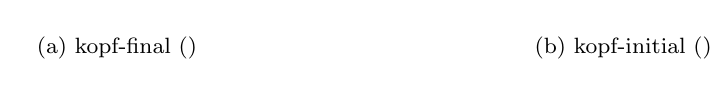
\begin{tikzpicture}
\node [below = 5.8em] (a) {\footnotesize{(a) kopf-final (\hai{{\OV}})}};
\Tree [.VP [.$\triangle$ ] 
             [.\textsc{V'} [.\textsc{XP} ] [.V° ]]
        ]
\begin{scope}[xshift=6cm]
 \node [below = 5.8em] (b) {\footnotesize{(b) kopf-initial (\hai{{\VO}})}};
\Tree  [.VP [.$\triangle$ ] 
             [.\textsc{V'} [.V° ] [.\textsc{XP} ]]
        ]
\end{scope}


\end{tikzpicture}\caption{Die \hai{VP} in \hai{{\OV}}- und \hai{{\VO}}-Sprachen 
%(vgl.\, \citealt[262, Abbildung 1]{Santorini1993a})
}\label{kopfxbar}
 \end{center}
 \end{figure}

 
 


 
 
  In \hai{{\VO}}-Sprachen gibt es keine Varianz in der Verbabfolge. Das moderne Jiddische, welches in dieser Arbeit den Argumenten Santorinis (\citeyear{Santorini1993b}) und Haiders (\citeyear{Haider2013}) folgend als gemischte \hai{{\OV}}/\hai{{\VO}}-Sprache typisiert wird, zeigt somit auch im Verbalkomplex Strukturen beider Grundwortstellungstypen (\ref{dreiverben_oj}). Allein damit, dass im Ostjiddischen Verbstellungsvariation vorliegt, ist eine \hai{{\VO}}-Grundwort-stellung für diese Sprache auszuschließen. Im Bereich der Verbserialisierung verhält sich \ili{Ostjiddisch} eher einer \hai{{\OV}}-Sprache entsprechend (vgl.\, \citealt[170–173]{Geilfuss1990}). 
 
  \eenumsentence{\label{dreiverben_dt} 
      \item dt. \textit{Ein Haus muss} \textit{gebaut}\textsubscript{2} werden\textsubscript{1}\\
     (zitiert n. Vikner 2001:\,75)\label{AbfolgeVerben_1}
    \item dt. *\textit{Ein Haus muss} \textit{werden}\textsubscript{1} \textit{gebaut}\textsubscript{2}\\
     (zitiert n. Vikner 2001:\,75)\label{AbfolgeVerben_2}
  }
  
  
      \eenumsentence{\label{dreiverben_ndl} 
   \item {\ndl} \textit{Een huis moet} \textit{gebouwd}\textsubscript{2} \textit{worden}\textsubscript{1}\\
     (zitiert n. Vikner 2001:\,75)\label{AbfolgeVerben_5}
  \item {\ndl} \textit{Een huis moet} \textit{worden}\textsubscript{1} \textit{gebouwd}\textsubscript{2}\\
     (zitiert n. Vikner 2001:\,75)\label{AbfolgeVerben_6}
}

       
   \eenumsentence{\label{dreiverben_oj} 
     \item {\oj} \textit{A hoyz muz} \textit{geboyt}\textsubscript{2} \textit{vern}\textsubscript{1}\\
     (zitiert n. Besten \& Moed-van Walraven 1986:\,117. Bsp. 16;\\ vgl.\, Vikner 2001:\,74)\label{AbfolgeVerben_7}
     
     \item {\oj} \textit{A hoyz muz} \textit{vern}\textsubscript{1} \textit{geboyt}\textsubscript{2}\\ 
     (zitiert n. Besten \& Moed-van Walraven 1986:\,117. Bsp. 16;\\ vgl.\, Vikner 2001:\,74)\label{AbfolgeVerben_8}

   }
  
     \eenumsentence{\label{dreiverben_engl} 
   \item {\engl} *\textit{A house must} \textit{built}\textsubscript{1} \textit{be}\textsubscript{2}\\
   (zitiert n. Besten \& Moed-van Walraven 1986:\,117. Bsp. 16;\\ vgl.\, Vikner 2001:\,74)\label{AbfolgeVerben_3}
   \item {\engl} \textit{A house must} \textit{be}\textsubscript{1} \textit{built}\textsubscript{2}\\
   (zitiert n. Besten \& Moed-van Walraven 1986:\,117. Bsp. 16;\\ vgl.\, Vikner 2001:\,74)\label{AbfolgeVerben_4}
} 
 
  \eenumsentence{\label{dreiverben_fr} 
     \item {\fr} *\textit{Une maison doit} \textit{construite}\textsubscript{2} \textit{être}\textsubscript{1}\label{AbfolgeVerben_11}
     
     \item {\fr} \textit{Une maison doit} \textit{être}\textsubscript{1} \textit{construite}\textsubscript{2}\\ 
   
     }

 
 Die ostjiddischen Abfolgemuster unterscheiden sich jedoch stark vom Westjiddischen. Zwar stehen noch detaillierte Analysen zur Verbsyntax des späten Westjiddischen aus, doch konnte Santorini (1989, 1992, 1993a, 1993b, 1994, insbes. 1995) zeigen, dass sich die kopf-initiale Verbstellung im Ostjiddischen bereits Ende des 16. Jahrhunderts gegenüber der kopf-finalen Verbstellung durchsetzen konnte, während im Westjiddischen zwischen dem  16. und 17. Jahrhundert noch beide Strukturen bis ins 18. Jahrhundert – für das 19. und 20. Jahrhundert hat Santorini keine Daten zum Westjiddischen – konkurrierten. Ihre Quellen zum Westjiddischen zeigen prinzipiell eine stärkere Ausrichtung am deutschen System als die ostjiddischen Quellen. Für das späte \ili{Westjiddisch} des 19. Jahrhunderts ist eher eine kopf-finale Grundstruktur anzunehmen als eine kopf-initiale.


 \hai{{\OV}}-Sprachen erlauben im Gegensatz zu \hai{{\VO}}-Sprachen mehr Wortstellungsvariation. Die Abweichung der Grundstellung der Verben innerhalb der \hai{{\RSK}} wird als \quein{verb raising} (\hai{{\VR}}) bezeichnet (vgl.\, \citealt{Evers1975};Abbildung \ref{baumVR}). In einer \hai{{\OV}}-Sprache wie dem Deutschen ist die übliche Abfolge bei zweigliedrigen Verbketten \hai{V}\textsubscript{2}–\hai{V}\textsubscript{1} (s. Abschnitt \,%rs Abschnitt
 \ref{Verbabfolgedeutsch}, S.\, \pageref{Verbabfolgedeutsch}). Unter \hai{{\VR}} fallen damit Belege des Musters \hai{V}\textsubscript{1}–\hai{V}\textsubscript{2}, wie in (\ref{BSPVR12}) illustriert. 


  \eenumsentence{\label{BSPVR}
    \item dt. \textit{Da habt ihr mir nicht folgen}\textsubscript{2} \textit{wollen}\textsubscript{1}\label{BSPVR21}  
       \item dt. \textit{Da habt ihr mir nicht wollen}\textsubscript{1} \textit{folgen}\textsubscript{2}\label{BSPVR12}
  }
  

\vspace{0.2cm}
 


\begin{figure}

\fittable{
\begin{tikzpicture}[sibling distance=36pt] 
 \Tree [.VP\textsubscript{1} [.VP\textsubscript{2} [.VP\textsubscript{3} [.\node(V3){\=V\textsubscript{3}};V\textsubscript{3} ] ] 
 [.\=V\textsubscript{2} \node(V1){V\textsubscript{2}};] ] 
[.\node(v1g){\=V\textsubscript{1}};V\textsubscript{1} ]
]
\draw[semithick,->] (V3) to[bend right=20] (V1);
%[.V\textsubscript{1} V\textsubscript{1} ]]

\begin{scope}[xshift=4cm,yshift=12pt]
 \tikzset{every tree node/.style={align=center, anchor=north}}
\Tree [.VR\\[14pt]{$\Rightarrow$} ]
\end{scope}

\begin{scope}[xshift=10cm]
 \Tree [.VP\textsubscript{1} [.\node(vp2g){VP\textsubscript{2}};[.VP\textsubscript{3} e ] [.\node(V2){\=V\textsubscript{2}}; [.V\textsubscript{2} [.V\textsubscript{2} ] [.\=V\textsubscript{3} V\textsubscript{3} ]
] ] ] 
[.\=V\textsubscript{1} \node(V1){V\textsubscript{1}};]
]
\draw[semithick,->] (V2) to[bend right=20] (V1);

\end{scope}

 \end{tikzpicture}
\caption{\hai{{\VR}} nach den Besten \& Edmondson 
 (\citeyear[196, Abbildung 76]{BestenEdmondson1983})}
\label{baumVR}	%Baum
}

 \end{figure}


 In älteren Sprachstufen des Jiddischen findet sich bereits \hai{{\VR}} belegt, wie in (\ref{IPPsantorinib}) ( \ref{IPPsantorini}) (S.\, \pageref{IPPsantorini})  zu sehen ist (vgl.\, \citealt{Santorini1989,Santorini1992,Santorini1993b,Santorini1993a,Santorini1994,Santorini1995}). \hai{{\VR}} ist auch vielfach für die Diachronie des Deutschen beschrieben und analysiert worden (vgl.\, \citealt{Maurer1926,Haerd1981,Ebert1980,Ebert1981,Ebert1998,Agel2001,Ramers2005,Axel2007,Sapp2006,Sapp2011}). Während das Schriftdeutsche im Verlauf des Frühneuhochdeutschen die relativ strikte Abfolge \hai{V}\textsubscript{2}–\hai{V}\textsubscript{1} durchsetzt,\footnote{Krasselt (\citeyear{Krasselt2013}) zeigt, dass selbst noch in der modernen Umgangssprache des Deutschen Variation und eine breite Akzeptabilität bei Zwei- und Dreiverbclustern besteht.} entwickelt sich das Jiddische komplementär und baut die \hai{V}\textsubscript{1}–\hai{V}\textsubscript{2} Serialisierung weiter aus. Im modernen Ostjiddischen ist damit die Grundstellung des Deutschen nicht gegeben;\, hier sind beide Abfolgevarianten möglich (\ref{BSPVRJI}) (vgl.\, \citealt{Santorini1989,Santorini1992,Santorini1993b,Santorini1993a,Santorini1994,Santorini1995,BestenWalraven1986}). 
  
  
   \eenumsentence{\label{BSPVRJI}
   
    \item {\mj} \textit{da habt ir mir nit veln}\textsubscript{1} \textit{falgn}\textsubscript{2} (\hai{DCY}:\,{\wj}\,Gerichtsprotokolle von 1465)\\
   \sem{da habt ihr mir nicht folgen wollen (wörtl. wollen folgen)}\label{IPPsantorinib}

    \item {\oj} {\RL{ד{א\makebox(-1.25,-1.25)[r]{\libertineGlyph{uni05B8}}} ה{א\makebox(-1.25,-1.25)[r]{\libertineGlyph{uni05B8}}}בט איר מיר ניט געוו{א\makebox(-1.25,-1.25)[r]{\libertineGlyph{uni05B8}}}לט {פ\makebox(-0.8,9)[r]{\libertineGlyph{uni207B}}}{א\makebox(-1.25,-1.25)[r]{\libertineGlyph{uni05B8}}}לגן}} \textit{do hobt ir mir nit gevolt}\textsubscript{2} \textit{folgn}\textsubscript{1}\\
     \sem{da habt ihr mir nicht folgen wollen (wörtl. gewollt folgen)} \label{BSPVRji21}  
       \item {\oj} {\RL{ד{א\makebox(-1.25,-1.25)[r]{\libertineGlyph{uni05B8}}} ה{א\makebox(-1.25,-1.25)[r]{\libertineGlyph{uni05B8}}}בט איר מיר ניט {פ\makebox(-0.8,9)[r]{\libertineGlyph{uni207B}}}{א\makebox(-1.25,-1.25)[r]{\libertineGlyph{uni05B8}}}לגן געוו{א\makebox(-1.25,-1.25)[r]{\libertineGlyph{uni05B8}}}לט}} \textit{do hobt ir mir nit folgn}\textsubscript{1} \textit{gevolt}\textsubscript{2}\\ 
       \sem{da habt ihr mir nicht folgen wollen (wörtl. folgen gewollt)}\label{BSPVRji12}   
       
                }
  
  
Die deutschen Dialekte (und auch andere westgermanische Varietäten) zeigen eine deutlich höhere Variabilität innerhalb der \hai{VP}, als es die moderne Schriftsprache vermuten lässt (u.\,a.\, \citealt{Loetscher1978,BestenEdmondson1983,Patocka1997,Vikner1995,Vikner2001,Seiler2004,Wurmbrand2004,Wurmbrand2006,Wurmbrand2012,Sapp2006,Sapp2011,DubenionSmith2010,Schallert2014}). Die Möglichkeit, dass \hai{{\VR}}-Belege des \hai{chrLiJi1} auf deutsch-dialektalen Formen fußen, ist damit nicht auszuschließen. Doch auch in Quellen des späten Westjiddischen finden sich beide Abfolgetypen (\hai{V}\textsubscript{2}–\hai{V}\textsubscript{1} u. \hai{V}\textsubscript{1}–\hai{V}\textsubscript{2}) belegt ( \ref{GrobVRnegation}), (weitere Bsp. vgl.\, \citealt[36–38]{Schaefer2008}, \citeyear[61f]{Schaefer2010}). Das heißt, dass wir \hai{{\VR}} im \hai{{\LiJi}} sowohl als Reflexe aus ostjiddischen, westjiddischen als auch deutschen Varietäten interpretieren können. 
  
   \eenumsentence{
  

 \item {\RL{דא\makebox(-1.25,-1.15)[r]{\libertineGlyph{uni05B7}}ס קא\makebox(-1.25,-1.15)[r]{\libertineGlyph{uni05B7}}הנער קא\makebox(-1.25,-1.15)[r]{\libertineGlyph{uni05B7}}הן מא\makebox(-1.25,-1.15)[r]{\libertineGlyph{uni05B7}}ן מיט ניקס ז{א\makebox(-1.25,-1.25)[r]{\libertineGlyph{uni05B8}}}לל נעממע}} \\
       \textit{das kahner kahn man mit niks soll nemme}\\
       \sem{dass keiner einen Mann ohne etwas nehmen soll}\\
       (\qu{Die Hochzeit zu Grobsdorf} Gießen 1822:\,12)\label{GrobVRnegation}
  }

  
 Semantische Verbklassen spielen beim \hai{{\VR}} deutscher Varietäten eine große Rolle (\citealt{Ebert1998,Sapp2006,Sapp2011,Vikner2001,Wurmbrand2004,Wurmbrand2006,Schallert2014}). Allerdings kann diese Arbeit aus folgenden Gründen selbst keine Analyse der Beziehung von \hai{{\VR}} und semantischer Verbklassen im \hai{{\LiJi}} leisten: Zum einen fehlen detaillierte und v.\,a.\, flächendeckende Daten zur Situation von \hai{{\VR}} in den deutschen Dialekten, mit denen die Belege aus dem \hai{chrLiJi1} zu vergleichen wären. Zum anderen sind die Korpora des \hai{{\LiJi}} allein vom Umfang her zu heterogen, um repräsentativ für ein System sein zu können. Besonders frequente Verben, wie etwa Modalverben (vgl.\, \citealt{Ruoff1981}), wären so von vornherein deutlich überrepräsentiert, während andere Verbklassen unter Umständen vom \isi{Korpus} gar nicht erfasst wären. Auch hätten im Fall einer \hai{{\VR}}-Analyse nach semantischen Rollen alle Belege für die schriftdeutsche Grundabfolge \hai{V}\textsubscript{2}–\hai{V}\textsubscript{1} aufgenommen und annotiert werden müssen. Und auch Belege für \hai{{\VR}} außerhalb des \hai{{\LiJi}}, also in der Literatursprache des 19. Jahrhunderts, hätten miterhoben werden müssen. Die nachfolgende Analyse beschreibt somit allgemein die Existenz von \hai{{\VR}} im \hai{{\LiJi}}, nicht aber deren hintergründige Motivation (Verbklasse, \hai{{\VR}} in der Schriftsprache). 


 
 \subsection{Abfolge zweigliedriger Verbcluster}\label{vr}
 %  %\noindent   
   Die Verbserialisierung \hai{V}\textsubscript{1}–\hai{V}\textsubscript{2}, die ausgehend von der Organisation der neuhochdeutschen \hai{VP} durch \hai{{\VR}} entsteht, findet sich in 29 Quellen (54,7\,\%) des \hai{chrLiJi1}-\isi{Korpus}. Die zeitliche Verteilung der Belege erstreckt sich über den gesamten Untersuchungszeitraum (Abbildung \ref{histoVR}), allerdings zeigt sich eine besondere Anhäufung an Quellen, die diese Manipulationsstrategie aufweisen, in der ersten Hälfte des 19. Jahrhunderts.\, Auch die areale Verteilung der Texte mit \hai{{\VR}}-Strukturen erstreckt sich auf das gesamte Erhebungsgebiet (Abbildung \ref{KarteVR}). 
    
    \begin{figure}
   \fittable{    
	\begin{tikzpicture}
		\begin{axis}[only marks, width=0.82\textwidth,height=0.2\textheight,
		legend style={at={(1,1)},xshift=+0.2cm, yshift=-0.02cm,anchor=north west,nodes=left},
			%title={Funktionstypen des sp\"aten Westjiddisch},
			xtick={1700, 1725, 1750, 1775, 1800, 1825, 1850, 1875, 1900, 1925, 1950, 1975}, ytick=\empty,
			x tick label style={/pgf/number format/1000 sep=}, 
			y tick label style={/pgf/number format/1000 sep=},
			%extra y ticks={456.1, 1022.4},
			%extra y tick labels={{456,1},{1022,4}},
			extra y tick style={grid=major,
				tick label style={, ,}},
				ymin=0.5,
				ymax=2.5,
			ylabel={Phänomenbelege},
			enlarge x limits=0.03]	
		



\addplot  [mark=square, black] table [x=jahr, y=vr] {figures/VR_vr.txt};%2


\addplot [mark=o,black] table [x=jahr, y=no] {figures/VR_no.txt};%1
 

			% Andere Formen a={mark=square*,blue},% b={mark=triangle*,red},% c={mark=o,draw=black}}
						\legend{Abfolge \hai{V}\textsubscript{1}–\hai{V}\textsubscript{2} (\hai{{\VR}}), keine \hai{VR}} %macht Legende
		\end{axis}
	\end{tikzpicture}	
	}
	\caption{Diachrone Verteilung von \hai{{\VR}} bei zweigliedrigen Verbketten im \hai{chrLiJi1}}
	\label{histoVR}	
\end{figure}

    

 
\begin{figure}
\centering
\includegraphics[width=\textwidth]{figures/Karte_VR2.png}
		\caption{\label{KarteVR} Areale Verteilung von \hai{{\VR}} bei zweigliedrigen Verbketten im \hai{chrLiJi1}}
	\end{figure}
  %farbe angleichen



    
    
    Im \hai{jüdLiJi1} ist in neun von zehn Quellen \hai{{\VR}} anzutreffen. Einzig die ungarische Quelle \hai{PDebrecen} unterlässt Manipulationen der Verbserialisierung.\footnote{Diese Quelle zeigt auch bezüglich mehrgliedriger (> 2) \isi{Verbcluster} keine Manipulationen, vgl.\, Unterabschnitt \ref{verbcluster}. \,%rs Unterabschnitt
    Dies ist besonders vor dem Hintergrund interessant, dass Ungarisch, die hier koterritoriale Sprache, auch Varianz im Verbkomplex aufweist (\citealt{Bartos2004}).} 

\subsection{Abfolge mehrgliedriger Verbcluster}\label{verbcluster}%
 %  %\noindent 
 Das moderne Jiddische zeigt, wie schon die Zweiverbcluster vermuten lassen (vgl.\, Unterabschnitt \ref{vr}), \,%rs Unterabschnitt
 starke Varianz bezüglich mehrgliedriger Verbgefüge. Noch fehlt es an Untersuchungen, die Präferenz und Akzeptanz der möglichen Abfolgevarianten erfassen. In der grammatiktheoretischen Literatur finden sich zwei Typen von Dreiverbclustern belegt, und zwar \hai{V\textsubscript{1}}–\hai{V\textsubscript{2}}–\hai{V\textsubscript{3}} und \hai{V\textsubscript{1}}–\hai{V\textsubscript{3}}–\hai{V\textsubscript{2}}  (\citealt[117]{BestenWalraven1986}; \citealt[70–79]{Vikner2001}). Die Situation im Alt- und Mitteljiddischen im \hai{DCY} wurde von Santorini (\citeyear{Santorini1995, Santorini1994, Santorini1993b, Santorini1993a, Santorini1992, Santorini1989}) zwar nicht nach der Statustheorie Bechs (\citeyear{Bech1955,Bech1957}) beschrieben. Ihre Daten zeigen aber immerhin einen Wandel von kopf-finalen (\hai{{\OV}}) zu kopf-initialen (\hai{{\VO}}) Strukturen bei \textit{komplexen Verben} (\qu{complex verbs}), der bereits im Mitteljiddischen einsetzt und Ende des 18. Jahrhunderts vollständig abgeschlossen war (s. u.\,a.\, \citealt[270]{Santorini1993a}). 
Es ist durchaus plausibel, dass Abfolgevarianz innerhalb der \hai{VP}, wie wir sie im gegenwärtigen Ostjiddischen finden, auch im späten Westjiddischen gegeben war. Analysen zu \hai{{\VR}} im späten Westjiddischen bestätigen dies (\citealt[36–38]{Schaefer2008}; \citealt[61f]{Schaefer2010}). Allerdings ist auch hier das letzte Wort längst nicht gesprochen. 

Manipulationen bei mehrgliedrigen Verbclustern (> 2) finden sich in lediglich neun Quellen des \hai{chrLiJi1};im \hai{jüdLiJi1} betrifft es immerhin fünf der zehn Quellen. 
Im \hai{chrLiJi1} tritt interessanterweise nur eine von der Matrixsprache abweichende Serialisierungsvariante auf. Es handelt sich dabei um für \hai{{\VO}}-Sprachen typische Abfolge \hai{V\textsubscript{1}}–\hai{V\textsubscript{2}}–\hai{V\textsubscript{3}}–\hai{V\textsubscript{n}}. In sieben Quellen findet sich diese Form von \hai{{\VR}} bei Dreiverbclustern mit \isi{Ersatzinfinitiv} (\hai{{\IPP}})\footnote{Zur näheren Erklärung siehe Abschnitt \ref{noipp}, S.\, \pageref{noipp}.} wie etwa in (\ref{bsp321_1}).\footnote{D.\,h. die Matrixabfolge wäre hier \hai{V\textsubscript{1}}–\hai{V\textsubscript{3}}–\hai{V\textsubscript{2}} (vgl.\, Abschnitt \ref{noipp}, S.\, \pageref{noipp}).} 
 In drei Quellen tritt die \hai{{\VO}}-Abfolge im Futur auf, wie in (\ref{bsp321_2}). In einer Quelle (\hai{AO} Wien, 1770) tritt diese Abfolge in  Futur- und in \hai{{\IPP}}-Kontext auf. In einem Beispiel finden wir die \hai{{\VO}}-Abfolge bei einem viergliedrigen \isi{Verbcluster} (\ref{bspvierverbcluster}).\footnote{Dieser Beleg ist der einzige für eine Manipulation eines viergliedrigen Verbclusters.} In der Quelle \hai{{\PP}} findet sich in einem einzigen Beleg die \hai{{\VO}}-Struktur mit einem trunkierten Ersatzinfitiv von \sem{sollen} (\ref{bsp312_1}), wie es aus dem Südniederländischen und dem mittel- und südbairischen Übergangsgebiet bekannt ist (vgl.\, \citealt{Hoehle2006}\,;\, \citealt{Weber2014,Schallert2013}, \citeyear[188]{Schallert2014}). Acht der neun Quellen, in denen sich \hai{V\textsubscript{1}}–\hai{V\textsubscript{2}}–\hai{V\textsubscript{3}}(–\hai{V\textsubscript{4}}) findet, weisen auch \hai{{\VR}} bei zweigliedrigen Verben auf (vgl.\, Unterabschnitt \ref{vr}). Damit wird deutlich, dass sich die Manipulation von zweigliedrigen Verbketten nicht von denen mehrgliedriger Cluster unterscheidet. Auffällig sind die Tendenzen im \hai{{\LiJieins}}, die \hai{VP} nach dem \hai{{\VO}}-Muster zu strukturieren. In vielen Fällen kommen Extrapositionen hinzu, die zusammen mit der Abfolge innerhalb der \hai{VP} die \textit{Illusion} eines Satzes mit \hai{{\VO}}-Grundwortstellung evozieren, wie z.\,B.\, in (\ref{bsp321_1}) und (\ref{bsp312_1}). 

    
     %lea2
      \eenumsentence{
       \item \textit{daß mer nich hat\textsubscript{1} sollen\textsubscript{2} seh'n\textsubscript{3} den ßerrissenen Brustmalbisch} (\hai{SV} München, 1890:\,10)\\
     wörtl. \sem{dass man nicht hat sollen sehen die zerrissene Weste}\label{bsp321_1} 
     
\item \textit{weil er sich will\textsubscript{1} lassen\textsubscript{2} beschneiden\textsubscript{3}} (\hai{TH} Merseburg, 1820:\,98)\label{bsp321_2}

    \item  \textit{ich hab'\textsubscript{1} wölle\textsubscript{2} anheibe\textsubscript{3} zu hupfe\textsubscript{4}} (\hai{PG} Speyer, 1835:\,54)\\
  wörtl. \sem{ich habe wollen anfangen zu hüpfen}\label{bspvierverbcluster}
  
  \item  \textit{der hat\textsubscript{1} soll\textsubscript{2} gehören\textsubscript{3} der Schönsten} (\hai{{\PP}} Berlin, 1839:\,17)\\
 \sem{der hat der Schönsten gehören sollen}\label{bsp312_1}
      }


      
Das Raumbild dieser Manipulationsstrategie lässt ein grobflächiges Areal erkennen (Abbildung \ref{KarteVerbcluster}): Die Abfolge \hai{V\textsubscript{1}}–\hai{V\textsubscript{2}}–\hai{V\textsubscript{3}} im Futur ist ausschließlich in Quellen des Südostens belegt. M.\,E. aber ist auch dieses Gebiet mehr ein Zufallsprodukt. Viel aussagekräftiger ist die Interpretation der Karte in Abbildung \ref{KarteVerbcluster} bezüglich der Grundstruktur: Die Abfolge \hai{V\textsubscript{1}}–\hai{V\textsubscript{2}}–\hai{V\textsubscript{3}} tritt im \hai{chrLiJi1} unabhängig der Quellverortung auf. 


\begin{figure}
\centering
\includegraphics[width=\textwidth]{figures/Karte_VR_verbcluster.png}
		\caption{\label{KarteVerbcluster} Areale Verteilung von Abfolgevarianzen zwei- u. mehrgliedriger \isi{Verbcluster} im \hai{chrLiJi1}}
	\end{figure}
  %farbe angleichen
 
 
Mit Blick auf die Verteilung von \hai{{\VR}} bei mehrgliedrigen Verbketten in der Zeit (Abbildung \ref{histoVerbcluster}) fällt auf, dass die \hai{{\VO}}-Abfolge (\hai{V\textsubscript{1}}–\hai{V\textsubscript{2}}–\hai{V\textsubscript{3}}–\hai{V\textsubscript{n}}), analog zur Zweiverbserialisierung (\hai{V\textsubscript{1}}–\hai{V\textsubscript{2}}) im gesamten Untersuchungszeitraum auftritt. 
     
    \begin{figure}
\fittable{
	\begin{tikzpicture}
		\begin{axis}[only marks, width=0.82\textwidth,height=0.24\textheight,
		legend style={at={(1,1)},xshift=+0.2cm, yshift=0cm,anchor=north west,nodes=left},
			%title={Funktionstypen des sp\"aten Westjiddisch},
			xtick={1700, 1725, 1750, 1775, 1800, 1825, 1850, 1875, 1900, 1925, 1950, 1975}, ytick=\empty,
			x tick label style={/pgf/number format/1000 sep=}, 
			y tick label style={/pgf/number format/1000 sep=},
			%extra y ticks={456.1, 1022.4},
			%extra y tick labels={{456,1},{1022,4}},
			extra y tick style={grid=major,
				tick label style={, ,}},
				ymin=0.5,
				ymax=4,
                y=8.4mm,
			ylabel={Phänomenbelege},
			enlarge x limits=0.03]	
	
		



\addplot  [mark=square, black] table [x=jahr, y=vr] {figures/VR_vr_123.txt};%3.5
\addplot  [mark=*, red] table [x=jahr, y=123IPP] {figures/cluster_123IPP.txt};%3
\addplot  [mark=*, orange] table [x=jahr, y=123keinIPP] {figures/cluster_123keinIPP.txt};%.2.5
\addplot  [thick, mark=*, green] table [x=jahr, y=312status] {figures/cluster_312status.txt};%2
\addplot  [thick, mark=*, yellow] table [x=jahr, y=1234] {figures/cluster_1234.txt};%1.5

\addplot  [mark=o, black] table [x=jahr, y=no] {figures/cluster_no.txt};%1


 

			% Andere Formen a={mark=square*,blue},% b={mark=triangle*,red},% c={mark=o,draw=black}}
				\legend{\hai{V}\textsubscript{1}–\hai{V}\textsubscript{2} (vgl.\, Abbildung \ref{KarteVR}), \hai{V}\textsubscript{1}–\hai{V}\textsubscript{2}–\hai{V}\textsubscript{3} (\hai{{\IPP}}), \hai{V}\textsubscript{1}–\hai{V}\textsubscript{2}–\hai{V}\textsubscript{3} (Futur), \hai{V}\textsubscript{1}–\hai{V}\textsubscript{2}–\hai{V}\textsubscript{3} (trunkierter \hai{{\IPP}}), \hai{V}\textsubscript{1}–\hai{V}\textsubscript{2}–\hai{V}\textsubscript{3}–\hai{V}\textsubscript{4}, keine Manipulation} %macht Legende
		\end{axis}
	\end{tikzpicture}
}
	\caption{Diachrone Verteilung von Abfolgevarianz mehrgliedriger \isi{Verbcluster} im \hai{chrLiJi1}}
	\label{histoVerbcluster}	
\end{figure}

 
Wie auch im \isi{Korpus} christlicher Autoren, so finden wir im \hai{jüdLiJi1} ausschließlich Manipulationen der Verbserialisierung nach dem \hai{{\VO}}-Typ (\hai{V}\textsubscript{1}–\hai{V}\textsubscript{2}–\hai{V}\textsubscript{3}): fünf der zehn Quellen weisen diese Abfolge auf.\footnote{Es handelt sich dabei um die Quellen: \hai{GuS10}, \hai{PBreslau}, \hai{PBerlin1} (im \hai{{\IPP}}-Kontext), \hai{PBerlin2} (im Futur-Kontext) u. \hai{PAlsleben} (im \hai{{\IPP}}-Kontext mit \isi{Partizip}, vgl.\, \ref{noipp}).}
 
 %Die Abwesenheit von \hai{{\VR}} bei mehrgliedrigen Verbklustern im \hai{LiJi2} ist schwer einzuschätzen. %BB erklären/diskutieren wieso nicht im \ili{LiJi2} manipuliert!?
 
 Das Auftreten von \hai{{\VR}} im \hai{{\LiJi}} ist ein besonders gutes Beispiel für die 
Nutzung der Viskosität sprachlicher Strukturen (vgl.\, \citealt{Haider2007}). Die Organisation der \hai{{\RSK}} im Deutschen ist alles andere als auf die Verbabfolge \hai{V}\textsubscript{2}–\hai{V}\textsubscript{1}  der Schreibnorm festgelegt, sondern erlaubt viel mehr Variation, was mit Blick auf sprachgeschichtliche und dialektale Daten deutlich wird. Das \hai{{\LiJi}} nutzt diese Variabilität (Viskosität) aus, um entweder Formen (ost-)jiddischer \isi{Syntax} zu emulieren und/oder um durch den Kontrast zur Schreibsprache Fremdheit und/oder Fehlerhaftigkeit zu erzeugen. 

 
 
 
 
  \subsection{Rechtsadjazenz trennbarer Verbpartikeln}\label{rechtsadjazent}
  %  %\noindent
Wie alle germanischen Sprachen 
% hat auch Jiddisch 
verfügt auch das Jiddische über %\todo{rephrase}
trennbare und nicht-trennbare Verb\-partikeln (\citealt[33–49]{Vikner2001}). Jiddisch verhält sich in vielerlei Hinsicht ähnlich dem Schriftdeutschen (\citealt[33–49]{Vikner2001}). Besonders die verschiedenen möglichen Stellungsvarianten von trennbarer \isi{Partikel} und Verb im Satz scheinen keine Unterschiede zwischen Deutsch und Jiddisch aufzuweisen (vgl.\, \citealt[38f]{Heine2010}; \citealt[33–49]{Vikner2001}). Vor diesem Hintergrund mag es überraschen, dass in einer Vielzahl literaturjiddischer Quellen eine Manipulation an der schriftsprachlichen Position von trennbaren Verbpartikeln erfolgt. Auffällig ist dabei die Einheitlichkeit aller betroffenen Texte. Obwohl die \isi{Verbpartikel} im deutschen Satz durchaus an mehreren Positionen stehen kann (vgl.\, \citealt{Heine2010,Luedeling2001}), d.\,h. der theoretisch mögliche Raum für Manipulationen recht groß ist, findet sich im \hai{{\LiJi}} nur eine vom Standard abweichende Position der \isi{Partikel}, nämlich die rechts des Verbs in nicht-\hai{V2}-Kontexten, in denen das Partikelverb in der \hai{{\RSK}} steht, s. (\ref{particl_liji}). \,%rs + s.
 Im \hai{chrLiJi1} finden sich solche rechtsadjazenten Verbpartikeln bei 24 verschiedenen Verben in nicht-\hai{V2}-Kontexten bei insgesamt neun Quellen z.\,B.\, (\ref{particl_liji_1})–(\ref{particl_liji_2}), im \hai{jüdLiJi1} in drei Quellen,\footnote{Diese Quellen sind: \hai{\hai{PAlsleben}, \hai{PBerlin1}, \hai{PBerlin2}.}} z.\,B.\, \ref{particl_liji_3}. 

Aus den deutschen Dialekten können solche Formen nicht entlehnt sein.\footnote{Ein Beispiel dafür, dass die dt. Dialekte in diesem Fall wie die Schriftsprache funktionieren, findet sich im \hai{WS} 16 \qu{Du bist noch nicht groß genug, um eine Flasche Wein auszutrinken}. Hier taucht die Abfolge, in der die \isi{Partikel} rechtsadjazent steht, \quein{zu trinken aus} lediglich in den dänischsprachigen und zimbrischen Bögen auf, in den deutschsprachigen Bögen bleibt die \isi{Partikel} links am Verb (s. Abschnitt \ref{v2}, S.\, \pageref{WS16}).}\\\,%rs Spatium fehlt


   
\eenumsentence{\label{particl_liji}

\item \textit{wär ich gegange doch nich mit} (\hai{LS} Bonn, 1925:\,17)\\
 \sem{wär ich doch nicht mitgegangen}\label{particl_liji_1}

\item \textit{ich muß das Fett nur schöpfen ab} (\hai{HJ} Berlin, 1811:\,101)\\
 \sem{ich muss das Fett nur abschöpfen}\label{particl_liji_2}

\item \textit{woribber ich jedoch stimm an kaane Klagelider} (\hai{PAlsleben}:\,5)\\
 \sem{worüber ich jedoch keine Klagelieder anstimme}\label{particl_liji_3}

\item \textit{Woß du willst von der noch holen raus?} (\hai{TFRdt}:\,35)\\
 \sem{Was willst du von der noch heraus holen?}\label{particl_liji_4}
 
}


An der diachronen Verteilung der Belege auffällig ist, dass rechtsadjazente Verbpartikeln besonders häufig um 1800 auftreten und nur noch vereinzelt in der 2. Hälfte des 19. Jahrhunderts. Für das 20. Jahrhundert ist nur mehr ein einzelner Beleg vorhanden (vgl.\, Abbildung \ref{histoparticl}). 
Auch die Kartierung der Belege zeigt ein durchaus interessantes Raumbild (Abbildung \ref{KarteVerbpartikel}). Rechtsadjazente Verbpartikeln trennbarer Verben finden sich besonders im östlichen Teil des Untersuchungsgebiets und besonders im nordöstlichen Raum. Was diesem Raumbild jedoch zugrunde liegt, ist fragwürdig. Ohne in die Irre laufende Spekulationen zuzulassen, lässt sich zumindest am Raumbild feststellen, dass besonders die Randgebiete des Untersuchungsgebietes betroffen sind und damit Kontaktzonen zu Sprachen mit einer anderen Grundwortstellung als dem Deutschen betroffen sind. Das hieße, dass hier ggf. Strukturen aus dem Kontakt zu anderen Sprachen als dem Jiddischen ins \hai{{\LiJieins}} einfließen. Die zeitliche Verteilung bestärkt dies insofern, als die Belege im Zeitraum der napoleonischen Kriege und damit zu einer Zeit, in der der Kontakt zu anderen Sprachen begünstigt war, auftreten. Wie Skibicki (\citeyear[142]{Skibicki2013}) zeigt, ist die rechtsadjazente Positionierung von Verbpartikeln aus der \hai{DaF}-Forschung besonders als Interferenz von Muttersprachlern des Polnischen \il{polnisch} bekannt. Im Polnischen sind Partikelverben nicht trennbar. Dies könnte zumindest die Belege im Osten des Untersuchungsgebietes erklären. 
  \begin{figure}
\fittable{
	\begin{tikzpicture}
		\begin{axis}[only marks, width=0.82\textwidth,height=0.2\textheight,
		legend style={at={(1,1)},xshift=+0.2cm, yshift=-0.0cm,anchor=north west,nodes=left},
			%title={Funktionstypen des sp\"aten Westjiddisch},
			xtick={1700, 1725, 1750, 1775, 1800, 1825, 1850, 1875, 1900, 1925, 1950, 1975}, ytick=\empty,
			x tick label style={/pgf/number format/1000 sep=}, 
			y tick label style={/pgf/number format/1000 sep=},
			%extra y ticks={456.1, 1022.4},
			%extra y tick labels={{456,1},{1022,4}},
			extra y tick style={grid=major,
				tick label style={, ,}},
				ymin=0.5,
				ymax=2.5,
			ylabel={Phänomenbelege},
			enlarge x limits=0.03]	
	
		

\addplot  [mark=*, black] table [x=jahr, y=particl] {figures/particl_particl.txt};%2
\addplot [mark=o,black] table [x=jahr, y=no] {figures/particl_no.txt};%1
 

			% Andere Formen a={mark=square*,blue},% b={mark=triangle*,red},% c={mark=o,draw=black}}
						\legend{\isi{Partikel} rechtsadjz., keine Manipulation} %macht Legende
		\end{axis}
	\end{tikzpicture}
}
	\caption{Diachrone Verteilung rechtsadjazenter Verbpartikeln trennbarer Verben im \hai{chrLiJi1}}
	\label{histoparticl}	
\end{figure}
     


\begin{figure}
\centering
\includegraphics[width=\textwidth]{figures/Karte_Partikel.png}
		\caption{\label{KarteVerbpartikel} Areale Verteilung rechtdadjazenter Partikeln trennbarer Verben im \hai{chrLiJi1}}
	\end{figure}
  %farbe angleichen

Nach Vikner (\citeyear[36]{Vikner2001}) dürfte man eine solche Position der \isi{Verbpartikel}, wie wir sie im \hai{{\LiJi}} sehen, im modernen Jiddischen nicht annehmen. Wenn in strikten \hai{{\VO}}-Sprachen, wie Dänisch oder Englisch, eine \isi{Verbpartikel} im \hai{V2}-Kontext trennbar ist (\ref{particle_3}), (\ref{particle_4}), dann ist sie es auch im nicht-\hai{V2}-Kontext (\ref{particle_3c}), (\ref{particle_4c}). Im Jiddischen und Deutschen hingegen bleibt eine \isi{Partikel}, die im \hai{V2}-Kontext trennbar ist (\ref{particle_3}), (\ref{particle_4}), im nicht-\hai{V2}-Kontext ungetrennt. %Wobei man an dieser Stelle kritisch fragen muss, wie Vikner (\citeyear[36]{Vikner2001}) hier im modernen Jiddischen, welches symmetrisches \hai{V2} in Haupt- wie Nebensatz hat (vgl.\, \citealt{Santorini1989}), einen nicht-\hai{V2}-Kontext feststellen will. = eingebettete Fragesätze
Es bleibt festzuhalten, dass sich die auffälligen Manipulationen des \hai{{\LiJi}} an Strukturen orientieren, die charakteristisch für  \hai{{\VO}}-Sprachen sind. Gegebenenfalls wollen diese Strukturen also \hai{{\VO}}-Eigenschaften des Jiddischen imitieren. Da sich hier die Partikeln wie in \hai{V2}-Umgebung verhalten, können die literaturjiddischen Belege für rechtsadjazente Verbpartikeln im nicht-\hai{V2}-Kontext auch mit der \isi{Emulation} ostjiddischen symmetrischen \hai{V2} zusammenhängen. 

% \qu{if a German or Yiddish particle is postverbal (seperate) in \hai{V2} contexts, then it is still preverbal (non-separate) in non-\hai{V2} contexts} (\citealt[36]{Vikner2001}). 

   \eenumsentence{ 
   \item dt. \textit{Den Brief schickt er ab} (zitiert n. \citealt[35, Bsp. 62 a.]{Vikner2001})
\label{particle_1}
    \item ji. ??\textit{Dem briv shikt er avek} 
    (zitiert n. \citealt[119, Bsp. 20b.]{BestenWalraven1986};vgl.\, \citealt[35, Bsp. 62 b.]{Vikner2001})\label{particle_2}
 \item {\dän} \textit{Brevet sender han afsted} (zitiert n. \citealt[35, Bsp. 62 c.]{Vikner2001})\label{particle_3}
\item {\engl} \textit{The letter he sends away}\label{particle_4}
  \item dt. *\textit{Den Brief abschickt er} (zitiert n. \citealt[35, Bsp. 62 d.]{Vikner2001})\label{particle_1b}
    \item ji. *\textit{Dem briv avekshikt er} (zitiert n. \citealt[35, Bsp. 62 e.]{Vikner2001})\label{particle_2b}
 \item {\dän} *\textit{Brevet afstedsender han} (zitiert n. \citealt[35, Bsp. 62 f.]{Vikner2001})\label{particle_3b} \,%rs Punkt fehlt
 \item {\engl} *\textit{The letter awaysends he}\label{particle_4b}\\
 } 
   
   
   \eenumsentence{ 
   \item dt. *\textit{Den Brief hat er geschickt ab} (zitiert n. \citealt[36, Bsp. 64 a.]{Vikner2001})\label{particle_1c}
    \item ji. ??\textit{Dem briv hot er geshikt avek} (zitiert n. \citealt[36, Bsp. 64 b.]{Vikner2001})\label{particle_2c}
 \item {\dän} \textit{Brevet har han sendt afsted} (zitiert n. \citealt[36, Bsp. 64 c.]{Vikner2001})\label{particle_3c}
\item {\engl} \textit{The letter he has send away}\label{particle_4c}
  \item dt. \textit{Den Brief hat er abgeschickt} (zitiert n. \citealt[36, Bsp. 64 d.]{Vikner2001})\label{particle_1bb}
    \item ji. \textit{Dem briv hot er avekgeshickt} (zitiert n. \citealt[36, Bsp. 64 e.]{Vikner2001})\label{particle_2bb}
 \item {\dän} *\textit{Brevet har han afstedsendt} (zitiert n. \citealt[36, Bsp. 64 f.]{Vikner2001})\label{particle_3bb} \,%rs Punkt fehlt
 \item {\engl} *\textit{The letter he has awaysent}\label{particle_4bb}\\
   }
   
Bereits die Akzeptabilitätsnotation Vikners (\citeyear{Vikner2001}) für  rechtsadjazente Partikeln mit \qu{??} für das in (\ref{particle_2}) wiedergegebene Beispiel deutet darauf hin, dass die Situation im Jiddischen durchaus komplex ist. Das bestätigen auch Korpusdaten des \hai{CMY}. Hier trifft man auf rechtsadjazente Verbpartikeln an Positionen, wie sie für \hai{{\VO}}-Sprachen üblich sind, z.\,B.\, \ref{part_cmy_A}. Dass jedoch eine innerjiddische Variation gegeben ist, zeigen Belege wie (\ref{part_cmy_1}) vs. (\ref{part_cmy_2}.) 



 \eenumsentence{ 
    
    
    \item {\RL{
מע ה{א\makebox(-1.25,-1.25)[r]{\libertineGlyph{uni05B8}}}ט איר דערלויבט צו גיין א\makebox(-1.25,-1.15)[r]{\libertineGlyph{uni05B7}}היים און קומען צוריק {א\makebox(-1.25,-1.25)[r]{\libertineGlyph{uni05B8}}}ן {פ\makebox(-0.8,9)[r]{\libertineGlyph{uni207B}}}א\makebox(-1.25,-1.15)[r]{\libertineGlyph{uni05B7}}רלירן ד{א\makebox(-1.25,-1.25)[r]{\libertineGlyph{uni05B8}}}ס {א\makebox(-1.25,-1.25)[r]{\libertineGlyph{uni05B8}}}רט אין דער
ריי
\hfill
}}\\
 \textit{me hot ir derloybt tsu geyn aheym un kumen tsurik on farlirn dos ort in der rey}\\
%
    \sem{Man hat ihr erlaubt nach Hause zu gehen (wörtl. zu gehen nach Hause) und zurück kommen (wörtl. kommen zurück) ohne den Platz in der Reihe zu verlieren} 
    (\hai{CMY}:\, Forverts 2009.06.12)\label{part_cmy_A}
    
 \item   {\RL{וועלכן ז{{יי}\makebox(-1.5,-3.5)[r]{\libertineGlyph{uni207B}}}נע עלטערן אין {פ\makebox(-1,4)[r]{\libertineGlyph{afii57807}}}א\makebox(-1.25,-1.15)[r]{\libertineGlyph{uni05B7}}ריז שיקן א\makebox(-1.25,-1.15)[r]{\libertineGlyph{uni05B7}}וועק אין א\makebox(-1.25,-1.15)[r]{\libertineGlyph{uni05B7}} וו{{יי}\makebox(-1.5,-3.5)[r]{\libertineGlyph{uni207B}}}טן ד{א\makebox(-1.25,-1.25)[r]{\libertineGlyph{uni05B8}}}רף}}\\
    \textit{velkhn sayne eltern in paris shikn avek in a vaytn dorf}\\
    \sem{welchen seine Eltern in Paris in ein weit entferntes \\
    Dorf wegschicken (wörtl. schicken weg)}\\
    (\hai{CMY}:\,Forverts 2007.12.14)\label{part_cmy_1}%schicken weg
    
  \item {\RL{און וועלט זי א\makebox(-1.25,-1.15)[r]{\libertineGlyph{uni05B7}}וועקשיקן {פ\makebox(-0.8,9)[r]{\libertineGlyph{uni207B}}}ון ז{{יי}\makebox(-1.5,-3.5)[r]{\libertineGlyph{uni207B}}}ן הויז}}\\%format  Diakritika geprüft
    \textit{un velt zi avekshikn fun zayn hoyz}\\
    \sem{und wollte sie von seinem Haus wegschicken}\\
    (\hai{CMY}:\,Tanakh, Dvorim Yehoyesh)\label{part_cmy_2}%wegschicken
      
         
    }


Ein potenzieller Einfluss des Englischen auf das Jiddische der Gegenwart ist nicht von der Hand zu weisen. Insbesondere, da die meisten Belege für rechtsadjazente Verbpartikeln in den Korpustexten der in New York erscheinenden Zeitung \href{http://yiddish.forward.com/}{\qu{\RL{{פ\makebox(-0.8,9)[r]{\libertineGlyph{uni207B}}}{א\makebox(-1.25,-1.25)[r]{\libertineGlyph{uni05B8}}}רווערטס}}/ \qu{Forverts}} %format  Diakritika geprüft
zu finden sind.\footnote{Da allerdings ein Großteil des derzeitigen [Frühjahr 2014] \hai{CMY} auf die \isi{Artikel} dieser Zeitschrift aufbaut bzw. der Verfasserin nicht die aktuelle Textmasse und v.\,a.\, zeitliche und räumliche Verteilung des derzeitigen \hai{CMY} bekannt ist, ist dieser Umstand nur als qualitative Beobachtung zu bewerten und kann nicht unter quantitativen Gesichtspunkten überprüft werden.} 

Allerdings müssen diese Belege nicht auf eine jüngere Entwicklung im Jiddischen zurück geführt werden, da auch in historischen Daten hin und wieder solcherlei \hai{{\VO}}-Tendenzen auftreten. Im \hai{DCY} finden sich  rechtsadjazente Verbpartikeln trennbarer Verben besonders in Quellen des 16. und 17. Jahrhunderts (\ref{inyourface1})–(\ref{inyourface3}). Wie in den parallelen Formen \textit{teyln mit} vs. \textit{mit kumn} in Beispiel \ref{inyourface2} zu sehen, ist das System deutlich uneinheitlich. Ein Beleg in einer jüngeren \ili{Westjiddisch}-Quelle liegt in einer vermutlich im hessischen Raum entstandenen, aus dem späten 17. ggf. frühen 18. Jahrhundert stammenden Handschrift vor (\ref{part_schirm}), die sprachlich schwer zwischen Deutsch in hebräischen Lettern und \ili{Westjiddisch} einzuordnen ist (vgl.\, Hs. im Appendix S.\, \pageref{part_schirm}). Dieser Beleg könnte durch die Formelhaftigkeit der Textsorte begünstigt worden sein;\, im Gesamtkontext der verstreuten Belege und auch mit Blick auf die Strukturen im \hai{{\LiJi}} dürfte eine detailliertere diachrone wie synchrone Beschreibung der Position von Verbpartikeln im Jiddischen aber durchaus spannende Ergebnisse liefern. 

 \eenumsentence{ 
 
  \item \textit{dz der mensh hibt an tsu nidrn ali tag zeynr grub}\\
   \sem{dass der Mensch anfängt (wörtl. fängt an) niederzugehen jeden Tag zu seiner Grube}\\\,%rs ")" streichen 
  (\hai{DCY}:\,\qu{Sefer shir ha-shirim} Krakau 1579)\label{inyourface1}
 
  \item \textit{un zi valtn spiln mit}\\
   \sem{und sie wollten mitspielen (wörtl. spielen mit)}\\
  (\hai{DCY}:\,\qu{Megilat Ester} Krakau 1589)\label{inyourface1b}

\item \textit{zi zalin armh leyt vaul teyln mit das zi akh mit kumn bitseytn}\\
   \sem{Sie sollen armen Leuten wohl mitteilen (wörtl. teilen mit), dass sie auch mitkommen beizeiten}\\ \,%rs mitkommen
  (\hai{DCY}:\,\qu{Eyn shoyn neyya lid fun msikh} Prag 1666)\label{inyourface2}


   \item \textit{wer iz dizr nar der zu fri klapt an}\\
   \sem{Wer ist dieser Narr, der zu früh anklopft (wörtl. klopft an)}\\
  (\hai{DCY}:\,\qu{Eyn sheyn purim shpil} Krakau 1697)\label{inyourface3}


 
      \item {\RL{האט מן זיא קיין ביז אויג געבין איוף}}\\
    \textit{hat mn si kein bis aug/oug gebin auf/ouf}\\
    \sem{hat man ihnen kein böses Auge aufgegeben (wörtl. gegeben auf)}\\
    (Hs. des Marburger Staatsarchivs Sig. 40 a Rubr.16 Nr.22;\, vgl.\, Hs. im Appendix \pageref{part_schirm})\label{part_schirm}
}

In authentischen westjiddischen Quellen des (langen) 19. Jahrhunderts vom Typus \hai{A1} gibt es bislang keine Evidenz für rechtsadjazente Verbpartikeln im nicht-\hai{V2}-Kontext. Es finden sich hier aber andere interessante Strukturen wie etwa Belege für eine Linksbewegung von Partikeln in \hai{V2}-Stellung (\ref{partgrobsdorf}). Erwähnenswert sind diese Strukturen an dieser Stelle, insofern als das gesprochene Westjiddische des 19. Jahrhunderts scheinbar durchaus Variationen im Bereich der Verbpartikelserialisierung aufwies. Solcherlei Formen sind kaum autochthon \ili{westjiddisch} und aller Wahrscheinlichkeit nach auf den Kontakt zu den hessischen Dialekten zurückzuführen, für die solcherlei Strukturen bekannt sind (vgl.\, \citealt{SchallertSchwalm}).\footnote{Dieses Phänomen ist allerdings nicht auf die hessischen Dialekte beschränkt, sondern auch in den ostmitteldeutschen Dialekten des Thüringischen,  Obersächsischen und auch des Siebenbürgischen-Sächsischen verbreitet (vgl.\, \citealt{SchallertSchwalm,Sift2016}). Für das Westjiddische ist diese Struktur allerdings bislang nur im hessischen Raum bezeugt.}

 \eenumsentence{ 
 
   \item {\RL{דיע דא\makebox(-1.25,-1.15)[r]{\libertineGlyph{uni05B7}}ס ניימ{א\makebox(-1.25,-1.25)[r]{\libertineGlyph{uni05B8}}}ריש אוף ה{א\makebox(-1.25,-1.25)[r]{\libertineGlyph{uni05B8}}}ן געבויכט}}\\
 \textit{die das neimorisch uf hon gebraucht/gebroucht}\\
 \sem{die das Neumodische aufgebracht haben (wörtl. auf haben gebracht)}
 (\qu{Die Hochzeit zu Grobsdorf} Gießen 1822:\,137)\label{partgrobsdorf} \\ 
 }

Die Strukturen des \hai{{\LiJi}} und auch die wenigen Belege aus dem Westjiddischen wie (\ref{partgrobsdorf}) können als Hinweis gedeutet werden, dass im Westjiddischen vom Schriftdeutschen abweichende Strukturen möglicherweise tatsächlich gegeben waren.  Gegebenenfalls stehen die rechtsadjazenten Verbpartikeln des \hai{{\LiJieins}} synonymisch für eine generelle Stellungsvarianz von Verbpartikeln im Westjiddischen. Für den Rahmen dieser Arbeit wird zunächst von der Null-Hypothese ausgegangen, dass die Autoren des \hai{{\LiJi}} mit rechtsadjazenten Verbpartikeln trennbarer Verben allgemeine \hai{{\VO}}-Eigenschaften des Jiddischen simulieren wollten. Ob die spezielle Konstruktion bei den gegebenen Lexemen in der simulierten Form auch im tatsächlich gesprochenen Jiddischen gegeben war oder ob diese Strukturen, wie wir sie im \hai{CMY} finden, eine aktuelle Entwicklung des Jiddischen als Kontaktsprache zum Englischen anzeigt, kann zunächst nicht beantwortet werden.     
   
      \section{Bewegungen über die \hai{VP} hinaus}\label{overraising} %bzw. in sie hinein
 %  %\noindent
  In diesem Abschnitt werden weitere Typen von Verbbewegung wie \hai{{\VPR}}, \hai{V}-zu-\hai{I} und \hai{V}-zu-\hai{C} (\hai{V2}) diskutiert. Es wird zunächst dargestellt, wieso es  für die Beschreibung der Korpusdaten vonnöten ist, die schriftdeutsche Satzstruktur (Matrixsprache) als Ausgangspunkt der Manipulation zu verwenden. Dies gilt hier besonders, da der typologische Status des Jiddischen als gemischte \hai{{\OV}}/\hai{{\VO}}-Spra\-che nicht vollständig geklärt ist bzw. als allgemein problematisch angesehen werden kann und noch grundlegende Studien zur Situation in den jiddischen Varietäten ausstehen, die hier nur in einem sehr geringen Umfang geleistet werden können. 
  
  \subsection {Verb projection raising als Problemfall}\label{vpr}
  %  %\noindent
 \textit{Verb projection raising} (\hai{{\VPR}}) wie in (\ref{bspVPR1}) ist ein umstrittenes Konzept, welches im Rahmen der theoretischen (überwiegend generativen) Linguistik vielfach und unterschiedlich definiert wurde (vgl.\, u.\,a.\, \citealt{Evers1975,HaegemanRiemsdijk1986,Dikken1989,Dikken1994,Dikken1995,Dikken1996,Salzmann2011}). Anfangs wurde darunter die Adjunktion der \hai{VP} an einen höher liegenden Kopf verstanden (\citealt{Evers1975}), daher die Definition als \quein{raising}. Es ist aber auch denkbar, eine Bewegung verbaler Elemente auszuschließen: \qu{the only movement operation necessary is object movement to a functional projection between the modal and the main verb} (\citealt[273]{Wurmbrand2006}). Im einfachsten Sinn liegt \hai{{\VPR}} vor, sobald nicht-verbale Elemente (X) innerhalb des Verbgefüges auftreten. Um der Notation der Verbserialisierung treu zu bleiben, entspricht \hai{{\VPR}} dabei der Struktur \hai{V\textsubscript{1}–X–V\textsubscript{2}} (oder auch \hai{V\textsubscript{1}–V\textsubscript{2}–X–V\textsubscript{n}} ). Interessant dabei ist, dass die Verbserialisierung hier dem \hai{{\VO}}-Muster folgt. \hai{{\VPR}} nach dem Muster \hai{V\textsubscript{2}–X–V\textsubscript{1}} ist grundsätzlich unmöglich, weil nur linksverzweigende Verbketten Elemente aufnehmen können (vgl.\, \citealt[273–276]{Schallert2014}). Eine Grundbedingung ist, dass sich \hai{{\VPR}} und \hai{V2} gegenseitig blockieren.\footnote{\hai{{\VPR}} kann diachron u.\,U. als Katalysator und ggf. Vorstufe dienen, \hai{V2}-Strukturen herauszubilden, was wiederum beides nach Haider (\citeyear[125]{Haider2013}) Indikatoren für den Wechsel von \hai{{\OV}} zu \hai{{\VO}} darstellen.} Aus diesem Grund ist \hai{{\VPR}} im modernen Jiddischen, welches über symmetrisches \hai{V2} verfügt, auszuschließen (vgl.\, \citealt[68f]{Vikner2001}). Auf die Situation im Jiddischen wird im Folgenden näher eingegangen.  
  
     \eenumsentence{\label{bspVPR1}
     \item dass sie da müssen\textsubscript{1} [einen ordentlichen Korb voll Essen]\textsubscript{X} kochen\textsubscript{2}\\
     (Westmitteldeutsches Transkript des Zwirnerkorpus,\\
     zitiert n. \citealt[125, Bsp. 59]{DubenionSmith2010})
     } 
 
 \hai{{\VPR}} ist in den germanischen \hai{{\OV}}-Sprachen weit verbeitet und bislang für flämische und deutsche Dialekte ausführlich beschrieben worden (u.\,a.\, \citealt{Loetscher1978,HaegemanRiemsdijk1986,Dikken1989,Dikken1994,Dikken1995,Dikken1996,BestenBroekhuis1992,Hoecksema1994,Vikner2001,Wurmbrand2006,DubenionSmith2010,DubenionSmith2011,Salzmann2011}). Wie Wurmbrand (\citeyear[273–284]{Wurmbrand2006}) zeigt, gibt es in den germanischen Sprachen eine implikationelle Hierarchie der nicht-ver\-ba\-len Füllelemente \qu{\hai{X}} (Abbildung \ref{vprHierarchie}), an der sich auch die Analyse der \hai{{\VPR}}-Struk\-tu\-ren im \hai{{\LiJi}} orientiert. Für eine Varietät, die in der Hierarchie \quein{höher} gerankte Elemente in ihre \hai{VP} bewegen kann, gilt, dass sie auch \hai{{\VPR}} mit \quein{niedrigeren} Elementen produzieren kann. Diese Hierarchie fußt auf fünf engverwandten westgermanischen Sprachen, die sich, wie in Abbildung \ref{vprHierarchie} dargestellt, innerhalb der Hierarchie verorten lassen.\footnote{Dubenion-Smith (\citeyear[124–127]{DubenionSmith2010}, \citeyear[288f]{DubenionSmith2011}) zeigt mittels der Kategorien Wurmbrands (\citeyear{Wurmbrand2006}), dass sich die Dialekte des Westmitteldeutschen und Schlesischen, ähnlich wie die des Westflämischen verhalten und alle Kategorien der Hierarchie abdecken.} \\ 


\begin{figure}
\begin{center}
%\tikzstyle{decision} = [diamond, draw, fill=blue!50]
\tikzstyle{line} = [draw, -stealth, thick]
%\tikzstyle{elli}=[draw, ellipse, fill=red!50,minimum height=8mm, text width=5em, text centered]
%\tikzstyle{block} = [draw, rectangle, fill=blue!50, text width=8em, text centered, minimum height=15mm, node distance=10em]
\tikzstyle{square}=[rectangle, minimum size=0.5cm,draw=gray!80,fill=gray!40]
\tikzstyle{vspecies}=[rectangle, minimum size=0.5cm,draw=gray!80,fill=gray!20]
%\tikzstyle{square}=[rectangle,minimum size=0.5cm,draw=white!80,fill=white!20]
\tikzstyle{fspecies}=[rectangle, minimum size=0.5cm,draw=gray!80,fill=gray!20]

\begin{tikzpicture}
%\node [fspecies] (obj) {Object of comparison (\hai{OCOMP})};
%\node [fspecies, left of=start, xshift=-5em] (process1) {Process 1};
%\node [elli, above of=start, yshift=5em] (user) {user};
%\node [fspecies, below right=0.5em and -5em of obj] (gen) {Genitive (\hai{GEN})};
\node [fspecies] (obl) {Definite objects};
\node [fspecies, below right=0.5em and -2.5em of obl] (io) {Indefinite objects, \hai{{\PP}}s};
\node [fspecies, below right=0.5em and -3.5em of io] (do) {Low adverbs, idioms, bare \hai{N}s};
\node [fspecies, below right=0.5em and -3.5em of do] (su) {Separable particles};

\node [square, below left=0.7em and -9.9em of su] (sp) {Westflämisch $\rightarrow$ Alemannisch  $\rightarrow$ Deutsch/Afrikaans  $\rightarrow$ Niederländisch};


%\draw[->, thick] (obj) |- (gen);
%\draw[->, thick] (gen) |- (obl);
\draw[->, thick] (obl) |- (io);
\draw[->, thick] (io) |- (do);
\draw[->, thick] (do) |- (su);
%arrows
%\path [line] (obj) -- (gen);
%\path [line] (process1) -- (start);
%\path [line] (process2) -- (start);
%\path [line] (start) -- (decision1);
%\path [line] (start) -| node[yshift=0.5em, xshift=10em] {yes} (process1);
%\path [line] (start) -| node[yshift=0.5em, xshift=-10em] {no} (process2);
\end{tikzpicture}
 \end{center}
 \caption{Hierarchie der möglichen nicht-verbalen Elemente einer \hai{VP} bei \hai{{\VPR}} nach Wurmbrand (\citeyear[274]{Wurmbrand2006})}\label{vprHierarchie}
 \end{figure}
 


Um bestimmen zu können, ob \hai{{\VPR}}-Belege des \hai{{\LiJi}} auf deutsch-dialektale oder jiddische Strukturen zurückgreifen, bleibt zu klären, wo sich jiddische Varietäten in diesem Modell verorten lassen: Die diachronen Daten Santorinis (\citeyear[126]{Santorini1989}, \citeyear[609]{Santorini1992}, \citeyear[278]{Santorini1993b,Santorini1995}) sprechen zumindest für einen grundlegenden Wandel im Verbalsystem, der wiederum auch zur Abnahme von \hai{{\VPR}}-Strukturen geführt hat. Grund hierfür ist die Ausbildung von symmetrischer Verbzweitstellung (\hai{V2}) in Haupt- und Nebensatz des modernen Ostjiddischen. Um diesen Wechsel erklären zu können, nimmt Santorini (insbes. \citeyear{Santorini1995}) zwei Satztypen an, die in der jiddischen Sprachgeschichte miteinander konkurrierten: der ältere Typ ist kopf-final (\hai{{\OV}};Abbildung \ref{kopfxbar} (a), S.\, \pageref{kopfxbar}) und erlaubt \hai{{\VPR}}, der jüngere Typ  hingegen ist kopf-initial (\hai{{\VO}};Abbildung \ref{kopfxbar} (b), S.\, \pageref{kopfxbar}) und begünstige \hai{V2}. Modernes \ili{Ostjiddisch} ist nach Santorinis Ansatz nur mehr kopf-initial. Spätes \ili{Westjiddisch} hingegen hat, Santorini zur Folge, kopf-finale Strukturen bewahrt. So ist zu erklären, dass in Quellen des späten Westjiddischen \hai{{\VPR}} vielfach belegt ist vgl.\, (\ref{VPR_WJ}).  
  
   \eenumsentence{\label{VPR_WJ}
     \item östl. \hai{{\NWJ}} \textit{wie er hott a Zeitung gelesen}\\
     \sem{wie er eine Zeitung gelesen hat}\\
     (Heymann 1909:\,22;\, vgl.\, \citealt{Schaefer2013})\label{VPRHeymann}
     
     \item elsäs. \hai{{\SWJ}} \textit{Ich hett vorher die Trumpfdame selle gleich ham nemme}\\
     \sem{Ich hätte vorher die Trumpfdame gleich heim nehmen sollen}\\
     (Meyer 1930 \qu{Garkisch}:\,20;\, vgl.\, \citealt{Schaefer2014})\label{VPRGarkisch}

 	}
  


\hai{{\VPR}} ist im modernen Jiddischen aufgrund der von ihm vorrausgesetzten \hai{{\VO}}-Struktur und des symmetrischen \hai{V2} nicht mehr möglich (\citealt[68f]{Vikner2001}). Strukturen wie in (\ref{vprji}) sind eher als \hai{V}-zu-\hai{I} Bewegung zu analysieren, eine für das Jiddische,  Isländische, und Französische angenommene Bewegung nach links in eine höhere funktionale Kopfposition (vgl.\, \citealt[4–7]{Vikner2001}; \citealt{Diesing1990}). Im Unterschied zu den zwei weiteren charakteristischen Sprachen für die {V}-zu-\hai{I}-Bewegung, Französisch (\ref{vprfranz}) und Isländisch (\ref{vprisl}), für die Strukturen wie in (\ref{BSPVPRvikner}) ungrammatisch sind, erlaubt Jiddisch deutlich mehr Stellungsvariationen. Würde es sich bei dem jiddischen Beleg in (\ref{vprji}) um {V}-zu-\hai{I}-Bewegung handeln, so dürfte angenommen werden, dass andere Sprachen, die diese Art von Bewegung deutlich stärker ausgebaut haben als das Jiddische, auch hier {V}-zu-\hai{I}-Bewegung zeigen würden. Eine Unterscheidung, ob \hai{{\VPR}} oder {V}-zu-\hai{I}-Bewegung stattfindet, kann in vielen Fällen nicht getroffen werden, weil erst die Position einer Negation (\hai{NegP}) oder eines Adverbs (\hai{{\AdvP}}) im Satz ersichtlich machen würde, um welche Bewegung es sich tatsächlich handelt.\footnote{Bei \hai{{\VPR}} stünde etwa die Negation links vom finiten Verb, bei {V}-zu-\hai{I} Bewegung stünde sie rechts davon.} Hier sind besonders die Belege Vikners (\citeyear[66–68, Bsp. 139–154]{Vikner2001}, s.\,u.  (\ref{vprji})–(\ref{vprisl}) als problematisch einzuschätzen, weil sie nur einen speziellen Typus von \hai{{\VPR}} beschreiben. 

 \eenumsentence{\label{BSPVPRvikner}

\item {\oj} \textit{…az Jonas vil a hoyz koyfn}\\
wörtl. \sem{…dass Jonas will ein Haus kaufen}\\
(\citealt[66, Bsp. 143 b.]{Vikner2001})\label{vprji}

\item {\westfl} \textit{…da Jan wilt een hus kopen}\\
wörtl. \sem{…dass Jan will ein Haus kaufen}\\
(\citealt[67, Bsp. 146 b.]{Vikner2001})\label{vprWF}

\item {\hochaleman} \textit{…das de Hans wil es Huus chaufe}\\
wörtl. \sem{…dass der Hans will ein Haus kaufen}\\
(\citealt[67, Bsp. 151 b.;\, s.\,a. 149 b., 150 b., 152 b.]{Vikner2001};\\
vgl.\, \citealt[419, Bsp. 8]{HaegemanRiemsdijk1986})\label{vprZUE}

\item {\fr} *\textit{…que Jean veut une maison acheter}\\
wörtl. \sem{…dass Jean will ein Haus kaufen}\\
(\citealt[66, Bsp. 142 b.]{Vikner2001})\label{vprfranz}

\item {\isl} *\textit{…að Jón vill hús kaupa}\\
wörtl. \sem{…dass John will ein Haus kaufen}\\
(\citealt[66, Bsp. 141 b.]{Vikner2001})\label{vprisl}

\item {\oj} *\textit{…az Jonas efsher dos hoyz vil  koyfn}\\
wörtl. \sem{…dass Jonas vielleicht das Haus will kaufen}\\
(ungrammatisch nach \citealt[69, Bsp. 156 a.]{Vikner2001})\label{vprefscher1}

\item {\oj} *\textit{…az Jonas efsher vil dos hoyz koyfn}\\
wörtl. \sem{…dass Jonas vielleicht will das Haus kaufen}\\
(ungrammatisch nach \citealt[69, Bsp. 156 a.]{Vikner2001})\label{vprefscher}

\item {\aleman} ?\textit{…dass dr Hans villicht wil s Huus chaufe}\\
wörtl. \sem{…dass Hans vielleicht will das Haus kaufen}\\
(\citealt[69, Bsp. 156 e.]{Vikner2001})\label{vprvielleicht1}

\item {\schwäb} ?\textit{…dass dr Hans veilleicht will s Haus kaufa}\\
wörtl. \sem{…dass Hans vielleicht will das Haus kaufen}\\
(\citealt[69, Bsp. 156 e.]{Vikner2001})\label{vprvielleicht2}


}


Jenseits der strikten Regel, dass \hai{V2} \hai{{\VPR}} blockiert, zeigen vereinzelte Daten, dass \hai{{\VPR}} im Ostjiddischen durchaus belegt ist. Wir finden es zum Beispiel nach dem von Vikner (\citeyear{Vikner1995,Vikner2001}) unberücksichtigten Muster \hai{V\textsubscript{1}–V\textsubscript{2}–X–V\textsubscript{3}} in einem Wenkerbogen aus dem westlichen \hai{{\ZOJ}} (\ref{vprjiddischwenker}). Auch, wenn dies ein noch singulärer Beleg ist, zeigt er zumindest, dass wir für ostjiddische Varietäten nicht mit Absolutheit sagen können, dass \hai{{\VPR}} hier nicht möglich ist. 


 \eenumsentence{\label{VPROJ}
 
     \item \textit{Er haite ſo gethün, daß er hot gewellt zum dreſchen beſtellen}\\
  wörtl.   \sem{Er hatte so getan, dass er hat gewollt zum dreschen bestellen}\\
  \sem{Er tat so, als wolle er zum dreschen bestellen}\\
  Vorlage des \hai{WS}: \textit{Er tat so, als hätten sie ihn zum Dreschen bestellt}\footnote{Die widerspenstige \isi{Semantik} des Vorgabesatzes wird dazu geführt haben, dass der Jiddisch-Informant des \hai{WB} Nr. 09746 hier eine etwas freiere Übersetzung gewählt hat.}\\
      (Kobylagora 1881, \hai{WB} Nr. 09746:\,\hai{WS} 20;\, vgl.\, \citealt{FleischerSchaeferErsch})\label{vprjiddischwenker}
     
 }
 
  Für die Analyse der Daten des \hai{{\LiJi}} wird davon ausgegangen, dass \hai{{\VPR}} sowohl im West- als auch im angrenzenden westlichen Ostjiddischen gegeben ist. Ein Einfluss deutscher Dialekte ist auch hier nicht auszuschließen. Bei der Analyse des \hai{{\LiJi}} kommt allerdings noch ein weiteres Problem hinzu: Da es sich hier nicht um eine rein natürliche Sprache handelt, sondern um eine auf natürliche Sprachen aufbauende fiktionale Sprache (s. Abschnitt \ref{kunstsprachen}, S.\, \pageref{kunstsprachen}), können keine gezielten Daten durch z.\,B.\, Informantenbefragung erhoben werden, die uns darüber Auskunft geben könnten, ob tatsächlich \hai{{\VPR}} oder nicht doch {V}-zu-\hai{I}-Bewegung vorliegt. Im Korpusmaterial des \hai{{\LiJi}} gibt es keinen Fall, in dem aufgrund des Erscheinens eines Adverbs/einer Negation deren Position klar entschieden würde, ob \hai{{\VPR}} oder \hai{V2} vorliegt. 
  
Das Problem, das sich daraus ergibt, ist die Analyse der übrigen potenziellen Belege für \hai{{\VPR}} wie z.\,B.\, in (\ref{vprlijiunsicher1})–(\ref{vprlijiunsicher2}). Es fällt bei diesen übrigen Belegen auf, dass besonders \sem{weil}- und \sem{dass}-Sätze mit solchen Strukturen auftreten (s. Unterabschnitt \ref{v2}). Auch dies spricht dafür, die Analyse als \hai{V2} nicht auszuschließen. Im Gegensatz zur Meinung Ulrike Freywalds (\citeyear[269]{Freywald2008}), lässt sich eine klare Entscheidung, ob  ein Beleg nun \hai{{\VPR}} oder \hai{V2} repräsentiert, nicht ad hoc treffen. Dies gilt ganz besonders für historische Daten. Daraus ergibt sich die Frage, ob das \hai{{\LiJi}} eine Bewegung nicht-verbaler Elemente in die \hai{VP} (\hai{{\VPR}}) oder die symmetrische \hai{V2}-Stellung des Ostjiddischen ({V}-zu-\hai{C}-Bewegung) emuliert. Eine klare Lösung dieses Problems wird wohl kaum zu finden sein. Als Kompromiss, der am wenigsten Verletzungen zulässt, werden zunächst alle Strukturen, in denen zwischen zwei verbalen Elementen eine nicht-verbale Konstituente (X) steht, als potenzielles \hai{{\VPR}} analysiert. In einer gesonderten Analyse von \hai{V2}-Strukturen in Abschnitt \ref{v2} (S.\, \pageref{v2}), werden diese angenommenen \hai{{\VPR}}-Belege als potenzielle Emulationen von \hai{V2} behandelt.   


  \eenumsentence{\label{VPRLiJi}

 \item \textit{daß der Moses hat}\textsubscript{1} \textit{in’s Gesetz}\textsubscript{X} \textit{verboten}\textsubscript{2} (\hai{BW} Leipzig, 1826:\,118)  \\
  \sem{dass der Mose es im Gesetz verboten hat}\label{vprlijiunsicher1}

 \item \textit{als ich habe}\textsubscript{1} \textit{gesehen}\textsubscript{2} \textit{Sie}\textsubscript{X} \textit{tanzen}\textsubscript{3} (\hai{AB} Hamburg, 1850:\,45)  \\
  \sem{als ich Sie tanzen gesehen habe}\label{vprlijiunsicher3}

 \item \textit{weil Sie ihn haben}\textsubscript{1} \textit{daran}\textsubscript{X} \textit{gehindert}\textsubscript{1} (\hai{SH} Kluczbork, 1855:\,3III)  \\
  \sem{weil Sie ihn daran gehindert haben}\label{vprlijiunsicher2}
 
}


 Im \hai{chrLiJi1} tritt potenzielles \hai{{\VPR}} in 17 Quellen in Erscheinung. Die diatopische Verteilung zeigt keinerlei Präferenz dieser Strukturen für einen bestimmten Raum (Abbildung \ref{KarteVPR}). In zwei dieser Quellen treten in jeweils einem Beleg zwei Intervenierer \qu{X} in die \hai{VP} (Struktur:  \hai{V\textsubscript{1}–X–X–V\textsubscript{2}}). In allen anderen Fällen findet sich die einfache Struktur  \hai{V\textsubscript{1}–X–V\textsubscript{2}}. Von den relevanten 17 Texten ist in sieben ein definites Objekt als Intervenierer zu finden, womit hier die \quein{höchste} Stufe der Wurmbrand'schen Skala (vgl.\, Abbildung \ref{vprHierarchie}) belegt ist. Zwei Quellen zeigen indefinite Objekte bzw. Präpositionalphrasen als \quein{höchsten} Intervenierer. In wiederum sieben Quellen tritt \hai{{\VPR}} mit einfachen Adverbien, Redensarten und \isi{Pronomen} auf. Diese Texte erfüllen demnach, was im Deutschen prinzipiell möglich ist. In lediglich einer Quelle findet sich eine \isi{Partikel} als Intervenierer. Die Darstellung im Histogramm (Abbildung \ref{histovpr}) zeigt, dass über den gesamten Untersuchungszeitraum hinweg potenzielles \hai{{\VPR}} zu finden ist. Ein Hochpunkt dieser Strukturen findet sich in der ersten Hälfte des 19. Jahrhunderts. Danach zeichnet sich ein Rückgang dieses Phänomens im \hai{chrLiJi1} ab. Mit Blick auf die Abdeckung der hierarchischen Stufen kann ein leichter Rückgang \quein{höherer} Positionen gegen Ende des 19. Jahrhunderts verzeichnet werden (vgl.\, Abbildung \ref{vprHierarchie}). 
     
     
     
     
     \begin{figure}
 
\includegraphics[width=\textwidth]{figures/Karte_VPR.png}
		\caption{\label{KarteVPR} Areale Verteilung von \hai{{\VPR}}-Strukuren im \hai{chrLiJi1}}
	\end{figure}
  %farbe angleichen
     
     
     
    \begin{figure}
\fittable{
	\begin{tikzpicture}
		\begin{axis}[only marks, width=0.82\textwidth,height=0.2\textheight,
		legend style={at={(1,1)},xshift=+0.2cm, yshift=-0.0cm,anchor=north west,nodes=left},
			%title={Funktionstypen des sp\"aten Westjiddisch},
			xtick={1700, 1725, 1750, 1775, 1800, 1825, 1850, 1875, 1900, 1925, 1950, 1975}, ytick=\empty,
			x tick label style={/pgf/number format/1000 sep=}, 
			y tick label style={/pgf/number format/1000 sep=},
			%extra y ticks={456.1, 1022.4},
			%extra y tick labels={{456,1},{1022,4}},
			extra y tick style={grid=major,
				tick label style={, ,}},
				ymin=0.5,
				ymax=3.5,
			ylabel={Phänomenbelege},
			enlarge x limits=0.03]	
	
		

\addplot  [mark=triangle*, fill=white] table [x=jahr, y=particl]{figures/VPR_particl.txt};%3
\addplot  [mark=triangle*, fill=white, black] table [x=jahr, y=adv_N]{figures/VPR_adv_N.txt};%2.5
\addplot  [mark=square*, fill=white] table [x=jahr, y=indef_PP]{figures/VPR_indef_PP.txt};%2
\addplot  [mark=square*, black] table [x=jahr, y=Def] {figures/VPR_Def.txt};%1.5
\addplot [mark=o,black] table [x=jahr, y=no] {figures/VPR_no.txt};%1
 

			% Andere Formen a={mark=square*,blue},% b={mark=triangle*,red},% c={mark=o,draw=black}}
						\legend{\hai{{\VPR}} bei \isi{Partikel}, \hai{{\VPR}} bei {\Adv}/{\Pron}, \hai{{\VPR}} bei Indef. Obj., \hai{{\VPR}} bei Def. Obj., keine Manipulation} %macht Legende
		\end{axis}
	\end{tikzpicture}
}
	\caption{Diachrone Verteilung potenzieller \hai{{\VPR}}-Sätze im \hai{chrLiJi1}}
	\label{histovpr}	
\end{figure}



Potenzielles \hai{{\VPR}} tritt im \hai{jüdLiJi1} in vier Quellen auf.\footnote{Es handelt sich dabei um die Quellen \hai{GuS1}, \hai{GuS5}, \hai{PBreslau} und \hai{PBerlin1}.} Lediglich in \hai{PBerlin1} findet sich \hai{{\VPR}} bei einer vollen \hai{{\NP}}, in allen anderen Quellen ist \hai{{\VPR}} bei \hai{{\PP}}-Phrasen als Intervenierer die höchste erreichte Ebene der Hierarchie Wurmbrands (\citeyear{Wurmbrand2006}). Auffällig an den Daten zum \hai{jüdLiJi} ist, dass wir hier besonders häufig mehr als einen Intervenier finden, wie z.\,B.\, in (\ref{bspvprjuedliji1})–(\ref{bspvprjuedliji2}) (hier auch immer unter der Vermeidung von \hai{{\IPP}}). 

  
    \eenumsentence{\label{VPRjuedLiJi}
    \item \textit{as sie hobben}\textsubscript{\hai{V}\textsubscript{1}}  \textit{mich}\textsubscript{\hai{X}}  \textit{nischt}\textsubscript{\hai{X}} \textit{gewollt}\textsubscript{\hai{V}\textsubscript{2}}   \textit{darein}\textsubscript{\hai{X}}  \textit{lassen}\textsubscript{\hai{V}\textsubscript{3}}  (\hai{GuS5}:\,5)\\
    \sem{dass sie mich nicht hinein lassen wollten}\label{bspvprjuedliji1}
    
    \item \textit{dass er nischt} \textit{hot}\textsubscript{\hai{V}\textsubscript{1}} \textit{gewollt}\textsubscript{\hai{V}\textsubscript{2}} \textit{uns}\textsubscript{\hai{X}}  \textit{Antwort}\textsubscript{\hai{X}}  \textit{geben}\textsubscript{\hai{V}\textsubscript{3}} (\hai{PBreslau}:\,343)\\
   \sem{…dass er uns nicht Antwort geben wollte}\label{bspvprjuedliji2} 
    

    
    }


  \subsection{Verbzweitstellung}\label{v2}
%  %\noindent
Ein Charakteristikum des modernen Ostjiddischen ist die symmetrische Verbzweitstellung (\hai{V2}). Wie Beatrice Santorini (1989;\, 1992;\, 1993a;\, 1993b;\, 1994;\, 1995) %ls! cite-Befehle fehlen!
mehrfach zeigt, finden sich Nebensätze mit \hai{V2}-Strukturen in mitteljiddischer Zeit in ost- und westjiddischen Varietäten. \citeauthor{KuehnertWagner2014} (\citeyear{KuehnertWagner2014}) bestätigen, dass Nebensätze mit \hai{V2} bereits in mitteljiddischer Zeit im Ost- wie Westjiddischen verbreitet waren. Symmetrisches \hai{V2} setzt sich jedoch nur im modernen Ostjiddischen durch.

Besonders in der gesprochenen Sprache  des Deutschen tritt \hai{V2} (\hai{V}-zu-\hai{C}-Bewe-gung) in Nebensätzen unter bestimmten Vorraussetzungen vermehrt auf (u.\,a.\, \citealt{Wegener1993,Wegener1999,Guenther1993,Uhmann1998,Scheutz1998,Scheutz2001,Reis2006,Freywald2008,Freywald2009,SteinbachAntomo2010}). \hai{V2} ist demnach im Deutschen besonders in durch \textit{dass} oder \textit{weil} eingeleiteten Nebensätzen zu finden. Untersuchungen zur Situation in der deutschen Schriftsprache des 19. Jahrhunderts, die für den Fall des \hai{{\LiJieins}} relevant wären, stehen jedoch noch aus. Besonders interessant sind Belege für \hai{V2} in durch Partikeln eingeleitete Relativsätze wie (\ref{V2extraposition2bsp}). Laut Gärtner (\citeyear{Gaertner2001}) sind \hai{V2}-Relativsätze im Deutschen nur  bei der Verwendung von schwachen Demonstrativa möglich, nicht aber in Verbindung mit Relativpartikeln. Im Ostjiddischen hingegen macht die \hai{V2}-Regel keine Ausnahme bei Relativsätzen vgl.\, (\ref{vosV2OJ}). 

  \eenumsentence{\label{V2LiJi}
   \item \textit{as er hot a groisse Freid mit Madam} (\hai{AK} Zürich, 1948:\,235)  \\
  \sem{dass er eine große Freude mit Madam hat}\label{lijiv2bspvprDAS}

\item \textit{weil Sie habe erhalten das Geld } (\hai{LS} Bonn, 1925:\,4)  \\
  \sem{weil Sie das Geld erhalten habe}\label{lijiv2bspvprWEIL}

\item \textit{daß ich steche alles todt} (\hai{BP} Berlin, 1875:\,12)  \\
  \sem{dass ich alles tot steche}\label{V2extraposition1bsp}

\item \textit{wo de hast gestohle aus mei Strumpf} (\hai{LS} Bonn, 1925:\,20)  \\
  \sem{die du aus meinem Strumpf gestohlen hast}\label{V2extraposition2bsp}
  
  \item \RL{וו{א\makebox(-1.25,-1.25)[r]{\libertineGlyph{uni05B8}}}ס דו ה{א\makebox(-1.25,-1.25)[r]{\libertineGlyph{uni05B8}}}סט געטר{א\makebox(-1.25,-1.25)[r]{\libertineGlyph{uni05B8}}}גן וועגן דעם שא\makebox(-1.25,-1.15)[r]{\libertineGlyph{uni05B7}}נד} (\hai{CMY}: Tanakh, Tsfanye     	Yehoyesh)\\
  \textit{vos du host getrogn vegn dem shand}\\
  \sem{welches du wegen der Schande getragen hast}\label{vosV2OJ}
  
    
  }
  

Vor diesem Hintergrund müssen also Belege wie in (\ref{lijiv2bspvprDAS}) und (\ref{lijiv2bspvprWEIL}), s.\,a. (\ref{vprlijiunsicher1}), (\ref{vprlijiunsicher2}), \,%rs "," fehlt
besonders behandelt werden, da diese sowohl \hai{{\VPR}} als auch \hai{V2} repräsentieren können. Für den folgenden Abschnitt wurden nun alle \hai{V2}/\hai{{\VPR}}-Belege zum \hai{{\LiJi}} als \hai{V2}-Belege analysiert, während im vorigen Abschnitt die Analyse zu Gunsten von \hai{{\VPR}}-Strukturen ausfiel. Ebenso werden hier Fälle wie (\ref{V2extraposition1bsp})–(\ref{V2extraposition2bsp}), wo die Dateninterpretation zwischen \hai{V2} und \isi{Extraposition} mit \hai{{\VR}} schwankt, als \hai{V2} analysiert. %Eine verwandte Analyse zur Verwendung von Extrapositionen in Haupt- und Nebensätzen erfolgt gesondert in Abschnitt \ref{V2EX} (S.\, \pageref{V2EX}). 
Tabelle \ref{tblv2ExVPR} zeigt, in welchen Quellen des \hai{chrLiJi1} \hai{V2} in Nebensätzen als Resultat von Extrapositionen bzw. als Ergebnis von \hai{{\VPR}} auftritt. Insgesamt ist \hai{V2} in 31 Quellen potenziell belegt. Davon zeigen 14 Quellen \hai{V2} in beiden Kontexten. Weitere 14 Texte zeigen \hai{V2} ausschließlich als potenzielles Resultat von \hai{{\VR}} mit Extrapositionierung von \hai{{\NP}}s, \hai{{\PP}}s oder \hai{{\AP}}s, d.\,h. hier sind die \hai{VP}s kompakt in der \hai{{\LSK}}. 
%\footnote{ Diese Strukturen könnten auch alsin der \hai{{\RSK}} (bei angenommener \isi{Extraposition} und \hai{NF}).} 
In lediglich drei Quellen liegt emuliertes \hai{V2} nur durch potenzielles \hai{{\VPR}} vor. Nur zwei Quellen zeigen potenzielle \isi{Extraposition} im Nebensatz ohne \hai{{\VR}}, d.\,h. hier ist eine \hai{V2}-Analyse auszuschließen.%\footnote{Was die Tabelle nicht einfängt, sind Belege für das Verhältnis von \hai{{\VR}} bei Extrapositionen im Nebensatz. So verzichten auch Quellen, die \hai{{\VR}} bei \isi{Extraposition} zeigen, z.\,T.  auch auf \hai{{\VR}};siehe dazu Abschnitt \ref{V2EX} (S.\, \pageref{V2EX}).} \\  

  \begin{table}
   \centering
\begin{tabularx}{0.60\textwidth}{lYY}

		\lsptoprule

\textbf{Quelle}	& \textbf{emuliertes \hai{V2} durch Extra- position mit \hai{{\VR}}}	& \textbf{emuliertes \hai{V2} durch \hai{{\VPR}}}	 \\ \midrule
\hai{AB}	& \cmark & \cmark\\
\hai{AJ}	& \cmark	& \cmark\\
\hai{AO}	& \cmark	& \cmark\\
\hai{BP}	& \cmark	& \cmark\\
\hai{BW}	& \cmark	& \cmark\\
\hai{FE}	& \cmark	& \cmark\\
\hai{HJ}	&\cmark	& \cmark\\
\hai{LP}	& \cmark	& \cmark\\
\hai{LS}	& \cmark	& \cmark\\
\hai{NW}	& \cmark	& \cmark\\
\hai{SH}	& \cmark	& \cmark\\
\hai{SS}	& \cmark	& \cmark\\
\hai{SV}	& \cmark	& \cmark\\
\hai{WA}	& \cmark	& \cmark\\
\hai{AD}	& \cmark&–\\
\hai{AK}	& \cmark&–\\
\hai{AT}	& \cmark&–\\
\hai{DW}	& \cmark&–\\
\hai{FS}& \cmark&–\\
\hai{GW}	& \cmark&	–\\
\hai{JD}&	 \cmark&	–\\
\hai{JK}&	 \cmark&	–\\
\hai{JP}&	 \cmark&	–\\
\hai{PA}	& \cmark	&–	\\
\hai{PF}	& \cmark	&–	\\
\hai{{\PP}}	& \cmark	&–	\\
\hai{TH}	& \cmark	&–	\\
\hai{UT}	& \cmark	&–	\\ 

\hai{SB}	&(\cmark ohne \hai{{\VR}})	&–	\\
\hai{EV}	& (\cmark ohne \hai{{\VR}})& – \\

\hai{EJ}	&–	& \cmark\\
\hai{OF}&–&	 \cmark\\
\hai{PG}	&–	& \cmark\\
\lspbottomrule
 \end{tabularx}
 \caption{Typen von potenziellem \hai{V2} im \hai{chrLiJi1}}
  \label{tblv2ExVPR}
 \end{table} 

 

Zunächst einmal fällt besonders auf, dass \hai{V2}-Kontexte im \hai{chrLiJi1} nahezu ausschließlich in mit \textit{dass}  eingeleiteten Sätzen (28 Quellen) auftreten. Daneben finden wir es auch in Relativsätzen (fünf Quellen) und mit \textit{weil} (sechs Quellen) oder \textit{wenn} (fünf Quellen) eingeleiteten Sätzen. Im Deutschen tritt \textit{dass}-\hai{V2} nur bei bestimmten Verben auf (\citealt{Freywald2008,Freywald2009};vgl.\, auch \citealt{Reis2006}). Doch ein solcher Effekt ist im \hai{{\LiJi}} nicht zu erkennen. Auch ist bekannt, welche Verben im Deutschen prinzipiell nie in \hai{V2} stehen können (vgl.\, \citealt{FreywaldSimon2007}). Dazu zählen besonders Partikelverben. Im \hai{{\LiJi}} treten \hai{V2}-Sätze bei solchen \hai{V2} hemmenden Verben nicht auf, sondern es sind immer nur Verben betroffen, die m.\,E. auch im Deutschen \hai{V2}-fähig sind.

Im \hai{{\LiJi}} könnten \textit{dass}-\hai{V2}-Sätze zwei Funktionen haben: Zum einen könnten sie eine strukturelle Lücke der deutschen Nebensatzstruktur zeigen, die die Möglichkeit zur \isi{Emulation} jiddischen, d.\,h. symmetrischen \hai{V2} bietet;\, zum anderen aber kann hier mittels \hai{V2} in \textit{dass}-Sätzen Dialektalität erzeugt werden. Insgesamt findet sich potenzielles \hai{V2} in 31 Quellen. 23 Texte davon sind Dramen (von 33 Dramen im \isi{Korpus}), fünf haben prosaischen Charakter (von sieben epischen Texten im \isi{Korpus}), eine Quelle (von neun) ist in Reimform und zwei Quellen verbinden diverse Textsorten (Texte dieses Charakters finden sich im \isi{Korpus} in vier Quellen). Da das \isi{Korpus} nicht ausgewogen nach Textsorten verteilt ist, sondern überwiegend Dramentexte aufgenommen wurden, besitzt dieser Wert keine Aussagekraft. Rein qualitativ zeigt dies aber, dass potenzielle \hai{V2}-Sätze in Dramentexten, die sich durch konzeptionelle Mündlichkeit auszeichnen, belegt sind. Die diachrone Verteilung dieser Belege zeigt keinerlei An- bzw. Abstieg von \hai{V2}-Strukturen (Abbildung \ref{histov2}), was als Indiz herangezogen werden kann, eine Ausrichtung am Ostjiddischen \hai{V2} auszuschließen, da sich in diesem Falle \hai{V2}-Belege zum Ende des 19. Jahrhunderts hin ansteigen müssten. Die Ausrichtung an gesprochener Sprache mag demnach \hai{V2} im \hai{chrLiJi1} begünstigt haben. 


  \begin{figure}[p]

\fittable{
	\begin{tikzpicture}
		\begin{axis}[only marks, width=0.82\textwidth,height=0.2\textheight,
		legend style={at={(1,1)},xshift=+0.2cm, yshift=-0.0cm,anchor=north west,nodes=left},
			%title={Funktionstypen des sp\"aten Westjiddisch},
			xtick={1700, 1725, 1750, 1775, 1800, 1825, 1850, 1875, 1900, 1925, 1950, 1975}, ytick=\empty,
			x tick label style={/pgf/number format/1000 sep=}, 
			y tick label style={/pgf/number format/1000 sep=},
			%extra y ticks={456.1, 1022.4},
			%extra y tick labels={{456,1},{1022,4}},
			extra y tick style={grid=major,
				tick label style={, ,}},
				ymin=0.5,
				ymax=3.5,
			ylabel={Phänomenbelege},
			enlarge x limits=0.03]	
	
		

\addplot  [mark=triangle*, fill=white] table [x=jahr, y=V2_wenn]{figures/V2_wenn.txt};%3
\addplot  [mark=triangle*, fill=white, black] table [x=jahr, y=V2_rel]{figures/V2_rel.txt};%2.5
\addplot  [mark=square*, fill=white] table [x=jahr, y=V2_weil]{figures/V2_weil.txt};%2
\addplot  [mark=square*, black] table [x=jahr, y=V2_dass] {figures/V2_dass.txt};%1.5

\addplot [mark=o,black] table [x=jahr, y=no] {figures/V2_no.txt};%1
 

			% Andere Formen a={mark=square*,blue},% b={mark=triangle*,red},% c={mark=o,draw=black}}
						\legend{\textit{wenn}-\hai{V2}, Relativ-\hai{V2}, \textit{weil}-\hai{V2}, \textit{dass}-\hai{V2}, keine Manipulation} %macht Legende
		\end{axis}
	\end{tikzpicture}
}
	\caption{Diachrone Verteilung potenzieller \hai{V2}-Sätze im \hai{chrLiJi1}}
	\label{histov2}	
\end{figure}


\begin{figure}[p]

\includegraphics[width=\textwidth]{figures/Karte_V2.png}
		\caption{\label{KarteV2} Areale Verteilung von potenziellen \hai{V2} (\hai{{\VPR}}) im \hai{chrLiJi1}}
	\end{figure}
  %farbe angleichen


Für die Kartierung in den Abbildungen (\ref{KarteV2} u. \ref{wenkerkarte16_2}) wurden nur Kontexte aufgenommen, in denen \hai{V2} auch als \hai{{\VPR}} interpretiert werden könnte, um die Vergleichbarkeit mit Daten aus den deutschen Dialekten zu gewährleisten. Diese \hai{V2}-Belege ergeben kein aussagekräftiges Raumbild (Abbildung \ref{KarteV2}). Als aufschlussreich könnte u.\,U. lediglich die Verteilung der vier Satztypen, bei denen \hai{V2} auftritt, bezeichnet werden. So findet sich \hai{V2} bei \textit{dass}-Sätzen ausschließlich im äußersten Norden, während besonders im 
% westmittel- 
westmitteldeutschen %\todo{rephrase}
und (süd-)ost\-mittel\-deut\-schen Raum \hai{V2} auch in anderen Kontexten (\textit{weil}, \textit{wenn}, Relativsatz) auftreten. Dieses Bild könnte die Situation der deutschen Dialekte widerspiegeln: Zumindest gibt es in den Materialien der Wenkerbögen Hinweise darauf, dass besonders im Südosten \textit{dass}-\hai{V2} bzw. \hai{{\VPR}} populärer sind als andernorts. \label{WS16}Die Karte in Abbildung \ref{wenkerkarte16_1} zeigt Dialektübersetzungen des \hai{WS} 16 \qu{Du bist noch nicht groß genug, um eine Flasche Wein auszutrinken} nach dem Schema \quein{Du bist noch nicht groß genug, dass du kannst/könntest/sollst/darfst/möchtest eine Flasche Wein austrinken}.\footnote{Für die Bereitsstellung der Daten danke ich Jürg Fleischer, besonders aber Kathrin Wollenschläger, die die Transliteration und Annotation der Sätze im Rahmen des Projekts \qu{Morphosyntaktische Auswertung von Wenkersätzen} geleistet hat. Die Stichprobe beruht auf einem systematisch erstellten Ausschnitt der Gesamtmaterialien der \hai{WB} und umfasst 2.114 deutschsprachige \hai{WB} sowie 206 weitere Bögen in diversen Nachbarsprachen, darunter auch ein jiddischer Bogen (vgl.\, \citealt{Fleischer2011,FleischerSchaeferErsch}). %Eine ähnliche, auf die gleiche Datenquelle zurückgreifende Kartierung dieses Phänomens findet sich bereits bei \citealt[Abbildung 1]{Schallert2013b}
} Hier wird also eine adverbiale Infinitivkonstruktion \textit{um…zu} mittels eines \textit{dass}-Satzes umgangen. Im Sinne von Schallert (\citeyear{Schallert2013b}) kann man hier von einer \textit{Infinitivscheuheit} sprechen. Wie auch im Fall der \hai{{\LiJi}}-Belege ist es strittig, ob hier \textit{dass}-\hai{V2} oder \hai{{\VPR}} vorliegt. Zwar beruhen die Wenkerdaten nur auf \textit{dass}-Sätzen als Alternativvarianten, aber dennoch zeigen die Karten in Abbildung \ref{wenkerkarte16_1} und \ref{wenkerkarte16_2} m.\,E. zweierlei: Zum einen eine generelle Präferenz von \textit{dass}-Sätzen gegenüber adverbialen Infinitivkonstruktionen im Bairischen, Schlesischen, Ostpommerschen und Hochalemannischen. Zum anderen zeigt die Verbindung beider Datensets (\hai{chrLiJi1} u. \hai{WB};Abbildung \ref{wenkerkarte16_2}) an einigen Orten Überschneidungen bei den \hai{V2}/\hai{{\VPR}}-Konstruktionen in Verbindung mit \textit{dass}-Sätzen. Da die Wenkermaterialien nur sekundäre Daten zu \textit{dass}-\hai{V2}/\hai{{\VPR}}-Belegen liefern, muss das Raumbild dieser Daten mit äußerster Vorsicht interpretiert werden. Das Raumbild solcher Strukturen im Wenkermaterial kann nur als Hinweis dafür gewertet werden, dass hier ein durchaus interessantes Phänomen deutscher Dialekte vorliegt, das sich näher zu untersuchen lohnt. Was sich aber mit Bestimmtheit aus den Wenkerdaten lesen lässt, ist die Existenz von \textit{dass}-Sätzen mit \hai{V2}/\hai{{\VPR}} in den deutschen Dialekten und damit im gesprochenen Deutschen des 19. Jahrhunderts. 




\begin{figure}[t]

\includegraphics[width=\textwidth]{figures/Karte_WS16_dass.png}
		\caption{\label{wenkerkarte16_1} Abweichungen von adverbialen Infinitivkonstruktionen mittels \textit{dass}-Sätze in \hai{WS} 16 (2000er Sample)}
	\end{figure}
  %farbe angleichen
	

\begin{figure}[t]
\includegraphics[width=\textwidth]{figures/Karte_WS16_dass_LiJi_2.png}
		\caption{\label{wenkerkarte16_2} Belege für \textit{dass}-\hai{V2}/\hai{{\VPR}} in \hai{WS} 16 (2000er Sample) mit potenziellen \hai{V2}-Belegen (\hai{{\VPR}}) im \hai{chrLiJi1}}
	\end{figure}
  %farbe angleichen


Im \hai{JüdLiJi1} treten potenzielle \hai{V2}-Sätze, die auch als \hai{{\VPR}} zu analysieren wären, in neun der zehn Quellen auf. Einzig die ungarische Quelle \hai{PDebrecen} zeigt keinen \hai{V2}-Kontext. In allen neun Texten findet sich \hai{V2} in \textit{dass}-Sätzen, in drei Quellen in \textit{weil}-Sätzen, in je einer Quelle bei mit der \isi{Partikel} \textit{was} eingeleiteten Relativsätzen und bei einem durch \textit{wenn} eingeleiteten Nebensatz. Im \ili{Literaturjiddisch} jüdischer Autoren ist somit auch das Konzept zur \isi{Imitation} gesprochensprachlicher Strukturen, wie z.\,B.\, \textit{dass}-\hai{V2}-Sätze, deutlich erkennbar. \hai{V2} als Resultat aus der Verbindung von \hai{{\VR}} und \isi{Extraposition}(en) ließ sich nur in zwei Belegen in der Quelle \hai{PBerlin2} nachweisen.


Die durchaus problematische, 
% weil nicht testbare 
da nicht testbare, %\todo{rephrase}
Analyse potenzieller \hai{V2}-Struk\-turen im \hai{{\LiJi}} hat zeigen können, dass wir \hai{V2} nahezu ausschließlich in \textit{dass}-Sätzen finden. Dies legt den Schluss nahe, dass diese Strukturen Mündlichkeit darstellen wollen und weniger am symmetrischen \hai{V2} des modernen Ostjiddischen orientiert sind.  

 

 \section{Extrapositionen}\label{VOOV}
%  %\noindent
 Eine ganz besondere Rolle zur syntaktischen Markierung im \hai{{\LiJi}} nehmen Extrapositionen (Rechtsbewegungen) von Phrasen ins \isi{Nachfeld} ein. Man findet hier besonders Extrapositionen von \hai{{\PP}}s wie z.\,B.\, \ref{PPEX}. \,%rs - "(…)"
 Auch von \hai{{\NP}}s (\ref{NPEX}) und \hai{{\AP}}s (\ref{APEX}) und mehreren Phrasen (\ref{NPPPEX}). Die Felderstruktur des modernen Ost\-jid\-dischen unterscheidet sich stark vom Deutschen. Generell folgt im Ostjiddischen auf ein Verbalfeld ein Nominalfeld, was aus Sicht des deutschen Modells dem Prinzip von Extrapositionen entspricht (vgl.\, \citealt{Krogh2008};Bsp. in (\ref{BSPOJEX})). Extrapositionen im \hai{{\LiJi}} könnten somit diese ostjiddische Grundstruktur im Rahmen des deutschen Feldermodells als \isi{Extraposition} emulieren. Mit Blick auf die Verbklammer reichen Belege von \isi{Extraposition} besonders nahe an die ostjiddische Wortstellung heran. Diese verfügt im Gegensatz zum Schriftdeutschen nicht über eine voll ausgebildete \quein{Vollklammer}, sondern zeigt üblicherweise eine \quein{Teilklammer} (vgl.\, \citealt[14–16]{Reershemius2005}),\footnote{\citealt[381]{Mark1978} weist darauf hin, dass es innerhalb des ostjiddischen Dialektkontinuums regionale Unterschiede im Ausbau der Verbklammer gibt. Bislang wurde diese Beobachtung durch keinerlei empirische Daten bestätigt.} d.\,h. dass das \hai{{\MF}} im modernen Jiddischen nur mit einer Phrase, üblicherweise  \isi{Pronomen} oder Nomen im Nominativ, gefüllt werden kann. Extrapositionen könnten darüber hinaus auch, insbesondere, sobald nur ein Einverbcluster oder \hai{{\VR}} (\ref{EXmitVR}) vorliegen oder sofern eine doppelte \hai{{\LSK}} angenommen werden kann,  bei einer \quein{Nullklammer} (vgl.\, \citealt[14]{Reershemius2005}) ostjiddisches \hai{V2} emulieren (z.\,B.\, \ref{BSPEXV2nä}, vgl.\, Tabelle \ref{tblv2ExVPR}, S.\, \pageref{tblv2ExVPR}). Phrasen aus dem \isi{Mittelfeld} ins \isi{Nachfeld} zu extrapositionieren entspräche demnach einer Grundstruktur des Ostjiddischen. 		

  
   \eenumsentence{
   
    \item  $[$∅$]$\textsubscript{VF} $[$\textit{Hob}$]$\textsubscript{LSK} $[$\textit{ich was}$]$\textsubscript{MF} $[$\textit{zu thun}$]$\textsubscript{RSK} $[$\textit{im Hof}$]$\textsubscript{NF} (\hai{PM} Magdeburg, 1792:\,213)\label{PPEX}
    
\item   $[$\textit{ich}$]$\textsubscript{VF} $[$\textit{kann}$]$\textsubscript{LSK} $[$\textit{auswendig}$]$\textsubscript{MF} $[$∅$]$\textsubscript{RSK} $[$\textit{den Talmud}$]$\textsubscript{NF}\\ 
(\hai{{\PP}} Berlin, 1839:\,17)\label{NPEX}

 \item   $[$\textit{dass}$]$\textsubscript{VF} $[$∅$]$\textsubscript{LSK} $[$\textit{er noch}$]$\textsubscript{MF} $[$\textit{is}$]$\textsubscript{RSK} $[$\textit{lebendig}$]$\textsubscript{NF} (\hai{JK} Breslau, 1810:\,48)\label{APEX}
 
  \item   $[$∅$]$\textsubscript{VF} $[$\textit{Hob'}$]$\textsubscript{LSK} $[$\textit{ich}$]$\textsubscript{MF} $[$\textit{gefunden}$]$\textsubscript{RSK} $[$\textit{das Pferd}$]$ $[$\textit{auf die Strooß}$]$\textsubscript{NF} (\hai{TH} Merseburg, 1820:\,101)\label{NPPPEX}

  \item   $[$\textit{da}$]$\textsubscript{VF} $[$\textit{hätt}$]$\textsubscript{LSK} $[$\textit{ich doch}$]$\textsubscript{MF} $[$\textit{können}\textsubscript{1} \textit{nehmen}\textsubscript{2}$]$\textsubscript{RSK} $[$\textit{tausig Dukaten}$]$\textsubscript{NF} (\hai{AT} München, 1776:\,92)\label{EXmitVR}
  
  
  \item $[$\textit{dass}$]$\textsubscript{LSK1} $[$\textit{ich}$]$\textsubscript{VF} $[$\textit{soll}\textsubscript{1} \textit{einkaufen}\textsubscript{2}$]$\textsubscript{LSK2} $[$für dieselben$]$\textsubscript{MF} $[$∅$]$\textsubscript{RSK} $[$\textit{ allerhand schaine Waaren?}$]$\textsubscript{NF} (\hai{AJ} Berlin, 1825:\,6)\label{BSPEXV2nä}
  


}
 

  
   \eenumsentence{\label{BSPOJEX}
 \item  \textit{Das Wort iſt ihm geküma von Harz}\\
 \sem{Das Wort kam ihm von Herzen} (\hai{WB} Kobylagora: \hai{WS}34)\label{NPWS}
    
    
  \item  {\RL{ און וועסט נעמען א\makebox(-1.25,-1.15)[r]{\libertineGlyph{uni05B7}} שטרויכלונג {פ\makebox(-0.8,9)[r]{\libertineGlyph{uni207B}}}א\makebox(-1.25,-1.15)[r]{\libertineGlyph{uni05B7}}ר ד{{יי}\makebox(-1.5,-3.5)[r]{\libertineGlyph{uni207B}}}ן זעל}}\\
\textit{un vest nemen a shtroykhlung far dayn zel}\\
\sem{und wirst eine Wohltat für deine Seele nehmen}\\
 (\hai{CMY}:\, Tanakh, Mishley Yehoyesh)\label{NPPPCMY}
 
   }
   
\noindent  Jenseits des modernen Ostjiddischen sind Extrapositionen jedoch auch ein Phänomen des modernen (insbes. gesprochenen) Deutschen (u.\,a.\, \citealt{Vinckel2006,Lambert1976}; \citealt[477]{HelbigBuscha2001}) und entsprechend in historischen Sprachstufen des Deutschen ein weit verbreitetes Prinzip, das aber im Zuge der Sprachnormierung weitestgehend aus der Schriftsprache verbannt wurde (u.\,a.\, \citealt{Sapp2014,Ebert1980,Ebert1981}). Entscheidend für die Extrapositionierbarkeit im Deutschen sind vielerlei Faktoren wie die Kategorie der extraponierten Phrase, Länge (Behagels \citeyear{Behaghel1909} \qu{Gesetz der wachsenden Glieder}), Fokus, Textsorte und Region (\citealt{Sapp2014,Lambert1976}). Besonders die \isi{Extraposition} von \hai{{\PP}}s ist selbst im modernen Schriftdeutschen weit verbreitet (vgl.\, \citealt[477]{HelbigBuscha2001}). Sapp (\citeyear[148, Tabelle 15]{Sapp2014}) kommt auf der Grundlage der Daten Lamberts (\citeyear[137]{Lambert1976}) zu einer Extrapositionsrate von 6,2\% im modernen Schriftdeutschen. Vor dem Hintergrund muss angenommen werden, dass Extrapositionen ins \isi{Nachfeld}, wie sie im Deutschen möglich sind, auch im Westjiddischen verbreitet waren, wie z.\,B.\, in (\ref{BSPWJEX}). Wie weit in den westjiddischen Varietäten eine Verbklammer entwickelt war, ist bislang nicht untersucht worden. Das westjiddische System scheint jedoch dem Deutschen näher als dem Ostjiddischen zu stehen. Zumindest sind \quein{Teilklammern} wie in (\ref{BSPWJEX}) deutlich seltener belegt als im Ostjiddischen und stellen wohl eher die Ausnahme als die Norm dar.  
   
      \eenumsentence{\label{BSPWJEX}
\item   {\RL{ מער זעללט נאך א\makebox(-1.25,-1.15)[r]{\libertineGlyph{uni05B7}}ביסכה ווא\makebox(-1.25,-1.15)[r]{\libertineGlyph{uni05B7}}רטע מיט דעם עססע}}\\
\textit{mer sellt noch abis'che warte mit dem esse}\\
\sem{Wir sollten noch ein bisschen mit dem Essen warten}\\
  (\qu{Die Hochzeit zu Grobsdorf} Gießen 1822:\,43;\, vgl.\, \citealt{Lowenstein1975})\label{PPEXgrobsdorf} 
  
  \item \textit{er hot nischt gehatt viel Pulver}\\
  \sem{er hat nicht viel Pulver gehabt}\\
       (Heymann 1909:\,11;\, vgl.\, \citealt{Schaefer2013})\label{NPEXHeymann}
}
   
      
   Die Analyse der Extrapositionen im \hai{{\LiJieins}} kann damit entweder auf Emulationen (ostjiddischer) \hai{{\VO}}-Strukturen, symmetrischem \hai{V2} oder westjiddischer bzw. deutscher Dialektalität fußen. Hinzu kommt, dass unklar ist, ob sie in Theaterstücken, \,%rs Theaterstücken
   als konzeptionell mündlichen Texten, generell frequenter sind. Eine Untersuchung zur allgemeinen Verwendung von Extrapositionen in der deutschen Literatur des 19. Jahrhunderts steht noch aus. So ist es unmöglich zu entscheiden, wodurch die Extrapositionen des \hai{{\LiJieins}} motiviert sind. Die hier vorliegende Analyse kann das Phänomen der Nachfeldbesetzung nicht in all seinen Facetten erfassen. Was die Analyseergebnisse im folgenden Unterabschnitt \ref{Extrapositionenqualitativ} aber zeigen können, sind diachrone und diatopische Verteilung von Extrapositionen im \hai{{\LiJi}}. Um über diesen rein deskriptiven Ansatz hinaus Aussagen über die Formen und Funktionen von Nachfeldbesetzungen im \hai{{\LiJi}} machen zu wollen, wäre ein weitaus detailreicher annotiertes \isi{Korpus} mit Daten aus deutschen und jiddischen Varietäten des 19. Jahrhunderts und \hai{{\LiJi}} vonnöten. 
         
   Die Annotation der Extrapositionen erfolgte nach ihrer Phrasenkategorie. Angenommen wird eine Hierarchie von Phrasenkategorien, die die \quein{Leichtheit} 
% bzw.\, 
beziehungsweise %\todo{rephrase}
\quein{Schwerheit} der Extraponierbarkeit der einzelnen Phrasentypen bestimmt. Eine solche Hierarchie zu bestimmen, würde den Rahmen dieser Arbeit sprengen. Auf Grundlage der quantitativen Arbeit Sapps (\citeyear{Sapp2014}) lassen sich bestimmte Kategorien häufiger im \hai{{\NF}} finden als andere, woraus sich eine vorläufige Hierarchie ableiten lässt. So darf etwa für das Frühneuhochdeutsche angenommen werden, dass \hai{{\PP}}s weitaus leichter ins \isi{Nachfeld} gestellt werden können als \hai{{\NP}}s und wiederum \hai{{\NP}}s leichter extraponiert werden können als etwa \hai{{\AP}}s, die wiederum leichter zugänglich sind als \hai{{\AdvP}}. \,%rs im Abk.verzeichnis so "AdvP"
   Daraus ergibt sich folgender Prototyp einer Hierarchie für die im \hai{{\LiJi}} extraponierten Phrasenkategorien:
   
   \begin{figure}
\begin{center}
\tikzstyle{line} = [draw, -stealth, thick]
\tikzstyle{square}=[rectangle, minimum size=0.5cm,draw=gray!80,fill=white!40]
\tikzstyle{vspecies}=[rectangle, minimum size=0.5cm,draw=gray!80,fill=gray!20]
\tikzstyle{fspecies}=[rectangle, minimum size=0.5cm,draw=gray!80,fill=gray!20]

\begin{tikzpicture}

\node [fspecies] (obl) {\hai{{\PP}} $\rightarrow$ \hai{{\NP}} $\rightarrow$ \hai{{\AP}} $\rightarrow$ \hai{{\AdvP}}};\,%rs im Abk.verzeichnis so "AdvP"

\node [square, below=0.7em of obl] (sp) {leichter $\rightarrow$ schwerer extraponierbar};



\end{tikzpicture}
 \end{center}
 \caption{Mögliche Hierarchie der Extraponierbarkeit von Phrasenkategorien in Anlehnung an Sapp (\citeyear[7]{Sapp2014})}\label{EXhirarchie}
 \end{figure}

   
   Auch wird angenommen, dass sobald eine Phrase ins \isi{Nachfeld} extraponiert ist, dies die Zugänglichkeit für die Extrapositionierung weiterer Phrasen erleichtert. Es können also mehrere Phrasen und Phrasenkategorien extraponiert werden. In solchen Fällen wird ein Beleg für die jeweils \quein{höchste} extraponierte  Phrasenkategorie gewertet. Da Phrasenschwere ebenfalls  Nachfeldbesetzung begünstigt, wurden solche Fälle von Extrapositionierung mehrfacher Phrasen generell weitestgehend vermieden. Für eine gründlichere Phänomenanalyse sind solche Fälle aber durchaus relevant. Der Faktor \quein{Länge} wirkt sich auf die Korpusgestaltung generell stark aus. Um den Einfluss Behagels \qu{Gesetz der wachsenden Glieder} (\citeyear{Behaghel1909}) auf die Extrapositionsbelege des \hai{{\LiJi}} ausschließen zu können, wurden Extrapositionen von mehr als zwei Phrasen nicht aufgenommen. Ebenso blieben komplexe, d.\,h. schwere Phrasen, ausgeschlossen. 
   
Um eine quantitative  Aussage über die Funktion und das Vorkommen von Extrapositionen im \hai{chrLiJi1} treffen zu können, wird in Unterabschnitt \ref{sollhaben} exemplarisch das \qu{meistverkaufte Werk des neunzehnten Jahrhunderts} (\citealt[29]{Becker2005}), der Roman \qu{Soll und Haben}, einer Detaillanalyse unterzogen, da hier Extrapositionen eine ganz besondere Rolle spielen und diese, wie gezeigt wird, auf die jüdische Figurenrede beschränkt sind. 
 
 

 
  \subsection{Extrapositionen im \hai{{\LiJi}}}\label{Extrapositionenqualitativ}
  %  %\noindent
 Im \hai{chrLiJi1} finden sich Extrapositionen der vier Kategorien \hai{{\NP}}, \hai{{\PP}}, \hai{{\AP}} und \hai{{\AdvP}}. \,%rs im Abk.verzeichnis so "AdvP"
 Insgesamt treten Extrapositionen in 30 Quellen (57\%) auf, während 21 Quellen (40\%) keinerlei Belege bieten. Deutlich überwiegen Extrapositionen voller \hai{{\NP}}s und \hai{{\PP}}s (vgl.\, Tabelle \ref{tblEXall}). 
    
   \begin{table}
   \centering
\begin{tabular}{lccccc}
\lsptoprule
 & \hai{{\NP}} & \hai{{\PP}} & \hai{{\AP}} & \hai{{\AdvP}} & keine Extrapositionen \\ 
\midrule
Anzahl Quellen & 31 & 29 & 18 & 6 & 21\\
\% von 53 Quellen & 58\% & 55\% & 34\% & 11\% & 40\% \\
\lspbottomrule
 \end{tabular}
 \caption{Extrapositionen im \hai{chrLiJi1} nach Phrasentypen}
  \label{tblEXall}
 \end{table}
  
  
  
  Die zeitliche Verteilung im Histogramm (\ref{histoEX}) zeigt, dass besonders zwischen 1800 und 1860 im \hai{chrLiJi1} vielfach mit Extrapositionen aller vier Kategorien gearbeitet wird. Interessant, ist dass nur in dieser Phase Extrapositionen von \hai{{\AdvP}} \,%rs im Abk.verzeichnis so "AdvP"
  auftreten. Aber auch in den Quellen vor und nach dieser Phase, spielen Extrapositionen eine wiederkehrende Rolle. 
  

    \begin{figure}
\fittable{
	\begin{tikzpicture}
		\begin{axis}[only marks, width=0.82\textwidth,height=0.24\textheight,
		legend style={at={(1,1)},xshift=+0.2cm, yshift=-0.16cm,anchor=north west,nodes=left},
			%title={Funktionstypen des sp\"aten Westjiddisch},
			xtick={1700, 1725, 1750, 1775, 1800, 1825, 1850, 1875, 1900, 1925, 1950, 1975}, ytick=\empty,
			x tick label style={/pgf/number format/1000 sep=}, 
			y tick label style={/pgf/number format/1000 sep=},
			%extra y ticks={456.1, 1022.4},
			%extra y tick labels={{456,1},{1022,4}},
			extra y tick style={grid=major,
				tick label style={, ,}},
				ymin=0.1,
				ymax=6,
			ylabel={Phänomenbelege},
			enlarge x limits=0.03]	
	
		



\addplot  [mark=o, black] table [x=jahr, y=no] {figures/EX_no.txt};%5

\addplot  [mark=*, red] table [x=jahr, y=ADV] {figures/EX_ADV.txt};%4
\addplot  [mark=*, orange] table [x=jahr, y=AP] {figures/EX_AP.txt};%.3
\addplot  [thick, mark=*, green] table [x=jahr, y=PP] {figures/EX_PP.txt};%2
\addplot  [thick, mark=*, blue] table [x=jahr, y=NP] {figures/EX_NP.txt};%1

 

			% Andere Formen a={mark=square*,blue},% b={mark=triangle*,red},% c={mark=o,draw=black}}
				\legend{ keine Extrapositionen, \hai{{\AdvP}}–\isi{Extraposition}, \hai{{\AP}}–\isi{Extraposition}, \hai{{\PP}}–\isi{Extraposition},\hai{{\NP}}–Extraposition} %macht Legende \,%rs im Abk.verzeichnis so "AdvP"
		\end{axis}
	\end{tikzpicture}
}
	\caption{Diachrone Verteilung von Extrapositionen im \hai{chrLiJi1}}
	\label{histoEX}	
\end{figure}



  Wie in Abbildung \ref{KarteEX} kartiert, zeigen lediglich drei Quellen (allesamt aus dem Osten des Untersuchungsgebiets) Extrapositionen aller vier belegten Phrasenkategorien. Drei Kategorien werden in 17 Quellen extraponiert, zwei in neun Quellen und eine Kategorie in drei Quellen. 21 Quellen zeigen keinerlei Extrapositionierungen. Darüber hinaus zeigt die Kartierung der Daten, dass Exprapositionierungen kein raumgebundenes Phänomen ist und sich auf das gesamte Erhebungsgebiet erstreckt. Räumlich auffällig verhalten sich immerhin die Extrapositionen von \hai{{\AdvP}}s. \,%rs im Abk.verzeichnis so "AdvP"
  Diese treten ausschließlich im Osten des Untersuchungsgebietes auf. Ein Einfluss von (ostjiddischen oder auch slawischen) \hai{{\VO}}-Strukturen ist daher ein durchaus plausibles Szenario für die Erklärung dieser Belege. 
  
\begin{figure}
\centering
\includegraphics[width=\textwidth]{figures/Karte_Extraposition.png}
		\caption{\label{KarteEX} Areale Verteilung von Extrapositionen im \hai{chrLiJi1}}
	\end{figure}
  %farbe angleichen


  

  
  Im \hai{jüdLiJi1} findet sich in allen zehn Korpustexten \isi{Extraposition} von \hai{{\NP}}s;\, in nur einer Quelle ist die Extraponierung von \hai{{\PP}}s nicht belegt und fünf Texte zeigen \hai{{\AP}}-Extrapositionen;\, \hai{{\AdvP}}-Extrapositionen \,%rs im Abk.verzeichnis so "AdvP"
  sind in diesen Quellen nicht belegt (vgl.\, Tabelle \ref{tblEXalljuedliji}). Das \ili{Literaturjiddisch} jüdischer Autoren scheint sich hier wenig von den Strategien christlicher Autoren zu unterscheiden. 
  
   \begin{table}
   \centering
\begin{tabular}{lcccc}
\lsptoprule
Quelle & \hai{{\NP}} & \hai{{\PP}} & \hai{{\AP}} & \hai{{\AdvP}} \\ \midrule 
\hai{GuS1} & \cmark & \cmark & \cmark & – \\
\hai{GuS5} & \cmark & \cmark & \cmark & – \\
\hai{GuS10} & \cmark & \cmark & – & – \\
\hai{GuS15} & \cmark & \cmark & – & – \\
\hai{GuS23} & \cmark & \cmark & \cmark & – \\
\hai{PAlsleben} & \cmark & \cmark & – & – \\
\hai{PBreslau} & \cmark & \cmark & – & – \\
\hai{PBerlin1} & \cmark & \cmark & \cmark& – \\
\hai{PBerlin2} & \cmark & \cmark & \cmark& – \\
\hai{PDebrecen} & \cmark & – & – & – \\
\lspbottomrule
 \end{tabular}
 \caption{Extrapositionen im \hai{jüdLiJi1} nach Phrasentypen}
  \label{tblEXalljuedliji}
 \end{table}

Die angenommene Hierarchie der Extrapositionierungen in Abhängigkeit zur extraponierten Phrasenkategorie (vgl.\, Abbildung \ref{EXhirarchie}, S.\, \pageref{EXhirarchie}), findet sich in den Daten des \hai{{\LiJieins}} nur bedingt bestätigt: Den Daten zur Folge wäre die Extrapositionierung von \hai{{\NP}}s zugänglicher als die anderer Phrasenkategorien, denn immerhin können solcherlei Extrapositionen in Quellen des \hai{{\LiJieins}} auftreten, ohne dass dort andere Kategorien extraponiert werden. Doch kann dies auch damit gedeutet werden, dass gerade  \isi{Extraposition} von \hai{{\NP}}s das Hauptkennzeichen der literaturjiddischen Extraponierungen darstellt, welches mehr als die Extrapositionierung von \hai{{\PP}}s das \quein{Andere}, \quein{Fremde} der jüdischen Figurenrede betonen will und zugleich leichter zugänglich ist als die Extraponierung von \hai{{\AP}}s, \hai{{\AdvP}}s oder \isi{Pronomen}. \,%rs im Abk.verzeichnis so "AdvP"

Alles in allem lässt sich feststellen, das die aus dem \hai{{\LiJieins}} bekannte Strategie, noch immer Verwendung findet, wenn auch mit einem kleinen Schwund der \isi{Frequenz}. Dass die Anzahl der verwendeten Extrapositionen im \hai{{\LiJieins}} deutlich über dem an zwei Händen Zählbaren liegt, zeigt die nachfolgende Analyse der Quelle \hai{SH} (Kluczbork, 1855).\footnote{Eine vergleichende Frequenzuntersuchung zwischen Extrapositionen in Quellen des 19. und Quellen des 20./21. Jahrhundert wäre, auch über das Phänomen des \hai{{\LiJi}} hinaus, durchaus sinnvoll, kann aber von der vorliegenden Arbeit nicht geleistet werden.}\\
  
 
       
      \subsection{Einzelanalyse zu Gustav Freytags \qu{Soll und Haben}}\label{sollhaben}
%  %\noindent
Extrapositionen sind eine natürliche Eigenschaft der Matrixsprache (Deutsch).
Der kennzeichnende Akt steckt in der \isi{Frequenz} solcher Formen: Jüdische Figuren gebrauchen Extrapositionen deutlich häufiger als nicht-jüdische. Da das vorliegende Untersuchungskorpus keine quantitativen Rückschlüsse erlaubt, wurde die vom Textmaterial umfangreichste und literarisch einflussreichste Quelle des Samples, Gustav Freytags Roman \qu{Soll und Haben} (1855), einer Einzelanalyse unterzogen. 

 In diesem Text finden sich ausschließlich lexikalische und syntaktische Manipulationen in der jüdischen Figurenrede.\footnote{Von einem Beleg für die Diphthongierung von \hai{V22} abgesehen (\textit{Wai!} \sem{wehe} (\hai{SH} Kluczbork, 1855:\,1V).} Wie die Zusammenstellung der belegten Stilmittel in Tabelle \ref{tblSH1} zeigt, machen Extrapositionen mit 83\% einen Großteil der Manipulationsstrategien aus, gefolgt von Manipulationen der Verbsyntax.\footnote{Hinter den hier als \quein{Verbsyntax} zusammengefassten Daten verbergen sich 100 Belege für \hai{{\VR}}, zehn Belege für \hai{{\VPR}} und ein Beleg für die sog. Stammkonstruktion.} Nur ein marginaler Teil der sprachlichen Strategien läuft über das lexikalische Merkmal von Hebraismen oder sonstigen singulär auftretenden Manipulationen.\footnote{Hinter \quein{Sonstige} verbergen sich einzeln belegte Manipulationen wie ein \textit{dass}-\hai{V2}-Satz oder lexikalische Abweichungen von der Schriftnorm.} Besonders relevant ist das Ergebnis, dass sich solcherlei nicht in der Figurenrede nicht-jüdischer Charaktere findet. Daraus ergibt sich, dass Extrapositionen ein für Freytag zentrales Mittel der Figurenmanipulation sind. \,%rs "sind"

 \begin{table}
   \centering
\begin{tabular}{lrrrr}
\lsptoprule
Stilmittel & Extrapositionen & Verbsyntax & Sonstige & Hebraismen \\ \cline{2-5}
gesamt & 570 & 111 & 23  & 7\\
in \% & 83\% & 12\% & 3\% & 2\%\\
\lspbottomrule
 \end{tabular}
 \caption{Stilmittel jüdischer Figurenrede in Gustav Freytags \qu{Soll und Haben} (1855)}
  \label{tblSH1}
 \end{table} 
 
 Die auftretenden extraponierten Kategorien sind vorwiegend \hai{{\NP}}s und \hai{{\PP}}s;\, nur wenige Belege finden sich für extraponierte Adjektivphrasen (vgl.\, Tabelle \ref{tblSH2}). Auch ist bezeichnend, dass sich in dem Text keinerlei  Extrapositionierungen mehrerer Phrasen finden lässt und so nie mehr als eine Phrase extraponiert wird.  \,%rs "extraponiert"
 
 \begin{table}
   \centering
\begin{tabular}{llll}
\lsptoprule
Kategorie & \hai{{\NP}} & \hai{{\PP}} & \hai{{\AP}} \\ \cline{2-4}
gesamt & 315 & 248 & 7  \\
in \% & 55\% & 44\% & 1\% \\
\lspbottomrule
 \end{tabular}
 \caption{Extrapositionen in Gustav Freytags \qu{Soll und Haben} (1855)}
  \label{tblSH2}
 \end{table} 

\largerpage
Die Beobachtung, dass Extrapositionen im \hai{{\LiJieins}} häufig mit \hai{{\VR}} auftreten, kann am Beispiel von \qu{Soll und Haben} nicht bestätigt werden: Lediglich 18\% aller Sätze mit \isi{Extraposition} zeigen auch \hai{{\VR}}. Hingegen stehen 53\% aller \hai{{\VR}}-Belege in Verbindung mit Extrapositionen (vgl.\, Tabelle \ref{tblSH3}). \hai{{\VR}} könnte demnach Extrapositionen befördern.  
  
  \begin{table}
   \centering
\begin{tabular}{llll}
\lsptoprule
Kategorie & \hai{{\VR}} + \hai{{\NP}}-Ex. & \hai{{\VR}} + \hai{{\PP}}-Ex. & \hai{{\VR}} ohne
Ex. \\ \cline{2-4}
gesamt & 34 & 19 & 47  \\
Anteile Verbsyntax & 34\%&19\% & 47\%\\
Anteile Extrapositionen & 11\% aller \hai{{\NP}}-Ex. & 8\% aller \hai{{\PP}}-Ex.&  \\
\lspbottomrule
 \end{tabular}
 \caption{Das Verhältnis von Extrapositionen und \hai{{\VR}} in Gustav Freytags \qu{Soll und Haben} (1855)}
  \label{tblSH3}
 \end{table} 
 
  \largerpage
 Im Figurenvergleich der wichtigsten jüdischen Figuren des Romans (Itzig Veitel, Hirsch Ehrenthal u. Schmeie Tinkeles), die etwa gleichviele Textpassagen ausmachen, zeigt sich, dass das Gros der Extrapositionen (45\% aller Extrapositionen) von der Figur des Kaufmanns Hirsch Ehrenthal geäußert werden (Abbildung \ref{figurenSH}). Nur ein vergleichsweise geringer Teil an Extrapositionen finden sich bei den Figuren Itzig Veitel, der eigentlichen jüdischen Hauptfigur, und dem galizischen Juden Schmeie Tinkeles. Letzterer hingegen zeigt eine höhere \isi{Frequenz} an Manipulationen der Verbsyntax. Dieser Figurenvergleich ist insofern interessant, als Ehrenthal die vielleicht am negativsten gezeichnete jüdische Figur des Romans darstellt: Während Itzig Veitel, Schmeie Tinkeles und die übrigen jüdischen Rollen immer \quein{Opfer ihrer Jüdischkeit} bleiben, erfüllt die Rolle des Ehrenthals das gefährliche antisemitische Klischee vom ins deutsche Bürgertum integrierten, erfolgreichen und v.\,a.\, korrupten Kaufmann. Während alle anderen jüdischen Figuren darum bemüht sind, ihre \quein{Jüdischkeit} abzulegen, verläuft Ehrenthals Entwicklung gegensätzlich, denn nur er versucht, als \quein{jüdisch} geltende Eigenschaften zu kultivieren. Vielleicht ist dies auch der Grund dafür, wieso als \quein{jüdisch} geltende Extrapositionen in dieser Figur besonders frequent sind. 
  
\begin{figure}
 
\includegraphics[width=\textwidth]{figures/DiagrammSH.png}
	\caption{Manipulationsstrategien in \qu{Soll und Haben} im Figurenvergleich}\label{figurenSH}	
	\end{figure}


 Ein Blick ins \isi{Korpus} zum \hai{{\LiJi}} zeigt schnell, dass der Roman \qu{Soll und Haben} mit seiner auf \isi{Extraposition} und \hai{{\VR}} beschränkten Manipulierungen jüdischer Figurenrede eine Ausnahme darstellt. Die Quelle ist daher nicht repräsentativ für das \hai{{\LiJi}} des 19. Jahrhunderts. Da wir es hier aber mit einem kanonischen Text zu tun haben, der über das 19. Jahrhundert hinaus gewirkt hat, darf auch angenommen werden, dass seine Strategien des \hai{{\LiJi}} andere Autoren beeinflusst hat. Kaum ein anderer der Korpustexte wird so den Diskurs der jüdischen Figurenrede geprägt haben. Der Rückzug phonologischer Manipulationen im \hai{{\LiJi}} des späten 19., 20. und 21. Jahrhunderts  dürfte durch Gustav Freytags vorgenommene Beschränkung der Stilmittel evoziert worden sein. Doch selbst Freytag folgt damit einem Trend des 19. Jahrhunderts, im \hai{{\LiJi}} vermehrt mit syntaktischen Elementen zu arbeiten. 


% \todo{Grafiken rutschen in nachfolgendes Kapitel}

\begin{figure}
\centering
\includegraphics[width=\textwidth]{figures/SuHSatztyp.png}
	\caption{Satztypen bei \isi{Extraposition} in \qu{Soll und Haben}}\label{SatztypfigurenSH}	
	\end{figure}




\begin{figure}
\centering
\includegraphics[width=\textwidth]{figures/SuHMittelfeld.png}
	\caption{Elemente im \hai{{\MF}} bei \isi{Extraposition} in \qu{Soll und Haben}}\label{MFfigurenSH}	
	\end{figure}


   
  \section{Ersatzinfinitiv}\label{noipp}
%  %\noindent
 Jiddisch verfügt wie das Deutsche über \textit{ge}-präfigierte Partizipien. Allerdings verhält sich das moderne Ostjiddische im Bereich der Partizipien, wie schon auf prosodisch-morphologischer Ebene erkennbar (vgl.\, Unterabschnitt \ref{ge}), z.\,T. anders als das Schriftdeutsche. So steht etwa im Schriftdeutschen und in den meisten deutschen Dialekten bei mehrgliedrigen  Verbgefügen (>\,2 Verben) der \isi{Infinitiv} anstelle des Partizips des 3. Status (\ref{IPPBSP};vgl.\, \citealt{Vikner2001,Schallert2014,Schmidt2002,Schmidt2005}). Man nennt dies \quein{Ersatzinfinitiv} oder lat. \quein{infinitivus pro participio} (\hai{{\IPP}}). In einigen Fällen ist dieser \quein{\hai{{\IPP}}-Effekt} (\citealt{Schallert2014}) im Deutschen obligatorisch (vgl.\, \ref{IPPBSP}). Wovon dies allerdings abhängig ist und welche Faktoren generell \hai{{\IPP}} hervorrufen, ist nicht auf eine einfache Formel zu bringen. Schallert (\citeyear{Schallert2012},  \citeyear{Schallert2014}) bietet einige Lösungsansätze am Beispiel des Vorarlberger und Liechtensteiner Alemannischen. Hier scheinen besonders Verbklasse und Kohärenz eine herausragende Rolle zu spielen, die \hai{{\IPP}} entweder begünstigen oder hemmen (\citealt[298–302]{Schallert2012}). Es sind besonders Modalverben, die den \isi{Ersatzinfinitiv} wie in (\ref{IPPBSP}) fordern. Der \isi{Ersatzinfinitiv} beeinflusst auch die Grundabfolge der Verben innerhalb der \hai{{\RSK}}. Statt dem üblichen Muster \hai{V\textsubscript{3}}–\hai{V\textsubscript{2}}–\hai{V\textsubscript{1}} einer \hai{{\OV}}-Sprache (\ref{bspIPP2}) findet sich bei \hai{{\IPP}} die Abfolge \hai{V\textsubscript{1}}–\hai{V\textsubscript{3}}–\hai{V\textsubscript{2}} (\ref{bspIPP1}). 

\newpage 

   \eenumsentence{\label{IPPBSP}
       \item dt. \textit{Oli kommt zu spät, weil er noch \hai{{\IPP}} hat}\textsubscript{1}\textit{erklären}\textsubscript{3} \textit{müssen}\textsubscript{2}\label{bspIPP1}
             \item dt.  […] *\textit{weil er noch \hai{{\IPP}} erklären}\textsubscript{3} \textit{gemusst}\textsubscript{2} \textit{hat}\textsubscript{1}\label{bspIPP2}
           \item dt. […] *\textit{weil er noch \hai{{\IPP}} erklären}\textsubscript{3} \textit{müssen}\textsubscript{2} \textit{hat}\textsubscript{1}\label{bspIPP3}    
           }

In den westgermanischen Sprachen findet sich \hai{{\IPP}} in der Regel bei Spachen mit \textit{ge}-präfigierten Partizipien. Bislang bekannte Ausnahmen von dieser Regel finden sich im Westfriesischen, Südbairischen und Ostjiddischen (vgl.\, \citealt[77]{Vikner2001}; \citealt[11, 242, 313–315]{Schallert2012}), \citeyear{Schallert2013},. In den westfriesischen Dialekten wie auch im Norwegischen und Schwedischen ist ein dem \hai{{\IPP}} komplementäres Phänomen zu beobachten. Hier steht nicht der \isi{Infinitiv} an der Stelle eines Partizips, sondern das \isi{Partizip} an der Stelle des Infinitivs (\ref{BSPwestfrPPI})–(\ref{BSPwestfrPPI2}). Aus diesem Grund nennt man diese Erscheinung \quein{participium pro infinitivo} (\hai{{\PPI}}). 

 
    \eenumsentence{\label{NOIPPBSP}
  \item {\westfr} \textit{Zou hij dat gedaan hebben gekund?}\\
  \sem{Würde er das haben tun können?}\\
 wörtl. \sem{Würde er das getan haben gekonnt?}\\ 
 (zitiert n. \citealt[40, Bsp. 37b., c.]{Barbiers2008}{;} vgl.\, \citealt[242, Bsp. 381]{Schallert2012})\label{BSPwestfrPPI}
 
 
  \item {\westfr} \textit{Zou hij dat gedaan gekund hebben?}\\
  \sem{Würde er das haben tun können?}\\
 wörtl. \sem{Würde er das getan gekonnt haben?}\\
  (zitiert n. \citealt[40, Bsp. 37b., c.]{Barbiers2008}{;} vgl.\, \citealt[242, Bsp. 381]{Schallert2012})\label{BSPwestfrPPI2}
 }
 
 
 Im Südbairischen (\ref{NOIPPBSPtirol}) wie auch im Ostjiddischen (\ref{NOIPPBSPJI}) hingegen finden sich weder \hai{{\IPP}} noch \hai{{\PPI}}, sondern es bleibt die Grundstruktur bestehen. Diese Formen repräsentieren einen älteren Sprachstand der germanischen Sprachen, der hier erhalten blieb. 
 
  
  \eenumsentence{\label{NOIPPBSPtirol}
 \item {\bair} […] \textit{dass ar de Kinder
mit der Eisnbohn spielen gelot hot} (Ötztal)\\
 \sem{dass er die Kinder mit der Eisenbahn hat spielen lassen}\\
  wörtl. \sem{dass er die Kinder mit der Eisenbahn spielen gelassen hat}\\ 
  (zitiert n. \citealt[233 Bsp. 359]{Schallert2012})\label{NOIPtirol_1}

 }

 
 
     \eenumsentence{\label{NOIPPBSPJI}
 \item {\oj} \textit{Er hot undz gelozt vartn}\\
   \sem{Er hat uns warten lassen}\\
  wörtl. \sem{Er hat uns gelassen warten}\\ 
  (zitiert n. \citealt[153]{Lockwood1995};vgl.\, \citealt[78 Bsp. 256]{Vikner2001})\label{NOIPYI_1}

\item {\oj} \textit{Er hot undz vartn gelozt }\\
   wörtl. \sem{Er hat uns warten gelassen}\\ 
   (zitiert n. \citealt[153]{Lockwood1995};vgl.\, \citealt[78 Bsp. 256]{Vikner2001})\label{NOIPYI_2}
   
   
   \item {\oj} *\textit{Er hot undz vartn lozn}\\
  wörtl. \sem{Er hat uns warten lassen}\\ 
   (vgl.\, \citealt{Vikner2001})\label{NOIPYI_3}
 }



Für das Westjiddische ist die Situation noch nicht vollends geklärt. Im \hai{DCY} finden sich keine Belege für die Vermeidung von \hai{{\IPP}};\, im Gegenteil liegen dort bereits ab Ende des 15. Jahrunderts Zeugnise für \hai{{\IPP}} vor, z.\,B.\, (\ref{IPPsantorini}). Quellen des 18., 19. und 20. Jahrhunderts  aus dem Südwestjiddischen und Zentralwestjiddischen zeigen ebenso Evidenz für den \isi{Ersatzinfinitiv}. Unter diesen Vorrausetzungen muss angenommen werden, dass sich das Westjiddische analog zum Deutschen in Richtung eines Ersatzinfinitivs entwickelt hat. In einer nordwestjiddischen Quelle aus dem Berlin des 19. Jahrhundert hingegen ist \hai{{\IPP}} nicht belegt, sondern statt dessen steht immer das \isi{Partizip} (\ref{IPPHeymann}; \citealt[64f]{Schaefer2010}). Damit ist zumindest das Szenario denkbar, dass  im Osten des westjiddischen Sprachgebiets wie im Ostjiddischen die Entwicklung des Ersatzinfnitivs ausblieb.  


  \eenumsentence{
  
     \item \textit{da habt ir mir nit veln falgn} (\hai{DCY}:\,{\wj}\,Gerichtsprotokolle von 1465)\\
   \sem{da habt ihr mich nicht folgen wollen (wörtl. wollen folgen)}\label{IPPsantorini}
   
   \item \textit{wos ich dir hob gelost lernen?} (Heymann 1909:\,135;\, vgl.\, \citealt{Schaefer2014})\\
   \sem{wozu habe ich dich [etwas] lernen lassen?}\label{IPPHeymann}

  }
 
 
 Für die Analyse des \hai{{\LiJi}} gelten die Regeln des Schriftdeutschen
als dessen Matrixsprache. Da dieses \hai{{\IPP}} erlaubt bzw. zum Teil sogar verlangt, werden Verstöße gegen den \hai{{\IPP}}-Effekt im Folgenden als \hai{no-IPP} bezeichnet. In allen Quellen, die Vermeidungen von \hai{{\IPP}} aufweisen, tritt \hai{{\IPP}} parallel auf, d.\,h. es gibt keine Evidenz für eine konsequente Vermeidung des Ersatzinfinitivs, sondern nur singuläre Belege, die die ostjiddische Situation emulieren.

Belege für \hai{no-IPP} finden sich im \hai{chrLiJi1} in lediglich vier Quellen (7,5\% des \isi{Korpus}) in insgesamt fünf Sätzen. Betroffen sind die Modalverben \sem{wollen} (\hai{PF} Augsburg, 1816) und \sem{können} (\hai{FE} Leipzig, 1792), sowie das 
Kausativverb \sem{lassen} (\hai{MV} Berlin, 1862;\, \hai{AK} Zürich, 1948). Die Verteilung dieser Quellen erstreckt sich auf den gesamten Untersuchungszeitraum und deckt räumlich alle Areale des Untersuchungsgebiets ab. Das Phänomen kann somit als äußerst marginales Mittel der Markierung der Figurensprache christlicher Autoren gelten.

Dieses Phänomen gewinnt an Relevanz, sobald man sich die Situation im \hai{jüdLiJi1} ansieht. In diesem deutlich kleineren \isi{Korpus} finden sich in sieben Quellen 15 Sätze, in denen \hai{{\IPP}} vermieden wird.\footnote{\hai{No-IPP} findet sich in \hai{GuS5}, \hai{GuS15}, \hai{GuS23}, \hai{PAlsleben}, \hai{PBreslau}, \hai{PBerlin1}, \hai{PDebrecen}.} Auch hier sind vor allem die Modalverben \sem{wollen} (\hai{GuS5}, \hai{PBerlin1}, \hai{PDebrecen}) und \sem{können} (\hai{GuS23}) betroffen. Gleiches gilt für das \hai{{\ACI}}-Verb %ls! "Kausativverb" vs. "\hai{{\ACI}}-Verb" 
 \sem{lassen} (\hai{GuS23}, \hai{PDebrecen}).
Das \hai{jüdLiJi1} scheint demnach eine deutlich höhere Sensitivität für dieses ostjiddische Phänomen aufzuweisen.


Dieses Phänomen, welches ein äußerst charakteristisches Merkmal des modernen Ostjiddischen ist und  prinzipiell leicht in die deutsche \isi{Syntax} emuliert werden könnte, scheint für Laienlinguisten des 18., 19. und frühen 20. Jahrhunderts nur marginal relevant gewesen zu sein. Für das \hai{chrLiJi1}, welches eine Ausrichtung am \hai{{\IPP}} aufweisenden Westjiddischen zeigt, ist dieses ein logisches Resultat. 
Da wir im \hai{jüdLiJi1} besonders hohe Evidenz für das ostjiddische Auslassen von \hai{{\IPP}} belegt finden, können wir daraus zweierlei schließen: Zum einen sind dies weitere Belege für einen potenziellen ostjiddische Einfluss auf die \isi{Syntax} des östlichen Nordwestjiddischen und Übergangsjiddischen, aus dessen Raum die Quellen des \hai{jüdLiJi1} stammen (vgl.\, \ref{IPPHeymann}). Zum anderen ist anzunehmen, dass \hai{{\IPP}} auch in den Übergangszonen zwischen Ost- und \ili{Westjiddisch} und im östlichen Westjiddischen gehemmt war, ob nun durch den Kontakt zum Ostjiddischen oder durch den zu den koterritorialen deutschen Dialekten sei dahin gestellt. Dies lässt die Vermutung zu, dass die Autoren des \hai{jüdLiJi1} selbst Sprecher der jeweiligen jiddischen Varietät waren, die sie zu stilistischen Zwecken einsetzten. 

    
    
 \section{\textit{Kumen}$+$Bewegungsverb Konstruktion}\label{kommenzugehen}
 %\noindent
Das \hai{chrLiJi1} arbeitet vielfach mit diversen, zum Teil nicht klar analysierbaren Manipulationen an Bewegungsverben. Unter anderem finden sich darunter auch Belege für die jiddische Konstruktion \quein{\textit{kumen} + Bewegungsverb\textsubscript{\textit{tsu}-Infinitiv}} (\ref{1BSPjid}), die möglicherweise dazu dient, einer Bewegung eine klare Richtung zu geben. Sie ist äquivalent 
 mit der deutschen Konstruktion \quein{\textit{kommen} + Bewegungsverb\textsubscript{Partizip}} (\ref{1BSPdt}). \,%rs . und Spatium
 Wie Dal (\citeyear{Dal1954}) darstellt, sind Konstruktionen dieser Art in den germanischen Sprachen seit etwa 1000\,n.\,d.\,Z. belegt. Im Deutschen kam die Konstruktion \quein{\textit{kommen} + Bewegungsverb\textsubscript{Partizip}} in frühmhd. Zeit auf (\citealt[492]{Dal1954}), in der Herman Paul (\citealt[80]{Paul1919}) einen Aspekt \qu{imperfektive[r] Bewegungsbezeichnungen} sieht, was auch weiterhin in jüngeren Arbeiten vertreten wird (vgl.\, \citealt{Rothstein2011,Vogel2005}). Allerdings ist die semantische Funktion dieser Konstruktion de facto weitaus komplexer und nicht auf eine einfache Formel zu bringen. Vielmehr scheint hinter den Konstruktionen, die sich in vielen germanischen Sprachen finden lassen, wohl ein weiterer Reflex einer semantischen Lücke (\qu{lack of the empty GO} \citealt{Riemsdijk2002}) von Bewegungsverben zu verbergen. Darüber hinaus übersieht eine rein auf das Standarddeutsche beschränkte Perspektive die typologische und sprachhistorische Tiefe dieses Phänomens. So finden wir noch bis ins Neuhochdeutsche hinein Bildungen mit  \quein{\textit{kommen} + Bewegungsverb\textsubscript{Infinitiv}} (\ref{1BSPkehrein}),  (\ref{goethekommen});\, (vgl.\,  \citealt{Dal1954}, \citealt[§11]{Kehrein1856}) und auch \,%rs auch ;\, "sind" streichen
  für oberdeutsche und niederdeutsche Dialekte sind solche Formen mit \textit{zu}-\isi{Infinitiv} bezeugt (\ref{kommenhamburg})–(\ref{kommenschweiz}).%\footnote{Interessanterweise fand sich diese Form vorzugsweise in Dialekten, die im arealen Kontakt zum Französischen stehen.} 
  Laut Dal (\citeyear{Dal1954}) sind Formen mit reinem Infinitiv im \mbox{Neuniederländischen} noch immer möglich.\footnote{Allerdings wurden Belege wie {\ndl} \textit{Hij komt vliegen} wörtl. \sem{Er kommt fliegen} von Muttersprachlern des Niederländischen stark abgelehnt. (Für die hilfreiche Befragung von Muttersprachlern des Niederländischen danke ich Jeffrey Pheiff.)} In den germanischen Sprachen findet Dal (\citeyear[495]{Dal1954}) zwei Strategien, diese spezifische Konfiguration von Bewegungsverben und dem Verbum \sem{kommen} mit auxiliarähnlicher Funktion, die sie als \quein{Indifferenzformen} bezeichnet, auszudrücken: a) mittels \isi{Infinitiv} vgl.\, (\ref{1BSPkehrein}), (\ref{1BSPjid}) oder b) mittels \isi{Partizip} vgl.\, (\ref{1BSPdt}). Die jiddische Konstruktion mit \textit{tsu}-\isi{Infinitiv} stellt zwar eine typologisch selten auftretende Konstruktion dar, fügt sich aber leicht in das Bild der germanischen Sprachen. Jiddisch zeigt eine weitere  Strategie (neben reinem \isi{Infinitiv} und \isi{Partizip} II) eine semantische Lücke von Bewegungsverben zu füllen (vgl.\, \citealt{Riemsdijk2002}). 
  

  \eenumsentence{\label{bspkommenzugehen1}

\item {\RL{א\makebox(-1.25,-1.15)[r]{\libertineGlyph{uni05B7}} קליין {פ\makebox(-0.8,9)[r]{\libertineGlyph{uni207B}}}ייגעלע וו{א\makebox(-1.25,-1.25)[r]{\libertineGlyph{uni05B8}}}ס קומט צו {פ\makebox(-0.8,9)[r]{\libertineGlyph{uni207B}}}ליִען אין א\makebox(-1.25,-1.15)[r]{\libertineGlyph{uni05B7}} ווינטערדיקן {פ\makebox(-0.8,9)[r]{\libertineGlyph{uni207B}}}רימ{א
\makebox(-1.25,-1.25)[r]{\libertineGlyph{uni05B8}}}רגן צו דעם
 דיכטערס 
{פ\makebox(-0.8,9)[r]{\libertineGlyph{uni207B}}}ענצטער
\hfill
}}\\
\textit{a kleyn feygele vos kumt tsu fli'en in a vinterdikn frimorgn tsu dem dikhters fenster}\\
\sem{Ein kleines Vögelchen, das an einem winterlichen Frühmorgen an des Dichters Fenster geflogen kommt (wörtl. kommt zu fliegen)}\\
(\hai{CMY}: Forverts 2008.07.18)\label{1BSPjid}
 

\item dt. \textit{Er kommt geflogen}\label{1BSPdt}

\item dt. \textit{die vöglein kamen fliegen}\\
(17. Jh.;\, zitiert n. \citealt[5, Bsp. 234]{Kehrein1856})\label{1BSPkehrein}


\item dt.	\textit{der knabe zurück zu laufen kam}\\
(J. W. Goethe \qu{Wirkung in die Ferne})\label{goethekommen}



\item {\ndt} (Hamburg) \textit{kem es Stutzer öbern Wall to gahn} \\
(\citealt[Bd. 2, S.\,930]{WBhamburgisch})\label{kommenhamburg}

\item {\ndt} (Meklenburgisch) \textit{he is to riden kamen, do kemen se hertokamen}\\ 
(\citealt[Bd. 4, S.\,67]{WBmecklenburgisch})

\item preuss.\textit{He käm to foahre} \\
(\citealt[Bd. 3, S.\, 440]{WBpreussisch})

%\item {\bair}\textit{er kimt schon bald nimmer recht zu gên, I kum zu lâuffen} (	
%\citealt[Bd. 1, Sp. 1246]{WBbayrisch})\\

\item {\rheinfränk}/{\moselfränk} \textit{de Vogel koəm ze flege}\\
(\citealt[Bd. 9, Sp. 836]{RheinischesWB})\label{kommenrhein}

\item  {\elsäss}  \textit{Jetz kummen sie ze fahren} \\
(\citealt[Bd. 2, Sp.888a]{WBderelsaessischenMA})\label{kommenelsass}

\item {\hochaleman} \textit{er chunnt z’laufen, er chunnt chon z’rennen}\\
auch mit erstarrter Gerundiumsform \textit{Er chunnt z’laufets} \\
(\citealt[Bd. 3, Sp. 263]{WBschweizeridiotikon})\label{kommenschweiz}

}
  


Im modernen Ostjiddischen des \hai{CMY} findet man die \quein{\textit{kommen} + \textit{tsu}-Infinitiv}-Konstruktion in Verbindung mit den Bewegungsverben \textit{geyn} \sem{gehen}, \textit{loyfn} \sem{laufen}, \textit{forn} \sem{fahren},  \textit{raytn} \sem{reiten} und \textit{fli'en} \sem{fliegen} (vgl.\, \ref{dtjikommmenzugehen}). Im Vergleich zum Deutschen kann im Jiddischen diese Konstruktion demnach auch mit dem Verb \sem{gehen} gebildet werden. Im Deutschen ist dies, wohl aufgrund der zwei Lesarten von \textit{gehen} (\sem{activity} vs. \sem{accomplishment}), blockiert (\ref{kommenzud}).  

  \eenumsentence{\label{dtjikommmenzugehen}
\item dt. \textit{er kommt gelaufen} vs. jid. {\RL{ער קומט צו לױ{פ\makebox(-0.8,9)[r]{\libertineGlyph{uni207B}}}ן}} \textit{er kumt tsu loyfn}\label{kommenzua}  \,%rs vs. jid.
\item dt. \textit{er kommt gefahren} vs. jid. {\RL{ער קומט צו {פ\makebox(-0.8,9)[r]{\libertineGlyph{uni207B}}}{א\makebox(-1.25,-1.25)[r]{\libertineGlyph{uni05B8}}}רן}} \textit{er kumt tsu forn}\label{kommenzub}\,%rs vs. jid.
\item dt. \textit{er kommt geflogen} vs. jid. {\RL{ער קומט צו {פ\makebox(-0.8,9)[r]{\libertineGlyph{uni207B}}}ליִען}} \textit{er kumt tsu fli'en}\label{kommenzuc} \,%rs vs. jid.
\item dt. \textit{er kommt geritten} vs. jid. {\RL{ער קומט צו ר{{יי}\makebox(-1.5,-3.5)[r]{\libertineGlyph{uni207B}}}טן}} \textit{er kumt tsu raytn}\label{kommenzuc2} \,%rs vs. jid.
\item dt. \#\textit{er kommt gegangen} vs. jid. {\RL{ער קומט צו גיין}} \textit{er kumt tsu geyn}\label{kommenzud}  \,%rs vs. jid.


}


Der Vollständigkeit halber sei erwähnt, dass sich im \hai{CMY} kein Beleg für die deutsche Konstruktion mittels \isi{Partizip} (\ref{kommenzu1}) bzw. die niederländische mittels reines Infinitivs (\ref{kommenzu1ndl}) findet, sondern immer konsequent der \textit{tsu}-\isi{Infinitiv} gesetzt wird (\ref{kommenzu2}). Erst eine Befragung von Muttersprachlern des Jiddischen könnte aber bestätigen, ob diese Konstruktionen im Jiddischen ungrammatisch sind. 

 
\eenumsentence{\label{kommenzupartundihnecmy}

\item oj. {\RL{דער הונט קומט געלױ{פ\makebox(-0.8,9)[r]{\libertineGlyph{uni207B}}}ן}*}?\\ 
?*\textit{der hunt kumt geloyfn} \\
\sem{Der Hund kommt gelaufen}\label{kommenzu1}  

\item oj.  {\RL{דער הונט קומט לױ{פ\makebox(-0.8,9)[r]{\libertineGlyph{uni207B}}}ן}*}?\\ 
?*\textit{der hunt kumt loyfn} \\
\sem{Der Hund kommt gelaufen (wörtl. laufen)}\label{kommenzu1ndl}  


\item oj. {\RL{דער הונט קומט צו לױ{פ\makebox(-0.8,9)[r]{\libertineGlyph{uni207B}}}ן}}\\ 
\textit{der hunt kumt tsu loyfn} \\
\sem{Der Hund kommt gelaufen (wörtl. kommt zu laufen)} \\
(\hai{CMY}: \qu{Er un zi} Liberman Fishl)\label{kommenzu2}

}



Der bislang älteste Beleg für die jiddische \quein{\textit{kumen} $+$ Bewegungsverb\textsubscript{\textit{zu}-Infinitiv}}-Konstruktion findet sich bereits 1507/08 im Bovo-Bukh (\ref{kommenzubovo}). Im \qu{Buch der Fuchsfabeln} von Jakob Koppelmann (1583 Freiburg i.Br.) liegen weitere Belege für diese Konstruktion mit den Bewegungsverben \sem{gehen} (\ref{kommenzufuks}), \sem{laufen}, \sem{hinken}, \sem{fliehen} und \sem{reiten} vor (vgl.\, \citealt[XCf]{Schumacher2006}). Ein slawischer Einfluss auf diese Konstruktion kann demnach ausgeschlossen werden. Zudem gibt es Evidenz im späten Westjiddischen, wie etwa im Elsässer \hai{{\SWJ}} (\ref{kommenzswj}). 

  \eenumsentence{
\item mj. \textit{der km tsu reytn mit toyznt lantsn} \\
\sem{der kam geritten (wörtl. zu reiten) mit tausend Lanzen} \\
(\hai{DCY}:\,1507/08 Bovo-Bukh)\label{kommenzubovo}

\item mj.  {\RL{איין אנדערי פליג הט עש גיזעהן און’ קם צו גין}} \\
\textit{ein anderi flig ht es gizehn un' km tsu gin}\\
\sem{eine andere Fliege hat es gesehen und kam her (wörtl. zu gehen)}\\
(Jakob Koppelmann 1583 Freiburg i.Br. 8. Zeile Geschichte Nr. 98;\, \\
zitiert n. \citealt[226]{Schumacher2006})\label{kommenzufuks}

\item spätes wj. \textit{Dau kommt jetzt der Schatchen Johle z'geïh}\\
\sem{Da kommt jetzt der Heiratsvermittler Johe (wörtl. zu gehen)}\\
(\citealt[10]{Woog1893})\label{kommenzswj}

}


Der älteste deutsche Beleg der Konstruktion mit \textit{zu}-\isi{Infinitiv} ist auf das Jahr 1686 datiert und stammt aus einem \qu{Glückwunschsgedicht} des Breslauer Lyrikers Heinrich Mühlpforth (\ref{kommenzugehendeutsch}). \,%rs Spatium fehlt
 Dieser eine Fall ist, von der Herkunft des Autors abgesehen, zusätzlich problematisch, da die Konstruktion hier reimrelevant ist. In mittelhochdeutschen und frühneuhochdeutschen Korpora ist diese Konstruktion nicht nachweisbar. Damit zeigen bereits die mitteljiddischen Belege (\ref{kommenzubovo})–(\ref{kommenzufuks})  eine autochthone Entwicklung des Jiddischen gegenüber dem Deutschen auf morphosyntaktischer Ebene. 

 \eenumsentence{
\item 
nhd. \textit{Wohin ihr Fuß nur kommt zu gehen/}\\ 
\textit{Da sollen nichts als Rosen stehen.}\\
(\citealt[27]{Muehlpforth1686})\label{kommenzugehendeutsch}
}%format! prüfen ob nur Ziffer ohne Buchstabe - das müsste ja eigentlich nicht mit a. markiert sein



Da dieses Phänomen über die Fragestellung des \hai{{\LiJi}} hinaus als besonders interessant bezüglich der jiddischen Sprachgeschichte eingeschätzt wird (s. Diskussion unten), wurden alle Belege für diese Konstruktion in das \isi{Korpus} aufgenommen;\, d.\,h. die Aufnahme wurde nicht eingestellt, sobald fünf Belege für das Phänomen erfasst waren. In 14 Quellen des \hai{chrLiJi1} tritt in 54 Sätzen eine Manipulation der Morphosyntax von Bewegungsverben auf. Darunter finden sich Belege wie in (\ref{lijikommenzugehen}), die nicht auf authentische jiddische Strukturen zurückzuführen sind. Das \hai{jüdLiJi1} zeigt nur einen Beleg (\ref{kommengus}), in dem sich eine Manipulation am Bewegungsverb feststellen lässt.

  \eenumsentence{\label{lijikommenzugehen}

\item \textit{wie ich bin gange kumme mit mei Päckel} \\
\sem{wie ich gegangen kam mit meinem Päckchen} (\hai{FE} Leipzig, 1792:\,56)
\item \textit{Is kümmen gefohren ze gaihn} \sem{ist gefahren gekommen} (\hai{GP} Nürnberg, 1831:\,53)
\item \textit{Was kimmt ze geihn geritte?} \sem{Was kommt herangeritten?} (\hai{PG} Speyer, 1835:\,16)
\item \textit{dort kommt er anzugehn zu allem Guten} [nicht sinnvoll übersetzbar] (\hai{GuS5}:\,9)\label{kommengus}
}

Sieben Quellen der genannten 14 Quellen des \hai{chrLiJi1} weisen jedoch neben solchen \quein{sonderbaren} Formen, wie z.\,B.\, \ref{lijikommenzugehen}, \,%rs ,…,
 in 19 Sätzen die jiddische Konstruktion für \sem{kommen} + Bewegungsverben auf (z.\,B.\, \ref{lijikommenzugehenauthentisch}). 

\eenumsentence{\label{lijikommenzugehenauthentisch}
\item \textit{dä Pärd kummet ze gaihn rückwärts} \\
\sem{Das Pferd kommt rückwärts her gegangen} (\hai{JK} Breslau, 1810:\,12)
\item \textit{wo werd hin kommen zu fahren der Wagen?} \\
\sem{wo werde ich mit dem Wagen hingefahren kommen?}\\ 
(\hai{AJ} Berlin, 1825:\,14)
\item \textit{kümmt ach gor bald a Bauer zü fohren} \\
\sem{kommt auch bald ein Bauer gefahren} (\hai{DG} Wien, 1858:\,10)
}




  \begin{figure}[b]
\fittable{
	\begin{tikzpicture}
		\begin{axis}[only marks, width=0.82\textwidth,height=0.2\textheight,
		legend style={at={(1,1)},xshift=+0.2cm, yshift=-0.32cm,anchor=north west,nodes=left},
			%title={Funktionstypen des sp\"aten Westjiddisch},
			xtick={1700, 1725, 1750, 1775, 1800, 1825, 1850, 1875, 1900, 1925, 1950, 1975}, ytick=\empty,
			x tick label style={/pgf/number format/1000 sep=}, 
			y tick label style={/pgf/number format/1000 sep=},
			%extra y ticks={456.1, 1022.4},
			%extra y tick labels={{456,1},{1022,4}},
			extra y tick style={grid=major,
				tick label style={, ,}},
				ymin=0.5,
				ymax=2.5,
			ylabel={Phänomenbelege},
			enlarge x limits=0.03]	
	
		



\addplot  [mark=*, black] table [x=jahr, y=entsprichtOJ]{figures/kommen_entsprichtOJ.txt};%2
\addplot  [mark=square*, fill=white] table [x=jahr, y=nichtOJ] {figures/kommen_nichtOJ.txt};%1.5

\addplot [mark=o,black] table [x=jahr, y=NO] {figures/kommen_no.txt};%1
 

			% Andere Formen a={mark=square*,blue},% b={mark=triangle*,red},% c={mark=o,draw=black}}
						\legend{\textit{kumen} + {\textit{zu}-Infinitiv}, sonst. Manipulation, keine Manipulation} %macht Legende
		\end{axis}
	\end{tikzpicture}
}
	\caption{Diachrone Verteilung morphosyntaktischer Manipulationen bei Bewegungsverben im \hai{chrLiJi1}}
	\label{histokommenzugehen}	
\end{figure}

    

 % \todo{grafik rutscht ins nächste Kapitel}

\begin{figure}[b]
\centering
\includegraphics[width=\textwidth]{figures/Karte_kommenzugehen.png}
		\caption{\label{Kartekommenzugehen} Areale Verteilung morphosyntaktischer Manipulationen bei Bewegungsverben im \hai{chrLiJi1}}
	\end{figure}
  %farbe angleichen


Dieses Phänomen zeigt also einen Unterschied zwischen Deutsch und Jiddisch, welcher den Imitatoren des Jiddischen im \hai{{\LiJi}} besonders darstellenswert – und vor allem darstellbar – erschien. Auffällig ist der Unterschied zwischen der \isi{Frequenz} dieses Phänomens innerhalb Korpora natürlicher Sprache  (\hai{CMY}, \hai{DCY}) und unnatürlicher Sprache (\hai{{\LiJi}}-Korpora). So konnten im \hai{CMY} (mit über 4 Mio. Tokens) lediglich 17 Belege für die relevante Konstruktion gefunden werden, während im \hai{{\LiJi}}-\isi{Korpus} (73 Quelltexte) 19 relevante Belege (in sieben Quellen) zusammen kamen. \hai{{\LiJi}} übertreibt damit den tatsächlichen Gebrauch einer Form. Daran zeigt sich hier auf Frequenzebene exemplarisch ein zentrales Mittel (sprachlicher) Karikatur. 


Die sieben Quellen des \hai{chrLiJi1}, in denen die jiddische Konstruktion belegt ist, sammeln sich in ihrer zeitlichen Verteilung auffällig in der ersten Hälfte des neunzehnten Jahrhunderts (vgl.\, Abbildung \ref{histokommenzugehen}). \,%rs vgl.\, Abbildung 
 Sie finden sich damit zu einem Zeitpunkt, an dem der deutsch–jiddische \isi{Sprachkontakt} noch weitestgehend vital war. Ebenfalls ein interessantes Bild liefert die Projektion der Daten in den geographischen Raum. So zeigt die Karte in Abbildung \ref{Kartekommenzugehen} ein deutliches Gewicht relevanter wie irrelevanter Manipulationen an Bewegungsverben im Osten des Untersuchungsgebiets. Es scheint allerdings wenig überzeugend, dies als Indiz dafür zu interpretieren, dass diese Konstruktion auch im jiddischen Dialekt frequenter gebraucht wurde als andernorts, da uns selbst im westlichsten Südwestjiddischen des 20. Jahrhunderts noch Belege für die \quein{\textit{kumen} + Bewegungsverb\textsubscript{\textit{zu}-Infinitiv}}-Konstruktion vorliegen vgl.\, (\ref{kommenzswj}). Das Raumbild in Abbildung \ref{Kartekommenzugehen} ist wohl eher ein zufälliges Resultat und leider ein Indiz für die schlechte geographische Ausgewogenheit des \hai{chrLiJi1}-\isi{Korpus}.  


\section{Negationskongruenz}\label{negation} 
%\noindent
Unter \quein{Negationskongruenz} (\quein{negative concord}, \textit{Mehrfachnegation}) wird das gemeinsame Auftreten von Negationspartikeln und negativen Indefinita (\textit{n}-In\-de\-fi\-ni\-ta) verstanden (erstmals \citealt[352]{Jespersen1922}). Sie lässt sich nach den zwei Untertypen \quein{Negative Doubling}  (\hai{ND}) und \quein{Negative Spread} (\hai{NS}) kategorisieren (vgl.\, \citealt{Besten1986}).\footnote{Nach Van der Wouden \& Zwarts (\citeyear[318]{Wouden1992}) sind \hai{ND} und \hai{NS} Untertypen von \quein{double attraction}, welche wiederum eine Unterkategorie von \isi{Negationskongruenz} ist.} Bei \hai{ND} besteht die \isi{Negationskongruenz} zwischen einer \isi{Negationspartikel} und einem \textit{n}-Indefinitum, z.\,B.\, \ref{BSPND}. Beim \hai{NS} hingegen erfolgt die Kongruenz über mehrere \textit{n}-Indefinita z.\,B.\, \ref{BSPNS}. Besonders deutlich wird der Unterschied am Beispiel des Italienischen, wo beide Formen im Standard zu finden sind (\hai{ND} Bsp. (\ref{NDit}) vs. \hai{NS} Bsp. (\ref{NSit})). Darüber hinaus sind Kombinationen der beiden Typen möglich, wodurch sich \textit{Dreifach-} oder \textit{Mehrfachnegation} ergeben, z.\,B.\, \ref{BSPNSND}.

\largerpage
\hai{NS} und \hai{ND} sind in älteren Sprachstufen des Hoch- und Niederdeutschen belegt und grundsätzlich für jeden Dialekt anzunehmen (vgl.\, \citealt{Jaeger2013,Jaeger2008}; \citealt[167–230]{Weiss1998,Breitbarth2013}). Wie die Beispiele in (\ref{ND19}) und (\ref{NS19}) zeigen, finden sich beide Typen bis ins 19. Jahrhundert hinein in der Schriftsprache. Die Entwicklung von \isi{Negationskongruenz} im Deutschen ist eines der eindruckvollsten Beispiele für die unnatürliche Beeinflussung der Sprachnormierung. Aufgrund \,%rs großschreiben
 der aussagelogischen Überlegung, dass sich zwei Negationen gegensätzlich aufheben, wurde die \isi{Negationskongruenz} von der präskriptiven Grammatik abgelehnt (vgl.\, \citealt[171]{Weiss1998}). Wie der Blick auf andere (europäische) Sprachen zeigt Bsp. in (\ref{BSPND}), (\ref{BSPNS}) u. (\ref{BSPNSND}), vgl.\, \citealt{Willisetal2013}, verbieten die wenigsten von ihnen \hai{NS} und insbesondere \hai{ND} in dem Maße, wie es im Schriftdeutschen der Fall ist. Beeinflusst durch die pejorative Grundhaltung der Sprachnorm zeichnet sich in den modernen Umgangssprachen die Tendenz ab, Negationskongruenzen \,%rs Negationskongruenzen
 abzubauen. Der \quein{Atlas der Deutschen Alltagssprache} (\hai{ADA}) verzeichnet \hai{ND} vom Typ \quein{\textit{kein}\textsubscript{flekt.} […] \textit{nicht}}  und \hai{NS} vom Typ \quein{\textit{nie} […] \textit{nichts}}  nur mehr im Oberdeutschen (insbes. Bairischen) und Westmitteldeutschen (\hai{ADA} \href{http://www.atlas-alltagssprache.de/runde-3/f07f-f08a/}{3. Runde, Fragen 7f u. 8a}).
 
 Wie die Beispiele in (\ref{NDoj1}), (\ref{NDoj}) und (\ref{BSPnito}) zeigen, findet sich auch im modernen Ostjiddischen \hai{ND} (vgl.\, \citealt[393–394]{Mark1978}; \citealt{AuweraGybels2014}). Untersuchungen zur diachronen Situation stehen noch aus, jedoch ist anzunehmen, dass es verschiedene Formen von \hai{ND} (und Kombinationen von \hai{ND} mit \hai{NS}) in allen Sprachstufen des Jiddischen gegeben haben muss;\, dies bestätigen auch Belege des \hai{DCY} (\ref{NDmji}). So ist auch für das Westjiddische zumindest die Existenz von \hai{ND} belegt (\ref{GrobVRnegation2})–(\ref{NDgrob};s.\,a.\, \citealt{LockwoodBaviskar1975}; \citealt[68]{Reershemius2007}).  
Unterschiede zwischen Jiddisch und Deutsch im Bereich der Negation finden sich auf lexikalischer Ebene (insbes. die Verwendung der \isi{Partikel} {\RL{ניט{א\makebox(-1.25,-1.25)[r]{\libertineGlyph{uni05B8}}}}} \textit{nito} \sem{nicht da};vgl.\, \ref{BSPnito}) und bezüglich der Position im Satz, die z.\,T. \hai{{\VO}}-Charakter annehmen kann (vgl.\, \citealt[99–225]{Vikner2001}; \citealt[57f]{Schaefer2010}). Solche Formen treten im \hai{{\LiJi}} nicht in Erscheinung. 

\eenumsentence{\label{BSPND}
 
 \item {\itAL} \textit{Non ho fatto niente}\\
   wörtl. \sem{Nicht habe-ich getan nichts}\\
   \sem{Ich habe nichts getan} \label{NDit}

 \item {\fr} \textit{Je ne fais rien}\\
  wörtl. \sem{Ich nicht mache nichts}\\
  \sem{Ich mache nichts} \label{NDfr} %ND
  
  
  \item {\engl} \textit{We don't need no education} \\
  wörtl. \sem{Wir tun-nicht brauchen keine Erziehung}\\% 
  \sem{Wir brauchen keine Erziehung}
  
   \item {\bair} \textit{Koa Mensch is ned kema}\\ 
     wörtl. \sem{Kein Mensch ist nicht gekommen}\\
         \sem{Kein Mensch kam} \\
      (zitiert n. Weiß 1998:\,169, Bsp. 6a)\label{NSbair}%ND! %am End' weiß keiner nix –Hobellied
 
 \item {\oj} {\RL{ז{א\makebox(-1.25,-1.25)[r]{\libertineGlyph{uni05B8}}}ג ניט קײנמ{א\makebox(-1.25,-1.25)[r]{\libertineGlyph{uni05B8}}}ל, א\makebox(-1.25,-1.15)[r]{\libertineGlyph{uni05B7}}ז דו גײסט דעם לעצטן װעג}}\\
 \textit{zog nit keynmol, az du geyst dem letstn veg} \\
\sem{sag niemals, dass du den letzten Weg gehst} \\
wörtl. \sem{sag nicht kein mal […]}\\
(\qu{Partizaner Lid})\label{NDoj1} %ND
 
 \item  {\mj} \textit{dz keyn baks harin boym nit ups tragt}\\
 \sem{dass kein Bockshornbaum/Johannisbrotbaum (?) Obst trägt} \\
wörtl. \sem{dass kein Bockshornbaum (?) nicht Obst trägt}\\ 
 (\hai{DCY} \qu{Sefer shir ha-shirim} Krakau, 1579)\label{NDmji} %ND
 
 
\item {\wj} 19. Jh. {\RL{דא\makebox(-1.25,-1.15)[r]{\libertineGlyph{uni05B7}}ס קא\makebox(-1.25,-1.15)[r]{\libertineGlyph{uni05B7}}הנער קא\makebox(-1.25,-1.15)[r]{\libertineGlyph{uni05B7}}הן מא\makebox(-1.25,-1.15)[r]{\libertineGlyph{uni05B7}}ן מיט ניקס ז{א\makebox(-1.25,-1.25)[r]{\libertineGlyph{uni05B8}}}לל נעממע}}\\ 
       \textit{das kahner kahn man mit niks soll nemme}\\
       \sem{dass keiner einen Mann ohne etwas nehmen soll}\\
       wörtl. \sem{dass keiner keinen Mann mit nichts soll nehmen}\\ 
       (\qu{Die Hochzeit zu Grobsdorf} Gießen 1822:\,12)\label{GrobVRnegation2}
 
 \item {\wj} 19. Jh. {\RL{קאה רעכטער {ק\makebox(-1.25,-1.5)[r]{\libertineGlyph{uni05B8}}}צן איס יוא ד{א\makebox(-1.25,-1.25)[r]{\libertineGlyph{uni05B8}}}ך ניט  דערבייא}} \\ 
  \textit{kah rechter kozn is jou doch nit derbei} \\
 \sem{ein echter Reicher ist ja doch nicht dabei}\\
 wörtl. \sem{kein rechter Reicher ist ja doch nicht dabei}\\
  (\qu{Die Hochzeit zu Grobsdorf} Gießen 1822:\,37)\label{NDgrob}

\item dt. 19. Jh. \textit{Keinen eigentlichen Stillstand am Faust habe ich noch nicht gemacht}\\%ND
(J. W. Goethe, zitiert n. Paul 1916–  Bd. VI/2:\,224f;\, vgl.\, Weiß 1998:\,171, Bsp. 12a)\label{ND19}
 }

 
  \eenumsentence{\label{BSPNS}
 
 %NS
  \item {\itAL} \textit{nessuno ha fatto niente}\\
  \sem{niemand hat etwas getan}\\
   wörtl. \sem{niemand hat getan nichts}\label{NSit} %NS
   

 
 
   \item {\afr} \textit{Ek het hom nie gsien nie}\\
  \sem{Ich habe ihn nicht gesehen} \\
   wörtl. \sem{Ich haben ihn nie gesehen nie}\\
    (zitiert n. \citealt[203, Bsp. 71]{Swart2010})\label{NSafr} %NS
 
 \item dt. 19. Jh. \textit{Das disputiert ihm Niemand nicht.}\\
\sem{Das legt ihm niemand dar.}\\
(\qu{Wallenstein} F. Schiller, zitiert n. \citealt[Bd. VI/2:\,224f]{Paul1916};vgl.\, \citealt[171, Bsp. 12b]{Weiss1998})\label{NS19} 
 
   }

  \eenumsentence{\label{BSPNSND}
 

    \item {\oj} \textit{keiner darf zix kejnmol nit ajln}\\
     \sem{keiner muss sich beeilen} \\
    wörtl. \sem{keiner muss sich keinmal nicht beeilen}\\
    (zitiert n. \citealt[252]{Jacobs2005})\label{NDoj}
    
    \item {\oj} \textit{Es iz nito keyn nayes in intserberg?}\\ 
  \sem{Es gibt nichts Neues in Insterberg?}\\
  wörtl. \sem{Es ist nicht-da kein Neues in Insterberg?}\\
  (Olsvanger 1947:\,139, zitiert n. \citealt[196]{AuweraGybels2014})\label{BSPnito} 

 \item {\afr} \textit{Niemand het niks gekoop nie}\\
  \sem{Niemand hat etwas gekauft}\\
 wörtl. \sem{Niemand hat nichts gekauft nie}\\
  (zitiert n. \citealt[14, Bsp. 28]{BiberauerZeijlstra2012})\label{NDNSafr}

 \item {\westfl} \textit{Valère (en)-ging nooit nieverst noatoe}\\%ND!+NS
  \sem{Valèrie ging niemals irgendwohin} \\
  wörtl. \sem{Valèrie (nicht) ging niemals nirgendwo nach}\\
  (zitiert n. \citealt[130, Bsp. 29]{HaegemanZanuttini1996})\label{NDNSfl}
 
 \item {\tsch} \textit{Nikdo nikdy nikam nešel}\\
  \sem{Niemand ist jemals irgendwohin gegangen}\\%ND!+NS
 wörtl. \sem{Niemand ist niemals nirgendwohin nicht gegangen}\\
  (zitiert n. \citealt[217, Bsp. 2]{Rinas2003})\label{NDNStsch}
  }
 Im \hai{{\LiJi}} finden sich jedoch einige Belege für \isi{Negationskongruenz}. In (\ref{BSPNEGlijichr}) sind exemplarische Belege aus allen Quellen des \hai{chrLiJi1} aufgeführt, die mit \isi{Negationskongruenz} arbeiten. Neun Quellen des \hai{chrLiJi1} zeigen \hai{ND} nach dem Muster \quein{\textit{kein}\textsubscript{flekt.} […] \textit{nicht}} (\ref{negchrliji1})–(\ref{negchrliji9}). Eine Form, die für die westgermanischen Sprachen und insbesondere für deutsche Varietäten nicht unüblich ist (\ref{NSbair})–(\ref{ND19});\, vgl.\, u.\,a.\, \citealt{AuweraGybels2014,Jaeger2013,Jaeger2008,Breitbarth2013}; \citealt[167–230]{Weiss1998,Swart2010,BiberauerZeijlstra2012,HaegemanZanuttini1996,Wouden1992,Besten1986}).  Dabei tritt immer nur einfaches \hai{ND} auf, nie Kombinationen wie in (\ref{NDoj}) und \ref{BSPnito}. Auch die Position der Negation im Satz entspricht der Schriftdeutschen. In einem Fall (\ref{negchrlijikeinerkein}) findet sich \hai{ND} mit \quein{\textit{kein}\textsubscript{flekt.} […] \textit{kein}}. In diesem Fall fungiert das erste \textit{kein} als Indefinitpronomen, das zweite hingegen als Determinator. Ebenfalls singulär sind die Belege in (\ref{negchrlijinicht}) und (\ref{negchrlijinichtsnicht}). Im ersten Fall (\ref{negchrlijinicht}) steht an der Position vom \textit{n}-Indefinitum \textit{kein}\textsubscript{flekt.} die \isi{Negationspartikel} \textit{nicht}. Im Beleg (\ref{negchrlijinichtsnicht}) könnte entweder eine Dopplung der \isi{Negationspartikel} vorliegen, oder aber wir haben es hier mit \hai{ND} zu tun, indem die \isi{Negationspartikel} \textit{nicht} anstelle des \textit{n}-Indefinitums (z.\,B.\, \textit{keine}) steht, wie es in (\ref{negchrlijinicht}) gegeben ist. Von diesen zwei Belegen abgesehen verhält sich die \isi{Negationskongruenz} im \hai{{\LiJi}} im Vergleich zur Situation im Jiddischen und den deutschen Varietäten gänzlich unauffällig und zeigt vollkommen authentische Formen von \hai{ND}.  
 
  \eenumsentence{\label{BSPNEGlijichr} 
 \item \textit{und will kän ehrlicher Jüd nit seyn} (\hai{FE} Leipzig, 1792:\,56)\\
 \sem{und will kein ehrlicher Jude (wörtl. nicht) sein}\label{negchrliji1}
 
 \item \textit{Ich hab mein Lieben kah Kind net betrübet} (\hai{GP} Nürnberg, 1831:\,27)\\
  \sem{Ich habe mein Leben lang kein Kind (wörtl. nicht) betrübt}\label{negchrliji2}
  
 \item \textit{unn aach kaan Wörtlich nitt schmuset} (\hai{PG} Speyer, 1835:\,33)\\
  \sem{und auch kein Wörtchen (wörtl. nicht) reden}\label{negchrliji3}
  
 \item \textit{Bin ich doch kain Jagdhund nich} (\hai{DP} Pyrzyce, 1874:\,29)\\
  \sem{Ich bin doch kein Jagdhund (wörtl. nicht)}\label{negchrliji4}
  
 \item \textit{hot keine Balken nicht} (\hai{MV} Berlin, 1862:\,61R)\\
  \sem{hat keine Balken (wörtl. nicht)}\label{negchrliji5}
  
 \item \textit{loßt sich doch gor ka Mensch nit seh'n} (\hai{DG} Wien, 1858:\,6)\\
  \sem{lässt sich doch gar kein Mensch (wörtl. nicht) sehen}\label{negchrliji6}
  
 \item \textit{Keine Fabrik hab’ ich nicht} (\hai{SB} Hartenstein, 1918:\,64)\\
  \sem{Eine (wörtl. keine) Fabrik habe ich nicht}\label{negchrliji7}
  
 \item \textit{aber ßu sahnem Glicke hat's Kahner nicht gehert} (\hai{SV} München, 1890:\,5)\\
  \sem{aber zu seinem Glück hat es keiner (wörtl. nicht) gehört}\label{negchrliji8}
  
 \item \textit{is keiner nischt in Hois} (\hai{AK} Zürich, 1948:\,218)\\
  \sem{ist keiner (wörtl. nicht) im Haus}\label{negchrliji9}



%keiner..kein ND
 \item \textit{un umsunst nemmt kaaner ka Fraa} (\hai{PA} Frankfurt, 1834:\,36) \\
\sem{und umsonst nimmt keiner (wörtl. keine keine)  Frau}\label{negchrlijikeinerkein}


%nicht  statt kein(e)
 \item \textit{Du hast gehabt nicht Sicherheit} (\hai{NW} Berlin, 1804:\,93) \\
\sem{Du hast keine (wörtl. nicht)  Sicherheit gehabt}\label{negchrlijinicht}



%nichts-nicht ?NS?
 \item \textit{sollen wir doch nischt nich acheln!} (\hai{BW} Leipzig, 1826:\,97)\\
\sem{sollen wir doch nicht (wörtl. nicht) essen!}\label{negchrlijinichtsnicht}

 }

Die areale Verteilung (Abbildung \ref{KarteNeg}) zeigt eine besondere Anhäufung von \hai{ND} im oberdeutschen und westmitteldeutschen Raum, die dem Gebiet entspricht, in dem wir \mbox{diese} Form von \isi{Negationskongruenz} noch heute in der Umgangssprache vorfinden (vgl.\, \hai{ADA} \href{http://www.atlas-alltagssprache.de/runde-3/f07f-f08a/}{3. Runde, Fragen 7f u. 8a}). Es ist also anzunehmen, dass auch hier die eigene Dialektalität der Autoren das \hai{chrLiJi1} beeinflusst hat. Darüber hinaus finden sich Manipulationen im Bereich der Negation im \hai{chrLiJi1} entlang der nördlichen Grenze zum \hai{{\NÜJ}}. Doch auch in den niederdeutschen Dialekten ist \isi{Negationskongruenz} gegeben (vgl.\, \citealt{Breitbarth2013}; \citealt[76]{Reershemius2004}), die ins \hai{chrLiJi1} hätte einwirken können. Da wir prinzipiell \isi{Negationskongruenz} für das Westjiddische annehmen, kann es sich hierbei auch um die tatsächliche Umsetzung westjiddischer Formen handeln. 


\begin{figure}
\centering
\includegraphics[width=\textwidth]{figures/Neg_Karte.png}
		\caption{\label{KarteNeg}Negationskongruenzen im \hai{chrLiJi1}}
	\end{figure}
  
 
 
Die ausgewogene Verteilung der Belege für \hai{ND} in Abbildung \ref{histoNEG} spricht ebenfalls dafür, dass dieses Phänomen weniger auf dem zunehmenden \isi{Sprachkontakt} zum Ostjiddischen fußt als auf tatsächlicher Sprachrealtität. Ob nun allerdings die deutsch-dialektale oder die westjiddische Sprachwirklichkeit ausschlaggebend für die literaturjiddischen Belege sind, muss offen bleiben. Darüber hinaus darf nicht ausgeschlossen werden, dass die Pejoration von Negationsonskongruenz im Schriftdeutschen durch die Sprachnormierer auch auf die pejorative Funktion des \hai{chrLiJi1} Auswirkungen hatte. Trotz dieser soziolinguistisch \textit{negativen} Konnotation von \hai{ND} verbergen sich hinter den Belegen des \hai{chrLiJi1} plausible Formen westgermanischer \isi{Negationskongruenz}. 

\begin{figure}
 \fittable{
	\begin{tikzpicture}
		\begin{axis}[only marks, width=0.82\textwidth,height=0.2\textheight,
		legend style={at={(1,1)},xshift=+0.2cm, yshift=-0.35cm,anchor=north west,nodes=left},
 			%title={Funktionstypen des sp\"aten Westjiddisch},
			xtick={1700, 1725, 1750, 1775, 1800, 1825, 1850, 1875, 1900, 1925, 1950, 1975}, ytick=\empty,
			x tick label style={/pgf/number format/1000 sep=}, 
			y tick label style={/pgf/number format/1000 sep=},
			%extra y ticks={456.1, 1022.4},
			%extra y tick labels={{456,1},{1022,4}},
			extra y tick style={grid=major,
				tick label style={, ,}},
				ymin=0.3,
				ymax=2.5,
			ylabel={Phänomenbelege},
			enlarge x limits=0.03]	


\addplot [mark=square*, black] table [x=jahr, y=keinnicht] {figures/NEG_keinnicht.txt};%1.9


\addplot [mark=o,black] table [x=jahr, y=no] {figures/NEG_no.txt};%1
 

			% Andere Formen a={mark=square*,blue},% b={mark=triangle*,red},% c={mark=o,draw=black}}
						\legend{\quein{\textit{kein}\textsubscript{flekt.} […] \textit{nicht}}, keine Manipulation} %macht Legende
		\end{axis}
	\end{tikzpicture}
}
	\caption{Diachrone Verteilung von Negative Doubling (\hai{ND}) nach dem Muster \quein{\textit{kein}\textsubscript{flekt.} […] \textit{nicht}}  im \hai{chrLiJi1}}
	\label{histoNEG}	
\end{figure}

 Das \hai{jüdLiJi1} unterscheidet sich nicht vom \hai{chrLiJi1}. Es findet sich \hai{ND} mit \quein{\textit{kein/ e/ er/ es/ en/ em} […] \textit{nicht}} (\ref{negjue1})–(\ref{negjue2}) und die Setzung der \isi{Negationspartikel} \textit{nicht} an der Position des schriftdeutschen \textit{n}-Indefinitums \textit{kein}\textsubscript{flekt.} (\ref{negjuenicht1})–(\ref{negjuenicht2}). Wobei in diesen Fällen je nach \isi{Skopus} auch im Schriftdeutschen \textit{nicht} statt des Indefinitums akzeptabel erscheint (vgl.\, \ref{skopusNEG1} vs. \ref{skopusNEG2}).  
 
 

 
  \eenumsentence{\label{BSPNEGjueliji1}
 \item \textit{keiner nischt bestritt} (\hai{GuS23}:\,6)\\
 \sem{keiner (wörtl. nicht) bestritt}\label{negjue1}
 

 \item \textit{mir geben kein Pardong nit} (\hai{PBreslau}:\,343)\\
 \sem{wir geben kein Pardon (wörtl. nicht)}\label{negjue2}
 
 
 \item \textit{denn Du willst doch nischt werden e Postillon} (\hai{GuS10}:\,9)\\
  \sem{denn du willst doch kein (wörtl. nicht) Postillion werden}\label{negjuenicht1}
 
\item \textit{mer hoben nischt derfen machen ä Demonschtratziönche} (\hai{PBerlin2}:\,2.Sp.)\\
wörtl. \sem{wir haben nicht  dürfen machen ein Demonstratiönchen}
 \sem{wir haben kein Demonstratiönchen machen dürfen}\label{negjuenicht2}
 
 \item dt. \textit{Er will kein Postbote werden} – \textit{Er will keine Demonstration machen}\label{skopusNEG1}
 
 \item dt. \textit{Er will nicht Postbote werden} –?\textit{Er will nicht Demonstration machen}\label{skopusNEG2}
 
}


Es ist bezeichnend für die emulierende \isi{Imitation} des \hai{{\LiJi}}, dass sich nur solche einfachen Formen von \hai{ND} finden lassen, aber tatsächlich komplexe Strukturen, wie sie das moderne Ostjiddische (z.\,B.\, \ref{NDoj} u. \ref{BSPnito}) oder auch die Dialekte des Deutschen erlauben (vgl.\, \citealt[167–230]{Weiss1998}),  im \hai{{\LiJi}} nicht  auftreten. 
  
  
  
  
  
   
\section{Relativpartikeln}\label{relativpartikel}


\begin{figure}
 \fittable{
\tikzstyle{line} = [draw, -stealth, thick]
\tikzstyle{square}=[rectangle, minimum size=0.5cm,draw=gray!80,fill=gray!40]
\tikzstyle{vspecies}=[rectangle, minimum size=0.5cm,draw=gray!80,fill=gray!20]
\tikzstyle{square}=[rectangle,minimum size=0.5cm,draw=white!80,fill=white!20]
\tikzstyle{fspecies}=[rectangle, minimum size=0.5cm,draw=gray!80,fill=gray!20]

\begin{tikzpicture}
\node [fspecies] (obj) {Object of comparison (\hai{OCOMP})};
\node [fspecies, below right=0.5em and -5em of obj] (gen) {Genitive (\hai{GEN})};
\node [fspecies, below right=0.5em and -2.5em of gen] (obl) {Oblique (\hai{OBL})};
\node [fspecies, below right=0.5em and -2.5em of obl] (io) {Indirect Object (\hai{IO})};
\node [fspecies, below right=0.5em and -3.5em of io] (do) {Direct Object (\hai{DO})};
\node [fspecies, below right=0.5em and -3.5em of do] (su) {Subject (\hai{SU})};

\draw[->, thick] (obj) |- (gen);
\draw[->, thick] (gen) |- (obl);
\draw[->, thick] (obl) |- (io);
\draw[->, thick] (io) |- (do);
\draw[->, thick] (do) |- (su);

\end{tikzpicture}
 }
 \caption{Die \quein{Accessibility Hierachy} nach \citealt[66]{KeenanComrie1977}}\label{accessibilityscale} 
  \end{figure}
 

  
  Zu den Besonderheiten der ostjiddischen Standardsprache zählt die Verwendung der \isi{Relativpartikel} \RL{וו{א\makebox(-1.25,-1.25)[r]{\libertineGlyph{uni05B8}}}ס} \textit{vos} (<  Interrogativpronomen \textit{was}). Diese kann in allen syntaktischen Relationen der Accessibility Hierarchy und unabhängig von der Belebtheit des Bezugnomens auftreten (\citealt{Fleischer2004d,Fleischer2005b,Fleischer2004c,Fleischer2007,Fleischer2010,Fleischer2014b}). Im Standarddeutschen ist \textit{was} als Relativpronomen lediglich bei freien Relativsätzen wie (\ref{BSPWASdt1}) und als flektiertes Relativpronomen vorzufinden, 
wenn 
das Nomen Neutrum ist (\ref{BSPWASdt2})–(\ref{BSPWASdt3}); vgl.\, %rs Klammer streichen
  \citealt[267–269]{Eisenberg2004}). 
  In manchen Dialekten des Deutschen gehen die Funktion von \textit{was} in Relativsätzen über die des Standardeutschen hinaus (\citealt[65]{Weise1917}; \citealt[223]{Fleischer2004c}; \citeyear[71f]{Fleischer2004d}). Im Unterschied zum Jiddischen können in diesen deutschen Dialekten keine resumptiven \isi{Pronomen} mit \textit{was} auftreten (\citealt[164]{Fleischer2010}). Das Standardjiddische hat diese im Deutschen angelegte Form generalisiert und ausgeweitet, so dass hier \RL{וו{א\makebox(-1.25,-1.25)[r]{\libertineGlyph{uni05B8}}}ס} \textit{vos} auf Genera gleich welcher Art verweisen kann (vgl.\, \ref{BSPWASoj1})–(\ref{BSPWASoj2}). Es ist anzunehmen, dass hier der Kontakt zu slawischen Sprachen als Katalysator gewirkt haben mag, da diese eine nach den Prinzipien der Accessibility Hierarchy ähnlich funktionierende Relativpartikeln aufweisen (vgl.\, \citealt[41f]{Fleischer2007}). 
  
    \eenumsentence{
\item	dt. \textit{Er tut, was er nicht lassen kann.}\label{BSPWASdt1}
\item	dt. \textit{Das Röschen, was ich pflücke.}\label{BSPWASdt2}
\item	dt. \textit{*Die Rose, was ich pflücke.}\label{BSPWASdt3}
\item	{\oj} {\RL{ד{א\makebox(-1.25,-1.25)[r]{\libertineGlyph{uni05B8}}}ס רויזל וו{א\makebox(-1.25,-1.25)[r]{\libertineGlyph{uni05B8}}}ס איך קל{{יי}\makebox(-1.5,-3.5)[r]{\libertineGlyph{uni207B}}}ב }} \textit{dos royzl, vos ikh klayb.}\label{BSPWASoj1}
\item	{\oj} {\RL{די רויז וו{א\makebox(-1.25,-1.25)[r]{\libertineGlyph{uni05B8}}}ס איך קל{{יי}\makebox(-1.5,-3.5)[r]{\libertineGlyph{uni207B}}}ב }} \textit{di royz, vos ikh klayb.}\label{BSPWASoj2}
}
    
Kühnert (\citeyear[47]{Kuehnert2007}) zeigt, dass \textit{vos} erst \qu{gegen Ende des 16. Jahrhunderts nach nichtneutralen Bezugswörtern nachweisbar} ist (vgl.\, \ref{BSPwoskuehnert}) und zunächst in Texten aus der Krakauer, also ostjiddischen, Region auftritt. Im Westjiddischen ist demnach nicht von einer solchen \isi{Partikel} auszugehen, was auch die bislang erhobenen Daten bestätigen (\citealt{Fleischer2004,Fleischer2004b,Reershemius2007}; \citealt[33f]{Schaefer2008,Schaefer2014}). Die \isi{Relativpartikel} ist nur bei neutralem Bezugsnomen und in der \hai{SU}-Relation belegt (\ref{BSPwosHeymann}). So gesehen dürften \textit{vos}-\isi{Relativpartikel} nicht im vom Westjiddischen beeinflussten \hai{{\LiJieins}} zu erwarten sein. Im Westjiddischen finden sich hingegen Belege für die \textit{wo}-\isi{Relativpartikel} (\ref{BSOwoGROBSDORF})–(\ref{BSPwolevys}). Diese ließen sich jedoch auf Interferenzen aus den deutschen Mundarten zurückführen \,%rs zurückführen
 (vgl.\, \citealt{Schaefer2014}). Für einen Einfluss der deutschen Dialekte auf das späte Westjiddische sprechen auch die Daten des \isi{Korpus} \hai{DCY} von Beatrice Santorini. Hier findet sich in den altwestjiddischen Quellen kein Beleg für eine \isi{Relativpartikel};es wird konsequent ein Relativpronomen verwendet.\footnote{Die Quellen des \hai{DCY} bestätigen auch die Daten Kühnerts (\citeyear{Kuehnert2007}) zur \textit{vos}-\isi{Relativpartikel}. Diese finden sich im \hai{DCY}  erst spät in den ostjiddischen Quellen (erstmals 1588) und setzen sich dort erst im Laufe des 19. Jahrhundert durch. Im 20. Jahrhundert ist die \isi{Partikel} im Ostjiddischen neben \textit{velkher} Relativsatzeinleiter.} Die \isi{Relativpartikel} \textit{wo} ist besonders in den ober- und mitteldeutschen Varietäten weit verbreitet (vgl.\, \citealt{Fleischer2004c,Fleischer2004d,Fleischer2010}).  

    \eenumsentence{
       \item \textit{dein her, was di' hást flegén in dorf zu nozwen mit ihm.} \\
    \sem{Dein Herr, mit dem du gewöhnlich ins Dorf zurückgekehrt bist.} \\(\textit{Weinryb}-Briefe von 1588;\, zitiert n. \citealt[47]{Kuehnert2007}) \label{BSPwoskuehnert}
    \item \textit{weist er ehm a Lamm, wos obber sehr moger is.}\\
    \sem{zeigt er ihm ein Lamm, welches aber sehr mager ist.}\\ 
    (Heymann 1909:\,130;\, vgl.\, \citealt{Schaefer2014}) \label{BSPwosHeymann}
    
    \item \RL{און דערצו ווא\makebox(-1.25,-1.15)[r]{\libertineGlyph{uni05B7}}ממער קיננער ה{א\makebox(-1.25,-1.25)[r]{\libertineGlyph{uni05B8}}}ט, וואו מער זיך זעה קא\makebox(-1.25,-1.15)[r]{\libertineGlyph{uni05B7}}ן ל{א\makebox(-1.25,-1.25)[r]{\libertineGlyph{uni05B8}}}סע} \\
    \textit{un derzu wammer kinner hot, wu/wo mer sich seh kan lose} \\
    \sem{und dazu wenn man Kinder hat, mit denen man sich sehen lassen kann}\\
   (\qu{Die Hochzeit zu Grobsdorf} Gießen 1822:\,45;\, vgl.\, \citealt{Lowenstein1975})\label{BSOwoGROBSDORF}
   
   \item \textit{Bis der Prinz von Nafganistan kummt, wo dü uffen wartsch kenne die Rio Tinto und Tanganika noch 10 mol steige u. falle.}\\
   \sem{Bis der Prinz von Afghanistan kommt, der du auf ihn wartest, können die Rio Tinto und Tanganjika noch zehnmal steigen und fallen.}\\
   (\qu{Grad wie bi's Lévy's} Mulhouse, 1928:\,13;\, zitiert n. \citealt[Bsp. 1]{Schaefer2014})\label{BSPwolevys} \,%rs \citealt[Bsp. 1]
   
  }
  
Im \hai{{\LiJi}} finden sich einige Belege für die Setzung von Relativpartikeln anstelle von schriftsprachlicher Relativpronomen. Von der Analyse der Relativsätze ausgenommen blieben Belege wie in (\ref{WoNEUTRBSP})–(\ref{WosSUBSPneutr}), wo \textit{was}/\textit{wos} auf ein Neutrum referiert, da solche Formen im Deutschen durchaus möglich sind (s.\,o.). Relevante Belege finden sich in acht Quellen des \hai{chrLiJi1}. Sieben Quellen zeigen die \isi{Partikel} \textit{wau}, \textit{wou}, \textit{wo} \sem{wo} in \hai{SU}-Relation (\ref{WOSUBSP}). Drei Quellen, darunter zwei Quellen, die parallel die \sem{wo}-\isi{Partikel} einsetzen, zeigen mit der \isi{Partikel} \textit{wos}, \textit{was} \sem{was} Anlehnungen an die ostjiddische \isi{Partikel} \textit{vos} (\ref{WOSUBSP2} u. \ref{WasSUBSP}).  
  
      \eenumsentence{
   %WoNEUTR.BSP
\item    \textit{Für das wache Bett, wos er mir gemacht hot?} (\hai{AO} Wien, 1770:\,85)\\
\sem{Für das weiche Bett, das er mir gemacht hat?}\label{WoNEUTRBSP}
 
 
 %WosNEUTR.BSP
\item  \textit{ich bin schlachter d'ran, iach hab an altes Weib, wos is immer gesund} (\hai{GW} n.a., ca.\, 1900:\,22)\\
\sem{ich bin schlechter dran, ich hab ein altes Weib, das immer gesund ist}\label{WosSUBSPneutr} 
    %WO-SU
\item    \textit{De Laite, wo ihn haben gekennt } (\hai{SV} München, 1890:\,9)\\
\sem{Die Leute, die ihn gekannt haben}\label{WOSUBSP}
    
    %WOS-SU
\item    \textit{ä Schnorrer, was is rumgelahfen in de Stadt} (\hai{SV} München, 1890:\,1f.)\\
\sem{ein Bettler, der in der Stadt herum gelaufen ist}\label{WOSUBSP2}

\item  \textit{Goldschmidt’s Rebekka, was mir hat angelächelt} (\hai{BP} Berlin, 1875:\,9)\\
\sem{Goldschmidts Rebekka, die mich angelächelt hat}\label{WasSUBSP}
  

}



Das Aufkommen der Belege für \sem{was}-Relativsätze zum Ende des 19. Jahrhunderts  \,%rs Jahrhunderts
 spricht dafür, dass hier die ostjiddische Form ins \hai{chrLiJi1} einfließt. Die \isi{Partikel} \textit{wo} hingegen, die auch in den deutschen Dialekten weit verbreitet ist, findet sich über die gesamte Erhebungszeitspanne hinweg belegt. 

\begin{figure}
\fittable{
	\begin{tikzpicture}
		\begin{axis}[only marks, width=0.82\textwidth,height=0.2\textheight,
		legend style={at={(1,1)},xshift=+0.2cm, yshift=-0.24cm,anchor=north west,nodes=left},
			xtick={1700, 1725, 1750, 1775, 1800, 1825, 1850, 1875, 1900, 1925, 1950, 1975}, ytick=\empty,
			x tick label style={/pgf/number format/1000 sep=}, 
			y tick label style={/pgf/number format/1000 sep=},
			extra y tick style={grid=major,
				tick label style={, ,}},
				ymin=0.7,
				ymax=2.5,
			ylabel={Phänomenbelege},
			enlarge x limits=0.03]	
	
		


\addplot [mark=square*, black] table [x=jahr, y=SU_WO] {figures/vos_SU_WO.txt};


\addplot  [mark=square, draw=black] table [x=jahr, y=was_SU] {figures/vos_was_SU.txt};


\addplot [mark=o,black] table [x=jahr, y=NO] {figures/vos_NO.txt};%1
 

						\legend{\sem{wo} in \hai{SU}-Relation, \sem{was} in  \hai{SU}-Relation, keine Manipulation} %macht Legende
		\end{axis}
	\end{tikzpicture}
}
	\caption{Diachrone Verteilung der Relativpartikeln im \hai{chrLiJi1}}
	\label{histoVOS}	
\end{figure}


\newpage
Ein Einfließen von Strukturen der deutschen Mundarten ins \hai{chrLiJi1} lässt sich bei diesem Phänomen annehmen. Wie die Karte in Abbildung \ref{KarteVos} zeigt, finden wir \textit{wo}-Relativsätze \mbox{besonders} in den mitteldeutschen, insbesondere rheinfränkischen Quellen und damit in einem Gebiet, in dem die deutschen Dialekte \textit{wo} als \isi{Relativpartikel} aufweisen (vgl.\, \citealt{Weise1917,Fleischer2004c,Fleischer2004d,Fleischer2010}). Demgegenüber finden sich Belege für \textit{was}/\textit{wos} ausschließlich im Osten des Untersuchungsgebiet und könnten damit (zumindest lexikalisch) auf die ostjiddische \isi{Partikel} \textit{vos} referieren. Die Belege der bairischen Quelle \hai{SV} (München, 1890) für \sem{was}-Relativpartikeln könnten ebenfalls durch einen dialektalen Einfluss erklärt werden, da diese \isi{Partikel} im örtlichen deutschen Dialekt, aber auch in vielen oberdeutschen Dialekten, gegeben ist (vgl.\, \citealt{Weise1917,Fleischer2004c,Fleischer2004d,Fleischer2010}). 
 
\begin{figure}
\centering
\includegraphics[width=\textwidth]{figures/VOS_Karte.png}
		\caption{\label{KarteVos}  Relativpartikeln im \hai{chrLiJi1}}
	\end{figure}
 




In fünf Quellen des \hai{jüdLiJi1} findet sich \textit{was} als \isi{Relativpartikel} in \hai{SU}-Relation;\footnote{\hai{GuS1} \hai{GuS10}, \hai{GuS15}, \hai{GuS23}, \hai{PBerlin 1}.} in weiteren zwei Quellen steht \textit{wos} in \hai{SU}-Relation.\footnote{\hai{GuS5} u. \hai{PAlsleben}.} Demnach verhält sich \hai{jüdLiJi1} in diesem Phänomen synchron zum \hai{chrLiJi1}. Ein möglicher ostjiddischer Einfluss auf die Belege von \sem{was}-Relativsätzen im Osten des Untersuchungsgebiets zeigt sich besonders im einzigen Beleg für \sem{was} in \hai{GEN}-Relation (\ref{OBLWOS}), da die \isi{Partikel} diese Relation nur im modernen Ostjiddischen einnehmen kann, nicht aber in einer deutschen Varietät. 


      \eenumsentence{
\item []  \textit{is a bereichertes Schiff, wos der Rauch wird getrieben mit Räder} (\hai{GuS5}:\,4) \\
\sem{ist ein bereichertes Schiff, dessen Räder mit Rauch getrieben werden}\label{OBLWOS}
}

Die \isi{Relativpartikel} \textit{wo} tritt ausschließlich im \hai{chrLiJi1} auf. Neben der räumlichen Distribution (vgl.\, Abbildung \ref{KarteVos}) spricht dies dafür, eine Beeinflussung durch die deutschen Mundarten anzunehmen. Hingegen sind die späteren Quellen des \hai{chrLiJi1} sowie die Texte des \hai{jüdLiJi1} deutlich von der ostjiddischen \isi{Partikel} \textit{vos} geprägt. 


 \section{Zusammenschau syntaktischer Manipulationen}\label{fazitsyn}
 %\noindent
 Von insgesamt 15 erkannten syntaktischen Phänomenen des \hai{chrLiJi1} treten maximal zehn in einer Quelle auf.\footnote{Dies ist der Fall in den Quellen \hai{LS} (Bonn, 1925) u. \hai{SV} (München, 1890).} Im Durchschnitt benutzt ein Text des \hai{chrLiJi1} vier syntaktische Manipultionsstrategien ({\Stabw} 3,1). 
 Das ist deutlich mehr, als durchschnittliche morphologische Manipulationen pro Text (∅ 2,4;\, {\Stabw} 2,1), liegt aber noch deutlich unter dem Durchschnitt phonologischer Markierungen (∅ 6,3;\, {\Stabw} 4,2). Es sind vor allem Phänomene, die Abweichungen der Grundwortstellung darstellen, die im \hai{chrLiJi1} besonders frequent sind. 
 Das am häufigsten verwendete syntaktische Phänomen ist die \isi{Extraposition} von \hai{{\NP}}s (in 31 Quellen gegeben), gefolgt von \hai{{\PP}}-Extrapositionen und \hai{{\VR}} (in jeweils 29 Quellen). 
 
 Das Histogramm in Abbildung \ref{allstreusyntax} zeigt, dass sich syntaktische Manipulationen über den gesamten Untersuchungszeitraum erstrecken. Zwischen 1825 und 1860 findet sich das höchste Aufkommen unterschiedlicher syntaktischer Phänomene. 
 
 
 %streudiagramm SYNTAX
 
 \begin{figure}
 \farbgrafik
	\begin{tikzpicture}
		\begin{axis}[only marks, width=0.82\textwidth,height=0.325\textheight,
		legend style={at={(1,1)},xshift=+0.2cm, yshift=-0cm,anchor=north west,nodes=left, font=\tiny},
			%title={Funktionstypen des sp\"aten Westjiddisch},
			xtick={1700, 1725, 1750, 1775, 1800, 1825, 1850, 1875, 1900, 1925, 1950, 1975}, ytick=\empty,
			x tick label style={/pgf/number format/1000 sep=}, 
			y tick label style={/pgf/number format/1000 sep=},
			%extra y ticks={456.1, 1022.4},
			%extra y tick labels={{456,1},{1022,4}},
			extra y tick style={grid=major,
				tick label style={, ,}},
				ymin=43.1,
				ymax=58.9,
				y=3.45mm,
			ylabel={Phänomene},
			enlarge x limits=0.03]	


\addplot [mark=square*, Goldenrod] table [x=jahr, y=NP] {figures/EX_NP_58.txt};
\addplot [mark=square*, blue] table [x=jahr, y=PP] {figures/EX_PP_57.txt};
\addplot [mark=square*, orange] table [x=jahr, y=AP] {figures/EX_AP_56.txt};
 \addplot [mark=square*, red] table [x=jahr, y=ADV] {figures/EX_ADV_55.txt};
\addplot [mark=square*, SkyBlue] table [x=jahr, y=V2_weil] {figures/all_V2_weil_54.txt};
\addplot [mark=square*, WildStrawberry] table [x=jahr, y=V2_dass] {figures/all_V2_dass_53.txt};
\addplot [mark=square*, BlueViolet] table [x=jahr, y=particl] {figures/all_particl_52.txt};
 \addplot [mark=square*, RedOrange] table [x=jahr, y=VPR] {figures/all_VPR_51.txt};
\addplot [mark=square*, OliveGreen] table [x=jahr, y=was_SU] {figures/all_was_SU_50.txt};
\addplot [mark=square*, Goldenrod] table [x=jahr, y=SU_WO] {figures/all_SU_WO_49.txt};
\addplot [mark=square*, teal] table [x=jahr, y=VR] {figures/all_VR_48.txt};
\addplot [mark=square*, black] table [x=jahr, y=123VR] {figures/all_123VR_47.txt};
\addplot [mark=square*, green] table [x=jahr, y=NOIPP] {figures/all_noIPP_46.txt};
 \addplot [mark=square*, gray] table [x=jahr, y=Ndnegation] {figures/all_negation_45.txt};
\addplot [mark=square*, Thistle] table [x=jahr, y=kommenzugehen] {figures/all_kommenzugehen_44.txt};



\legend{\hai{{\NP}}-Ex, \hai{{\PP}}-Ex, \hai{{\AP}}-Ex, \hai{ADV}-Ex, \textit{weil}-\hai{V2}, \textit{dass}-\hai{V2}, rechtsadjzt. \isi{Verbpartikel}, \hai{{\VPR}}, \textit{was} \isi{Relativpartikel}, \textit{wo} \isi{Relativpartikel}, \hai{{\VR}}, 1-2-3 \isi{Verbcluster}, \hai{noIPP}, Negative Doubling, \textit{kommen-zu}-Konstr.} %macht Legende
		\end{axis}
	\end{tikzpicture}
	\caption{Übersicht syntaktischer Markierungen im \hai{chrLiJi1}}
	\label{allstreusyntax}	 
\end{figure}
%  \todo{Auch hier wäre es schön, wenn Legende mit Diagrammsymbolen auf einer LInie wäre}

 
 %\clearpage

\largerpage[-1]
Die areale Verteilung der Summe aller 15 Phänomene zeigt die \hai{IDW} in Abbildung \ref{karteIDWSYN}. Im Unterschied zur \isi{Morphologie} (vgl.\, Abbildung \ref{karteIDWMORPH}, S.\, \pageref{karteIDWMORPH}) und Phonologie (vgl.\, Abbildung \ref{kartelijiIDWQGIS}, S.\, \ref{kartelijiIDWQGIS}) ist nun erstmals das Gros der Manipulationen im Osten des Untersuchungsgebiets zu finden. Dies überrascht nicht vor dem Hintergrund, dass diese Phänomene stärkeres Gewicht auf die Wortstellungsunterschiede zwischen Jiddisch und Deutsch legen, nur aber das Ostjiddische (und ggf. die Dialekte der Übergangszone zwischen \hai{{\OJ}} und \hai{{\WJ}}) solch starke \hai{{\VO}}-Tendenzen aufweist, so dass es zu Sprachen des dritten Wortstellungstyps (\hai{{\OV}}/\hai{{\VO}}) gezählt werden kann. Somit spricht das Kartenbild der \hai{IDW} dafür, einen ostjiddischen Einfluss auf die syntaktischen Strukturen des \hai{{\LiJieins}} anzunehmen. 

\begin{figure}[b]
\centering
\includegraphics[width=\textwidth]{figures/syn_IDW_legende.png}
		\caption{\label{karteIDWSYN} Summe syntaktischer Phänomene des \hai{chrLiJi1} (\hai{IDW} berechnet mit \hai{QGIS})}
		\end{figure}
  
 
\chapter{Zusammenspiel der sprachlichen Markierungen}\label{zusammenspiel}
 %\noindent
In diesem Kapitel werden alle erhobenen Phänomene in ihrer Summe, ihrer räumlichen und systematischen Verteilung, zusammengetragen. Die erhobenen Daten können aus zwei Perspektiven betrachtet werden: Zum einen kann die Perspektive auf die Verteilung der Phänomene (Kapitel \ref{clusterPhänomene}, S.\, \pageref{clusterPhänomene}) gerichtet sein, zum anderen auf die Ähnlichkeit/Unähnlichkeit der Quellen (Kapitel \ref{clusterQuellen}, S.\, \pageref{clusterQuellen}). 

Eine wichtige Methode ist hier die hierarchische Clusteranalyse. In einer Clusteranalyse wird berechnet, ob und welche Phänomene gemeinsam auftreten. Die Berechnung eines hierarchischen Ward-Clusters erfolgt über die Quadrierung der euklidischen Distanz zwischen zwei Messwerten, und zwar nach der Formel:\footnote{Verwendeter \hai{R}-Code für die nachfolgenden Clusteranalysen: {\ttfamily \scriptsize{d <- dist(DATEINAME, method = \grqq euclidean\grqq) (für Distanzmatrix) 
fit <- hclust(d, method=\grqq ward.D2\grqq)
 plot(fit) (zeichnet das Dendrogramm)
groups <- cutree(fit, k=5) (teilt den Baum in 5 Cluster) 
rect.hclust(fit, k=5, border="red") (zeichnet rote Quadrate um die 5 Cluster)}}}

\begin{center}\begin{math}
d\textsubscript{ij} = d(\{X\textsubscript{i}\}, \{X\textsubscript{j}\}) = |X\textsubscript{i} – X\textsubscript{j} |^2 
\end{math}
\end{center} 
\vspace{0.2cm}

Das Ergebnis einer Clusteranalyse wird üblicher Weise in Dendrogrammen graphisch dargestellt. Dieses \textit{Baumschema} veranschaulicht, welche Datensätze nah (wenige Knoten zwischen zwei Datenpunkten) bzw. fern (viele Knoten zwischen zwei Datenpunkten) zueinander liegen, d.\,h. sich ähnlich/unähnlich zueinander verhalten.

Da zwei Quellen (\hai{NF} Hamburg, 1749 u. \hai{PS} Berlin, 1808) nur sehr geringe \hai{{\LiJi}}-Evidenz liefern und die vorhandenen Daten der beiden Texte nur periphere, im Gesamtbild des \hai{{\LiJi}} selten auftretende Phänomene darstellen, fallen diese beiden Quellen in der Darstellung des Zusammenspiels der sprachlichen Markierungen nicht ins Gewicht und sie bilden eine eigene Gruppe. Insgesamt verringert sich damit an dieser Stelle das \isi{Korpus} zum \hai{chrLiJi1} von 53 Texten auf 51 Texte.

Eine exakte Differenzierung zwischen Phänomenen, die dem \hai{{\WJ}} und/oder \hai{{\OJ}} entsprechen bzw. nicht entsprechen, kann dabei allerdings nicht vorgenommen werden. Wie in den Einzelananlysen dargestellt, ist eine solche Entscheidung in den meisten Fällen nicht leicht zu treffen. Die nachfolgende Zusammenschau zeigt also nur rein quantitative Werte sprachlicher Manipulationsstrategien des \hai{{\LiJi}}, nicht aber deren qualitative Distribution. Die Datengrundlage für die nachfolgenden Darstellungen und Berechnungen der Zusammenschau literaturjiddischer Manipulationen im \hai{chrLiJi1} liegt im Anhang \ref{appendixphaenall} (S.\, \pageref{appendixphaenall}) tabellarisch vor.

 
\section{Distribution der Phänomene untereinander}\label{clusterPhänomene}
 %\noindent
Die folgenden Darstellungen beruhen auf der Belegsumme von 58 beschriebenen Einzelphänomenen der drei grammatischen Ebenen (Phonologie, \isi{Morphologie} und \isi{Syntax}). Ein Phänomen tritt im Durchschnitt in 12 (von 51) Quellen auf.  Die Standardabweichung von 10 zeigt an, dass eine große Streuung innerhalb der Quellen vorliegt, was die Anzahl der verwendeten Phänomene betrifft. 

Richten wir zunächst unseren Blick auf die zeitliche Verteilung der Phänomene in ihrer Summe. Wie das Diagramm in Abbildung \ref{boxplotjahrsumme} zeigt, findet sich besonders zwischen den 1770ern und 1870ern, also dem zentralen Zeitraum unseres Samples, eine besonders große Streuung bezüglich der Anzahl der zum Einsatz kommenden Phänomene. Die wenigen Quellen im \isi{Korpus} des frühen 18. Jahrhunderts zeigen eine vergleichsweise geringe Gesamtzahl an Phänomenen.  Quellen des frühen 20. Jahrhunderts hingegen weisen überdurchschnittlich viele Phänomene in den einzelnen Quellen auf. Trotz hoher Streuung lässt sich somit ein Anstieg an Phänomenen vom 18. zum 20. Jahrhundert feststellen, der jedoch ab der Mitte des 19. Jahrhunderts nachlässt.



\begin{figure}
\centering
\includegraphics[width=\textwidth]{figures/Rplot_Summe_hai.pdf}
		\caption{\label{boxplotjahrsumme}Summe der Phänomene im \hai{chrLiJi1}}
	\end{figure}
 


 \begin{figure}
 \farbgrafik
\resizebox{.9\textwidth}{!}{
	\begin{tikzpicture}
		\begin{axis}[only marks, 
 width=0.82\textwidth,height=\textheight,
		legend style={at={(1,1)},xshift=+0.2cm,%yshift=0.02cm,
		anchor=north west,nodes=left, font=\tiny,row sep=-0.06ex},
			%title={Funktionstypen des sp\"aten Westjiddisch},
			xtick={1700, 1725, 1750, 1775, 1800, 1825, 1850, 1875, 1900, 1925, 1950, 1975}, ytick=\empty,
			x tick label style={/pgf/number format/1000 sep=}, 
			y tick label style={/pgf/number format/1000 sep=},
			extra y tick style={grid=major,
				tick label style={, ,}},
			        ymin=0.51,
				ymax=58.9,
				y=3.35mm,
			ylabel={Phänomene},
			enlarge x limits=0.03]	

\addplot [mark=square*, Goldenrod] table [x=jahr, y=NP] {figures/EX_NP_58.txt};\addlegendentry{\hai{{\NP}}-Ex}
\addplot [mark=square*, blue] table [x=jahr, y=PP] {figures/EX_PP_57.txt};\addlegendentry{\hai{{\PP}}-Ex}
\addplot [mark=square*, orange] table [x=jahr, y=AP] {figures/EX_AP_56.txt};\addlegendentry{\hai{{\AP}}-Ex}
 \addplot [mark=square*, red] table [x=jahr, y=ADV] {figures/EX_ADV_55.txt};\addlegendentry{ \hai{ADV}-Ex}
\addplot [mark=square*, SkyBlue] table [x=jahr, y=V2_weil] {figures/all_V2_weil_54.txt};\addlegendentry{ \textit{weil}-\hai{V2}}
\addplot [mark=square*, WildStrawberry] table [x=jahr, y=V2_dass] {figures/all_V2_dass_53.txt};\addlegendentry{\textit{dass}-\hai{V2}}
\addplot [mark=square*, BlueViolet] table [x=jahr, y=particl] {figures/all_particl_52.txt};\addlegendentry{ rechtsadjzt. Verbpartikel}
 \addplot [mark=square*, RedOrange] table [x=jahr, y=VPR] {figures/all_VPR_51.txt};\addlegendentry{\hai{{\VPR}}}
\addplot [mark=square*, OliveGreen] table [x=jahr, y=was_SU] {figures/all_was_SU_50.txt};\addlegendentry{\textit{was} Relativpartikel}
\addplot [mark=square*, Goldenrod] table [x=jahr, y=SU_WO] {figures/all_SU_WO_49.txt};\addlegendentry{ \textit{wo} Relativpartikel}
\addplot [mark=square*, teal] table [x=jahr, y=VR] {figures/all_VR_48.txt};\addlegendentry{\hai{{\VR}}}
\addplot [mark=square*, black] table [x=jahr, y=123VR] {figures/all_123VR_47.txt};\addlegendentry{1-2-3 Verbcluster}
\addplot [mark=square*, green] table [x=jahr, y=NOIPP] {figures/all_noIPP_46.txt};\addlegendentry{\hai{no-IPP}}
 \addplot [mark=square*, gray] table [x=jahr, y=Ndnegation] {figures/all_negation_45.txt};\addlegendentry{negative doubling}
\addplot [mark=square*, Thistle] table [x=jahr, y=kommenzugehen] {figures/all_kommenzugehen_44.txt};\addlegendentry{\textit{kommen-zu}-Konstr.}

\addplot [very thick, mark=triangle*,  BrickRed] table [x=jahr, y=sein] {figures/all_sein_43.txt};\addlegendentry{\textit{sein}}
\addplot [very thick, mark=triangle*, WildStrawberry] table [x=jahr, y=Pluralsuffix] {figures/all_Pluralsuffix_42.txt};\addlegendentry{Pluralsuffixe}
\addplot [very thick, mark=triangle*, teal] table [x=jahr, y=PronomenHOEF_DAT] {figures/all_PronomenHOEF_DAT_41.txt};\addlegendentry{{\Pron} Höfl.{Dat}}
\addplot [very thick, mark=triangle*, black] table [x=jahr, y=PronomenHOEF_NOM] {figures/all_PronomenHOEF_NOM_40.txt};\addlegendentry{{\Pron} Höfl.{\Nom}}
\addplot [very thick, mark=triangle*, green] table [x=jahr, y=Pronomen1PLNOM_1SGDAT] {figures/all_Pronomen1PLNOM_1SGDAT_39.txt};\addlegendentry{{\Pron} 1.{\Pl}{\Nom}=1.{\Sg}{Dat}}
\addplot [very thick, mark=triangle*, gray] table [x=jahr, y=Pronomen3SG_AKK] {figures/all_Pronomen3SG_AKK_38.txt};\addlegendentry{{\Pron} 3.{\Sg}{\Akk}}
 \addplot [very thick, mark=triangle*, Thistle] table [x=jahr, y=Pronomen2SG_DAT] {figures/all_Pronomen2SG_DAT_37.txt};\addlegendentry{{\Pron} 2.{\Sg}{Dat}}
\addplot [very thick, mark=triangle*, Melon] table [x=jahr, y=Pronomen1SG_AKK] {figures/all_Pronomen1SG_AKK_36.txt};\addlegendentry{{\Pron} 1.{\Sg}{\Akk}}
\addplot [very thick, mark=triangle*, CornflowerBlue] table [x=jahr, y=Pronomen1SG_DAT] {figures/all_Pronomen35SG_DAT_35.txt};\addlegendentry{{\Pron} 1.{\Sg}{Dat}}
\addplot [very thick, mark=triangle*, magenta] table [x=jahr, y=KasusPraepPL_DAT] {figures/all_KasusPraepPL_DAT_34.txt};\addlegendentry{Kasus (\hai{{\PP}}) {\Pl}{Dat}}
\addplot [very thick, mark=triangle*, ForestGreen] table [x=jahr, y=KasusPraepPL_AKK
] {figures/all_KasusPraepPL_AKK_33.txt};\addlegendentry{Kasus (\hai{{\PP}}) {\Pl} {\Akk}}
\addplot [very thick, mark=triangle*, Dandelion] table [x=jahr, y=KasusPraepDAT_statt_AKK
] {figures/all_PraepDAT_statt_AKK_32.txt};\addlegendentry{Kasus (\hai{{\PP}}) {\Sg}{Dat}}
\addplot [very thick, mark=triangle*, SkyBlue] table [x=jahr, y=KasusPraepAKK_statt_DAT] {figures/all_PraepAKK_statt_DAT_31.txt};\addlegendentry{Kasus (\hai{{\PP}}) {\Sg} {\Akk}}
\addplot [very thick, mark=triangle*, YellowGreen] table [x=jahr, y=KasusnvolleNPPL_NOM] {figures/all_KasusnvolleNPPL_NOM_30.txt};\addlegendentry{Kasus (\hai{{\NP}}) {\Pl}{\Nom}}
\addplot [very thick, mark=triangle*, RoyalPurple] table [x=jahr, y=KasusnvolleNPSG_M_DAT] {figures/all_KasusnvolleNPSG_M_DAT_29.txt};\addlegendentry{Kasus (\hai{{\NP}}) {\Sg}{\mask}{Dat}}
\addplot [very thick, mark=triangle*, orange] table [x=jahr, y=KasusnvolleNPSG_M_NOM] {figures/all_KasusnvolleNPSG_M_NOM_28.txt};\addlegendentry{Kasus (\hai{{\NP}}) {\Sg}{\mask}{\Nom}}
\addplot [very thick, mark=triangle*, Maroon] table [x=jahr, y=OJ_GENUS] {figures/all_OJGenus_27.txt};\addlegendentry{oj. Genus}
\addplot [very thick, mark=triangle*, Goldenrod] table [x=jahr, y=gePartizip] {figures/all_gePart_26.txt};\addlegendentry{ \textit{ge-}Partizip}
\addplot [very thick, mark=triangle*, LimeGreen] table [x=jahr, y=lichPL] {figures/all_lichPL_25.txt};\addlegendentry{\textit{-lich} {\Pl} {\Dim}}

\addplot [mark=*, Fuchsia] table [x=jahr, y=wb] {figures/all_wb_24.txt};\addlegendentry{<w> statt <b>}
\addplot [mark=*, BrickRed] table [x=jahr, y=LVp] {figures/all_LVp_23.txt};\addlegendentry{germ. -\textit{pp}-}
\addplot [mark=*, MidnightBlue] table [x=jahr, y=kg] {figures/all_kg_22.txt};\addlegendentry{<k> statt <g>}
\addplot [mark=*, black] table [x=jahr, y=bp] {figures/all_bp_21.txt};\addlegendentry{<b> statt <p>}
\addplot [mark=*, Thistle] table [x=jahr, y=pb] {figures/all_pb_20.txt};\addlegendentry{<p> statt <b>}
 \addplot [mark=*, LimeGreen] table [x=jahr, y=td] {figures/all_td_19.txt};\addlegendentry{<t> statt <d>}
\addplot [mark=*, ProcessBlue] table [x=jahr, y=dt] {figures/all_dt_18.txt};\addlegendentry{<d> statt <t>}
\addplot [mark=*, Maroon] table [x=jahr, y=s] {figures/all_s_z_17.txt};\addlegendentry{<s> statt <z>}
\addplot [mark=*, Melon] table [x=jahr, y=sz] {figures/all_sz_z_16.txt};\addlegendentry{<ß> statt <z>}
 \addplot [mark=*, RoyalPurple] table [x=jahr, y=scht_anlaut] {figures/all_scht_an_15.txt};\addlegendentry{<scht> (\isi{Anlaut})}
\addplot [mark=*, YellowGreen] table [x=jahr, y=scht_auslaut] {figures/all_scht_aus_14.txt};\addlegendentry{<scht> (\isi{Auslaut})}
\addplot [mark=*, CarnationPink] table [x=jahr, y=oe_i] {figures/all_oe_i_13.txt};\addlegendentry{ö > i}
 \addplot [mark=*, orange] table [x=jahr, y=oe_e] {figures/all_oe_e_12.txt};\addlegendentry{ö > e}
\addplot [mark=*, SkyBlue] table [x=jahr, y=ue_e] {figures/all_ue_e_11.txt};\addlegendentry{ü > e}
\addplot [mark=*, Dandelion] table [x=jahr, y=ue_i] {figures/all_ue_i_10.txt};\addlegendentry{ü > i}
\addplot [mark=*, ForestGreen] table [x=jahr, y=palat] {figures/all_palat_9.txt};\addlegendentry{/u/ > /y/}
 \addplot [mark=*, magenta] table [x=jahr, y=u_o] {figures/all_u_o_8.txt};\addlegendentry{u > o}
\addplot [mark=*, CornflowerBlue] table [x=jahr, y=o_u] {figures/all_o_u_7.txt};\addlegendentry{o > u}
\addplot [mark=*, teal] table [x=jahr, y=V12] {figures/all_v12_6.txt};\addlegendentry{\textit{a}-Verdumpfung}
\addplot [mark=*, purple] table [x=jahr, y=v34] {figures/all_v34_5.txt};\addlegendentry{\hai{V34} ({\mhd} \textit{iu})}
 \addplot [mark=*, YellowOrange] table [x=jahr, y=V22] {figures/all_v22_4.txt};\addlegendentry{\hai{V22} ({\mhd} \textit{ê}/ \textit{œ})}
\addplot [mark=*, green] table [x=jahr, y=V42auou] {figures/all_v42_3.txt};\addlegendentry{\hai{V42} ({\mhd} \textit{ô})}
\addplot [mark=*, cyan] table [x=jahr, y=V44] {figures/all_v44_2.txt};\addlegendentry{\hai{V44} ({\mhd} \textit{ou})}
\addplot [mark=*, red] table [x=jahr, y=V24] {figures/all_v24_1.txt};\addlegendentry{\hai{V24} ({\mhd} \textit{ei})}
		\end{axis}
	\end{tikzpicture}
}
	\caption{Übersicht sprachlicher Markierungen im \hai{chrLiJi1}}
	\label{allstreu}	
\end{figure}  
 

Im Histogramm in Abbildung \ref{allstreu} sind alle 58 Einzelphänomene in ihrem zeitlichen Auftreten dargestellt. Ein Rückgang westjiddischer Strukturen oder ein Anstieg ostjiddischer Formen sind nicht zu erkennen. Statt dessen stellt sich das \hai{chrLiJi1} als ein in der Diachronie homogenes Gebilde dar. Wir sehen, dass es besonders im Bereich der Phonologie und \isi{Syntax} Phänomene gibt, die kontinuierlich über die Zeitspanne hinweg verteilt auftreten. So beispielsweise syntaktische Manipulationen, die \hai{{\VO}}-Strukturen emulieren (Extrapositionierungen von \hai{{\NP}}s und \hai{{\PP}}s, \textit{dass}-\hai{V2}, \hai{{\VR}} und \hai{{\VPR}}) oder vokalische Phänomene, die für das Westjiddische charakteristisch sind, wie: \hai{V24} und \hai{V44} als /a\textlengthmark/, die Diphthongierungen von \hai{V42}, \hai{V22} und \hai{V34}, die \textit{a}-Verdumpfung oder die Hebung von /o/ > /u/. Konsonantische und morphologische Manipulationen finden sich nur vereinzelt und tauchen weniger systematisch auf als die eben erwähnten (vgl.\, auch Abbildung \ref{boxplotsummephaen}, S.\, \pageref{boxplotsummephaen}). Dies zeigt nicht nur, dass es einen relativ fixen Kern an Phänomenen gibt, der für das \hai{chrLiJi1} charakteristisch ist, sondern auch, dass dieser Kern auf zwei Grundstrategien beruht: Die erste Strategie besteht darin, tatsächliche Strukturen des gesprochenen Westjiddischen zu imitieren. Diese können auf vokalischer Ebene emuliert werden. Die zweite Strategie arbeitet mit Variationen der Grundwortstellung. Die drei möglichen Erklärungen sind ob hiermit auf die (west-)jiddische Sprachrealität referiert wird, dies nur Phänomene allgemeiner Dialektalität darstellt, \,%rs darstellt
oder ob diese nur literarische Funktion zur Darstellung \textit{verdrehter} Sprache tragen, kann auf Grundlage \,%rs auf Grundlage
 der Phänomene an sich nicht entschieden werden. Hier kann allerdings die areale Verteilung der syntaktischen Phänomene helfen, eine Entscheidung zu treffen. Die bereits in Abbildung \ref{karteIDWSYN} (S.\, \pageref{karteIDWSYN}) gezeigte Karte einer \hai{IDW} der syntaktischen Phänomene spricht dafür, einen Einfluss ostjiddischer bzw. übergangsjiddischer \hai{{\VO}}-Strukturen anzunehmen. Dies hieße, dass auch diese syntaktischen Grundmechanismen \,%rs Grundmechanismen
 des \hai{chrLiJi1} – wie die vokalischen – auf Emulationen von Varietäten des Jiddischen beruhen und nicht \textit{Phantasieprodukt} einzelner Autoren sind.

Ein zeitlicher Anstieg ostjiddischer Strukturen ist nicht zu erkennen. Ein Einfluss ostjiddischer Nachbarvarietäten ist lediglich durch die räumliche Lage der Quellen begünstigt, was sich besonders in der \isi{Syntax} widerspiegelt (vgl.\, Abb \ref{karteIDWSYN}, S.\, \pageref{karteIDWSYN}).

Die inverse Distanzwichtung aller Phänomene in Abbildung \ref{alleIDWs} (d)   zeigt, dass die größte Phänomenvielfalt im ober-\, und mitteldeutschen Raum vorliegt.  Besonders Quellen aus dem häutigen Bundesland Bayern gebrauchen über die verschiedenen sprachlichen Ebenen hinausgehend besonders viele Manipulationsstrategien. Quellen aus dem Norden hingegen zeigen in der Gesamtschau relativ geringen Aufwand bei der Manipulation jüdischer Figuren. Doch verdeutlicht die Gegenüberstellung zu den \hai{IDW}s zur Phonologie, \isi{Morphologie} und \isi{Syntax} in \ref{alleIDWs} (a)–(c), dass das Gesamtbild in (d) 
 stark durch die Verteilung phonologischer Strukturen bestimmt wird, die quantitativ gegenüber \isi{Morphologie} und \isi{Syntax} überwiegen und daher auch in der Gesamtschau stärker ins Gewicht fallen.

 
 

 
\begin{figure}
\farbgrafik %alle 4 Subfigures in Farbe
\subfloat[\hai{IDW} Phonologie]{\includegraphics[width=0.32\textwidth]{figures/phon_IDW.png}}
\subfloat[\hai{IDW} \isi{Morphologie}]{\includegraphics[width=0.32\textwidth]{figures/morph_IDW.png}}
\subfloat[\hai{IDW} \isi{Syntax}]{\includegraphics[width=0.32\textwidth]{figures/syn_IDW.png}}
\hfill
\subfloat[\hai{IDW} aller Phänomene]{\includegraphics[width=0.99\textwidth]{figures/all_IDW.png}}
\caption{Phänomene im \hai{chrLiJi1} (\hai{IDW} berechnet mit \hai{QGIS})}
\label{alleIDWs}
\end{figure}



 
Das Diagramm in Abbildung \ref{boxplotsummephaen} illustriert die Verteilung der Häufigkeiten der Phänomene innerhalb des \hai{chrLiJi1}-\isi{Korpus}. Die in den meisten Quellen auftretenden Phänomene zur Figurenmanipulation betreffen den \isi{Vokalismus} und die Wortstellung, wohingegen morphologische Eingriffe nur eher singuläre Ereignisse darstellen. Der in 36 Quellen vertretene, aus \hai{V22} ({\mhd} \textit{ê}, \textit{œ}) hervorgegangene Diphthong /ei/ ist die im \isi{Korpus} häufigste Strategie der sprachlichen Markierung jüdischer Figuren. Gefolgt von der \textit{a}-Verdumpfung (in 34 Quellen gegeben), der Monophthongierung von \hai{V24} ({\mhd} \textit{ei}) und der Extrapositionierung voller \hai{{\NP}}s (in jeweils 31 Quellen gegeben). Damit machen Phänomene des \isi{Vokalismus}, der Verbsyntax und Variationen der Grundwortstellung den überwiegenden Anteil an Manipulationsstrategien \,%rs Manipulationsstrategien
 aus. Weniger populär sind Manipulationen des \isi{Konsonantismus} sowie der Nominalsyntax und Nominalmorphologie.


Die Verteilung der Phänomene über die Quellen zeigt in Abbildung \ref{boxplotsummephaen} (S.\, \pageref{boxplotsummephaen}), wie auch das komplementäre Bild in Abbildung \ref{DiagrammSummePhaen} (S.\, \pageref{DiagrammSummePhaen}), dass sich Quellen unterschiedlicher Strategien bedienen und es nicht das \textit{eine} einheitliche \ili{Literaturjiddisch} gibt, sondern nur einige wenige Phänomene regelmäßig in den Quellen vertreten sind. Dennoch  lassen sich wiederkehrende Strukturen erkennen, sobald man die gewonnenen Daten clustert. Die Ward-Clusterung der im \hai{chrLiJi1} auftretenden Phänomene untereinander (Abbildung \ref{boxplotclusterphaen}) ergab vier Hauptcluster, die zeigen, welche Phänomene gemeinsam auftreten. Erstaunlich verhalten sich die Phänomene der Cluster \hai{C} und \hai{D}: Während Cluster \hai{D} ausschließlich vokalische Phänomene beinhaltet, die für das Westjiddische charakteristisch sind, besteht Cluster \hai{C} vorwiegend aus Extrapositionen und Phänomenen, die im Verdacht stehen, \hai{{\VO}}-Strukturen emulativ abzubilden. Diese zwei Cluster sind damit auf sprachliche Strukturen zurückzuführen, die auch in natürlichen Sprache (insbes. im gesprochenen Westjiddischen) gemeinsam auftreten. In den beiden übrigen Clustern \hai{A} und \hai{B} ist keine solche Homogenität der Phänomene zu erkennen. Die Clusterung der Phänomene zeigt vor allem in den Unterclustern, dass Phänomene des gleichen Typs auch gemeinsam auftreten;\, so z.\,B.\, im Fall der Rundungen und Entrundungen (/y/ > /i/, /∅/ > /e/, /o/ > /u/, /u/ > /o/, \hai{V34}) in einem Untercluster von Cluster \hai{B}.

 \begin{figure}
\centering
\includegraphics[width=\textwidth]{figures/Rplot_phaen.pdf}
		\caption{\label{boxplotclusterphaen} Ward-Cluster aller im \hai{chrLiJi1} auftretenden Phänomene}
	\end{figure}
 
 

\begin{figure}
\centering
\includegraphics[width=\textwidth]{figures/SUMMEPHAE4.png}
		\caption{\label{boxplotsummephaen} Häufigkeit aller im \hai{chrLiJi1} auftretenden Phänomene}
	\end{figure}
 
 
 
 \section{Distribution der Phänomene innerhalb der einzelnen Quellen}\label{clusterQuellen}
%\noindent
Die folgenden Daten entsprechen denen aus Kapitel \ref{clusterPhänomene}\, mit dem Unterschied, dass nun die beiden Achsen (Phänomene/Quellen)\, transponiert wurden (vgl. die Tabelle im Anhang S.\, \pageref{appendixphaenall}). So lassen sich nun Aussagen darüber treffen, wie sich die einzelnen Quellen bezüglich der verwendeten Phänomene verhalten.

\newpage 
Der Durchschnitt liegt bei 13 unterschiedlichen Manipulationsstrategien pro Quelle, bei einer Standardabweichung von 7.  Die Spannbreite zwischen Quellen, die viele bzw. wenige Phänomene zur sprachlichen Charakterisierung nutzen, ist groß. Wie das Diagramm in Abbildung \ref{DiagrammSummePhaen} zeigt, unterscheiden sich die Quellen des \hai{chrLiJi1}-\isi{Korpus}, was die Vielfalt der Phänomene betrifft, stark. 
 
 \begin{figure}
\centering
\includegraphics[width=\textwidth]{figures/DiagrammSummePhaen.png}
		\caption{\label{DiagrammSummePhaen} Quellen des \hai{chrLiJi1} nach Summe der Phänomene}
	\end{figure}
 

 

Das areale Bild der Phänomenhäufigkeit zeigt, dass sich Quellen mit der höchsten Phänomenvielfalt in Berlin, Leipzig, Frankfurt und München, und damit besonders in Großstädten, finden. Die Kartierung der Quellen nach ihrer Phänomenhäufigkeit in Abbildung \ref{summepaenomenequellen} zeigt, dass vor allem Quellen aus dem ländlichen Raum weniger Strategien aufweisen als städtische. %  Besonders Quellen östlich der veranschlagten Hamburg-Bregenz-Achse zeigen mit fünf bis neun Phänomenen eher geringeren Aufwand als Quellen  westlich davon. 

\begin{figure}
\centering
\includegraphics[width=\textwidth]{figures/summepaenomenequellen.png}
		\caption{\label{summepaenomenequellen} Areale Verteilung der Phänomenvielfalt der Quellen des \hai{chrLiJi1}}
	\end{figure}
 


Die Clusteranalyse der Verteilung der Phänomene auf die einzelnen Quellen zeigt, dass es unterschiedliche Strategien zur Figurenmanipulation gibt, derer sich die Quellen bedienen. Würden alle Quellen die gleichen Phänomene aufweisen, so wäre ein solches Bild, wie es Abbildung \ref{boxplotcluster} darstellt, deutlich einheitlicher und weniger verästelt.
  
 
 \begin{figure}
\includegraphics[width=\textwidth]{figures/Rplot_Sources.png}
		\caption{\label{boxplotcluster} Ward-Cluster aller \hai{chrLiJi1}-Quellen nach Phänomenen}
	\end{figure}
 
	
 \largerpage
Die diachrone Verteilung der fünf Hauptcluster (in Abbildung  \ref{boxplotcluster} rot eingefasst) zeigt, dass der Clusterung der Quellen eine soziolinguistisch begründete Systematik zugrunde liegt. Im Histogramm \ref{histoCLUSTERQ} sehen wir, dass die  jeweiligen Cluster \hai{A}, \hai{B} und \hai{C} zumeist in Phasen auftreten. Das heißt, dass die Anordnung im zeitlichen Raum nicht zufällig ist. Bei den Clustern \hai{D} und \hai{E} sind zwar auch gewisse Phasen zu erkennen, in denen sie mehrfach auftreten, im Vergleich zu den drei anderen Clustern streuen diese beiden aber deutlich mehr. Die zeitliche Anhäufung von Quellen desselben Clusters spricht dafür, dass der literaturinterne Diskurs des Literaturjiddischen einen deutlichen Einfluss auf die Wahl der Manipulationsstartegien ausübt. Die meisten Texte nehmen also andere Texte zum Vorbild und dienen zugleich als Vorlage für andere Texte.


\begin{figure}
	\begin{tikzpicture}
		\begin{axis}[only marks, width=0.82\textwidth,height=0.2\textheight,
		legend style={at={(1,1)},xshift=+0.2cm, yshift=-0.0cm,anchor=north west,nodes=left},
 			%title={Funktionstypen des sp\"aten Westjiddisch},
			xtick={1700, 1725, 1750, 1775, 1800, 1825, 1850, 1875, 1900, 1925, 1950, 1975}, ytick=\empty,
			x tick label style={/pgf/number format/1000 sep=}, 
			y tick label style={/pgf/number format/1000 sep=},
			%extra y ticks={456.1, 1022.4},
			%extra y tick labels={{456,1},{1022,4}},
			extra y tick style={grid=major,
				tick label style={, ,}},
				ymin=0.3,
				ymax=5.5,
				y=3.45mm,
			ylabel={Cluster},
			enlarge x limits=0.03]	
	

\addplot [mark=square*, red] table [x=jahr, y=Cluster_E] {figures/Cluster_E.txt};%1.9

\addplot [mark=square*, orange] table [x=jahr, y=Cluster_D] {figures/Cluster_D.txt};%1.9

\addplot [mark=square*, green] table [x=jahr, y=Cluster_C] {figures/Cluster_C.txt};%1.9

\addplot [mark=square*, cyan] table [x=jahr, y=Cluster_B] {figures/Cluster_B.txt};%1.9

\addplot [mark=square*,yellow] table [x=jahr, y=Cluster_A] {figures/Cluster_A.txt};%
 
 

			% Andere Formen a={mark=square*,blue},% b={mark=triangle*,red},% c={mark=o,draw=black}}
						\legend{Cluster \hai{E}, Cluster \hai{D}, Cluster \hai{C}, Cluster \hai{B}, Cluster \hai{A}} %macht Legende
		\end{axis}
	\end{tikzpicture}
	\caption{Diachrone Verteilung der fünf Hauptcluster von \hai{chrLiJi1} Quellen}
	\label{histoCLUSTERQ}	
\end{figure}

% \todo{Wenn möglich in line mit legende}

Eindeutige Regelmäßigkeiten in der geographischen Verteilung der Cluster sind nicht zu erkennen (Abbildung \ref{karteplotcluster}). Es lassen sich aber in groben Regionen Präferenzen für bestimmte Strategien erkennen. So etwa zeigen Quellen des Westmitteldeutschen eine Affinität zu den Clustern \hai{B} und \hai{E}, während im Südosten Cluster \hai{D} verbreitet ist und Cluster \hai{C} vorwiegend im Osten (insbes. Nordosten) auftritt. Cluster \hai{A} ist hingegen überall verbreitet.

\begin{figure}
\centering
\includegraphics[width=\textwidth]{figures/clusterquellen.png}
		\caption{\label{karteplotcluster} Areale Verteilung der Ward-Clusterung aller \hai{chrLiJi1}-Quellen}
	\end{figure}


%\clearpage

\largerpage
Alles in allem zeigen die Phänomene des \hai{chrLiJi1}, \,%rs ,
 sowie ihre räumliche und zeitliche Strukturen, dass die Autoren sehr wenig \textit{phantasiert}, sondern sehr systematisch gearbeitet haben: Neben Phänomenen, in denen die eigene Dialektalität einfloss, wurden Strukturen des tatsächlich gesprochenen Westjiddischen und z.\,T. des Übergangsjiddischen emuliert. Darüber hinaus spricht die Clusterung der Quellen und deren Phänomene in der Zeit (Abbildung \ref{histoCLUSTERQ}) dafür, dass literarische Traditionen als Katalysator für bestimmte Phänomene gewirkt haben.

	

 \section{Die Rolle des literarischen Dis­kurses am Beispiel Itzig Veitel Stern}\label{IVS}

 Die Marke \quein{Itzig Veitel Stern} ist in der ersten Hälfte des Jahrhunderts weit verbreitet.\footnote{Eine Übersicht bekannter Itzig Veitel Stern Publikationen bietet \citealt{Huggele2016} nebst einer überzeugenden der Aufdeckung des Pseudonyms vom Hauptautor.} Selbst Gustav Freytag reiht sich mit der Namensgebung der Figur \textit{Veitel Itzig} in seinem Roman \qu{Soll und Haben} (\hai{SH} Kluczbork, 1855) in den Dis­kurs ein, obgleich sprachlich keine Übereinstimmungen im \hai{{\LiJi}} Gustav Freytags und denen unter dem Pseudonym Itzig Veitel Stern publizierten Texten vorliegen. Hier beeinflusst der literarische Diskurs das \hai{{\LiJi}} selbst nicht. Anders sieht dies aus bei Nachahmern der  zwischen 1826 und 1938 unter dem Pseudonym Itzig Veitel Stern erschienenen \textit{Originalschriften}. Ein in das \hai{chrLiJi1}-\isi{Korpus} eingegangene Beispiel ist der Pfälzer Autor Christian Heinrich Gilardone (1798–1874)  mit seinen zweibändig erschienenen \qu{Parodiee, Gedichtches unn prousaische Uffsätz'} (\hai{PG} Speyer, 1835), in denen sich der Autor in seinem Vorwort explizit auf Itzig Veitel Stern als sein Vorbild bezieht. Ein anderes Beispiel ist das Exportprodukt eines \textit{originalen} Itzig Veitel Stern Texts (\hai{GP} Nürnberg, 1831) in die Niederlande, wo der Text 1834 im Amsterdamer Verlag H. Moolenijzer, um niederländische Übersetzungen und Ergänzungen erweitert, erschien. Doch nicht in allen Fällen des literarischen Diskurses um Itzig Veitel Stern findet sich \hai{{\LiJi}};oft reicht nur die Verwendung des Namens. Dies ist etwa der Fall im 1848 unter dem Pseudonym \textit{Max Veitel Stern} erschienenen Pamphlet \qu{Die jüdischen Feder=Helden oder Das politisch=literarische Schabesgärtle in Wien}. 

Am Fall des intensiven Diskurs der Figur Itzig Veitel Stern kann exemplarisch nachvollzogen werden, wie groß die Einflüsse der autoreigenen Dialektalität und des literarischen Dis­kurses auf die literarischen Imitationen des Jiddischen sind. Dabei bieten sich besonders der Vergleich dreier Texte an, die als Nachahmungen der Quelle \hai{GP} analysiert werden können. Im Fall von \hai{GP} (Nürnberg, 1831) und \hai{GPndl.} (Amsterdam 1834) liegt sogar ein Paralleltext vor, der den direkten Vergleich ermöglicht. Diese drei im Folgenden näher analysierten Texte sind:

\begin{itemize}
\item [–] Itzig Veitel Stern (Pseud.) \qu{Gedichter, Parabeln unn Schnoukes} (\hai{GP} Nürnberg, 1831)
\item [–] Itzig Veitel Stern (Pseud.) \qu{Gedichten, Parabelen en Sjnoekes of poëtische paarlensnoer voor de kalle} (\hai{GPndl.} Amsterdam 1834)\footnote{Diese Quelle ist nicht Teil des Kernkorpus und wird nur in diesem Kapitel behandelt.}
\item [–] Christian Heinrich Gilardone (1798–1874)\,\qu{Parodiee, Gedichtches unn prou\-saische Uffsätz'} (\hai{PG} Speyer, 1835)
\end{itemize}

Vergleichen wir zunächst einmal die pfälzische Adaption von Itzig Veitel Stern durch Gilardone (\hai{PG}). Wie bereits die Clusteranalyse zur Gruppenbildung der Quellen  gezeigt hat, sind sich die Quellen \hai{GP} und \hai{PG} systematisch sehr ähnlich  (siehe Cluster D in Abbildung \ref{boxplotcluster}, S.\, \pageref{boxplotcluster}). Jedoch unterscheidet sich \hai{PG} rein von der Vielfalt \,%rs Vielfalt
 der Manipulationen vom Vorbild \hai{GP}: Mit 22 Phänomenen ist \hai{PG} deutlich innovativer gegenüber den 14 Phänomenen von \hai{GP} (vgl.\, Abbildung \ref{DiagrammSummePhaen}, S.\, \pageref{DiagrammSummePhaen}). Es ist jedoch interessant, dass \hai{PG} – abgesehen von wenigen lexikalischen Markierungen – dieselben Phänomene aufweist wie \hai{GP}, das \hai{{\LiJi}} seines Vorbildes also um einige weitere Phänomene ergänzt. Neu hinzu kommen bei Gilardone v.\,a.\, morpho-syntaktische Markierungen wie die Verwendung der \isi{Relativpartikel} \textit{wo}, Abfolgevarianz bei zwei- und mehrgliedrigen Verbclustern, \hai{K}-\isi{Diminution} mittels \textit{-che} und die Setzung des Dativs anstelle des Akkusativs nach \isi{Präposition} und bei \isi{Pronomen}. Einige dieser Neuerungen lassen sich auf einen regionalsprachlichen Einfluss des Südrheinfränkischen zurückführen. Doch wären dies auch Formen, die im Dialekt eines ostfränkischen \textit{Itzig Veitel Sterns} zu erwarten wären. So etwa im Fall der \isi{Relativpartikel} \textit{wo}, die im Ostfränkisch wie im  Südrheinfränkischen verbreitet ist (vgl.\, \citealt{Fleischer2005b}, \citeyear*{Fleischer2004d}). 
 Die Unterschiede zwischen beiden Quellen sind also weniger aufschlussreich, vielmehr sind es ihre Gemeinsamkeiten;\, insbesondere jene, die charakteristisch für den Urtext (\hai{GP}) sind und vom Nachahmer übernommen wurden, obwohl sie dem, was wir über westjiddische Varietäten wissen, widersprechen. Ein solches Phänomen ist die Bildung des Diminutiv Singular mittels \textit{-lich}, des Suffixes zur Pluraldiminution im Ost- wie (Süd-)Westjiddischen (vgl.\, Kapitel \ref{dim};ab S.\, \pageref{dim}). Diese Hyperkorrektur findet sich in \hai{GP}  ebenso wie in \hai{PG}. Es ist anzunehmen, dass \hai{PG}  diese Bildung blind von \hai{GP} übernommen hat.\footnote{Dies ist besonders unter dem Umstand interessant, als dass Gilardone das Prinzip der Pluraldiminution mittels \textit{-lich} aus einem nicht unweit seiner Wohnorte Grünstadt u. Speyer liegenden deutschen Dialekt bekannt hätte sein müssen (vgl.\, \hai{WA} Karte Nr. 381).} Für die übrigen Übereinstimmungen zwischen \hai{GP} und \hai{PG}  lässt sich nicht eindeutig differenzieren, ob hier ein Einfluss der Vorlage (\hai{GP}) gegeben ist oder ob sie auf westjiddischen und/oder südrheinfränkischen Formen basieren. Der Einfluss des populären Vorbilds (\hai{GP}) auf den pfälzischen Nachahmer (\hai{PG}) darf aber nicht unterschätzt werden. %Bezeichnend ist die Feststellung, dass \hai{PG}  dieselben Manipulationen zeigt wie \hai{GP} (Nürnberg, 1831) und dessen Repertoire nur um wenige Phänomene ergänzt.

Während die Bearbeitung des Itzig Veitel Stern-Stoffes in \hai{PG}  noch sehr frei ist, liegt uns mit \hai{GPndl.} (Amsterdam 1834) eine direkte niederländische Edition des Urtexts (\hai{GP}) vor. Die Frage ist hier: Wurde der Text \hai{GP} lediglich an die niederländische \isi{Orthographie} angepasst oder finden sich in \hai{GPndl.} auch Formen, die vom \hai{{\SWJ}} des Urtexts abweichen und Strukturen des niederländischen \hai{{\NWJ}} repräsentieren. In Tabelle \ref{paralelltextIVS} sind Urtext und niederländische Edition in einem Ausschnitt gegenübergestellt.\footnote{Die {\ndl} Übersetzung der Strophe (\hai{GPndl.} Amsterdam 1834:\,2) wird hier nicht näher diskutiert, da das \hai{{\LiJi}} der beiden Texte relevant ist.} Neben Unterschieden in der \isi{Interpunktion} fällt besonders die inhaltliche Abweichung in Zeile 2 auf. Wahrscheinlich war hier der Ausdruck \textit{Reisen machen} dem niederländischen Bearbeiter nicht geläufig. Die an dieser Stelle neue zweite Zeile zeigt immerhin, dass der Bearbeiter ein westjiddisches Grundprinzip erkannt hat und anwenden kann: die Monophthongierung von \hai{V24} ({\mhd} \textit{ei}) in \textit{Stahn} \sem{Stein}.\footnote{Möglich ist jedoch auch, dass nicht \hai{GP} die Vorlage für \hai{GPndl.} war, sondern eine andere Ausgabe, in der Zeile 2 wie in \hai{GPndl.} lautet.} Sprachlich interessant an der niederländischen Edition \textit{Itzig Veitel Sterns} ist die Angleichung der \isi{Orthographie}. So bleibt etwa <eu> für /ɔʏ̯/ erhalten, ein Diphthong, den es im Niederländischen nicht gibt ({\ndl} <ui> /œʏ̯/), für /u(\textlengthmark)/ wird aber das niederländische komplexe Graphem <oe> anstelle der deutschen Vorlage <u> gesetzt, um eine Verwechslung mit der niederländischen Entsprechung für <u> als /ø/, /y\textlengthmark/ zu vermeiden. Für den gerundeten Vorderzungenvokal /y/ bleibt das Graphem <ü> der Vorlage erhalten (\textit{Jüden} \sem{Juden} {\ndl} \textit{Joden}). Es wurde also weitestgehend versucht, eine deutsche \isi{Orthographie} beizubehalten und gleichzeitig Interferenzen zum niederländischen System zu vermeiden.
 
 %%%hier ausschnitt paralelltext

	\begin{table}
 \fittable{
\small
	\begin{tabular}{rll}
\lsptoprule
& \textbf{Urtext} (\hai{GP} Nürnberg, 1831:\,5)  & \textbf{{\ndl} Edition} (\hai{GPndl.} Amsterdam 1834:\,1) 	 \\ \midrule % horizontale Trennlinie
& &\\
\small{1} & \textit{Drey Wörtlich nenn ich Euch, se senn schwer,}	&\textit{Drey Wörtlich nenn ich Euch, se sen schwer} \\
&\textit{Unn machen gewaltige Reisen,} & \textit{Noch schwerer wie Stahn, oen wie Eisen,}\\
&\textit{Se stammen von unnere Leute her,} & \textit{Sie stammen von oensere Leute her,}\\
&\textit{Mer kenne ousn Talmud beweisen;} & \textit{Merr kenn's aus'n Talmud beweisen;}\\
\small{5} &\textit{Diem Jüden is aller Wert geroubt,}&\textit{\qu{Dem Jüden is aller Wert beraubt,}}\\
&\textit{Wenn er nimmer on die drey Wörtlich gloubt.}&\textit{\qu{Wenn er nimmer an die drey Wörtlich glaubt.}}\\ 
\\
\end{tabular} 
}
\small
\begin{tabularx}{\textwidth}{X}
\sem{Drei Wörtchen nenne ich euch, sie sind schwer / Und haben einen großen Weg hinter sich [\hai{GPndl.}: Noch schwerer wie Stein und wie Eisen] / Sie stammen von unseren Leuten / Man kann es aus dem Talmud beweisen / Den Juden ist aller Wert geraubt / Wenn er nicht mehr an die drei Wörtchen glaubt.}\\
\lspbottomrule
\end{tabularx}
 

\caption{\label{paralelltextIVS} Ausschnitt der Paralelltexte \hai{GP} und \hai{GPndl.}} 
\end{table}

 
Einziger Hinweis auf einen direkten Einfluss des niederländischen \hai{{\NWJ}} lässt sich in der Graphie für \hai{V42} ({\mhd} \textit{ô}) finden. Während \hai{GP} hier den für das \hai{{\SWJ}} und Teile des \hai{{\ZWJ}} üblichen Diphthong /ou/ als <ou> setzt (\textit{geroubt} \sem{geraubt}, \textit{gloubt} \sem{glaubt};vgl.\, Kapitel \ref{phonV42}, ab S.\, \pageref{phonV42}), verwendet \hai{GPndl.} an dieser Position systematisch das Graphem <au> (\textit{beraubt} {\ndl} \textit{beroofd}, \textit{glaubt} {\ndl} \textit{gelooft}). Im Niederländischen stehen die Grapheme <au> und <ou> gleichermaßen für den Diphthong /ʌu̯/ (der zwischen /\textopeno \textsubarch{u}/ und /a\textsubarch{u}/ liegt). Die Motivation hinter dem Wechsel vom <ou> der Vorlage zu <au> in \hai{GPndl.} ist nicht erkennbar;\, denkbar wäre, dass der niederländische Bearbeiter mit der <au>-Graphie \quein{hochdeutscher} wirken wollte. Nach Beem (\citeyear[127]{Beem1954}) ist im niederländischen \hai{{\NWJ}} \hai{V42} ({\mhd} \textit{ô}) noch die ältere Form /\textopeno \textsubarch{u}/ anzutreffen und nicht etwa /a\textsubarch{u}/. Doch Beems Daten beruhen größtenteils auf mitteljiddischen Quellen, deren Graphem-Phonem-Relation generell problematisch ist. In den Karten Guggenheim-Grünbergs (\citeyear{GuggenheimGruenberg1973}) zur Situation im 20. Jahrhundert zeigt sich ein deutlich uneinheitlicheres Bild im niederländischen \ili{Westjiddisch}: besonders bei Hebraismen ist /o\textlengthmark/ bereits als /a\textsubarch{u}/ bezeugt (\citealt[Karten 13 u. 20]{GuggenheimGruenberg1973}), während in Germanismen noch /\textopeno \textsubarch{u}/ weitestgehend erhalten blieb (\citealt[Karte 16]{GuggenheimGruenberg1973}).\footnote{Doch hier muss berücksichtigt werden, dass Beem (\citeyear[127]{Beem1954}) eine Quelle des {\ndl} \hai{{\NWJ}} für Guggenheim-Grünberg (\citeyear{GuggenheimGruenberg1973}) ist.} Für das \hai{{\NWJ}} Deutschlands ist \hai{V42} als bislang ausschließlich /a\textsubarch{u}/ belegt (vgl.\, Beispiele in \ref{bsp42WJ}, S.\, \pageref{bsp42WJ}). Alles in allem lässt die vom Urtext abweichende Schreibung <au> für \hai{V42} ({\mhd} \textit{ô}) in \hai{GPndl.} die Vermutung zu, dass der Diphthong die regionale Aussprache des Dipthongs näher an /a\textsubarch{u}/ als an /\textopeno \textsubarch{u}/ lag.

Der Vergleich der zwei Itzig Veitel Stern-Bearbeitungen mit der Vorlage zeigt, dass der Einfluss des literarischen Diskurses eine wichtige Rolle im \hai{{\LiJi}} spielt und nicht unterschätzt werden darf. Allerdings ist er in den wenigsten Fällen so deutlich nachzuvollziehen wie im Fall der Adaptionen der Itzig Veitel Stern-Mode. 


\section{Vergleich der Verteilung der Phänomene im \hai{chrLiJi1} und \hai{jüdLiJi1}}\label{phaenomene}% und \hai{LiJi2}
%\noindent
Nun gilt es die erhobenen Daten der Beiden Korpora \hai{jüdLiJi1} und \hai{chrLiJi1} quantitativ zu bündeln und miteinander zu vergleichen. Die Tabellen (S.\, \pageref{appendixphaenall} und S.\, \pageref{appendixphaenalljuedliji}) im Appendix führen die nachfolgenden quantitativen Ergebnisse relevanten Phänomene und ihr Auftreten in den Subkorpora auf. 

Eine Quelle des \hai{jüdLiJi1} zeigt durchschnittlich 23,5 Phänomene bei einer Standardabweichung von $\sigma$\,5,5 Phänomenen. Die letzte Ausgabe der \qu{Gedichte und Scherze in jüdischer Mundart} (\hai{GuS23}) verwendet mit 29 von 58 Phänomenen die meisten unterschiedlichen Strategien. Die zwei Quellen mit den geringsten Phänomenwerten sind \hai{GuS15} (16 Phänomene) und \hai{PDebrecen} (12 Phänomene). Es ist kein signifikanter quantitativer Unterschied zwischen den Quellen der \qu{Gedichte und Scherze} und den Pamphleten zu erkennen. Die häufigsten im \hai{jüdLiJi1} auftretenden Phänomene sind \hai{{\NP}}-Extrapositionen (in allen zehn Quellen gegeben), gefolgt von \hai{{\PP}}-Extrapositionen, \hai{{\VR}}, \textit{a}-Verdumpfungen und der westjiddischen Monophthongierung von \hai{V24} (die in jeweils neun Quellen auftreten).
Im Vergleich zu den durchschnittlich 13 Phänomenen des \hai{chrLiJi1} (Standardabweichung 7) unterscheiden sich die Texte des \hai{jüdLiJi1} besonders deutlich. 
	
    Das Ergebnis der Clusteranalyse zur Phänomenverteilung (58 Phänomene) der Korpora (\hai{chrLiJi1} und \hai{jüdLiJi1} zusammen 61 Quellen) in Abbildung \ref{dreikorporaplotcluster} zeigt eine nicht zufällige Verteilung. Quellen des \hai{jüdLiJi} (unterstrichen in Abbildung \ref{dreikorporaplotcluster}) finden sich nahezu ausschließlich in einem Hauptcluster gesammelt. Nur eine Quelle (\hai{PDebreczen}) fällt deutlich aus dem Rahmen der \hai{jüdLiJi1} Quellen. Im \,%rs im
    Hauptcluster, \,%rs ,
    in dem sich die Quellen jüdischer Autoren sammeln, sind elf Quellen des \hai{chrLiJi1} zu finden, was 21\% des Gesamtsamples zum \hai{chrLiJi1} ausmacht. 
Die gemeinsame Clusterung eines Großteils der \hai{jüdLiJi1}-Quellen in einem Hauptcluster lässt sich besonders über die geographische Lage im Berliner Raum erklären;\, sie könnte aber auch ein Hinweis darauf sein, dass sich die Sprache jüdischer Autoren generell von der nicht-jüdischer Autoren unterscheidet. Um dies letzten Endes klären zu können, ist eine Analyse weiterer, nicht aus dem Nordosten stammender Quellen jüdischer Autoren notwendig. Alles in allem weisen die untersuchten Quellen zum \hai{jüdLiJi1} deutlich mehr an das Ostjiddische anlehnende Strukturen auf, was mit Blick auf die räumliche Verteilung dieser Quellen im Nordosten des Untersuchungsgebiets erklärbar ist. Aber auch der urbane Raum in dem diese Quellen ihren Sitz-im-Leben haben, mag die Verwendung ostjiddischer Strukturen begünstigt haben.  Interessant ist hier auch die Verortung der elf \hai{chrLiJi1} Quellen, dich in diesem Hauptcluster zur Folge dem \hai{jüdLiJi1} strukturell \,%rs strukturell
besonders nahe stehen. Diese Quellen stammen überwiegend aus Großstädten\footnote{Neben der eher ländlichen Quelle \hai{TH} (Merseburg, 1820) stammen diese Quellen aus Berlin (\hai{MV}, \hai{SS}), Frankfurt a.\,M. (\hai{VD}, \hai{PA}), Hamburg (\hai{AB}, \hai{JP}), Leipzig (\hai{FE}), Zürich (\hai{AK}) und München (\hai{SV}). \\
Desweiteren ist zu erwähnen, dass die Quelle \hai{VD} einen aus dem Judentum konvertierten Autor als Mitautor nennt: Maximilian Leopold Langenschwarz (geb. 1808 in Rödelheim als Meyer Hoffmann und 1830 zum Protestantismus konvertiert). Mit Blick auf das Ergebnis \,%rs Ergebnis
der Clusteranalyse in Abbildung \ref{dreikorporaplotcluster} lässt sich die Vermutung äußern, dass die Quelle \hai{VD} ggf. eher den Quelltyp \hai{jüdLiJi1} vertritt, als dass sie \hai{chrLiJi1} repräsentiert;\, den Hinweis auf die Hintergründe zu Langenschwarz' Herkunft verdanke ich Marco Huggele (Esslingen).}, \,%rs ,
 in denen ein potenzieller ostjiddischer Einfluss besonders wahrscheinlich \,%rs wahrscheinlich
ist.\\ 
Es ist bezeichnend, dass die fünf Hefte der \hai{GuS} zwar im selben Hauptcluster zu finden sind, allerdings nur die Hefte \hai{GuS5} und \hai{GuS15} gemeinsam ein Subcluster bilden. Dies spräche dafür, im Fall der beiden Texte einen gemeinsamen Autor anzunehmen bzw. spräche
das Resultat der Clusteranalyse im Umkehrschluss dafür, für die unterschiedlichen Hefte der \hai{GuS} auch unterschiedliche Autoren anzunehmen. Diese Hypothese müsste selbstverständlich durch philologische Beobachtungen überprüft werden. 

\begin{figure}
\centering
\includegraphics[width=\textwidth]{figures/ClusterneuOHNEliji2.jpg}
		\caption{\label{dreikorporaplotcluster} Ward-Clusterung der Quellen der zwei Korpora \hai{chrLiJi1} und \hai{jüdLiJi1}}
	\end{figure}

%\newpage
%\clearpage

	
\noindent Um zu testen, wie nahe die Imitationen ihren Zielsprachen kommen, wurde ein Datenset zu den entsprechenden Phänomenen für Proto-\ili{Westjiddisch} und Proto-\ili{Ostjiddisch} aus den Ergebnissen der Einzelanalysen erstellt. Die Clusteranalyse zu allen Korpustexten und diesen Proto-Varietäten in Abbildung \ref{WJOJcluster} \,%rs ist streichen
 hat zwei Seiten: Zum einen ist keine der literaturjiddischen Quellen mit den gesprochenen Sprachen identisch bzw. die Clusterung zeigt \,%rs , streichen
 sogar, dass sich \hai{{\WJ}} und \hai{{\OJ}} deutlich näher sind als die literarischen Imitationen. Doch das heißt nicht, dass  die literaturjiddischen Quellen nicht korrekte jiddische Formen produzieren, sondern lediglich, dass keine Quelle in der Gesamtheit und Verteilung der Phänomene den natürlichen Sprachen entspricht, sondern eben nur einzelne Elemente dieser Sprache in ein anderes System emuliert werden. In gewisser Hinsicht bestätigt das Bild in Abbildung \ref{WJOJcluster} sogar die Idee der emulierenden Sprachimitation: Ein sprachliches System wird nicht vollumfänglich nachgeahmt, sondern nur einzelne Elemente, die genug Zeichenwert  besitzen, um auf das imitierte System zu verweisen. Und dies ist die zweite Seite. Wir sehen mit der Clusterung, welche Quellen besonders nah an die natürlichen Varietäten heranreichen: Dies sind die Quellen des \hai{jüdLiJi1} (mit Ausnahme von \hai{PDebreczen}) und die elf Quellen des \hai{chrLiJi1}, die mit ihnen clustern (s.o.). Mit diesem Ergebnis \,%rs Ergebnis
 lässt sich behaupten, dass die jüdischen Autoren insgesamt genauer die Sprachrealität wiedergeben als die nicht-jüdischen. Dies ließe sich auf noch (in Resten) vorhandene muttersprachliche Kompetenz und/oder mit einem engeren Kontakt zu aktiven Sprechern des Jiddischen erklären. 	
 

	\begin{figure}
%\centering
\includegraphics[width=\textwidth]{figures/ClusterneuOJWJ.jpg}
		\caption{\label{WJOJcluster} Ward-Clusterung aller zwei Korpora zzgl. \hai{{\WJ}} und \hai{{\OJ}} }
	\end{figure}



\part{Fazit und Ausblick}\label{fazit}
\documentclass[output=paper,
modfonts
]{langscibook} 
\bibliography{localbibliography}

\usepackage{langsci-optional}
\usepackage{langsci-gb4e}
\usepackage{langsci-lgr}

\usepackage{listings}
\lstset{basicstyle=\ttfamily,tabsize=2,breaklines=true}

%added by author
% \usepackage{tipa}
\usepackage{multirow}
\graphicspath{{figures/}}
\usepackage{langsci-branding}



\newcommand{\sent}{\enumsentence}
\newcommand{\sents}{\eenumsentence}
\let\citeasnoun\citet

\renewcommand{\lsCoverTitleFont}[1]{\sffamily\addfontfeatures{Scale=MatchUppercase}\fontsize{44pt}{16mm}\selectfont #1}
  
 
\title{Language Shift}  

\author{%
 Andreia Caroline Karnopp\affiliation{University of Zurich}
}

% \chapterDOI{} %will be filled in at production
% \epigram{}

\abstract{
Language Shift has always existed. Conquests were the first cause of language shifts, then migrations prompted these types of changes, and today it is mainly language diffusion that triggers this language contact phenomenon. There are some promoting and/or retarding factors for shift, but not a single condition evokes the same patterns of language use in all language contact situations. For this reason, and because each language community should thus be considered and analyzed in isolation, this chapter discusses the most significant approaches, models, methods and examples of possible language choice patterns and trends, and finally, also addresses possible factors that may or may not boost language shift within a determined linguistic community.
}

\begin{document}
\maketitle

\section{Introduction}

Since \emph{Language Shift} (LS) is always preceded by language contact or collective multilingualism \parencite[320]{Ostler2011}, this social phenomenon is important to include in the discussions addressed within this book. Even if LS can happen at an individual level (\emph{Language Attrition} (LA)\footnote{LA is about ‘forgetting' an educational or extracurricularly learned L1, L2 or foreign language. It thus describes the loss of language skills by an individual and can in a way be considered as a reversal of language acquisition \parencite{Lambert1982}.}), it usually refers to the change in usage of a given language community from a language A to a language B in all situations and domains. This change in norm is usually observable as a bi- or multilingual period within one or across several generations.

LS is often described as a kind of `transitional phenomenon' \parencite[33]{Bohm2010} of changing language contact situations. It refers to a shift away from a `healthy' language state due to a `disorder' or a range of `disorders'\footnote{The term ‘disorder(s)' here refers to the fact that a previously rather stable speech contact situation -- above described as ‘healthy' -- can become unstable and cause a ‘disorder' as a result of various mostly related factors, and therefore change the habitual language use (clearly visible in stage B of Figure \ref{figure1} ).} of the affected languages. \emph{Language maintenance} (LM), in contrast, describes a relatively stable\footnote{LM is described here as ‘relatively stable', since long-lasting and intensive language contact can lead to interferences (e.g. borrowing-scale by \citealt{thomasonkaufman1988}), and further language contact phenomena.} language contact situation in which bilingual speakers, speaker groups or an entire linguistic community continue using the minority or heritage language\footnote{Alternative terms used in the literature are community language, (im)migrant language, ethnic language, and home language. Heritage language, however, is probably the most widely used term \parencite[23]{Pauwels2016}.}, despite the pressure of the majority and socially dominant language and other influencing factors. Consequently, the mentioned `disorders' can provoke different patterns of language use, which is why each language contact situation must be considered separately. What all situations have in common, however, is that LS affects only groups and communities which are in contact with a more dominant and more powerful social group. This is why LS is generally understood as ‘a barometer of inequality between linguistic minorities and the majority’ \parencite[613]{Heinrich2015}.

LS is not a recent phenomenon, but has been occurring throughout the history in different societies and in diverse places \parencite[4]{Puthuval2017}. \cite[326-328]{Ostler2011} supposes that LS started happening with the Neolithic revolution and the related establishment and settlement of humankind -- however, it can be assumed that these processes were already taking place before this period. Between 3000 BC and 1500 AD, dominant languages spread mainly through \emph{wars} and subsequent \emph{conquests} of rural societies. Since then, the languages of European conquest have prevailed -- e.g. Spanish in Latin America, Portuguese in Brazil or English in the USA. Dominant languages are therefore often associated with oversea explorations, invasions and migrations. Before the 20th century, \emph{migration} was the biggest risk for a group to be affected by LS. Nowadays, in contrast, the physical \emph{diffusion}\footnote{\emph{Language diffusion} (LD) often happens on an individual level and is promoted by e.g. \emph{cohabitation} (founding bilingual families) or by \emph{recruitment} (new employment, military, etc.) \parencite[323-324]{Ostler2011}.  In certain domains a LS can then progress quickly and widely. \emph{Linguistic diffusion}, on the other hand, refers to a shift of individual linguistic variants within a language -- which can also be caused by language contact -- on an individual or social level over a longer period of time. Both speakers and listeners can give different preferences to individual variants or even generate new variants \parencite{Gong2012}.} of so-called world languages plays an increasing role because young people tend to learn one of these rather than maintain their parents' minority language. 
\begin{figure}
\includegraphics[width=10cm]{Karnopp_pic1}
\caption{\emph{Language Shift Model}Abb.: L1 = first
  language; L2 = second language; HL = heritage language; ML = majority
  language; L1-HL = abandoned/heritage language; L1-ML* =
  target/majority language (can contain phonetic, morphologic,
  syntactic, semantic and prosodic traces from the HL.}
\label{figure1}
\end{figure}

%Both figures (Fig 1 and 2) were created by me especially for this chapter. How can I quote that?

As most of the LS literature, this chapter will mainly discuss the language use of minority groups -- migrant communities and territorial linguistic minorities, with a special focus on the former. Therefore the model in Figure \ref{figure1}, which is based on \cite{Fishman1964}'s three-generational model, illustrates the different phases typically leading to LS in migrant groups. Likewise \cite{Weinreich1953} assumes that at least three generations are necessary for LS to happen. \cite[6]{Ortman2008}, in contrast, point out that in many \emph{inter}generational analyses, the so-called `mother tongue shift' occurs mainly in the second and third generation. In this regard, LS can be understood here as a gradual and progressive process ① or as a reversible process ③ of the dynamics of a natural multilingual language community. On the other hand, LS is sometimes also analyzed as an outcome ② or a consequence of a language contact situation: The use of the languages changes across the three stages in Figure \ref{figure1}. A monolingual stage A is followed by a situation of language contact, caused, for instance, by migration. A bilingual transition period then follows, which is often \emph{diglossic}\footnote{\emph{Diglossia} is a special form of bilingualism of a language community in which a high and a low variety coexist. While \cite{Ferguson1959} distinguished between two variants of the same language (e.g. the case of German and Swiss German in the German-speaking part of Switzerland), \cite{Fishman1967} extended this definition to language contact situations of unrelated varieties (e.g. Hindi and Tamil in India).} and in which the collective language choice is \emph{variable} \parencite{Fasold1984}. This middle stage, which is at the heart of the progressive LS process ①, can last for one or more generations, and may affect an entire language community as follows. Three different types of bilingualism are distinguished for stage B: ⓐ supplementary, ⓑ complementary  (see LM), and ⓒ replacive bilingualism \parencite{Haugen1972}. Given that the preferred language can influence the language skills of every individual speaker (in LS situations the L1-HL, and in RLS situations the L1-ML), the three types of bilingualism can also co-occur within the same community. The bilingualism phase is then followed by another not necessarily purely monolingual stage C, as Fishman \parencite*{Fishman1964} idealistically showed. The target language can still contain traces of the L1-HL in the form of code mixing or code switching (see \emph{shift variety} in Section \ref{patterns}, and Chapter 3), 
%Crossreference
or even adopt new features from the heritage language and thus end up in a new variety or language (see Chapter 4).

\subsection*{LS as outcome ②}

Languages are social entities that need an associated society in order that their memory not be lost. This means that if speaker groups or societies, for example migrants, do not live in their home countries and lose contact with them, there is a good chance that they will shift more quickly to the L1-ML. Therefore, a language's survival depends on who speaks what, to whom and when \parencite{Fishman1964}.

The \emph{transmission} of an L1-HL to the following generations can be disturbed or inhibited during the three LS phases (see Figure \ref{figure1}) for various reasons, e.g. if a language community dies out, if it is conquered by another group who speaks a different language, or if it is eradicated (see Chapter 4)\footnote{It is important that we take into account here that LS does not end with a person's life or the life of a group, but rather represents a shift or a change from generation to generation \parencite[195]{Jagodic2011}.}. The speakers make or are forced to make a so-called ‘social choice' in order to better integrate themselves (or not) in the new society \parencite[325]{Ostler2011}. In other words, the preference for one of two or more contact languages automatically generates social closeness or distance. So if a bilingual speaker chooses the L1-ML, he automatically selects social proximity to the out-group and social distance to the in-group -- and vice versa. At this point in time the corresponding L1-HL is threatened if it is not spoken by another group or if it is not used for a specific purpose there is danger of becoming an \emph{endangered language}\footnote{Without adequate documentation, frequent use between L1-HL speakers in different situations and domains, and without transmission to the next generation, a language is \emph{endangered} and thus threatened with extinction (see EGIDS, the 13 levels of language endangerment/vitality proposed by \cite[2]{Brenzinger2003} based on Fishman's (\citeyear{Fishman1991}) 8-level GIDS -- see Section \ref{approaches}.}. The former mother tongue is then gradually replaced from generation to generation by the L1-ML (\emph{obsolescence} or \emph{language dead} at group level and \emph{attrition} at speaker level, e.g. \citealt{Crystal2000}).
According to \cite[7]{Nettle2000}, more than half of the more than 6000 languages spoken in the world are currently at such a stage. The process mainly affects small minority languages in Australia, the Pacific and in North and South America. Normally, such an advanced state of LS is irreversible, and has therefore achieved its \emph{morbid endpoint}\footnote{The difference between a \emph{morbid endpoint} of a language and \emph{language death} is that in the former case a language can still be spoken by other language communities.  On the other hand, the term \emph{language death} can be understood literally, because in this case a language is not spoken anymore, because it has been forgotten or simply not learned or passed on, and therefore no longer exists.} -- and not \emph{death} \parencite[18]{Pauwels2016}.


\subsection*{Reversing LS ③}

If a speech community sees a reason to take active steps to preserve an endangered (heritage) language, and if the language policy of a region or country supports these actions, an \emph{ongoing}\footnote{LS is to be viewed as a process in which different factors come together. This can be extremely dynamic. For this reason, and so that a model can be predictable at all, it must be flexible and able to take account of changing circumstances. Therefore I use the term \emph{ongoing}, like \cite[112]{Pauwels2016}.} LS-process can change direction and be reversed (\emph{Reversing Language Shift}, RLS), if it has not yet reached the \emph{morbid endpoint}. The heritage language can be documented by linguists and stored in archives, or get actively preserved and maintained through revitalization \parencite[315]{Ostler2011}. This reversal requires a new distribution of power between the language communities, which may lead to a different language policy issue. The idea of many supporters of minority languages is to teach it to the younger generation in school so as to enable them to use it regularly and pass it on to subsequent generation(s) \parencite[4]{Puthuval2017}. If an L1-HL plays a part in defining a sense of identity (see \emph{core-value}), if it hosts the community's culture and traditions, and if it is the basis of knowledge and experience, nowadays people or institutions often eagerly try to preserve that language. In this respect, language diversity, even though LS is the social norm \parencite[84]{Pauwels2016}, is still a universal phenomenon.

\subsection*{LS-process ①}

On the other hand, LS can also be understood as a process, process in the sense that  the dominant language spreads at the cost of the minority language \parencite[31]{Bohm2010}. Language `lives' and is associated with an \emph{ongoing} learning process that can lead to changes such as
variant formation (see Chapter 2, short- or long-term-accommodation),
%Crossreference
speaker-related language mixing (see Chapter 3, code-switching), 
%Crossreferencenew
new languages or varieties (see Chapter 4, Creoles and Pidgins) 
%Crossreference
and thus to long-term change (language shift or language change). Due to differences in individual settings, situations, speakers, etc., there is still \emph{no uniform and general definition} of the phenomenon LS. As \cite[19]{Pauwels2016} explains:

\begin{quote}
it may take one or more generations of speakers before the language is entirely abandoned. It also implies that the shifting away from the L1 does not occur simultaneously across all its users or functions and settings. The rate and speed of the shift process will vary from community to community. In some cases the process is relatively swift, within one or two generations, and in other contexts it will take much longer.
\end{quote}

The duration of the shift process therefore depends on various influencing factors (see Section \ref{factors}): While some language communities change their main language within only one generation, for instance, Dutch migrants in New Zealand (e.g. \citealt{VanRijk2017}), other migrant groups manage to maintain their L1-HL over several decades or centuries as the Amish  in the USA (e.g. \citealt{Sağlamel2013}) or the Swiss in Brazil (e.g. \citealt{Karnopp}).

Figure \ref{figure1} represents an overview of the phases typically involved in LS in a bilingual language community with language contact. However, this model does not hold for all settings and all contact situations with LS as an outcome. The transition period between a monolingual setting with language A and a monolingual setting with language B can be more multifaceted than depicted in Figure \ref{figure1} . The transition phase is discussed in more detail in the following subsections. Section \ref{approaches} discusses the main approaches to LS, presents theoretical models, and summarizes the methods typically used in LS research. Language choice patterns, which are key to the process of LS, will be discussed in section \ref{patterns}. Section \ref{factors} gives an overview of possible factors promoting LS. And finally, section \ref{discussion} summarizes the most important findings of the chapter and points out promising routes for future research.

\section{Approaches, models, and methods}
\label{approaches}

\noindent The various approaches to the study of language shift are best understood when we observe the transition period from the initial monolingual setting preceding the shift to the final ‘monolingual' setting following it. As Figure \ref{figure2} illustrates, the bilingual transition period of an LS involves not only factors regarding an individual speaker, but also often produces a situation where wider social, even societal phenomena become relevant. Furthermore, a finer differentiation between social levels (micro, meso, macro) is helpful in assessing the approaches, models, and methods presented in this section.

\begin{figure}
\includegraphics[width=10cm]{Karnopp_pic2}
\caption{Social model for LS-processes, based on Sasse \parencite*[63]{Sasse1992}.}
  \label{figure2}
\end{figure}

\subsection{Approaches and models}
\label{approachesmodels}
%(See Section \ref{approaches}).

LS and its counterpart, LM, both have a multidisciplinary nature. Since the beginning of the 20th century, they have attracted the attention of a number of scholars from a variety of disciplines -- including sociology, language sociology, anthropology, social psychology, sociolinguistics, contact linguistics, applied linguistics, demography, politics and history. If a language is to be considered in connection with its speakers and an entire society, this can sometimes lead to an interdisciplinary challenge -- because each discipline has its own questions and methods, it can sometimes be difficult to make them compatible with each other. Since LMLS studies are characterized by a wealth of approaches, models, and research methods, only a portion of the most influential ones are introduced in what follows (however, in Section \ref{factors} some of these will be taken up with regard to factors that can promote or retard LS).

Kloss initiated LM's systematic study for ethnic minorities in Germany. His key text (\citeyear{Kloss1966}) on language choice in correlation with a wide range of individual and group factors led to the generation of a quantitative taxonomic-typological model\footnote{In a taxonomic-typological model, language is named on the basis of types and systematically classified with regard to its structural and functional features.}. This was the first attempt to demonstrate the dynamics of LM and LS.
Based on Kloss' work, Haugen  (\citeyear{Haugen1972}) developed his concept of ‘language ecology'\footnote{In his model, Haugen used the ecosystem as a metaphor to show how languages behave in different language contact situations and how endangered languages can be preserved, similar to endangered species.} in migrant settings and expanded the field from Europe to North America. His \textit{descriptive} and explanatory model was the first to take into account the interaction between languages, their speakers, and the social environment.
Fishman's (\citeyear{Fishman1972}) study on ‘language use patterns' is one of the most important approaches in LMLS research. Using his famous question ‘who speaks what language to whom, and when', shift processes can since then be analyzed across a range of (originally) five main domains: \emph{family, education, employment, friendship,} and \emph{religion} -- although these may vary depending on each specific language contact situation. He assumes an ideal language contact situation in which all members are multilingual, regardless of the language competence of its individual speakers. If the analysis of an \emph{intra}group within domains and further factors is extended to an \emph{inter}group situation, language contact can be analyzed not only at the micro level but also at the macro level (\cite[335-336]{Werlen2004}, see also Figure \ref{figure2}).
Giles' et al. \parencite*{Giles1977} ‘ethnolinguistic vitality model'\footnote{ \cite[308]{Giles1977} understand ‘ethnolinguistic vitality' to be the distinctive and active collective behaviour of a minority group in \emph{inter}group relations.} includes socio-psychological factors as \emph{status, demography}, and \emph{institutional support}. To analyze the vitality perceptions of languages in contact within and between minority and dominant groups, language identity and language attitudes play a decisive role (see Section \ref{factors}).
The fourth milestone is Gal's \parencite*{Gal1979} study on language use in bilingual communities in the Austrian-Hungarian border. She was the first to take into account \textit{social and communicative networks}\footnote{Gal \parencite*{Gal1979} understands ‘social and communicative network' as the environment in which a speaker normally interacts in a given unit of time.} (see also \citealt{Dorian1980}). Language choice plays a very important role in this. However, if both contact languages are equally appropriate in a network, it is not possible to predict which language bilingual speakers will choose in which communicative situation. With her new qualitative approach in this field she was able to show that for certain language groups, at a specific historical moment, \emph{language choice can be variable}. 

Gal's pioneering study was followed by further research and enhanced concepts such as Bourdieu's \parencite*{Bourdieu1977, Bourdieu1982} \emph{linguistic markets} - stands as a metaphor for the place where linguistic exchange occurs and linguistic ‘capital' can be exchanged; Lieberson's \parencite*{Lieberson1980} distinction between \emph{age-grading} and \emph{age-cohort} analyses - linguistic changes on an individual level (former) or within an age group (latter); Smolicz's \parencite*{Smolicz1980} \emph{core-values} and their relationship to LM, with regard to the most important cultural and social values of a linguistic community; Tajfel's \parencite*{Tajfel1981} \emph{social identity theory} - which is intended to explain \emph{inter}group behaviour; Fishman's \parencite*{Fishman1991} discussion about RLS and the necessary redistribution of power within a community, as well as the promotion of the 8-level \textit{Graded Intergenerational Disruption scale} (GIDS) - an evaluative framework to identify endangered languages; and Edwards' \parencite*{Edwards1992} \emph{typology of language endangerment} - which includes factors for the viability of endangered languages.
%verylongandcomplexsentence

Although the approaches and models listed here are fundamental for a better understanding of the dynamics of LS processes, each of them also has individual weaknesses. In addition, they can only shed light on a specific part of the whole phenomenon. For example, Kloss' \parencite*{Kloss1966} clear-cut factors are not necessarily unequivocal indicators of LM for all migrant contexts. On the other hand, additional factors - not taken into account by Kloss - may also lead to the preservation of a heritage language (e.g. \citealt{Clyne1991}  in his research on migrants in Australia). Fishman's \parencite*{Fishman1972} model is based on a clear domain-by-domain shift, which is nowadays extended to further domains, as each language contact situation is unique and can therefore generate additional ‘exchange locations'. On the other hand, Fishman's domains can be inhibited by other language contact phenomena such as code-mixing and code switching
%Crossreference Chapter 2
. His proposal is thus better placed within an expanded \emph{domain continuum} -- from public to private domains -- by taking into account both the LS of a single speaker and the LS within the language community. Smolicz' \parencite*{Smolicz1980} core-value theory was also criticized by Clyne \parencite*{Clyne1991} due to its relative simplicity: the definition of ‘group' is problematic, the model is inapplicable to several group affiliations, and language attitudes can change, even if they normally are considered to be stable over a longer period of time (e.g. RLS). Newer approaches and models aim at \emph{hybridity} and being \emph{ongoing}, whereby abstract and episodic-concrete language material is to be made comparable and tested using various factor combinations. One of the first hybrid models for LS was published by Wei \parencite*{Wei2002} with his concept of ‘market, hierarchy, and network' that makes interaction strategies of individual speakers combinable with the community wide norms and values.

In summary, while in the initial phase of LS research the focus was on universal and abstract variables and systems ⑥, which were based on top-down approaches and aimed at the development of traditional-generative models at the macro level, Haugen's \parencite*{Haugen1972} descriptive approach was the trigger to catch the macro world by defining the micro level ④ of a social system. Since then, research approaches within the LS study show a preference for user/agent-based bottom-up models\footnote{For the differentiation of generative and usage-based models, see Langacker \parencite*{Langacker2000} and Prochazka \parencite*{Prochazka2017}.}. Even if the meso level ⑤ was not directly addressed here, it is crucial especially for the preservation of a minority language, since it deals with \emph{inter}generational \emph{transmission}. If the language is not transmitted to the next generation, it is forgotten and lost within the language community (e.g. \citealt{Gal1979}, \citealt{Brenzinger2003}). Starting from the meso level, LS can be viewed in two different ways: By default, an intergenerational LS is normally assumed, that is, a change between generations or age groups within a language community (see Figure \ref{figure2} ⑤⑥, \citealt{Lieberson1980}). The Lagged Generation Model by Myers et al. (2006 in \citealt{Ortman2008}) serves this purpose. However, since LS can also happen within a single speaker (see LA), the \emph{intra}generational change must also be taken into account -- e.g. analyzable  by the Period Cross Section Approach, discussed in Myers et al. (2006 in \citealt{Ortman2008}, see Figure \ref{figure2} ⑤④). 
In this regard, \cite[1423-1424]{Lutz2006} stated in her study on Latino youth in the USA that ‘the shift from Spanish to English as a usual language appears to occur as children progress through the school system’. 

\subsection{Data gathering methods}

Language data for LS research can be collected in various ways: through large-scale surveys and census data ⑥, or through observing language use by individuals through participatory observation, interviews, tests, and experiments ④\&⑤ \parencite[48]{Pauwels2016}. A distinction is also made between real-time and apparent-time methods. In a real-time study, the language of different age groups is observed over a longer period of time. Longitudinal studies can show a possible language change of a community as progress through time. Apparent time methods, often implemented as a one-shot case study, focus on the speech patterns of different age groups -- younger and older speakers -- in a specific moment in time and can indicate a language change in progress.

Using a questionnaire is the most commonly applied method for data collection in LMLS investigations. It can be applied to large-field studies, which tend to target quantitative data, or to smaller-field qualitative analyses. A challenge regarding all methods that employ interviews, in addition to the choice of informants, is the interviewer's role. In certain cases a bilingual interviewer or a member of the group under study may be preferred. This helps to ensure the authenticity of the linguistic data, and that trust and solidarity with the informant can be built up. The questionnaires themselves vary from closed-ended questions to multiple-choice questions, point scales to open questions \parencite[53-61]{Pauwels2016}. 

Surveys and census data are often used in longitudinal studies, providing objective data for comparison. Within the field of LS these data can be used to assess, for instance, number of speakers, geographical distribution, and sociodemographic profiles \parencite{Clyne1991}. However, surveys can be expensive and they address only a portion of the targeted group at a time. Censuses, on the other hand, are more exhaustive, but data regarding language use is often inaccurate or even subjective and therefore not especially valuable. Regarding this concern \cite[para. 16]{Buda1992} adds that:

\begin{quote}
respondents may not be fully conscious of their own language usage patterns, or may wish to portray them in a socially or culturally favorable light. Very often the respondent's assessment of his or her own language ability and usage represents more of what he or she would wish them to be, and less of what they really are.
\end{quote}

In the same vain, Pauwels \parencite*[66]{Pauwels2016} notes that a self-assessment of language skills is not comparable with accurately measured linguistic proficiency in reliability.

\section{Language choice patterns and trends}
\label{patterns}

The Fishman question -- who speaks what language to whom, and when -- can be further expanded with the question of \textit{how well} a language is spoken. Pivotal for answering these questions is \emph{language choice}, the selection of a language in a given communicative situation. As language choice patterns are variable and often difficult to generalize, LS can be seen as a long-term consequence of language choice \parencite[53]{Holmes2013}. \cite[68]{Fishman1965} suggests that language choice must first be analyzed in individual face-to-face meetings before approaching the ‘problem of the broader, underlying choice determinants on the level of larger group or cultural settings’. Concerning this, language choice patterns within a stable bilingual setting can be further applied to interpret less stable contact situations (see Figure \ref{figure1}). A domain analysis concerning the three social levels (see Figure \ref{figure2}) is useful to observe some general language choice patterns and trends. In what follows, the expanded Fishman question will be used as a framework for this more compassing analysis.

\subsection*{Who?}

The question \emph{who} speaks a specific contact language can be viewed, for example, in relation to \emph{age-related} patterns. Many studies (e.g. Gal \citeyear{Gal1979}, Wei \citeyear{Wei2002}, Karnopp \citeyear{Karnopp}) show that older speakers would rather maintain an L1-HL, while younger people often shift much faster to an L1-ML. This has to do with the fact that older migrants are usually more dependent on their heritage language. Learning the majority language is often more difficult for them -- if they learn it at all -- and their \emph{social networks} tend to the in-group. However, the use of L1-ML can also increase for older generations, for instance when they spend a lot of time within the out-group during their working years (see subsection ‘When?’). Likewise, younger generations may grow up in an L1-HL environment, by the latest within school or already before -- or by older siblings or through media -- they come into contact with the majority language (\emph{speech capital} ⑤). \cite[84-85]{Pauwels2016} notes in this connection, that if the second generation does not speak the heritage language as well as the first generation, and, additionally, if their language displays more contact phenomena, such as for instance code switching (see Chapter 3),
%Crossreference
LS progresses faster. 

On the other hand, \emph{gender-related patterns} can influence language choice, even if researchers do not agree on this. \cite[213-215]{Labov1990} therefore proposed the ‘gender paradox', which states that women can be both conservative and innovative in language use. But whether the female gender inspires or retards LS depends on her \emph{role relationship} and \emph{status} in a determined minority \parencite[86-88]{Pauwels2016}. Hence, a monolingual housewife who never had to or could learn the majority language, and also cares for her (old) parents, rather tends toward LM. In contrast, a bilingual woman who no longer lives in a migrant context may prefer L1-ML (LA), although a ‘healthy' bilingualism (LM) cannot be excluded here either.


\subsection*{To whom?}

In addition to the individual circumstances of each bilingual speaker, it is equally important to consider \emph{to whom} someone speaks one of two or more contact languages. Again this is closely related to a speaker's \emph{social network}, \emph{role relationship} and the conversational \emph{topics}\footnote{Along with domain analysis, these are further factors \cite{Fishman1964} considers in order to best define the language choice within a speech community.}: If a bilingual works in the countryside and only has contact with members of the in-group, an increased use of the L1-HL and thus LM is more likely. In contrast, a small in-group network and a low \emph{common routine} can boost LS. 

The \emph{home domain} also helps show how the role relationship within a family can change over generations, as the home is usually the last location to be affected by LS \parencite[616]{Heinrich2015}. If the \emph{speech capital}\footnote{\cite[18]{Bourdieu1977} defined \emph{speech capital} as the mastery of a language. Speech capital is closely related to cultural capital, since it is not  important to learn grammar and vocabulary, but equally vital for the speaker to identify with the culture’s \emph{language attitude} and \emph{prestige}.} ⑤ in families is low, or parents consider it `unfavorable' to transmit a language (\emph{transmission pattern}), this can have a negative effect on the language setting and use. \cite[84-89]{Pauwels2016} emphasizes that in migrant communities it is often the case that parents of the first generation use the L1-HL regularly among themselves, and with others the same age and older. In parent-child conversations there is a continuum of reciprocal to non-reciprocal use of the heritage language. The second generation therefore can learn the heritage language, but uses it less and are not as likely to \emph{transmit} it, especially in exogamy families. Nevertheless, the L1-HL can be used again more frequently when children have to look after their parents in old age.


\subsection*{What language and how well?}

A distinction between \emph{inter}- and \emph{intra}individual variation is useful at this point, since nobody speaks the same way all the time, and the speaker's choice among varieties -- languages or speech styles (\emph{language choice pattern} -- is usually linked to the corresponding social context in some way (\cite[12-17]{Gal1979}, see also Chapter 2
%Crossreference
). In any case, bi- or multilingual speakers normally know which of the two or more languages in contact to use with whom, and when (\emph{linguistic competence} and \emph{linguistic performance}\footnote{According to \cite[3]{Chomsky1965} every person has an unconscious grammatical knowledge of a language which is innate and allows them to understand and speak. Within this concept, he makes a fundamental distinction between \emph{competence} -- which includes knowledge of the speaker and listener of a language -- and \emph{performance} -- which describes the actual use of a language in specific conversational situations.}). Depending on the \emph{speech capital} ⑤ of the parents or older siblings, speakers in minority settings can unconsciously learn several languages simultaneously (\emph{bi- or multilingualism}).  In doing so, the \emph{competence} of each speaker may differ as follows: If both parents are bilingual -- or even speak only L1-HL --, there is an increased tendency toward LM in the home domain. The same applies to endogamy (\emph{endogamy pattern}). However, if both parents come from a different ethnic minority or one of them belongs to the majority society (\emph{exogamy pattern}), the probability of LS is considerably higher \parencite[89]{Pauwels2016}. \cite[65]{Holmes2013} thus affirms that ‘{[}m{]}arriage to a majority group member is the quickest way of ensuring shift to the majority group language for the children’. In contrast, an L1-HL can be sparsely spoken and transmitted to the next generation due to, for instance, negative \emph{attitude}, negative \emph{prestige}, lack of \emph{institutional support}, or  the support of other (world) languages of more \emph{economic interest} (\emph{diffusion pattern}). Often the heritage language is then only hesitantly used due to \emph{uncertainty}. In an environment with such a low \emph{linguistic starting point} ④, the children may not acquire the full competence of a minority language and thus the performance can contain inaccuracies (see \emph{semi-speaker} in Dorian \citeyear[87]{Dorian1980}). Concerning \cite[116]{Wei2002}, such speakers tend to use ‘linguistic innovations, structural changes, and new varieties of language’. 

On this account recent LS-studies not only focus on \emph{language choice patterns}, but also on how languages influence each other within their \emph{linguistic levels}. This can happen on a lexical as well as on a grammatical level, as \cite[35]{thomasonkaufman1988} showed with their ‘five level scale of borrowing'\footnote{\cite[37]{thomasonkaufman1988} define \emph{borrowing} as the ‘incorporation of foreign features into a group's native language: the native language is maintained but is changed by the addition of the incorporated features’.}. In their opinion, the \emph{contact-intensity}, and not the \emph{language structures}, determine possible outcomes of language contact. However, later studies also confirm the latter (e.g. Treffers \citeyear{Treffers1999}), because 

\begin{quote}
speakers in general are able to construct new word formation devices, new syntactic forms and generally are linguistically creative, in the well-documented Chomskyan sense, even if input of a specific structure is slight or lacking. \parencite[591]{Gal2008}
\end{quote}

During an \emph{ongoing} shift process, language contact effects usually happen between the middle and the last stage (see Figure \ref{figure1}). In my own research on the Swiss colony called Helvetia in São Paulo \parencite{Karnopp}, where the speakers today are strongly assimilated to the L1-ML, I was still able to identify some \emph{salient patterns}, as some informants showed a different, and for the region rather atypical, pronunciation of  some consonants in both contact languages (\emph{pronunciation pattern}). For instance, the common retroflex [ɻ] of the region is hardly used by the older bilingual generation, while the youngest generation uses it more than the surveyed young generation of the out-group, in order to differentiate themselves linguistically. Another finding are neologisms (\emph{word-formation pattern}), such as \emph{xeníssimo}, composed of the Swiss German adjective ‘scheen' and the Portuguese suffix ‘-issimo'. 

Sometimes even in the third and last LS phase (see Figure \ref{figure1}) there can still be some ‘remnants' of the former language contact situation. This is the case, for example, when bilinguals ‘create' new \emph{shift varieties}, recognized and adopted subsequently by the entire language community (see \emph{shift-induced change} in Thomason and Kaufman \citeyear[38]{thomasonkaufman1988}). In Ireland, for instance, comparatives are double marked in non-standard Irish English such as ‘working more harder’ \parencite[153]{Hickey2010}. According to the author, this shift can have two causes: either the form was taken from the Irish comparatives, formed by the particle \emph{níos} 'more' as well as the inflection of the adjective; or it comes from an older form of English, where this \emph{doubling pattern} also occurred.

\subsection*{When?}

For a better understanding of LMLS processes the study of interactional settings are central and imperative. A fundamental distinction is made between public and private domains (\emph{domain pattern}), which -- as I have already mentioned -- should be treated as a \emph{continuum}, as they are not always clearly delimitable. For example, if someone teaches at home, this domain is becoming both private and public. The \emph{labor market}, on the other hand, is considered to be a public space, although acquaintances and friendships between colleagues or business partners can also be cultivated here, which in turn produces more of a private character. The labor market thus has many facets, of which four possible language contact situations are shown below.

Minority members who work in a family business, for example farmers with a little village shop, may have a smaller \emph{social network} often limited to the in-group. If an L1-HL enjoys positive \emph{prestige} in such an environment, LM can be expected. However, if a migrant no longer lives within his language community because they moved to the next larger city for professional reasons, the tendency to use L1-ML in everyday life increases drastically. If the use of the heritage language furthermore decreases within the family domain, \emph{attrition} can be the consequence. It becomes even more challenging when a heritage language speaker works in a multi- or international company, where the linguistic exchange takes place exclusively in a \emph{lingua franca}, such as English or Spanish (\emph{diffusion pattern}). The probability that a minority language will ‘survive' under such circumstances is at this point rather low within the labor market -- but not impossible. Another complex language contact situation occurs at construction sites, where members of different ethnic groups work together. Language contact phenomena such as accommodation (see Chapter 2)
%Crossreference
or code switching (see Chapter 3)
%Crossreference
are common here, since many construction workers have often not (yet) properly learned the majority language. In order to still be able to communicate with each other, the L1-ML is drastically simplified and usually pronounced with a noticeable accent -- which leads to this variety being strongly stigmatized (negative \emph{prestige}). For mutual understanding to be possible, only common knowledge of the meaning and application of the words referring the construction are important. Today this ‘primitive language' is considered a \emph{learner variety} -- and not a pidgin, even if there are simplified structures in both of them (see Chapter 4)
%Crossreference
-- of migrant workers \parencite[129-135]{Riehl2014}.

More (rather) public domains proposed by \cite{Fishman1972} are \emph{education} and \emph{religion}. The school is not only a possible pivot point for learning (heritage) languages, but is also crucial for their revitalization and preservation (see RLS). Consequently, it is important to have, for instance, a supportive \emph{language policy} as well as for the minority group(s) to be \emph{interested in preserving and cultivating} these languages. For example, the Swiss descendants in Helvetia \parencite{Karnopp} built their own private school shortly after the founding of the colony, where their children could learn High German -- since this is the official standard language in German-speaking Switzerland -- as well as Swiss history and culture. After the nationwide ban on learning and using foreign languages, official German lessons were discontinued\footnote{High German courses were offered in the 1990s and have again been introduced since 2015. However, these efforts are only moderately fruitful and, in my opinion, do not lead to a language revival in Helvetia.}. Since the school was nationalized, in the 1980s, and had to open its doors to non-Swiss descendants, LM  was not possible anymore within this domain. Either way, \cite[95-96]{Pauwels2016} points out that when private schools consider the L1-HL of a language community, the programs usually focus only temporarily on bilingualism. Their aim is to prepare the students for the \emph{linguistic assimilation} toward L1-ML. However, in-group children often go to mainstream schools, where they only communicate in the majority language anyway.

On the other hand, the church is an important meeting place for believing (minority) groups, because faith unites and strengthens. The Helvetians have always been very Catholic, therefore they built their own church, and some of them still believe their harvest depends on the goodness of Saint Nicholas. Until the ban on foreign languages, the mass was said in High German. To this day, the Helvetians have maintained their tradition of exchanging greetings in front of the church after the official part of the service. However, what has changed is the language: the discussions have shifted from Swiss German to ‘regional' Portuguese -- with very little interferences like \emph{Giotä Sunnti} (trad. Have a good Sunday).

\section{Factors that can promote LS}
\label{factors}

\begin{quote}
Why is it that one minority group assimilates and its language dies, while another one maintains its linguistic and cultural identity? (Bradley 2002: 1, \emph{apud} Pauwels \citeyear[58]{Pauwels2016})
\end{quote}

Most studies on LS have repeatedly focused on identifying causes and factors which can promote or slow down the LS  process. On this basis, scholars have tried to generate a \emph{unique set of factors} that make LS predictable within every language community. However, certain factors may achieve differential effects, even in very similar contact situations. Kloss (\citeyear{Kloss1966})  noticed this early and suggested a typology in which he not only offered a set of \emph{clear-cut} factors (which clearly promote LM), but also \emph{ambivalent} factors (which can promote LM \emph{and} LS). The latter are \emph{linguistic attitude}\footnote{\emph{Linguistic attitudes} describe a positive or negative evaluation through social status of a language or variety in contact.} (speakers with negative feelings toward their L1-HL tend to LS), \emph{educational level} (speakers with little or no education tend to LM because their \emph{social network} is often smaller and more limited to in-group contacts, while a speaker with a higher degree may work outside the community and therefore has more  frequent contact to the majority), \emph{linguistic and cultural similarity} (contact languages from the same language family do or do not tend toward LS -- it depends on whether the desire for assimilation or differentiation is greater), \emph{numerical strength of the group} (language communities with a smaller number of L1-HL speaker tend to be more LS oriented, because they have little \emph{common routine}), and other sociocultural characteristics such as \emph{role of the family} (if an L1-HL is not used anymore for communication within a family -- in other words, low \emph{speech capital} -- and is no longer \emph{transmitted} to the next generation, the tendency is LS).

Thereupon Fishman  (\citeyear{Fishman1972}) presented his domain analysis for speech communities. Each of them contains domain-specific factors with regard to \emph{addressee} (to whom a specific language is spoken), \emph{setting} (in which environment a language in contact is used), and \emph{topic} (which subjects promote the language choice) -- discussed in greater detail earlier in this section. 

Giles' et. al. (\citeyear{Giles1977}) suggested three factors to define a minority group's vitality: \emph{status} (economic, social, sociohistorial, and language status), \emph{demography} (distribution and numbers of speakers), and \emph{institutional support} (formal and informal facilities). He explains that minority groups with a higher vitality (\emph{high attitude, high prestige, common routine}, etc.) tend to differentiate themselves from the dominant group, while those with a lower vitality show faster assimilation, and thus a faster LS.

In Gal's (\citeyear{Gal1979}) pioneering study, she considered social causes ⑥ such as \emph{urbanization} (LS often lasts longer in rural areas than in cities), \emph{industrialization} (new and better qualified jobs, achievable e.g. through higher education can also lead to LS), \emph{loss of isolation} (once rural regions have been taken over by political power, LS progresses), and different \emph{social and communicative networks} that can influence language use and language choice. \cite{Dorian1980} adds \emph{migration}, \emph{mobility of people} (the progress of means of transport and communication makes people much more flexible and enables them to move within a short time to another linguistic environment), and \emph{community size} (see \emph{numerical strength of the group} in Kloss \citeyear{Kloss1966}) to the list of factors pushing LS.

Smolicz's (\citeyear{Smolicz1980}) core-value theory states that \emph{symbolic group values} -- for instance language attitude and prestige, family cohesion, and religious- and cultural unity -- have a massive influence on LMLS and can thus convey a different identity\footnote{\emph{Identity} is a term very difficult to define because it is dynamic and changeable. It stands for, among other things, a correlation between ‘being me' and ‘belonging to the group'. Every human being has different ‘identities' which predominate depending on the situation or with whom one is interacting. Within language contact research ethnic/national (group membership, e.g. based on physical, religious or social factors), social (e.g. social stratification), geographical (e.g. language and dialect) and contextual (e.g. secret languages) identities can be relevant \parencite[172-173]{Riehl2014}.}. For example, if the L1-HL is handled as a \emph{core-value} within a language community, LM is more likely. In contrast, a negatively assessed heritage language of a single speaker (see \emph{attitude}) or the majority (see \emph{prestige}), makes LS more likely.

In more recent case and theoretical studies, further factors such as \emph{age} (in minority communities older people tend to be bilingual, while younger people sometimes hardly understand or speak the L1-HL), \emph{gender} (gender roles in the society -- see Section \ref{patterns}), \emph{language transmission} (if an L1-HL is not passed on to the next generation, younger people no longer speak the heritage language, which provokes LS), \emph{religion} (if in a bilingual colony the sermon is delivered in L1-ML, it is more likely that the majority language will be maintained in conversations after the church service -- see Section 3), \emph{marital status} (exogamy usually leads to LS), \emph{linguistic, social and ethnic identity} (identification with a group often supports assimilation, which can promote LS or LM, depending on the situation), \emph{language prestige} (if a bilingual language community appreciates more the L1-ML, LS is foreseeable), \emph{literacy} (if a contact language is not read or written, there is also a tendency toward LS) and \emph{media}\footnote{By the term \emph{media} I do not only mean written access (newspapers, magazines, etc.), but also digital media such as televisions and, above all, the Internet, computers, smartphones and tablets, which nowadays make contact with the home country easier and more accessible.} (low medial contact with the L1-HL can cause LS) are proposed to analyze LS stages (see e.g. Lutz \citeyear{Lutz2006}, Ortman \citeyear{Ortman2008}, Böhm \citeyear{Bohm2010}, Jagodic \citeyear{Jagodic2011}, Ostler \citeyear{Ostler2011}, Sağlamel \citeyear{Sağlamel2013}, Heinrich \citeyear{Heinrich2015}, Pauwels \citeyear{Pauwels2016}, Perez \citeyear{Perez2016}, Puthuval \citeyear{Puthuval2017}, Rijk \citeyear{VanRijk2017}, and Karnopp \citeyear{Karnopp}). \cite*{Holmes2013} therefore proposes a classification into economic, political, institutional, demographic, attitudinal, educational and socio-cultural factors. For her, these categories are the ones that can be held responsible for the speed of LS within a bilingual community.

As already introduced before, my current research \parencite{Karnopp} looks at the language contact situation related to the Swiss colony Helvetia in São Paulo, Brazil. Since its foundation in 1888, the \emph{language usage patterns} within the colony have undergone some fundamental changes (see also Section \ref{patterns}). Initially Helvetia was a \emph{language island} and therefore linguistically quite well isolated and shielded. The everyday language was the L1-HL -- Swiss German dialect from the Canton of Obwalden -- and when communication with the out-group was required, a translator was called in. After the First World War, the colony's own school had to hire Portuguese teachers and introduce the Portuguese language and other subjects related to Brazil like history and geography. Most of the Helvetians slowly became bilingual and could then communicate with the out-group (\emph{outside diglossia}). With the Second World War all foreign languages were banned in Brazil and everyone who continued to use them was fined or even arrested. These circumstances then led to \emph{inner diglossia}, which henceforth favored LS in all domains within the colony. Today only a few of the oldest generation surveyed still speak and understand the old Swiss German dialect -- many times with a light accent or interferences from Portuguese (see Section \ref{patterns}) -- and with this advanced linguistic assimilation to the Brazilian out-group LS reached its \emph{morbid endpoint} there.

In order to illustrate more precisely which major factors lead to this outcome within the Swiss colony in São Paulo, I defined fourteen main social and individual factors on the basis of the proposed social model (see Figure \ref{figure2}):
\begin{quote}
\textbf{At the micro level ④:} (1) rapid decrease of L1-HL usage in \emph{all domains} -- today the old Swiss German dialect has, even in the \emph{home domain}, a very low \emph{common routine}, (2) \emph{growing language diffusion} among young Helvetians, who would rather learn Spanish or English than High German or the dialect of their ancestors, (3) \emph{low linguistic attitudes and values} toward their heritage language -- because it is no longer needed for communication within the community and therefore considered useless.\end{quote}

\begin{quote}
\textbf{At the meso level ⑤:} (4) \emph{lack in transmitting} the L1-HL after the Second World War, (5) \emph{small group size} which is still decreasing today, (6) \emph{increased exogamy}, among other things to avoid hereditary diseases, (7) \emph{little contact with the homeland} because the Swiss relatives rarely speak Portuguese and less than 30 Helvetians speak Swiss German or High German.\end{quote}

\begin{quote}
\textbf{At the macro level ⑥:} (8) \emph{length of stay since arrival}, because the attachment to Switzerland tended to diminish due to (7) and \emph{low medial contact}, (9) \emph{low geographical concentration} due to resettlement to neighboring bigger cities, offering them more economic opportunities and security, (10) \emph{industrialization} and \emph{career change} away from the peasant lifestyle, (11) lack of \emph{isolation}, especially after the Second World War, due to \emph{political pressure}, (12) \emph{no institutional support} of the L1-HL, (13) \emph{no official literacy}\footnote{Since the standard language in German-speaking Switzerland is High German, it is the language taught in school and used in official contexts (\emph{medial diglossia}, see Glaser \citeyear{Glaser2014}). Moreover, a universal grammar for Swiss German dialects does not exist, because there is a continuum of dialect varieties (\emph{Dialektkontinuum}).} is available for the heritage dialect to date -- neither in Switzerland nor in Brazil, (14) \emph{low language prestige} -- because older bilinguals often have a (light) accent probably caused through language contact, and this is often criticized by younger Helvetians and the out-group.\end{quote}

To conclude, I would like to discuss in more detail the factor that is currently considered one of the biggest risks for LS: \emph{language diffusion}. With regard to globalization and the resulting convergence of languages has been increasingly discussed in recent years. Although heritage languages with a larger population can be supported by the language policy of a given region/country, their use in many migrant settings is diminishing. As I have shown above, mostly older people continue to speak a heritage language or are at least \emph{semi-speakers} \parencite{Dorian1980}, while younger people often have no possibility to learn it due to lack of preservation, neglected transmission, missing institutional support or insufficient revival will. Consequently, what can happen is that younger migrants learn other languages -- apart from the L1-ML-- which, for instance, can help them in \emph{economic terms} \parencite{Holmes2013}. In this regard, India, Pakistan and China show the growing importance of English as a world language. In these countries financial security is defined by speaking English. Only with the competence of this \emph{lingua franca} it is possible to obtain a high rank in the business world, where English determines all financial activities. In contrast to this, \cite[74]{Nawaz2012} explain that in India the less prestigious Punjabi does not guarantee any financial security and is
associated with the low and uneducated majority. Lastly, the high bilingualism rate, even if applied in clearly different \emph{domains}, can cause language contact phenomena such as accommodation (see Chapter 2)
%Crossreference
or code switching (see Chapter 3).
%Crossreference
If learning second languages other than the heritage language becomes more important within a bilingual group, individual factors such as \emph{attitude}, \emph{identity}, \emph{language loyalty}\footnote{\emph{Language loyalty} is a term used to describe a speaker's (conscious or unconscious) relationship with her or his mother tongue.}, and consequently \emph{language prestige} also come into play. For example:

\begin{quote}
They may feel shame when other people hear their language. They may believe that they can only know one language at a time. They may feel that the national language is the best language for expressing patriotism, the best way to get a job, the best chance at improving their children's future. \parencite{SIL}
\end{quote}

Lastly, and to return to my current research, even if the Helvetians appreciate their ancestors and their efforts, their L1-HL will probably not experience a revival there because it has lost its \emph{vitality} and its \emph{social network}. The Swiss dialect is  still considered important for cultural events such as yodeling, but useless in terms of language use, and therefore largely irrelevant within the colony. Consequently, the L1-HL no longer possesses importance as a \emph{core-value} in Helvetia, which is why the LS process will be completed soon.

\section{Discussion}
\label{discussion}

From what we have seen so far, it emerges that not only are languages ‘alive', but also that every language contact situation is \emph{dynamic} and thus \emph{different}. In the scenario of \emph{ongoing} LS, an individual speaker, a group or a whole language community \emph{can} \emph{choose} between an L1-HL and an L1-ML, although this usually happens unconsciously.  \cite[para. 8]{Buda1992} confirms this by arguing that ‘{[}t{]}he phenomenon of language shift takes place out of sight and out of mind’. RLS, on the other hand, certainly happens much more consciously, since it relies on the \emph{will} of  individuals, and of the whole language group, to reintegrate the heritage language into their \emph{social network} for specific purposes (see Figure \ref{figure1}).

LS can also happen when more than just two languages are in contact. In similar settings, \cite{Perez2016} observed that the shift commonly goes toward one of the more prestigious languages. Consequently the \emph{prestige}-factor is certainly one of the important determinants with regard do LMLS. However, in her study of the language contact situation in the Anglo-Paraguayan community New Australia, different circumstances led to the fact that the population did not shift toward one of the global languages (English or Spanish) -- which in turn contradicts the widespread tendency toward LD -- but rather chose to adopt the indigenous language Guarani. 

As this chapter shows, approaches, models and methods must be applicable to exceptional and constantly changing settings that take into consideration the \emph{inter}- and \emph{intra}group variation, but at the same time these methodological choices often compromise different research goals within all three social levels (see Figure \ref{figure2}). With the inclusion of my current research, I wish to reaffirm the fact that the dynamics influencing individual and social changes can be very different in each language contact situation. Therefore the tools that need to be developed for the study of LMLS have to be \emph{hybridized}. Ideally, this would be done by designing a framework that includes a universally applicable \emph{continuum}, from which every researcher would take only what they need for their research goal. The right path to designing this framework has already been taken by recognizing that there are \emph{no specific factors} that can be applied to all LMLS situations, because some factors may or may not promote different language-choice patterns. Now it is only a matter of implementation.

\printbibliography[heading=subbibliography,notkeyword=this]

\end{document}

\section{Introduction} 
Phasellus maximus erat ligula, accumsan rutrum augue facilisis in. Proin sit amet pharetra nunc, sed maximus erat. Duis egestas mi eget purus venenatis vulputate vel quis nunc. Nullam volutpat facilisis tortor, vitae semper ligula dapibus sit amet. Suspendisse fringilla, quam sed laoreet maximus, ex ex placerat ipsum, porta ultrices mi risus et lectus. Maecenas vitae mauris condimentum justo fringilla sollicitudin. Fusce nec interdum ante. Curabitur tempus dui et orci convallis molestie \citep{Chomsky1957}.

\begin{table}
\caption{Frequencies of word classes}
\label{tab:1:frequencies}
 \begin{tabular}{lllll} 
  \lsptoprule
            & nouns & verbs & adjectives & adverbs\\ 
  \midrule
  absolute  &   12 &    34  &    23     & 13\\
  relative  &   3.1 &   8.9 &    5.7    & 3.2\\
  \lspbottomrule
 \end{tabular}
\end{table}

Sed nisi urna, dignissim sit amet posuere ut, luctus ac lectus. Fusce vel ornare nibh. Nullam non sapien in tortor hendrerit suscipit. Etiam sollicitudin nibh ligula. Praesent dictum gravida est eget maximus. Integer in felis id diam sodales accumsan at at turpis. Maecenas dignissim purus non libero scelerisque porttitor. Integer porttitor mauris ac nisi iaculis molestie. Sed nec imperdiet orci. Suspendisse sed fringilla elit, non varius elit. Sed varius nisi magna, at efficitur orci consectetur a. Cras consequat mi dui, et cursus lacus vehicula vitae. Pellentesque sit amet justo sed lectus luctus vehicula. Suspendisse placerat augue eget felis sagittis placerat. 

\ea
\gll cogito                           ergo      sum\\  
     think.\textsc{1sg}.\textsc{pres} therefore \textsc{cop}.\textsc{1sg}.\textsc{pres}\\ 
\glt `I think therefore I am.'
\z

Sed cursus eros condimentum mi consectetur, ac consectetur sapien pulvinar. Sed consequat, magna eu scelerisque laoreet, ante erat tristique justo, nec cursus eros diam eu nisl. Vestibulum non arcu tellus. Nunc dignissim tristique massa ut gravida. Nullam auctor orci gravida tellus egestas, vitae pharetra nisl porttitor. Pellentesque turpis nulla, venenatis id porttitor non, volutpat ut leo. Etiam hendrerit scelerisque luctus. Nam sed egestas est. Suspendisse potenti. Nunc vestibulum nec odio non laoreet. Proin lacinia nulla lectus, eu vehicula erat vehicula sed. 


\section*{Abbreviations}
\section*{Acknowledgements}




\appendix
\part*{Anhang}
\chapter{Prepared script for all interviews of JAMPRO informants}\label{appendix1}
104 informants were interviewed using this script. 82 of these interviews were recorded and transcribed phonetically for later sociolinguistic analysis.

\begin{enumerate}
	\item  Was the informant told of the purpose of the interview? 13 (yes)
\end{enumerate}

\section{Personal data collected}
\begin{enumerate}
\item Sex: 82 (female), 22 (male)
\item Age: 35 (20--29), 33 (30--39), 16 (40--49), 20 (50--65)
\item Residence: 65 (Portmore), 4 (Franklin Town), 21 (Liguanea), 9 (Red Hills), 4 (Stony Hills), 1 (no data)
\item Race: 53 (black), 35 (brown), 1 (Chinese), 1 (Indian), 14 (no data noted)
\item Years at \isi{JAMPRO}: 30 (10+), 38 (5+), 28 (–5), 8 (new)
\item Level of Education: 4 (primary), 10 (secondary), 43 (post-secondary), 22 (tertiary), 24 (graduate)
\item Salary Scale: 7 (ancillary), 31 (secretarial), 42 (professional), 10 (director), 14 (\isi{senior management})
\item Spouse’s Occupation: 1 (“cleaner”), 7 (“artisan”), 23 (“teacher”), 11 (“doctor”), 2 (business), 60 (none)
\item Parent’s Occupation: 17 (“cleaner”), 39 (“artisan”), 30 (“teacher”), 8 (“doctor”), 6 (business) 4 (no data)
\item  Floor: 32 (1), 17 (2), 14 (3), 28 (4), 10 (5), 3 (overseas posting)
\item  Job Description: 24 (frontline - local clients), 39 (frontline - local \& foreign clients), 41 (no clients)
\item  Employment History: 26 (never promoted), 37 (one promotion), 30 (multiple), 11 (no data)
\item  Transport to Work: 30 (bus), 50 (own car), 24 (lift)
\item  Organizational Section: 24 (\isi{JNIP}), 15 (\isi{JNEC}), 3 (\isi{JIDC}), 1 (JNIC), 61 (none)
\end{enumerate}


\section{Data on patterns of workplace interaction}
\begin{enumerate}
\item Which members of staff do you lunch with?
\item Which members of staff live in your residential community?
\item Are any members of staff related to you?
\item Which members of staff do you consider friends?
\item Which members of staff do you see outside of work?
\item Are you active on the Staff Association (\isi{JSA}, hereafter)?
\item Do you hold any (elected) position on the \isi{JSA}?
\end{enumerate}

\section{Data on working at JAMPRO}
\begin{enumerate}
\item What type of person does well and moves ahead in \isi{JAMPRO}?
\item Why do you think staffers feel as they do about the \isi{JSA}?
\item Who is responsible for your promotion?
\item Do you see yourself here in 5 or 10 years? 36 (yes), 50 (no), 18 (don’t know)
\item How important do you think these are in determining who does well here:
\item \isi{gender} (36.5\%)     b) colour (16\%)     c) class (40\%)      d) education (87.5\%)     e) other (15\%) (These percentages are calculated out of a possible 104 mentions of a particular social factor.)
\item Which levels in \isi{JAMPRO} do you think have authority and constitute top management?
\end{enumerate}



\is{some term| see {some other term}}
\il{some language| see {some other language}}
\issa{some term with pages}{some other term also of interest}
\ilsa{some language with pages}{some other lect also of interest}
  
{
\sloppy
\backmatter 
\phantomsection 
\addcontentsline{toc}{chapter}{\lsIndexTitle} 
\addcontentsline{toc}{section}{\lsNameIndexTitle}
\ohead{\lsNameIndexTitle} 
\printindex 
\cleardoublepage
  
\phantomsection 
\addcontentsline{toc}{section}{\lsLanguageIndexTitle}
\ohead{\lsLanguageIndexTitle} 
\printindex[lan] 
\cleardoublepage
  
\phantomsection 
\addcontentsline{toc}{section}{\lsSubjectIndexTitle}
\ohead{\lsSubjectIndexTitle} 
\printindex[sbj]
\ohead{} 
 
}
\end{document}  